\input{header/index-preprocess.tex}
% Compile with LuaLaTeX
\RequirePackage{luatex85}
\documentclass[a4paper,sfsidenotes,twoside,justified,nobib]{tufte-book-custom}
% \usepackage{showframe}

\hypersetup{colorlinks}

\title[Homomorphism Problems]{Homomorphism Problems\\in Graph Databases\\ and Automatic Structures}
\author{Rémi Morvan}


% Dependencies
\usepackage{xcolor}

% ---
% German color palette
% ---

% https://flatuicolors.com/palette/de
\definecolor{Desire}{HTML}{eb3b5a} % red
\definecolor{Boyzone}{HTML}{2d98da} % blue
\definecolor{Royal Blue}{HTML}{3867d6} % darker blue
\definecolor{NYC Taxi}{HTML}{f7b731} % yellow
\definecolor{Algal Fuel}{HTML}{20bf6b} % green
\definecolor{Innuendo}{HTML}{a5b1c2} % grey
\definecolor{Twinkle Blue}{HTML}{d1d8e0} % light grey
\definecolor{Gloomy Purple}{HTML}{8854d0} % dark purple

% ---
% Synonyms
% ---

\colorlet{cBlue}{Royal Blue}
\colorlet{cYellow}{NYC Taxi}
\colorlet{cGreen}{Algal Fuel}
\colorlet{cRed}{Desire}
\colorlet{cGrey}{Innuendo}
\colorlet{cLightGrey}{Twinkle Blue}
\colorlet{cPurple}{Gloomy Purple}

\colorlet{maincolor}{cRed!80!black}

% ---
% Colors for knowledge
% ---

\colorlet{KlDefn}{cRed!50!black} 
\colorlet{KlLink}{cBlue!40!black}
\colorlet{KlWarning}{cYellow!60!black}

% ---
% Colors for some graphs
% ---

\colorlet{c0}{cRed} 
\colorlet{c1}{cYellow}
\colorlet{c2}{cBlue}
\colorlet{c3}{cGrey}
\usepackage[UKenglish]{babel}

\usepackage{microtype}
\usepackage{booktabs}
\usepackage{graphicx}
\usepackage{lipsum}
\usepackage{stmaryrd}
\usepackage{multicol}


% Lettrines
% \usepackage{lettrine}
% \newfontface\gleaf{GothicLeaf-VEay}
% \renewcommand{\LettrineFontHook}{\gleaf}
% \setcounter{DefaultLines}{3}
\usepackage{tikz}
\usepackage{tikz-cd}

\usetikzlibrary{calc, arrows.meta, hobby, decorations.pathreplacing, decorations.markings, patterns, positioning}

\tikzset{
	node distance = 1.5em,
	line width = .75pt,
	>={Classical TikZ Rightarrow},
	font = \footnotesize,
	vertex/.style={
		draw,
		circle,
		line width=1pt,
		outer sep=2pt,
		inner sep=2pt
	},
	edge/.style={
		->,
		line width=1pt
	}
}
\usepackage[xcolor, hyperref, cleveref, notion, quotation, composition]{knowledge}
\usepackage{mathcommand}
\knowledgeconfigure{quotation, protect quotation={tikzcd}}
\knowledgeconfigure{diagnose line=true, diagnose bar=true}

\IfKnowledgePaperModeTF{
    %
}{
    % If we are NOT in paper mode (i.e. in composition mode or electronic mode)
    \knowledgestyle{intro notion}{color={KlDefn}, emphasize}
    \knowledgestyle{notion}{color={KlLink}}
    \hypersetup{
        colorlinks=true,
        breaklinks=true,
        linkcolor={KlLink}, % Links to sections, pages, etc.
        citecolor={KlCite}, % Links to bibliography
        filecolor={KlLink}, % Links to local file
        urlcolor={KlUrl}, % Links for URLs
    }
    \IfKnowledgeElectronicModeTF{
        %
    }{
        % If we are in composition mode, highlight unknown stuff (in yellow) and display the anchor point.
        \knowledgeconfigure{anchor point color={KlDefn}, anchor point shape=corner}
        \knowledgestyle{intro unknown}{color={KlWarning}, emphasize}
        \knowledgestyle{intro unknown cont}{color={KlWarning}, emphasize}
        \knowledgestyle{kl unknown}{color={KlWarning}}
        \knowledgestyle{kl unknown cont}{color={KlWarning}}
    }
}

% ---
% Correctly handling \mathop/\mathrel with \knowledgenewrobuscmd
% ---
\ExplSyntaxOn
\RenewDocumentCommand\withkl{mm}{
\int_gincr:N\knowledge_inner_modifier_count_int
\cs_gset:cpx
{\knowledge_inner_command:}
{\exp_not:N\cs_gset:Npn
\exp_not:c{\knowledge_inner_command:}
{\knowledge_inner_modifer_re_tl\knowledge_kl_modifiers_tl\exp_not:n{#1}}
\knowledge_kl_modifiers_tl\exp_not:n{#1}}
\knowledge_kl_modifiers_reset:
#2
\int_gdecr:N\knowledge_inner_modifier_count_int
}
\ExplSyntaxOff
\usepackage{amsthm, thmtools, thm-restate}

\declaretheoremstyle[bodyfont=\normalfont]{noitalics}
\declaretheoremstyle[headfont=\normalfont\itshape,bodyfont=\normalfont]{noitalicsminor}

\declaretheorem[name=Theorem, refname={Theorem,Theorems}, numberwithin=section, style=noitalics]{theorem}
\declaretheorem[name=Proposition, refname={Proposition,Propositions}, sibling=theorem, style=noitalics]{proposition}
\declaretheorem[name=Property, refname={Property,Properties}, sibling=theorem, style=noitalics]{property}
\declaretheorem[name=Definition, refname={Definition,Definitions}, sibling=theorem, style=noitalics]{definition}
\declaretheorem[name=Corollary, refname={Corollary,Corollaries}, sibling=theorem, style=noitalics]{corollary}
\declaretheorem[name=Conjecture, refname={Conjecture,Conjectures}, sibling=theorem, style=noitalics]{conjecture}
\declaretheorem[name=Question, refname={Question,Questions}, sibling=theorem, style=noitalics]{question}
\declaretheorem[name=Lemma, refname={Lemma,Lemmas}, sibling=theorem, style=noitalics]{lemma}
\declaretheorem[name=Example, refname={Example,Examples}, sibling=theorem, style=noitalics]{example}
\declaretheorem[name=Remark, refname={Remark,Remarks}, sibling=theorem, style=noitalics]{remark}
\declaretheorem[name=Fact, refname={Fact,Facts}, sibling=theorem, style=noitalics]{fact}
\declaretheorem[name=Claim, refname={Claim,Claims}, sibling=theorem, style=noitalicsminor]{claim}

% Macros and math commands
\newrobustcmd{\fancyand}{{\setmainfont{Tex Gyre Pagella}\textit{\&}}}

\newrobustcmd\decisionproblem[3]{
	\begin{center}\AP
	\fbox{%
	\begin{tabular}{rl}
	\multicolumn{2}{l}{#1} \\
	{\emph{Input}}: & \parbox[t]{.73\linewidth}{#2} \\
	{\emph{Question}}: & \parbox[t]{.73\linewidth}{#3}
	\end{tabular}%
	} 
	\end{center}
}
\newrobustcmd{\DPfont}[1]{\normalfont{\scshape #1}}

\usepackage{adforn}
\newrobustcmd{\proofcase}[1]{\adforn{39}~\emph{#1}~}

% ---
% Abstract and Chapter TOC 
% ---

\newenvironment{abstract}{\begin{center}\large\textsc{Abstract}\end{center}}{}
\newenvironment{acknowledgements}{\begin{center}\large\textsc{Acknowledgements}\end{center}}{}


\newrobustcmd{\chaptertoc}{
  \thispagestyle{plain}
  \begin{fullwidth}
	\null\vfill
    \startcontents
    \begin{center}
      \large\textsc{Contents}
    \end{center}
    \bigskip
	\printcontents{p}{1}{\setcounter{tocdepth}{2}}
	\vfill
  \end{fullwidth}
  \vfill\null
}

% ---
% Smash left/right arrow (used for "hom")
% ---
\newrobustcmd\smashxrightarrow[1]{%
  	\raisebox{-.04em}{$%
		\xrightarrow{\smash{\raisebox{-.1em}{%
	  		\tiny{#1}%
		}}}%
  	$}%
}%
\newrobustcmd\smashxleftarrow[1]{%
	\raisebox{-.04em}{$%
		\xleftarrow{\smash{\raisebox{-.1em}{%
			\tiny{#1}%
		}}}%
	$}%
}%

% ---
% Knowledge: intro in restatable
% Usage: instead of \intro use \introinrestatable in restable environments.
% Surround the main statement (where you want the notions to be introduced)
% with a `mainstatement` environment.
% ---

\newif\ifmainstatement
\mainstatementfalse

\newrobustcmd\introinrestatable[1]{%
	\ifmainstatement%
		\intro{#1}%
	\else%
		\kl{#1}%
	\fi%
}

\newenvironment{mainstatement}{
  \mainstatementtrue
}{
  \mainstatementfalse
}
\newrobustcmd\?{\symbf}
\newrobustcmd\+{\symcal}
\newrobustcmd\•{\symcal}

\newrobustcmd\card[1]{|1|}
\newcommand{\set}[1]{\{#1\}}
\newcommand{\tup}[1]{\langle#1\rangle}

\knowledgenewrobustcmd\pset[1]{\cmdkl{\symfrak{P}(#1)}} % powerset
\knowledgenewrobustcmd\psetp[1]{\cmdkl{\symfrak{P}_+(#1)}} % strict powerset

\newcommand{\dcup}{\sqcup} % disjoint union of sets
\newcommand{\bigdcup}{\bigsqcup} % disjoint union of sets

\knowledgenewrobustcmd\id[1][]{\cmdkl{\mathrm{id}_{#1}}} % identity function

\newrobustcmd\N{\symbb{N}} % natural numbers
\newrobustcmd\Np{\N_{>0}} % strictly positive nat. numbers
\newrobustcmd\Z{\symbb{Z}}
\knowledgenewrobustcmd\intInt[1]{\cmdkl{\lBrack} #1 \cmdkl{\rBrack}} % real numbers
\knowledgenewrobustcmd\ZnZ[1]{\cmdkl{\symbb{Z}/#1\symbb{Z}}}
\newrobustcmd\R{\symbb{R}} % real numbers
\knowledgenewrobustcmd\2{\cmdkl{\symbb{2}}} % binary alphabet 

\newrobustcmd\defeq{\mathrel{\hat{=}}} % equality by definition
\knowledgenewrobustcmd\pto{\mathrel{\cmdkl{\rightharpoonup}}} % partial function
\knowledgenewrobustcmd\surj{\mathrel{\cmdkl{\twoheadrightarrow}}} % surjection
\knowledgenewrobustcmd{\equivclass}[2][]{\cmdkl{[}#2\cmdkl{]^{#1}}} % equivalence class
\knowledgenewrobustcmd{\dom}{\cmdkl{\mathop{\textrm{dom}}}} % domain

\knowledgenewrobustcmd\restr[2]{{% function restriction
  #1 \cmdkl{\raisebox{-.1em}{\(\vert\)}{}_{#2}}
}}

\newrobustcmd{\poly}{\mathop{\textrm{poly}}} % polynomial
\knowledgenewrobustcmd\tower{\mathop{\cmdkl{\mathrm{tower}}}}

% ---
% Basic
% ---

\knowledgenewrobustcmd{\transition}[1]{\mathrel{\cmdkl{\smashxrightarrow{\ensuremath{#1}}}}}

\knowledgenewrobustcmd{\semFO}[2]{\cmdkl{\lBrack} #1 \cmdkl{\rBrack^{#2}}} % semantics of FO
\knowledgenewrobustcmd\FOmodels{\mathrel{\cmdkl{\models}}} % models relation

\knowledgenewrobustcmd\pmAlpha[1]{#1^{\pm}}

\newrobustcmd\Acc{\textrm{Acc}}
\newrobustcmd\Bcc{\textrm{Bcc}}
\knowledgenewrobustcmd\semTM[1]{\cmdkl{\lBrack}#1\cmdkl{\rBrack}} % semantics of Turing machine
\knowledgenewrobustcmd\statesTM[1]{\cmdkl{Q^{#1}}} % states of Turing machine

% ---
% Relational structures
% ---
\knowledgenewrobustcmd{\adjacency}[4]{\cmdkl{\+{Adj}_{\!#2}^{\smash{#3,#4}}(#1)}}
\knowledgenewrobustcmd{\ball}[3]{\cmdkl{\+B_{#1}^{#3}(#2)}}
\knowledgenewrobustcmd{\isom}{\mathrel{\cmdkl{\cong}}}

% ---
% Hom & core
% ---
\knowledgenewrobustcmd{\homto}{\mathrel{\cmdkl{\smashxrightarrow{hom}}}}
\newrobustcmd{\cohomto}{\mathrel{\kl[\homto]{\smashxleftarrow{hom}}}}
\RequirePackage{centernot}
\newrobustcmd{\nothomto}{\mathrel{\kl[\homto]{\centernot{\smashxrightarrow{hom}}}}}
\newrobustcmd{\notcohomto}{\mathrel{\kl[\homto]{\centernot{\smashxleftarrow{hom}}}}}

\knowledgenewrobustcmd\core[1]{\cmdkl{\check{{#1}}}}

% ---
% Constructions on structures
% --- 
\knowledgenewrobustcmd\disunion{\mathbin{\cmdkl{\uplus}}}
\knowledgenewrobustcmd\prodstruct{\mathbin{\cmdkl{\times}}}
\knowledgenewrobustcmd\powstruct[2]{\cmdkl{#1^{#2}}}
\knowledgenewrobustcmd\iterstruct[2]{#1^{\cmdkl{#2}}}


\knowledgenewrobustcmd{\atom}[1]{\mathrel{\smashxrightarrow{\ensuremath{#1}}}}
\knowledgenewrobustcmd{\coatom}[1]{\mathrel{\smashxleftarrow{\ensuremath{#1}}}}
\knowledgenewrobustcmd{\symatom}[1]{\mathrel{\smashxleftrightarrow{\ensuremath{#1}}}}

\colorlet{wrote}{cRed}
\colorlet{advised}{cBlue}
\newrobustcmd{\wrote}{\color{wrote}\scriptsize\text{wrote}}
\newrobustcmd{\advised}{\color{advised}\scriptsize\text{advised}}

% ---
% Alphabets, graphs
% ---

\knowledgenewrobustcmd{\A}{\mathbb{A}} % Finite alphabet of labels
\knowledgenewrobustcmd{\Aext}{\cmdkl{\mathbb{A}^\pm}} % Finite alphabet of labels
\knowledgenewrobustcmd\vertex[1]{\cmdkl{V}(#1)}
\knowledgenewrobustcmd\edges[1]{\cmdkl{E}(#1)}

\knowledgenewrobustcmd\qvar{\footnotesize\bullet} % quantified variable

% --- 
% Queries
% ---

\knowledgenewrobustcmd{\atoms}[1]{\cmdkl{\textnormal{Atoms}}(#1)}
\knowledgenewrobustcmd{\contained}{\mathrel{\cmdkl{\subseteqq}}}
\newrobustcmd{\strcontained}{
  \mathrel{\withkl{\kl[\contained]}{\cmdkl{%
    \subsetneqq
  }}}
}
\disablecommand\equiv
\suggestcommand\equiv{Use instead \semequiv for semantical equivalence.}
\knowledgenewrobustcmd{\semequiv}{\mathrel{\cmdkl{\LaTeXequiv}}}
\knowledgenewrobustcmd{\nbatoms}[2][]{\cmdkl{\|}#2\cmdkl{\|^{#1}_{\textrm{at}}}}
\knowledgenewrobustcmd{\size}[1]{\cmdkl{\|}#1\cmdkl{\|}}
\knowledgenewrobustcmd{\vars}{\cmdkl{\textrm{vars}}} % set of variables of a query
\newrobustcmd{\collapse}{\approx}
\knowledgenewrobustcmd{\Exp}{\cmdkl{\textnormal{Exp}}} % set of expansions

% --- 
% Classes of queries
% ---

\knowledgenewrobustcmd{\UCtwoRPQ}{\cmdkl{\textnormal{UC2RPQ}}}
\newrobustcmd{\UCRPQ}{\kl[\UCtwoRPQ]{\textnormal{UCRPQ}}}
\newrobustcmd{\CtwoRPQ}{%
  \withkl{\kl[\UCtwoRPQ]}{\cmdkl{%
    \textnormal{C2RPQ}
  }}
}

\knowledgenewrobustcmd{\UCRPQSRE}{\ensuremath{\cmdkl{\textup{UCRPQ}(\textup{SRE})}}}
\newrobustcmd{\CRPQSRE}{%
  \withkl{\kl[\UCRPQSRE]}{\cmdkl{%
    \textup{CRPQ}(\textup{SRE})%
  }}%
}%

\knowledgenewrobustcmd{\class}{\mathcal{C}}
\knowledgenewrobustcmd{\Tw}[1][k]{\cmdkl{\mathcal{T\hspace{-.15em}w}_{#1\!}}}
\knowledgenewrobustcmd{\Pw}[1][k]{\cmdkl{\mathcal{P\hspace{-.05em}w}_{#1\!}}}
\knowledgenewrobustcmd{\ContrPw}[1][k]{\cmdkl{\mathcal{C\hspace{-.05em}p\hspace{-.05em}w}_{#1\!}}}
\knowledgenewrobustcmd{\PwOneWay}[1][k]{\cmdkl{\mathcal{1P\hspace{-.05em}w}_{#1\!}}}
% \knowledgenewrobustcmd{\ContrPwOneWay}[1][k]{\cmdkl{\mathcal{C\hspace{-.05em}p\hspace{-.05em}w}^{\smash{1w}}_{#1\!}}}
\knowledgenewrobustcmd{\ContrPwOneWay}[1][k]{\cmdkl{\mathcal{1\hspace{-.08em}C\hspace{-.05em}p\hspace{-.05em}w}_{#1\!}}}
\knowledgenewrobustcmd{\ContrTw}[1][k]{\cmdkl{\mathcal{C\hspace{-.05em}t\hspace{-.05em}w}_{#1\!}}}
\knowledgenewrobustcmd{\TwOneWay}[1][k]{\cmdkl{\mathcal{1T\hspace{-.15em}w}_{#1\!}}}
% \knowledgenewrobustcmd{\ContrTwOneWay}[1][k]{\cmdkl{\mathcal{C\hspace{-.05em}t\hspace{-.05em}w}^{\smash{1w}}_{#1\!}}}
\knowledgenewrobustcmd{\ContrTwOneWay}[1][k]{\cmdkl{\mathcal{1\hspace{-.08em}C\hspace{-.05em}t\hspace{-.05em}w}_{#1\!}}}
\newrobustcmd\bw{\textrm{bw}}

% ---
% Refinements & Approximations
% ---

\newcommand{\anexpansion}{\xi}
\knowledgenewrobustcmd{\Refin}[1][]{\cmdkl{\textnormal{Ref}^{\smash{#1}}}}
\knowledgenewrobustcmd{\MUA}[2]{\cmdkl{\ensuremath{\textnormal{App}_{#2}(#1)}}}
\knowledgenewrobustcmd{\MUAHom}[2]{\cmdkl{\ensuremath{\textnormal{App}_{#2}^{\smash{\star}}(#1)}}}
\knowledgenewrobustcmd{\MUAHomBounded}[3]{\cmdkl{\ensuremath{\textnormal{App}_{#2}^{\smash{\star,#3}}(#1)}}}
\knowledgenewrobustcmd{\typeStw}{\cmdkl{\textnormal{type}}}
\knowledgenewrobustcmd{\Qapp}[1][k]{\cmdkl{\ensuremath{\textnormal{App}_{\Tw[#1]}^{\smash{\textup{zip}}}(\gamma)}}}
\knowledgenewrobustcmd{\contract}[1]{\cmdkl{[}#1\cmdkl{]}}

\knowledgenewrobustcmd\upquery[1]{#1^{\cmdkl{\uparrow}}}

% ---
% Semantic tw > tree decompositions
% ---

\knowledgenewrobustcmd\bagmap{\cmdkl{\mathbf{v}}}
\knowledgenewrobustcmd\tagmap{\cmdkl{\mathbf{t}}}
\knowledgenewrobustcmd\tagmappath[1]{\cmdkl{\mathbf{t}[#1]}}
\newrobustcmd\tagmappathprime[1]{%
  \withkl{\kl[\tagmappath]}{%
    \cmdkl{\mathbf{t}'[#1]}%
  }%
}


% ---
% Semantic tw > bounds
% ---

\disablecommand\ell
\suggestcommand\ell{Use instead \l for bound on the size of refinements.}
\knowledgerenewcommand{\l}{\cmdkl{\LaTeXell}}
\knowledgenewrobustcmd{\lOne}{\cmdkl{\LaTeXell_1}}
\knowledgenewrobustcmd{\avoid}{\textsf{avoid}}
\knowledgenewrobustcmd{\trap}{\textsf{trap}}

% ---
% Semantic tw > axioms
% ---

\knowledgenewrobustcmd\itemClosureInfCQ{\cmdkl{\textup{\textrm{(1)}}}}
\knowledgenewrobustcmd\itemClosureUCRPQ{\cmdkl{\textup{\textrm{(2)}}}}
\knowledgenewrobustcmd\itemClosureUCRPQSimple{\cmdkl{\textup{\textrm{(3)}}}}

% ---
% Semantic tw > misc
% ---

\knowledgenewrobustcmd{\pathl}{\cmdkl{\mathbf{P}_{\!l}}} % path-l approximation query
\knowledgenewrobustcmd\subaut[3]{#1\cmdkl{[#2,#3]}} % subautomaton
\knowledgenewrobustcmd{\fun}{\cmdkl{f}}
% ---
% Constructions on structures / presentations 
% --- 
\knowledgenewrobustcmd\prodpres{\mathbin{\cmdkl{\underline{\times}}}}

\renewrobustcmd{\ker}[1]{\withkl{\kl[\ker]}{\mathrel{\cmdkl{\mathrm{ker}_{#1}}}}} % ker of hom
	\knowledge{\ker}{notion}

% ---
% Idempotent core
% --- 
\knowledgenewrobustcmd\marked[1]{#1^{\cmdkl{\dag}}}
\knowledgenewrobustcmd\unarypred[1]{\cmdkl{P_{#1}}}
\knowledgenewrobustcmd\extendedSignature[2]{\cmdkl{#1_{#2}}}

% ---
% Hom-reg relation 
% ---
\knowledgenewrobustcmd{\homregto}{\mathrel{\cmdkl{\smashxrightarrow{reg hom}}}}
\newrobustcmd{\nothomregto}{\mathrel{\kl[\homregto]{\centernot{\smashxrightarrow{reg hom}}}}}

% ---
% Interpretations & Automatic presentations
% ---
\knowledgenewrobustcmd{\interpretation}[2]{\cmdkl{#1(#2)}}
\knowledgenewrobustcmd{\domainInter}[1]{\cmdkl{\mathrm{dom}_{#1}}}
\knowledgenewrobustcmd{\relInter}[2]{\cmdkl{#1_{\! #2}}}
\knowledgenewrobustcmd{\domainPres}[1]{\cmdkl{\mathrm{dom}_{#1}}}
\knowledgenewrobustcmd{\relPres}[2]{\cmdkl{#1_{\! #2}}}
\newrobustcmd{\smallpad}{%
	\hspace{.05em}\rule{.3em}{.075em}\hspace{.05em}
}
% \newcommand\vartextvisiblespace[1][.5em]{%
% 	\kern.07em
% 	\vrule width.12ex height.5ex
% 	\vrule width#1 height.12ex
% 	\vrule width.12ex height.5ex
% 	\kern.07em
% }
% \knowledgenewrobustcmd{\pad}{%
% 	\cmdkl{\vartextvisiblespace}
% }
\knowledgenewrobustcmd{\pad}{\cmdkl{\smallpad}}
\knowledgenewrobustcmd{\convol}{\mathbin{\cmdkl{\otimes}}} % convolution of two words of languages
\newrobustcmd\pair[2]{{\smaller\left(\begin{smallmatrix}%
	#1\vphantom{b}\\%
	#2\vphantom{b}%
\end{smallmatrix}\right)}} % pair of letters
\newrobustcmd\triple[3]{{\smaller\left(\begin{smallmatrix}%
	#1\vphantom{b}\\%
	#2\vphantom{b}\\%
	#3\vphantom{b}%
\end{smallmatrix}\right)}} % truple of letters
\knowledgenewrobustcmd{\convolAlpha}{\mathbin{\cmdkl{\otimes}}}
\knowledgenewrobustcmd\SigmaPair[1][\Sigma]{\cmdkl{#1^{\smash{2}}_{{\otimes}}}}
\knowledgenewrobustcmd{\convolRel}[1]{#1^{\cmdkl{\otimes}}} % convolution of a relation
\knowledgenewrobustcmd\WellFormed[1][\Sigma]{\cmdkl{\textsf{WellFormed}_{#1}}} % well-formed words
\knowledgenewrobustcmd\projWord{\cmdkl{\pi_{\textsf{word}}}} % projection of multitape word
\knowledgenewrobustcmd\projTape{\cmdkl{\pi_{\textsf{tape}}}}

% ---
% Hom problem & classes 
% --- 
\knowledgenewrobustcmd\Fin[1][\sigma]{\cmdkl{\mathrm{Fin}_{#1}}}
\knowledgenewrobustcmd\Aut[1][\sigma]{\cmdkl{\mathrm{Aut}_{#1}}}
\knowledgenewrobustcmd\FinPres[1][\sigma]{\cmdkl{\mathcal{F\!in}^{\smash{\textsf{pres}}}_{#1}}}
\knowledgenewrobustcmd\AutPres[1][\sigma]{\cmdkl{\mathcal{Aut}^{\smash{\textsf{pres}}}_{#1}}}

\newrobustcmd{\classStruct}{\mathcal{Cls}}

\newrobustcmd{\HomNoKl}[2]{\mathcal{H\!om}(#1,\,#2)}
\knowledgenewrobustcmd\Hom[2]{\cmdkl{\HomNoKl{#1}{#2}}}
\knowledgenewrobustcmd\HomFin[1]{\cmdkl{\HomNoKl{\mathrm{Fin}}{#1}}}
\knowledgenewrobustcmd\HomAut[1]{\cmdkl{\HomNoKl{\mathrm{Aut}}{#1}}}
\knowledgenewrobustcmd\HomAll[1]{\cmdkl{\HomNoKl{\mathrm{All}}{#1}}}

\newrobustcmd{\HomRegNoKl}[2]{\mathcal{H\!om}^{\smash{\textsf{reg}}}(#1,\,#2)}
\knowledgenewrobustcmd\HomReg[2]{\cmdkl{\HomRegNoKl{#1}{#2}}}
% \knowledgenewrobustcmd\HomRegFin[1]{\cmdkl{\HomRegNoKl{\mathrm{Fin}}{#1}}}
\knowledgenewrobustcmd\HomRegAut[1]{\cmdkl{\HomRegNoKl{\mathrm{Aut}}{#1}}}

% ---
% Concrete graphs / structures 
% ---
\knowledgenewrobustcmd\link[1]{\cmdkl{\?L_{#1}}}
\knowledgenewrobustcmd{\zigzag}[2]{\cmdkl{\?Z_{#2}^{(#1)}}}
\knowledgenewrobustcmd{\transitiveTournament}[1]{\cmdkl{\?T_{#1}}}
\knowledgenewrobustcmd{\pathGraph}[1]{\cmdkl{\?P_{#1}}}
\knowledgenewrobustcmd{\clique}[1]{\cmdkl{\?K_{#1}}}
\newcommandPIE{\omegaClique}{\withkl{\kl[\omegaClique]}{\cmdkl{\?K_{<\omega}#1#2#3}}}
	\knowledge{\omegaClique}{notion}
\newcommandPIE{\omegaCliquePres}{\withkl{\kl[\omegaCliquePres]}{\cmdkl{\+K_{\!<\omega}#1#2#3}}}
	\knowledge{\omegaCliquePres}{notion}

\knowledgenewrobustcmd\projHom[1]{\cmdkl{\pi_{#1}}} % projection homomorphism
\knowledgenewrobustcmd{\FederVardi}[1]{\cmdkl{\symfrak{U}(#1)}} % Feder-Vardi's construction
\knowledgenewrobustcmd\Myc{\mathop{\cmdkl{\symfrak{M}}}} % Mycielski's construction
\knowledgenewrobustcmd\MycInf{\mathop{\cmdkl{\?M}}} % Infinite Mycielski graph

% ---
% First-order logic for automatic relations
% ---
\knowledgenewrobustcmd{\lastLetter}[1]{\cmdkl{\+l_{#1}}}
\knowledgenewrobustcmd{\univStructSynchronous}[1]{\cmdkl{\?{#1^*}}}
\knowledgenewrobustcmd{\signatureSynchronous}[1]{\cmdkl{\sigma_{#1}^{\smash{\textrm{sync}}}}}

% ---
% Hyperedge consistency
% ---
\knowledgenewrobustcmd{\subsumed}{\mathrel{\cmdkl{\sqsubseteq}}}
\knowledgenewrobustcmd{\LatticeGuessFunctions}[2]{\cmdkl{\langle \pset{#2}^{#1},\, \subsumed \rangle}}
\knowledgenewrobustcmd{\topLatticeGuessFunctions}[1]{\cmdkl{\Lambda_{#1}}}

\newcommandPIE{\HCOperator}{\withkl{\kl[\HCOperator]}{\cmdkl{\symcal{H\!C}#1#2#3}}}
	\knowledge{\HCOperator}{notion}
\knowledgenewrobustcmd{\HCFixpoint}[2]{\cmdkl{H^{\,*}_{\smash{#1,#2}}}}

% ---
% Misc. dichotomy theorem
% ---
\knowledgenewrobustcmd{\unaryType}[2]{\cmdkl{\mu_{#2}(#1)}}
\knowledgenewrobustcmd{\structOfUnaryType}[1]{\cmdkl{\?1_{#1}}}
\knowledgenewrobustcmd{\ConstrUndecHom}[1]{#1^{\cmdkl{\star}}}
\knowledgenewrobustcmd{\rightquotient}[2]{#1\mathbin{\cmdkl{/}}#2}
\knowledgenewrobustcmd{\restrConnected}[1]{\cmdkl{\restr{#1}{\textrm{conn}}}}

\knowledgenewrobustcmd{\itemDTFinDual}{\cmdkl{\text{\bfseries\textup{(\textsf{DT})$_\textsf{fin-dual}$}}}}
\knowledgenewrobustcmd{\itemDTHomDec}{\cmdkl{\text{\bfseries\textup{(\textsf{DT})$_\textsf{hom-dec}$}}}}
\knowledgenewrobustcmd{\itemDTHomRegDec}{\cmdkl{\text{\bfseries\textup{(\textsf{DT})$_\textsf{hom-reg-dec}$}}}}
\knowledgenewrobustcmd{\itemDTEqual}{\cmdkl{\text{\bfseries\textup{(\textsf{DT})$_\textsf{equal}$}}}}
\knowledgenewrobustcmd{\itemDTFirstOrder}{\cmdkl{\text{\bfseries\textup{(\textsf{DT})$_\textsf{first-order}$}}}}

% ---
% Classes of relations
% ---
\knowledgenewrobustcmd{\RAT}{\cmdkl{\ensuremath{\textsc{Rat}}}}%
\knowledgenewrobustcmd{\AUT}{\cmdkl{\ensuremath{\textsc{Aut}}}}%
\knowledgenewrobustcmd{\SYNC}{\cmdkl{\ensuremath{\textsc{Sync}}}}% todo:disable
\knowledgenewrobustcmd{\REC}{\cmdkl{\ensuremath{\textsc{Rec}}}}%
\knowledgenewrobustcmd\kREC[1][k]{\cmdkl{\ensuremath{#1\textsc{-Rec}}}}
\knowledgenewrobustcmd\kPROD[1][k]{\cmdkl{\ensuremath{#1\textsc{-Prod}}}}

% ---
% Example of relations
% ---
\knowledgenewrobustcmd\sameParity{\mathrel{\cmdkl{\approx_{\textrm{mod~2}}}}}
\knowledgenewrobustcmd{\equalLength}{\mathrel{\cmdkl{\approx_{\textrm{len}}}}}

\knowledgenewrobustcmd{\prefix}{\mathrel{\cmdkl{\preccurlyeq_{\textrm{pref}}}}}
\knowledgenewrobustcmd{\suffix}{\mathrel{\cmdkl{\preccurlyeq_{\textrm{suff}}}}}
\knowledgenewrobustcmd{\subword}{\mathrel{\cmdkl{\preccurlyeq_{\textrm{subw}}}}}
\knowledgenewrobustcmd{\lex}{\mathrel{\cmdkl{\preccurlyeq_{\textrm{lex}}}}}


% ---
% Separation to Colourability
% ---
\knowledgenewrobustcmd{\Germ}[1]{\cmdkl{\textrm{Germ}_{#1}}} % germinal configurations
\newrobustcmd{\GermC}[2]{\kl[\Germ]{\color{#2}\textrm{Germ}_{#1}}} % variant with color
\knowledgenewrobustcmd{\Reach}[1]{\cmdkl{\textrm{Reach}_{#1}}}
\newrobustcmd{\ReachC}[2]{\kl[\Reach]{\color{#2}\textrm{Reach}_{#1}}} % variant with color

\knowledgenewrobustcmd{\incompGraph}[2]{\cmdkl{\+{I\mkern-1.5mu nc}_{#1,#2}}} % incompatibility graph
\knowledgenewrobustcmd{\compL}{\cmdkl{\textnormal{\small(\textsc{comp}${}_\ell$)}}}
\knowledgenewrobustcmd{\compR}{\cmdkl{\textnormal{\small(\textsc{comp}${}_\textit{r}$)}}}
\knowledgenewrobustcmd{\compLpr}{\cmdkl{\textnormal{\small(\textsc{comp}${}'_\ell$)}}}
\knowledgenewrobustcmd{\compRpr}{\cmdkl{\textnormal{\small(\textsc{comp}${}'_\textit{r}$)}}}

\knowledgenewrobustcmd{\Id}{\cmdkl{\+{I\mkern-1.5mu d}}} % identity relation

\newrobustcmd{\bSymb}{\textcolor{cBlue}{b}}
\newrobustcmd{\rSymb}{\textcolor{cRed}{r}}

\knowledgenewrobustcmd{\configs}[1][\+T]{\cmdkl{\textrm{Conf}_{#1}}}
\knowledgenewrobustcmd{\confGraph}[1][\+T]{\cmdkl{{\+{C\mkern-1.5mu on\!f}}_{\!#1}}}

\knowledgenewrobustcmd{\autequiv}[1][\+R]{\cmdkl{\sim_{\!#1}}}


% =---=
% Algebras for Automatic Relations
% =---=

% ---
% Categories
% ---
\newrobustcmd\cat[1]{\mathsf{#1}}
\knowledgenewrobustcmd\Set[1][\+S]{\cmdkl{\cat{Set}^{\smash{#1}}}}
\knowledgenewrobustcmd\Pos[1][\+S]{\cmdkl{\cat{Pos}^{\smash{#1}}}}
\knowledgenewrobustcmd\Dep[1][\+S]{\cmdkl{\cat{Dep}^{\smash{#1}}}}

% ---
% Types
% ---
\usepackage{xfrac}
\knowledgenewrobustcmd\LL{\cmdkl{\text{\sfrac{\footnotesize\textsc{l}\,}{\,\footnotesize\textsc{l}}}}\hspace{.1em}}
\knowledgenewrobustcmd\LB{\cmdkl{\text{\sfrac{\footnotesize\textsc{l}\,}{\,\footnotesize\textsc{b}}}}\hspace{.1em}}
\knowledgenewrobustcmd\BL{\cmdkl{\text{\sfrac{\footnotesize\textsc{b}\,}{\,\footnotesize\textsc{l}}}}\hspace{.1em}}

% ---
% Types & co
% ---
\knowledgenewrobustcmd\proj[1]{\cmdkl{\underline{#1}}} % Projection of relation
\knowledgenewrobustcmd\projP[1]{\cmdkl{\underline{#1}}}

\knowledgenewrobustcmd\typeW[2]{#1_{\cmdkl{#2}}}
\knowledgenewrobustcmd\types{\cmdkl{\mathcal{T}}\!}
\knowledgenewrobustcmd\typesEps{\cmdkl{\mathcal{T}_{1}}\!}
\knowledgenewrobustcmd\concattype{\cmdkl{\cdot}}
\knowledgenewrobustcmd\type[3][]{#2^{#1}_{\cmdkl{#3}}}

\knowledgenewrobustcmd\disunion{%
	\mathop{\cmdkl{\text{\raisebox{-2pt}{\LARGE$\uplus$}}}}%
}

\knowledgenewrobustcmd\dep[1][]{%
	\mathrel{\cmdkl{\asymp#1}}%
}

\knowledgenewrobustcmd\negrel{\cmdkl{\neg}}

% ---
% Free & Syntactic algebras
% ---
\knowledgenewrobustcmd\Sync[2][2]{\cmdkl{\?S_{#1}#2}}
\knowledgenewrobustcmd\SyncP[2][2]{\cmdkl{\?S^+_{#1}#2}}
\knowledgenewrobustcmd\consol[1]{\cmdkl{#1^{\smash{0}}}}

\knowledgenewrobustcmd\projtype{\cmdkl{\pi_{\smash{\textsf{type}}}}}
\knowledgenewrobustcmd\projval{\cmdkl{\pi_{\smash{\textsf{val}}}}}
\knowledgenewrobustcmd\typemap{\cmdkl{\mathrm{type}}}

\knowledgenewrobustcmd\inducedmor[1]{\cmdkl{\smash{\tilde{#1}}}}
\knowledgenewrobustcmd\inducedalg[1]{\cmdkl{\?A_{#1}}}
% Same but for semigroups
\knowledgenewrobustcmd\inducedmorSg[1]{\cmdkl{\smash{\tilde{#1}}}}
\knowledgenewrobustcmd\inducedalgSg[1]{\cmdkl{\?A_{#1}}}

\knowledgenewrobustcmd\SyntSA[1]{\cmdkl{\?A_{\smash{#1}}}}
\knowledgenewrobustcmd\SyntSAM[2][]{\cmdkl{\eta_{\smash{#2}}^{#1}\!}}
\knowledgenewrobustcmd\SyntSAP[1]{\cmdkl{\?A_{\smash{#1}}}}
\knowledgenewrobustcmd\SyntSAMP[2][]{\cmdkl{\eta_{\smash{#2}}^{#1}\!}}
\newrobustcmd\consolSyntSAP[1]{\kl[\SyntSAP]{\?A_{#1}^{\kl[\consol]{\,\smash{0}}}}}
\newrobustcmd\consolSyntSAMP[1]{\kl[\SyntSAMP]{\eta_{#1}^{\kl[\consol]{\,\smash{0}}}}}
\knowledgenewrobustcmd\sgpSyntSAMP[1]{\cmdkl{\eta_{#1}^{\smash{\textsf{sgp}}}}}

\knowledgenewrobustcmd\quotient[2]{\cmdkl{{#1}/{#2}}}
\knowledgenewrobustcmd\residual[2][]{#2^{\cmdkl{-1}}_{\kl[\type]{#1}}}

\newcommand{\asympbar}{\mathrel{\raisebox{-.1em}{\scalebox{.6}{\ensuremath{\setstackgap{S}{0pt}%
	\stackMath\mathrel{\stackon{\frown}{\stackon{\raisebox{.135em}{\rule{.6em}{.08em}}}{\smile}}}}}}}}

\knowledgenewrobustcmd\congr[1]{%
	\mathrel{\cmdkl{\asympbar_{#1}}}%
}
\newrobustcmd\notcongr[1]{%
	\mathrel{\kl[\congr]{\centernot{\asympbar_{#1}}}}
}

\knowledgenewrobustcmd\compos{%
	\mathbin{\cmdkl{\circ}}%
}

\newrobustcmd{\coslicesurj}{\!\!\text{\rotatebox[origin=c]{60}{$\relbar\!\joinrel\!\twoheadrightarrow$}}\!}
\newrobustcmd{\coslice}{\!/}

% ---
% Varieties
% ---
\knowledgenewrobustcmd\projL[1]{\cmdkl{#1^{\textrm{sync}}}}
\knowledgenewrobustcmd\projA[1]{\cmdkl{#1^{\textrm{sync}}}}

\knowledgenewrobustcmd\corrAR{%
	\mathop{\cmdkl{\to}}%
}
\knowledgenewrobustcmd\corrRA{%
	\mathop{\cmdkl{\to}}%
}
\knowledgenewrobustcmd\corr{%
	\mathop{\cmdkl{\leftrightarrow}}%
}

\knowledgenewrobustcmd\Nil{\cmdkl{\+{(\mkern-1mu c\mkern-1mu o\mkern-2mu )\mkern-1mu F\mkern-2mu i\mkern-1mu n}}}
\knowledgenewrobustcmd\NilS{\cmdkl{\B{N}\textrm{il}}}
\knowledgenewrobustcmd\LocTriv{\cmdkl{\+{L\mkern-1mu I}}}
\knowledgenewrobustcmd\LocTrivS{\cmdkl{\B{LI}}}

% -----
% Profinite words
% -----

\knowledgenewrobustcmd\idem{\cmdkl{\omega}}
\knowledgenewrobustcmd\dist{%
	\mathop{\cmdkl{\textbf{d}}}%
}
\knowledgenewrobustcmd\rist{%
	\mathop{\cmdkl{\textbf{r}}}%
}
\knowledgenewrobustcmd\typing{%
	\mathop{\cmdkl{\textbf{t}}}%
}

\knowledgenewrobustcmd\profSy[1]{\cmdkl{\smash{\widehat{#1}}}}
\knowledgenewrobustcmd\profSg[1]{\cmdkl{\smash{\widehat{#1}}}}

\knowledgenewrobustcmd\profeq{%
	\mathrel{\cmdkl{=}}%
}
\knowledgenewrobustcmd\profimp{%
	\mathrel{\cmdkl{\to}}%
}
\knowledgenewrobustcmd\profequiv{%
	\mathrel{\cmdkl{\leftrightarrow}}%
}
\knowledgenewrobustcmd\profdep{%
	\mathrel{\cmdkl{\asymp}}%
}

\knowledgenewrobustcmd\semprofdep[1]{\cmdkl{\lBrack} #1 \cmdkl{\rBrack}}

% Induced dependencies

\knowledgenewrobustcmd\substitWord[2][\typing]{\cmdkl{#2^{#1}}}
\knowledgenewrobustcmd\substitProf[2][\typing]{\cmdkl{#2^{#1}}}
\knowledgenewrobustcmd\inducedProfdep[1]{\cmdkl{#1^{\smash{\textsf{sync}}}}}

\knowledgenewrobustcmd\EqVar[1]{\cmdkl{\+E_{\smash{#1}}}}

% Free pro-V algebras
\knowledgenewrobustcmd\distvar[1][\B{V}]{%
	\mathop{\cmdkl{\textbf{d}}_{#1}}%
}
\knowledgenewrobustcmd\ristvar[1][\B{V}]{%
	\mathop{\cmdkl{\textbf{r}}_{#1}}%
}
\knowledgenewrobustcmd\simvar[1][\B{V}]{\mathrel{\cmdkl{\asympbar_{#1}}}}
\knowledgenewrobustcmd\freepro[2][\B{V}]{\cmdkl{\smash{\widehat{\mathbf{F}}}_{#1}#2}}
\knowledgenewrobustcmd\freeproproj[1][\B{V}]{\cmdkl{\pi_{#1}}}

\newrobustcmd\Pl[1][\B{V}]{%
	\mathop{%
		\withkl{\kl[\Pl]}{%
			\cmdkl{\mathcal{P\mkern-1mu l}_{\mkern-2mu #1}}
		}%
	}%
}
\knowledge{\Pl}{notion}

\newrobustcmd\Cl[2][\B{V}]{%
	\mathop{%
		\withkl{\kl[\Cl]}{%
			\cmdkl{\mathcal{C\mkern-1mu l}_{\mkern-2mu #1}^{\smash{#2}}}
		}%
	}%
}
\knowledge{\Cl}{notion}


% ---
% Monads 
% ---

\knowledgenewrobustcmd\MonadSync[1][2]{\cmdkl{\B{S}_{#1}}}
\knowledgenewrobustcmd\MonadSyncP[1][2]{\cmdkl{\B{S}^+_{#1}}}

\newrobustcmd\PictureTypedSet[5]{
	\begin{center}
		\begin{tikzpicture}
			\node[draw, circle] (ll) at (0, 0)  {$\LL$};
			\node[draw, circle] (lb) [above right= .7cm and 1.4cm of ll] {$\LB$};
			\node[draw, circle] (bl) [below right= .7cm and 1.4cm of ll] {$\BL$};
			
			\draw (ll) edge[->, loop left] node[left] {$#1$} (ll);
			\draw (ll) edge[->, dashed] node[midway, fill=white, opacity=.8] {$#2$} (lb);
			\draw (lb) edge[->, loop right] node[right] {$#3$} (lb);
			\draw (ll) edge[->, dashed] node[midway, fill=white, opacity=.8] {$#4$} (bl);
			\draw (bl) edge[->, loop right] node[right] {$#5$} (bl);
		\end{tikzpicture}
	\end{center}
}

\newrobustcmd{\sat}{\mathrel{\kl[\sat]{\vDash}}}

% Knowledge files
\input{kl/abbreviations.kl}
\input{kl/complexity.kl}
\input{kl/misc.kl}
\input{kl/structures.kl}
\input{kl/homomorphism.kl}
\input{kl/first-order.kl}
\input{kl/regular-languages.kl}
\input{kl/concrete-graphs.kl}
\input{kl/wikidata.kl}

% Knowledge files for graph databases
\input{kl/graph-db/databases.kl}
\input{kl/graph-db/queries.kl}
\input{kl/graph-db/forestshaped.kl}
\input{kl/graph-db/duality.kl}
\input{kl/graph-db/lowerbounds.kl}
\input{kl/graph-db/strongminimality.kl}
\input{kl/graph-db/treepatterns.kl}
\input{kl/graph-db/semantic-treewidth.kl}
\input{kl/graph-db/treewidth.kl}
\input{kl/graph-db/grohe.kl}
\input{kl/graph-db/misc.kl}
\input{kl/graph-db/decision-problems.kl}

% Knowledge files for automatic structures
\input{kl/automatic-struct/duality.kl}
\input{kl/automatic-struct/automatic-structures.kl}
\input{kl/automatic-struct/decision-problems.kl}
\input{kl/automatic-struct/turing-machine.kl}
\input{kl/automatic-struct/relations.kl}
\input{kl/automatic-struct/monoids.kl}
\input{kl/automatic-struct/colouring.kl}
\input{kl/automatic-struct/misc.kl}
\input{kl/automatic-struct/algebra-profinite.kl}
\input{kl/automatic-struct/algebra-pseudovarieties.kl}
\input{kl/automatic-struct/algebra-relations.kl}
\input{kl/automatic-struct/algebra-semigroups.kl}
\input{kl/automatic-struct/algebra-synchronous-algebras.kl}
\input{kl/automatic-struct/algebra-types.kl}
\input{kl/automatic-struct/algebra-misc.kl}

% Biblio 
\usepackage[
  style=alphabetic,
  autocite=footnote,
  maxalphanames=5,
  maxbibnames=99,
  backend=biber,
  backref=true
]{biblatex}
\AtEveryBibitem{\clearlist{publisher}}
\AtEveryCitekey{\clearlist{publisher}}
\AtEveryBibitem{\clearfield{month}}
\AtEveryCitekey{\clearfield{month}}
\bibliography{bib-abbrev,bib-global,bib-automatic-graphs,bib-databases,bib-complexity}
\setlength{\biblabelsep}{2\labelsep}
% https://tex.stackexchange.com/questions/298988/controlling-indentation-with-biblatex-alphabetic-style
\defbibenvironment{bibliography}
  {\list
     {\printtext[labelalphawidth]{%
        \printfield{prefixnumber}%
        \printfield{labelalpha}%
        \printfield{extraalpha}}}
     {\setlength{\labelsep}{\biblabelsep}%
      \setlength{\leftmargin}{\labelsep}%
      \setlength{\itemsep}{\bibitemsep}%
      \setlength{\parsep}{\bibparsep}}%
      \renewcommand*{\makelabel}[1]{\textcolor{maincolor}{\textbf{##1\hss}}}}
  {\endlist}
  {\item}
\renewcommand*{\intitlepunct}{\space} % remove colon after "In" for @incollection
% New line before doi
% https://tex.stackexchange.com/questions/29802/biblatex-and-new-line-for-doi-url-and-eprint
\newbibmacro*{bbx:parunit}{%
  \ifbibliography
    {\setunit{\bibpagerefpunct}\newblock
     \usebibmacro{pageref}%
     \clearlist{pageref}%
     \setunit{\adddot\par\nobreak}}
    {}}

\renewbibmacro*{doi+eprint+url}{%
  \usebibmacro{bbx:parunit}% Added
  \iftoggle{bbx:doi}
    {\printfield{doi}}
    {}%
  \iftoggle{bbx:eprint}
    {\usebibmacro{eprint}}
    {}%
  \iftoggle{bbx:url}
    {\usebibmacro{url+urldate}}
    {}}
\renewbibmacro*{eprint}{%
	\usebibmacro{bbx:parunit}% Added
	\iffieldundef{eprinttype}
		{\printfield{eprint}}
		{\printfield[eprint:\strfield{eprinttype}]{eprint}}}

\renewbibmacro*{url+urldate}{%
	\usebibmacro{bbx:parunit}% Added
	\printfield{url}%
	\printfield{urldate}%
	% \iffieldundef{urlyear}
	% 	{}
	% 	{\setunit*{\addspace}%
	% 	\printtext[urldate]{\printurldate}}
	}
% Backref
% https://tex.stackexchange.com/questions/606503/how-to-modify-backref-format-in-biblatex
\DefineBibliographyStrings{english}{
	 backrefpage={Cited on p.},
	 backrefpages={Cited on pp.}
}
\renewcommand*{\finentrypunct}{}
\usepackage{xpatch}
\DeclareFieldFormat{backrefparens}{\addperiod\newline\scshape #1}
% \DeclareFieldFormat{backrefparens}{\addperiod\raisebox{4pt}{\scriptsize{#1}}}
% \xpatchbibmacro{pageref}{parens}{backrefparens}{}{}

\makeindex

% Line numbering
% \usepackage[displaymath, mathlines]{lineno}
% \preto{\chapter}{\resetlinenumber}

% /!\ Use this for reviewers (+ knowledge electronic/paper)
% \linenumbers
% \renewrobustcmd{\todo}[1]{}

\begin{document}

\index{$\sigma$-structure|see {structure}}
\index{relational structure|see {structure}}
\index{formula!first-order|see {first-order formula}}
\index{logic!first-order|see {first-order logic}}
\index{logic!monadic second-order|see {monadic second-order logic}}
\index{logic!second-order|see {second-order logic}}
\index{language!regular|see {regular language}}
\index{interpretation of a predicate|see {predicate (interpretation of a)}}
\index{DAG|see {directed acyclic graph}}
\index{structure!substructure|see {substructure}}
\index{configuration!germinal|see {germinal element}}
\index{blank symbol|see {padding symbol}}
\index{transduction!deterministic two-way|see {regular function (transduction)}}
\index{morphism!monoid|see {monoid morphism}}
\index{CSP|see {constraint satisfaction problem}}

\frontmatter
\newgeometry{hmargin=3cm, top=4.5cm, bottom=3cm}
\begin{titlepage}
\begin{center}
  \Huge\scshape{%
  Homomorphism Problems}\\[.4cm]
  \Large\scshape{%
  from Query Minimization in Graph Databases\\[.2cm]to the Frontier of Decidability in Automatic Structures}\\
  % \vspace{5cm}
  % \makebox[0pt]{{%
  %   \fontsize{50}{0}\selectfont\color{black!11}%
  %   $\gamma \equiv^{?} \delta$%
  % }}{}\\
  \vspace{4em}
  \normalfont\LARGE{} Rémi Morvan\\[1em]
  \Large\scshape
  Ph.D. Thesis in Theoretical Computer Science\\
  \textcolor{maincolor}{Université de Bordeaux}
  \vfill
  \begin{center}
    \normalfont\Large\scshape Defended on XX June 2025.\\[1.5em]
    \normalfont
    \begin{tabular}{rll}
      Meghyn Bienvenu & \textsc{\small Université de Bordeaux} & \emph{president}\\[.5em]
      Mikołaj Bojańczyk & \textsc{\small Uniwersytet Warszawski} & \emph{reviewer}\\
      Wim Martens & \textsc{\small Universität Bayreuth} & \emph{reviewer} \\[.5em]
      Antoine Amarilli & \textsc{\small Inria Lille} & \emph{examiner}\\
      % Arnaud Durand & \textsc{\small Université Paris Cité} & \emph{examiner}\\
      Amélie Gheerbrant & \textsc{\small Université Paris Cité} & \emph{examiner}\\
      Martin Grohe & \textsc{\small RWTH Aachen} & \emph{examiner}\\
      % Howard Straubing & \textsc{\small Boston College} & \emph{examiner}\\[.5em]
      Bartek Klin & \textsc{\small University of Oxford} & \emph{examiner}\\
      Nicole Schweikardt & \textsc{\small Humboldt-Universität zu Berlin} & \emph{examiner}\\[.5em]
      Diego Figueira & \textsc{\small CNRS, Bordeaux} & \emph{supervisor}\\
      Nathanaël Fijalkow & \textsc{\small CNRS, Bordeaux} & \emph{co-supervisor}
      % Sophie Tisson
    \end{tabular}
  \end{center}
\end{center}
\end{titlepage}
\restoregeometry
\newpage
\thispagestyle{empty}
~
\newpage
\thispagestyle{empty}
% \setlength{\parskip}{\baselineskip}
\begin{fullwidth}
	\setlength{\parindent}{0pt}
	~\vfill
	\begin{center}
		\normalfont\Large\scshape Composition of the jury:\\[1.5em]
		\normalfont
		\begin{tabular}{r@{\hskip 1em}l@{\hskip 1em}l}
		  Anca Muscholl & \textsc{\small Université de Bordeaux} & \emph{president}\\[.5em]
		  Mikołaj Bojańczyk & \textsc{\small Uniwersytet Warszawski} & \emph{reviewer}\\
		  Wim Martens & \textsc{\small Universität Bayreuth} & \emph{\hphantom{revi}``} \\[.5em]
		  Antoine Amarilli & \textsc{\small Inria, Lille} & \emph{examiner}\\
		  Balder ten Cate & \textsc{\small Universiteit van Amsterdam} & \emph{\hphantom{revi}``}\\
		  Bartek Klin & \textsc{\small University of Oxford} & \emph{\hphantom{revi}``}\\
		  Sophie Tison & \textsc{\small Université de Lille} & \emph{\hphantom{revi}``}\\[.5em]
		  Diego Figueira & \textsc{\small CNRS, Bordeaux} & \emph{supervisor}\\
		  Nathanaël Fijalkow & \textsc{\small CNRS, Bordeaux} & \emph{co-supervisor}
		  % Sophie Tisson
		\end{tabular}
	\end{center}

	\vfill

	\par\textsc{Licensed under "CC BY 4.0".}
	\par\textit{Version of \today.}
\end{fullwidth}
% Counter for figures includes chapter number ("P" for preface)
\renewcommand\thefigure{P.\arabic{figure}}
\chapter*{Preface}
\addcontentsline{toc}{chapter}{Preface}

\section*{Organization}

The chapters of this thesis have been written so that they could mainly
be read independently from one another.

The introduction (\Cref{ch:intro}) is targeted at anyone with
a reasonable understanding of theoretical computer science---corresponding roughly
to a Master’s degree in theoretical computer science. This chapter is not technical and introduces as few definitions
as possible. Its goal is to provide an overview of the foundational results of the
field, the questions we studied in this thesis, our contributions,
and the key open questions that remain unsolved.
\textbf{If you should only read one chapter of this thesis, let it be \Cref{ch:intro}!}

The next chapter presents the general preliminaries (\Cref{ch:general-preliminaries}):
it serves no other purpose but to make all notions unambiguous.
We suggest that readers skim it initially and return to it as needed.

This thesis is then divided in two independent parts:
the first one focuses on database theory (\Cref{part:databases}),
and the second one on automatic structures (\Cref{part:automatic}).
Each part starts with a quick survey of the domain
(\Cref{ch:prelim-graph-databases,ch:preliminaries-automatic-structures}),
followed by two chapters presenting our main contributions in this domain
(\Cref{ch:minimization-CRPQ,ch:semantic-tree-width-CRPQ} for database theory,
and \Cref{ch:dichotomy-theorem,ch:algebra} for automatic structures).
Each part concludes with a discussion (\Cref{ch:conclu-database,ch:conclu-automatic}) that highlights open problems and reflects on the techniques we explored, including those that proved unsuccessful.
See \Cref{fig:chapter-dependency-graph} or the dependency graph of these chapters.

\begin{marginfigure}
	\centering
	\begin{tikzpicture}
		\node at (-.6, .4) (1) {\ref{ch:intro}};
		\node at (.6, .4) (2) {\ref{ch:general-preliminaries}};
		\node at (-1.2, -.6) (3) {\ref{ch:prelim-graph-databases}};
		\node at (-2, -1.2) (4) {\ref{ch:minimization-CRPQ}};
		\node at (-.4, -1.2) (5) {\ref{ch:semantic-tree-width-CRPQ}};
		\node at (-1.2, -1.8) (6) {\ref{ch:conclu-database}};
		\node at (1.2, -.6) (7) {\ref{ch:preliminaries-automatic-structures}};
		\node at (.4, -1.2) (8) {\ref{ch:dichotomy-theorem}};
		\node at (2, -1.2) (9) {\ref{ch:algebra}};
		\node at (1.2, -1.8) (10) {\ref{ch:conclu-automatic}};
		\draw[edge] (1) to (3);
		\draw[edge] (1) to (7);
		\draw[edge] (2) to (3);
		\draw[edge] (2) to (7);
		\draw[edge] (3) to (4);
		\draw[edge] (3) to (5);
		\draw[edge] (4) to (6);
		\draw[edge] (5) to (6);
		\draw[edge] (7) to (8);
		\draw[edge] (7) to (9);
		\draw[edge] (8) to (10);
		\draw[edge] (9) to (10);

		\draw[rounded corners=.1cm, dashed] (-2.3, -2.1) rectangle (-.1, -.3);
		\draw[rounded corners=.1cm, dashed] (2.3, -2.1) rectangle (.1, -.3);
		\node[below] at (-1.2, -2.2) {Part~\ref{part:databases}};
		\node[below] at (1.2, -2.2) {Part~\ref{part:automatic}};
	\end{tikzpicture}
	\caption{\AP\label{fig:chapter-dependency-graph}
		Dependency graph of the chapters of this thesis.}
\end{marginfigure}
A succinct global table of content is presented after this preface,
and each chapter is preceded by a more detailed one.
The whole thesis is written in English, and is preceded by an extended abstract in French (``résumé'').

\section*{Knowledge \& Knowledge-Clustering}
This thesis was written using Thomas Colcombet's "knowledge package", allowing
one to click on a notion (be it textual or symbolic) to go to its definition:
for instance try clicking on `"automatic structure"', or on the brackets of
$\semFO{\phi}{\univStructSynchronous{\Sigma}}$!
Most pdf viewers allow you to go back to where you previously were
in document before clicking.

The extensive use of "knowledge" was permitted by "knowledge-clustering",
a command-line tool I developed to help streamline and scale the use
of the knowledge package in large LaTeX documents.
I would like to thank all the people that provided me with suggestions,
feature requests or bug reports, with a special thought for Thomas Colcombet, Aliaume Lopez
and Antonio Casares. Antonio was the first person to write his thesis
with "knowledge-clustering": thanks to him, the tool can handle
unreasonably long documents!

\section*{Proofs}

For the sake of readability, elementary
proofs---which are often the result of elementary set manipulation or applying
the previous propositions---are sometimes omitted by a nonchalant
``it immediately follows that''.
Naturally, we reserve this logical blasphemy to
statements that are not harder to prove than $1+1 = 2$,
see \cite[$\ast$ 54.43]{WhiteheadRussell1910PM1} to \cite[$\ast$ 110.643]{WhiteheadRussell1912PM2}.

\section*{On Black Holes}

\begin{marginfigure}
	\centering
	\includegraphics[width=\linewidth]{fig/intro/black-hole.png}
	\caption{
		\AP\label{fig:preface-black-hole}
		Computer scientists tend to do badly around black holes.
		\href{https://commons.wikimedia.org/wiki/File:Black_Hole_Full.png}{Illustration}
		by \href{https://commons.wikimedia.org/wiki/User:852278-MCS}{852278-MCS},
		licensed under "CC BY SA 4.0".
	}
\end{marginfigure}
Many results of this thesis assume the undecidability of the halting problem:
we hence assume that the reader lives in our usual universe.
Should the reader be in a "Malament–Hogarth spacetime" \cite{Hogarth1994NonTuring},
we kindly suggest that
they momentarily set aside this thesis and focus on resolving the more pressing
astrophysical situation, see \Cref{fig:preface-black-hole}.

\section*{Acknowledgements}

\todo{todo}
% r.5 contents
\addcontentsline{toc}{chapter}{Contents}
\setcounter{tocdepth}{1}
\tableofcontents
% \listoffigures
% \listoftables

% % r.7 dedication
% \cleardoublepage
% ~\vfill
% \begin{doublespace}
% \noindent\fontsize{18}{22}\selectfont\itshape
% \nohyphenation
% Dedicated to those who appreciate \LaTeX{} 
% and the work of \mbox{Edward R.~Tufte} 
% and \mbox{Donald E.~Knuth}.
% \end{doublespace}
% \vfill
% \vfill

\mainmatter

% Counter for figures includes chapter number ("R" for Résumé)
\renewcommand\thefigure{R.\arabic{figure}}
\chapter*{Résumé étendu}
\markboth{Résumé étendu}{Résumé étendu}
\addcontentsline{toc}{chapter}{Résumé étendu}


\chapter*{Ideas/Todos}

% \begin{marginfigure}
% 	\centering
% 	\includegraphics[width=\linewidth]{fig/prelim-db/Munch.jpg}
% 	\caption{
% 		When you learn that English has no word for ``epsilonesquement''
% 		two days before the final deadline for handing out your manuscript.
% 		\href{https://commons.wikimedia.org/wiki/File:Edvard_Munch,_1893,_The_Scream,_oil,_tempera_and_pastel_on_cardboard,_91_x_73_cm,_National_Gallery_of_Norway.jpg}{\emph{Skrik}},
% 		by Edvard Munch.
% 	}
% \end{marginfigure}

\begin{itemize}
	\item remove $\vertex{-}$ command
	\item Clean intros/prelims \S~IV and \S~V.
	\item Duplicate label
	\item $\vertex{G} -> \vertex{\?G} -> G$…
	\item Use $\tup{}$ notation for tuples ("e.g." for "tagged tree decompositions")
	\item Cite ``TREE-WIDTH FOR FIRST ORDER FORMULAE''
	\item restatable in intro minimization
	\item Look at \cite{ChenGottlobLanzingerPichler2020Semantic}
	\item "homomorphic image" : check / move def
	\item add knowledge to abstracts
	\item query size macro ($|\Gamma|$ in stw)
	\item change proof sketch/proof to proof sketch/proof detail and check
		that there is no big overlap.
	\item Merge `app' of the two chapters
	\item look at sec-removed of minimization chapter
	\item unify atoms and vars command notations
	\item \todo{Change definition of CQ/CRPQ to have vertices. This allows for better duality,
		and also better statement for the Semantical Structure Theorem (in some prop we get
		``foo is an edge contraction of bla'' instead of ``is a minor of'').
		Update the definition of `one-way internal path' to allow for $n=0$.}
	\item \todo{allow autocite in margin.}
		\todo{citation at wrong place in margin.}
		\todo{do NOT overwrite options for sidenote, etc.}
		See \texttt{tufte-book-custom.cls}.
	\item \todo{Diego, biblio: ``some names have missing accents (esp polish), editors sometimes present sometimes not''}
	\item \todo{We/I!}
	\item \todo{Introduce $H^n_{\!\?A,\?B}$ notation for $\HCOperator^{\,n}_{\!\?A,\?B}(\topLatticeGuessFunctions{B})$.}
	\item \todo{Increase distance between footnote and figure caption}
	\item CQ x automatic (paper by Pablo I think)
\end{itemize}

At the end:
\begin{itemize}
	\item Check that figures are numbered by chapter (search for `Figure 1')
	\item fix breakline in toc of Chapter 1 for long section name
	\item check APs 
	\item O -> \backslash+O
	\item $\lBrack$ -> intInt amcro
	\item remove tags (\textsf{\backslash tag})
	\item mathbb -> symbb
	\item in bib: change inbook to incollection if no bookauthor entry
	\item check DOIs (no http), URL, consulted version, etc.
	\item \todo{replace all $\hdots$ (hdots) with $\dotsc$ (dotsc)}
	\item \todo{maximal under-approximation: des fois avec hyphen, des fois sans}
	\item \todo{same for tree-decomposition}
\end{itemize}

After submission:
\begin{itemize}
	\item \todo{improve negations: $A \nothomto B$ $\notFOmodels$ $\notcontained$
$\notFOmodels$ $\notcongr{\+R}$ $A \nothomregto B$}
	\item \Cref{fig:ex-sync-auto}: not same font on LHS and RHS of figure… (Nath)
	\item CSPs over infinite structures: you're only citing Warsaw stuff, there's a lot more, for instance by Antoine Mottet, and Libor Barto + Michael Pinsker + Manuel Bodirsky (Nath)
\end{itemize}

% Counter for figures includes chapter number
\renewcommand\thefigure{\thechapter.\arabic{figure}}

\chapter{Introduction}
\label{ch:intro}

\begin{chapterpresentation}
	\begin{abstract}
		This chapter serves both as an introduction and as an extended abstract of the thesis. It provides an accessible overview of the broader research area, the specific questions addressed, and the contributions made in this work.
		Homomorphism problems lie at the heart of many foundational questions in logic,
		database theory and programming. After exposing the foundational results of
		these domains in the framework of homomorphisms,
		this chapter then summarizes the key contributions of this thesis.

		While this chapter is intended for readers with a background in theoretical computer science, it avoids formal definitions in favour of intuition and high-level explanations. Formal definitions can be found in \Cref{ch:general-preliminaries,ch:prelim-graph-databases,ch:preliminaries-automatic-structures}.
		When needed, terms and symbols can be clicked to navigate directly to their definitions elsewhere in the document.
	\end{abstract}
	
	\par\bigskip\bigskip
	\chaptertoc
\end{chapterpresentation}

\section{The Two Sides of the Homomorphism Problem}

This thesis is devoted to studying variations of the "homomorphism problem".
This problem takes two "finite (directed) graphs", consisting of a finite set of vertices $V$
together with a set of "edges" $\+E \subseteq V \times V$, and asks if there is a "homomorphism" 
between them, which consists of a function between vertices that preserves
the "edges", in the sense that any edge must be mapped to another edge,
see \Cref{fig:example-graph-homomorphism}.

\begin{figure}
	\centering
	\begin{tikzpicture}
		\foreach \i in {0,1,...,5}{
			\node[vertex] (\i) at (\i*360/6: 1.2cm) {};
		}

		\draw[edge] (1) to (0);
		\draw[edge] (2) to (1);
		\draw[edge] (3) to (2);
		\draw[edge] (3) to (4);
		\draw[edge] (5) to (4);
		\draw[edge] (5) to (0);

		\node[vertex] at (4.33,.66) (a) {};
		\node[vertex] at (5.66,.66) (b) {};
		\node[vertex] at (5.66,-.66) (c) {};
		\node[vertex] at (4.33,-.66) (d) {};
		\node[vertex] at (6.8,0) (e) {};

		\draw[edge] (d) to (a);
		\draw[edge] (a) to (b);
		\draw[edge] (b) to (c);
		\draw[edge] (d) to (c);
		\draw[edge] (b) to (e);
		\draw[edge] (e) to (c);

		\draw[edge, draw=cBlue, dotted, out=-20, in=160] (3) to (d);
		\draw[edge, draw=cBlue, dotted, out=-25, in=170] (2) to (a);
		\draw[edge, draw=cBlue, dotted, out=5, in=130] (1) to (b);
		\draw[edge, draw=cBlue, dotted, out=10, in=145] (0) to (c);
		\draw[edge, draw=cBlue, dotted, out=-20, in=195] (5) to (d);
		\draw[edge, draw=cBlue, dotted, out=-30, in=210] (4) to (c);
	\end{tikzpicture}
	\caption{
		\AP\label{fig:example-graph-homomorphism}
		Two graphs (in black), and a homomorphism (blue dotted arrows) from the
		graph on the left-hand side to one right one.
	}
\end{figure}

To enrich the structure---but more importantly to add a splash of colour to this thesis---,
we will in fact consider more complex structures: 
we allow for multiple edge relations, or even relations of higher arity linking the vertices.
Which kind of relations (and how many of which kind) is allowed is known as the "signature" of
the "structure". 
These richer structures are known as "relational structures"---see
\Cref{fig:example-structure-homomorphism}---, and
"homomorphisms" between "relational structures" are asked to preserve \emph{all} relations.

\begin{figure}
	\centering
	\begin{tikzpicture}[scale=.9]
		\node (d0) at (-.6,.6) {};
		\node (d1) at (-.8,0) {};
		\node (d2) at (-.4,-1.2) {};
		\node (d3) at (-1.5,0) {};
		\node (d4) at (-0.3,1.3) {};

		\draw[use Hobby shortcut, closed=true, draw=c2, fill=c2, fill opacity=.4] 
			(d0) .. (d1) .. (d2) .. (d3) .. (d4) ;

		\node (c0) at (-.2,1) {};
		\node (c1) at (-0.5,1.5) {};
		\node (c2) at (-1,2.4) {};
		\node (c3) at (-2.7,2.2) {};
		\node (c4) at (-2.2,1.5) {};
		\node (c5) at (-1.2,1.5) {};
		\node (c6) at (-.6,.6) {};

		\draw[use Hobby shortcut, closed=true, draw=c1, fill=c1, fill opacity=.4] 
			(c0) .. (c1) .. (c2) .. (c3) .. (c4) .. (c5) .. (c6);

		\node (e0) at (1.5,0) {};
		\node (e1) at (1,.3) {};
		\node (e2) at (.95,-.3) {};
	
		\draw[use Hobby shortcut, closed=true, draw=c0, fill=c0, fill opacity=.4] 
			(e0) .. (e1) .. (e2) ;

		% grid
		% \foreach \x in {-4,-3,...,4} {
		% 	\draw[-,draw=cLightGrey] (\x, -4) to (\x, 4);
		% 	\draw[-,draw=cLightGrey] (-4, \x) to (4, \x);
		% }
		% \draw[-,draw=cGrey] (0, -4) to (0, 4);
		% \draw[-,draw=cGrey] (-4, 0) to (4, 0);

		\foreach \i in {0,1,...,5} {
			\node[vertex] (\i) at (\i*360/6: 1.2cm) {};
		}
		\foreach \i in {7,8,9,10} {
			\node[vertex] (\i) at ($(\i*360/6: 1.2cm)+(-1.8,1.04)$) {};
		}

		\draw[edge, bend left] (1) to (0);
		\draw[edge, double, bend right] (1) to (0);
		\draw[edge, <->] (2) to (1);
		\draw[edge, double] (3) to (2);
		\draw[edge] (3) to (4);
		\draw[edge, double] (5) to (4);
		\draw[edge, double] (5) to (0);
		\draw[edge, double] (2) to (7);
		\draw[edge, bend left] (7) to (8);
		\draw[edge, double, bend left] (8) to (7);
		\draw[edge] (8) to (9);
		\draw[edge, double] (10) to (9);
		\draw[edge, bend left] (10) to (3);
		\draw[edge, double, <->, bend left] (3) to (10);
		\draw[edge, loop, out=-90, in=0, looseness=8] (5) to (5);
	\end{tikzpicture}
	\caption{
		\AP\label{fig:example-structure-homomorphism}
		A "relational structure" with two kinds of binary relations (represented by
		simple and double arrows) and three kinds of unary relations (represented by
		red, yellow and blue potatoes).
	}
\end{figure}

More than a mere decision problem---which obviously lives in "NP"---,
the "homomorphism problem" should rather be seen as a \emph{framework} or
\emph{language} to formalize many common problems in computer science.

\begin{marginfigure}
	\centering
	\begin{tikzpicture}
		\node[vertex] (0) at (0,0) {};
		\node[vertex, right=of 0] (1) {};
		\node[vertex, right=of 1] (2) {};
		\node[vertex, right=of 2] (3) {};

		\draw[edge] (0) to node[above] {$a$} (1);
		\draw[edge] (1) to node[above] {$b$} (2);
		\draw[edge] (2) to node[above] {$a$} (3);

		\draw[edge] ($(0)+(-.4,0)$) to (0);
		\node[vertex, inner sep=3pt] (3b) at (3) {};

		\node[vertex, below=5em of 1] (q0) {};
		\node[vertex, right=of q0] (q1) {};
		
		\draw[edge] ($(q0)+(-.4,0)$) to (q0);
		\node[vertex, inner sep=3pt] (q1b) at (q1) {};

		\draw[edge, loop, out=-60, in=-120, looseness=8] (q0) to node[below] {$a,b$} (q0);
		\draw[edge] (q0) to node[above] {$a$} (q1);
		\draw[edge, loop, out=-60, in=-120, looseness=8] (q1) to node[below] {$a,b$} (q1);
		
		\draw[edge, draw=cBlue, dotted, out=-60, in=130] (0) to (q0);
		\draw[edge, draw=cBlue, dotted, out=-100, in=100] (1) to (q0);
		\draw[edge, draw=cBlue, dotted, out=-90, in=80] (2) to (q0);
		\draw[edge, draw=cBlue, dotted, out=-90, in=90] (3) to (q1);
	\end{tikzpicture}
	\caption{
		\AP\label{fig:example-automaton-as-rel}
		Automata acceptance as a "homomorphism problem":
		"relational structure" representing the finite word $aba$ (above),
		"structure" representing the minimal automaton of $(a+b)^* a (a+b)^*$
		(below) and a "homomorphism" from the former to the latter (blue dotted arrows).
		Vertices with a double circle (resp. incoming dangling arrow) represent
		final (resp. initial) states.
	}
\end{marginfigure}

\begin{example}[Non-deterministic automata]
	\AP\label{ex:auto-as-rel}
	A (non-deterministic) automaton $\?A$ can be seen as a "relational structure",
	whose nodes are its states, on the "signature" with two unary predicates (one for
	describing initial states, one for final states), and one binary predicate
	for each letter of the alphabet $\Sigma$.
	Any finite word $u\in \Sigma^*$ can in turn by seen as a "relational structure"
	$\?W_u$ with $\lBrack 0,|u|\rBrack$ as its domain,
	where $0$ is initial, $|u|$ is final, and
	for each $i \in \lBrack 1,|u|\rBrack$, there is an edge from $i-1$ to $i$
	whose type is given by the $i$-th letter of $u$.
	Then, there is a "homomorphism" from $\?W_u$ to $\?A$ if, and only if, 
	the automaton $\?A$ accepts $u$. See \Cref{fig:example-automaton-as-rel}.
\end{example}

\begin{marginfigure}
	\centering
	\begin{tikzpicture}
		% ---
% 3-clique
% ---
\node[vertex, draw=c0, fill=c0, fill opacity=.4] at (0,0) (k3-0) {};
\node[vertex, above right=1em and 2em of k3-0, draw=c1, fill=c1, fill opacity=.4] (k3-1) {};
\node[vertex, below right=1em and 2em of k3-0, draw=c2, fill=c2, fill opacity=.4] (k3-2) {};

\draw[edge, bend right=15] (k3-0) to (k3-1);
\draw[edge, bend right=15] (k3-0) to (k3-2);
\draw[edge, bend right=15] (k3-1) to (k3-0);
\draw[edge, bend right=15] (k3-1) to (k3-2);
\draw[edge, bend right=15] (k3-2) to (k3-0);
\draw[edge, bend right=15] (k3-2) to (k3-1);
	\end{tikzpicture}
	\caption{
		\AP\label{fig:intro-3-clique}
		The "$3$-clique" $\clique{3}$.
	}
\end{marginfigure}
\begin{example}[Graph colouring]
	\AP\label{ex:graph-colouring-as-hom}
	Let $k\in\Np$. We let the \AP""$k$-clique"", denoted by $\intro*\clique{k}$,
	to be the "graph" whose vertices are $\lBrack 1,k\rBrack$,
	and with an edge from $i$ to $j$ (with $i,j \in \lBrack 1,k\rBrack$)
	"iff" $i\neq j$, see \Cref{fig:intro-3-clique}.
	A finite "graph" $\?G$ is \AP""$k$-colourable""---"ie"
	we can map every vertex of $\?G$ to an element of $\lBrack 1,k\rBrack$
	"st" no two adjacent vertices are sent on the same colour/number---if,
	and only if, there is a "homomorphism" from $\?G$ to $\clique{k}$.
\end{example}

Note that in both \Cref{ex:auto-as-rel,ex:graph-colouring-as-hom},
not only does the existence of a "homomorphism" is equivalent to the existence
of a solution to the problem, but in fact the set of "homomorphism" is in fact
in natural bijection with the set of solutions:
\begin{itemize}
	\item in \Cref{ex:auto-as-rel}, "homomorphisms" from $\?W_u$ to $\?A$
		exactly correspond to accepting runs of the automaton over $u$;
	\item in \Cref{ex:graph-colouring-as-hom}, "homomorphisms" from $\?G$ to $\clique{k}$
		exactly correspond to $k$-colouring of $\?G$.
\end{itemize}

\begin{figure}
	\centering%
	{%
		\footnotesize%
		\begin{tabular}{cccc}
			\multicolumn{4}{c}{\textsc{Movies}} \\ \toprule
			id & title & length & director \\ \midrule
			197 & Eyes Wide Shut & 159 & Stanley Kubrick \\ 
			205 & J'ai tué ma mère & 96 & Xavier Dolan \\
			304 & Amadeus & 161 & Miloš Forman \\
			321 & 120 Battements par minute & 143 & Robin Campillo \\ \bottomrule
		\end{tabular}
		\\\bigskip%
		\begin{tabular}{cc}
			\multicolumn{2}{c}{\textsc{Rooms}} \\ \toprule
			id & capacity  \\ \midrule
			1 & 108 \\
			2 & 124 \\
			3 & 96 \\
			4 & 102 \\ \bottomrule
		\end{tabular}%
		\hspace{1cm}%
		\begin{tabular}{ccc}
			\multicolumn{3}{c}{\textsc{Projections}} \\ \toprule
			movie\_id & room\_id & time \\ \midrule
			197 & 2 & 2025-03-28 14:00 \\
			205 & 3 & 2025-03-28 14:30 \\
			321 & 4 & 2025-03-28 14:30 \\
			197 & 1 & 2025-03-28 17:00 \\ \bottomrule
		\end{tabular}
	}
	\caption{
		\AP\label{fig:example-db-as-rel}
		A "relational database" consisting of three tables, representing data
		stored by a cinema.
	}
\end{figure}
\begin{marginfigure}
	\centering
	\begin{tikzpicture}
		\node (a0) at (-.2,5.2) {};
		\node (a1) at (-.3,3.5) {};
		\node (a2) at (-.2,1.8) {};
		\node (a3) at (.2,1.8) {};
		\node (a4) at (.3,3.5) {};
		\node (a5) at (.2,5.2) {};

		\node (b0) at (-.2,5.2) {.};
		\node (b1) at (-.8,3.8) {.};
		\node (b2) at (-.3,1.8) {.};
		\node (b3) at (-.3,1) {.};
		\node (b4) at (-.2,-.2) {.};
		\node (b5) at (.2,-.2) {.};
		\node (b6) at (.3,1) {.};
		\node (b7) at (.3,2.2) {.};
		\node (b8) at (-.4,4.2) {.};
		\node (b9) at (.2,5.2) {.};
	
		\draw[use Hobby shortcut, closed=true, draw=c1, fill=c1, fill opacity=.4] 
			(a0) .. (a1) .. (a2) .. (a3) .. (a4) .. (a5);
		\draw[use Hobby shortcut, closed=true, draw=c2, fill=c2, fill opacity=.4] 
			(b0) .. (b1) .. (b2) .. (b3) .. (b4) .. (b5) .. (b6) .. (b7) .. (b8) .. (b9);
		
		\node[vertex] at (0,5) (5) {};
		\node[vertex] at (0,4) (4) {};
		\node[vertex] at (0,3) (3) {};
		\node[vertex] at (0,2) (2) {};
		\node[vertex] at (0,1) (1) {};
		\node[vertex] at (0,0) (0) {};
		\node[font=\tiny, right=2em of 5] {\textsf{movie\_id}};
		\node[font=\tiny, right=2em of 4] {\textsf{title}};
		\node[font=\tiny, right=2em of 3] {\textsf{length}};
		\node[font=\tiny, right=2em of 2] {\textsf{director}};
		\node[font=\tiny, right=2em of 1] {\textsf{room\_id}};
		\node[font=\tiny, right=2em of 0] {\textsf{time}};
	\end{tikzpicture}
	\caption{
		\AP\label{fig:example-sql-as-rel}
		A SQL query seen as a "relational structure".
		The yellow potato represents the single tuple
		of the \textsc{Movies} relation, and the blue
		potato surrounds the only tuple that belongs to the
		\textsc{Projections} relation.
	}
\end{marginfigure}
\begin{example}[SQL queries]
	A "relational database", such as the one depicted on
	\Cref{fig:example-db-as-rel}, can easily be seen as a "relational structure"
	whose domain is the set of elements occurring somewhere in a table,
	with one relation for each table.
	In fact, the only difference between "relational databases" and "relational structures"
	precisely lies in the fact that in the case of the former, the domain is implicit,
	while for the latter it is explicit.%
	\footnote{While this difference alters the theory, the difference is mostly negligible
	for the "query@@sem" languages we will study, see \todo{addref-rk-prelim}.}

	Consider the following SQL query, which outputs all pairs
	of movie titles together with their projection time.
	\lstinputlisting[language=SQL, deletekeywords={TIME,time}]{fig/intro/cinema.sql}

	This query $\gamma$ can in fact be seen itself as a "relational structure" $\?Q_\gamma$	over
	the same "signature" as the "relational database".
	Its domain has six elements, corresponding to the attributes of
	the \textsc{Movies} and \textsc{Projections} table, merged on the attribute
	$\textsf{Projections.movie\_id} = \textsf{Movies.id}$.
	Both relations $\textsc{Movies}$ and $\textsc{Projections}$ consist of a single tuple,
	and the relation $\textsc{Rooms}$ is empty, see \Cref{fig:example-sql-as-rel}.

	Then, the set of pairs $\tup{\textsf{title}, \textsf{time}}$
	such that there is a "homomorphism" from $\?Q_\gamma$ to the relational database, seen as
	a "relational structure", is exactly the output set of the SQL query on the database.
\end{example}

\begin{marginfigure}
	\centering%
	\begin{tikzpicture}[scale=1.3]
		\draw[step=.3333] (0, 0) grid (3, 3);
		\draw[very thick, step=1] (0, 0) grid (3, 3);

		\setcounter{row}{1}
		\setrow { }{2}{ }  {5}{ }{1}  { }{9}{ }
		\setrow {8}{ }{ }  {2}{ }{3}  { }{ }{6}
		\setrow { }{3}{ }  { }{6}{ }  { }{7}{ }

		\setrow { }{ }{1}  { }{ }{ }  {6}{ }{ }
		\setrow {5}{4}{ }  { }{ }{ }  { }{1}{9}
		\setrow { }{ }{2}  { }{ }{ }  {7}{ }{ }

		\setrow { }{9}{ }  { }{3}{ }  { }{8}{ }
		\setrow {2}{ }{ }  {8}{ }{4}  { }{ }{7}
		\setrow { }{1}{ }  {9}{ }{7}  { }{6}{ }
	\end{tikzpicture}
	\caption{
		\AP\label{fig:intro-sudoku}
		A prefilled sudoku grid.
	}
\end{marginfigure}
\begin{example}[Sudoku grids]
	We represent an empty sudoku grid as the "relational structure"
	whose domain is $\lBrack 1,9\rBrack \times \lBrack 1,9\rBrack$---corresponding to coordinates in the grid---with
	three kinds of binary "predicates": $\+R$, $\+C$ and $\+S$,
	that describe when two coordinates are on the same row, column or 3*3-square, respectively.
	For non-empty grids, we add nine unary "predicates" $P_k$ ($k \in \lBrack 1,9\rBrack$),
	and if coordinate $\tup{i,j}$ if prefilled with number $k$, then predicate $P_k$ must
	hold on the element $\tup{i,j}$.
	Given a prefilled grid $G$, we denote by $\?S_G$ the associated "relational structure".
	
	We then define the target structure $\?T$ to have $\lBrack 1,9\rBrack$ as its domain:
	with the binary relations $\+R$, $\+C$ and $\+S$ which all three consist of
	all tuples $\tup{\tup{i,j},\tup{i',j'}}$ "st" $\tup{i,j} \neq \tup{i',j'}$.
	Moreover, each unary relation $P_k$ ($k \in \lBrack 1,9\rBrack$) is defined
	to hold only on $\{i\}$.
	Then, a prefilled grid $G$ can be completed if, and only if,
	$\?S_G$ has a "homomorphism" to $\?T$.%
	\footnote{In fact, for this example we could use only one binary predicate instead of three.
	Note that this encoding is actually quite close
	to graph colouring (\Cref{ex:graph-colouring-as-hom}) with an extra trick
	to force some values. This trick---formally called "marked structure"---will
	actually prove crucial in \Cref{ch:dichotomy-theorem}.}
	In fact, "homomorphisms" $h\colon \?S_G \to \?T$ exactly correspond to
	complete Soduku grid that extend $G$, with $h(\tup{i,j})$ giving
	the number contained in cell $\tup{i,j}$.
\end{example}

\begin{example}[SAT solving]
	We consider a 3-SAT instance, namely a finite conjunction of
	disjunctions of three litterals, say
	\[
		\bigwedge_{i=1}^n \ell_{i,1} \lor \ell_{i,2} \lor \ell_{i,3},
	\]
	where each $\ell_{i,j}$ is either a variable, or the negation of a variable.

\end{example}

\todo{homomorphism (not only existence of a homomorphism) have some meaning}
\todo{existential constraint vs universal constraint}
\section{Existentialism is a Database Theory}
% Existentialism is a Humanism
% - Jean-Paul Sartre

We think of problems of the form $\textsf{query} \homto^? \textsf{data}$
as existential problems: for instance, if $\?G$ is the "graph@@dir" with
two nodes $u$ and $v$ and a single edge from $u$ to $v$,
then asking if there is a "homomorphism" from $\?G$ to a graph $\?H$ amounts
to asking if there exists at least one edge in $\?G$.

As we would expect for any existential problem, they are monotonic:
if a solution exists, and we add more data, then a solution still exists.
More formally, for any "structure" $\?A$, $\?B$ and $\?B'$, if $\?B$ is a "substructure"
of $\?B'$ and $\?A \homto \?B$,
then $\?A \homto \?B'$.

The example of SQL queries (\Cref{ex:sql-as-hom}) is actually more than a mere example:
every "homomorphism problem" $\?A \homto \?B$ can be seen as a SQL query evaluation problem
where $\?A$ encodes a "query@@sem" in the \textsf{SELECT-WHERE-FROM}
fragment of SQL and $\?B$ is a relational database.
This fragment can also be characterized as the fragment
of "first-order logic" where universal quantification, union and negation are not allowed.
For instance, the SQL query of \Cref{ex:sql-as-hom} can be expressed by the formula
\begin{align*}
	\phi(\textsf{title}, \textsf{time}) \defeq\; 
	& \exists \textsf{movie\_id}.\, 
	\exists \textsf{length}.\, 
	\exists \textsf{director}.\,
	\exists \textsf{room\_id}.\, \\
	& \hphantom{\land~} \textsc{Movies}(\textsf{movie\_id}, \textsf{title}, \textsf{length}, \textsf{director}) \\
	& \land
	\textsc{Projections}(\textsf{movie\_id}, \textsf{room\_id}, \textsf{time}).
\end{align*} 
\begin{marginfigure}
	\centering
	\begin{tikzpicture}
		\node (a0) at (-.1,5.2) {};
		\node (a1) at (-.4,3.5) {};
		\node (a2) at (-.1,1.8) {};
		\node (a3) at (.1,1.8) {};
		\node (a4) at (.4,3.5) {};
		\node (a5) at (.1,5.2) {};

		\node (b0) at (-.2,5.2) {};
		\node (b1) at (-.8,3.1) {};
		\node (b2) at (-.5,1.5) {};
		\node (b3) at (-.4,.6) {};
		\node (b4) at (-.2,-.2) {};
		\node (b5) at (.2,-.2) {};
		\node (b6) at (.4,1) {};
		\node (b7) at (.2,1.4) {};
		\node (b8) at (-.5,2.6) {};
		\node (b9) at (-.4,3.8) {};
		\node (b10) at (.2,5.2) {};
	
		\draw[use Hobby shortcut, closed=true, draw=c2, fill=c2, fill opacity=.4] 
			(b0) .. (b1) .. (b2) .. (b3) .. (b4) .. (b5) .. (b6) .. (b7) .. (b8) .. (b9) .. (b10);
		\draw[use Hobby shortcut, closed=true, draw=c1, fill=c1, fill opacity=.4] 
			(a0) .. (a1) .. (a2) .. (a3) .. (a4) .. (a5);
		
		\node[vertex] at (0,5) (5) {};
		\node[vertex] at (0,4) (4) {};
		\node[vertex] at (0,3) (3) {};
		\node[vertex] at (0,2) (2) {};
		\node[vertex] at (0,1) (1) {};
		\node[vertex] at (0,0) (0) {};
		\node[font=\tiny, right=2em of 5] {\textsf{movie\_id}};
		\node[font=\tiny, right=2em of 4] {\textsf{title}};
		\node[font=\tiny, right=2em of 3] {\textsf{length}};
		\node[font=\tiny, right=2em of 2] {\textsf{director}};
		\node[font=\tiny, right=2em of 1] {\textsf{room\_id}};
		\node[font=\tiny, right=2em of 0] {\textsf{time}};

		\node[below= of 0] {output: \textsf{title}, \textsf{time}};
	\end{tikzpicture}
	\caption{
		\AP\label{fig:SQL-as-CQ}
		A "conjunctive query".
	}
\end{marginfigure}
Yet another characterization of these queries is as "conjunctive queries": such a "query@CQ"
consists of a "relational structure" together with a tuple of vertices, called ``"output@@var"''---this tuple
plays the same role as the \textsf{SELECT} statement in SQL.
For instance, the previous query can be expressed as the "conjunctive query"
of \Cref{fig:SQL-as-CQ}. The semantics of such a "query@CQ"
$\gamma = \tup{\?G, \bar x}$ is defined as follows:
given a relational database, seen as a "relational structure" $\?D$,
it returns every possible tuple $\bar d$ of elements of $\?D$ such that
there exists a "homomorphism" from $\?G$ to $\?D$ that sends $\bar x$ to $\bar d$.
Overall, these characterizations shows this fragment to be quite robust.

Overall, these problems boils down to
"homomorphism problems" of the form $\textsf{query} \homto^? \textsf{data}$.
Assuming that the "query@@sem" if fixed,
the naive algorithm to solve the "homomorphism problem"---consisting in enumerating
every possible function from $A$ to $B$ and checking whether some of them
define a "homomorphism"---works in polynomial time, as there are only $|B|^{|A|}$ such functions.
In fact, it is straightforward to devise an algorithm in "uniform-AC0"---actually, the depth
of the circuit does not even depend on $\?A$: there is roughly one layer simulating the
existential quantifiers, and another one simulating the conjunctions.

While $|B|^{|A|}$ is indeed polynomial when $\?A$ is fixed,
recall that $\?B$ represents a database: despite what complexity theorists want us to believe,
when dealing with 2.9 TB data, there is very little difference between
`polynomial-time (of degree 7)' and `woops, my computer needs to do more operations to solve
this problem than there are atoms in the observable universe'.
This leads to two natural questions:
\begin{itemize}
	\item optimizing the size of the exponent, "ie"
		replacing the "query@@sem" with a semantically equivalent one of smaller size,
	\item studying the parametrized complexity of the evaluating SQL queries, when parametrized by
		the size of the query: this provides a finer complexity notion than
		the classical "NP"/"AC0" approach; our previous remark shows the result to be
		slicewise polynomial ("XP"), which is not as well-behaved in practice than
		the "fixed-parameter tractable" ("FPT") problems.
\end{itemize}

\paragraph*{Query minimization.}
Both problems are in fact well-understood.
This problem of optimizing the \textsf{SELECT-WHERE-FROM} fragment of
SQL is well-understood, precisely by using the framework of "conjunctive queries"
and "relational structures".
This problem amounts to, given a "finite $\sigma$-structure" $\?A$,
deciding if there exists a strictly smaller "$\sigma$-structure" $\?A'$ "st",
for any "finite $\sigma$-structure" $\?B$, then
\[
	\?A \homto \?B
	\quad\text{"iff"}\quad
	\?A' \homto \?B.
\]
The property above is in fact equivalent to
\begin{equation}
	\?A \homto \?A'
	\quad\text{and}\quad
	\?A' \homto \?A
	\label{eq:intro-hom-equivalence}
\end{equation}
and is hence decidable.
The optimization procedure then goes as follows:
starting from $\?A$, we check for every possible vertex $a \in \?A$
if $\?A \smallsetminus \{a\}$ is equivalent to $\?A$ in the sense of
\Cref{eq:intro-hom-equivalence}. If some $a$ satisfy the property, we
let $\?A \smallsetminus \{a\}$ be our new query and start the process again.
Otherwise, we get a minimal "query@@CQ", called "core" of $\?A$.
This "core" is unique---which is not obvious since we defined it with
a greedy procedure---and is, by construction, a "substructure" of $\?A$.
In particular, it implies that the "core" does not only minimize the number of
vertices of $\?A$---while being "semantically equivalent"---, but also any
parameter that is closed under taking "substructures", such as "eg" the "tree-width".
Therefore, this notion of "core", together with seeing
\textsf{SELECT-WHERE-FROM} queries as "relational structures"/"conjunctive queries"
provides a remarkably robust tool for solving most optimization problem on these "queries@@CQ".

\begin{known}
	"Conjunctive queries" can be minimized by computing their "core".
	This process minimizes the number of vertices, but also many other
	parameters, such as "path-width", "tree-width", etc.
\end{known}

\paragraph*{FPT algorithms.}
The problem of whether a "graph" contains a "$k$-clique" easily reduces to a
"homomorphism problem" where the "input structure" is fixed---and equal to "$k$-clique".
It follows that the "homomorphism problem", parametrized in the
size of the "input structure" is "W1"-hard. Assuming that "W1" $\neq$ "FPT",%
\footnote{This is the parametrized counterpart of "P" $\neq$ "NP".}
it follows that there cannot be an "FPT" algorithm for evaluating "conjunctive queries".
This started a quest towards finding classes of "conjunctive queries" with an "FPT" evaluation.

\begin{marginfigure}
	\centering
	\begin{tikzpicture}
		\node[vertex] at (0,0) (eps) {};
		\node[vertex, below left=1.6em and 2em of eps] (a) {};
		\node[vertex, below right=1.6em and 2em of eps] (b) {};
		\node[vertex, below left=1.6em and 1.5em of a] (aa) {};
		\node[vertex, below=1.44em of a] (ab) {};
		\node[vertex, below right=1.6em and 1.5em of a] (ac) {};
		\node[vertex, below=1.44em of b] (ba) {};

		\draw[edge] (eps) to node[above left] {$a$} (a);
		\draw[edge] (eps) to node[above right] {$b$} (b);
		\draw[edge] (a) to node[above left] {$a$} (aa);
		\draw[edge] (a) to node[left] {$b$} (ab);
		\draw[edge] (a) to node[above right] {$c$} (ac);
		\draw[edge] (b) to node[right] {$a$} (ba);
	\end{tikzpicture}
	\caption{
		\AP\label{fig:SQL-as-CQ}
		A tree-shaped "conjunctive query" over a "signature"
		with three binary relations denoted by $a$, $b$ and $c$.
	}
\end{marginfigure}
First, one can notice that if said query is tree-shaped,
such as the "conjunctive query" of \Cref{fig:SQL-as-CQ}, then the naive
bottom-up evaluation algorithm works in time that is polynomial both
in the size of the query and in the size of the database.
Now, assume that $\gamma$ is a "conjunctive query" that is not necessarily
not tree-shaped, but that is equivalent to a tree-shaped "query@@CQ".
This is equivalent to saying that the "core" of $\gamma$ is "tree-shaped".
Hence, to evaluate $\gamma$, one can instead:
\begin{itemize}
	\item first compute its "core",
	\item then evaluate this "core" on the database.
\end{itemize}
The interest of this approach is that, while databases are ever-changing,
queries are often handwritten and somewhat short. Spending some ever to optimize
them is hence beneficial, since it might lead to performance gain
for \emph{every} evaluation of the query: this is why studying the
complexity of the evaluation problem parametrized by the size of
the query is relevant.
Formally, the previous procedure yields an algorithm that works in time
\[
	\+O(f(|\text{query}|) \cdot \text{poly}(|\text{core}|, |\text{database}|)).
\]
This means that evaluating "conjunctive queries" that are semantically equivalent to
tree-shaped "queries@CQ" is "FPT".

In fact, for this reasoning to work, the notion of ``tree-shaped'' need not
be as restrictive as what is shown in \Cref{fig:SQL-as-CQ}: for instance,
edges could be reverse. More generally, if the "query@@CQ" has "tree-width"%
\footnote{Tree-width is a graph-parameter that measure how far a graph is from a tree.
The notion can be extended to "relational structures".}
at most $k$, then we still get a polynomial-time evaluation algorithm---where the order
of the polynomial depends on $k$. In turns, it means that for every $k\in\Np$,
evaluating "conjunctive queries" that are semantically equivalent to
a "queries@CQ" of "tree-width" at most $k$ is "FPT".\footnote{In fact,
they can even be evaluated in polynomial time, but the argument is less straightforward.
todo:addref.}

Remarkably, Grohe showed the converse property to be true: a class of "conjunctive queries"
satisfying mild closure properties has "FPT" evaluation "iff"
it has bounded ``"semantic tree-width"''---meaning that there exists $k\in\Np$ "st"
every "query@CQ" in the class is "semantically equivalent" to a "query@CQ" 
of "tree-width" at most $k$.%
\footnote{The same equivalent holds for polynomial-time evaluation.}

\begin{known}
	"Conjunctive queries" of bounded semantic tree-width are exactly
	the classes of "conjunctive queries" with tractable evaluation.
\end{known}

Overall, the theory of \emph{conjunctive queries} is hence well-understood.
\section{Everyone Who Wants to Do Constraint Satisfaction Always Ends in Universal Problems}
% Everyone who wants to do good to the human race always ends in universal bullying.
% - Aldous Huxley
\label{sec:intro-universal}

\subsection{Constraint Satisfaction Problems}

This second part explores the complexity of the "homomorphism problem" when the data is fixed and the query varies, focusing on "constraint satisfaction problems" and "automatic structures".

\begin{marginfigure}[-15em]
	\centering
	\includegraphics[width=\linewidth]{fig/intro/aliceroom2.jpg}
	\caption{Looking glass room, by John Tenniel.}
\end{marginfigure}

\paragraph*{Constraint Satisfaction Problems.}
Going to the other side, encodings of model-checking problems
as "homomorphism problems" of the form $\textsf{data} \homto^? \textsf{query}$
can be thought of as ``universal problems''---here ``universal'' does not
refer to some form of completeness, but simply to universal quantification.
Notice "eg" that they are anti-monotonic with respect to the data:
for all "structures" $\?A$, $\?A'$ and $\?B$, if $\?A \homto \?B$ and $\?A'$ is a substructure
of $\?A$ then $\?A' \homto \?B$.
Moreover, while problems of the form $\textsf{query} \homto^? \textsf{data}$
can be solved locally---whether a vertex of the data is part of a solution (a "homomorphism") only 
depends on its "neighbourhood"---, problems of type $\textsf{data} \homto^? \textsf{query}$ cannot.

\begin{marginfigure}[-18em]
	\centering
	\begin{tikzpicture}
		% ---
% 3-clique
% ---
\node[vertex, draw=c0, fill=c0, fill opacity=.4] at (0,0) (k3-0) {};
\node[vertex, above right=1em and 2em of k3-0, draw=c1, fill=c1, fill opacity=.4] (k3-1) {};
\node[vertex, below right=1em and 2em of k3-0, draw=c2, fill=c2, fill opacity=.4] (k3-2) {};

\draw[edge, bend right=15] (k3-0) to (k3-1);
\draw[edge, bend right=15] (k3-0) to (k3-2);
\draw[edge, bend right=15] (k3-1) to (k3-0);
\draw[edge, bend right=15] (k3-1) to (k3-2);
\draw[edge, bend right=15] (k3-2) to (k3-0);
\draw[edge, bend right=15] (k3-2) to (k3-1);
	\end{tikzpicture}
	\caption{
		\AP\label{fig:intro-3-clique}
		The "$3$-clique" $\clique{3}$.
	}
\end{marginfigure}
\begin{marginfigure}[-6em]
	\centering
	\begin{tikzpicture}
		% ---
% Example 3-colouring
% ---
\tikzset{every node/.style={fill opacity=.4}}
\node[vertex, color=c0, fill=c0] at (0,0) (0) {};
\node[vertex, above left=.75em of 0, color=c1, fill=c1] (0al) {};
\node[vertex, above right=.75em of 0, color=c2, fill=c2] (0ar) {};
\node[vertex, below left=2em of 0al, color=c0, fill=c0] (0l) {};
\node[vertex, below right=2em of 0ar, color=c0, fill=c0] (0r) {};
\node[vertex, above left=of 0l, color=c1, fill=c1] (0ll) {};
\node[vertex, above right=of 0r, color=c2, fill=c2] (0rr) {};
\node[vertex, below left=of 0, color=c2, fill=c2] (0bl) {};
\node[vertex, below right=of 0, color=c1, fill=c1] (0br) {};

\node[vertex, below=2em of 0, color=c0, fill=c0] (1) {};
\node[vertex, below left=1em of 1, color=c1, fill=c1] (1bl) {};
\node[vertex, below right=1em of 1, color=c2, fill=c2] (1br) {};
\node[vertex, above left=0em and 1.5em of 1bl, color=c2, fill=c2] (1bll) {};
\node[vertex, above right=0em and 1.5em of 1br, color=c1, fill=c1] (1brr) {};

\node[vertex, below=4em of 1, color=c0, fill=c0] (2) {};
\node[vertex, below left=1.5em and .75em of 1bl, color=c2, fill=c2] (2al) {};
\node[vertex, below right=1.5em and .75em of 1br, color=c1, fill=c1] (2ar) {};
\node[vertex, below left=.5em and 1.5em of 2, color=c1, fill=c1] (2bl) {};
\node[vertex, below right=.5em and 1.5em of 2, color=c2, fill=c2] (2br) {};
\node[vertex, below left=of 2al, color=c0, fill=c0] (2ll) {};
\node[vertex, below right=of 2ar, color=c0, fill=c0] (2rr) {};

\draw[edge] (0) to (0al);
\draw[edge] (0) to (0ar);

\draw[edge] (0al) to (0l);
\draw[edge] (0l) to (0bl);
\draw[edge] (0bl) to (0);
\draw[edge] (0l) to (0ll);

\draw[edge] (0ar) to (0r);
\draw[edge] (0r) to (0br);
\draw[edge] (0br) to (0);
\draw[edge] (0r) to (0rr);

\draw[edge] (0bl) to (1);
\draw[edge] (1) to (1bl);
\draw[edge] (1bl) to (0l);

\draw[edge] (0br) to (1);
\draw[edge] (1) to (1br);
\draw[edge] (1br) to (0r);

\draw[edge] (1bl) to (2al);
\draw[edge] (2al) to (2ll);
\draw[edge] (2) to (2al);
\draw[edge] (2) to (2bl);
\draw[edge] (2bl) to (2al);

\draw[edge] (1br) to (2ar);
\draw[edge] (2ar) to (2rr);
\draw[edge] (2) to (2ar);
\draw[edge] (2) to (2br);
\draw[edge] (2br) to (2ar);

\draw[edge] (1bl) to (1bll);
\draw[edge] (1br) to (1brr);

\draw[edge, bend right=20] (2) to (1bl);
\draw[edge, bend left=20] (2) to (1br);


	\end{tikzpicture}
	\caption{
		\AP\label{fig:dichotomy-ex-3-clique}
		A "$3$-colouring" of some beetle-shaped "graph@@dir".
	}
\end{marginfigure}
\begin{example}[Graph colouring]
	\AP\label{ex:graph-colouring-as-hom}
	Let $k\in\Np$. We let the \AP""$k$-clique"", denoted by $\intro*\clique{k}$,
	to be the "graph@@dir" whose vertices are $\lBrack 1,k\rBrack$,
	and with an edge from $i$ to $j$ (with $i,j \in \lBrack 1,k\rBrack$)
	"iff" $i\neq j$, see \Cref{fig:intro-3-clique}.
	Recall that a finite "graph@@dir" $\?G$ is \AP""$k$-colourable""---"ie"
	we can map every vertex of $\?G$ to an element of $\lBrack 1,k\rBrack$
	"st" no two adjacent vertices are sent on the same colour/number.
	In other words, a $k$-colouring corresponds precisely to a "homomorphism" from $\?G$
	to $\clique{k}$, where colours correspond to the vertices of the clique,
	see "eg" \Cref{fig:dichotomy-ex-3-clique}.
	Hence, a graph is "$k$-colourable" if, and only if,
	there is a "homomorphism" from $\?G$ to $\clique{k}$.
\end{example}

For instance, "$3$-colourability" is a global property of a graph and cannot be solved
by gluing local solutions. In particular, this implies that fixing the query
does not necessarily result in
a drop in the complexity: "$3$-colourability" is already "NP"-complete!
The next example shows that, even when the "target structure" is fixed, the "homomorphism problem"
provides a flexible framework to encode problems.

\begin{example}[SAT solving]
	\AP\label{ex:sat-as-hom}
	We consider a 3-SAT instance, namely a finite conjunction of
	disjunctions of three literals, say
	\[
		\phi \defeq \bigwedge_{i=1}^n \ell_{i,1} \lor \ell_{i,2} \lor \ell_{i,3},
	\]
	where each $\ell_{i,j}$ is either a variable, or the negation of a variable.
	We assume "wlog" that in each clause, positive variables appear before negative ones%
	\footnote{Meaning "eg" that $x \lor \neg y \lor z$ is not allowed, contrary to
	$x \lor z \lor \neg y$.}
	We let $\?B$ be the structure whose domain has two elements $\{0,1\}$,
	equipped with four ternary relations $\+R_0$ through $\+R_3$, where $\+R_j$ encodes clauses with exactly $j$ negated literals. They are formally defined as
	\begin{align*}
		\+R_0 & \defeq \set{0,1}^3 \smallsetminus \set{\tup{0,0,0}}, &
		\+R_1 & \defeq \set{0,1}^3 \smallsetminus \set{\tup{1,0,0}}, \\
		\+R_2 & \defeq \set{0,1}^3 \smallsetminus \set{\tup{1,1,0}}, \text{ and} &
		\+R_3 & \defeq \set{0,1}^3 \smallsetminus \set{\tup{1,1,1}}.
	\end{align*}
	We then encode $\phi$ into the "relational structure" $\?F_\phi$
	whose domain is the set of variables of $\phi$,
	and for every $i \in \lBrack 1,n \rBrack$,
	$\+R_j$ ($j\in\lBrack 0,3\rBrack$) consists of all triplets of variables $\tup{x,y,z}$
	"st" there is a clause of $\phi$ containing variables $x$, $y$ and $z$ (with multiplicity), and exactly $j$ of these variables occur negatively.
	For instance, $\tup{x, y, \neg x} \in \+R_1$, and $\tup{\neg x, \neg y, \neg z} \in \+R_3$.
	A function $f$ from the domain of $\?F_\phi$ to the domain of $\?B$ amounts to picking
	a Boolean valuation of the variables occurring in $\phi$.
	Observe that, by definition of the relations $\+R_j$,
	given a clause $\psi$ containing variables $x,y,z$, 
	$f$ is a "homomorphism" from $\?F_\psi$ to $\?B$ "iff"
	$f$, seen as a valuation, satisfies $\psi$.\footnote{For instance,
	if all variables are positive, then all valuations except the one putting
	all variables to false satisfy the formula. This is why $\+R_0$ is defined
	on $\?B$ as $\set{0,1}^3\smallsetminus \set{\tup{0,0,0}}$.}
	By taking conjunction, the conclusion follows: "homomorphisms" from
	$\?F_\phi$ to $\?B$ exactly correspond to valuations satisfying $\phi$.
	In particular, there is a "homomorphism" from $\?F_\phi$ to $\?B$ "iff"
	$\phi$ is satisfiable.%
	\footnote{Note that this example can be easily generalized to $k$-SAT for any $k\in\Np$.
	However, the "signature" depends on $k$.}
\end{example}

However, contrary to "$3$-colourability" and SAT solving, not all of these problems are NP-hard. For example, $2$-colourability is not only polynomial-time,
but can be solved using a greedy algorithm. This begs the question of understanding what
makes a "relational structure" hard for the "homomorphism problem" when it is used
as the "target structure".
This question is not only motivated by theory: constraint logic programming has emerged in the 1980s
with Prolog II and III; and modern programming languages such as answer-set programming provide an 
efficient was of doing constraint solving.

\begin{figure}
	\centering
	\lstinputlisting[language=Prolog, breaklines=true]{fig/intro/sudoku.lp}
	\caption{
		\AP\label{fig:ex-sudoku-asp}
		A Clingo program (answer-set programming) to solve Sudoku grids.
		Written by Enrico Höschler
		\href{https://ddmler.github.io/asp/2018/07/10/answer-set-programming-sudoku-solver.html}{[source]}.
		Try running it on \url{https://potassco.org/clingo/run/}!
	}
\end{figure}

Answer-set programming can be thought of, albeit caricaturally, as a human-readable
SAT-solver. It deals with variables, relations between these variables,
and logical rules between these variables. These rules take the form
\lstinline|A :- B|, which can be understood as `if $B$, then $A$'.
The right-hand side is parsed conjunctively while the left-hand side is parsed disjunctively:
\lstinline|A, B :- C, D| should be understood as `if $C$ and $D$, then $A$ or $B$'.
\Cref{fig:ex-sudoku-asp} provides
an example of a Clingo program for solving Sudoku grids:
\begin{itemize}
	\item it starts by declaring three types of variables: absissa $x$, ordinates $y$ and values $n$ (representing a value in the grid), as well as their range;
	\item it introduces a \textsf{sudoku} ternary relation, where $\textsf{sudoku}(x,y,n)$
		represents the fact that entry $(x,y)$ of the grid has value $n$,
		and it says that there should be exactly one value per entry;
	\item it introduces a \textsf{subgrid} relation, saying when two entries
		belong to the same 3$\ast$3-square;
	\item finally, it says that any two values on the same column, row or subgrid
		must be different.%
		\footnote{Recall that the left-hand side of rules is understood disjunctively,
		and hence \lstinline|:- A, B| reads as `if $A$ and $B$, then false'.}
\end{itemize}
To solve a specific grid using the program of \Cref{fig:ex-sudoku-asp},
it suffices to add declarations of the form \lstinline|sudoku(4,1,5).|,
where \lstinline|A.| is a shorthand for \lstinline|A :-.|.
This specifies that the cell at position $(4,1)$ has value 5.

Contrary to more classical programming languages, this paradigm does not explain \emph{how} things
should be computed, but \emph{what constraints} the memory/solution should satisfy.
In "homomorphism problems", the "target structure" precisely plays this role of
encoding constraints. For instance, the only constraint for a graph $3$-colouring is that
adjacent vertices must be mapped to distinct colours: this constraint is
reflected in $\clique{3}$ by the fact that the edges of $\clique{3}$ are exactly the pairs
of distinct colours.

The field of \emph{constraint satisfaction problems} precisely aims at classifying the
structures $\?B$ "wrt" to the complexity of the "homomorphism problem" when the
"target structure" is $\?B$. One of the earliest and most impactful result
of the domain was found by Schaefer \cite{Schaefer1978ComplexitySatisfiability},
who proved that such problems are either in "P" or "NP"-complete when the domain of $\?B$
has two elements---this already captures the example of SAT-solving (\Cref{ex:sat-as-hom}) from earlier.
A decade later, Hell and Ne\v{s}et\v{r}il \cite{HellNesetril1990ComplexityColoring}
proved a similar result for undirected graph.
Moreover, in both cases, these dichotomies are effective: given a structure, we can decide if
its "homomorphism problem" is in "P" or is "NP"-complete.
These results, together with the importance of \emph{constraint satisfaction} in computer science
lead Feder and Vardi at the end of the 1990s
to state their infamous \emph{dichotomy conjecture}: ``for any "finite structure" $\?B$,
the "homomorphism problem" with "target structure" $\?B$ is either "P"
or "NP"-complete'' \cite{FederVardi1998ComputationalStructure}.
Despite receiving lots of attention, the conjecture remained wide open for two decades, until
Bulatov \cite{Bulatov2017DichotomyCSPs} and Zhuk \cite{Zhuk2020CSPDichotomy} independently
showed the conjecture to be true.

However not all problems in "P" are complete for this class: some are even simpler and are complete
for "NL" or "L", or even "FOfin"---i.e. it is a "first-order definable" class of "finite structures".
One result that will be of major importance in this thesis is a dichotomy
theorem by Larose and Tesson separating "structures" in "FOfin" from those that are "L"-hard
\cite{LaroseTesson2009UniversalAlgebraCSP}.

\begin{known}
	The field of constraint satisfaction problems classifies "target structures"
	depending on the complexity of their "homomorphism problem".
\end{known}

\subsection{Automatic Structures: The Dream Is Not Over Yet}

The second part of this thesis is dedicated to pushing these results to their limit.
These structures handled by the "homomorphism problem", like most
problems in computer science, are usually assumed to be "finite@@struct".
Why not generalize them to infinite "structures"? It would be of course
very pleasant to have an algorithm saying if a statement is true
in the `mathematical world'!

Von Neumann would have said ``It's all over''%
\footnote{This quote is claimed to be historically accurate by
\cite{2009Logicomix}, however this claim seems undocumented \cite{Mancosu2011Logicomix}.}
after hearing Gödel expose his infamous "incompleteness theorem" in 1930:
any \emph{effective} (recursively enumerable)
consistent theory that is expressive enough to express the arithmetic
is incomplete---"ie" it contains statements that are neither valid (true in all models),
nor unsatisfiable (false is all models).
In other words, there is no reasonable set of axioms
to capture all mathematics: some statements must necessarily fall outside
the scope of the theory.

Incompleteness is perhaps best understood as follows:
if a theory (a set of axioms) is consistent---"ie" it has at least one model---and complete, 
then pick any of its model. A statement is then valid in the theory if and only
if it is true in this model. Dually, if you are given a theory for which
there exists a model with this property (a statement is valid in the theory "iff" it
is true in the model), then the theory is complete.
In essence, not only does Gödel's puts a dent in Hilbert's dream
(``Wir müssen wissen. Wir werden wissen.'') of building solid foundations for mathematics:
in fact, it shatters the Platonistic idea of an unequivocal \& universal mathematical world, or 
at the very least of one that can be captured by axioms.

Ironically, what makes "Gödel's incompleteness theorem" a proper
abomination  for computer scientists is probably Gödel's own theorem, that he proved only a year before, in his
Ph.D. dissertation, known as "Gödel's completeness theorem": 
first-order logic admits a complete proof system. Or, said differently,
what is valid---that is, true on every model satisfying the axioms---is exactly what
can be proven. 
Hence, the Gödel of 1929 could have dreamt of a complete theory for mathematics.
If a such theory existed, to determine if a statement $\phi$ was valid, it would suffice
to enumerate in parallel all possible proofs of $\phi$ and of $\neg \phi$. By completeness, this 
procedure would always stop, and either conclude that $\phi$ is valid, or that
$\neg \phi$ is valid.%
\footnote{Formally: any recursively enumerable complete first-order theory is decidable.}
Are there cardinals strictly between $\aleph_0$ and the continuum?
Start Turing's nifty device---invented in 1936---, go get lunch, and before you are finished,
you would get an answer! In this strange world, automatic theorem proving would be a reality,
and this thesis would probably look very different.

Sadly for the Gödel of 1929, the Gödel of 1930 came, and so… ``It's all over''!
Since then, theories---such has
"Zermelo–Fraenkel set theory plus the axiom of choice"---have been developed, and while not being complete, they 
manage to capture most of the parts of mathematics we are interested in.%
\footnote{For the sake of sanity, we assume
throughout this introduction that the pronoun `we' excludes set theorists.}
\begin{marginfigure}
	\centering
	\[
	\contraction{}{\tau\,}{{\vee} {\neg} {\in}}{\!\square}
	\contraction[2ex]{}{\tau\!}{{\vee} {\neg} {\in} \square A' {\in}}{\square}
	\tau {\vee} {\neg} {\in} \square A' {\in} \square A''
	\]
	\caption{\AP\label{fig:intro-bourbaki}
	The "first-order sentence" $\exists x.\, (x \not\in A') \lor (x \in A'')$
	as written by Bourbaki in \cite[\S~1]{Bourbaki2006Logique}.
	}
\end{marginfigure}
\begin{marginfigure}
	\centering
	\[
		\Fanqn{x}\Fconditional{\Fcontent x \in A''}{\Fcontent x \in A'}
	\]
	\caption{\AP\label{fig:intro-frege}
		The "first-order sentence" of \Cref{fig:intro-bourbaki}
		written using Frege's notations (1879).
	}
\end{marginfigure}
Yet, after half a century of efforts to build solid foundations,
the incompleteness of this consolation prize is actually frustrating,
and mathematicians still often resort to denial.
\begin{displayquote}[Jean Dieudonné {\cite{Dieudonne1970Bourbaki}}]
	``On foundations we believe in the reality of mathematics, but of course when philosophers attack us with their paradoxes we rush to hide behind formalism and say: ``Mathematics is just a combination of meaningless symbols,'' and then we bring out Chapters 1 and 2 on set theory. Finally we are left in peace to go back to our mathematics and do it as we have always done, with the feeling each mathematician has that he is working with something real.
	This sensation is probably an illusion, but is very convenient. That is Bourbaki's attitude towards foundations.''
\end{displayquote}
For the reader intrigued by what could possibly frighten philosophers in Bourbaki's first volume,
we refer them to the formula of \Cref{fig:intro-bourbaki}---interestingly, this is not the most 
frightening way to write formulas, see \Cref{fig:intro-frege}!

However, all hope is not lost: while the Platonistic mathematical world might
not be understood, some of it restrictions might be axiomatized.
In 1929, Presburger proved that a natural set of axioms for doing
arithmetic with only addition is also both complete and decidable---the formulas
that are valid in this theory exactly correspond to the sentences that are true on $\tup{\N,+}$.
Around the same time, Tarski formalized Euclide's geometry as a first-order theory, and proved
that is was complete and decidable, see \cite{TarskiGivant1999Geometry}.

Hence, logic is not completely useless at capturing complex infinite structures.
Generalizing the idea behind the decidability of Presburger's arithmetic,
mathematicians and computer scientists kept 
rediscovering the notion of "automatic structures" during the second half
of the XXth century.%
\footnote{It should be noted that while the most common way of proving
the decidability of Presburger's arithmetic today is by using
automata, this is not Presburger's original proof, who relies on quantifier elimination.}
These "structures" make the dream of
the mathematical community true: given an "automatic structure" and a "first-order sentence",
we can decide whether it holds on this "structure". These structures can be infinite,
but are, by definition, describable by finite-state automata---which is what
makes decidability possible.

\begin{known}
	The first-order theory of every "automatic structure" is decidable.
\end{known}

Unsurprisingly, the foremost example of "automatic structure" is $\tup{\N, +}$.%
\footnote{See \Cref{ex:presburger}.}
On the other hand, it should be noted that Peano's arithmetic, namely natural number with
addition and multiplication $\tup{\N,+,\cdot}$ is not "automatic@@struct",
as it is already undecidable.
While "automatic structures" cannot express ``mathematical universes'' serving as
foundations for a universal mathematical theory, they are surprisingly adequate to
express infinite "structures" arising from computational models.
For instance, the graph of runs of a finite-state automaton is "automatic@@struct",
since the unfolding of any finite graph is "automatic@@struct".
Even more generally, the "configuration graph" of any "Turing machine" is "automatic@@struct"...%
\footnote{See \Cref{ex:turing-machine-are-automatic}.}

Hence, in \Cref{ch:dichotomy-theorem}, we naturally study the "homomorphism problem" when the "input structure"
is allowed to be any "automatic structure". Surprisingly, very little was known about this problem:
the only known result by Köcher states that whether an "automatic graph" is "2-colourable" is undecidable \cite{Kocher2014AutomatischenGraphen}.
This lead us to conjecture that actually most "homomorphism problems" on "automatic structures"
should be undecidable, since $\clique{2}$ is actually somewhat ``simple''.

While the "homomorphism problem" seems quite natural at first glance, a "homomorphism" $f$
from an "automatic structure" $\?A$ to a "finite one@finite structure" $\?B$ does not live
in the same world as $\?A$ and $\?B$, in the sense that it might not be finitely-presentable---its domain is infinite and so, \emph{a priori} require infinite information to be described.
We introduce the notion of "regular homomorphisms", that corresponds to "homomorphisms" that
are finitely-presentable in the same fashion as "automatic structures", and show that
this notion differs from the notion of "homomorphism",
see \Cref{fig:tree-not-2reg-colour,ex:tree-not-2-reg-colourable}.

\begin{marginfigure}
	\centering
	\begin{tikzpicture}
		% ---
% 3-transitive tournament
% ---
\node[vertex, draw=c3, fill=c3, fill opacity=.4] at (0,0) (t3-3) {};
\node[vertex, above=of t3-3, draw=c2, fill=c2, fill opacity=.4] at (0,0) (t3-2) {};
\node[vertex, above=of t3-2, draw=c1, fill=c1, fill opacity=.4] (t3-1) {};
\node[vertex, above=of t3-1, draw=c0, fill=c0, fill opacity=.4] (t3-0) {};

\draw[edge] (t3-0) to (t3-1);
\draw[edge] (t3-1) to (t3-2);
\draw[edge] (t3-2) to (t3-3);
\draw[edge] (t3-0) to[bend left=60] (t3-2);
\draw[edge] (t3-1) to[bend left=60] (t3-3);
\draw[edge] (t3-0) to[bend right=60] (t3-3);
	\end{tikzpicture}
	\caption{
		\AP\label{fig:3-transitive-tournament}
		The "$3$-transitive tournament" $\transitiveTournament{3}$.
	}
\end{marginfigure}
Our first contribution is to show that whether a graph admits a "regular $2$-colouring" is undecidable. We then notice that a particular type of
"homomorphism problem" is decidable: for instance, if the "target structure"
is a "transitive tournament". This is best understood on an example: consider the "$3$-transitive 
tournament" depicted in \Cref{fig:3-transitive-tournament}.
A "homomorphism" $f$ from a graph $\?G$ to $\transitiveTournament{3}$ amounts to a function
from the set of vertices of $\?G$ to $\lBrack 0,3\rBrack$ "st"
for any vertices $u$ and $v$, if there is an edge from $u$ to $v$, then
$f(u) < f(v)$. It is clear that the existence of such a mapping is in fact equivalent 
to asking that there is no path of length $4$ in $\?G$.
In turn, this property can be expressed by a "first-order formula", and is hence decidable
on "automatic graphs".
More generally, this property can be extended to any "target structure" $\?B$ with the property
that the class of (finite or infinite) "structures" $\?A$ that admit a "homomorphism" to $\?B$
is "first-order definable".
Luckily for us, this class has been well-studied, and is known as the class of "structures"
with "finite duality" \cite{Atserias2008DigraphColoring}. In particular, let us cite the result of Larose and Tesson
who proved that any "homomorphism problem" whose "target structure" does not have "finite duality"
must be "L"-hard \cite{LaroseTesson2009UniversalAlgebraCSP}.

The "homomorphism problem" on "automatic structures" 
is undecidable when the "target structure" is a "clique".
Yet, it becomes decidable when the target is a transitive tournament.
This contrast leads to conjecture that "finite duality" represents the frontier of decidability for "automatic structures". In \Cref{ch:dichotomy-theorem}, we manage to prove this result, and extend it to "regular homomorphisms".

\begin{contribution}
	We provide a dichotomy theorem for "automatic structures":
	for any "finite structure" $\?B$, the "homomorphism problems" with "target structure" $\?B$
	is either in "NL" or is undecidable. The same holds for "regular homomorphisms".
	Moreover, in both cases, these two problems are decidable precisely when $\?B$ has "finite duality".
\end{contribution}

Since the "configuration graph" of any "Turing machine" is an "automatic graph",
it follows that this dichotomy theorem\footnote{See \Cref{thm:dichotomy-theorem-automatic-structures} for a formal statement.} can be understood
as a variation on "Rice's theorem", that states that any non-trivial
semantical property of a Turing machine is undecidable.
Our dichotomy theorem hence implies the following result.

\begin{contribution}
	Any non-trivial---"ie" "non-first-order definable"---property on the "configuration graph"
	of a "Turing machine" is undecidable, provided that this property can be expressed
	as a "homomorphism problem".
\end{contribution}

One of our motivation for studying this problem was actually originating
in the "$\AUT$/$\REC$-separability problem", which takes as input two "automatic relations"---namely are binary relations over finite words described by "synchronous automata"---and asks if they can be
"separated@@rel" by a "recognizable relation", "ie" a finite union $\bigcup_i K_i \times L_i$
of Cartesian products of "regular languages". 
We prove this problem to be equivalent to the one taking an "automatic graph" and asks
if it has a finite "regular colouring", which amounts to asking
if there exists some $k\in\Np$ for which the graph admits a "regular homomorphism" to
$\clique{k}$. We still don't know whether this problem is decidable, 
even if the result of \Cref{ch:dichotomy-theorem} hint at its undecidability.

\subsection{Language-Theoretic Properties of Presentations of Automatic Structures}

When dealing with "regular languages",
separability problems are quite common: a remarkably efficient tool
to prove them decidable is algebraic language theory.
This theory associates to every language a canonical algebra, called "syntactic monoid",
with the property that it is finite if, and only if, the language is "regular@@lang".
Moreover, the language-theoretic and logical properties of the language can be
translated to algebraic properties of this "monoid": more formally, there is a natural
bijection between classes of finite "monoids" and classes of
"regular languages" under mild closure assumptions.

\begin{known}
	Algebraic properties of finite "monoids" correspond to
	language-theoretic and logical properties of "regular languages".
\end{known}

In \Cref{ch:algebra}, motivated by the "$\AUT$/$\REC$-separability problem",
we introduce an algebraic theory for "automatic relations": these algebras are called
"synchronous algebras".
We prove that each finite-word relation admits a "syntactic synchronous algebra",
and that this algebra is finite if, and only if, the relation is "automatic@@rel".

We then prove that classes formed of "these algebras@synchronous algebras" 
are in bijection with the classes of "automatic relations", under some mild closure
assumptions. 

\begin{contribution}
	We extend algebraic language theory to handle relations of finite words
	rather than only languages of finite words.
\end{contribution}

Furthermore, we show that this algebraic theory is relevant, in the following sense.
A "synchronous automaton" encodes a pair (from a binary relation) as
a finite word. This encoding is injective, but not
surjective: not all finite words corresponds to encodings of pairs.
Hence, the semantics of a "synchronous automaton" can be precisely seen
as the semantics of a classical automaton, together with the promise that it will be only
fed inputs that corresponds to valid encodings. In other words,
the behaviour of such an automaton on words that do not correspond to a valid encoding
plays no role whatsoever in its semantics, see \Cref{fig:intro-projection}.

\begin{marginfigure}
	\centering
	\includegraphics[width=\linewidth]{fig/intro/projection.png}
	\caption{\AP\label{fig:intro-projection}
		Semantics of a "synchronous automaton".
	}
\end{marginfigure}
This approach is ubiquitous in mathematics, and especially in logics:
for instance, first-order logic over "finite structures" is precisely
defined as first-order logic over all "structures", restricted to "finite structures"!
While being quite natural, this construction fails to preserve most properties of the logics:
first-order logic over all "structures" admits a complete proof system,
but does not when restricted to "finite structures". The model-checking problem
is "coRE"-complete over all "structures", but goes to
"RE"-complete---an incomparable complexity class---for "finite structures".

\begin{contribution}
	We prove that, for any class of "regular languages" satisfying mild closure
	properties, assuming we can decide if a language belongs to this class,
	then we can decide if an "automatic relation" can be written as the restriction
	of a "regular language" in this class with the set of all valid encodings
	of pairs of words.
\end{contribution}

Let us point out that actually, to arrive at this result the notion
of "synchronous algebras" is somewhat intricate. While a more naive definition
exists and makes sense, we show that such a result cannot be proven using this
simpler notion.

This algebraic theory could provide an interesting framework to
study the "$\AUT$/$\REC$-separability problem".
While the class of "recognizable relations" has some desirable
closure properties we need, it lacks others:
unfortunately, it implies that proving the decidability of
the "$\AUT$/$\REC$-separability problem" "via" this framework would
be highly non-trivial.

\begin{openproblemintro}
	Can we decide, given two "automatic relations", if they are "separable@@rel"
	by a "recognizable relation"?
\end{openproblemintro}

In summary, this thesis explores two fundamental perspectives on "homomorphism problems":
the first extends the theory of "conjunctive queries" in database theory by adding regular path
predicates, to capture natural query languages for human-centered graph-shaped data.
It focuses on the problem of query minimization, both in terms of
its total number of atoms, or its tree-width, which is a relevant parameter to
capture the complexity of its evaluation.
The second part focuses on the complexity of problems related to constraint satisfaction
over automatic structures. We show that most \emph{structural} problems, probing the shape of the 
infinite object at hand, are undecidable. In contrast, \emph{language-theoretic} 
problems, dealing with how these infinite structures are represented, remain decidable.

\chapter{General Preliminaries}
\label{ch:general-preliminaries}

\chaptertoc

\section{General math stuff}

\begin{itemize}
	\itemAP powerset: $\intro*\pset{X}$ and $\intro*\psetp{X}$.
	\itemAP function restriction: $\intro*\restr{f}{X}$.
	\itemAP bracket notation for image/preimage $f[X], f^{-1}[X]$ and $f^{-1}[y]$ (even if $f$ is not bijective)
	\itemAP ""symmetric@@rel"", ""reflexive relation"", ""functional relation""
\end{itemize}

\section{Automata}

\begin{itemize}
	\itemAP ""regular language"", $\intro*\2$
	\itemAP $\intro*\transition{a}$
\end{itemize}

\section{Monoids}

\begin{itemize}
	\itemAP ""finite monoid"", ""monoid morphism""
	\itemAP ""syntactic monoids"", ""syntactic morphism""
	\itemAP ""pseudovariety of finite monoids"", ""pseudovariety of regular languages""
	\itemAP ""membership@@problang""
\end{itemize}

\section{Logic}

\begin{itemize}
	\itemAP ""first-order logic""
	\itemAP ""first-order formula"", ""first-order sentence""
	\itemAP ""models"", $\intro*\FOmodels$ and $\intro*\semFO{-}{-}$
	\itemAP ""quantifier alternation""
	\itemAP ""first-order definable""
	\itemAP ""existential formula"", ""existential-positive formula"",
		""positive quantifier-free formula""
	\itemAP ""monadic second-order logic""
\end{itemize}

\section{Structures and homomorphisms}

\begin{itemize}
	\itemAP ""disjoint union""
	\itemAP ""Cartesian product"" and iter: $\intro*\prodstruct$ and $\intro*\iterstruct{-}{-}$
	\itemAP ""block product""
	\itemAP ""signature"" and ""predicate""
	\itemAP ""purely relational signature"", ""graph signature"", ""signature of binary strings""
	\itemAP ""$\sigma$-structure"", ""pointed $\sigma $-structure""
	\itemAP ""interpretation@@predicate"" of a "predicate", ""$\+R$-tuple"" and \reintro{hyperedge}
	\itemAP ""finite $\sigma$-structure"", ""locally finite structure""
	\itemAP ""substructure"", ""induced substructure"", ""proper substructure""
	\itemAP ""queries@@sem""
\end{itemize}

Graphs:
\begin{itemize}
	\itemAP ""graphs@@dir""
	\itemAP ""directed tree"", ""directed cycle"", ""DAG""
	\itemAP ""$k$-colouring"", ""$k$-colourable"", ""finitely colourable"", ""chromatic number"", ""$k$-clique"" $\intro*\clique{k}$ and ""$k$-colourability problem""
\end{itemize}


Homomorphisms:
\begin{itemize}
	\itemAP ""homomorphism"": $\?A \intro*\homto \?B$ 
	\itemAP ""homomorphically equivalent""
	\itemAP kernel congruence $\intro*\ker{-}$, ""quotient structure"", ""congruence induced""
	\itemAP projection: $\intro*\projHom{i}$
	\itemAP ""input structure"", ""target structure""
	\itemAP ""isomorphism"", ""isomorphic"", ""automorphism""
	\itemAP ""embedding"", ""strong onto""
\end{itemize}

Homomorphism problem:
\begin{itemize}
	\itemAP ""homomorphism problem""
	\itemAP ""constraint satisfaction problem""
\end{itemize}

\subsection{Cores (should maybe go to intro ?).}

A \AP""core"" is blabla, we denote by \AP$\intro*\core{\?B}$ the "core" of $\?B$.

\begin{proposition}
	\AP\label{prop:automorphism-core}
	Given a "$\sigma$-structure" $\?B$, $\?B$ is a "core" "iff" all "homomorphisms"
	from $\?B$ to itself are "automorphisms".
\end{proposition}

\begin{itemize}
	\itemAP ""rigid""
\end{itemize}

\subsection{Adjacencies}

Given a "$\sigma$-structure" $\?A$ and $a \in A$, we define the \AP""adjacency""%
\footnote{We do not use the terminology \emph{neighbourhood} since it usually refers
to a set of elements, namely the set of elements occurring in the "adjacency".}
of $a$ in $\?A$ to be the tuple of sets%
\AP\phantomintro{\adjacency}
\begin{align*}
	\reintro*\adjacency{a}{\?A}{\+R}{i} & \defeq
	% \Big\langle
		\big\{
			\langle a_1, \dotsc, a_{i-1}, a_{i+1}, \dotsc, a_k \rangle \in A^{k-1}
			\\ & \hphantom{\defeq \big\{ }\mid
			\langle a_1, \dotsc, a_{i-1}, a, a_{i+1}, \dotsc, a_k \rangle \in \+R(\?A)
		\big\},
		% \;\big\vert\;
		% \+R_{(k)} \in \sigma \text{ and } i \in \lBrack 1,k\rBrack
	% \Big\rangle.
\end{align*}
when $\+R$ ranges over "predicate" of arity $k$ of $\sigma$ and $i \in \lBrack 1,k\rBrack$. 
\todo{ introduce notation $\+R_{(k)} \in \sigma$}
For "graphs@@dir", the "adjacency" of a vertex corresponds to its set of predecessors and
its set of successors.

\begin{proposition}
	\AP\label{prop:adjacency-core}
	Given a "$\sigma$-structure" $\?B$, if $\?B$ is a "core", then
	two elements $b_1$ and $b_2$ of $\?B$ have the same "adjacency" "iff" $b_1 = b_2$.
\end{proposition}

\begin{proof}
	The right-to-left implication is trivial.
	For the converse one, consider the "homomorphism" from $\?B$ to itself
	which maps $b_2$ to $b_1$, and all elements of $B \smallsetminus \{b_2\}$
	to themselves. Since we assumed that $b_1$ and $b_2$ have the same "adjacency",
	this is indeed a "homomorphism", which is clearly not bijective, and
	hence by \Cref{prop:automorphism-core}, $\?B$ is not a "core".
\end{proof}

\subsection{Undirected Paths}

An \AP""undirected path"" in a "$\sigma$-structure" $\?A$ consists of a sequence
\[\big\langle a_0,\, \bar h_0,\, a_1,\, \dotsc,\, \bar h_{n-1},\, a_n\big\rangle, \text{ with } n \in \N,\]
where $a_i \in A$ and each $\bar h_i$ is a "hyperedge" of $\?A$ "st" both
$a_i$ and $a_{i+1}$ occur in $\bar h_i$. When such an "undirected path" exists, we say that
there is an "undirected path" between $a_0$ and $a_n$, or equivalently
that $a_0$ and $a_n$ are \AP""connected"".%
\sidenote{Note that this defines an equivalence relation.}
A \AP"connected component" of $\?A$ consists of an equivalence class under this relation.

\begin{itemize}
	\itemAP ""incidence graph"" $\intro*\IncidenceGraph{\?A}$, ""distance@@struct"" and ""diameter""
	\itemAP ball: $\intro*\ball{\?A}{a}{m}$
	\itemAP ""simple path""
\end{itemize}

\section{Complexity}

\begin{itemize}
	\itemAP ""Turing machine""
	\itemAP ""configuration@@TM""
	\itemAP ""initial configuration""
	\itemAP ""reachable configuration""
\end{itemize}

\begin{itemize}
	\itemAP ""Connectivity in Finite Graphs""
	\itemAP ""Reachability in Finite Graphs""
	\itemAP ""computationally equivalent""
	\itemAP ""data complexity""
	\item \cite{Schmitz2016ComplexityHierarchies} for "Tower" $\intro*\tower$
\end{itemize}

\part{Querying Graph Databases}
\label{part:databases}

\chapter{Query Languages for Relational and Graph Databases}
\label{ch:prelim-graph-databases}
\renewcommand\thefigure{\thechapter.\arabic{figure}}

\begin{chapterpresentation}
	\begin{abstract}
		This preliminary chapter briefly surveys the literature on
		the notion of \emph{conjunctive queries},
		\emph{conjunctive regular path queries} and related notions.

		\todo{finish}
	\end{abstract}
	\par\bigskip\bigskip
	\begin{acknowledgements}
		Parts \Cref{sec:prelim-db-graph} come from the introduction and preliminaries of \cite{FigueiraMorvan2025SemanticTreeWidthLMCS,FigueiraMorvanRomero2025Minimizing}.
	\end{acknowledgements}
	\clearpagepresentation
	\chaptertocstandalone
\end{chapterpresentation}

\section{Relational Databases}

\subsection{SQL and First-Order Logic}

The most common model of databases is by far that of "relational databases",
in which data is stored in \emph{tables}: an example is depicted
in \Cref{fig:relational-database-cinema}.

\begin{table}
	\centering%
	{%
	\footnotesize%
	\begin{tabular}{cccc}
		\multicolumn{4}{c}{\textsc{Movies}} \\ \toprule
		id & title & length & director \\ \midrule
		197 & Eyes Wide Shut & 159 & Stanley Kubrick \\ 
		205 & J'ai tué ma mère & 96 & Xavier Dolan \\
		304 & Amadeus & 161 & Miloš Forman \\
		321 & 120 Battements par minute & 143 & Robin Campillo \\ \bottomrule
	\end{tabular}
	\\\bigskip%
	\begin{tabular}{cc}
		\multicolumn{2}{c}{\textsc{Rooms}} \\ \toprule
		id & capacity  \\ \midrule
		1 & 108 \\
		2 & 124 \\
		3 & 96 \\
		4 & 102 \\ \bottomrule
	\end{tabular}%
	\hspace{1cm}%
	\begin{tabular}{ccc}
		\multicolumn{3}{c}{\textsc{Projections}} \\ \toprule
		movie\_id & room\_id & time \\ \midrule
		197 & 2 & 2025-03-28 14:00 \\
		205 & 3 & 2025-03-28 14:30 \\
		321 & 4 & 2025-03-28 14:30 \\
		197 & 1 & 2025-03-28 17:00 \\ \bottomrule
	\end{tabular}
}
	\caption{
		\AP\label{fig:relational-database-cinema}
		A "relational database" consisting of three tables, representing data
		stored by a cinema. (Replica of \Cref{fig:example-db-as-rel}.)
	}
\end{table}

Formally, a \AP""relational database"" $\?D$ over a "purely relational signature" $\sigma$
consists of, for each "predicate" $\+R$ of arity $k$ in $\sigma$,
a $k$-ary relation $\+R_{(k)}(\?D)$.%
\footnote{It is often asked that at least one $\+R_{(k)}(\?D)$ is non-empty.
Whether this condition is imposed does change the theory---for instance the "first-order sentences"
that are valid over all non-empty structures is a strict subset of
those valid over all (possible empty) structures.
However, this condition is mostly required for historical reasons,
and whether the databases are allowed to be non-empty
will be of little importance for the query languages we will consider.}
Each tuple of some relation $\+R_{(k)}(\?D)$ is called a \emph{fact}.
From a practical perspective, relations model the tables,
while each fact correspond to some row: for 
instance the database of \Cref{fig:relational-database-cinema}
has three relations and twelve facts.%
\footnote{Many variations on the definition above exists:
for instance the columns of the table are often given a name (called \emph{attribute}),
see "eg" \cite[\S\!\S~3.1--3.2]{AbiteboulHullVianu1995Databases}.
This is usually done to make the syntax of relational algebra for readable,
however this is only syntactic sugar \cite[Proposition~5.1.2]{AbiteboulHullVianu1995Databases}.}

Naturally, each "relational database" yields a "$\sigma$-structure" whose
domain is the set of elements occurring in some fact of the database.
This structure has the property that each vertex belongs to some "hyperedge":
in other words, it has no \AP""isolated vertices"".
This mapping is in fact one-to-one: "relational databases" over $\sigma$
are in bijection with "$\sigma$-structures" with no "isolated vertices".

As mentioned in \Cref{ch:intro}, from a theoretical perspective,
a very natural way of querying these "structures"
is "via" "first-order logic". Remarkably, it is exactly as expressive 
as the fragment of SQL consisting of queries generated by
\begin{align}
	\phi_{(k)}\; & \mathrel{{:}{:}{=}} \sqlop{SELECT DISTINCT} \textrm{ attribute}_1, \dotsc, \textrm{ attribute}_k\notag\\
	& \hphantom{\mathrel{{:}{:}{=}}} \sqlop{FROM } \phi_{(i_1)}, \dotsc, \phi_{(i_n)}\notag\\
	& \hphantom{\mathrel{{:}{:}{=}}} \sqlop{WHERE} \textrm{ some condition} \label{eq:sql-fo}\\
	& \;\mid \textrm{some table of arity $k$} \notag\\
	& \;\mid \phi_{(k)} \mathrel{\sqlop{ UNION }} \phi_{(k)}
		\mid \phi_{(k)} \mathrel{\sqlop{ EXCEPT }} \phi_{(k)}
		\mid \phi_{(k)} \mathrel{\sqlop{ INTERSECT }} \phi_{(k)}, \notag
\end{align}
where $i_1 + \dotsc + i_n = k$ and the condition after $\sqlop{WHERE}$
is a conjunction of equalities between attributes.
Dealing with the arity $k \in \N$ is required to ensure "eg" that the union 
is homogeneous---"ie" that all facts in the union have the same arity.%
\footnote{Also, the \textsf{DISTINCT} keyword is only necessary because SQL
has a multiset semantics rather than a set-based semantics…}

\begin{proposition}[Codd's theorem {\cite[\S~4]{Codd1972RelationalCompleteness}}]
	\!\footnote{Codd's theorem actually deals
	with \emph{relational algebra} rather than SQL.
	The equivalence between \emph{relational algebra} and the fragment
	\eqref{eq:sql-fo} of SQL is however straightforward.
	See also \cite[Theorem~5.4.6]{AbiteboulHullVianu1995Databases}.}
	"First-order logic" over "$\sigma$-structures" with no "isolated vertices"
	is equally expressive to the SQL fragment defined in \eqref{eq:sql-fo}.
	Moreover, this equivalence is effective.
\end{proposition}

\begin{proof}[Proof sketch]
	\emph{Warning:} dealing with all the subtleties of the proof is actually
	somewhat tedious. Hence, we provide an \emph{informal} proof,
	which prioritizes intuition over formalism.

	Expressing a SQL query as a "first-order formula" is intuitive,
	by generalizing the idea given in \Cref{sec:intro-cq}:
	\begin{itemize}
		\item $\sqlop{UNION}$, $\sqlop{EXCEPT}$ AND $\sqlop{INTERSECT}$
			are interpreted as the union, set difference ("ie" $- \land (\neg -)$)
			and intersection;
		\item a table of arity $k$, modelled as a relation $\+R_{(k)}$,
			is encoded as the atomic formula
			\[
				\phi_{(k)}(x_1,\hdots,x_k) \defeq \+R_{(k)}(x_1,\hdots,x_k)
			\]
			with $k$ free variables which are all fresh;
		\item a query
			\begin{align*}
				& \sqlop{SELECT DISTINCT} \textrm{ attribute}_1, \dotsc, \textrm{ attribute}_k \\
				& \sqlop{FROM } \phi^1_{(i_1)}, \dotsc, \phi^n_{(i_n)} \\
				& \sqlop{WHERE} \theta 
			\end{align*}
			is encoded as
			\[
				\psi(y_1,\hdots,y_k) \defeq
				\exists \bar x.\;
				\phi^1_{(i_1)}(x^1_1,\dotsc,x^1_{i_1})
				\land \dotsc \land
				\phi^n_{(i_n)}(x^n_1,\dotsc,x^n_{i_n})
				\land \theta,
			\]
			with $y_1$, $\dotsc$, $y_k$ being the variable associated
			to the attributes---"eg" if $\textrm{attribute}_1$ is the
			third attribute of $\phi^2$, then $y_1 \defeq x^2_3$---
			and $\bar x$ is the tuple of all variables of the form $x^i_j$
			that are distinct from the $y_i$'s.
	\end{itemize}
	
	The converse encoding, "ie" from first-order logic to SQL queries,
	is a little more tricky:
	\begin{itemize}
		\item union is encoded with \sqlop{UNION},
			intersection and existential quantification with
			\sqlop{SELECT DISTINCT}-\sqlop{FROM}-\sqlop{WHERE};
		\item we encode negation using \sqlop{EXCEPT} and a SQL query
			that outputs every $k$-tuple of vertices of the "structure"---this query can
			be written as a big union of \sqlop{SELECT DISTINCT}-\sqlop{FROM}
			queries;
		\item lastly, universal quantification can then be obtained
			using the tautology
			\[\forall x.\; \phi(x) \equiv \neg\exists x.\; \neg \phi(x).\qedhere\]
	\end{itemize}
\end{proof}

A crucial ingredient that ensures the correctness of these encodings
is actually the fact that "relational databases" are encoded
as "relational structures" \textbf{with no "isolated variables"}.%
\footnote{The restriction of "first-order logic" to
"relational databases" is usually called \emph{relational calculus}.}
Take for instance the "first-order formula"
$\neg \textsc{Room}(x,y)$:
we expressed it in SQL as
\[
	\textrm{all pairs}
	\mathrel{\sqlop{ EXCEPT }}
	(\sqlop{SELECT DISTINCT } x, y \mathrel{\sqlop{ FROM }} \textsc{Room})\; 
\]
where `all pairs' is a query outputting all pairs in the database.
The equivalence, or more precisely the fact that the semantics
of the "first-order formula" over the "relational structure"
is included in the semantics of the SQL query over the "relational structure", is
precisely permitted by the lack of "isolated vertices" in
the "structure": for more details, we refer the reader 
to the term ``active domain'' in \cite{AbiteboulHullVianu1995Databases}.%
\footnote{The same query is actually a good example of why there is no built-in
negation in SQL, even though it would not change its expressiveness: it
is actually very hard to image a situation where
knowing that `Xavier Dolan' is not the id of a room with capacity `2025-03-28 14:00'
would be useful…}

The expressiveness of this fragment of SQL however comes to the cost
of computational efficiency.

\begin{proposition}[Folklore]
	Given a "first-order formula" $\phi(\bar x)$, a "relational structure" $\?D$
	with no "isolated vertices", and a tuple $\bar d$, deciding
	if $\bar d \in \semFO{\phi(\bar x)}{\?D}$
	is "PSpace"-complete.
\end{proposition}

\begin{proof}[Proof sketch]
	The upper bound can be proven by considering the naïve algorithm
	that recurses on the formula.
	The lower bound follows from a trivial reduction from
	the "quantified Boolean formula problem".
\end{proof}

Even worth, when turning to the \emph{static analysis} of these queries, 
the problems become undecidable. Given two (semantical) "queries" $\phi$ and $\psi$,
we say that they are "semantically equivalent"---implicitly
over "finite@@struct" "relational databases"---when for every "finite@@struct" "relational databases" $\?D$, we have $\?D \in \phi$ "iff" $\?D \in \phi'$.
This fact is denoted by \AP$\phi \intro*\semequiv \phi'$.

\begin{proposition}[Trakhtenbrot $\ast$ Databases, see "eg" {\cite[Corollary~6.3.2]{AbiteboulHullVianu1995Databases}}]
	\!\footnote{This result is often incorrectly confused with
	"Trakhtenbrot's theorem", which deals with all "relational structures".
	However, the notion of "semantical equivalence" differs when considered
	over "relational databases" or all "relational structures".}
	\AP\label{prop:Trakhtenbrot-db}
	It is undecidable whether two "first-order formulas"
	are "semantically equivalent" over all "relational databases".
\end{proposition}

In turn, it means that there is no hope to optimize a SQL query from the
fragment \eqref{eq:sql-fo}, in the sense of \Cref{sec:intro-existential}.%

\begin{proposition}[Folklore than is unfortunately often not mentionned, see "eg"
	{\cite[Remark~5.3]{AdlerWeyer2012TreeWidthFirstOrder}}]
	Given a "first-order formula" $\phi$ and $k\in\N$, it is undecidable
	whether $\phi$ is "semantically equivalent" to a "formula" with at most $k$ variables.
\end{proposition}


\subsection{Conjunctive Queries to the Rescue}



\begin{itemize}
	\item duality w/ table of equivalence (vertex <-> variable ; disjoint union <-> disjoint conjunctions)
	\itemAP $\intro*\underlying{\gamma}$ and ""underlying graph""
	\itemAP ""equality atom""
	\itemAP ""evaluation map@@cq"" (explain why notion is necessary by pointing to "evaluation map" for CRPQs)
	\itemAP ""disjunct""
	\itemAP ""conjunctive query evaluation""
\end{itemize}

\subsection{Static Analysis of Conjunctive Queries}

\subsection{Intermezzo: Parametrized Complexity Classes}

\begin{itemize}
	\itemAP ""FPT""
	\itemAP ""W1""
	\itemAP ""XP""
\end{itemize}

\subsection{Beyond Conjunctive Queries}
\section{Graph Databases}
\label{sec:prelim-db-graph}

\todo{$\intro*\underlying{\gamma}$ and ""underlying graph""}

For a detailed introduction to "CRPQs", the reader can also
see \cite{Figueira2020Containment21Foundations}.
For a more general introduction to different query languages for "graph databases"---including "CRPQs"---see \cite{Barcelo2013Querying}, and for a more practical approach,
see \cite{AnglesEtal2017Foundations}.

\subsection{Conjunctive Regular Path Queries}

\Cref{sec:prelim-db-relational} shows that "conjunctive queries"---and "unions
thereof@UCQ"---is a reasonable query language: it is expressive enough to capture
many of the queries that are written in practice in SQL, but small enough
to be amenable to static analysis thanks to "duality@@CQ".
However, "conjunctive queries", and in fact the larger language
of "first-order logic", or \emph{relational calculus},
is remarkably powerless against ``graph-traversal queries''.

\begin{figure}[h]
    \centering
    \begin{tikzpicture}
        	\node (a1) {author$_1$};
	\node (p1) [below right=1cm and 0cm of a1] {paper$_1$};
	\node (a2) [above right=1cm and 0cm of p1] {author$_2$};
	\node (p2) [below right=1cm and 0cm of a2] {paper$_2$};
	\node (a3) [above right=1cm and 0cm of p2] {author$_3$};
	\node (a4) [right = 1cm of a3] {author$_4$};
	\node (p3) [below right=1cm and 0cm of a4] {paper$_3$};
	\node (a5) [above right=1cm and 0cm of p3] {author$_5$};

	\draw[wrote,edge] (a1) edge node[fill=white] {\footnotesize wrote} (p1)
		(a2) edge node[fill=white] {\footnotesize wrote} (p1)
		(a2) edge node[fill=white] {\footnotesize wrote} (p2)
		(a3) edge node[fill=white] {\footnotesize wrote} (p2)
		(a4) edge node[fill=white] {\footnotesize wrote} (p3)
		(a5) edge node[fill=white] {\footnotesize wrote} (p3);
	\draw[advised,edge] (a4) edge node[fill=white, yshift=1em] {\footnotesize advised} (a3)
		(a5) edge node[fill=white, yshift=1em] {\footnotesize advised} (a4);
    \end{tikzpicture}
    \caption{%
        \AP\label{fig:example-graph-database}%
        A "relational database" with two binary "predicates".
    }
\end{figure}
We illustrate this idea on a simplified example---to see a real example,
see \Cref{fig:sparql,fig:example-wikidata,tab:output-sparql,fig:intro-SPARQL-as-CRPQ}.
We depict in \Cref{fig:example-graph-database} a "relational database"
over the "purely relational signature" with two binary "predicates"
$\atom{\wrote}$ and $\atom{\advised}$. Vertices of the "structure"
represent people, and an edge $x \atom{\wrote} y$ indicate
that the person $x$ wrote the paper $y$, while edges $x \atom{\advised} y$
indicate that person $x$ was the Ph.D. advisor of person $y$.
While "conjunctive queries" can express properties like
\[
    \gamma_1(x, y) = x \atom{\wrote} z
        \land y \atom{\wrote} z,   
\]
that asks for all pairs of co-authors, it cannot express transitive-based
properties; in fact, even the full "first-order logic" cannot express such properties.
\begin{proposition}
    \label{prop:fo-no-trans}
    There is not "first-order formula" $\gamma_2(x,y)$
    that ouputs all pairs "st" $x$ is a scientific ancestor of $y$---"ie"
    "st" there is a non-empty path from $x$ to $y$ that only consists
    of $\advised$ edges.
\end{proposition}

\begin{proof}
    Assume by contraction that this would be the case. Clearly, $\gamma_2(x,y)$
    is closed under "homomorphisms", and so by "Rossman's theorem",
    it would be equivalent to a "UCQ", say
    $\delta_1(x,y) \lor \dotsc \lor \delta_k(x,y)$.
    We let $n$ be strictly greater than the "diameter" of any $\delta_i$,
    and define $\tup{\?P_n,p_0,p_n}$ to be the "pointed relational database"
    consisting the facts
    \[
        p_0 \atom{\wrote} p_1 \atom{\wrote} \dotsc \atom{\wrote} p_n,
    \]
    which is actually a shorthand for
    \[
        \{p_0 \atom{\wrote} p_1,\; p_1 \atom{\wrote} p_2,\;
        \dotsc,\;p_{n-1} \atom{\wrote} p_n\}.
    \]
    Then clearly, $\tup{\?P_n,p_0,p_n} \FOmodels \gamma_2(x,y)$
    and so $\tup{\?P_n,p_0,p_n} \FOmodels \delta_i(x,y)$ for some $i\in \intInt{1,k}$.
    By "duality@@CQ", there exists a "homomorphism" from the "canonical database@@cq"
    $\tup{\?D_i,x,y}$ of $\delta_i(x,y)$ to $\tup{\?P_n,p_0,p_n}$.
    However, the "distance@@struct" from $x$ to $y$ in $\?G_i$ is strictly
    upper bounded by $n$, since $n$ was chosen to be
    strictly greater than the "diameter" of $\?D_i$, and the distance from $x$ to $y$
    is exactly $n$.
    Since "homomorphisms" contract distances, we have reached a contradiction.
    And hence, the property of \Cref{prop:fo-no-trans} is not "first-order definable".%
    \footnote{A much more common way of proving \Cref{prop:fo-no-trans} is by using the notion
    of Ehrenfeucht–Fraïssé games, see "eg" \cite[Proposition~2.3.28]{Kolaitis2007FiniteModelTheory}.
    or Gaifman/Hanf-locality, see "eg" \cite{Barcelo2009Locality}.
    In all cases, the proof relies on an idea that "first-order queries" are local.
    In our proof, the notion of locality---formalized by the fact that "homomorphisms" contract
    the "distances@@struct"---is extremely strong, but is only valid over the "first-order queries"
    amenable to "duality@@CQ", "ie" "UCQs". This results in a very simple proof,
    which however relies on a highly non-trivial result, namely "Rossman's theorem".
    On the other hand, a proof based on Ehrenfeucht–Fraïssé games or
    Gaifman/Hanf-locality does not rely on any deep theorem, but the notion of
    locality it manipulates is much more complex, as it captures all "first-order queries".}
\end{proof}

Queries such as the one of \Cref{prop:fo-no-trans} do not arise
over all kinds of databases: for instance, 
transitive closures of tables---or of projections of table---
for \Cref{fig:relational-database-cinema} would not make any sense.
On the other hand, it is a very natural construction
for databases such as the ones of \Cref{fig:example-graph-database,fig:example-wikidata}.
Transitive closures naturally arise in databases whose nodes are homogeneous,
and in particular for human-centered data---see for instance \cite{Neo4jPanama}.
Rather than encoding this kind of data into "relational databases",
by inferring from the examples of \Cref{fig:example-graph-database,fig:example-wikidata},
we model "graph databases" as edge-labelled directed graphs, or equivalently
as "relational structures" over a finite "signature" consisting only of
binary "predicates".
\AP Formally, given an alphabet $\?A$, a ""graph database"" over $\?A$
consists of a pair \AP$\?G = \tup{G, \edges{G}}$,
where $\intro*\edges{G} \subseteq \vertex G \times \A \times \vertex G$
is a set of labelled edges---sometimes also called atoms.

This definition was motivated by the need to have database models
centred around the notion of paths.
We then naturally extend the language of "conjunctive queries"
to allow for path navigation: this is done by allowing these queries
to ask for the existence of a \emph{path} between two variables
labelled by a given regular language. For instance,
$x \atom{ (ab)^*} y$ asks that there is path from $x$
to $y$ that alternates between $\atom{a}$ and $\atom{b}$ edges.

\begin{definition}[CRPQ: syntax]
    A \AP""conjunctive regular path query"", or \reintro{CRPQ} for short,
    $\gamma(\bar x)$ over $\A$ consists
    of a set of triples $\tup{y,L,z}$ together with a tuple of variables $\bar x$,
    where $L$ is a "regular language" over $\A$, and $y$ and $z$ are variables.
    We denote by \AP$x \intro*\atom{L} y$ the triple $\tup{x,L,y}$,
    called ""atom"". The set $\intro*\atoms{\gamma}$ of "atoms" is denoted conjunctively.
    We denote by $\vars{\gamma}$ the set of variables occurring in $\gamma$. As for
    "CQs", variables of $\bar x$ are called \reintro{output variables}.
\end{definition}

An example of "conjunctive regular path query" is 
\[
    \gamma_3(x, y) \defeq x \atom{\wrote} z
        \land z' \atom{\wrote} z 
        \land y \atom{({\advised})^*} z',
\]
which intuitively asks for, in a given "graph databases",
all pairs of people $\tup{x,y}$ such that
\begin{itemize}
    \item $x$ has written some paper $z$, and some person $z'$ also wrote $z$,
    \item this $z'$ can be reached from $y$ by taking an arbitrary sequence
        of $\atom{\advised}$ edges.
\end{itemize}
Reformulating the constraints, we get that $x$ and $z'$ should be co-authors,
and that $z'$ should be a scientific descendant---in the broad sense---of $y$.
Hence, the query asks for all pairs $\tup{x,y}$ "st" $x$ is a co-author of a
``scientific descendant'' of $y$.

By definition, "conjunctive regular path queries" over $\A$ can be seen
as "finite@@struct" "pointed structures" over the infinite "signature"
$\intro*\signatureCRPQ{\A}$ that has a binary "predicate" $\atom{L}$ for each "regular language"
$L \subseteq \A^*$: this leads to a natural depiction of these
queries, see \Cref{fig:prelim-db-crpq-as-struct}.
\begin{marginfigure}
    \centering
    \begin{tikzpicture}
        \node[vertex] at (0,0) (x) {};
\node[vertex, below right=1cm and .5cm of x] (z) {};
\node[vertex, above right=1cm and .5cm of z] (z') {};
\node[vertex, right=1.5cm of z'] (y) {};

\node[above=2pt of x] {$x$};
\node[above=2pt of y] {$y$};

\draw[edge, wrote]
	(x) edge node[fill=white, xshift=-.2em] {\footnotesize wrote} (z)
	(z') edge node[fill=white, xshift=.2em] {\footnotesize wrote} (z);
\draw[edge, advised]
	(y) edge[bend right] node[fill=white, yshift=1em] {\footnotesize advised${}^*$} (z');
    \end{tikzpicture}
    \caption{\AP\label{fig:prelim-db-crpq-as-struct} Graphical representation
    of the "CRPQ" $\gamma_3(x,y)$.}
\end{marginfigure}

\begin{definition}[CRPQ: semantics]
    Given a "CRPQ" $\gamma(\bar x)$ and a "pointed graph database"
    $\tup{\?G,\bar u}$, an \AP""evaluation map"" from $\gamma(\bar x)$
    to $\tup{\?G, \bar u}$ is a function from $\vars{\gamma}$ to $G$
    that sends $\bar x$ to $\bar u$, and such that for every
    atom $x \atom{L} y$ of $\gamma$, there exists a path from $f(x)$ to
    $f(y)$ in $\?G$ labelled by some word of $L$. See \Cref{fig:prelim-db-evaluation-map}
    for an example.%

    When such an "evaluation map" exists, we say that $\tup{\?G,\bar u}$
    \AP""satisfies@@db"" $\gamma(\bar x)$, which we still denote by
    $\tup{\?G,\bar u} \reintro*\FOmodels \gamma(\bar x)$
    or $\bar u \in \reintro*\semFO{\gamma(\bar x)}{\?G}$.
    The set $\semFO{\gamma(\bar x)}{\?G}$ is called the ""evaluation""
    of $\gamma(\bar x)$ over $\?G$.
\end{definition}

\begin{figure}
    \centering
    \begin{tikzpicture}
        % Query
        \begin{scope}[xshift=2cm]
            \node[vertex] at (0,0) (x) {};
\node[vertex, below right=1cm and .5cm of x] (z) {};
\node[vertex, above right=1cm and .5cm of z] (z') {};
\node[vertex, right=1.5cm of z'] (y) {};

\node[above=2pt of x] {$x$};
\node[above=2pt of y] {$y$};

\draw[edge, wrote]
	(x) edge node[fill=white, xshift=-.2em] {\footnotesize wrote} (z)
	(z') edge node[fill=white, xshift=.2em] {\footnotesize wrote} (z);
\draw[edge, advised]
	(y) edge[bend right] node[fill=white, yshift=1em] {\footnotesize advised${}^*$} (z');
        \end{scope}

        % Graph
        \begin{scope}[yshift=-3cm]
            	\node (a1) {author$_1$};
	\node (p1) [below right=1cm and 0cm of a1] {paper$_1$};
	\node (a2) [above right=1cm and 0cm of p1] {author$_2$};
	\node (p2) [below right=1cm and 0cm of a2] {paper$_2$};
	\node (a3) [above right=1cm and 0cm of p2] {author$_3$};
	\node (a4) [right = 1cm of a3] {author$_4$};
	\node (p3) [below right=1cm and 0cm of a4] {paper$_3$};
	\node (a5) [above right=1cm and 0cm of p3] {author$_5$};

	\draw[wrote,edge] (a1) edge node[fill=white] {\footnotesize wrote} (p1)
		(a2) edge node[fill=white] {\footnotesize wrote} (p1)
		(a2) edge node[fill=white] {\footnotesize wrote} (p2)
		(a3) edge node[fill=white] {\footnotesize wrote} (p2)
		(a4) edge node[fill=white] {\footnotesize wrote} (p3)
		(a5) edge node[fill=white] {\footnotesize wrote} (p3);
	\draw[advised,edge] (a4) edge node[fill=white, yshift=1em] {\footnotesize advised} (a3)
		(a5) edge node[fill=white, yshift=1em] {\footnotesize advised} (a4);
        \end{scope}

        % Evaluation map
        \begin{scope}[on background layer]
            \draw[rounded corners=4pt, dashed, cGrey] (1.1,-1.6) rectangle (6.1,1.2);
            \draw[rounded corners=4pt, dashed, cGrey] (-1.1,-5) rectangle (10.5,-2.2);

            \draw[edge, dotted] (x) edge[out=-135,in=135] (a2);
            \draw[edge, dotted] (z) edge[out=-90,in=85] (p2);
            \draw[edge, dotted] (z') edge[out=-45,in=135] (a3);
            \draw[edge, dotted] (y) edge[out=-60,in=45] (a5);
        \end{scope}
    \end{tikzpicture}
    \caption{\AP\label{fig:prelim-db-evaluation-map} A "conjunctive regular path query" (above), 
    a "graph database" (below), and an "evaluation map" from the former
    to the latter.}
\end{figure}
"Evaluation maps" are, as \Cref{fig:prelim-db-evaluation-map} hints at,
well-behaved "wrt" "homomorphisms": formally, if
$f\colon \gamma(\bar x) \to \tup{\?H, \bar v}$,
and $g\colon \tup{\?H, \bar v} \to \tup{\?H', \bar v'}$ is a "homomorphism",
then their composition $g\circ f\colon \gamma(\bar x) \to \tup{\?H', \bar v'}$ is still
an "evaluation map".%
\begin{fact}
    In particular, the semantics of "CRPQs" is
    "closed under homomorphisms".
\end{fact}
When $\gamma(\bar x)$ is a "CQ", an "evaluation maps" $\gamma(\bar x) \to \tup{\?H, \bar v}$
exactly corresponds "homomorphisms" $\tup{\?G, \bar x} \to \tup{\?H, \bar v}$,
where $\tup{\?G, \bar x}$ denotes the "canonical database@@cq" of $\gamma(\bar x)$.%
\footnote{Because of this, the terminology is sometimes abused in the literature, where "evaluations maps" 
for "CRPQs" can be referred to as ``homomorphisms''…
We refuse this etymological blasphemy: "conjunctive 
regular path queries" and "graph databases" are not of the same type---formally, these "structures" do not share the same "signature"---so they cannot be homomorphic.
Partially out of defiance we actually considered calling "evaluation maps" ``heteromorphisms'' since they are constraint-preserving maps between objects having a different structure.}

Naturally, any "CQ" can be seen as a "CRPQ" by
identifying $\atom{a}$ with $\atom{\set{a}}$.
Hence, by \Cref{prop:fo-no-trans}, it follows that
"CRPQs" are strictly more expressive than "CQs".
An alternative but equivalent definition for the semantics of
"CRPQs" is to encode them as "primitive-positive formulas" over the
infinite "signature" $\signatureCRPQ{\A}$.
Exactly like for "conjunctive queries", we encode "eg"
\[
\gamma_3(x, y) = x \atom{\wrote} z
        \land z' \atom{\wrote} z 
        \land y \atom{({\advised})^*} z'
\]
as
\[
\tilde\gamma_3(x, y) \defeq
    \exists z.\; \exists z'.\;
        x \atom{\wrote} z
        \land z' \atom{\wrote} z 
        \land y \atom{({\advised})^*} z'.
\]
To evaluate a "primitive-positive formula" $\tilde\gamma(\bar x)$ over $\signatureCRPQ{\A}$,
we need to build a "finite $\signatureCRPQ{\A}$-structure"
out of a "graph database" $\?G$: we let $\tilde{\?G}$ share the same
vertices as $\?G$ and, for every "regular language" $L$ "st" $\atom{L}$ occurs in 
$\phi$, we "interpret@@pred" the "predicate" $\atom{L}$ as the set of pairs
$\tup{u,v}$ of vertices "st" there is a path from $u$ to $v$ labelled by a word of $L$.%
\footnote{This can be computed in "NL" "eg" by doing a "Cartesian product"
between $\?G$ and an automaton for $L$, followed by a suitable projection.}
It is then routine to check that the first-order semantics
$\semFO{\tilde\gamma(\bar x)}{\tilde{\?G}}$ coincides with the "CRPQ" semantics
$\semFO{\gamma(\bar x)}{\?G}$.%
\footnote{Hence, our reuse of $\FOmodels$ and $\semFO{-}{-}$ is actually
a very reasonable abuse of notation!}

\begin{marginfigure}
	\centering
	\begin{tikzpicture}
		% ---
% 3-transitive tournament
% ---
\node[vertex, draw=c3, fill=c3, fill opacity=.4] at (0,0) (t3-3) {};
\node[vertex, above=of t3-3, draw=c2, fill=c2, fill opacity=.4] at (0,0) (t3-2) {};
\node[vertex, above=of t3-2, draw=c1, fill=c1, fill opacity=.4] (t3-1) {};
\node[vertex, above=of t3-1, draw=c0, fill=c0, fill opacity=.4] (t3-0) {};

\draw[edge] (t3-0) to (t3-1);
\draw[edge] (t3-1) to (t3-2);
\draw[edge] (t3-2) to (t3-3);
\draw[edge] (t3-0) to[bend left=60] (t3-2);
\draw[edge] (t3-1) to[bend left=60] (t3-3);
\draw[edge] (t3-0) to[bend right=60] (t3-3);
	\end{tikzpicture}
	\caption{
		\AP\label{fig:3-transitive-tournament-crpq}
		The "$3$-transitive tournament" $\transitiveTournament{3}$.
        (Replica of \Cref{fig:3-transitive-tournament}.)
	}
\end{marginfigure}
Note however that this does not mean that the theory of "CRPQs" boils down
to the theory of "CQ": one reason is first that the construction
$\?G \mapsto \tilde{\?G}$ actually depends on the query---we need to restrict
our construction to languages occurring in the query in order to obtain a \emph{"finite@@struct"} "structure@finite structure". Even more importantly, the construction
$\?G \mapsto \tilde{\?G}$ actually fails to preserve any interesting property:
notice "eg" that if $\?G$ is a "directed path"
\[
    u_0 \atom{a} u_1 \atom{a} \dotsc \atom{a} u_n,
\]
and if only $\atom{a^*}$ occurs in the query, then $\tilde{\?G}$ is the
"$k$-transitive tournament", see \Cref{fig:3-transitive-tournament-crpq}.
From a very simple "structure" of "path-width" 1, we obtained a "structure" of
unbounded "tree-width"!

\decisionproblem{""Conjunctive Regular Path Queries Evaluation""}{
    An alphabet $\?A$,
	a "conjunctive regular path query" $\gamma(\bar x)$ over $\?A$,
	and a "pointed graph database" $\tup{\?G, \bar u}$.
}{
	Does $\bar u \in \semFO{\gamma(\bar x)}{\?G}$?
}

When dealing with "CRPQs", we will assume in our proofs that the "regular languages"
are specified by non-deterministic finite automata; however we will use
regular expressions in every example for the sake of readability.
Given a "CRPQ" $\gamma$, we denote its number of variables
and "atoms" by \AP$\intro*\nbvar{\gamma}$ and $\intro*\nbatoms{\gamma}$, respectively.
On the other hand $\intro*\size{\gamma}$ denotes the size of any reasonable representation
of the "query@CRPQ": we agree to take the sum of its number of "atoms" with
the sum of the size of automata used to describe $\gamma$.

\begin{proposition}
    The "conjunctive regular path queries evaluation problem" is "NP"-complete.
\end{proposition}

\begin{proof}
    The lower bound already holds for "CQs" by \Cref{prop:duality@@CQ}.
    The upper bound can be proven by (1) guess a function from the variables
    of the "query@CRPQ" to the vertices of the "database@@graph",
    and (2) checking that it is an "evaluation map". 
    For each "atom", each check consists in checking if there is a
    path from some vertices to another labelled by a word of some language,
    which can be done in "NL" "eg" by an easy
    adaptation of the "NL" algorithm for "reachability in finite graphs".
\end{proof}

\todo{tree-width}

Overall, the algorithms for "CQ evaluation" extend effortlessly to "CRPQs". 
Let us point out that we defined "graph databases" as a subclass of
"relational structures" and not as "relational databases":
the motivation is behind this definition is that,
in light "eg" of the Wikidata example of \Cref{sec:intro-existential}---or  
of the Panama Papers \cite{Neo4jPanama}!---the vertices of "graph databases"
are first-class citizens!

\paragraph*{Variations on Conjunctive Regular Path Queries.}
We mention here a few sub/subclasses of "CRPQs" that will play an important role.
\AP""Regular path queries"" (\reintro{RPQ}) consist of "CRPQs" with a single atom:
the best example of "RPQ" is perhaps that of $\gamma(x,y) = x \atom{\A^*} y$
that described a simple reachability constraint.

On the other direction, the languages used in "CRPQs" can be extended to navigate edges in both directions. 
Formally, given a "graph database" $\?G$,
we consider the expanded database $\intro*\Gpm$ obtained from $\?G$ by 
adding, for every edge $x \atom{a} y$ in $\?G$, an extra edge $y \atom{a^-} x$.
We obtain a graph database on the alphabet $\intro*\Aext = \A \cup \A^-$ where
$\A^- \defeq \set{a^- \mid a \in \A}$. We then define the syntax of
a \AP""CRPQ with two-way navigation"", or \reintro{C2RPQ}, as a "CRPQ" on the alphabet $\Aext$.
Its \reintro{evaluation} is defined as the "evaluation" of the "CRPQ" on $\Gpm$.
For instance, the "evaluation" of the "C2RPQ"
\[
    \gamma_4(x, y) \defeq x \atom{({\wrote}\cdot{\wrote}^-)^*} y
\]
on the "graph database" of \Cref{fig:example-graph-database} returns all pairs of
individuals linked by a chain of co-authorship.
It includes $(\text{author}_1, \text{author}_3)$ or $(\text{author}_1, \text{author}_1)$
but not $(\text{author}_1, \text{author}_4)$.

\AP""Unions of conjunctive regular path queries"" (\reintro{UCRPQs}) and
""unions of conjunctive two-way regular path queries"" (\reintro{UC2RPQs})
are defined analogously to "unions of conjunctive queries".
""Infinitary unions"" are defined similarly, except
that we allow for potentially infinite unions. We often use a set notation to denote the union, especially for "infinitary unions".
\begin{fact}
    "Infinitary unions" of "CQs", of "CRPQs", or even of "UC2RPQs"
    all have the same expressivity, which exactly correspond to the 
    "semantical queries" that are "closed under homomorphisms".
\end{fact}
\begin{proof}
    Indeed, it is easy to see that each of these query languages
    are "closed under homomorphisms". Conversely, given a "query@@sem" $\phi$
    that is "closed under homomorphisms", then $\phi$ is "semantically equivalent"
    to the "infinitary union" of "CQs"
    \[
        \bigvee \{
            \gamma \mid
            \gamma \text{ "canonical CQ" of some } \?G \in \phi\qedhere
        \}.
    \]
\end{proof}
These infinite objects will mostly appear as intermediate objects
in our constructions and proofs, on our way to proving that they are actually
equivalent to a \emph{finite} union.



\subsection{Deciding Equivalence of Conjunctive Regular Path Queries}

"CRPQs" form the core navigational mechanism of the new ISO standard Graph Query Language (GQL) \cite{ISO2024GQL} and the SQL extension for querying graph-structured data SQL/PGQ \cite{ISO2023PGQ} (see also \cite{FrancisEtal2023GQL,FrancisEtal2023GPC}).
Hence, the static analysis of "conjunctive regular path queries" is of the foremost
importance: we prove in this subsection that "semantical equivalence" of "CRPQs" is decidable.
Notice however that the "containment" of $\gamma_1(x,y) \defeq x \atom{K} y$
into $\gamma_2(x,y) \defeq x \atom{L} y$ is equivalent to asking for $K \subseteq L$.
Since language inclusion for non-deterministic automata is "PSpace"-hard, it follows
that there is no hope for "containment" to be as easy for "CRPQs" as it is for "conjunctive queries"…

Static analysis of "conjunctive queries" relied on "duality@@CQ" theory,
which associated to each "CQ" a "canonical database@@CQ". 
We show here that for "CRPQs", or even for "UC2RPQs", we can associate
to each query an \emph{infinite} set of "canonical databases@@CRPQ", which will help us
decide "containment", and hence "semantical equivalence".

\emph{Homomorphisms.} "CRPQs" and "C2RPQs" over an alphabet $\A$
can be seen as "relational structures" over $\signatureCRPQ{\A}$ and $\signatureCRPQ{\Aext}$,
respectively. As such, they come equipped with a notion of "homomorphism" between them,
see "eg" \Cref{fig:basic-hom}. These "homomorphisms" behave nicely "wrt" to "evaluation maps",%
\footnote{\emph{Déjà vu?}}
in the sense that for every "homomorphism" of "CRPQs" $f\colon \gamma'(\bar x') \to \gamma(\bar x)$,
for every "evaluation map" $g\colon \gamma(\bar x) \to \tup{\?H, \bar v}$,
then their composition $g \circ f\colon \gamma'(\bar x') \to \tup{\?H, \bar v}$
is still an "evaluation map".
\begin{fact}
    \label{fact:hom-implies-contained}
    Hence, for any "CRPQs" (resp. "C2RPQs") $\gamma(\bar x)$ and $\gamma'(\bar x')$,
    if $\gamma(\bar x) \homto \gamma'(\bar x')$ then $\gamma'(\bar x') \contained
    \gamma(\bar x)$.
\end{fact}
However, contrary to the case of "conjunctive queries" (\Cref{prop:containment-hom}),
the converse implication does \emph{not} hold: letting
$\gamma_1() \defeq x \atom{ab} z$ and $\gamma_2() \defeq x \atom{a} y \atom{b} z$,
then $\gamma_1() \contained \gamma_2()$ (in fact these queries are "equivalent@@sem")
but there is no "homomorphism" from $\gamma_2()$ to $\gamma_1()$---and neither
from $\gamma_1()$ to $\gamma_1()$.
This lack of converse implication for \Cref{fact:hom-implies-contained}  is precisely what
makes the static analysis of "CRPQs" hard---or interesting, depending on the point of view!
The previous example, while important, can actually seem somewhat degenerate: the only problems
seems to occur from the fact that an atom $\atom{ab}$ essentially has access to an
internal variable that the "homomorphism" cannot manipulate.
While this is indeed an issue, it only illustrate part of the difficulty
posed by "CRPQs", and so we turn to a slightly more involved example.

\begin{example}[{Simplification of \cite[Figure~3]{FlorescuLevySuciu1998Containment}.}]
    \label{ex:ex-containment-non-uniform}
    Consider the "Boolean" "CRPQs"
    \[
        \gamma() \defeq w \atom{a} x \atom{a+b} y \atom{b} z
        \quad\text{and}\quad 
        \delta() \defeq x \atom{a} y \atom{b} z.
    \]
    We claim that $\gamma() \contained \delta()$: indeed, 
    if $\?G$ is a "database@@graph" that "satisfies@@db" $\gamma()$
    then it contains a path that is either labelled by
    $aab$ or by $abb$, and so in both cases it contains an $ab$-path.
    However, there is no "homomorphism" from $\delta()$ to $\gamma()$.
    Note that here the issue does not arise from an
    ``internal variable'', but rather from the fact that
    to handle one case (the case of $aab$-paths), we would need to
    map $\tup{x,y,z}$ to $\tup{w,x,y}$, while in the other case (the case of
    $abb$-paths) we would need to map $\tup{x,y,z}$ (of $\delta$)
    to $\tup{x,y,z}$ (of $\gamma$) to obtain a "homomorphism".%
    \footnote[][-10em]{Actually this idea of having maps that covers only \emph{some} cases
    but not all can be formalized, and leads to an algorithm
    for deciding "containment": see the notion of
    ``canonical database \emph{covered by a query mapping}'' in \cite{FlorescuLevySuciu1998Containment}.}
\end{example}

The idea behind "canonical databases" for "C(2)RPQs" is as follows
starting from a "CRPQ" $\gamma(\bar x) = \bigwedge_{i=1}^n y_i \atom{L_i} z_i$,
we look every possible choice of words $\tup{u_i \in L_i}_{i\in \intInt{1,n}}$.
Replacing $\atom{L_i}$ by a directed path labelled by $u_i$ yields a "pointed graph database"
that "satisfies@@db" $\gamma(\bar x)$ by construction. These will precisely be
the "canonical databases@@CRPQ" of our "CRPQ"! We illustrate the notion on
\Cref{fig:first-ex-cdb-wow-im-moved}.
\begin{figure*}
    \centering
    \begin{tikzpicture}
        \node[vertex] at (0,0) (0) {};
\node[vertex, right=1.25cm of 0] (1) {};
\node[vertex, right=1.25cm of 1] (2) {};

\draw[edge] (0) edge node[above] {$a^*$} (1)
	(1) edge[loop above, out=135, in=45, looseness=12] node[above] {$b^+$} (1)
	(1) edge node[above] {$c+d$} (2);

\begin{scope}[xshift=5cm]
	\node[big vertex] at (0,0) (b0) {};
	\node[vertex, below right=.2cm and .8cm of b0] (b1) {};
	\node[vertex, above right=.4cm and .8cm of b1] (b2) {};
	\node[big vertex, below right=.2cm and .8cm of b2] (b3) {};
	\node[vertex, above =1cm of b3] (b4) {};
	\node[big vertex, right =1cm of b3] (b5) {};

	\draw[edge]
		(b0) edge[out=0,in=180] node[below left] {$a$} (b1)
		(b1) edge[out=0,in=180] node[above left] {$a$} (b2)
		(b2) edge[out=0,in=180] node[below left] {$a$} (b3)
		(b3) edge[bend left=30] node[left] {$b$} (b4)
		(b4) edge[bend left=30] node[left] {$b$} (b3)
		(b3) edge node[above] {$d$} (b5);
\end{scope}

\begin{scope}[xshift=12cm]
	\node[vertex] at (0,0) (c0) {};
	\node[vertex, right=1.25cm of c0] at (0,0) (c1) {};
	\draw[edge]
		(c0) edge[loop above, out=135, in=45, looseness=12] node[above] {$a$} (c0)
		(c0) edge[loop below, out=-135, in=-45, looseness=12] node[below] {$b$} (c0)
		(c0) edge node[above] {$d$} (c1)
		(c1) edge[loop below, out=-135, in=-45, looseness=12] node[below] {$e$} (c1);
\end{scope}
    \end{tikzpicture}
    \caption{\AP\label{fig:first-ex-cdb-wow-im-moved}
    A "Boolean" "CRPQ" (left-hand side), one of its "canonical databases@@CRPQ"
    (middle), and a "graph database" that "satisfies@@db" the query but is not one of its "canonical databases".
    }
\end{figure*}
Dealing formally with the case that $u_i = \varepsilon$ is actually somewhat tricky
since, as a result, the two ends of this "atom" needs to be merged.
So, to properly define "canonical databases@@CRPQ" for "CRPQs",
we first need to introduce a few technical tools, that will also prove useful throughout this
part of the thesis to manipulate "CRPQs".

\paragraph*{Equality Atoms.}
\AP"C2RPQs" with ""equality atoms"" are queries of the form $\gamma(\bar{x}) = \delta \land I$, 
where $\delta$ is a "C2RPQ" (without equality atoms) and $I$ is a conjunction of "equality atoms" of the form $x=y$. 
Again, we denote by $\vars{\gamma}$ the set of variables appearing in the (equality and non-equality) atoms of $\gamma$. 
We define the binary relation $=_\gamma$ over $\vars{\gamma}$ to be the reflexive-symmetric-transitive closure of the binary relation $\{\tup{x, y} \mid \text{$x=y$ is an "equality atom" in $\gamma$}\}$. 
In other words, we have $x=_\gamma y$ if the equality $x=y$ is forced by the "equality atoms" of $\gamma$. 
Note that every "C2RPQ" with "equality atoms" $\gamma(\bar{x}) = \delta \land I$ is equivalent to a "C2RPQ" without "equality atoms"  $\gamma^{\collapse}$, 
which is obtained from $\gamma$ by collapsing each equivalence class of the relation $=_\gamma$ into a single variable. 
This transformation gives us a \emph{canonical} renaming from $\vars{\gamma}$ to $\vars{\gamma^{\collapse}}$. For instance, $\gamma(x,y) \defeq x \atom{K} y \land y \atom{L} z \land x = y$
collapses to $\gamma^{\collapse}(x,x) \defeq x \atom{K} x \land x \atom{L} z$.

\paragraph*{Refinements.}
\AP For an NFA $\+A$ and two states $q,q'$ thereof, we denote by $\intro*\subaut{\+A}{q}{q'}$ the ""sublanguage"" of $\+A$ recognized when considering $\set{q}$ as the set of initial states and $\set{q'}$ as the set of final states.
\AP An ""atom $m$-refinement"" of a "C2RPQ" "atom" $\gamma(x,y) = x \atom{L} y$ where $L$ is given by the NFA $\+A_L$ is any "C2RPQ" of the form 
\begin{equation}
    \AP\label{eq:refinement}
    \rho(x,y) = x \atom{L_1} t_1 \atom{L_2} \hdots \atom{L_{n-1}} t_{n-1} \atom{L_n} y
\end{equation}
where $1 \leq n \leq m$, $t_1,\hdots,t_{n-1}$ are fresh (existentially quantified) variables,
and $L_1,\hdots,L_n$ are such that there exists a sequence $(q_0,\dotsc,q_n)$ of states of $\+A_L$
such that $q_0$ is initial, $q_n$ is final, and for each $i$, $L_i$ is either of the form
\begin{enumerate}[label=\roman*.]
	\item $\subaut{\+A_L}{q_i}{q_{i+1}}$,
	\item $\{a\}$ if the letter $a\in \A$ belongs to $\subaut{\+A_L}{q_i}{q_{i+1}}$, or 
	\item $\{a^{-}\}$ if $a^{-} \in \A^{-}$ belongs to $\subaut{\+A}{q_i}{q_{i+1}}$.
\end{enumerate}
Additionally, if $\varepsilon \in L$, the "equality atom" ``$x = y$'' is also an atom $m$-refinement. Thus, an \reintro{atom $m$-refinement} can be either of the form \eqref{eq:refinement} or ``$x=y$''.

\begin{figure}
	\centering
    \subfloat[\AP\label{fig:basic-refinement}A "refinement".]{
	    \includegraphics[width=.45\linewidth]{fig/prelim-db/basic-refinement.pdf}
    }
    \hfill
    \subfloat[\AP\label{fig:basic-hom}A "strong onto homomorphism" between "CRPQs".]{
        \includegraphics[width=.45\linewidth]{fig/prelim-db/basic-hom.pdf}
    }
	\caption{"Homomorphisms" and "refinements" between "CRPQs".}
\end{figure}
By convention, $t \atom{a^{-}} t'$ is a shorthand for $t' \atom{a} t$. As a consequence,
the underlying graph of an "atom $m$-refinement" of the form \eqref{eq:refinement} is not necessarily a directed path.
By definition, note that
$L_1\cdots L_n \subseteq L$ and hence $\rho \contained \gamma$ for any "atom $m$-refinement" $\rho$ of $\gamma$.
An \AP""atom refinement"" is an "atom $m$-refinement" for some $m$.
An example is provided in \Cref{fig:basic-refinement}.

\begin{definition}
    \AP\label{def:atom-contraction}
    \AP Given an "atom refinement" $\rho = x \atom{L_1} t_1 \atom{L_2} \hdots \atom{L_{n-1}} t_{n-1} \atom{L_n} y$ of $\gamma = x \atom{L} y$ as in \eqref{eq:refinement}, define
    a ""condensation"" of $\rho$ between $t_i$ and $t_j$, where $0 \leq i,j \leq n$ and $j > i+1$, as any "C2RPQ" of the form:
    \[
        \rho' = x \atom{L_1} t_1 \atom{L_2} \hdots \atom{L_i} \textcolor{maincolor}{t_i \atom{K} t_j} \atom{L_{j+1}} \hdots
        \atom{L_{n-1}} t_{n-1} \atom{L_n} y
    \]
    such that $\textcolor{maincolor}{K = \+A[q_i,q_j]}$.
	\begin{fact}
		\AP\label{fact:refinement-contained}
		Every "condensation" $\rho'$ of $\rho$ is a "refinement" of $\gamma$, and $\rho \contained \rho' \contained \gamma$.
	\end{fact}
    \AP Informally, we will abuse the notation and
    write $\intro*\contract{L_{i}\cdots L_{j}}$ to denote the language $K$---even if this language
    does not only depend on $L_{i}\cdots L_{j}$.
\end{definition}

\begin{example}
    \AP\label{ex:atom-refinement-twoway}
    Let $\gamma(x,y) = x \atom{(aa^-)^*} y$ be a "C2RPQ" "atom", where
    $(aa^-)^*$ is implicitly represented by its minimal automaton.
    Then $\rho(x,y)$ is a "refinement" of "refinement length" seven of $\gamma(x,y)$
    and $\rho'(x,y)$ is a "condensation" of $\rho(x,y)$, where:
    \begin{align*}
        \rho(x,y) & = x \atom{a} t_1 \atom{(a^-a)^*} t_2 \atom{(a^-a)^*} t_3
            \coatom{a} t_4 \atom{(aa^-)^*} t_5 \atom{(aa^-)^*a} t_6 \coatom{a} y, \\
        \rho'(x,y) & = x \atom{a} t_1 \atom{(a^-a)^*} t_2 \atom{(a^-a)^*} t_3
		\coatom{a} t_4 \atom{(aa^-)^*} y. 
    \end{align*}
    On the other hand, $\rho''(x,y) = x \atom{a} t_1 \coatom{a} y$ is not
    a "condensation" of $\rho(x,y)$.
\end{example}

Given a natural number $m$, an \AP""$m$-refinement"" of a "C2RPQ" $\gamma(\bar x) = \bigwedge_{i} x_i \atom{L_i} y_i$ is any query resulting from: (1) replacing every "atom" by one of its "$m$-refinements@@atom", and (2)
should some "$m$-refinements@@atom" have "equality atoms",
collapsing the variables.
\AP A ""refinement"" is an "$m$-refinement" for some $m$.
Note that any "atom $m$-refinements" is, by definition, also an
"atom $m'$-refinements" when $m \leq m'$: as a consequence, in the "refinement" of a "C2RPQ"
the "atom refinements" need not have the same length.
For instance, both $\rho(x,x) = x \atom{c} x$ and $\rho'(x,y) = x \atom{a} t_1 \atom{a} y \coatom{c} y$ are "refinements" of $\gamma(x,y) = x \atom{a^*} y \coatom{c} x$.

For a given "C2RPQ" $\gamma$, let $\AP\intro*\Refin[\leq m](\gamma)$ be the set of all "$m$-refinements" of $\gamma$, and $\reintro*\Refin(\gamma)$ be the set of all its "refinements".
Given a "refinement" $\rho(\bar x)$ of $\gamma(\bar x)$,
its ""refinement length"" is the least natural number
$m$ such that $\rho(\bar x) \in \Refin[\leq m](\gamma)$.
Note that if the automaton representing a language $L$ has more than one final state, for instance the minimal automaton for $L = a^+ + b^+$,
then $x \atom{L} y$ is not a "refinement" of itself.
However, it will always be "equivalent" to a union of refinements: in
this example, $x \atom{a^+ + b^+} y$ is "equivalent" to the union of
$x \atom{a^+} y$ and $x \atom{b^+} y$, which are both "refinements"
of the original "C2RPQ".

\begin{marginfigure}[8em]
    \centering
    \includegraphics[width=\linewidth]{fig/prelim-db/Russia.png}
    \caption{\emph{Serio-comic war map for the year 1877}, by F. W. Rose.}
\end{marginfigure}
\paragraph*{Expansions.}
Remember that a "C2RPQ" whose languages are
of the form $\set{a}$ or $\set{a^-}$ for $a \in \A$ is in effect a "CQ".
The \AP""expansions"" of a "C2RPQ" $\gamma$ is the set $\intro*\Exp(\gamma)$ of all "CQs" which are "refinements" of $\gamma$.
In other words, an "expansion" of $\gamma$ is any "CQ" obtained from $\gamma$
by replacing each "atom" $x \atom{L} y$ by a path $x \atom{w} y$ for some
word $w \in L$.
For instance, $\xi(x,y) = x \atom{a} t_1 \coatom{a} t_2 \atom{a} t_3 \coatom{a} y$
is an "expansion" of $\rho(x,y) = x \atom{(aa^-)^*} y$.

\paragraph{Canonical databases.}
We define the \AP""canonical databases@@CRPQ"" of a "C2RPQ" as the "canonical databases@@CQ"
of the "expansions" of the "query@C2RPQ". We denote by
\AP$\tup{\?G,\bar u} \intro*\cdb \gamma(\bar x)$
the fact that $\tup{\?G,\bar u}$ is a "canonical database@@CRPQ" of $\gamma(\bar x)$.
We extend the notions of "expansions" and of "canonical databases" to "UC(2)RPQs" by
taking the union.

Notice that any "UC2RPQ" is equivalent to the infinitary union of its "expansions". In light of this, the semantics for "UC2RPQ" can be rephrased as follows. 
Given a "UC2RPQ" $\Gamma(\bar x)$ and a graph database $\?G$, 
the "evaluation" of $\Gamma(\bar x)$ over $\?H$, is the set of tuples 
$\bar{v}$ of nodes for which:
\begin{itemize}
    \item there is $\anexpansion \in \Exp(\Gamma)$ such that there is an "evaluation map" from $\anexpansion$ to $\?H$ that sends $\bar x$ onto $\bar v$, or equivalently
    \item there exists $\tup{\?G, \bar u} \cdb \Gamma(\bar x)$ "st"
    $\tup{\?G, \bar u} \homto \tup{\?H, \bar v}$.
\end{itemize}
In this specific case, since $\anexpansion$ is a "CQ", the notion of "evaluation map"
coincides with that of "homomorphism":
"duality@@CQ" justifies that we use these two notions interchangeably, which we will
happily do from now on.

Similarly, "containment" of "UC2RPQs" can also be characterized in terms of "expansions".
\begin{proposition}[Folklore]
    \!\footnote{The proof is elementary,
    see "eg" \cite[Proposition 3.2]{FlorescuLevySuciu1998Containment} 
    or \cite[Theorem 2]{CalvaneseDeGiacomoLenzeriniVardi2000Containment}.}
    \footnote{The proposition works for "Boolean" as well as "non-Boolean" queries:
    we dropped the tuples of variables for the sake of readability.}
    \AP\label{prop:cont-char-exp-st}
    Let $\Gamma_1$ and $\Gamma_2$ be "UC2RPQs". The following are equivalent:
    \begin{itemize}
        \item $\Gamma_1 \contained \Gamma_2$;
        \item for every $\anexpansion_1\in \Exp(\Gamma_1)$, we have $\anexpansion_1 \contained \Gamma_2$;
        \item for every $\anexpansion_1\in \Exp(\Gamma_1)$ there exists $\anexpansion_2\in \Exp(\Gamma_2)$ such that $\anexpansion_2\homto \anexpansion_1$;
        \item for every $\?G_1 \cdb \Gamma_1$, we have $\?G_1 \FOmodels \Gamma_2$;
        \item for every $\?G_1 \cdb \Gamma_1$, there exists $\?G_2 \cdb \Gamma_2$
        "st" $\?G_2 \homto \?G_1$;
    \end{itemize}
\end{proposition}

\begin{marginfigure}
    \centering
    \begin{tikzpicture}
        \node[vertex] (0) at (0,0) {};
        \node[vertex,right=1cm of 0] (1) {};
        \node[vertex,right=1cm of 1] (2) {};
        \node[vertex,right=1cm of 2] (3) {};
        \node[vertex,below right = 1.5cm and .5cm of 0] (a) {};
        \node[vertex,right =1cm of a] (b) {};
        \node[vertex,right =1cm of b] (c) {};
        \draw[edge] (0) edge node[above] {$a$} (1)
            (1) edge[cRed] node[above, cRed] {$a$} (2)
            (2) edge node[above] {$b$} (3)
            (a) edge node[above] {$a$} (b)
            (b) edge node[above] {$b$} (c);
        \draw[edge, dotted] (a) edge[out=90,in=-90] (1)
            (b) edge[out=90,in=-90] (2)
            (c) edge[out=90,in=-90] (3);
    \end{tikzpicture}
    \caption{\AP\label{fig:ex-containment-non-uniform-a} "Homomorphism"
    from $\?D$ to $\?G_a$.}
\end{marginfigure}
\begin{marginfigure}
    \centering
    \begin{tikzpicture}
        \node[vertex] (0) at (0,0) {};
        \node[vertex,right=1cm of 0] (1) {};
        \node[vertex,right=1cm of 1] (2) {};
        \node[vertex,right=1cm of 2] (3) {};
        \node[vertex,below right = 1.5cm and .5cm of 0] (a) {};
        \node[vertex,right =1cm of a] (b) {};
        \node[vertex,right =1cm of b] (c) {};
        \draw[edge] (0) edge node[above] {$a$} (1)
            (1) edge[cBlue] node[above, cBlue] {$b$} (2)
            (2) edge node[above] {$b$} (3)
            (a) edge node[above] {$a$} (b)
            (b) edge node[above] {$b$} (c);
        \draw[edge, dotted] (a) edge[out=90,in=-90] (0)
            (b) edge[out=90,in=-90] (1)
            (c) edge[out=90,in=-90] (2);
    \end{tikzpicture}
    \caption{\AP\label{fig:ex-containment-non-uniform-b} "Homomorphism"
    from $\?D$ to $\?G_b$.}
\end{marginfigure}

As an example, we consider the queries
\[
    \gamma() \defeq w \atom{a} x \atom{a+b} y \atom{b} z
    \quad\text{and}\quad 
    \delta() \defeq x \atom{a} y \atom{b} z
\]
from \Cref{ex:ex-containment-non-uniform}.
Then $\delta()$ has a unique "canonical database@@CRPQ" that we denote
by $\?D$, and $\gamma()$ has two "canonical databases@@CRPQ" 
$\?G_a$ and $\?G_b$. We represent them in \Cref{fig:ex-containment-non-uniform-a,fig:ex-containment-non-uniform-b},
together with witnesses that $\gamma() \contained \delta()$.

\Cref{prop:cont-char-exp-st} by itself is not enough to conclude to the decidability of
"containment" since the set of "expansions" or "canonical databases@@CRPQ"
of a "UC2RPQ", or even simply "CRPQs", is infinite.
To get decidability, the easiest way is by proving a small model property.
\begin{proposition}[Small model property for C2RPQs, folklore]
    \label{prop:pigeonssssssss}
    Given two "C2RPQs" $\gamma_1(\bar x_1)$ and $\gamma_2(\bar x_2)$, if $\gamma_1(\bar x_1) \notcontained \gamma_2(\bar x_2)$, then there exists $\tup{\?G_1, \bar u_1} \cdb \gamma_1(\bar x_1)$ of size at most $f(\size{\gamma_1}+\size{\gamma_2})$ "st"
    $\tup{\?G_1, \bar u_1} \notFOmodels \gamma_2(\bar x_2)$,
    where $f$ is a doubly-exponential function.
\end{proposition}

\begin{proof}[Proof sketch]
    We start with some $\tup{\?G_1, \bar u_1} \cdb \gamma_1(\bar x_1)$ of arbitrary size
    such that $\tup{\?G_1, \bar u_1} \notFOmodels \gamma_2(\bar x_2)$.
    On then look at how $\gamma_2$ maps into $\?G_1$ in the following sense:
    in an "atom refinement" in $\?G_1$
    \[
        x_0 \atom{a_1} x_1 \atom{a_2} \dotsc \atom{a_n} x_n
    \]
    we associate to every sequence $a_1 a_{2} \cdots a_i$ the function
    which takes a tuple of set of automaton states (one set for each automaton of $\gamma_2$),
    and returns the tuple of set of states they can reach after reading $a_i a_{i+1} \cdots a_j$.
    By pigeon-hole principle, if $n$ has at least double-exponential size, then there must exist
    two indices $i < j$ that have the same behaviour.
    Then, shrinking \[
        x_0 \atom{a_1} x_1 \atom{a_2} \dotsc \atom{a_n} x_n
    \quad\text{into}\quad
        x_0 \atom{a_1} x_1 \atom{a_2} \dotsc \atom{a_i} x_i = x_j \atom{a_{j+1}} \dotsc \atom{a_n} x_n
    \]
    yields a strictly smaller "canonical database" $\?G'_1$ of $\gamma_1$
    that behaves like $\?G_1$ "wrt" to the automata of $\gamma_2$,
    and so since we had $\tup{\?G_1, \bar u_1} \notFOmodels\ \gamma_2(\bar x_2)$,
    we still have $\tup{\?G'_1, \bar u_1} \notFOmodels\ \gamma_2(\bar x_2)$.
\end{proof}
\begin{marginfigure}[-15em]
    \centering
    \includegraphics[width=\linewidth]{fig/prelim-db/pigeon.jpg}
    \caption{Fun interlude: try spotting the difference with \Cref{prop:pigeonssssssss}.
    \href{https://commons.wikimedia.org/wiki/File:Spinifex\_Pigeon\_0A2A1585.jpg}{\emph{Spinifex Pigeon}}, by JJ Harrison, licensed under "CC BY SA 3.0".}
\end{marginfigure}

In particular \Cref{prop:pigeonssssssss} implies that "containment" is decidable
for "UC2RPQs". However, this does not give an optimal algorithm.

\begin{proposition}
    \!{Proven independently in \cite[Theorem 5]{CalvaneseDeGiacomoLenzeriniVardi2000Containment} for "C2RPQs"
    and in \cite[§ after Theorem 4.8]{FlorescuLevySuciu1998Containment} for "CRPQs" without 
    inverses but with an infinite alphabet.}
    \label{prop:containment-expspace-complete}
    Containment of "UC2RPQs" is "ExpSpace"-complete. The lower bound already
    holds for "Boolean CRPQs".
\end{proposition}

Overtime, this proof has been simplified to eventually climax
to the following result.
\begin{proposition}[{\cite[Lemma 8]{Figueira2020Containment}}]
	\AP\label{prop:containment-figueira}
	There is a fixed alphabet over which the
	"con\-tainment problem" for "Boolean CRPQs" is already "ExpSpace"-hard
    when restricted
	to instances of the form
	\begin{center}
		\begin{tikzcd}[column sep=scriptsize]
			\hphantom{\quad\textnormal{where:}}
			\gamma_1() = \qvar \rar["K"] & \qvar & \contained^{?} & 
			\qvar \rar["L_1", bend left=40] \rar["\raisebox{6pt}{\small\vdots}", phantom] \rar["L_p" below, bend right=40] & \qvar &[-2.1em] = \gamma_2().
		\end{tikzcd}
	\end{center}
\end{proposition}

Observe that, while the "containment"
\[
(\gamma_1(x,y) \defeq x \atom{K} y)
\contained^? 
(\gamma_2(x,y) \defeq x \atom{L} y)
\]
is equivalent to $K \contained^? L$,
we have that 
\[
(\gamma_1() \defeq x \atom{K} y)
\contained^? 
(\gamma_2() \defeq x \atom{L} y)
\]
is rather equivalent to $K \contained^? \A^* L \A^*$,
and so the problem of \Cref{prop:containment-figueira}
can be reformulated as
\[
    K \subseteq^? \A^* \big( \bigcap_{i=1}^p L_i \big) \A^*.
\]
The proof of \Cref{prop:containment-figueira} is by reduction
from the exponential-space tiling problem,
and relies on encoding exponential-sized counters in polynomial space.

\paragraph*{Hom-Minimality.}
We say that a "graph database" $\tup{\?G,\bar u}$ satisfying a ""semantical query"" $\gamma(\bar x)$
is \AP""hom-minimal"" if for every other "graph database" $\tup{\?G',\bar v}$,
if $\tup{\?G',\bar v}$ also satisfies $\gamma(\bar x)$ and
if $\tup{\?G', \bar v} \homto \tup{\?G, \bar u}$ then $\tup{\?G', \bar v} \semequiv \tup{\?G, \bar u}$. Graphically, this literally corresponds to the minimal elements of a set in
\Cref{fig:distributive-lattice-rel-db}.
In the definition, the quantification over all ``$\tup{\?G',\bar v}$ that satisfy $\gamma(\bar x)$''
can actually be replaced, for "UC2RPQs", by a quantification over all "canonical databases".

\subsection{Queries Over Simple Languages}

The high complexity of \Cref{prop:containment-figueira,prop:variation-figueira-simple} motivate
the quest for fragments of "conjunctive regular path queries" with better complexity.
We will present a fragment {\UCRPQSRE} that
has a "containment problem" that is much better behaved than for general "UCRPQs",
and moreover is widely used in practice.

\AP A ""simple regular expression"", or \reintro{SRE}, is a regular expression the form $a^*$ for some letter $a \in \A$ or of the form $a_1 + \dotsb + a_m$ for some $a_1, \dotsc, a_m \in \A$. 
\AP Let \intro*{\UCRPQSRE} be the set of all "UCRPQ" whose languages are expressed via "simple regular expressions". Observe that {\UCRPQSRE} is "semantically equivalent" to the class of "UCRPQs" over the closure under concatenation of "simple regular expressions"
since $\gamma(x,y) = x \atom{e_1 \cdot e_2} y$ is equivalent to $\gamma'(x,y) = x \atom{e_1} z \land  z \atom{e_2} y$.
Moreover, \UCRPQSRE{} also corresponds to "UC2RPQ" whose languages are expressed via "SREs";
in other words adding two-wayness does not increase the expressivity of the class. 

\begin{proposition}[{\cite[Corollary 5.2]{FigueiraEtal2020Containment}}]
    "Containment" of {\UCRPQSRE} is "PiP2"-complete.
\end{proposition}

In other words, this problem is just one level up the polynomial hierarchy compared to the "CQ" "containment problem", which sharply contrasts with the costly "ExpSpace"-completeness result
for the full class of "UC2RPQs"!
Moreover, recent studies on SPARQL query logs on Wikidata, DBpedia and other sources show that this kind of regular expressions cover a majority of the queries investigated, "eg", 75\% of
the ``property paths'' ("C2RPQ" "atoms") of the corpus of 1.5M queries of Bonifati, Martens and Timm \cite[Table 15]{BonifatiMartensTimm2020SPARQL}.

In \Cref{ch:minimization-CRPQ} we will actually need a marginally smaller subclass of these:
we define \AP""positive simple regular expressions"" analogously to
"simple regular expressions" but by replacing $a^*$ with $a^+$.

\subsection{Static Analysis}

Static optimization for CRPQs has received considerable attention. Beyond the basic study of containment and equivalence problems for CRPQs that we already mentioned,
let us highlight that
these problems have also been investigated under different scenarios: restrictions on the shape of queries \cite{Figueira2020Containment}, restrictions on their regular languages \cite{FigueiraEtal2020Containment}, alternative semantics~\cite{FigueiraRomero23}, or under schema information~\cite{GutierresBasultoGutowskiIbanezGarciaMurlak2022Finite,GutierresBasultoGutowskiIbanezGarciaMurlak2024Containment}.
This has enabled the study of more advanced static analysis problems motivated by the following general question: \emph{Can a given query be equivalently rewritten as one from a target fragment (which enjoys desirable properties)?}
In the literature the problem has been studied where the target fragment are queries which either (i) avoid having infinite languages, or (ii) have a tree-like structure. This gives rise to the so-called (i) \emph{boundedness problem} for CRPQs ("ie", whether a CRPQ is equivalent to a UCQ) \cite{BarceloFigueiraRomero2019Boundedness,FigueiraKrishnaSwostikMishraPadmanabha2024Boundedness}, and (ii) \emph{semantic treewidth problem} for CRPQs ("ie", whether a CRPQ is equivalent to one 
that is tree-shaped) \cite{BarceloRomeroVardi2016SemanticAcyclicity}.

In the next chapters,
we focus on the problems of minimizing the number of "atoms"
(\Cref{ch:minimization-CRPQ}) and "tree-width" (\Cref{ch:minimization-CRPQ})
necessary to express a "(U)C(2)RPQ". In both cases,
we will prove decidability of the problem by providing an algorithm in
"$k$-ExpSpace" for some $k$, and will provide a much more efficient algorithm---"ie" in the
polynomial hierarchy---for queries over "simple regular expressions".


% \todo{fixed nb languages}

% \subsection{Beyond Conjunctive Regular Path Queries}

% \todo{}
% - extended CRPQs

% - sql + recursion ()

% - mso

% - datalog / monadic / linear

% \subsection{Analysis of Conjunctive Regular Path Queries}

% \todo{}
% small intro of the next two chapters
% + brief litterature review (ex: bridgewidth)
\chapter{Minimization of Conjunctive Regular Path Queries}
\label{ch:minimization-CRPQ}
\renewcommand\thefigure{\thechapter.\arabic{figure}}

\begin{chapterpresentation}
	\begin{abstract}
		We study the \emph{minimization problem} for Conjunctive Regular Path Queries (CRPQs) and unions of CRPQs (UCRPQs).
		This is the problem of checking, given a query and a number $k$, whether the query is  equivalent to one of size at most $k$. 
		For CRPQs we consider the size to be the number of atoms, and for UCRPQs the maximum number of atoms in a CRPQ therein, motivated by the fact that the number of atoms has a leading influence on the cost of query evaluation.

		We show that the minimization problem is decidable, both for CRPQs and UCRPQs.
		We provide a "2ExpSpace" upper-bound for CRPQ minimization, based on a brute-force enumeration algorithm, and an "ExpSpace" lower-bound. For UCRPQs, we show that the problem is "ExpSpace"-complete, having thus the same complexity as the classical containment problem. The upper bound is obtained by defining and computing a notion of maximal under-approximation.
		Moreover, we show that for UCRPQs using the so-called \emph{simple regular expressions} consisting of concatenations of expressions of the form $a^+$ or $a_1 + \dotsb + a_k$, the minimization problem becomes "PiP2"-complete, again matching the complexity of containment.
	\end{abstract}
	\par\bigskip\bigskip
	\begin{acknowledgements}
		This chapter is mostly a reproduction of the eponymous paper that was published in PODS '25 \cite{FigueiraMorvanRomero2025Minimizing}, that received the \emph{Distinguished Paper Award}.
		Proofs were incorporated in the body; the preliminaries and
		part of the introduction was moved to \Cref{ch:prelim-graph-databases}.
		It is a joint work with Diego Figueira and Miguel Romero.
	\end{acknowledgements}
	\clearpagepresentation
	\chaptertocstandalone
\end{chapterpresentation}

\section{Introduction}
\AP\label{sec:intro}

Conjunctive Regular Path Queries (CRPQs) and unions of CRPQs (UCRPQs) form the backbone of graph database query languages, including the new ISO standard Graph Query Language (GQL) \cite{isoGQL} and the SQL extension for querying graph-structured data SQL/PGQ \cite{isoPGQ} (see also \cite{DBLP:conf/icdt/FrancisGGLMMMPR23,DBLP:conf/pods/FrancisGGLMMMPR23}).
These extend the well-known classes of Conjunctive Queries (CQs) and unions of CQs (UCQs), with the ability to reason about paths in a graph. 
Optimizing and understanding the fundamental properties of such queries has then become a major topic in graph database theory.

Static optimization for CRPQs has received considerable attention. The basic study of containment and equivalence problems for CRPQs, possibly with unions and inverses, was initiated over 25 years ago \cite{Florescu:CRPQ,four-italians}, where they were shown to be "ExpSpace"-complete. These problems have also been investigated under different scenarios: restrictions on the shape of queries \cite{figueira_containment_2020}, restrictions on their regular languages \cite{FigueiraGKMNT20}, alternative semantics~\cite{FigueiraRomero23}, or under schema information~\cite{GGIM-kr22,GGIM-pods24}.
This has enabled the study of more advanced static analysis problems motivated by the following general question: \emph{Can a given query be equivalently rewritten as one from a target fragment (which enjoys desirable properties)?}
In the literature the problem has been studied where the target fragment are queries which either (i) avoid having infinite languages, or (ii) have a tree-like structure. This gives rise to the so-called (i) \emph{boundedness problem} for CRPQs ("ie", whether a CRPQ is equivalent to a UCQ) \cite{BarceloF019,FigueiraAnanthaAl24}, and (ii) \emph{semantic treewidth problem} for CRPQs ("ie", whether a CRPQ is equivalent to one of a given treewidth) \cite{BarceloRV16,FM2023semantic,FeierGM24}.
	

\paragraph{Minimization of queries.}
Minimization -- that is, the problem of transforming a query into a strictly smaller equivalent 
query -- is perhaps the most fundamental query optimization question. This problem corresponds to the question posed above, where the target fragment are queries of bounded sizes. 
For CQs (and UCQs), minimization is well understood, and there exists a canonical unique minimal query, called the \emph{core}.
The mechanism for obtaining such minimal query is simple: eliminate any atom from the query that results in an equivalent query ("ie", any atom which is `redundant'  in the sense of equivalence).
In contrast, minimization of CRPQs is poorly understood from a theoretical perspective. In this case, the situation is more challenging: there is no natural notion of `core’, and it is not clear whether a notion of `canonical’ smallest query may even be possible. In particular, eliminating redundant atoms of a CRPQ as done for CQs, in general results in a query which is neither minimal nor canonical.

In this paper we study the "minimization problem" for CRPQs and UCRPQs. In the case of CRPQs, we aim at minimizing the number of atoms of a CRPQ, and hence we formulate the problem as follows ($\semequiv$ denotes query equivalence, "ie", the fact that the queries output the same answer for all databases):\footnote{Note that we can always assume $k$ to be smaller than the number of "atoms" of the input query, since otherwise the instance of the "minimization problem" is trivially solvable by answering `yes'. So, whether $k$ is given in unary or binary does not affect the size of the input.}
 
\decisionproblem{""Minimization problem for CRPQs@Minimization problem""}
{A finite alphabet $\A$, a "CRPQ" $\gamma$ over $\A$ and $k \in \N$.}
{Is there a "CRPQ" $\delta$ over $\A$ with at most $k$ "atoms" 
such that $\gamma \semequiv \delta$?}
\medskip

On the other hand, in the case of UCRPQs, we minimize the maximum number of atoms of the CRPQs participating in a UCRPQ:
	
\decisionproblem{\reintro[Minimization problem]{Minimization problem for UCRPQs}}
{A finite alphabet $\A$, a "UCRPQ" $\Gamma$ over $\A$ and $k \in \N$.}
{Is there a "UCRPQ" $\Delta$ over $\A$ whose every "CRPQ" has at most $k$ "atoms" 
"st" $\Gamma \semequiv \Delta$?}
\medskip

Observe that the minimization problem for CRPQs and UCRPQs are two different problems: an algorithm for the minimization problem for UCRPQs (where the equivalent query may have unions) in principle does not imply any bound on the minimization for CRPQs (where we insist in being only one CRPQ). 

\paragraph{Contributions}
We investigate the minimization problem for CRPQs and UCRPQs, and present several fundamental results. More concretely:
\begin{itemize}
	\item We show that the minimization problem for CRPQs and UCRPQs are both decidable. As explained before, these are different problems  and we give two very different algorithms. Contrary as what happens for CQs, minimizing a CRPQ by unions of CRPQs may result in smaller queries, hence in a sense UCRPQ minimization may be seen as a strictly more powerful approach (\Cref{prop:unionsmatter}).
	\item For the "minimization of CRPQs", the algorithm is essentially by brute-force. By carefully bounding the sizes of the automata involved, we show that the algorithm can be implemented in "2ExpSpace" in \Cref{thm:2expspace-min-crpqs}. We also show an "ExpSpace"-hard lower bound in \Cref{thm:minimization-lowerbound}, leaving an exponential gap.
	\item For the minimization of UCRPQs we can apply a more elegant solution, and in fact we show how to compute `maximal under-approximations' of a query by UCRPQs of a given size (\Cref{lemma:approximation-for-finclass}). The minimization then follows by testing whether the given query is equivalent to its approximation of size $k$, yielding an "ExpSpace" upper bound (\Cref{coro:upperbound-ucrpqs}), which is tight with the lower bound (\Cref{coro:lowerbounds}).
	\item We consider subclasses of UCRPQs restricted to some commonly used regular expressions as observed in practice, namely, the so-called \AP""simple regular expressions"" (or \reintro{SRE}). These are concatenations of expressions of the form
			(i) $a^+$ for some letter over the alphabet $a \in \A$, or 
			(ii) $a_1 + \dotsb + a_m$ for some $a_1, \dotsc, a_m \in \A$.\footnote{Note that "eg" \cite[\S 6]{FM2023semantic} uses $a^*$ instead of $a^+$. This restriction is needed in \Cref{lem:canonization-SREs}.}
		We show that minimization of UCRPQs having such simple regular expressions is
		"PiP2"-complete (\Cref{thm:minimization-SRE}). %f expressions of the form $(a_1 + \dotsb + a_k)^*$ are further allowed, the complexity becomes "ExpSpace"-complete, that is, as hard as for arbitrary regular expressions.
		%Our algorithms also imply that the minimization for unions of tree patterns has the same complexity as the minimization of tree patterns, that is, "PiP2"-complete.\sidediego{Or sigma-p-2?}
	\item We explore some necessary and sufficient conditions for minimality. In particular, we show that non-redundancy ("ie", the fact that removing any atom results in a non-equivalent query) is necessary but not sufficient for minimality (also known to be the case for tree patterns \cite{min-tree-patterns}). We also investigate a notion of `"strong minimality"' which implies minimality (\Cref{coro:strong-min}), and can be used as a theoretical tool to prove minimality of queries.
	This result is based on \Cref{thm:structure-theorem}, which may be of independent interest, providing a tool to extract
	lower bounds on the number of "atoms" (and more generally properties on the underlying structure of queries, such as tree-width, path-width, etc.) that is necessary to express a "UCRPQ".
	\item We also discuss an alternative definition of size, where instead of the number of atoms we count the number of variables: we obtain upper bounds for the "variable-minimization problem" of "CRPQs" and "UCRPQs" in \Cref{sec:discussion}.
\end{itemize}
	
\paragraph{On the chosen size measure.}
A na\"ive algorithm for the "evaluation" of a union of $t$ "CRPQs" with $k$ atoms on a graph database $G$ gives a rough bound of $O\big(t  k  (|\vertex{G}||\edges{G}| r) + t  |\vertex{G}|^{2k}\big)$, where $r$ is the maximum size of the regular expressions it contains, and $\edges{G}$, $\vertex{G}$ are the set of edges and vertices of $G$, respectively.\footnote{This is obtained by first materializing a table with the answers to each RPQ atom $x \atom{L} y$ of the query. For each vertex $u\in V(G)$, we can compute the answers to $u \atom{L} y$, by a BFS traversal on the product of $G$ and   the NFA $\+A_L$ for the regular language $L$, taking roughly $O(|\edges{G}| r)$. Then we can evaluate each "CRPQ" as if it were a "conjunctive query" on the computed tables (each table having size at most $|\vertex{G}|^2$), in $O((|\vertex{G}|^2)^k) = O(|\vertex{G}|^{2k})$.}
As we see, the most costly dependence is on $k$, since $G$ is the largest object ("ie", the database, several orders of magnitude larger than the remaining parameters in practice). The size of regular expressions and the number of unions have a less predominant multiplicative influence on the cost.
Further, unions can be executed in parallel, which justifies the choice of taking the maximum size of the number of atoms of the CRPQs therein.
However, other measures may also be reasonable. For example, taking the size to be the number of variables instead of the number of atoms is explored in \Cref{sec:varmin}.
More complex measures including the size of regular expressions and the number of unions would need to take into account the drastically different roles of the parameters in the evaluation in view of the previous discussion ("eg", a simple sum of the parameters would not be a reasonable choice).

Our size measure of number of atoms is also natural from a practical perspective. In practice, systems typically evaluate CRPQs by combining   on-the-fly ``materialization'' of CRPQ atoms  with  relational database techniques, in particular using join algorithms (see "eg" \cite{milleniumDB24,eswc-crpqs24,cucumides-icdt23}).  The number of atoms (or joins) plays an important role in these algorithms.
	
\paragraph{Related work}
Minimization is well-understood for CQs and corresponds to the \reintro{core} in the Chandra-Merlin theory~\cite{DBLP:conf/stoc/ChandraM77}, that is, the smallest homomorphically-equivalent query, which is unique up to renaming of variables. The "minimization problem" is then "NP"-complete.
For UCQs, the canonical minimal query consists of minimizing each CQ and removing redundant queries ("ie", removing a CQ disjunct $q$ if there is another disjunct $q'$ such that $q \subseteq q'$), which remains "NP".

However, for unbounded homomorphism-closed queries, such as CRPQs, the existence of such unique minimal queries (even seen as infinitary unions of CQs) remains rather elusive. In particular, what breaks is the ``redundancy removal'', because there could be infinite chains of ever growing queries, as for instance in the Boolean CRPQ $q() = x \atom{a^+} x$.

Minimization has also been studied for the class of \emph{tree patterns}~\cite{FFM08,KS08,min-tree-patterns}. Tree patterns are simple yet widely used tree-like queries for tree-like databases such as XML. These queries allow mild recursion in the form of descendent edges, that is, atoms of the form $x \atom{a^+} y$, where $x$ is the parent of $y$. 
Minimization of tree patterns is now well-understood \cite{min-tree-patterns}:  it is known that non-redundancy is not the same as minimality, and that the "minimization problem" is "SigmaP2"-complete, the lower bound being highly non-trivial.
% \section{Preliminaries}
\label{sec-prelims}

\paragraph{Graph databases.}
\AP ""Graph databases"" are abstracted as edge-labelled directed graphs
$G = \langle \vertex{G}, \edges{G} \rangle$, 
where nodes of $\intro*\vertex{G}$ represent entities and labelled edges $\intro*\edges{G} \subseteq \vertex G \times \A \times \vertex G$
represent relations between these entities, with $\A$ being a fixed finite alphabet.

\paragraph{Conjunctive regular path queries (CRPQs) and unions of CRPQs (UCRPQs).}
\AP A ""CRPQ"" $\gamma$ is defined as a tuple $\bar z = (z_1,\hdots,z_n)$
of ""output variables""\footnote{For technical reasons (see the definition of "equality atoms") we allow for a variable to appear multiple times.},
together with a conjunction of ""atoms"" of the form
\AP$\bigwedge_{j=1}^m x_j \intro*\atom{L_j} y_j$, where each $L_j$ is a regular language
and where $m \geq 0$.
The set of all variables occurring in $\gamma$, namely%
\footnote{We neither assume 
disjointness nor inclusion between $\{z_1,\hdots,z_n\}$ and $\{x_1,y_1,\hdots,x_m,y_m\}$.}
$\{z_1,\hdots,z_n\}\cup\{x_1,y_1,\hdots,x_m,y_m\}$, is denoted by
$\intro*\vars(\gamma)$. Variables in $\vars(\gamma)\setminus \{z_1,\hdots,z_n\}$ are existentially quantified. 
We denote by $\intro*\atoms(\gamma)$ the set of "atoms" of $\gamma$.
Given a "database@@graph" $G$, we say that a tuple of nodes $\bar u = (u_1,\hdots,u_n)$
\AP""satisfies@@db"" $\gamma$ 
on $G$ if there is a mapping
$\fun\colon \vars(\gamma) \to \vertex{G}$ such that $u_i = \fun(z_i)$ for all
$1 \leq i \leq n$, and for each $1 \leq j \leq m$,
there exists a (directed) path from $\fun(x_j)$ to $\fun(y_j)$ in $G$, labelled by
a word from $L_j$ (if the path is empty, the label is $\varepsilon$). The \AP""evaluation"" of $\gamma$ on $G$ is then the set of all tuples that "satisfy@@db" $\gamma$ on $G$.

A ""union of CRPQs"" (\reintro{UCRPQs})
is defined as a finite set of "CRPQs", called \AP""disjuncts"", whose tuples of "output variables" have all the same arity.
The "evaluation" of a union is defined as the union of its "evaluations". 
If a query has no "output variables" we call it ""Boolean"", and
its "evaluation" can either be the set $\set{()}$, in which case we say that $G$
\reintro(db){satisfies} the query, or the empty set $\set{}$.

\AP Given two "UCRPQs" $\Gamma$
and $\Gamma'$ whose "output variables" have the same arity,
we say that $\Gamma$ is \AP""contained"" in $\Gamma'$,
denoted by $\Gamma \intro*\contained \Gamma'$, if
for every "graph database" $G$, for every tuple $\bar u$ of $\vertex{G}$,
if $\bar u$ "satisfies@@db" $\Gamma$ on $G$, then so does $\Gamma'$. We will hence reserve the symbol `$\subseteq$' for set inclusion.
The \AP""containment problem"" for "UCRPQs" is the problem of, given
two "UCRPQs" $\Gamma$ and $\Gamma'$, to decide if $\Gamma \contained \Gamma'$.
When $\Gamma \contained \Gamma'$ and $\Gamma' \contained \Gamma$  we say that
$\Gamma$ and $\Gamma'$ are \AP""equivalent"", denoted by
$\Gamma \intro*\semequiv \Gamma'$. 

\AP A ""conjunctive query"" (\reintro{CQ}) is in this context a "CRPQ" whose every atom is of the form $x \atom{a} y$ for $a \in \A$ ("ie", every language is a singleton $\set{a}$).
\AP A ""union of CQs"" (\reintro{UCQs}) is defined as a "UCRPQ" with the same property.

A \AP""canonical database"" $G$ of a "CRPQ" $\gamma$ is any "canonical database" associated
to an "expansion" of $\gamma$, see \cite[Definition 3.1]{FlorescuLevySuciu1998Containment}
for a formal definition. We denote it by \AP$G \intro*\cdb \gamma$.
A \reintro{canonical database} of a "UCRPQ" is a "canonical database" of one
of its "disjuncts".

An \AP""evaluation map"" from a "CRPQ" $\gamma$ to a "graph database" $G$
in a function $f$ from variables of $\gamma$ to $G$ "st"
for any atom $x \atom{L} y$ in $\gamma$, there is path from $f(x)$ to $f(y)$ in $G$
labelled by a word of $L$.

The "containment" between "UCRPQs" $\Gamma_1 \contained \Gamma_2$ is exactly characterized
by the fact that for all "canonical database" $G_1 \cdb \Gamma_1$,
there exists a "disjunct" $\gamma_2$ of $\Gamma_2$ "st" there is an "evaluation map"
from $\gamma_2$ to $G_1$.

\paragraph{Homomorphisms.}
\AP A ""homomorphism"" $\fun$ from a "CRPQ" $\gamma(x_1, \dotsc, x_m)$ to a "CRPQ" $\gamma'(y_1, \dotsc, y_m)$ is a mapping from $\vars(\gamma)$ to $\vars(\gamma')$ such that $\fun(x) \atom{L} \fun(y)$ is an "atom" of $\gamma'$ for every "atom" $x \atom{L} y$ of $\gamma$, and further $\fun(x_i)=y_i$ for every $i$.
Such a "homomorphism" $\fun$ is \AP""strong onto"" if for every "atom" $x' \atom{L} y'$ of $\gamma'$ there is an "atom" $x \atom{L} y$ of $\gamma$ such that $\fun(x)=x'$ and $\fun(y)=y'$.
% An example of "homomorphism" is provided in \Cref{fig:basic-hom}.
We write $\gamma \intro*\homto \gamma'$ if there is a "homomorphism" from $\gamma$ to $\gamma'$, and $\gamma \intro*\surjto \gamma'$ if there is a "strong onto homomorphism".
In the latter case, we say that $\gamma'$ is a \AP""homomorphic image"" of $\gamma$.
A \reintro{homomorphism} $\fun$ from a graph database $G$ to a graph database $G'$ is a mapping from $\vertex{G}$ to $\vertex{G'}$ such that  for every edge $u \atom{a} v$ of $G$, it holds that $\fun(u) \atom{a} \fun(v)$ is an edge in $G'$. A "homomorphism" from a "CQ" to a graph database is defined analogously.  

\AP It is easy to see that if $\gamma \homto \delta$ then $\delta \contained \gamma$, and in the case where $\gamma,\delta$ are "CQs" this is an ``if and only if'' \cite[Lemma 13]{ChandraMerlin1977Implementation}. 
\AP Two "CQs" $\gamma,\delta$ are ""hom-equivalent"" if there are "homomorphisms" $\gamma \homto \delta$ and $\delta \homto \gamma$.
Hence, for any two "CQs" $\gamma, \delta$, we have $\gamma \semequiv \delta$ if, and only if, they are "hom-equivalent".
\AP The ""core"" of a "CQ" $\gamma$, denoted by $\intro*\core(\gamma)$
is the result of repeatedly removing any atom which results in an equivalent query. It is unique up to isomorphism (see, "eg", \cite{ChandraMerlin1977Implementation}). We say that a "CQ" is `a core' if it is isomorphic to its "core". If $\gamma$ and $\delta$ are "hom-equivalent" then they have
the same "core". Moreover, there is always an \AP""embedding""---"ie", a "homomorphism" which is injective both on variables and "atoms"---of $\core(\gamma)$ into $\gamma$.

\paragraph*{Refinements and expansions of (U)CRPQs.}
\AP For an NFA $\+A$ and two states $q,q'$ thereof, we denote by $\intro*\subaut{\+A}{q}{q'}$ the ""sublanguage"" of $\+A$ recognized  when considering $\set{q}$ as the set of initial states and $\set{q'}$ as the set of final states.
\AP An ""atom $m$-refinement"" of a "CRPQ" "atom" $\gamma(x,y) = x \atom{L} y$ where $m\geq 1$ and $L$ is given by the NFA $\+A_L$ is any "CRPQ" of the form 
\begin{equation}
	\AP\label{eq:refinement}
	\rho(x,y) = x \atom{L_1} t_1 \atom{L_2} \hdots \atom{L_{n-1}} t_{n-1} \atom{L_n} y
\end{equation}
where $1 \leq n \leq m$, $t_1,\hdots,t_{n-1}$ are fresh (existentially quantified) variables,
and $L_1,\hdots,L_n$ are such that there exists a sequence $(q_0,\dotsc,q_n)$ of states of $\+A_L$
such that $q_0$ is initial, $q_n$ is final, and for each $i$, $L_i$ is either of the form
\begin{enumerate}[label=\roman*.]
	\item $\subaut{\+A_L}{q_{i-1}}{q_{i}}$, or 
	\item $\{a\}$ if the letter $a\in \A$ belongs to $\subaut{\+A_L}{q_{i-1}}{q_{i}}$.
\end{enumerate}
Additionally, if $\varepsilon \in L$, the \AP""equality atom"" ``$x = y$'' is also an \reintro{atom $m$-refinement}. Thus, an \reintro{atom $m$-refinement} can be either of the form \eqref{eq:refinement} or ``$x=y$''.
By definition, note that the concatenation
$L_1\cdots L_n$ is a subset of  $L$ and hence $\rho \contained \gamma$ for any "atom $m$-refinement" $\rho$ of $\gamma$.
An \AP""atom refinement"" is an "atom $m$-refinement" for some $m$.

Given a natural number $m$, an \AP""$m$-refinement"" of a "CRPQ" $\gamma(\bar x) = \bigwedge_{i} x_i \atom{L_i} y_i$ is any query resulting from: (1) replacing every "atom" by one of its "$m$-refinements@@atom", and (2)
should some "$m$-refinements@@atom" have "equality atoms",
collapsing the variables (and removing the identity atoms `$x=x$').
\AP A ""refinement"" is an "$m$-refinement" for some $m$.
Note that in a "refinement" of a "CRPQ"
the "atom refinements" need not have the same length.
For instance, both $\rho(x,x) = x \atom{c} x$ and $\rho'(x,y) = x \atom{a} t_1 \atom{a} y \coatom{c} y$ are "refinements" of $\gamma(x,y) = x \atom{a^*} y \coatom{c} x$.
\AP
We write $\intro*\Refin(\gamma(\bar x))$ to denote the set of all "refinements" of $\gamma(\bar x)$ and $\reintro*\Refin[\leq m](\gamma(\bar x))$ to the $m$-refinements. 

The set of \AP""expansions"" of a "CRPQ" $\gamma$ is the set $\intro*\Exp(\gamma)$ of all "CQs" which are "refinements" of $\gamma$.
In other words, an "expansion" of $\gamma$ is any "CQ" obtained from $\gamma$
by replacing each "atom" $x \atom{L} y$ by a path $x \atom{w} y$ for some
word $w \in L$. The "expansions" (resp.\ "refinements") of a "UCRPQ" are the "expansions" (resp.\ "refinements") of the "CRPQs" it contains.
We define \AP""atom expansions"" analogously to "atom refinements". For "UCRPQs" we use  $\Exp(\Gamma)$, $\Refin(\Gamma)$ and $\Refin[\leq m](\Gamma)$ as for "CRPQs".

Any "UCRPQ" is equivalent to the infinitary union of its "expansions". In light of this, 
the semantics for "UCRPQs" can be rephrased as follows. 
Given a "UCRPQ" $\Gamma(\bar x)$ and a graph database $G$, 
the "evaluation" of $\Gamma(\bar x)$ on $G$, denoted by $\Gamma(G)$, is the set of tuples 
$\bar{v}$ of nodes for which there is $\anexpansion \in \Exp(\Gamma)$ such that there is a "homomorphism" $\anexpansion \homto G$ that sends $\bar x$ onto $\bar v$. 

"Containment" of "UCRPQs" can also be characterized in terms of "expansions".
\begin{proposition}[Folklore, see e.g. {\cite[Proposition 3.2]{FlorescuLevySuciu1998Containment}} or
	{\cite[Theorem 2]{CalvaneseDeGiacomoLenzeriniVardi2000Containment}}]
	\AP\label{prop:cont-char-exp-st} 
	Let $\Gamma_1$ and $\Gamma_2$ be "UCRPQs". Then the following are equivalent:
	% \begin{itemize}
		% \item 
		(i) $\Gamma_1 \contained \Gamma_2$;
		% \item 
		(ii) for every $\anexpansion_1\in \Exp(\Gamma_1)$, $\anexpansion_1 \contained \Gamma_2$;
		% \item 
		(iii) for every $\anexpansion_1\in \Exp(\Gamma_1)$ there is $\anexpansion_2\in \Exp(\Gamma_2)$ such that $\anexpansion_2\homto \anexpansion_1$. 
	% \end{itemize}
\end{proposition}


\paragraph*{General assumptions.}
To simplify proofs, we often assume that the regular languages are described via non-deterministic finite automata (NFA) instead of regular expressions,
which does not affect any of our complexity bounds.
However, for readability all our examples will be given in terms of regular expressions.

\AP We denote by $\intro*\nbatoms{\gamma}$ the number of "atoms" of a "CRPQ" $\gamma$ and by $\intro*\nbvar{\gamma}$ the number of variables.
We extend these notations to a "UCRPQ" $\Gamma$ by letting
$\nbatoms{\Gamma} = \max_{\gamma \in \Gamma} \nbatoms{\gamma}$
and $\nbvar{\Gamma} = \max_{\gamma \in \Gamma} \nbvar{\gamma}$. 
We denote by $\size{\Gamma}$ the size (of a reasonable encoding) of a  "UCRPQ". 
For a CRPQ $\gamma$, we define its  \AP""underlying graph"" $\intro*\underlying{\gamma}$ of $\gamma$ as the directed multigraph obtained from $\gamma$ by ignoring the regular languages labelling the atoms of $\gamma$. 

We assume familiarity with basic concepts of directed multigraphs.
For simplicity, thorough the paper, by `graph' we mean a directed multigraph. We also adapt implicitly in the natural way, concepts defined for "CRPQs" to (directed multi)graphs (such a "homomorphisms", "embeddings", etc.).
A \AP""minor"" of a graph is any graph that can be obtained by removing
edges, removing vertices---and their adjacent edges---, and \AP""contracting edges""---meaning that we identify the two endpoints of the edge and remove the edge from the graph.%
\footnote{This definition is a trivial generalization of the notion of minors for undirected graphs.}

\section{Necessary \& Sufficient Conditions for Minimality}

This section explores some necessary and sufficient conditions for a query to be "minimal".
We start with some necessary definitions.
\AP
We say that a (U)CRPQ is \AP""minimal"" if it is not equivalent to any (U)CRPQ having less maximum number of atoms.
An ""internal variable"" of a "CRPQ" $\gamma$ is any non-"output variable" with both in-degree and out-degree 1.
A non-"internal variable" is called \AP""external"".
A \AP""one-way internal path"",%
\footnote{This definition comes from \cite[\S 7]{FigueiraMorvan2025SemanticTreeWidthLMCS}, 
under the name `one-way internal path'; there is also an equivalent
notion for C2RPQs.}
or "internal path" for short, from $x_0$ to $x_n$ of a "CRPQ" $\gamma$ is a \emph{simple}\footnote{Meaning that all nodes are pairwise disjoint,
except that potentially $x_0 = x_n$.} path
\begin{align}
	x_0 \atom{L_1} x_1 \atom{L_2} \cdots \atom{L_n} x_n 
	\AP\label{eq:path-internal}
\end{align}
in $\gamma$ where $n > 0$ and every $x_i$ is "internal" with $i \in \lBrack 1,n-1\rBrack$.
A \AP""segment"" of a "CRPQ" $\gamma$ is a maximal "internal 
path" in $\gamma$, where ``maximal'' means that it cannot be extended on the left
or on the right. We say that a "segment" is \AP""cyclic@@segment"" if $x_0 = x_n$.
We identify two cyclic "segments" if they are equal up to circular permutation.
We say that a "segment" as in \eqref{eq:path-internal} is \AP""incident@@segment""
to a variable $y$ if $y = x_i$ for some $i$.

\begin{figure}
	\centering
	\subfloat[The "segments" of $\gamma$---labels are omitted. Each "segment" has a different color. "Internal variables" are the smaller circles.]{%
		\AP\label{fig:segments}%
		\includegraphics[width=.6\linewidth]{fig/minimization-crpq/segments.pdf}
	}
	\hfill%
	\subfloat[The "segment graph" of $\gamma$.]{%
		\AP\label{fig:segment-graph}%
		\includegraphics[width=.38\linewidth]{fig/minimization-crpq/segment-graph.pdf}
	}
	\caption{"Segments" and "segment graph" of a "CRPQ" $\gamma$.}
\end{figure}

\begin{fact}
	\AP\label{fact:partition-into-segments}
	The "segments"---seen as sets of "atoms"---of $\gamma$ form a partition on its set of "atoms".
\end{fact}

See \Cref{fig:segments} for an example of a decomposition into "segments".
Note that each "segment" is "incident@@segment" to either zero "external variable" (isolated cycles),
to one (non-isolated cycles) or to two (non-cycles).
We denote by \AP$\intro*\nbseg{\gamma}$ the number of "segments" of a "CRPQ" $\gamma$,
and we extend this notation to "UCRPQs" by letting $\nbseg{\Gamma} \defeq
\max_{\gamma \in \Gamma}{\nbseg{\gamma}}$. By \Cref{fact:partition-into-segments}, $\nbseg{\Gamma}\leq \nbatoms{\Gamma}$ always holds.

\subsection{Necessary Conditions: Contractions and Redundancy}

\paragraph{Contractions.}
One simple (and tractable) way to make a query smaller is to `contract' any two consecutive atoms in a path with just one atom having the concatenation of the languages.
A "CRPQ" $\gamma$ is \AP""fully contracted"" if it cannot be "contracted".
In other words, $\gamma$ is "fully contracted" "iff" $\nbseg{\gamma} = \nbatoms{\gamma}$.
A "contraction" of a "UCRPQ" is a "contraction" of a "CRPQ" therein (obtaining the "UCRPQ" where one "CRPQ" $\gamma$ was replaced by a "contraction" of $\gamma$). A "UCRPQ" is then \reintro{fully contracted} if each "CRPQ" therein is "fully contracted".

\begin{fact}
	\AP\label{fact:produce-fully-contracted}
	"Contractions" preserve "semantic equivalence". Further, from a "UCRPQ" $\Gamma$ one can produce, in polynomial time, an "equivalent" one that is "fully contracted" with $\nbseg{\Gamma}$ "atoms".
\end{fact}

In particular, if a "UCRPQ" $\Gamma$ is "minimal" then $\Gamma$ is "fully contracted" and $\nbseg{\Gamma} = \nbatoms{\Gamma}$; in other words, $\nbseg{\Gamma}$ is an upper bound on the number of atoms of the "minimal" equivalent query.

\paragraph{Redundancy}
Another way to reduce the number of atoms of a query is to remove any \AP""redundant atom"", that is, any "atom" whose removal results in an "equivalent" query. 
When there are no such redundant atoms, we say that the query is \reintro{non-redundant}.
However, this is a more difficult problem, since it involves testing for query equivalence, an "ExpSpace"-complete problem.

\begin{proposition}
	\AP\label{prop:lowerbound-non-redundant}
	% The problem of 
	Testing whether a "(U)CRPQ@UCRPQ" is "non-redundant" is "ExpSpace"-complete.
\end{proposition}

\begin{proof}
	The upper bound is trivial: for every "atom" we remove it and check "equivalence".
	
	\todo{move this! this is forward ref}
	For the lower bound, we use the construction of \Cref{prop:variation-figueira} for containment. Let $\delta() 
	\defeq x' \atom{K} y' \land \bigwedge_i x \atom{L_i} y$ be the "disjoint conjunction" of $\gamma_1()$ and $\gamma_2()$ as defined in \Cref{prop:variation-figueira}.
	We first strengthen the construction to ensure the following two properties:
	\begin{enumerate}
		\item \textbf{$K$ cannot be mapped inside any $L_i$}: There is no word of $K$ which appears as factor of a word from some $L_i$. For this, it suffices to add a special letter at the beginning and the end of every word of $K$ which is not in any of the $L_i$'s. That is, we can define a new $K^{\textit{new}} \defeq \# \cdot K^{\textit{old}} \cdot \#$ for a new symbol $\#$.
		\item \textbf{For every $j$ there is $w_j \in L_j$ such that $w_j \not\in L_i$ for every $i \neq j$}: it suffices to add a special word ("eg" using a new alphabet letter) to each $L_i$. For example, we can define $L_{i}^{\textit{new}} \defeq L_{i}^\textit{old} \cup \set{@_i}$, where $@_i$ is a fresh alphabet letter.
	\end{enumerate}
	It is easy to see that these modifications preserve all the properties needed for the "containment problem" to still be "ExpSpace"-hard.
	
	We show that $\delta()$ is "non-redundant" "iff" $x' \atom{K} y' \contained \bigwedge_i x \atom{L_i} y$.
	
	\proofcase{$K$ cannot be removed.} We first show that removing the atom $x' \atom{K} y'$ from $\delta()$ results in a non-"equivalent" query $\delta'()$. Indeed, if it is removed then for any expansion of $\delta'()$ there will not be any word from $K$ that can be used to map into the expansion due to the first point above.

	\proofcase{If some $L_j$ is redundant, then containment holds.} Consider the result $\delta'()$ of removing an atom $x \atom{L_j} y$ from $\delta()$. Consider all the expansions of $\delta'()$ that choose $w_i$---defined in the second point above---as the "atom expansion" for $L_i$ for every $i \neq j$. It follows that for any such expansion there must be an expansion of $\delta()$ that maps necessarily $x \atom{L_j} y$ to the "atom expansion" of $x' \atom{K} y'$ in $\delta'()$. Otherwise, we would be mapping some word of $L_j$ to some $w_i$ with $i\neq j$, which we know it is not possible due to the second point above.
	This means that $x' \atom{K} y' \contained \bigwedge_i x \atom{L_i} y$.

	\proofcase{If containment holds, then all $L_i$'s redundant.} Finally, observe that if $x' \atom{K} y' \contained \bigwedge_i x \atom{L_i} y$ then the query is "equivalent" to $x' \atom{K} y'$.

	Overall, we obtained that the following are equivalent:
	\begin{enumerate}[label=\roman*.]
		\item $\delta()$ is "redundant",
		\item an atom $x \atom{L_i} y$ of $\delta()$ is "redundant",
		\item the containment $x' \atom{K} y' \contained \bigwedge_i x \atom{L_i} y$ holds,
		\item all atoms $x \atom{L_i} y$ of $\delta()$ are "redundant".\qedhere
	\end{enumerate}
\end{proof}

While in the case of "conjunctive queries" "non-redundancy" is the same as "minimality", for "CRPQs" and "UCRPQs" this is not the case, even if the query is "fully contracted". 

\begin{proposition}
	There are "fully contracted" "non-redundant" "CRPQs" which are not "minimal".
\end{proposition}

\begin{proof}
	\begin{figure}
		\includegraphics[scale=.8]{fig/minimization-crpq/ex-equiv-queries.pdf}
		\caption{"Equivalent" "CRPQs". The leftmost query is "fully contracted", "non-redundant" and not "minimal", since it is "equivalent" to the rightmost query.}
		\AP\label{fig:ex-equiv-queries}
	\end{figure}
	\Cref{fig:ex-equiv-queries} contains a simple witnessing example. It is trivial to see that the "CRPQs" in the figure are all "equivalent" and that the leftmost query is "non-redundant" and "fully contracted". However, it is not "minimal" since it is "equivalent" to the rightmost "CRPQ".
\end{proof}

\subsection{A Sufficient Condition: Strong Minimality}

We have seen some sound ways to reduce the size of queries. But how can we ensure that a query is actually minimal? Here we give a theoretical tool which can ensure this by means of finding some "expansion" which is a witness for the query to have ``many atoms''. We call this "strong minimality".

Say that an "expansion" $\anexpansion$ of a "UCRPQ" $\Gamma$ is \AP""hom-minimal"" when, for every "expansion" $\anexpansion'$ of $\Gamma$, if $\anexpansion' \homto \anexpansion$ then $\anexpansion'$ and $\anexpansion$ are "hom-equivalent". 

A "UCRPQ" $\Gamma$ is \AP""strongly minimal"" if 
it has a "hom-minimal" "expansion" $\anexpansion \in \Exp(\Gamma)$ "st" $\nbseg{\core(\anexpansion)} = \nbatoms{\Gamma}$. We will next show that this is a sufficient condition for minimality.

Informally, the segment graph $\reintro*\seggraph(\gamma)$ of a "CRPQ" $\gamma$ is the directed multigraph obtained by replacing "segments" of $\gamma$ with edges in its "underlying graph", as illustrated in \Cref{fig:segment-graph}. The main motivation behind the notion of "segments" is 
that it is essentially dual to the notion of "atom refinements".

\begin{definition}
	\AP\label{defn:segmentgraph}
	Given a "CRPQ" $\gamma$, we define its \AP""segment graph"" $\intro*\seggraph(\gamma)$
	to be the directed multigraph defined by:
	\begin{itemize}
		\item every "external variable" of $\gamma$ is a vertex of $\seggraph(\gamma)$,
			and moreover, for every "cyclic segment" $\sigma$
			that is not "incident@@segment" to any "external variable", we create a new variable
			$x_\sigma$;
		\item for every "cyclic segment" $\sigma$, we have a self-loop around $x_{\sigma}$,
			and for any "external variable" $x$ and $y$ of $\gamma$, we have an edge
			from $x$ to $y$ in $\seggraph(\gamma)$ for any "segment" starting at $x$ and
			ending at $y$.
	\end{itemize}
\end{definition}

\begin{fact}
	\AP\label{fact:segment-graph-is-contraction}
	The "segment graph" of $\gamma$ can always be obtained from its "underlying
	graph" by "contracting internal variables". 
\end{fact}

A \AP""minor"" of a graph is any graph that can be obtained by removing
edges, removing vertices---and their adjacent edges---, and \AP""contracting edges""---meaning that we identify the two endpoints of the edge and remove the edge from the graph.%
\footnote{This definition is a trivial generalization of the notion of minors for undirected graphs.} Moreover, we say that a "class of CRPQs" is ""minor-closed"" when, for every
"query@@CRPQ" is the class, any other "query@@CRPQ" whose "underlying graph@@dir" 
is a "minor" of the "underlying graph@@dir" of the first query must also
belong to the class.

\begin{figure}
	\centering
	\subfloat[A "CRPQ" $\gamma$.]{%
		\AP\label{fig:example-crpq}%
		\includegraphics[width=.41\linewidth]{fig/minimization-crpq/example-crpq.pdf}
	}
	\hfill
	\subfloat[An "expansion" $\xi$ of $\gamma$, together with its "segments".]{%
		\AP\label{fig:segments-expansion}%	
		\includegraphics[width=.32\linewidth]{fig/minimization-crpq/segments-expansion.pdf}
	}
	\hfill
	\subfloat[The "segment graph" of $\xi$.]{%
		\AP\label{fig:segment-graph-expansion}%
		\includegraphics[width=.21\linewidth]{fig/minimization-crpq/segment-graph-expansion.pdf}
	}
	\caption{%
	\AP\label{fig:seggraph-of-expansion}
		Illustration of \Cref{prop:seggraph-of-expansion}:
		\Cref{fig:segment-graph-expansion} can be obtained as a "minor" of 
		\Cref{fig:example-crpq}.
	}
\end{figure}

\begin{proposition}
	\AP\label{prop:seggraph-of-expansion}
	Let $\gamma$ be a "CRPQ" and $\anexpansion$ be an "expansion" of $\gamma$.
	Then $\seggraph(\anexpansion)$ is a "minor" of
	the "underlying graph" of $\gamma$.%
	\footnote{In general, $\seggraph(\anexpansion)$
	can be obtained by "contracting edges", but there are some degenerate cases where we must
	remove some vertices, for instance when considering the "expansion" of $x \atom{a^*} x$
	associated with the empty word. This is an artefact of our choice to disallow isolated variables
	in "CRPQs".}
\end{proposition}

In particular, $\nbseg{\anexpansion} \leq \nbatoms{\gamma}$.
See \Cref{fig:seggraph-of-expansion} for an example.

\begin{proof}
	The "underlying graph" of $\anexpansion$ is obtained from
	the "underlying graph" of $\gamma$ by:
	\begin{enumerate}
		\item contracting some edges---corresponding to "atom refinements"
			for the word $\varepsilon$,
				 \item potentially removing isolated vertices,\footnote{This can happen "eg" in the "atom refinement" of $x \atom{a^*} x$ when dealing with the empty word.} and
		\item "refining" some edges---corresponding to "atom refinements"
			for words of length at least 2.
	\end{enumerate}
	Let $G'$ be the "underlying graph" of $\gamma$ to which we applied 
	all operation of type (1) and (2). By construction,
	$G'$ is a "minor" of $\underlying{\gamma}$.
	Notice then that if $H$ is a graph obtained by "refining" one edge of $G'$,
	then $\seggraph(H)$ and $\seggraph(G')$ are isomorphic.
	By trivial induction, it follows that $\seggraph(\anexpansion)$
	is isomorphic to $\seggraph(G')$.
	In turn, by \Cref{fact:segment-graph-is-contraction}, $\seggraph(G')$
	is an "edge contraction" of $G'$, which concludes the proof
	since the latter is a "minor" of $\underlying{\gamma}$.
\end{proof}

The next proposition provides a helpful tool to prove lower bounds on the
number of "atoms"---but also on the structure---required to express a query.
\AP\phantomintro{Semantical Structure}

\begin{theorem}[\reintro{Semantical Structure}]
	\AP\label{thm:structure-theorem}
	Let $\Gamma$ be a "UCRPQ".
	Let $\anexpansion$ be a "hom-minimal" "expansion" of $\Gamma$,
	and $\Delta$ be any "UCRPQ" "equivalent" to $\Gamma$.
	Then there exists some $\delta \in \Delta$ "st" the "segment graph" $\seggraph(\core(\anexpansion))$
	of the "core" of $\anexpansion$ is a "minor" of the "underlying graph" of $\delta$. 
\end{theorem}

\begin{proof}
	Let $\Gamma$ be a fixed "UCRPQ", and let $\Delta$ be a "equivalent" "UCRPQ".
	Let $\anexpansion_\Gamma$ be a "hom-minimal" "expansion" of $\Gamma$.
	Since $\Gamma \contained \Delta$, there exists an "expansion" $\anexpansion_\Delta$ of $\Delta$
	"st" $\anexpansion_\Delta \homto \anexpansion_\Gamma$. Likewise, since $\Delta \contained \Gamma$, there exists an "expansion" $\anexpansion'_\Gamma \in \Exp(\Gamma)$ "st"
	$\anexpansion'_\Gamma \homto \anexpansion_\Delta$. Overall, we have
	$\anexpansion'_\Gamma \homto \anexpansion_\Gamma$ and so,
	by "hom-minimality" of $\anexpansion_\Gamma$, it is "hom-equivalent" to $\anexpansion'_\Gamma$. In turn, this implies that $\anexpansion_\Delta$ is "hom-equivalent" to $\anexpansion_\Gamma$, 
	and thus there exists an "embedding" of
	$\core(\anexpansion_\Gamma)$ into $\anexpansion_\Delta$.
	Note moreover that such an "embedding" must send variables of
	in-degree 0 (resp. out-degree 0) to nodes of in-degree 0 (resp. out-degree 0)
	and so by \Cref{coro:embedding-segments},
	there is an "embedding" from $\seggraph(\core(\anexpansion_\Gamma))$
	into $\seggraph(\anexpansion_\Delta)$.
	Letting $\delta$ be the "disjunct" of $\Delta$ of which $\anexpansion_\Delta$ is an "expansion",
	\Cref{prop:seggraph-of-expansion} implies that $\seggraph(\anexpansion_\Delta)$ is a
	"minor" of the "underlying graph" of $\delta$.
	Hence, $\seggraph(\core(\anexpansion_\Gamma))$ is a subgraph of a "minor", and hence a "minor", of the "underlying graph" of $\delta$.
\end{proof}

\begin{corollary}[of \Cref{thm:structure-theorem}]
	\AP\label{coro:strong-min}
	Every "strongly minimal" "UCRPQ" is "minimal".
\end{corollary}

\begin{proof}
	The number of edges of $\seggraph(\core(\anexpansion))$ equals $\nbseg{\core(\anexpansion)}$, and a "minor" can only decrease the number of edges.
\end{proof}

In fact, it can be seen that the assumption that $\anexpansion$ is "hom-minimal" in
\Cref{thm:structure-theorem} is necessary as otherwise the statement would be false (see \Cref{rk:structure-theorem} for details).
%
Also, note in particular that \Cref{thm:structure-theorem} implies
$\nbseg{\core(\anexpansion)} \leq \nbatoms{\Delta}$. 
But it can also be used to obtain lower bounds on, for instance,
the tree-width of $\Delta$, and hence the one-way semantic tree-width\footnote{Defined in
\cite[\S 1, p. 7]{FigueiraMorvan2025SemanticTreeWidthLMCS}.} of $\Gamma$, 
or more generally to prove that $\Gamma$ cannot be "equivalent" to a "UCRPQ" whose
underlying graphs all belong to a "minor"-closed class of graphs.

\begin{proposition}
	\AP\label{prop:union-segments}
	Let $\gamma$ be a "CRPQ".
	The set of "atoms" of any path $x_0 \atom{a_1} \cdots \atom{a_n} x_n$ of $\gamma$
	where either $x_0 = x_n$ or where both $x_0$ and $x_n$ are "external" 
	is a finite union of "segments" of $\gamma$.
\end{proposition}
	
\begin{proof}
	The statement deals with the set of "atoms" of the path---and not the path itself---,
	so "wlog", up to a circular permutation of the path, we assume that (\adforn{75})
	if $x_0 = x_n$
	then either $x_0$ and $x_n$ are "external", or all $x_i$'s ($i \in \lBrack 1,n-1\rBrack$)
	are "internal".

	We prove the statement by induction on the length of the path.
	We identify three cases:
	\begin{enumerate}
		\item each $x_i$ ($i \in \lBrack 1,n-1 \rBrack$) is both
			"internal" and distinct from all $x_j$'s ($j\in \lBrack 0,n\rBrack$);
		\item $x_0$ and $x_n$ are "external" and there exists
			$i \in \lBrack 1,n-1 \rBrack$ "st" $x_i$ is "external";
		\item $x_0 = x_n$ and there exists $k \in \lBrack 1,n-1 \rBrack$
					"st" $x_k = x_0 \mathrel{(=} x_n)$.
	\end{enumerate}
	Next, we show that this covers all possible cases.

	If we are not in the first case, then either some
	$x_i$ ($i \in \lBrack 1,n-1 \rBrack$) is "external" or is equal to some $x_j$ ($j\in \lBrack 0,n\rBrack$). For the former, by (\adforn{75}) we get that $x_0$ and $x_n$ are necessarily
	"external", and we fall in case 2.
	
	For the former, we know that all $x_i$'s 
	($i \in \lBrack 1,n-1 \rBrack$) are "internal", and there exists $i \in \lBrack 1,n-1 \rBrack$
	and $j\in \lBrack 0,n\rBrack$ "st" $x_i = x_j$. Up to renaming the variables, we get 
	that $i<j$ and $(i,j) \neq (0,n)$. 
	Recall that all $x_k$'s ($k \in \lBrack 1,n-1 \rBrack$) are "internal",
	and so from $x_i = x_j$ we get by trivial induction that $x_0 = x_{j-i}$.
	In particular, $x_0$ must be "internal" and so $x_0 = x_n$.
	Letting $k \defeq j-i$ we have $k \in \lBrack 1,n-1 \rBrack$ "st" 
	$x_k = x_0 = x_n$, and so we are in case 3.

	We can now proceed with the induction.
	\begin{enumerate}
		\item For the base case, we have a path where each $x_i$ ($i \in \lBrack 1,n-1 \rBrack$)
			is both "internal" and distinct from all $x_j$'s ($j\in \lBrack 0,n\rBrack$).
			By definition this path is a "segment".
		\item In the second case, $x_0$ and $x_n$ are "external", and there exists
			some $i \in \lBrack 1,n-1 \rBrack$
			"st" $x_i$ is "external". We use the induction hypothesis on the paths
			$x_0 \atom{a_1} \cdots \atom{a_i} x_i$ and $x_i \atom{a_{i+1}} \cdots \atom{a_n} x_n$
			and the conclusion follows.
		\item In the last case, there exists $k \in \lBrack 1,n-1 \rBrack$
				"st" $x_0 = x_k = x_n$, and the conclusion follows from applying the
				induction on $x_0 \atom{a_1} \cdots \atom{a_k} x_k$ and
				$x_k \atom{a_{k+1}} \cdots \atom{a_n} x_n$.
	\end{enumerate}
	This concludes the induction and the proof.
\end{proof}

\begin{lemma}
	\AP\label{lemma:hom-segments}
	Let $\gamma,\delta$ be "CRPQs".
	If $f\colon \delta \to \gamma$ is a "homomorphism" that sends "external variables"
	of $\delta$ on "external variables" of $\gamma$, then there is a
	function from nodes of $\seggraph(\delta)$ to nodes of $\seggraph(\gamma)$  
	that sends an edge of $\seggraph(\delta)$ to a path of $\seggraph(\gamma)$.
\end{lemma}

\begin{proof}
	By \Cref{prop:union-segments}, the image
	$f[\sigma]$ by $f$ of any "segment" $\sigma$ of $\delta$ is a union of
	"segments" of $\gamma$.
\end{proof}

\begin{corollary}
	\AP\label{coro:embedding-segments}
	Let $\gamma, \delta$ be two "CRPQs" such that there is an "embedding" from $\delta$ to $\gamma$
	"st" every node of in-degree 0 (resp. out-degree 0) is sent on a node of in-degree 0
	(resp. out-degree 0). 
	Then $\seggraph(\delta)$ is a "minor" of $\seggraph(\gamma)$.
\end{corollary}

\begin{proof}
	Let $f\colon \delta \to \gamma$ be such an "embedding".
	\begin{claim}
		\AP\label{claim:hom-preserves-non-internality}
		If $x \in \delta$ is "external", then $f(x)$ is "external".
	\end{claim}
	Indeed, if $x$ has in-degree at least 2, or out-degree at least 2,
	so does $f(x)$ since $f$ is an "embedding".
	Otherwise, either $x$ has either in-degree 0 or out-degree 0,
	and so does $f(x)$ using the assumption we made on $f$.

	We then use \Cref{lemma:hom-segments}.
	Note that since $f$ is an "embedding", the segments of $\gamma$ occurring in
	$f[\sigma]$ must be distinct from the segments occurring in $f[\sigma']$
	for any "segment" $\sigma' \neq \sigma$.
	Overall, we have an injective map from nodes of $\seggraph(\delta)$ 
	to nodes of $\seggraph(\gamma)$, which sends an edge to a path,
	and moreover these paths are pairwise disjoint.
	This shows that $\seggraph(\delta)$ is a "minor" of $\seggraph(\gamma)$.
\end{proof}

\begin{remark}
	\AP\label{rk:structure-theorem}
	Note that the assumption that $\anexpansion$ is "hom-minimal" in
	\Cref{thm:structure-theorem} is necessary: consider the "CRPQ"
	$\gamma(x,y) \defeq x \atom{a^+} y \land x \atom{(aa)^+} y$.
	For $n,m \in \Np$, let $\anexpansion_{n,m}(x,y) \defeq x \atom{a^n} y \land x \atom{a^{2m}} y$.
	There are two cases:
	\begin{enumerate}
		\item \AP\label{rk:structure-theorem:1} If $n \neq 2m$, then $\nbseg{\core(\anexpansion_{n,m})} = 2$
			but $\anexpansion_{n,m}$ is not "hom-minimal" since $\anexpansion_{2m,m} \homto \anexpansion_{n,m}$ but $\anexpansion_{n,m} \nothomto \anexpansion_{2m,m}$.
		\item If $n = 2m$, then $\nbseg{\core(\anexpansion_{n,m})} = 1$
		and $\anexpansion_{n,m}$ is "hom-minimal".
	\end{enumerate}
	Hence, using \Cref{thm:structure-theorem}, we can only get a lower bound of
	one "atom" (and not two) on the size of any "UCRPQ" "equivalent" to $\gamma(x,y)$,
	which is consistent with the fact that $\gamma(x,y) \semequiv \gamma'(x,y)$
	where $\gamma'(x,y) \defeq x \atom{(aa)^+} y$.
	If \Cref{thm:structure-theorem} would allow for non "hom-minimal" queries we would obtain, by \Cref{rk:structure-theorem:1} a lower bound of 2 "atoms", which is false.
\end{remark}

However, this is a sound but unsurprisingly not a complete characterization of "minimality".

\begin{proposition}
	There are "minimal" "(U)CRPQs@CRPQ" which are not "strongly minimal". 
\end{proposition}

\begin{proof}
	The "Boolean" "CRPQ" $\gamma() = x \atom{a^+} x$. Since it has one atom, it must be "minimal", but it has no "hom-minimal" "expansions".
\end{proof}

Finally, we show that checking strong minimality is at least as hard as checking containment.

\begin{proposition}
	\AP\label{prop:lowerbound-strong-minimality}
	Testing whether a "(U)CRPQ@UCRPQ" is "strongly minimal" is "ExpSpace"-hard.
\end{proposition}

\begin{proof}
	We use the same reduction as in \Cref{prop:lowerbound-non-redundant}.
	If $\delta$ is "strongly minimal", then it is "minimal", and so it is
	"non-redundant", and hence
	by the proof of \Cref{prop:lowerbound-non-redundant},
	$x' \atom{K} y' \notcontained \bigwedge_i x \atom{L_i} y$.
	
	We prove the converse implication: assume that
		$x' \atom{K} y' \notcontained \bigwedge_i x \atom{L_i} y$.
	Then there exists $\#u\# \in K$ "st" $x' \atom{\#u\#} y'$
	does not "satisfy@@db" $\bigwedge_i x \atom{L_i} y$.
	Consider the "expansion" $\anexpansion$ obtained by replacing $K$ with $\#u\#$, and replacing 
	$L_i$ with $@_i$ for each $i$.
	Then $\anexpansion$ is a "core" because of the fresh letters $\#$ and $@_i$.
	Moreover, we claim that it has to be "hom-minimal".
	Indeed, assume that some other "expansion" $\anexpansion'$ is "st" $\anexpansion'\homto \anexpansion$.
	Then because of $\#$, the "atom expansion" of $x' \atom{K} y'$ in $\anexpansion'$ 
	must be mapped on $x' \atom{\# u \#} y'$ in $\anexpansion$.
	Then, by definition of $u$, the "atom expansions" of $\bigwedge_i x \atom{L_i} y$
	cannot be mapped on $x' \atom{\# u \#} y'$, and so they must be mapped on
	$\bigwedge_i x \atom{@_i} y$, and hence $\anexpansion' = \anexpansion$.
	Hence, this shows that $\delta$ is "strongly minimal".
	Overall, we showed that $x' \atom{K} y' \notcontained \bigwedge_i x \atom{L_i} y$
	"iff" $\delta$ is "strongly minimal", which concludes our reduction.
\end{proof}
\section{An Upper Bound for Minimization of CRPQs}
\AP\label{sec:upperCRPQ}
In this section we show that the "minimization problem" for "CRPQs" is decidable, in particular, it belongs to the class "2ExpSpace".

\begin{theorem}
	\AP\label{thm:2expspace-min-crpqs}
	The "minimization problem" for "CRPQs" is in "2ExpSpace".
\end{theorem}

The proof of \Cref{thm:2expspace-min-crpqs} is based on a key lemma stated below. Intuitively, this lemma tells us that if a "CRPQ" $\gamma$ is "equivalent" to another "CRPQ" $\alpha$, then $\gamma$ is also equivalent to a "CRPQ" $\beta$, where $\beta$ has the same “shape” than $\alpha$ but the sizes of the NFAs appearing in $\beta$ are bounded by the size of $\gamma$. In particular, if $\gamma$  is equivalent to a  "CRPQ" with at most $k$ atoms, then it is equivalent to a "CRPQ" with at most $k$ atoms and NFAs of bounded sizes, and hence the search space in the minimization problem becomes finite. A careful analysis of this idea yields our "2ExpSpace" upper bound.

\begin{lemma}
	\AP\label{lemma:crpq-size-bound}
	Let $\gamma$ and $\alpha$ be two "CRPQs" such that $\alpha \contained \gamma$. Then there exists a "CRPQ" $\beta$ satisfying $\alpha \contained \beta\contained \gamma$ such that:
	\begin{enumerate}
		\item The "underlying graphs" of $\alpha$ and $\beta$ coincide.
		\item The size of each NFA appearing in $\beta$ is bounded by $f(\size{\gamma})$,
			where $f$ is a double-exponential function.
	\end{enumerate}
\end{lemma}

We star by giving a proof sketch of this lemma before giving the full
detailed proof.

\todo{check that proof sketch/proof don't overlap}
\begin{proof}[Proof sketch]
	The idea is to define the "CRPQ" $\beta$ as the "CRPQ" obtained from $\alpha$ by replacing each regular language $L$ by a suitable regular language $\tilde{L}$, which depends also on $\gamma$. Consider the following equivalence relation on $\A^*$, where $\A$ is the underlying alphabet. Given $u,v\in \A^*$, we write $u \intro*\weakequiv{\gamma} v$ if for every NFA $\+A$ appearing on $\gamma$, and pair of states $p,q$ of $\+A$:
	$$\text{$u$ is accepted by $\subaut{\+A}{p}{q}$ $\iff$  $v$ is accepted by $\subaut{\+A}{p}{q}$}.$$
	Recall that  $\subaut{\+A}{p}{q}$ denote the "sublanguage" of $\+A$ recognized  when considering $\set{p}$ as the set of initial states and $\set{q}$ as the set of final states. %So in a sense, whenever $u \weakequiv{\gamma} v$ holds, then $u$ and 
	For $u\in \A^*$, we define its \AP""$\gamma$-type"" to be:
	\[
		\AP\intro*\typeMin{\gamma}{u} \defeq \{
		([u_1]_{\weakequiv{\gamma}},\dots,[u_\ell]_{\weakequiv{\gamma}}) \mid \text{$\ell\leq (\nbvar{\gamma} +1)$, and $u_1,\dots,u_\ell\in \A^*$ satisfy that $u=u_1\cdots u_\ell$} \}.
	\]
	The idea is that $\typeMin{\gamma}{u}$ encodes all the possible ways $u$ can be broken into $\ell\leq (\nbvar{\gamma}+1)$ subwords: we are not interested in the particular subwords $u_i$, but in their equivalence classes $[u_i]_{\weakequiv{\gamma}}$ with respect to $\weakequiv{\gamma}$.

	We define the sought "CRPQ" $\beta$ to be the "CRPQ" obtained from $\alpha$ by replacing each regular language $L$ by $\tilde{L}$, where:
	\[
	\tilde{L} \defeq \bigcup_{u\in L} \{z\in \A^*\mid \typeMin{\gamma}{u}\subseteq \typeMin{\gamma}{z}\}.
	\]
  
  
	By definition, the "underlying graphs" of $\alpha$ and $\beta$ are the same, and hence condition (1) holds. It remains to verify  $\alpha \contained \beta\contained \gamma$  and condition (2). Note that $u\in \{z\in \A^*\mid \typeMin{\gamma}{u}\subseteq \typeMin{\gamma}{z}\}$ always holds, and hence $L\subseteq \tilde{L}$. It follows that $\alpha \contained \beta$. 

	Showing $\beta\contained \gamma$ is more involved. By Proposition~\ref{prop:cont-char-exp-st}, we need to prove that for every "expansion" $\anexpansion_\beta\in \Exp(\beta)$, there exists an "expansion" $\eta_\beta\in \Exp(\gamma)$, such that $\eta_\beta\homto \anexpansion_\beta$. Assume that $\beta$ and $\gamma$ are of the form $\bigwedge_{j=1}^m x_j \atom{\tilde{L}_j} y_j$ and $\bigwedge_{i=1}^r t_i \atom{M_i} s_i$, respectively. In particular, $\alpha$ must be of the form $\bigwedge_{j=1}^m x_j \atom{L_j} y_j$. Suppose $\anexpansion_\beta$ is of the form  $\bigwedge_{j=1}^m x_j \atom{z_j} y_j$, where $z_j\in \tilde{L}_j$. By construction, $\anexpansion_\beta$ has a corresponding expansion $\anexpansion_\alpha$ of $\alpha$: since each $z_j\in \tilde{L}_j$, there must be a $u_j\in L_j$ such that $\typeMin{\gamma}{u_j}\subseteq \typeMin{\gamma}{z_j}$, and then we can take $\anexpansion_\alpha$ as $\bigwedge_{j=1}^m x_j \atom{u_j} y_j$. In turn, since $\alpha\contained \gamma$, there exists an "expansion" $\eta_\alpha\in \Exp(\gamma)$ such that $\eta_\alpha\homto \anexpansion_\alpha$ via a homomorphism $f$. 

	The idea is to modify $\eta_\alpha$ into another expansion $\eta_\beta$ with  $\eta_\beta\to \anexpansion_\beta$, as desired. Note that $f$ maps the external variables of $\eta_\alpha$ to external or internal variables in $\anexpansion_\alpha$. This determines a subdivision for each path $x_j \atom{u_j} y_j$ of $\anexpansion_\alpha$ into smaller or `basic paths’, whose endpoints correspond to external variables of $\xi_\alpha$ or images of the external variables  of $\eta_\alpha$ via $f$. The number of these paths is hence bounded by $\nbvar{\gamma} +1$. Since $\typeMin{\gamma}{u_j}\subseteq \typeMin{\gamma}{z_j}$, then each path $x_j \atom{z_j} y_j$ in $\anexpansion_\beta$ can also be subdivided in an equivalent way than  $x_j \atom{u_j} y_j$. Overall, the decomposition of $\anexpansion_\alpha$  into basic paths can be `simulated’ in $\anexpansion_\beta$. This gives us a homomorphism from $\eta_\beta$ to $\anexpansion_\beta$, where $\eta_\beta$ is obtained from $\eta_\alpha$ in the following way: for each path $t_i \atom{w_i} s_i$ in $\eta_\alpha$, where $w_i\in M_i$, the image of the path via $f$ induces a subdivision of $t_i \atom{w_i} s_i$ into basic paths  of $\anexpansion_\alpha$. We can replace each of these basic paths by its equivalent basic path in $\anexpansion_\beta$. As the label of these paths are equivalent w.r.t to the relation $\weakequiv{\gamma}$, membership in $M_i$ is maintained after this transformation. Hence $\eta_\beta$ is indeed an expansion of $\gamma$.

	For condition (2), it is easy to see that every equivalence class $C$ of the relation $\weakequiv{\gamma}$ can be accepted by an NFA $\+A_C$ of single-exponential size on $\size{\gamma}$. Also, for each word $u\in \A^*$, and  each tuple $\bar{c} =(C_1,\dots,C_\ell)\in \typeMin{\gamma}{u}$, there is a single-exponential size NFA $\+A_{\bar{c}}$  accepting the language $\{z\in \A^*\mid \bar{c} \in \typeMin{\gamma}{z}\}$. By intersecting these NFAs, we obtain an NFA $\+A_{u}$ accepting the language $\{z\in \A^*\mid \typeMin{\gamma}{u}\subseteq \typeMin{\gamma}{z}\}$. It is easy to see that the number of tuples of the form $(C_1,\dots,C_\ell)$ is at most single-exponential, and then the size of $\+A_{u}$ is at most double-exponential. It follows that  the number of possible  $\typeMin{\gamma}{u}$ is at most double-exponential, and hence the languages  $\tilde{L}$ in $\beta$ can be described by a union of double-exponential many NFAs, each of size at most double-exponential. Overall, each $\tilde{L}$ can be described by an NFA of at most double-exponential size on $\size{\gamma}$.
\end{proof}

\begin{proof}[Proof details]
	\proofcase{Construction of $\beta$.}
	% The idea is to define the "CRPQ" $\beta$ as the "CRPQ" obtained from $\alpha$ by replacing each regular language $L$ by a suitable regular language $\tilde{L}$, which depends also on $\gamma$. 
	% Consider the following equivalence relation on $\A^*$, where $\A$ is the underlying alphabet. Given $u,v\in \A^*$, we write $u \intro*\weakequiv{\gamma} v$ if for every NFA $\+A$ appearing on $\gamma$, and pair of states $p,q$ of $\+A$:
	% $$\text{$u$ is accepted by $\subaut{\+A}{p}{q}$ $\iff$  $v$ is accepted by $\subaut{\+A}{p}{q}$}.$$
	% For $u\in \A^*$, we define its ""$\gamma$-type"" to be:
	% \[
	% 	\typeMin{\gamma}{u} \defeq \{
	% 	([u_1]_{\weakequiv{\gamma}},\dots,[u_\ell]_{\weakequiv{\gamma}}) \mid \text{$\ell\leq (\nbvar{\gamma} +1)$, and $u_1,\dots,u_\ell\in \A^*$ satisfy that $u=u_1\cdots u_\ell$} \}.
	% \]
	% The idea is that $\typeMin{\gamma}{u}$ encodes all the possible ways $u$ can be broken into $\ell\leq (\nbvar{\gamma}+1)$ subwords: we are not interested in the particular subwords $u_i$, but in their equivalence classes $[u_i]_{\weakequiv{\gamma}}$ with respect to $\weakequiv{\gamma}$.
	Recall that $\beta$ is defined as the "CRPQ" obtained from $\alpha$ by replacing each regular language $L$ by $\tilde{L}$, where:
	\[
		\tilde{L} \defeq \bigcup_{u\in L}
			\{z\in \A^*\mid \typeMin{\gamma}{u}\subseteq \typeMin{\gamma}{z}\}.
	\]

	
	\proofcase{Correctness of the construction.} By definition, the "underlying graphs" of $\alpha$ and $\beta$ are the same, and hence condition (1) holds. It remains to verify  $\alpha \contained \beta\contained \gamma$  and condition (2).

	\proofsubcase{$\alpha \contained \beta\contained \gamma$.} 
	Note that $u\in \{z\in \A^*\mid \typeMin{\gamma}{u}\subseteq \typeMin{\gamma}{z}\}$ always holds, and hence $L\subseteq \tilde{L}$. It follows that $\alpha \contained \beta$. 

	We check $\beta\contained \gamma$ using Proposition~\ref{prop:cont-char-exp-st}. Assume $\beta$ is of the form $\bigwedge_{j=1}^m x_j \atom{\tilde{L}_j} y_j$. Consider an "expansion" $\anexpansion_\beta\in \Exp(\beta)$ defined by replacing each atom $x_j \atom{\tilde{L}_j} y_j$ by the path $x_j \atom{z_j} y_j$, for  $z_j\in \tilde{L}_j$. There must exist $u_j\in L_j$ such that $\typeMin{\gamma}{u_j}\subseteq \typeMin{\gamma}{z_j}$. Let $\anexpansion_{\alpha}\in \Exp(\alpha)$ be the expansion of $\alpha=\bigwedge_{j=1}^m x_j \atom{L_j} y_j$ obtained from replacing each atom $x_j \atom{L_j} y_j$ by the path $x_j \atom{u_j} y_j$. As $\alpha \contained \gamma$, then there exists an expansion $\eta_\alpha\in \Exp(\gamma)$ such that $\eta_\alpha\homto \anexpansion_\alpha$. Assume $\gamma$ is of the form $\bigwedge_{i=1}^r t_i \atom{M_i} s_i$ and $\eta_\alpha$ is of the form $\bigwedge_{i=1}^r t_i \atom{w_i} s_i$, where $w_i\in M_i$. Let $f$ be a homomorphism from $\eta_\alpha$ to $\anexpansion_\alpha$. We can decompose each path $x_j \atom{u_j} y_j$ in $\anexpansion_\alpha$ into
	\[
		x_j \atom{u_{j,1}} h_{j,1} \atom{u_{j,2}} \cdots \atom{u_{j,\ell-1}} h_{j,\ell-1}\atom{u_{j,\ell}} y_j
	\]
	where each $h_{j,p}$ is the image via $f$ of some variable in $\vars{\gamma}=\{s_1,t_1,\dots,s_r,t_r\}$ and each path $x \atom{u_{j,p}} x’$ satisfies that all of its internal variables are not  images via $f$ of variables in $\vars{\gamma}$. Note that $\ell\leq  (\nbvar{\gamma} +1)$. We say that the paths of the form $x \atom{u_{j,p}} x’$ are the ""basic paths"" of  $\anexpansion_\alpha$ with respect to $f$. Since $\typeMin{\gamma}{u_j}\subseteq \typeMin{\gamma}{z_j}$, each path $x_j \atom{z_j} y_j$ in $\anexpansion_\beta$ can be decomposed into
	\[
		x_j \atom{z_{j,1}} g_{j,1} \atom{z_{j,2}} \cdots \atom{z_{j,\ell-1}} g_{j,\ell-1}\atom{z_{j,\ell}} y_j
	\]
	where $z_{j,p}\weakequiv{\gamma} u_{j,p}$. Again, we say that the paths $x \atom{z_{j,p}} x’$ are the "basic paths" of  $\anexpansion_\beta$ with respect to $f$. We conclude by showing that there is $\eta_\beta\in \Exp(\gamma)$ such that $\eta_\beta\homto \anexpansion_\beta$. Intuitively, $\anexpansion_\alpha$ and $\anexpansion_\beta$ have ``equivalent’’ decompositions in terms of "basic paths". Hence, it is possible to turn $\eta_\alpha$ into another expansion $\eta_\beta\in \Exp(\gamma)$ by replacing "basic paths" of $\anexpansion_\alpha$  by their corresponding "basic paths" in $\anexpansion_\beta$. By doing so, we indeed obtain an expansion $\eta_\beta$ of $\gamma$ such that $\eta_\beta\homto \anexpansion_\beta$. 
	

	Formally, observe that each path $t_i \atom{w_i} s_i$ of expansion $\eta_\alpha$ is mapped via $f$ to path in $\anexpansion_\alpha$ that can be decomposed into
		\[
		k_0 \atom{w_{i,1}} k_1 \atom{w_{i,2}} \cdots \atom{w_{i,n-1}} k_{n-1}\atom{w_{i,n}} k_n
	\]
	where $w_i=w_{i,1}\cdots w_{i,n}$, $k_0=f(t_i)$, $k_n=f(s_i)$ and each path $k_{q-1} \atom{w_{i,q}} k_q$ is a "basic path" of $\anexpansion_\alpha$ w.r.t.\ $f$. Each path $k_{q-1} \atom{w_{i,q}} k_q$ has a corresponding "basic path" $k’_{q-1} \atom{w_{i,q}’} k_q’$ of $\anexpansion_\beta$ w.r.t.\ $f$ defined in the natural way: if $k_o\in \vars{\alpha}=\{x_1,y_1,\dots,x_m,y_m\}$, then $k_o’=k_o$; if $k_o=h_{j,p}$, then $k_o’=g_{j,p}$; and if $w_{i,q}= u_{j,p}$, then $w_{i,q}’= z_{j,p}$. In particular, we have that $w_{i,q} \weakequiv{\gamma} w_{i,q}’$ and that the following path belongs to $\anexpansion_\beta$:
	\[
		k_0’ \atom{w_{i,1}’} k_1’ \atom{w_{i,2}’} \cdots \atom{w_{i,n-1}’} k_{n-1}’\atom{w_{i,n}’} k_n’
	\]
	It follows that the CQ $\eta_{\beta}$ obtained from $\gamma$ by replacing each atom $t_i \atom{M_i} s_i$ by the path  $t_i \atom{w_i’} s_i$, where $w’_{i}=w_{i,1}’\cdots w_{i,n}’$ satisfies that $\eta_{\beta}\homto \anexpansion_{\beta}$. It remains to show that  $\eta_{\beta}$ is actually an expansion of  $\gamma$, that is, each $w’_i\in M_i$. Suppose $M_i$ is represented by the NFA $\+A_i$. Since $w_i\in M_i$ and $w_i=w_{i,1}\cdots w_{i,n}$, there is a sequence $e_0,\dots,e_n$ of states of $\+A_i$ such that $e_0$ is initial, $e_n$ is final, and $w_{i,q}$ is accepted by $\subaut{\+A_i}{e_{q-1}}{e_q}$. As $w_{i,q}’\weakequiv{\gamma} w_{i,q}$, we have that $w_{i,q}’$ is also accepted by $\subaut{\+A_i}{e_{q-1}}{e_q}$, and hence $w’_{i}=w_{i,1}’\cdots w_{i,n}’$ is accepted by $\+A_i$.
		
	\proofsubcase{Bounding the size of NFAs in $\beta$.} 
	First note that for any equivalence class $C$ of $\weakequiv{\gamma}$ the language $\{z\in \A^*\mid [z]_{\weakequiv{\gamma}} = C\}$ is accepted by an NFA $\+A_{C}$ of single-exponential size. Indeed, the class $C$ can be described by a set of triples
		\[
			\+T_C\subseteq \+T=\{(\+A,p,q)\mid \text{$\+A$ is an NFA in $\gamma$, and $p,q$ are states of $\+A$}\}
		\]
	in such a way that $v\in C$ iff $v$ is accepted by $\subaut{\+A}{p}{q}$, for every $(\+A,p,q)\in \+T_C$, and $v$ is accepted by $\subaut{\+A}{p}{q}^{\complement}$, for every $(\+A,p,q)\not\in \+T_C$, where $\+A^{\complement}$ denotes the complement NFA of $\+A$. Hence $\+A_{C}$ can be written as the following intersection of NFAs:
	\[
			\+A_{C} = \bigcap_{(\+A,p,q)\in \+T_C} \subaut{\+A}{p}{q} \cap  \bigcap_{(\+A,p,q)\not\in \+T_C} \subaut{\+A}{p}{q}^{\complement} 
		\]
		
	The number of states in $\subaut{\+A}{p}{q}^{\complement}$ is at most $2^{r}$ and $|\+T|\leq r^2 \nbatoms{\gamma}$, where $r$ is the maximum number of states in an NFA of $\gamma$. Hence the number of states of $\+A_{C}$ is at most $2^{r^3\nbatoms{\gamma}}$, that is, single-exponential on $\gamma$.

	Fix $u\in\A^*$. We claim that $\{z\in \A^*\mid \typeMin{\gamma}{u}\subseteq \typeMin{\gamma}{z}\}$ can be accepted by an NFA $\+A_u$ of at most double-exponential size on $\gamma$. It is easy to see that for every tuple $\bar{c} =(C_1,\dots,C_\ell)\in \typeMin{\gamma}{u}$, the language $\{z\in \A^*\mid \bar{c} \subseteq \typeMin{\gamma}{z}\}$ can be described by an NFA $\+A_{\bar{c}}$ of single-exponential size: we guess a decomposition $z=z_1\cdots z_\ell$ of the input word $z$ and check that each $z_i$ is accepted by $\+A_{C_i}$. The number of states of $\+A_{\bar{c}}$ is $O(\sum_{i=1}^{\ell} s_i)$, where $s_i$ is the number of states of $\+A_{C_i}$. Since $\ell\leq (\nbvar{\gamma} +1)$, this is $O(\nbvar{\gamma}2^{r^3\nbatoms{\gamma}})$. Now, the NFA $\+A_u$ is simply the intersection of all the NFAs in $\{\+A_{\bar{c}}\mid \bar{c}\in \typeMin{\gamma}{u}\}$. The number of possible equivalence classes of $\weakequiv{\gamma}$ is at most $2^{|\+T|}\leq 2^{r^2 \nbatoms{\gamma}}$, and then the number of possible tuples of the form $\bar{c}=(C_1,\dots,C_\ell)$ is $N=O(2^{r^2 \nbatoms{\gamma}(\nbvar{\gamma} +1)})$. It follows that the number of states of $\+A_u$ is at most $O(\nbvar{\gamma}2^{r^3\nbatoms{\gamma} N})$, i.e., double-exponential on $\gamma$.

	Finally, note that the number of possible $\typeMin{\gamma}{u}$ is at most double-exponential on $\gamma$, more precisely, $2^N$. We conclude that every language $\tilde{L}$ in $\beta$ can be represented by an NFA $\+A_{\tilde{L}}$ which is the union of at most double-exponential many NFAs of the form $\+A_u$, each of these having at most double-exponential many states. We conclude that the size of $\+A_{\tilde{L}}$ can be bounded by a double-exponential function $f(\size{\gamma})$. 
\end{proof}

Using this lemma, we can then easily deduce the desired "2ExpSpace" upper bound.

\begin{proof}[Proof of \Cref{thm:2expspace-min-crpqs}]
	The "2ExpSpace" algorithm proceeds as follows. Let $\gamma$ be a "CRPQ"  over $\A$ and $k\in\N$. Let $f$ be the double-exponential function from \Cref{lemma:crpq-size-bound}. We enumerate all possible directed multigraphs with at most $k$ edges. For each of these graphs, we enumerate all the possible "CRPQs" $\beta$ obtained by labelling each edge with an NFA of size bounded by $f(\size{\gamma})$. If for some of these $\beta$, we have that $\beta\semequiv \gamma$ then we accept the instance, otherwise we reject it. \Cref{lemma:crpq-size-bound} ensures that this algorithm is correct.

	It remains to show that  $\beta\semequiv \gamma$ can be carried out in "2ExpSpace". We use a proposition from \cite[Proposition 3.11, p. 17]{FigueiraMorvan2025SemanticTreeWidthLMCS} stating that containment $\Gamma\contained \Delta$, for "UCRPQs" $\Gamma$ and  $\Delta$, can be solved in non-deterministic space $O(\size{\Gamma} + \size{\Delta}^{c\cdot \nbatoms{\Delta}})$, where $c$ is a constant. This implies that $\beta\contained \gamma$ can be checked in space $O(\size{\beta} + \size{\gamma}^{c\cdot \nbatoms{\gamma}})$, and then within "2ExpSpace". The containment $\gamma\contained \beta$ can be solved in space $O(\size{\gamma} + \size{\beta}^{c\cdot k})$, and hence also in "2ExpSpace".
\end{proof}



\section{Minimization of UCRPQs via Approximations}
\label{sec:ucrpqs}

\AP\label{sec:upperUCRPQ}
We now focus on minimizations by \emph{finite unions} of "CRPQs". This is a different problem than the one seen in the previous section, "ie", there is no obvious reduction in either direction between the "minimization problem" for "CRPQs" and the "minimization problem" for "UCRPQs", and indeed we will solve this problem using an altogether different approach. 
%In particular, having unions may help in minimizing the (maximum) number of atoms of a query as the next subsection shows.


\subsection{Unions Allow Further Minimization}

As it turns out, having unions may help in minimizing the (maximum) number of atoms of a query as the next proposition shows.
\begin{proposition}
	\AP\label{prop:unionsmatter}
	There exist "CRPQs" which are "minimal" among "CRPQs" but not among "UCRPQs".
\end{proposition}
\begin{proof}
	The following example is inspired from \cite[Example 1.2]{FigueiraMorvan2025SemanticTreeWidthLMCS}.
	Consider the following "CRPQs":\leavevmode
	\begin{center}
		\small
		\begin{tikzcd}
		                    &[2em] x  
		                    \dar["a"]
		                    \ar[dd, "a(bb)^+" below left, bend right=80]
		                    \ar[dd, "{ab(bb)^*,}" below right, bend left=80]
		                                & \\
		    \gamma() \defeq &       y   
		                    \ar["\marking" above right=.4em and 0em, loop left]
		                    \dar["b^+" description]
		                                & \\
		                    &       z   &
		\end{tikzcd}
		\hspace{.4cm}
		\begin{tikzcd}
		                    & x  
		                    \dar["a"]
		                    \ar[dd, "ab(bb)^*"  below right, bend left=80]
		                                & \\
		    \delta_0() \defeq &       y   
		                    \ar["\marking" above right=.4em and 0em, loop left]
		                    \dar["(bb)^+" left]
		                                & \\
		                    &       z   &
		\end{tikzcd}
		\hspace{.2cm}and\hspace{.2cm}
		\begin{tikzcd}
		                    &[2em] x  
		                    \dar["a"]
		                    \ar[dd, "a(bb)^+"  below left, bend right=80]
		                                & \\
		    \delta_1() \defeq &       y.   
		                    \ar["\marking" above right=.4em and 0em, loop left]
		                    \dar["b(bb)^*"]
		                                & \\
		                    &       z   &
		\end{tikzcd}
	\end{center}
	It is easy to see that $\gamma \semequiv \delta_0 \lor \delta_1$ 
	by doing a case disjunction on the parity of the path between $y$ and $z$---the even case
	is handled by $\delta_0$, the odd case by $\delta_1$.
	Hence, $\gamma$ is not "minimal" among "UCRPQs".
	
	We want to show that $\gamma$ is "minimal" among "CRPQs".
	Let $\zeta()$ be a "CRPQ" that is "equivalent" to $\gamma$, and assume by contradiction
	that it has at most four "atoms".
	Given natural numbers $l,m,r \in \Np$ where $l$ is even and $r$ is odd,
	consider the "expansion"
	\begin{center}
		\small
		\begin{tikzcd}
		                    &[2em] x  
		                    \dar["a"]
		                    \ar[dd, "ab^{l}" below left, squiggly, bend right=80]
		                    \ar[dd, "{ab^{r},}" below right, squiggly, bend left=80]
		                                & \\
		    \anexpansion_{l,m,r}() \defeq &       y   
		                    \ar["\marking" above right=.4em and 0em, loop left]
		                    \dar["b^m" description, squiggly]
		                                & \\
		                    &       z   &
		\end{tikzcd}
	\end{center}
	where squiggly arrows represent paths of atoms.
	\begin{claim}
		\AP\label{claim:example-union-matter-1}
		The "expansion" $\anexpansion_{l,m,r}$ is "hom-minimal" "iff" $l = m$ or $m=r$.
	\end{claim}
	Indeed, if $l \neq m$ and $m \neq r$, then
	if $m$ is even then $\anexpansion_{m,m,r} \homto \anexpansion_{l,m,r}$
	but $\anexpansion_{l,m,r} \nothomto \anexpansion_{m,m,r}$ (since $l \neq m$)
	and dually if $m$ is odd then $\anexpansion_{l,m,m} \homto \anexpansion_{l,m,r}$
	but $\anexpansion_{l,m,r} \nothomto \anexpansion_{l,m,m}$ (since $m \neq r$).
	In both cases, $\anexpansion_{l,m,r}$ is not "hom-minimal".
	
	Conversely, if $l = m$ or $m=r$, assume "wlog", by symmetry, that $l=m$.
	Let $l',m',r' \in \Np$ "st" $l'$ is even and $r'$ is odd,
	and assume that there is a "homomorphism" $f\colon \anexpansion_{l',m',r'} \to \anexpansion_{l,m,r}$. Because of the $\marking$-self-loop, $f(y) = y$ and hence $f(x) = x$. It then follows that
	$f(z) = z$ because we must have both an $a(bb)^+$- and an $ab(bb)^*$-path
	from $f(x)$ and $f(z)$. 
	Moreover, we must have $m=m'$,
	and since $l'$ is even, we must have $l' = l = m$,
	and dually, since $r'$ is odd, we must have $r' = r$.
	It follows that $\tup{l',m',r'} = \tup{l,m,r}$, and hence $\anexpansion_{l,m,r}$ is "hom-minimal".

	\begin{claim}
		\AP\label{claim:example-union-matter-2}
		If $m=r$, then $\core(\anexpansion_{l,m,r})$ equals
		\begin{center}
			\small
			\begin{tikzcd}
			    x  
			    \dar["a"]
			    \ar[dd, "ab^{l}" below left, squiggly, bend right=80]
			                & \\
			    y.   
			    \ar["\marking" above right=.4em and 0em, loop left]
			    \dar["b^m" description, squiggly]
			                & \\
			    z   &
			\end{tikzcd}
		\end{center}
	\end{claim}
	Putting \Cref{claim:example-union-matter-1,claim:example-union-matter-2} and
	\Cref{thm:structure-theorem} together, we get that 
	$\seggraph(\core(\anexpansion_{2,1,1}))$ is a "minor" of $\zeta$.
	Since $\zeta$ was assumed to have at most four "atoms",
	it follows that $\zeta()$ must be exactly of the form
	\begin{center}
		\begin{tikzcd}
		              &[.5em] x  
		              \dar["U"]
		              \ar[dd, "L" below left, squiggly, bend right=80]
		                          & \\
		    \zeta() = & y.   
		          \ar["S" above right=.4em and 0em, loop left]
		          \dar["D" description, squiggly]
		                      & \\
		              & z   &
		\end{tikzcd}
	\end{center}
	Using the containment $\zeta \contained \gamma$,
	since the only directed simple cycle in an "expansion" of $\gamma$ is labelled
	by $\marking$, we get $S = \{\marking\}$.
	Similarly, using again that $\zeta \contained \gamma$ and that any "expansion" of $\gamma$
	must have both an $a(bb)^+$- and an $ab(bb)^*$-path, it can be shown that $U = \{a\}$.

	Now let $l,m,r \in \Np$ with $l$ even and $r$ odd.
	From $\gamma \contained \zeta$, we get that each $\anexpansion_{l,m,r}$ "satisfies@@db"
	$\zeta$ and so there is an "evaluation map" $f\colon \zeta \to \anexpansion_{l,m,r}$.
	Clearly $f(y) = y$ and then using the
	$a(bb)^+$- and $ab(bb)^*$-paths, we get that $f(x) = x$ and $f(z) = z$. 
	It then follows that
	\begin{itemize}
		\item $b^m \in D$, and
		\item either $ab^l \in L$, or $ab^r \in L$, or $a \marking^k b^m$ for some $k\in\N$
	\end{itemize}
	From the first point we get $b^+ \subseteq D$, and in fact using $\zeta\contained \gamma$,
	$D = b^+$.

	Now let $w \in L$ and $m \in \N$, and consider the "expansion"
	\begin{center}
		\small
		\begin{tikzcd}
			&[.5em] x  
			\dar["a"]
			\ar[dd, "w" below left, squiggly, bend right=80]
						& \\
			\anexpansion_\zeta() \defeq & y.   
			\ar["\marking" above right=.4em and 0em, loop left]
			\dar["b^m" description, squiggly]
						& \\
			& z   &
		\end{tikzcd}
	\end{center}
	of $\zeta$. Since $\zeta \contained \gamma$, there is
	an "evaluation map" $f\colon \gamma \to \anexpansion_\zeta$.
	Taking $m$ to be any even value, we get that $w$ must be in $ab(bb)^*$,
	say $w = ab^r$ for some odd $r \in \Np$.
	Taking $m$ to be any odd value, we get dually that $w$ must be in $a(bb)^+$,
	say $w = ab^l$ for some even $l \in \Np$.
	Hence, we get $\{ab^l, ab^r\} \subseteq L$.

	We can now pick $m$ to be even and
	$w = ab^l$, and then $\anexpansion_\zeta$ should be a model of $\gamma$.
	But $\anexpansion_\zeta$ does cannot satisfy the atom $x \atom{ab(bb)^*} z$.
	Contradiction. Hence, $\gamma$ cannot be equivalent to a single "CRPQ"
	with at most four "atoms".
\end{proof}

\subsection{Maximal Under-Approximations}

\AP\label{sec:maximal-under-approxiamtions}
Our approach exploits having unions at our disposal, enabling the possibility of defining and computing "maximal under-approximations" for "UCRPQs" having some given underlying shape. This will lead to an "ExpSpace" upper bound for "UCRPQ" minimization.

For a graph class $\+C$ (remember that these are directed multigraphs) we denote by \AP$\intro*\CQ[\+C]$, $\intro*\CRPQ[\+C]$, $\intro*\UCRPQ[\+C]$, $\intro*\infUCRPQ[\+C]$, the class of "CQs", of "CRPQs", of finite unions of "CRPQs" 
and of infinite unions of "CRPQs" $\gamma$ such that $\underlying{\gamma} \in \+C$.
Given a graph class $\+C$ and a "UCRPQ" $\Gamma$, we define $\AppInf{\Gamma}{\+C}$ to be the (infinite) set of all $\CRPQ[\+C]$ queries which are "contractions" of "CQs" "contained" in $\Gamma$. More formally:\footnote{Note that the "contraction" of a "CQ" is a "CRPQ": this is why $\AppInf{\Gamma}{\+C}$ is an infinite union of "CRPQs" and not of "CQs".}
\[
	\intro*\AppInf{\Gamma}{\+C} \defeq \{
		\alpha \in \CRPQ[\+C] \mid \exists \xi \in \Exp(\Gamma), \exists \eta \in \CQ \text{ s.t. }
		\xi \homto \eta \text{ and } \alpha \text{ is a "contraction" of } \eta
	\}.
\]
\begin{proposition}
	\AP\label{prop:max-under-approx}
	If $\+C$ is a graph class closed under taking "minors", then
	$\AppInf{\Gamma}{\+C}$ is a \AP""maximal under-approximation"" of $\Gamma$ by $\infUCRPQ[\+C]$ queries, in the sense that:
	\begin{enumerate}
		\item $\AppInf{\Gamma}{\+C} \in \infUCRPQ[\+C]$,
		\item $\AppInf{\Gamma}{\+C} \contained \Gamma$, and
		\item for any $\Delta \in \infUCRPQ[\+C]$, if $\Delta \contained \Gamma$, then $\Delta \contained \AppInf{\Gamma}{\+C}$.
	\end{enumerate}
\end{proposition}

\begin{proof}
	%TODO (Diego) Make it short
	The first point is trivial. For the second one, observe that
	if $\alpha \in \CRPQ[\+C]$ is "st" there exist $\xi \in \Exp(\Gamma)$ and
	$\eta \in \CQ$ "st" $\xi \homto \eta$ and $\alpha$ is a "contraction" of $\eta$,
	then $\eta \contained \xi$ and $\eta$ is "semantically equivalent" to $\alpha$ by \Cref{fact:produce-fully-contracted}, and hence $\alpha \contained \xi$, from which it follows that $\AppInf{\Gamma}{\+C} \contained \Gamma$.

	For the third point, let $\Delta \in \infUCRPQ[\+C]$ "st" $\Delta \contained \Gamma$. Let $\delta \in \Delta$ and $\xi_{\delta}$ be an "expansion" of $\delta$. Since $\Delta \contained \Gamma$, there exist $\gamma \in \Gamma$ and $\xi_{\gamma} \in \Exp(\gamma)$ "st" $\xi_{\gamma} \homto \xi_{\delta}$. From the fact that $\underlying{\delta} \in \+C$ and that $\xi_{\delta} \in \Exp(\delta)$, it follows that there exists a "contraction" $\alpha_{\delta}$ of $\xi_{\delta}$ "st" $\underlying{\alpha_{\delta}}$ is a "minor" of $\underlying{\delta}$, and thus belongs to $\+C$.
	% $\underlying{\alpha_{\delta}} \in \+C$.
	% \miguel{I don’t see why this is true. The only thing we can ensure is that $G_{\alpha_\delta}$ is a minor of $G_\delta$ (because of the $\varepsilon$’s). If this is the case, we need to assume that $\+C$ is minor-closed. }
	Hence, it follows that $\alpha_{\delta} \in \AppInf{\Gamma}{\+C}$.
	So $\xi_{\delta} \contained \AppInf{\Gamma}{\+C}$ and thus
	$\Delta \contained \AppInf{\Gamma}{\+C}$.
\end{proof}

\begin{remark}
	If $\+C$ is closed under taking "subgraphs" and "expansions", then
	\[\AppInf{\gamma}{\+C} \semequiv \{
		\alpha \in \CQ[\+C] \mid \exists \xi \in \Exp(\gamma), 
		\xi \surjto \alpha
	\}.\]
\end{remark}

Our "ExpSpace" upper bound relies on the following technical lemma.

\begin{lemma}
	\AP\label{lemma:approximation-for-finclass}
	If $\+C$ is finite and closed under taking "minors", then $\AppInf{\Gamma}{\+C}$ is equivalent to a query $\Delta\in \UCRPQ[\+C]$ with exponentially many "CRPQs", each "CRPQ" of $\Delta$ being of size polynomial in $\size{\Gamma} + \max{\set{\nbatoms{G} \mid G \in \+C}}$.
	Further, the membership $\delta \in^? \Delta$ can be tested "NP". 
	In particular, this "UCRPQ" $\Delta$ can be computed in exponential time from $\Gamma$.
\end{lemma}

\begin{proof}
	We start by observing that $\AppInf{\Gamma}{\+C}$ admits an equivalent and more flexible definition in terms of "refinements". This definition will allow us to effectively compute our desired equivalent query $\Delta$, by considering "refinements" of bounded lengths.

	For each $m \in \N\cup\{+\infty\}$, we define the $\infUCRPQ[\+C]$
	\[\AP\intro*\App{\Gamma}{\+C}{m} \defeq \{
		\alpha \in \CRPQ[\+C] \mid \exists \rho \in \Refin[\leq m](\Gamma), 
		\exists \eta \in \CRPQ \text{ s.t. }
		\rho \homto \eta \text{ and } \alpha \text{ is a "contraction" of } \eta
	\}.\]

	We have that $\AppInf{\Gamma}{\+C}\semequiv \App{\Gamma}{\+C}{+\infty}$. Indeed, $\AppInf{\Gamma}{\+C}\contained \App{\Gamma}{\+C}{+\infty}$ as the former is a subset of the latter. On the other hand, $\App{\Gamma}{\+C}{+\infty}\contained \AppInf{\Gamma}{\+C}$ follows from Proposition \ref{prop:max-under-approx} and the fact that $\App{\Gamma}{\+C}{+\infty}\contained \Gamma$ by construction.
	
	Let $\nbatoms{\+C}\defeq \max{\set{\nbatoms{G} \mid G \in \+C}}$ and $r_{\Gamma}$ be the maximum number of states over the NFAs describing the languages appearing in $\Gamma$. 
	We claim that $\App{\Gamma}{\+C}{+\infty} \semequiv \App{\Gamma}{\+C}{O(\nbatoms{\Gamma}\cdot r_{\Gamma}\cdot \nbatoms{\+C})}$.
	The right-to-left containment is trivial, so it suffices to show
	$\App{\Gamma}{\+C}{+\infty} \contained \App{\Gamma}{\+C}{O(\nbatoms{\Gamma}\cdot r_{\Gamma}\cdot \nbatoms{\+C})}$.

	We define an \AP""explicit approximation"" of $\Gamma$ over $\+C$ as a tuple
	$\vec{\alpha} = \tup{\rho, \eta, \alpha, h, \orig, \cont}$ consisting of the following:
	\begin{itemize}
		\item queries $\rho \in \Refin(\Gamma)$, $\eta \in \CRPQ$ and
			$\alpha \in \CRPQ[\+C]$,
		\item a "homomorphism" $h\colon \rho \homto \eta$,
		\item witnesses that $\alpha$ is a "contraction" of $\eta$, in the form of
			a function $\orig \colon \vars{\alpha} \to \vars{\eta}$,
			saying from which variable of $\eta$ a variable of $\alpha$ originates,
			and a function $\cont \colon \atoms(\eta) \to \atoms(\alpha)$
			saying onto which atom of $\alpha$ an atom of $\eta$ is contracted ("ie", the functions $\orig,\cont$ must meet the expected properties).
	\end{itemize}
	We say that an "explicit approximation" $\vec{\alpha_1}$ is \AP""contained@@approx"" in
	an "explicit approximation" $\vec{\alpha_2}$ if $\alpha_1 \contained \alpha_2$.
	For any $m$, to prove that $\App{\Gamma}{\+C}{+\infty} \contained \App{\Gamma}{\+C}{m}$,
	it suffices to prove that any "explicit approximation" $\vec{\alpha_1}=\tup{\rho_1, \eta_1, \alpha_1, h_1, \orig_1, \cont_1}$ is "contained@@approx"
	in an "explicit approximation" $\vec{\alpha_2}=\tup{\rho_2, \eta_2, \alpha_2, h_2, \orig_2, \cont_2}$ such that $\rho_2 \in \Refin[\leq m](\Gamma)$.

	\proofcase{1\textsuperscript{st} step: Bounding the size of $\eta$.}
	% We assume "wlog" that $\gamma$ has no isolated vertices.
	We define the \AP""contraction length"" of an "explicit approximation" $\vec{\alpha}$
	as the size of the longest path in $\eta$ whose atoms are all sent on the same
	atom of $\alpha$ via $\cont$. In symbols, this is $\max{\set{|\cont^{-1}(\mu)| : \mu \in \atoms(\alpha)}}$.
	We show that any "explicit approximation" $\vec{\alpha_1}$ is "contained@@approx"
	in an "explicit approximation" $\vec{\alpha_2}$ of bounded "contraction length".

	%Indeed, let $\vec{\alpha_1}$ be an "explicit approximation".
	Let $\vec{\alpha_1}$ be an "explicit approximation".
	Consider a path $x_0 \atom{} x_1 \atom{} \cdots \atom{} x_k$ of $\eta_1$ whose
	atoms are all sent on the same atom of $\alpha_1$ via $\cont_1$. 
	If this path is very long, in particular greater than $\nbvar{\Gamma}$, it must contain an "internal variable" $x_i$ such that all of its $h_1$-preimages are "internal variables" of $\rho_1$. 
	Then we will be able to "contract" $x_i$ as well as the "internal variables" of the preimage, obtaining an "explicit approximation" which contains $\vec{\alpha_1}$.

	We now formalize the previous claim: assume that for some $x_i$, with $i\in \lBrack 1,k-1\rBrack$, all variables in $h_1^{-1}(x_i)$ are "internal" in $\rho_1$. If $x_{i-1}\atom{L} x_i$ and $x_i\atom{L’} x_{i+1}$ are the only atoms containing $x_i$ in $\eta_1$, then for a variable $z\in h_1^{-1}(x_i)$, the only atoms in  containing $z$ in $\rho_1$ must have the form $w\atom{L} z$ and $z\atom{L’} w’$. Let $\eta_2$ be the query resulting from $\eta_1$ by contracting the internal variable $x_i$ and replacing $L\cdot L’$ by $K$, where $K$ is defined as follows. Since $L$ and $L’$ appear consecutively in internal paths of the refinement $\rho_1$, there must be an  NFA $\+A$ in $\gamma$ and three states $p,q,r$ such that $L=\subaut{\+A}{p}{q}$ or $L=\{a\}$ with $a\in \subaut{\+A}{p}{q}$, and   $L’=\subaut{\+A}{q}{r}$ or $L’=\{a\}$ with $a\in \subaut{\+A}{q}{r}$. We define $K=\subaut{\+A}{p}{r}$. Note that in any case, $L\cdot L’\subseteq K$. Similarly, define $\rho_2$ to be the query resulting from $\rho_1$ by contracting each internal variable $z\in h_1^{-1}(x_i)$ and replacing $L\cdot L’$ by $K$. Note that $\rho_2$ is still a refinement of $\gamma$ and that the homomorphism  $h_1\colon \rho_1 \to \eta_1$ induces a "homomorphism" $f_2\colon \rho_2 \to \eta_2$. Define $\alpha_2$ be the contraction of $\eta_2$ obtained by contracting all the remaining internal variables as  the contraction $\alpha_1$ is obtained from  $\rho_1$. Since $\alpha_1\contained \alpha_2$ as $L\cdot L’\subseteq K$, this defines an  "explicit approximation" $\vec{\alpha_2}$ that contains $\vec{\alpha_1}$. Note that in the case $h_1^{-1}(x_i)=\emptyset$, we can take $K=L\cdot L’$, and $\alpha_1\semequiv \alpha_2$.

	If $k-1>\nbvar{\Gamma}$, then path $x_0 \atom{} x_1 \atom{} \cdots \atom{} x_k$ contains a variable satisfying the condition above, and hence we can apply the simplification. Overall, this shows that any "explicit approximation" is "contained@@approx"
	in an "explicit approximation" of "contraction length" at most
	$O(\nbvar{\Gamma})\leq O(\nbatoms{\Gamma})$.

	\proofcase{2\textsuperscript{nd} step: bounding the size of $\rho$.}
	We now show that we can bound the \AP""refinement length"" of an "explicit approximation",
	namely the maximal length of an "atom refinement" in $\rho$.
	Let $\vec{\alpha_1}$ be an "explicit approximation" of "contraction length" at most
	$O(\nbatoms{\Gamma})$. Then $\eta_1$ has at most $O(\nbatoms{\Gamma}\cdot\nbatoms{\+C})$
	"atoms". It follows then, by the pigeonhole principle, that we can bound the
	"refinement length" of $\rho_1$ by $O(\nbatoms{\Gamma}\cdot r_{\Gamma}\cdot\nbatoms{\alpha})$. Indeed, if the length of an "atom refinement" of $\rho_1$  is greater than this bound, there are two  atoms in the refinement $x\atom{L_i} y$ and  $x’\atom{L_j} y’$, with $i<j$, mapped to the same atom via $h_1$ and whose corresponding NFA states $q_i$ and $q_j$ in the definition of refinements are the same. We can then remove the path between $y$ and $y’$.
	In conclusion, this shows that $\App{\Gamma}{\+C}{+\infty} \contained \App{\Gamma}{\+C}{O(\nbatoms{\Gamma}\cdot r_{\Gamma}\cdot \nbatoms{\+C})}$.

	\proofcase{Conclusion: Expressing \& computing $\App{\Gamma}{\+C}{O(\nbatoms{\Gamma}\cdot r_{\Gamma} \cdot \nbatoms{\+C})}$ as a "UCRPQ".} 
	In order to compute $\App{\Gamma}{\+C}{O(\nbatoms{\Gamma}\cdot r_{\Gamma} \cdot \nbatoms{\+C})}$ we can enumerate the finitely many $m$-refinements $\rho$ of $\Gamma$, where $m=O(\nbatoms{\Gamma}\cdot r_{\Gamma} \cdot \nbatoms{\+C})$, and the finitely many "CRPQs"  $\eta$ with at most $O(\nbatoms{\Gamma} \cdot \nbatoms{\+C})$ atoms such that $\rho\homto \eta$. The only issue here is that we have infinitely many possibilities to choose languages labelling the atoms that are not in the "homomorphic image" of $\rho \homto \eta$. However, we can  choose the most general language $\A^*$ obtaining a query equivalent to $\App{\Gamma}{\+C}{m}$. 
	Note that each "CRPQ" has at most $O(\nbatoms{\Gamma} \cdot \nbatoms{\+C})$ atoms and its languages are concatenations of
	 $O(\nbatoms{\Gamma} \cdot \nbatoms{\+C})$ "sublanguages" of $\Gamma$ or $\A^*$, and
	so they can be described by NFAs of polynomial size on $\size{\Gamma}$ and $\nbatoms{\+C}$.
\end{proof}

\begin{corollary}
	\AP\label{coro:upperbound-ucrpqs}
	Testing whether a "UCRPQ" is "equivalent" to a "UCRPQ" of at most $k$ atoms is "ExpSpace"-complete.
\end{corollary}

\begin{proof}
	It suffices to test if the "UCRPQ" $\Gamma$ is "equivalent"
	to $\App{\Gamma}{\+C}{m}$ where $\+C$ is the class of all graphs
	with at most $k$ edges and $m=O(\nbatoms{\Gamma}\cdot r_{\Gamma} \cdot \nbatoms{\+C})$ as in the proof of \Cref{lemma:approximation-for-finclass}. 
	The correctness follows from \Cref{prop:max-under-approx} since $\+C$ is
	trivially closed under "minors".
	Each $\alpha \in \App{\Gamma}{\+C}{m}$ has at most $k$ edges,
	and $\App{\Gamma}{\+C}{m}$ contains exponentially many queries,
	so by \cite[Proposition 3.11]{FigueiraMorvan2025SemanticTreeWidthLMCS} (see also proof of \Cref{thm:2expspace-min-crpqs}), it can be solved
	in "ExpSpace".
	Finally, "ExpSpace"-hardness will follow from \Cref{thm:minimization-lowerbound}.
\end{proof}

\subsection{CRPQs over Simple Regular Expressions}

\AP Let ""UCRPQ(SRE)"" ("resp" ""CRPQ(SRE)"") be the set of all "UCRPQs" ("resp" "CRPQs") whose languages are expressed via "SREs@@positive" (as defined in \Cref{sec:intro}). We show that if we restrict the regular expressions we obtain a much better complexity for the "minimization problem" for "UCRPQs".

\begin{theorem}\AP\label{thm:minimization-SRE}
	The "minimization problem" for "UCRPQ(SRE)" is "PiP2"-complete.%
	\footnote{By this we mean the "minimization problem" for "UCRPQs" whose input instances are "UCRPQ(SRE)".}
\end{theorem}

\begin{proof}
	We first begin with an easy small counterexample property.
	\begin{claim}
		\AP\label{cl:small-counterexample-SRE}
		Let $\Gamma, \Delta \in \text{"UCRPQ"}$ containing only atoms with expressions of the form \AP""(i)@@sre"" $a^+$, or ""(ii)@@sre"" $a_1 + \dotsb + a_k$. Additionally, $\Delta$ may also have expressions of the form ""(iii)@@sre"" $\A^*$. If $\Gamma \notcontained \Delta$, then there exists $\anexpansion \in \Exp(\Gamma)$ such that (a) $\anexpansion \notcontained \Delta$ and (b) $\nbatoms{\anexpansion} \leq O(\max_{\gamma \in \Gamma}\nbatoms{\gamma} \cdot \max_{\delta \in \Delta}\nbatoms{\delta})$.
	\end{claim}

	The intuition is that if a counterexample includes an atom expansion $x \atom{a^n} y$ of some atom $x \atom{a^+} y$, where $n$ is greater than the maximum number of atoms in $\Delta$ (plus one), then the expansion obtained by replacing $x \atom{a^n} y$ with $x \atom{a^{n-1}} y$ must also be a counterexample. Hence, a minimal counterexample must have all atom expansions bounded by the maximum number of atoms in $\Delta$.

	\begin{proof}
		This fact follows from a standard technique as used in, "eg", \cite{FigueiraEtal2020Containment}.
		Take any counterexample $\anexpansion \in \Exp(\Gamma)$ as in the statement, and suppose it is of minimal size. By means of contradiction, assume $\nbatoms{\anexpansion} > \max_{\gamma \in \Gamma}\nbatoms{\gamma} \cdot (\max_{\delta \in \Delta}\nbatoms{\delta}+1)$. 
		Then, it contains an "atom expansion" $x \atom{a^m} y$ of size $m>\max_{\delta \in \Delta}\nbatoms{\delta}+1$. 
		Consider removing one atom from such expansion ("ie", replacing $x \atom{a^m} y$ with $x \atom{a^{m-1}} y$), obtaining some expansion $\anexpansion' \in \Exp(\Gamma)$ of smaller size. By minimality $\anexpansion'$ is not a counterexample: in other words there is  $\anexpansion'' \in \Exp(\delta)$ such that $h:\anexpansion'' \homto \anexpansion'$ for some $\delta \in \Delta$ and $h$. Since $x \atom{a^{m-1}} y$ contains more than $\nbatoms{\delta}$ "atoms", there must be some $a$-"atom" of $x \atom{a^{m-1}} y$ which either (1) has no $h$-preimage or (2) every $h$-preimage is in an "atom expansion" of a $\A^*$-"atom" or a $a^+$-"atom" of $\delta$. We can then replace the $a$-atom with two $a$-atoms in $\anexpansion'$ and do similarly in the atom expansions of $\anexpansion''$ in the $h$-preimage, obtaining that $\anexpansion' \contained \delta$. But this is in contradiction with our hypothesis, hence any minimal counterexample is of size smaller or equal to $\max_{\gamma \in \Gamma}\nbatoms{\gamma} \cdot (\max_{\delta \in \Delta}\nbatoms{\delta}+1)$.
	\end{proof}
	
	Given a "UCRPQ(SRE)" $\Gamma$, the construction of \Cref{lemma:approximation-for-finclass} yields its "maximal under-approximation" by "UCRPQs" of at most $k$ atoms as a "UCRPQ" $\Delta_{\textnormal{App}}$ whose every regular expression is a concatenation of expressions of the form "(i)@@sre", "(ii)@@sre" and "(iii)@@sre" above.
	It suffices then to test $\gamma \contained \Delta_{\textnormal{App}}$ for every "CRPQ(SRE)" $\gamma$ in $\Gamma$. Due to \Cref{cl:small-counterexample-SRE}
	(and observing that equivalent queries without concatenations can be obtained in polynomial time)
	its negation $\gamma \notcontained \Delta_{\textnormal{App}}$ can be tested by guessing a polynomial sized "expansion" $\anexpansion$ of $\gamma$ and then testing $\anexpansion \notcontained \Delta_{\textnormal{App}}$.
	In turn, $\anexpansion \contained \Delta_{\textnormal{App}}$ can be tested in "NP" by 
	\cite[Theorem 4.2]{FigueiraEtal2020Containment}.\footnote{Simply by (1) guessing a polynomial size "CRPQ" $\delta$, (2) testing $\delta \in \Delta_{\textnormal{App}}$ in "NP" by \Cref{lemma:approximation-for-finclass}, and (3) guessing a (small) expansion $\anexpansion'$ of $\delta$ and testing $\anexpansion' \homto \anexpansion$.}

	This yields a "PiP2" algorithm for testing $\gamma \contained \Delta_{\textnormal{App}}$, and thus also for $\Gamma \contained \Delta_{\textnormal{App}}$.
	"PiP2"-hardness follows from \Cref{coro:lowerbounds}.
\end{proof}


\section{Lower Bounds}
\AP\label{sec:lowerbounds}

In this section we give some underlying ideas for showing lower bounds for the "minimization problems". 

\subsection{Equivalence with a Single Atom}

"Containment of CRPQs" is "ExpSpace"-complete \cite{Florescu:CRPQ,four-italians}. Somewhat surprisingly,
Figueira \cite[Lemma 8]{figueira_containment_2020}
showed that there exists a finite alphabet $\A$
"st" the problem remained "ExpSpace"-hard even if restricted to
instances with a simple shape.
We start by strengthening this result to fit our needs.


\begin{proposition}[{Variation on \cite[Lemma 8]{figueira_containment_2020}}]
	\AP\label{prop:variation-figueira}
	There is a fixed alphabet over which the
	"con\-tainment problem" for "Boolean CRPQs" is "ExpSpace"-hard restricted
	to instances of the form%\sidediego{apxproof doesn't like tikz in statements...!}
	\begin{center}
		\begin{tikzcd}[column sep=scriptsize]
			\hphantom{\quad\textnormal{where:}}
			\gamma_1() = \qvar \rar["K"] & \qvar & \contained^{?} & 
			\qvar \rar["L_1", bend left=40] \rar["\raisebox{6pt}{\small\vdots}", phantom] \rar["L_p" below, bend right=40] & \qvar &[-2.1em] = \gamma_2(),
			\quad\textnormal{where:}
		\end{tikzcd}
	\end{center}
	% \[\gamma_1() = x \atom{K} y \qquad \contained^? \qquad \bigwedge_{j \in \lBrack 1,p\rBrack} x \atom{L_j} y = \gamma_2() \text{, where:}\]
	\begin{enumerate}
		\item no language among $K$ or the $L_i$'s is empty or contains the empty word $\varepsilon$, and
		\item there is no $i$ such that $\A^* L_i \A^* = \A^* \bigl( \bigcap_j L_j\bigr) \A^*$.
	\end{enumerate}
\end{proposition}

\begin{proof}

	By inspecting \cite[Proof of Lemma 8, pp. 15--17]{figueira_containment_2020},
	it can be noticed that
	actually the first condition is satisfied by Figueira's reduction---using his notation,
	neither $E$ nor $G_i\cup F_C\cup F_H$ with $i \in \lBrack 0,n\rBrack$
	are empty.
	
	Moreover, we claim that the reduction can be made so that the second condition also holds.
	Notice first that the $2^n$-tiling problem is still "ExpSpace"-complete
	if we restrict it to instances with $n > 1$ and such that all instances admit one tiling which is
	``locally valid'' but not valid---namely a tiling which satisfies all vertical and horizontal constraints,
	but not the initial and final tiles conditions.
	This can be achieved "eg" by
	adding a new tile $t$ "st" $(t,t)$ is both a valid horizontal and vertical configuration,
	but $t$ cannot be adjacent to any other tile.
	Then, the second condition amounts to showing that there is no $i$ "st"
	\[
		\mathbb{A}^* (G_i \cup F_C \cup F_H) \mathbb{A}^* =
		\mathbb{A}^* \Bigl( \bigcap_{0 \leq j \leq n} (G_j \cup F_C \cup F_H)\Bigr) \mathbb{A}^*
		\]
		which is equivalent, by elementary manipulations, to saying that for all $i \in \lBrack 0,n\rBrack$
		\[
			\mathbb{A}^* G_i \mathbb{A}^*
			\not\subseteq 
			\mathbb{A}^* \Bigl( \bigcap_{0 \leq j \leq n} G_j \Bigr) \mathbb{A}^*
			\cup \mathbb{A}^* (F_C \cup F_H) \mathbb{A}^*.
			\]
			For $i=0$, this holds because we can consider a valid encoding of a tiling
			which respects all constraints except that one vertical constraint is violated.
			For $i \in \lBrack 1,n\rBrack$, we consider the encoding of a tiling which is locally valid.
			Then, it has no vertical error, no horizontal error, and no encoding error, so
			it does not belong to the right-hand side.
			However, it belongs to $\mathbb{A}^* G_i \mathbb{A}^*$ for any $i \in \lBrack 1,n\rBrack$ since it contains a subword encoding two cells separated by exactly one row. Hence,
			the second condition also holds.
\end{proof}

We shall use these hard instances to show that the "minimization problem" for "CRPQs" is hard.
\begin{theorem}
	\AP\label{thm:minimization-lowerbound}
	The "minimization problem" for "CRPQs" is "ExpSpace"-hard. Further, there is a fixed alphabet "st" the problem of, given a "Boolean CRPQ"
	on this alphabet with only four variables is "equivalent"
	to a "Boolean CRPQ" with a single "atom" is "ExpSpace"-hard.
\end{theorem}

A formal proof follows the proof sketch.
\begin{proof}[Proof sketch]
	We reduce an instance of the problem of \Cref{prop:variation-figueira} to the instance
	$\delta$, where
	\begin{center}
        \begin{tikzcd}[column sep=scriptsize]
			\delta() = &[-2.1em]
            \qvar \ar[dr, "\A^*" swap, bend right=10] \ar[rrr, "K", bend left=20] &
			& &
			\qvar.\\[-2em]
			& & \qvar \rar["L_1", bend left=40]
			\rar["\raisebox{6pt}{\small\vdots}", phantom]
			\rar["L_p" below, bend right=40] &
			\qvar \ar[ur, "\A^*" swap, bend right=10]
        \end{tikzcd}
    \end{center}
	First, it is easy to see that if $\gamma_1 \contained \gamma_2$ then $\delta \semequiv \gamma_1$. Conversely, if $\delta$ is "equivalent" to a "Boolean CRPQ" with at most one atom, then $\gamma_1 \contained \gamma_2$.
	The conditions imposed by \Cref{prop:variation-figueira} are necessary to discard one-atom queries which are self-loops and that whenever  $\gamma_1 \centernot{\contained} \gamma_2$ there is an "expansion" of $\delta$ to which any $\delta$-"equivalent" single-atom query "expansion" cannot be mapped.
\end{proof}

\begin{proof}
	We reduce an instance of the problem of \Cref{prop:variation-figueira} to the instance
	$\delta$, where
		\begin{center}
			\begin{tikzcd}[column sep=scriptsize]
				\delta() = &[-2.1em]
				\qvar \ar[dr, "\A^*" swap, bend right=10] \ar[rrr, "K", bend left=20] &
				& &
				\qvar.\\[-2em]
				& & \qvar \rar["L_1", bend left=40]
				\rar["\raisebox{6pt}{\small\vdots}", phantom]
				\rar["L_p" below, bend right=40] &
				\qvar \ar[ur, "\A^*" swap, bend right=10]
			\end{tikzcd}
		\end{center}
	
		\begin{claim}
			\AP\label{claim:minimization-lowerbound-1}
			If $\gamma_1 \contained \gamma_2$ then $\delta \semequiv \gamma_1$.
		\end{claim}
		Note first that $\delta \contained \gamma_1$.
		Then, if $\gamma_1 \contained \gamma_2$, then every word of $K$
		contains a factor which belongs to each $L_i$ for $i \in \lBrack 1, p\rBrack$,
		and hence $\gamma_1 \contained \delta$ "ie" $\delta \semequiv \gamma_1$,
		and so $\delta$ is equivalent to a "CRPQ" with a single "atom".
	
		\begin{claim}
			\AP\label{claim:minimization-lowerbound-2}
			Conversely, if $\delta$ is "equivalent" to a "Boolean CRPQ" with at most one atom,
			then $\gamma_1 \contained \gamma_2$.
		\end{claim}
		Let $\zeta$ be the "Boolean CRPQ" with at most one atom which is equivalent to $\delta$. Assume first, by contradiction, that it is a self-loop, "ie" $\zeta() = x \atom{M} x$ for some language $M$.
		Then by assumption on $K$, there exists a word $u\in K$ of size at least one.
		Since none of the $L_i$ are empty, there exists a "canonical database"
		$G_\delta^u$ where the atom
		$\qvar \atom{K} \qvar$ yielded a $u$-labelled path. Since $\delta \contained \zeta$,
		the database $G_\delta^u$ must satisfy $\zeta() = x \atom{M} x$.
		Since every strongly connected component of $G_\delta^u$ is trivial---we assumed that none of the languages
		of $\delta$ contained $\varepsilon$---, it must be that $\varepsilon \in M$, and hence $\zeta$
		is the query which is always satisfied, which contradicts the equivalence $\delta \semequiv \zeta$.
	
		Similarly, it can be shown that $\zeta$ cannot have zero atoms since $\delta$ is non-trivial. 
		Hence, $\zeta$ is exactly of the form $\zeta() = x \atom{M} y$ for some language $M$.
		First, note that from $\zeta \contained \delta$, it follows that
		\begin{equation}
			M \subseteq \A^* \bigl( \bigcap_j L_j \bigr) \A^*.
			% \tag{\adforn{4}}
			\AP\label{eq:L-is-factor-of-M}
		\end{equation}
		Assume then, by contradiction, that there
		exists an $i$ "st" every word of $L_i$ has a factor in $M$,
		"ie" $L_i \subseteq \A^* M \A^*$. Then \eqref{eq:L-is-factor-of-M} implies
		$\A^* L_i \A^* = \A^* \bigl( \bigcap_j L_j \bigr) \A^*$ which contradicts
		the second assumption of \Cref{prop:variation-figueira}.
		Therefore, for every $i$, there is a word $v_i \in L_i$ which contains no factor in $M$.
		
		We are now ready to show that $\gamma_1 \contained \gamma_2$, by first observing that
		it boils down to showing $K \subseteq \A^* (\bigcap_j L_j ) \A^*$. Let $u \in K$.
		Consider the following "canonical database" of $\delta$, where the $v_i$'s are words
		defined as in the paragraph above:
		\begin{center}
			\begin{tikzcd}
				\qvar
					\rar["u", squiggly, bend left=95]
					\rar["v_1", squiggly, bend left=15]
					\rar["\raisebox{6pt}{\small\vdots}", phantom, bend right=25]
					\rar["v_p" below, squiggly, bend right=95] &
				\qvar &[-3.2em].
			\end{tikzcd}
		\end{center}
		Since $\delta \contained \zeta$, it must contain a path labelled by a word of $M$.
		But no $v_i$ contains a factor in $M$, hence it has to be $u$ that does.
		Hence, $K \subseteq \A^* M \A^*$. Together with
		\Cref{eq:L-is-factor-of-M}, we get $K \subseteq \A^* \bigl( \bigcap_j L_j \bigr) \A^*$,
		which concludes the proof of \Cref{claim:minimization-lowerbound-2}.
	
		Overall, we showed that $\gamma_1 \contained \gamma_2$ "iff"
		$\delta$ is equivalent to a "CRPQ" with at most one atom, which concludes the proof.
\end{proof}

Note that the assumption of $\A^* L_i \A^* = \A^* \bigl( \bigcap_j L_j\bigr) \A^*$
in \Cref{prop:variation-figueira} in necessary for the reduction to be correct,
otherwise $\delta()$ would be equivalent to
\[\delta'() \defeq x \atom{K} y \land x \atom{\A^* L_i \A^*} y,\]
and so we could have $\A^* L_i \A^* \subsetneq K$, implying that
(1) $K \not\subseteq \A^* L_i \A^*$ and hence $\gamma_1 \centernot{\contained} \gamma_2$
but (2) $\delta$ would be equivalent to a "CRPQ" with a single "atom", namely
$\delta''() \defeq x\atom{\A^* L_i \A^*} y$.


\subsection{Minimization is Harder than Containment}
We show that, under some technical conditions, the containment problem can be reduced to the "minimization problem". This allows to transfer known lower bounds from the "containment problem" of "CRPQ" classes. Due to space constraints we only state the key definitions and lemmas.
We first introduce an intermediary technical property called ``canonization'',
which ensures the feasibility of the reduction.

\paragraph*{Canonization.}
We say that an "expansion" $\anexpansion$ of a "CRPQ" $\gamma$ is \AP""non-degenerate@@db""
if no "atom refinement" in $\anexpansion$ was obtained using the empty word.

\begin{fact}
	\AP\label{fact:nb-seg-expansion}
	If $\anexpansion$ is a "non-degenerate expansion" of $\gamma$ and
	$\gamma$ is "fully contracted", then $\nbseg{\anexpansion} = \nbatoms{\gamma}$.
\end{fact}

A \AP""class of (Boolean) CRPQs"" is a function \AP$\intro*\classCRPQ$ mapping an alphabet $\A$ 
to a set $\classCRPQ_{\A}$ of "Boolean CRPQs", which is closed under variable renaming and alphabetic
renaming of the languages.
Given a "class of CRPQs" $\classCRPQ$, the \AP""$\classCRPQ$-canonization problem""
is the functional problem taking an alphabet $\A$
and two "Boolean CRPQs" $\langle \gamma_1,\gamma_2\rangle$ in $\classCRPQ_{\A}$,
and outputting an alphabet \AP$\intro*\alphabetmarking$, two other "Boolean CRPQs" $\langle \delta_1, \delta_2 \rangle$, in $\classCRPQ_{\A\sqcup \alphabetmarking}$,
such that:
\begin{description}
	\itemAP[\intro*\axiomCanonMonotonicity{}:] \phantomintro*\axiomsCanon
		$\gamma_1 \contained \gamma_2$ "iff" $\delta_1 \contained \delta_2$,
	\itemAP[\intro*\axiomCanonCore{}:]
		there exists a "non-degenerate@@cdb" 
		$D_1 \in \Exp(\delta_1)$ "st", for every $D'_1 \in \Exp(\delta_1)$ and $f: D'_1 \homto D_1$ we have (i) $D'_1$ is "non-degenerate@@cdb", (ii) $f$ is "strong onto", and (iii)  $f(x)=x$ for every $x\in \vars(\delta_1)$,
	\itemAP[\intro*\axiomCanonNonRed{}:] for each $D_1 \in \Exp(\delta_1)$,
		for each $x,y \in \vars(\delta_1)$, there cannot be an "atom refinement" in $D_1$
		from $x$ to $y$ and another path from $x$ to $y$ in $D_1$, disjoint from the "atom refinement" that share the same label,
	\itemAP[\intro*\axiomCanonContracted{}:] $\delta_1$ is "fully contracted",
	\itemAP[\intro*\axiomCanonContainment{}:] $\gamma_2 \contained \delta_2$, and 
	\itemAP[\intro*\axiomCanonMarking{}:] each connected component of $\delta_1$ must contain at least one "atom"
	labelled by a language $L$ "st" every word of $L$ must contain at least one letter from $\alphabetmarking$.
\end{description}

The \AP""$\classCRPQ$-strong canonization problem"" is defined similarly to the "$\classCRPQ$-canonization problem", except that $\axiomCanonCore{}$ is replaced by the axiom
\begin{description}
	\itemAP[\intro*\axiomStrongCanonCore{}:] 
	for every "non-degenerate@@cdb" 
		$D_1 \in \Exp(\delta_1)$, every $D'_1 \in \Exp(\delta_1)$, and $f: D'_1 \homto D_1$ we have (i) $D'_1$ is "non-degenerate@@cdb", (ii) $f$ is "strong onto", and (iii)  $f(x)=x$ for every $x\in \vars(\delta_1)$,
\end{description}

We show that assuming we can solve the "$\classCRPQ$-canonization problem" ("resp" "$\classCRPQ$-strong canonization problem") this problem, then the "CRPQ"
(resp. "UCRPQ") "minimization problem"
restricted to "CRPQs" of $\classCRPQ$ ("resp" to "UCRPQs" whose "disjuncts" are all in $\classCRPQ$) is harder than the "containment problem" over $\classCRPQ$.

In the following statement, a \AP""$\classCRPQ$-canonization oracle"" (resp. \AP""$\classCRPQ$-strong canonization oracle"") is an oracle to any algorithm solving the "$\classCRPQ$-canonization problem" (resp. "$\classCRPQ$-strong canonization problem").

\begin{lemma}
	\AP\label{lem:reduction-containment-to-minimization}
	For any class $\classCRPQ$ of "CRPQs" closed under "disjoint conjunction",
	there is a polynomial-time algorithm
	using a "$\classCRPQ$-canonization oracle" ("resp" "$\classCRPQ$-strong canonization oracle")
	from the "containment problem" for "Boolean" queries of $\classCRPQ$ to the
	"CRPQ" (resp. "UCRPQ") "minimization problem" restricted to "CRPQs" in $\classCRPQ$
	(resp. "UCRPQs" whose "disjuncts" are all in $\classCRPQ$).
	The reduction also applies under the restriction that the target query must also be in
	$\classCRPQ$.
\end{lemma}

Once again, we start by giving a proof sketch before giving the full proof.

\begin{proof}[Proof sketch]
	The construction reduces some restriction of the "containment problem"
	to some variant of the "minimization problem". The main idea is,
	given an instance $\gamma_1 \contained^? \gamma_2$, to build "CRPQs"
	$\delta_1$ and $\delta_2$ with some desirable properties "st" the following are equivalent: (i)
	$\gamma_1 \contained \gamma_2$, (ii) $\delta_1 \contained \delta_2$,
	(iii) $\delta_1 \disconj \delta_2 \semequiv \delta_1$,
	where $\reintro*\disconj$ denotes the \reintro{disjoint conjunction} ("ie", the conjunction of "atoms" of both queries making sure that variables are disjoint), and
	(iv) $\delta_1 \disconj \delta_2$ is equivalent to a
	"CRPQ" whose size is at most the size of $\delta_1$.
	Of course, (ii) $\Leftrightarrow$ (iii) always holds, as well as (iii) $\Rightarrow$ (iv).

	All the difficulty lies in guaranteeing the converse property: (iv) $\Rightarrow$ (iii).
	We will use the constructions $\gamma_i \mapsto \delta_i$, given
	by the "canonization problem", to enforce it
	while respecting (i) $\Leftrightarrow$ (ii). 
	The main idea of this approach is to add some `marking' (with fresh alphabet symbols) of either the variables or the atoms of $\gamma_1$ in $\delta_1$, ensuring that
	$\delta_1$ has some strong structure implying that---loosely speaking---any query equivalent to $\delta_1 \disconj \delta_2$ must contain $\delta_1$ as a subquery.
	Using the assumption that $\delta_1 \disconj \delta_2$ is equivalent to a
	"CRPQ" whose size is at most the size of $\delta_1$, we conclude that in fact $\delta_1 \disconj \delta_2 \semequiv \delta_1$, "ie" $\delta_1 \contained \delta_2$ and so $\gamma_1 \contained \gamma_2$. 
\end{proof}

\begin{proof}
	\proofcase{Minimization in the class of "CRPQs".}
	Let $\gamma_1 \contained^{?} \gamma_2$ be an instance of the "containment problem" for "Boolean" queries of $\classCRPQ$.
	We apply the "$\classCRPQ$-canonization oracle" to obtain 
	a pair $\langle \delta_1, \delta_2 \rangle$ as in the axioms $\axiomsCanon$.
	We then map the instance $\gamma_1 \contained^{?} \gamma_2$ to 
	$\langle \delta_1 \disconj \gamma_2, \nbatoms{\delta_1} \rangle$.

	The reduction works in logarithmic space with a "$\classCRPQ$-canonization oracle",
	and clearly $\delta_1 \disconj \delta_2 \in \classCRPQ$ since
	both $\delta_1$ and $\delta_2$ are in $\classCRPQ$ and $\classCRPQ$ is "closed under disjoint conjunction".
	We need to show that $\gamma_1 \contained \gamma_2$ "iff" $\delta_1 \disconj \gamma_2$
	is "equivalent" to a "CRPQ" with at most $\nbatoms{\delta_1}$ "atoms".

	\begin{claim}
		\AP\label{claim:reduction-containment-to-minimization-1}
		If $\gamma_1 \contained \gamma_2$, then $\delta_1 \disconj \delta_2 \semequiv \delta_1$
		and so $\delta_1 \disconj \delta_2$ is "equivalent" to a "CRPQ" with at most $\nbatoms{\delta_1}$ "atoms".
	\end{claim}

	This follows from $\axiomCanonMonotonicity$.
	The converse hold for the same reason, but we actually need a stronger property.

	\begin{claim}
		\AP\label{claim:reduction-containment-to-minimization-2}
		If $\delta_1 \disconj \delta_2$ is "equivalent" to a "CRPQ"
		with at most $\nbatoms{\delta_1}$ "atoms", then $\gamma_1 \contained \gamma_2$.
	\end{claim}

	We write $\zeta$ as $\zeta_+ \disconj \zeta_-$ where $\zeta_+$ is
	the "disjoint conjunction" of all connected components of $\zeta$ containing
	an "atom" whose language contains a word containing a `$\alphabetmarking$'-letter,
	and $\zeta_-$ is the "disjoint conjunction" of all other
	components. We want to show that $\zeta_-$ is actually empty.

	Let $D_1$ be a "canonical database" of $\delta_1$ as in \axiomCanonCore{}.
	Then pick any "canonical database" $G_2$ of $\gamma_2$.
	By $\axiomCanonContainment$, there exists $D_2 \cdb \delta_2$ "st" $D_2 \homto G_2$.
	Then $D_1 \oplus D_2 \cdb \delta_1 \disconj \delta_2$, so from $\delta_1 \disconj \delta_2 \semequiv \zeta$
	it follows that there exists $Z_+ \cdb \zeta_+$, $Z_- \cdb \zeta_-$, $D'_1 \cdb \delta_1$ and $D'_2 \cdb \delta_2$
	such that we have "homomorphisms"
	\[
		D'_1 \oplus D'_2
		\xrightarrow{f}
		Z_+ \oplus Z_-
		\xrightarrow{g}
		D_1 \oplus D_2
		\xrightarrow{h}
		D_1 \oplus G_2.
	\]
	By $\axiomCanonMarking$, every connected component of $D'_1$ must contain at least one edge labelled
	by a letter of $\alphabetmarking$, and so the "homomorphism" $f_{\restriction{D'_1}}\colon
	D'_1 \homto Z_+ \oplus Z_-$ is actually a "homomorphism" from $D'_1$ to $Z_+$.
	Note then that $(h \circ g)_{\restriction{Z_+}}$ maps $Z_+$ onto $D_1 \oplus G_2$ but
	since $G_2$ contains no letter $\alphabetmarking$, the image of this "homomorphism" is included in $D_1$.
	Overall, we have "homomorphisms"
	\[D'_1 \xrightarrow{i} Z_+ \xrightarrow{j} D_1.\] 
	By \axiomCanonCore{}, $j\circ i$ be "strong onto" and for every $x\in \vars(\delta_1)$,
	$j(i(x)) = x$.
	
	We claim that for each $x$ "external" in $D'_1$, then $i(x)$ is "external".
	First, since $x \in \vars(\delta_1)$ is "external", then $x \in \vars(\delta_1)$
	and so $j(i(x)) = x$. Then $j \circ i$ is "strong onto" and so $j$ be also be
	"strong onto". It follows that the in-degree (resp. out-degree) of $i(x)$
	is lower bounded by the in-degree (resp. out-degree) $j(i(x)) = x$.
	So, if $x$ has in-degree or out-degree at least 2, so does $i(x)$.
	Moreover, if $x$ has in-degree (resp. out-degree 0), then 
	so must $i(x)$ because otherwise, $j(i(x)) = x$ should also have an incoming edge.
	Overall, by letting $i[D'_1]$ be the image of $D'_1$ by $i$,
	we get that the natural embedding $i[D'_1] \homto Z_+$ satisfies the assumption
	of \Cref{coro:embedding-segments} and so $\nbseg{i[D'_1]} \leq \nbseg{Z_+}$.
	
	Now observe that $i\colon D'_1 \to i[D'_1]$ is injective on $\vars(\delta_1)$
	because $j(i(x))$ for any $x\in \vars(\delta_1)$.
	Moreover, by \axiomCanonNonRed{}, $i$ cannot identity an "atom" with another path of "atoms" and so $D'_1$ is actually isomorphic to $i[D'_1]$, from which we
	get $\nbseg{i[D'_1]} = \nbatoms{\delta_1}$
	and so $\nbseg{Z_+} \geq \nbatoms{\delta_1}$.
	By \Cref{prop:seggraph-of-expansion} $\nbatoms{\zeta_+} \geq \nbseg{Z_+}$, and so $\zeta_+$ has at least $\nbatoms{\delta_1}$
	"atoms", but since we assumed that $\zeta$ has at most $\nbatoms{\delta_1}$ "atoms",
	it follows that $\zeta_-$ is trivial and $\zeta \semequiv \zeta_+$.
	
	We are now ready to prove that $\delta_1 \contained \delta_2$.
	Let $D_1 \cdb \delta_1$. Pick any $G_2 \cdb \gamma_2$.
	By $\axiomCanonContainment$, there exists $D_2 \cdb \delta_2$ "st" $D_2 \homto G_2$.
	Then since $\delta_1 \disconj \delta_2 \semequiv \zeta_+$,
	there exists $Z_+ \cdb \zeta_+$, $D'_1 \cdb \delta_1$ and $D'_2 \cdb \delta_2$ "st"
	\[
		D'_1 \oplus D'_2
		\homto
		Z_+
		\homto
		D_1 \oplus D_2
		\homto
		D_1 \oplus G_2.
	\]
	Because of $\alphabetmarking$, the "homomorphism" $Z_+ \homto D_1 \oplus G_2$ must in fact be
	a homomorphism $Z_+ \homto D_1$, and so by composition we obtain a "homomorphism"
	$D'_1 \oplus D'_2 \homto D_1$, which can be restricted to $D'_2$, yielding $D'_2 \homto D_1$.
	Hence, $\delta_1 \contained \delta_2$, and so by $\axiomCanonMonotonicity$, $\gamma_1 \contained \gamma_2$.

	Putting \Cref{claim:reduction-containment-to-minimization-1,claim:reduction-containment-to-minimization-2}
	together shows that the reduction is correct. We now prove that this reduction also works for the other
	variations of the problem.

	\proofcase{Minimization in the class of "UCRPQs".}
	If we allow $\zeta$ to be a "UCRPQ", then \Cref{claim:reduction-containment-to-minimization-1} still holds,
	and we need to adapt \Cref{claim:reduction-containment-to-minimization-2}. Assume that this ``small''
	"UCRPQ" is of the form $\zeta_1 \lor \zeta_2 \lor \cdots \lor \zeta_k$ where each $\zeta_i$ has
	at most $\nbatoms{\delta_1}$ "atoms".
	We say that a "disjunct" $\zeta_i$ is \AP""relevant@@prooflowerbound"" when it has
	at least one "canonical database" $Z_i$ appearing in a pattern of the form
	\[
		D'_1 \oplus D'_2
		\homto
		Z_i
		\homto
		D_1 \oplus D_2
		\homto
		D_1 \oplus G_2.
	\]
	for some $D_1,D'_1 \cdb \delta_1$, $D_2,D'_2 \cdb \delta_2$ and $G_2 \cdb \gamma_2$.
	Using $\axiomStrongCanonCore$ on $D_1$,
	the same proof as in the case of "CRPQs" apply. We can then conclude that "wlog"
	$\zeta_i \semequiv (\zeta_i)_+$ for all "relevant@@prooflowerbound" "disjunct".
	The proof of $\delta_1 \contained \delta_2$---and hence $\gamma_1 \contained \gamma_2$---then goes through as before,
	which concludes the proof.

	\proofcase{If $\zeta$ is restricted to be in $\classCRPQ$.}
	Then \Cref{claim:reduction-containment-to-minimization-2} still holds.
	To adapt \Cref{claim:reduction-containment-to-minimization-1}, it suffices to remark that
	$\delta_1 \in \classCRPQ$.
\end{proof}

\begin{lemma}
	\AP\label{lem:canonization-CRPQs}
	The "strong canonization problem" can be solved in non-deterministic logarithmic space for the class of all
	"CRPQs", or more generally for all "classes of CRPQs" defined by restricting the
	underlying multigraph class, provided that this class is "closed under disjoint union".
\end{lemma}

\begin{proof}
	Given a pair $\langle\gamma_1, \gamma_2\rangle$ of "Boolean" queries
	we assume "wlog" that $\gamma_1$ is "fully contracted" using
	\Cref{fact:produce-fully-contracted}---which works in non-deterministic logarithmic space---,
	and we reduce it to the pair $\langle \delta_1, \delta_2 \rangle$,
	where $\delta_1$ is defined as
	\[
		\delta_1() \defeq \bigwedge_{\alpha = x \atom{L} y \in \gamma_1} x \atom{\triangleright_\alpha L \triangleleft_\alpha} y
	\]
	where $\triangleright_\alpha$ and $\triangleleft_\alpha$ are fresh letters for each "atom" $\alpha$ of $\gamma_1$,
	and 
	\[
		\delta_2() \defeq \bigwedge_{x \atom{L} y \in \gamma_2} x \atom{\erasingmorphism[-1]{\alphabetmarking}[L]} y,
	\]
	where $\alpha_1, \hdots, \alpha_k$ are all the "atoms" of $\gamma_1$,
	$\alphabetmarking \defeq \{\triangleright_{\alpha_1},\triangleleft_{\alpha_1}, \hdots,
	\triangleright_{\alpha_k}, \triangleleft_{\alpha_k}\}$ and
	\AP$\intro*\erasingmorphism{\alphabetmarking}\colon (\A\cup \alphabetmarking)^* \to \A^*$
	is the monoid morphism that maps letters of $\A$ to themselves and 
	letters of $\alphabetmarking$ to the empty word.

	In other words, $\delta_1$ is similar to $\gamma_1$ except that it must read the special
	symbol $\triangleright_{\alpha}$ before satisfying "atom" $\alpha \in \gamma_1$,
	and read symbol $\triangleleft_{\alpha}$ after.
	On other hand, $\delta_2$ is obtained from $\gamma_2$ by relaxing the constraints:
	instead of having to read a path labelled by some language $L$,
	we now must read a path such that, when we ignore these new symbols $\triangleright_{\alpha}$
	and $\triangleleft_{\alpha}$, then it belongs to $L$.

	We now need to prove that properties \axiomsCanon{} and \axiomStrongCanonCore{} hold.
	\begin{claim}
		\AP\label{claim:canonization-multigraph-monotonic-l-to-r}
		If $\gamma_1 \contained \gamma_2$ then $\delta_1 \disconj \delta_2 \semequiv \delta_1$.
	\end{claim}
		
	Showing that $\delta_1 \disconj \delta_2 \semequiv \delta_1$
	amounts to showing $\delta_1 \contained \delta_2$.
	Let $D_1$ be a "canonical database" of $\delta_1$.
	Consider the "canonical database" of $\gamma_1$ obtained
	by removing every edge of the form $x \atom{\triangleright_\alpha} y$
	or $x \atom{\triangleleft_\alpha} y$, and merging variables $x$ and $y$.
	Since $\gamma_1 \contained \gamma_2$, there exists a "canonical database"
	$G_2$ of $\gamma_2$ and a homomorphism $f\colon G_2 \to G_1$.
	We then define a "canonical database" $D_2$ of $\delta_2$ together
	with a homomorphism $g\colon D_2 \to D_1$ as follows:
	given an "atom refinement"
	\[
		x_0 \atom{b_1} x_1 \atom{b_2} \cdots \atom{b_n} x_n
		\text{ in } G_2.
	\]
	we look at its image
	\[
		f(x_0) \atom{b_1} f(x_1) \atom{b_2} \cdots \atom{b_n} f(x_n)
		\text{ in } G_1.
	\]
	Now some $f(x_i)$'s might be variables of $\gamma_1$ and hence
	this might not a path in $G_1$.
	We let $i_1 < \hdots < i_k$ denote the indices $i$ "st" $x_i \in \vertex{\gamma_1}$, so
	that we can split the path in $G_1$ into multiples "atom refinements" 
	of "atoms" of $\gamma_1$:
	\begin{align*}
		\underbrace{f(x_0) \atom{b_1} f(x_1) \atom{b_2} \cdots \atom{b_{i_1}}}_{
			\text{end of an "atom refinement" of $\alpha_0$}
		}
		f(x_{i_1})
		\underbrace{\atom{b_{i_1+1}} f(x_{i_{1}+1}) \atom{b_{i_1+2}} \cdots \atom{b_{i_2}}}_{
			\text{"atom refinement" of $\alpha_1$}
		}
		f(x_{i_2})
		\atom{b_{i_2+1}} f(x_{i_{2}+1}) \atom{b_{i_2+2}} \cdots
		\\[1em]
		\cdots \atom{b_{i_k}}
		f(x_{i_k})
		\underbrace{\atom{b_{i_k+1}} f(x_{i_{k}+1}) \atom{b_{i_k+2}} \cdots \atom{b_n} f(x_n)}_{
			\text{beginning of an "atom refinement" of $\alpha_k$}
		}
	\end{align*}
	in $G_1$.
	For $i \in\lBrack 1,k\rBrack$, we let $f(x_{i_j})^r$ (resp. $f(x_{i_j})^l$) denote the unique variable of
	$D_1$ "st" there is an edge from $f(x_{i_j})$ to $f(x_{i_j})^r$
	labelled by $\triangleright_{\alpha_i}$ (resp. from $f(x_{i_j})^l$ to $f(x_{i_j})$
	labelled by $\triangleleft_{\alpha_{i-1}}$), we obtain a path
	\begin{align*}
		\underbrace{f(x_0) \atom{b_1} f(x_1) \atom{b_2} \cdots \atom{b_{i_1}}}_{
			\text{end of an "atom refinement" of $\alpha_0$}
		}
		f(x_{i_1})^l \atom{\triangleleft_{\alpha_{0}}} f(x_{i_1}) \atom{\triangleright_{\alpha_{1}}} f(x_{i_1})^r
		\\[1em]
		\underbrace{\atom{b_{i_1+1}} f(x_{i_{1}+1}) \atom{b_{i_1+2}} \cdots \atom{b_{i_2}}}_{
			\text{"atom refinement" of $\alpha_1$}
		}
		f(x_{i_2})^l 
		\atom{\triangleleft_{\alpha_{1}}} f(x_{i_2}) \atom{\triangleright_{\alpha_{1}}} f(x_{i_2})^r 
		\atom{b_{i_2+1}} f(x_{i_{2}+1}) \atom{b_{i_2+2}} \cdots
		\\[1em] 
		\cdots \atom{b_{i_k}}
		f(x_{i_k})^l \atom{\triangleleft_{\alpha_{k-1}}} f(x_{i_k}) \atom{\triangleright_{\alpha_{k}}} f(x_{i_k})^r
		\underbrace{\atom{b_{i_k+1}} f(x_{i_{k}+1}) \atom{b_{i_k+2}} \cdots \atom{b_n} f(x_n)}_{
			\text{beginning of an "atom refinement" of $\alpha_k$}
		}
	\end{align*}
	in $D_1$. Hence, we build $D_2$ by replacing each "atom refinement"
	$
		x_0 \atom{b_1} x_1 \atom{b_2} \cdots \atom{b_n} x_n
		\text{ in } G_2
	$
	by
	\begin{align*}
		x_0 \atom{b_1} x_1 \atom{b_2} \cdots \atom{b_{i_1}}
		x_{i_1}^l \atom{\triangleleft_{\alpha_0}} x_{i_1} \atom{\triangleright_{\alpha_{1}}} x_{i_1}'
		\atom{b_{i_1+1}} x_{i_{1}+1} \atom{b_{i_1+2}} \cdots \atom{b_{i_2}}
		x_{i_2}^l \atom{\triangleleft_{\alpha_1}} x_{i_2} \atom{\triangleright_{\alpha_{2}}} x_{i_2}'\\
		\atom{b_{i_2+1}} x_{i_{2}+1} \atom{b_{i_2+2}} \cdots \atom{b_{i_k}}
		x_{i_k}^l \atom{\triangleleft_{\alpha_{k-1}}} x_{i_k} \atom{\triangleright_{\alpha_{k}}} x_{i_k}'
		\atom{b_{i_k+1}} x_{i_{k}+1} \atom{b_{i_k+2}} \cdots \atom{b_n} x_n,
	\end{align*}
	where $x_{i_1}^l, x_{i_1}^r, \hdots, x_{i_k}^l, x_{i_k}^r$ are new fresh variables.
	By construction, $D_2$ comes equipped with a "homomorphism" 
	$g\colon D_2 \to D_1$ which sends $x_i$ to $f(x_i)$,
	$x_{i_j}^l$ to $f(x_{i_j})^l$ and $x_{i_j}^r$ to $f(x_{i_j})^r$. Since $D_2$ is---by
	construction---a "canonical database" of $\delta_2$, this concludes the proof that 
	$\delta_1 \contained \delta_2$.

	\begin{claim}
		\AP\label{claim:canonization-multigraph-monotonic-r-to-l}
		If $\delta_1 \contained \delta_2$ then $\gamma_1 \contained \gamma_2$.
	\end{claim}

	The construction is dual to \Cref{claim:canonization-multigraph-monotonic-l-to-r} and left to the
	reader. Both claims yield $\axiomCanonMonotonicity$.

	We now show that \axiomStrongCanonCore{} holds: pick a "canonical database" $D_1 \cdb \delta_1$.
	For any $D'_1 \cdb \delta_1$, if $D'_1 \homto D_1$, then because of the letters in $\alphabetmarking$,
	it follows that for each "atom" $\alpha_i$ of $\gamma_1$, the "atom refinement" of
	$\alpha_i$ in $D'_1$ must be sent bijectively on the "atom refinement" of $\alpha_i$ in $D_1$,
	and so they are equal. It follows that the homomorphism $D'_1 \to D_1$ must actually be the identity,
	and hence $D_1$ is "maximal".
	The same argument applied to $D'_1 \defeq D_1$ shows that the only "homomorphism" from $D_1$ itself
	is the identity, and so in particular $D'_1$ is a "core".
	Lastly, because of the letters of $\alphabetmarking$, no atom of $\delta_1$ contains the empty word,
	and so in particular $D_1$ must be "non-degenerate@@db". Hence, \axiomStrongCanonCore{} holds.

	Since $\gamma_1$ is "fully contracted", so is $\delta_1$, which proves \axiomCanonContracted{}.
	For any language $L$, we have $L \subseteq \erasingmorphism[-1]{\alphabetmarking}[L]$, and so we have \axiomCanonContainment{}.
	Finally, \axiomCanonNonRed{} and \axiomCanonMarking{} trivially hold.
	
	Together with that fact that
	$\langle \gamma_1,\gamma_2 \rangle \mapsto \langle \delta_1, \delta_2\rangle$ preserves
	the underlying multigraphs, this shows that this is a solution to "strong canonization problem"
	for any "class of CRPQs" defined by restring the underlying class of multigraphs.
	Note also that an NFA for $\erasingmorphism[-1]{\alphabetmarking}[L]$ can be obtained
	from an NFA for $L$ by adding on every state a self-loop labelled by every possible letter of $\alphabetmarking$
	and hence, this algorithm can be implemented in logarithmic space.
\end{proof}

Note however that if $L$ is a "simple regular expression", then
$\erasingmorphism[-1]{\alphabetmarking}[L]$ does not need to be.
Hence, the construction above does not work for "CRPQs" over "simple regular expressions".

\begin{lemma}
	\AP\label{lem:canonization-SREs}
	The "strong canonization problem" can be solved in polynomial time
	for the "class of CRPQs" over "simple regular expressions".
\end{lemma}

Given a "CRPQ" $\gamma$, we say that an "atom" $x\atom{L} y$ is \AP""locally redundant"" if
there exists a path of "atoms" $z_0 \atom{L_1} z_1 \atom{L_2} \cdots \atom{L_n} z_n$
in which $x\atom{L} y$ does not occur, and with $z_0 = x$ and $z_n = x$
where $L_1 L_2\cdots L_n \subseteq L$.

\begin{proof}[Proof of \Cref{lem:canonization-SREs}]
	Fix a pair $\langle \gamma_1, \gamma_2 \rangle$ of "CRPQs".
	From $\gamma_1$, we start by picking a "locally redundant atom" (if any), and remove it.
	We iterate this process, until we get a "CRPQ" with no "locally redundant atom" $\gamma'_1$.
	By construction, it is "equivalent" to $\gamma_1$.\footnote{Note however that in general $\gamma'_1$ cannot be
	obtained by only keeping all atoms of $\gamma_1$ which are not "locally redundant": for instance, if $\gamma_1() =
	x \atom{L} y \land x \atom{L} y$, then all atoms are "locally redundant".
	Instead, we need to remove such atoms one after the other.}
	Moreover, $\gamma'_1$ can be computed in polynomial time.
	We then refine in $\gamma'_1$ each atom so that each "atom" is either labelled by $a$ or
	$a^+$ for some $a\in \A$.

	We then define $\langle \delta_1, \delta_2 \rangle$, where
	$\delta_2 \defeq \gamma_2$ and
	\[
		\delta_1 = \Bigl(
			\bigwedge_{x \atom{L} y \in \gamma'_1} x \atom{L} y
		\Bigr)
		\land 
		\Bigl(
			\bigwedge_{x \in \vertex{\gamma'_1}} x \atom{\marking_x} x
		\Bigr),
	\]
	and we let $\alphabetmarking \defeq \{\marking_x \mid x \in \vertex{\gamma'_1}\}$.

	Next, we show that \axiomCanonMonotonicity{} holds:
	if $\gamma_1 \contained \gamma_2$ then $\delta_1 \contained \gamma'_1 \semequiv \gamma_1 \contained \gamma_2 = \delta_2$,
	and dually if $\delta_1 \contained \delta_2$ then let $G_1 \cdb \gamma'_1$, and let $D_1$ be the associated "canonical database".
	Since $\delta_1 \contained \delta_2$, there exists $D_2 \cdb \delta_2$ "st" $D_2 \homto D_1$ but since $D_2$ contains no
	letter from $\alphabetmarking$, we actually get a "homomorphism" $D_2 \homto G_1$, and so $\gamma'_1 \contained \delta_2$
	"ie" $\gamma_1 \contained \gamma_2$.

	For \axiomStrongCanonCore{}, by definition of "simple regular expressions",
	no language labelling an "atom" of $\delta_1$ contains the empty word, and hence
	every "canonical database" of $\delta_1$ is "non-degenerate@@db".
	Then, let $f\colon D'_1 \to D_1$ be a "homomorphism" between "canonical databases"
	of $\delta_1$. Because of the letters of $\alphabetmarking$,
	$f$ must send $x \in \vertex{\delta_1} \subseteq \vertex{D_1}$
	onto $x \in \vertex{D'_1}$. We then claim that $f$ is "strong onto".
	Let $\alpha \defeq x \atom{L} y$ be an "atom" of $\delta_1$.
	We consider its "atom refinement" in $D_1$, and we want to show that it is
	\emph{included in} the image of the "atom refinement" of $\alpha$ in $D'_1$:
	\begin{itemize}
		\item if $L = \{\marking_x\}$, this is trivial;
		\item if $L = \{a\}$ for some letter $a$, then since
			$\alpha$ is not "locally redundant" in $\gamma'_1$,
			there are no other $a$-edge from $x$ to $y$ in $D_1$ (or $D'_1$),
			and so the unique $a$-edge from $x$ to $y$ in $D'_1$
			must be sent on the unique $a$-edge from $x$ to $y$ in $D_1$;
		\item if $L = a^+$ for some letter $a$, then the "atom refinement" of $\alpha$ in
			$D'_1$, say $x \atom{a^k} y$ ($k \geq 1$) is sent via $f$ on a path
			from $x$ to $y$ in $D_1$. If the "atom refinement" of $\alpha$ in $D_1$
			is included in this path, we are done; otherwise, when lifting
			this path to $\delta_1$, we would obtain a path of "atoms"
			$x \atom{L_1} \cdots \atom{L_n} y$ "st" $a^k \in L_1\cdots L_n$.
			By definition of "simple regular expressions", all $L_i$'s must
			be either $a$ or $a^+$, and hence in all cases $L_1 \cdots L_n \subseteq a^+$,
			contradicting that $\alpha$ is not "locally redundant" in $\gamma'_1$. 
	\end{itemize}
	Thus, we have \axiomStrongCanonCore{}.

	Similarly, \axiomCanonNonRed{} holds because all "atoms" of $\gamma'_1$ are labelled
	by $a$ or $a^+$ and we removed "locally redundant atoms".
	Thanks to the self-loops, $\delta_1$ is "fully contracted" and so \axiomCanonContracted{} holds.
	Moreover, \axiomCanonContainment{} holds trivially since $\gamma_2 = \delta_2$,
	and so does \axiomCanonMarking{} by definition of $\delta_1$.
\end{proof}

Motivated by \Cref{lem:reduction-containment-to-minimization}
we show that several reasonable classes admit
a polynomial-time algorithm for the "strong canonization problem"---see
\Cref{lem:canonization-CRPQs,lem:canonization-SREs}.

\begin{corollary}
	\AP\label{coro:lowerbounds}
	The "CRPQ" and "UCRPQ" "minimization problems" are:
	\begin{enumerate}
		\itemAP\label{expspace-h:pw1}"ExpSpace"-hard, even
		if restricted to queries of path-width at most 1,
		\itemAP\label{pspace:forest} "PSpace"-hard when restricted to "forest-shaped CRPQs",\footnote{By \AP""forest-shaped CRPQs"" we mean queries whose "underlying graph" has no undirected cycle.}
		\itemAP\label{pip2:crpqsre} "PiP2"-hard when restricted to "CRPQs" over "simple regular expressions".
	\end{enumerate}
	All hardness results are under polynomial-time reductions.
\end{corollary}

\begin{proof}
	From \Cref{lem:reduction-containment-to-minimization,lem:canonization-CRPQs,lem:canonization-SREs} we can derive the stated hardness results when combined with known hardness results for the "containment problem":
	\Cref{expspace-h:pw1} follows from the "ExpSpace" lower bound of \cite[Lemma 8]{figueira_containment_2020} (or its strengthening \Cref{prop:variation-figueira}).
%
	\Cref{pspace:forest} follows from the trivial "PSpace" lower bound from regular language containment which is also the lower bound for one-atom "CRPQs".
%
	\Cref{pip2:crpqsre} follows from the known "PiP2"-lower bound for "CRPQ(SRE)" queries implied by \cite[Theorem 4.2]{FigueiraGKMNT20}.
\end{proof}
\section{Discussion}
\AP\label{sec:discussion}

Several open problems are left by our work, more prominently, the complexity gap for "CRPQ minimization". Below we discuss further avenues for future research.

\subsection{Variable minimization}
\AP\label{sec:varmin}

Another approach for an algorithm for query answering of a "(U)CRPQs" $\gamma$ on a "graph database" $G$ is by first guessing a variable assignment $f: \vars{\gamma} \to \vertex{G}$ and then checking, for each "atom" $x \atom{L} y$ of $\gamma$, that there is a path in $G$ from $f(x)$ to $f(y)$ with label in $L$. 

This implementation approach privileges minimizing the number of \emph{variables} as opposed to the number of \emph{atoms} of a "(U)CRPQ", and gives rise to the corresponding \reintro{variable-minimization problem(s)}. From a practical perspective, as already mentioned in the Introduction, systems commonly evaluate CRPQs via join algorithms. Recent \emph{worst-case optimal} joins algorithms work by ordering the variables and assigning potential values to these, and hence the number of variables may also be a relevant parameter in these cases~\cite{CucumidesReutterVrgoc2024SizeBounds,VrgocEtal2024MillenniumDB}. 
 % 
\decisionproblem{""Variable-minimization problem"" for "CRPQs" ("resp" for "UCRPQ")}
{A finite alphabet $\A$, a  "CRPQ" ("resp" "UCRPQ") $\gamma$ over $\A$ and $k \in \N$.}
{Does there exists a "CRPQ" ("resp" "UCRPQ") $\delta$ over $\A$ with at most $k$ variables 
("resp" whose every "CRPQ" has at most $k$ variables) "st" $\gamma \semequiv \delta$?}
As before, a "(U)CRPQ" is \AP""variable minimal"" if there is no "equivalent" "(U)CRPQ" smaller in the number of variables.

It is worth observing that for "conjunctive queries" (and for "tree patterns") minimizing the number of variables or minimizing the number of atoms is equivalent: a query is minimal in the number of variables "iff" it is minimal in the number of atoms.
However, for "CRPQs" and "UCRPQs" it is not: $\gamma(x,y) = x \atom{a} y \land x \atom{a+b} y$ is "variable minimal", but it is not (atom) "minimal" since it is "equivalent" to $\gamma'(x,y) = x \atom{a} y$. We further conjecture that there are (atom) "minimal" "CRPQs" which are not "variable minimal".
\begin{restatable}{conjecture}{conjAtomVariableMinimal}
  There exist (atom) "minimal" "CRPQs" which are not "variable minimal".
\end{restatable}

By adaptations of the algorithms of \Cref{sec:upperCRPQ,sec:upperUCRPQ} we can derive some upper bounds, which are likely to be sub-optimal.
\begin{theorem}
  The "variable-minimization problem" for "CRPQs" is in "4ExpSpace" and for "UCRPQs" in "2ExpSpace". Both problems are "ExpSpace"-hard.
\end{theorem}

\begin{proof}
  For the case of "CRPQ" "variable-minimization problem", it suffices to observe, in the proof of \Cref{lemma:crpq-size-bound}, that since each NFA of the proof has size double-exponential, there there cannot be more than a triply-exponential number of distinct NFA, and hence that the underlying multigraph of queries to be considered has a triply-exponential number of edges. Thus, there are `only' a quadruply-exponential number of such triply-exponential queries. For each such query we test if it is equivalent to the original query in "4ExpSpace".

  For the case of "UCRPQ" "variable-minimization problem", let $\+C_k$ be the (infinite) set of multigraphs having at most $k$ vertices. Via the same argument as in the proof of \Cref{lemma:approximation-for-finclass}, 
  we obtain that each $\CRPQ[\+C_k]$ in the union of "CRPQs" expressing
  $\AppInf{\Gamma}{\+C_k}=\App{\Gamma}{\+C_k}{O(\nbatoms{\Gamma}\cdot r_{\Gamma}\nbatoms{\+C})}$
  has atoms consisting in a concatenation of
  at most $O(\nbatoms{\Gamma}\cdot\nbatoms{\+C})$ "sublanguages" of $\Gamma$. Hence, there cannot be more than $2^{O(\nbatoms{\Gamma}\cdot\nbatoms{\+C})}$ distinct atoms between two variables, and $\App{\Gamma}{\+C_k}{O(\nbatoms{\gamma}\cdot r_{\Gamma}\cdot \nbatoms{\+C})} \semequiv \App{\Gamma}{\+C'_k}{O(\nbatoms{\Gamma}\cdot r_{\Gamma}\nbatoms{\+C})}$ for $C'_k$ being the finite subclass of $\+C_k$ having graphs with no more than $2^{O(\nbatoms{\Gamma}\cdot\nbatoms{\+C})}$ parallel edges.
  Hence, there is a double-exponential number of exponential queries to test for "equivalence" with $\Gamma$, which yields a "2ExpSpace" upper bound.


  The lower bounds follow by a similar idea to \Cref{thm:minimization-lowerbound} and can be found in \Cref{apdx-sec:lowerbound-variables}.
\end{proof}


\subsection{Tree patterns}
\AP\label{sec:apdx-tree-patterns}

We believe that the techniques of \Cref{sec:upperUCRPQ} should also yield a method to compute "maximal under-approximations" for unions of tree patterns, as well as a "PiP2" upper bound for the minimization problem of unions of tree patterns, contrasting with
the "SigmaP2"-completeness of minimization of tree patterns 
proven by Czerwiński, Martens, Niewerth \& Parys \cite[Theorem 3.1]{CzerwinskiMartensNiewerthParys2018Minimization}.
\todo{``We leave the details for a future long version of this article.''}

A \AP""tree pattern""---see "eg" \cite[\S 2.2]{CzerwinskiMartensNiewerthParys2018Minimization}---over node variables
$\A$ is a directed tree, whose nodes have a label from $\A\sqcup\{*\}$, and whose
edges are partition into simple edges and transitive edges.

\begin{figure}
	\centering
	\subfloat[A "tree pattern" $\tau$. Double arrows represent transitive edges.]{
		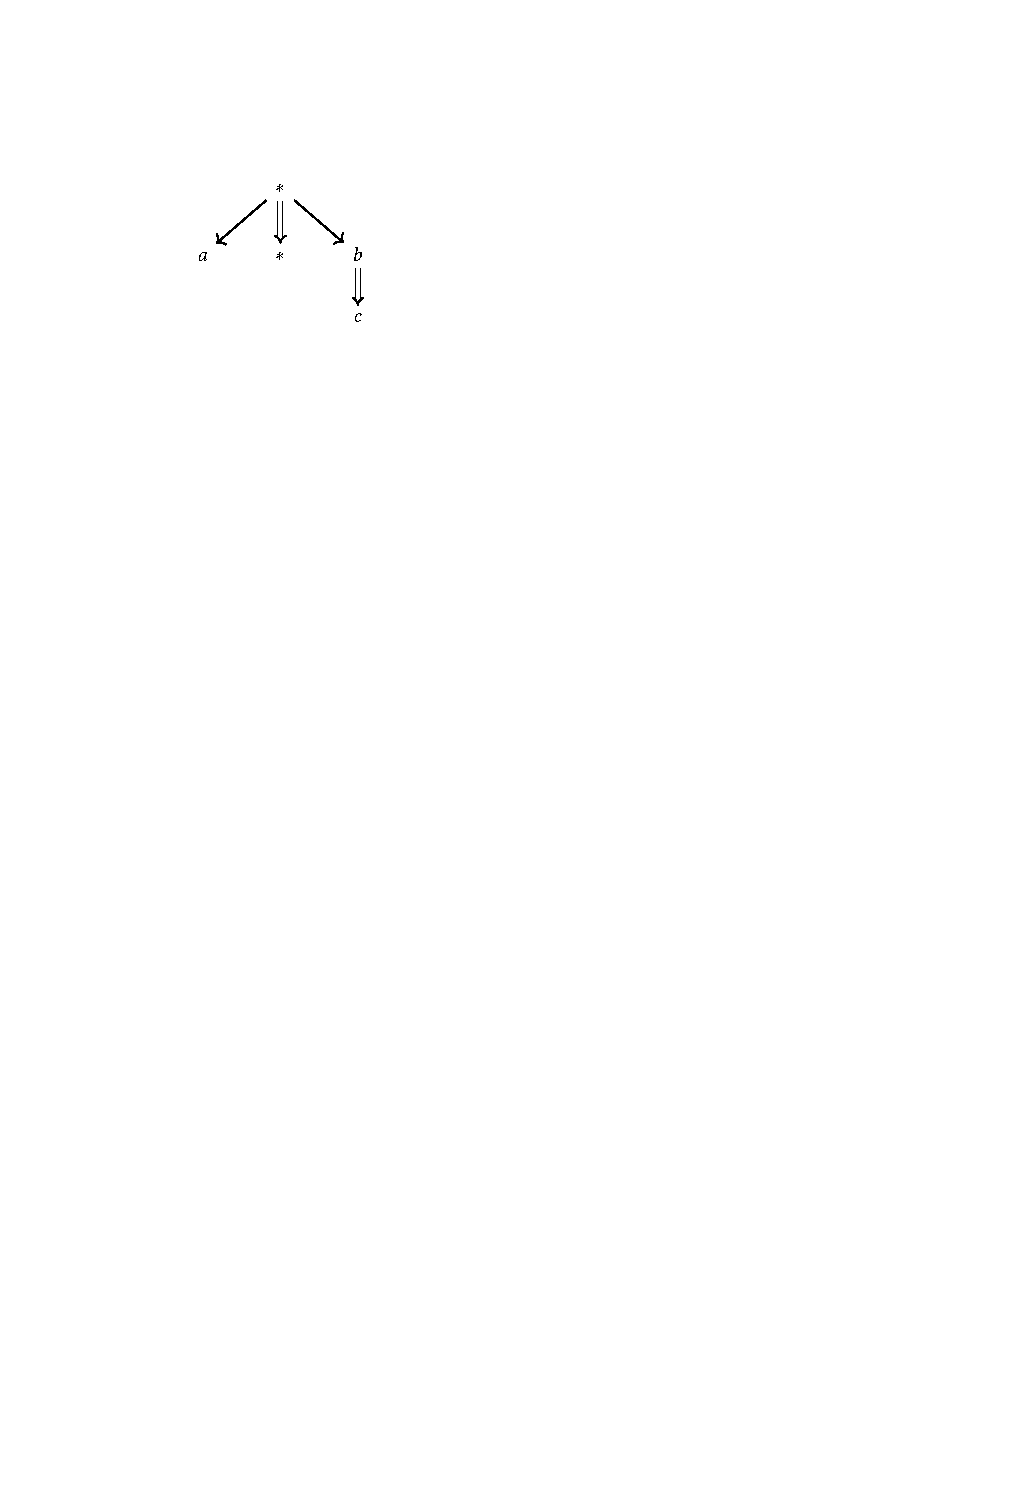
\includegraphics{fig/minimization-crpq/tree-pattern-example.pdf}
	}
	\hfil
	\subfloat[Its "encoding" $\Encoding(\tau)$ as a "CRPQ".]{
		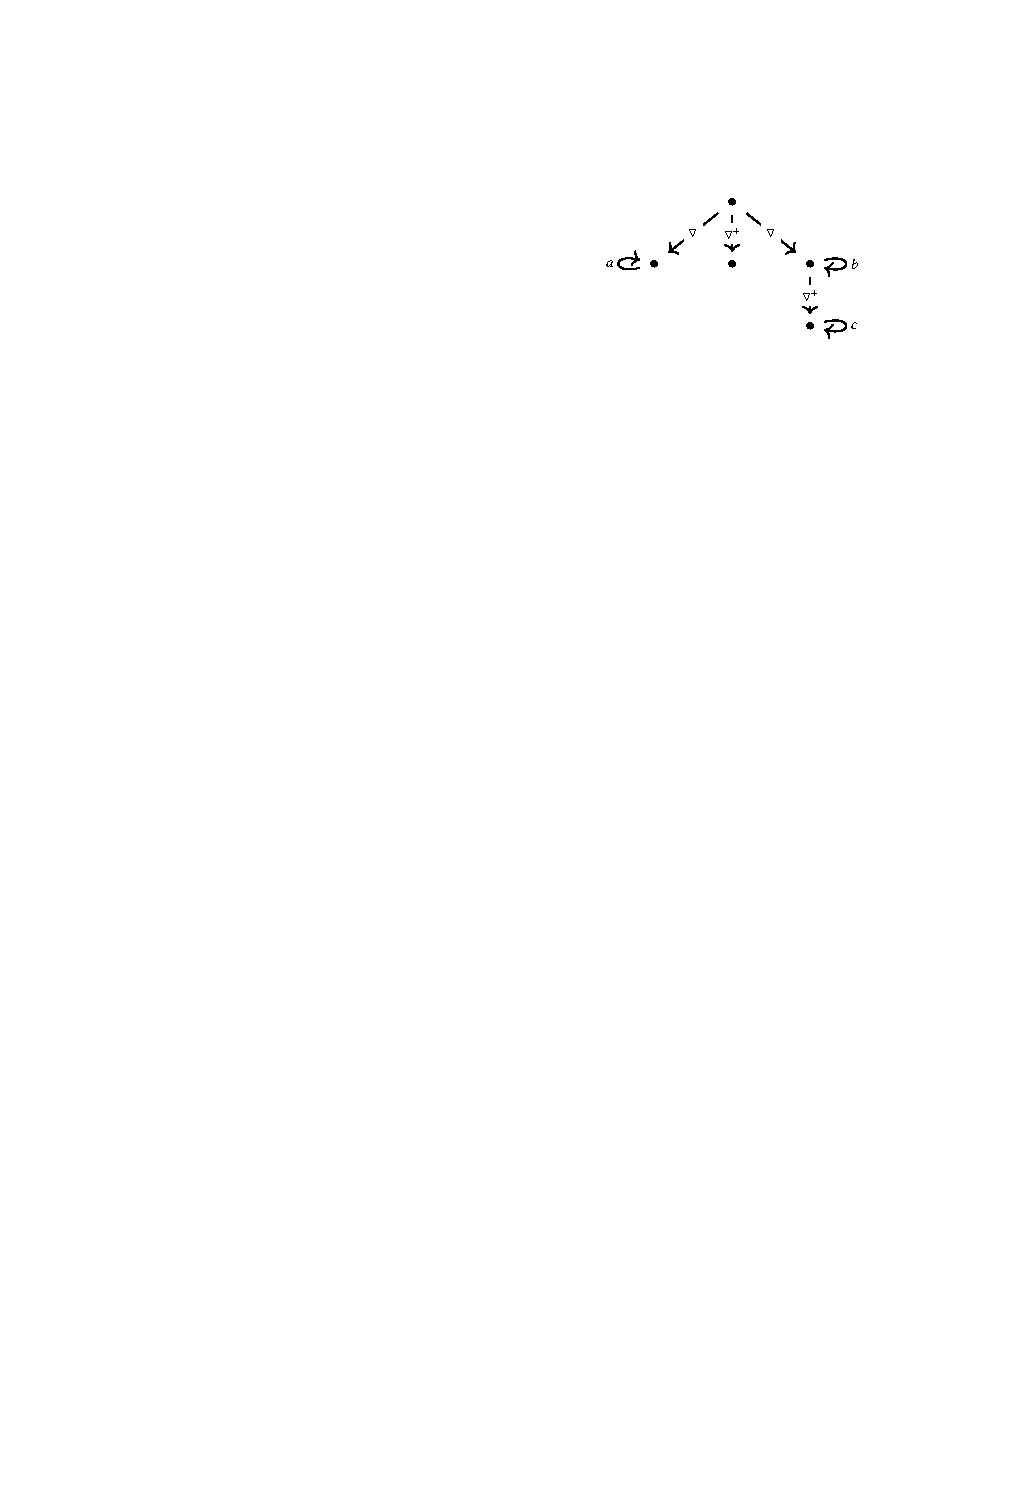
\includegraphics{fig/minimization-crpq/tree-pattern-example-enc.pdf}
	}
	\caption{
		\AP\label{fig:encoding-tree-pattern}
		"Encoding" a "tree pattern" into a "CRPQ".
	}
\end{figure}

We \AP""encode"" a "tree pattern" $\tau$ into a "CRPQ" over $\A\sqcup\{\marking\}$, denoted
by \AP$\intro*\Encoding(\tau)$, obtained as follows:
\begin{itemize}
	\item we start from the underlying tree of the "tree pattern",
		and replace simple edges by an "atom" $\qvar \atom{\marking} \qvar$,
		and transitive edges by an "atom" $\qvar \atom{\marking^+} \qvar$;
	\item for any node $x$ with a node label $a \in \A$, we add an "atom" $x \atom{a} x$;
	\item for any node with a wildcard label $*$, we do not add any "atom".
\end{itemize}
See \Cref{fig:encoding-tree-pattern} for an example. Note that this "encoding" is injective.

\begin{proposition}
	Given two "tree patterns" $\tau_1$, $\tau_2$ over $\A$, the following are equivalent:
	\begin{itemize}
		\item $\tau_1 \contained \tau_2$ as "tree patterns"---in the sense of
			\cite[Definition 2.2]{CzerwinskiMartensNiewerthParys2018Minimization}, and
		\item $\Encoding(\tau_1) \contained \Encoding(\tau_2)$ as "CRPQs".
	\end{itemize}
\end{proposition}

\begin{proof}[Proof sketch]
	This follows from the characterization of containment for "tree patterns"
	using ``canonical tree models''---see \cite[\S4.2]{CzerwinskiMartensNiewerthParys2018Minimization}\footnote{Note
	however that the authors assume the set of labels to be infinite, and label `$*$'-nodes
	by $z$-nodes where $z$ is a new label: this assumption can be removed by
	allowed unlabelled nodes in the model.}---and the characterization of "containment" for "CRPQs"
	via "canonical databases" ("aka" "expansions")---see \Cref{prop:cont-char-exp-st}.
\end{proof}

We do not fully understand the relation between tree pattern minimization and "CRPQ minimization", 
and conjecture that this encoding actually preserves minimality, but we have failed so far to prove this. 

\begin{restatable}{conjecture}{conjTreePatternsAsCRPQs}
	If a "tree pattern" is minimal among "tree patterns", 
	then its "encoding" as a "CRPQ" should also be minimal among "CRPQs", up to "contracting internal variables".
\end{restatable}

\clearpage
\begin{subappendices}
	\section{Lower Bounds for Variable Minimization}
\label{apdx-sec:lowerbound-variables}

\subsection{Equivalence with a Single Variable}

\begin{theorem}
	\AP\label{thm:variable-minimization-lowerbound}
	There is a fixed alphabet "st" the problem of, given a "Boolean CRPQ"
	on this alphabet with only five variables is "equivalent"
	to a "Boolean CRPQ" with a single variable is "ExpSpace"-hard.
\end{theorem}

\begin{proof}
	We use same idea as in \Cref{thm:minimization-lowerbound}.
	We reduce the problem of \Cref{prop:variation-figueira} to the instance $\delta$, where
	\begin{center}
        \begin{tikzcd}[column sep=scriptsize]
			&
			&
			&
			x
				\ar[dll, "\triangleright", bend right=20]
				\ar["\marking", loop above, out=120, in=60, distance=1.8em]
			&
			&
			\\[-.5em]
			\delta() = &[-2.1em]
            \qvar \ar[dr, "\A^*" swap, bend right=20] \ar[rrrr, "K"] &
			&
			&
			&
			\qvar,
				\ar[ull, "\triangleleft", bend right=20]\\[-.5em]
			&
			&
			\qvar \ar[rr, "L_1", bend left=20]
				\ar[rr, "\raisebox{6pt}{\small\vdots}", phantom]
				\ar[rr, "L_p" below, bend right=20] &
			&
			\qvar \ar[ur, "\A^*" swap, bend right=20]
        \end{tikzcd}
    \end{center}
	where $\triangleright$, $\marking$ and $\triangleleft$ are new symbols.
	Note that despite being named, variable $x$ is also existentially quantified.
	
	\begin{claim}
		\AP\label{claim:variable-minimization-lowerbound-1}
		If $\gamma_1 \contained \gamma_2$ then $\delta \semequiv \gamma'_1$
		where $\gamma'_1() \defeq x \atom{\triangleright K \triangleleft} x
		\land x \atom{\marking} x$.
	\end{claim}
	
	If $\gamma_1 \contained \gamma_2$ then any word of $K$ contains a
	factor which belongs to $\bigcap_j L_j$ and so $\gamma'_1 \contained \delta$.
	The converse $\delta \contained \gamma'_1$ always holds.

	\begin{claim}
		\AP\label{claim:variable-minimization-lowerbound-2}
		Conversely, if $\delta$ is "equivalent" to a "Boolean CRPQ" with
		a single variable, then $\gamma_1 \contained \gamma_2$.
	\end{claim}

	Let $\zeta() = \bigwedge_{i=0}^n x \atom{M_i} x$ be a single-variable "Boolean CRPQ"
	that is "equivalent" to $\delta$.

	We first claim that there is some $i \in \lBrack 0,n\rBrack$
	"st" $M_i = \{\marking\}$. Every "canonical database" of $\delta$ contains a $\marking$-self loop
	and so from $\zeta \contained \delta$ it follows that any
	"canonical database" of $\zeta$ contains a $\marking$-self loop, which in turns implies
	that $M_i = \{\marking\}$ for some $i$. "Wlog", assume that $M_0 = \{\marking\}$.
	
	Observe that any "evaluation map" from $\zeta$ to a "canonical database"
	of $\delta$ must send $x \in \zeta$ to $x \in \delta$ because of the $\marking$-self loop,
	and conversely, any "evaluation map" from $\delta$ to a "canonical database"
	of $\zeta$ must send $x \in \delta$ to $x \in \zeta$.

	We remove from $\zeta$ all atoms $x \atom{M_i} x$ "st" $i \neq 0$
	and $M_i \cap {\marking^*} \neq\emptyset$. Thanks to the
	$\marking$-self loop, this transformation preserve the semantics of $\zeta$.
	More generally, if $M_i$ contains a word in which the letter `$\marking$' occurs, we get remove 
	the atom associated to $M_i$ altogether. The query obtained $\zeta'$ is clearly
	"st" $\zeta \contained \zeta'$, but dually for any "canonical database" $G_{\zeta'}$ of
	$\zeta'$, extend it to a "canonical database" $G_{\zeta}$ of $\zeta$ by picking, for any
	atom that was removed, any word containing the letter `$\marking$'.
	Since $\zeta \contained \delta$, there is an "evaluation map" from $\delta$
	to $G_{\zeta}$. Now the atoms of $\delta$ except the $\marking$-self loop
	do not use the letter $\marking$, and so it follows that the
	"evaluation map" from $\delta$ to $G_{\zeta}$ actually yields
	an "evaluation map" from $\delta$ to $G_{\zeta'}$.
	\todo{add figure}
	Hence, $\zeta' \contained \delta$ and thus $\zeta' \semequiv \delta$.

	The same argument works for "atoms" containing a word that does not
	start with $\triangleleft$, or that does not end $\triangleright$,
	or that contain strictly more than one occurrence of these symbols.
	Overall, it implies that "wlog" $\zeta$ is "equivalent" to
	\[
		x \atom{\marking} x \land \bigwedge_{j=1}^{m} x \atom{\triangleright N_j \triangleleft} x
	\]
	where $m \geq 0$ and the $N_j$'s are languages over $\A$.

	Assume now, by contradiction, that for all $j \in \lBrack 1,m \rBrack$
	"st" $N_j \not\subseteq K \cap \A^* \big(\bigwedge_i L_i\big) \A^*$. Pick for each $j$ a word $u_j$ witnessing this. 
	The canonical database of $\zeta$ induced by these
	words $\langle n_1, \hdots, n_m \rangle$, namely
	\[x \atom{\marking} x \land \bigwedge_{j=1}^m x \atom{\triangleright n_j \triangleleft}\]
	must satisfy $\delta$. But this implies that at least one $n_j$ must belong to
	$K \cap \A^* \big(\bigcap_i L_i\big) \A^*$.
	Contradiction.
	
	In fact, a argument similar to what we claimed before shows that
	we can remove all "atoms" "st" $N_j \not\subseteq K \cap \A^* \big(\bigcap_i L_i\big) \A^*$ without changing the semantics.
	Hence, "wlog", for each $j$, we have $N_j \subseteq K \cap \A^* \big(\bigcap_i L_i\big) \A^*$.

	We then claim that each word of $K$ must belong to all $N_j$.
	Indeed, let $u$ be a word of $K$. Let $v_i$ be a word in
	$L_i \smallsetminus \A^* \big(\bigcap_k L_k\big) \A^*$---recall
	that such words exist by an assumption of \Cref{prop:variation-figueira}---and
	consider the "canonical database" of $\delta$ obtained by "expanding"
	$K$ into $u$ and $L_i$ into $v_i$.
	Now $\delta \contained \zeta$ so this database must satisfy $\zeta$.
	Hence, for each $j$, $N_j$ must contain one word among $u$, $v_1, \hdots,v_m$.
	It cannot be any $v_i$ since otherwise we would have $v_i \in N_j \subseteq
	K \cap \A^* \big(\bigcap_k L_k\big) \A^* \subseteq \A^* \big(\bigcap_k L_k\big) \A^*$, which is a contradiction. And so $u \in N_j$.
	Therefore, we have
	\[
		K \subseteq \bigcap_j N_j \subseteq K \cap \A^* \big(\bigcap_i L_i\big) \A^*
	\]
	from which it follows that $K \subseteq \big(\bigcap_k L_k\big)$ and hence
	$\gamma_1 \contained \gamma_2$.
	
	Overall,
	\Cref{claim:variable-minimization-lowerbound-1,claim:variable-minimization-lowerbound-2}
	imply that $\gamma_1 \contained \gamma_2$ "iff" it is equivalent
	to a "CRPQ" with a single variable, in which case it is actually equivalent to
	\[\gamma'_1() \defeq x \atom{\triangleright K \triangleleft} x
		\land x \atom{\marking} x,\]
	which concludes the correctness of the reduction.
\end{proof}

\subsection{Variable Minimization is Harder than Containment}

We say that the "class@@CRPQ" is \AP""closed under disjoint conjunction""
if $\gamma \in \classCRPQ_\A$ and $\delta \in \classCRPQ_\B$
imply $\gamma \disconj \delta \in \classCRPQ_{\A \cup \B}$.

Lastly, we say that the class is \AP""closed under variable marking""
if \emph{one of} the three following properties holds: 
\begin{description}
	\itemAP[\intro*\axiomVarMarkingLoop] for any $\gamma \in \classCRPQ_{\A}$, if $y$ is a variable of $\gamma$,
		if $a\not\in\A$, then $\gamma' \defeq \gamma \land y \atom{a} y$
		is in $\classCRPQ_{\A\sqcup\{a\}}$, or
	\itemAP[\intro*\axiomVarMarkingOut] for any $\gamma \in \classCRPQ_{\A}$, if $y$ is a variable of $\gamma$,	
		if $a\not\in\A$, then $\gamma' \defeq \gamma \land y \atom{a} y'$
		is in $\classCRPQ_{\A\sqcup\{a\}}$,
		where $y'$ is a new variable not occurring in $\gamma$, or
	\itemAP[\intro*\axiomVarMarkingIn] for any $\gamma \in \classCRPQ_{\A}$, if $y$ is a variable of $\gamma$,	
		if $a\not\in\A$, then $\gamma' \defeq \gamma \land y' \atom{a} y$
		is in $\classCRPQ_{\A\sqcup\{a\}}$,
		where $y'$ is a new variable not occurring in $\gamma$.
\end{description}

We will sometimes write $\gamma \in \classCRPQ$ to mean that $\gamma\in\classCRPQ_{\A}$
for some alphabet $\A$.

\begin{fact}
	Any "class@@CRPQ" defined by restricting the class of languages allowed to
	label the "atoms" is both "closed under disjoint conjunction" and "closed under variable marking", assuming that languages of
	the form $\{a\}$ are allowed, where $a$ is a single letter.
\end{fact}

\begin{theorem}
	\AP\label{thm:reduction-containment-to-variable-minimization}
	For any "class of CRPQs closed under disjoint conjunction" and
	"closed under variable marking"
	$\classCRPQ$, there is a polynomial-time reduction
	from the "containment problem" for "Boolean" queries of $\classCRPQ$ to the "CRPQ" 
	"minimization problem" restricted to queries of $\classCRPQ$. 
	The same bound applies if we add the constraint that the target "CRPQ" must also belong to $\classCRPQ$.
\end{theorem}

Say that a "CRPQ" is \AP""degenerate@@CRPQ"" if it contains an atom labelled the language $\{\varepsilon\}$.
Equivalently, it is "non-degenerate@@CRPQ" if it has at least one "canonical database"
which is "non-degenerate@@db".

\begin{fact}
	\AP\label{fact:produce-non-degenerate}
	One can turn a "degenerate CRPQ" into a "non-degenerate@@CRPQ" one by
	iteratively identifying variables adjacent to an atom $\atom{\{\varepsilon\}}$.
	This can be implemented in polynomial time.
\end{fact}

\begin{proof}[Proof of \Cref{thm:reduction-containment-to-variable-minimization}]
	We assume for now that $\classCRPQ$ satisfies
	the axiom $\axiomVarMarkingLoop$.
	Given an instance $\gamma_1() \contained^{?} \gamma_2()$ of the "containment problem" for "Boolean" queries of $\classCRPQ$,
	we assume "wlog" that $\gamma_1$ is "non-degenerate@@CRPQ" using \Cref{fact:produce-non-degenerate},
	and we reduce it to the instance $\langle \delta_1 \disconj \gamma_2, \nbvar{\delta_1} \rangle$,
	where $\delta_1$ is defined as:
	\[
		\delta_1() \defeq \gamma_1 \land \bigwedge_{x \in \vertex{\gamma_1}} x \atom{\marking_x} x
	\]
	where $\marking_x$ is a fresh letter for each $x \in \vertex{\gamma_1}$.
	The reduction works clearly in logarithmic-space,
	and clearly $\delta_1 \disconj \gamma_2 \in \classCRPQ$ since
	$\classCRPQ$ is "closed under disjoint conjunction" and $\axiomVarMarkingLoop$.
	Moreover, for it to be correct
	we need to show that $\gamma_1 \contained \gamma_2$ "iff" $\delta_1 \disconj \gamma_2$
	is "equivalent" to a "CRPQ" with at most $\nbvar{\delta_1}$ variables.

	\begin{claim}
		\AP\label{claim:reduction-containment-to-variable-minimization-1}
		If $\gamma_1 \contained \gamma_2$ then $\delta_1 \disconj \gamma_2 \semequiv \delta_1$.
	\end{claim}

	Indeed, $\gamma_1 \contained \gamma_2$ implies $\delta_1 \contained \gamma_1 \contained \gamma_2$ and so $\delta_1 \disconj \gamma_2 \semequiv \delta_1$.

	Actually this property is an ``if and only if''. For the converse, we will prove a stronger statement.

	\begin{claim}
		\AP\label{claim:reduction-containment-to-variable-minimization-2}
		If $\delta_1 \disconj \gamma_2$ is "equivalent" to a "CRPQ"
		with at most $\nbvar{\delta_1}$ variables, then $\gamma_1 \contained \gamma_2$.
	\end{claim}

	Let $\zeta$ be a "CRPQ" with at most $\nbvar{\delta_1}$ variables
	that is equivalent to $\delta_1 \disconj \gamma_2$.
	
	We claim first that for each $x \in \vertex{\zeta}$ there is a
	unique variable in $\zeta$ with a $\marking_x$-self-loop.
	Indeed, consider any "canonical database" $Z$ of $\zeta$:
	since $\zeta \contained \delta_1 \disconj \gamma_2$, there exists
	a "canonical database" $D_1$ of $\delta_1$ and $G_2$ of $\gamma_2$ "st"
	$D_1 \oplus G_2 \homto Z$ where $\oplus$ denotes the disjoint union.
	Since $D_1$ contains a $\marking_x$-self loop for each $x\in \vertex{\gamma_1}$,
	so does $Z$. Since this property holds for every $Z$, it follows that
	$\zeta$ must have a self-loop atom labelled by the singleton language $\{\marking_x\}$
	for each $x\in \vertex{\gamma_1}$.

	Now observe that no variable of $\zeta$ can be labelled by two $\marking_x$-self-loops
	with $x\in\vertex{\gamma_1}$. Indeed, $\gamma_1$ is "non-degenerate@@CRPQ", and so $\delta_1$
	is also "non-degenerate@@CRPQ", and so there
	exists a "canonical database" $D_1$ of $\delta_1$ which is "non-degenerate@@db".
	Then, pick any canonical database $G_2$ of $\gamma_2$.
	$D_1 \oplus G_2$ is a "canonical database" of $\delta_1 \disconj \gamma_2$, which is 
	equivalent to $\zeta$, so there is an "evaluation map"
	from $\zeta$ to $D_1 \oplus G_2$. If a variable of $\zeta$ had both a
	$\marking_x$- and a $\marking_y$-self-loop for $x \neq y \in \vertex{\gamma_1}$,
	then so would either $D_1$ or $G_2$. $G_2$ contains no such letters, and so it would have
	to be $D_1$. This contradicts the definition of $D_1$.
	Hence, no variable of $\zeta$ can be labelled by two $\marking_x$-self-loops.
	Together with the previous paragraph and the fact that 
	$\zeta$ has at most $\nbvar{\delta_1} = \nbvar{\gamma_1}$ variables, it follows that
	we can assume "wlog"---up to renaming the variables of $\zeta$---that
	$\vertex{\zeta} = \vertex{\gamma_1}$ and for each $x \in \vertex{\gamma_1}$,
	$x \atom{\marking_x} x$ is an "atom" of $\zeta$. Moreover, this is the only self-loop in
	$\zeta$ labelled by $\{\marking_x\}$, and for any self-loop atom $x \atom{L} x$
	we cannot have $\marking_y \in L$ for any $y \neq x \in \vertex{\gamma_1}$. 
	
	We are now ready to prove that $\gamma_1 \contained \gamma_2$.
	Let $G_1$ be a "canonical database" of $\gamma_1$, and let $D_1$ be the associated
	"canonical database" of $\delta_1$---it is obtained by adding an $\marking_x$-self-loop
	on every $x \in \vertex{\gamma_1}$.
	Pick any canonical database $G_2$ of $\gamma_2$. Since $\delta_1 \disconj \gamma_2 \contained \zeta$, there exists a "canonical database" $Z$ of $\zeta$
	"st" $Z \homto D_1 \oplus G_2$.
	But then, since $\zeta \contained \delta_1 \disconj \gamma_2$, there exists
	$D'_1$ and $G'_2$, which are "canonical databases" of $\delta_1$ and $\gamma_2$,
	respectively, "st"
	\[
		D'_1 \oplus G'_2 \homto
		Z \homto
		D_1 \oplus G_2.
	\]
	Restrict this homomorphism to $G'_2$: we obtain 
	\[
		G'_2 \homto
		Z \homto
		D_1 \oplus G_2.
	\]
	Now note that, because of the previous paragraph,
	the "homomorphism" $Z \homto D_1 \oplus G_2$ must map $x \in \vertex{Z}$  
	to $x \in \vertex{D_1}$---because of the $\marking_x$-self-loop.
	Since $D_1 \oplus G_2$ is a disjoint union, it follows that image of this
	"homomorphism" is actually included in $D_1$, and so obtain a "homomorphism"
	\[
		G'_2 \homto Z \homto D_1.
	\]
	Now of course $\marking_x$-self-loop will occur in the image of any "homomorphism"
	$Z \homto D_1$. However, in the composition $G'_2 \homto Z \homto D_1$,
	since $G'_2$ does not use any letter of the form $\marking_x$, $x\in \vertex{\gamma_1}$,
	we conclude we actually get a "homomorphism"
	\[
		G'_2 \homto G_1,
	\]
	which concludes the proof that $\gamma_1 \contained \gamma_2$
	and hence of \Cref{claim:reduction-containment-to-variable-minimization-2}.
	
	Now \Cref{claim:reduction-containment-to-variable-minimization-1,claim:reduction-containment-to-variable-minimization-2} imply that
	$\gamma_1 \contained \gamma_2$ "iff" $\delta_1 \disconj \gamma_2$ is "equivalent" to a "CRPQ"
	with at most $\nbvar{\delta_1}$ variables, which concludes the reduction under the assumption
	that $\classCRPQ$ satisfies $\axiomVarMarkingLoop$.

	To conclude, note that
	if $\classCRPQ$ satisfies either $\axiomVarMarkingOut$ or $\axiomVarMarkingIn$ then exactly the same proof works, except that the definition of $\delta_1$
	should be changed: variables will be marked using outgoing and incoming edges, respectively.
	Lastly, since $\delta_1 \in \classCRPQ$, then we have as a by-product of our proof
	that $\delta_1 \disconj \gamma_2$ is equivalent to a "CRPQ" with at most $k$ atoms
	"iff" it is equivalent to a "CRPQ" of $\classCRPQ$ with at most $k$ atoms.
	It follows that this reduction also works it we add the constraint that
	$\delta$ must be in $\classCRPQ$.
\end{proof}
\end{subappendices}
\chapter[{Semantic Tree-Width and Path-Width of Conjunctive Regular Path Queries}]{Semantic Tree-Width and Path-Width\\of Conjunctive Regular Path Queries}
\label{ch:semantic-tree-width-CRPQ}
\renewcommand\thefigure{\thechapter.\arabic{figure}}

\begin{chapterpresentation}
	\begin{abstract}
		We show that the problem of whether a query is equivalent to a query of tree-width $k$ is decidable, for the class of Unions of Conjunctive Regular Path Queries with two-way navigation (UC2RPQs). 
		A previous result by Barceló, Romero, and Vardi \cite{BarceloRomeroVardi2016SemanticAcyclicity} has shown decidability for the case $k=1$, and here we extend this result showing that decidability in fact holds for any arbitrary $k\geq 1$. 
		The algorithm is in "2ExpSpace", but for the restricted but practically relevant case where all regular expressions of the query are of the form $a^*$ or $(a_1 + \dotsb + a_n)$ we show that the complexity of the problem drops to "PiP2".
		
		We also investigate the related problem of approximating a UC2RPQ by queries of small tree-width. We exhibit an algorithm which, for any fixed number $k$, builds the maximal under-approximation of tree-width $k$ of a UC2RPQ.
		The maximal under-approximation of tree-width $k$ of a query $\gamma$ is a query $\gamma'$ of tree-width $k$ which is contained in $\gamma$ in a maximal and unique way, that is, such that for every query $\gamma''$ of tree-width $k$, if $\gamma''$ is contained in $\gamma$ then $\gamma''$ is also contained in $\gamma'$.
		
		Our approach is shown to be robust, in the sense that it allows also to test equivalence with queries of a given path-width, it also covers the previously known result for $k=1$, and it allows testing whether a (one-way) UCRPQ is equivalent to a UCRPQ of a given tree-width (or path-width).
	\end{abstract}
	\par\bigskip\bigskip
	\begin{acknowledgements}
		This chapter is mostly a reproduction of the eponymous paper that was published in LMCS
		\cite{FigueiraMorvan2025SemanticTreeWidthLMCS}, as a selected paper from ICDT '23
		\cite{FigueiraMorvan2023SemanticTreeWidthICDT}.
		Part of the preliminaries and of the introductions have been moved to \Cref{ch:prelim-graph-databases}.
		It is a joint work with Diego Figueira.
	\end{acknowledgements}
	\clearpagepresentation
	\chaptertocstandalone
\end{chapterpresentation}

{
	\graphicspath{{./fig/semantic-tw}}
	\renewcommand\thefigure{\thechapter.\arabic{figure}}
	\section{\AP{}Introduction}
\label{sec:intro}

\subsection{\AP{}Graph Databases}

"Graph databases" have gained significant attention due to their ability to efficiently model and manage complex, interconnected data. Unlike traditional relational databases, they model data as entities connected by edges that represent relationships. This structure facilitates the analysis of highly interconnected data, where the topology of the connections is as crucial as the data itself, making them particularly well-suited for use cases like biology, social networks, banking, recommendation systems, and fraud detection. We refer the reader to \cite{Barcelo2013Querying,Wood2012Query,AnglesEtal2017Foundations} for surveys on the foundations and applications of graph databases.


% \footnote{This paragraph was partially written with the help of ChatGPT.}
% The growing need to handle large-scale,
% dynamic datasets with intricate relationships motivates further exploration of this model,
% as it provides both scalability and performance benefits in contexts where relationships between data points are central.

\AP ""Graph databases"" are abstracted as edge-labelled directed graphs
$G = \langle \vertex{G}, \edges{G} \rangle$, 
where nodes of $\intro*\vertex{G}$ represent entities and labelled edges $\intro*\edges{G} \subseteq \vertex G \times \A \times \vertex G$
represent relations between these entities, with $\A$ being a fixed finite alphabet.
For instance, \Cref{fig:example-graph-database} depicts a "graph database",
whose nodes are authors and papers, on the alphabet
$\A = \{\text{\color{wrote}wrote},\,\text{\color{advised}advised}\}$.
Edges $x \atom{\wrote} y$ indicate that the person $x$ wrote the paper $y$,
while edges $x \atom{\advised} y$ indicate that person $x$ was
the Ph.D. advisor of person $y$.

\begin{figure}[ht]
    \centering
    \begin{tikzpicture}
        \node (a1) {author$_1$};
        \node (a2) [right = of a1] {author$_2$};
        \node (a3) [right = of a2] {author$_3$};
        \node (a4) [right = of a3] {author$_4$};
        \node (a5) [right = of a4] {author$_5$};
        \node (p1) [below = 2.5em of a2] {paper$_1$};
        \node (p2) [below = 2.5em of a3] {paper$_2$};
        \node (p3) [below = 2.5em of a4] {paper$_3$};

        \draw[wrote] (a1) to[edge, ->] node[fill=white] {\footnotesize wrote} (p1)
            (a2) to[edge, ->] node[fill=white] {\footnotesize wrote} (p1)
            (a2) to[edge, ->] node[fill=white] {\footnotesize wrote} (p2)
            (a3) to[edge, ->] node[fill=white] {\footnotesize wrote} (p2)
            (a4) to[edge, ->] node[fill=white] {\footnotesize wrote} (p3)
            (a5) to[edge, ->] node[fill=white] {\footnotesize wrote} (p3);
        \draw[advised] (a4) to[edge, ->, bend right=60] node[fill=white] {\footnotesize advised} (a3)
            (a5) to[edge, ->, bend right=60] node[fill=white] {\footnotesize advised} (a4);
    \end{tikzpicture}
    \caption{%
        \AP\label{fig:example-graph-database}%
        A "graph database" with eight nodes and eight edges on a two-letter alphabet.
    }
\end{figure}

\AP Being a subclass of relational databases, "graph databases" can be queried by the
predominant query language of ""conjunctive queries"", "aka" "CQs", 
which consists of the closure under projection---"aka" existential quantification---of conjunctions of atoms of the form $x \atom{a} y$
for some letter $a \in \A$. For instance, the "conjunctive query"
\[
    \gamma_1(x, y) = x \atom{\wrote} z
        \land y \atom{\wrote} z    
\]
returns, when "evaluated" on the "graph database" $G$
defined in \Cref{fig:example-graph-database}, all pairs of nodes $(u, v)$ such that $u$ is a co-author
of $v$. Each variable not appearing in the left-hand side of 
the definition of a "conjunctive query" (in this example, $z$) is implicitly 
existentially quantified. 
Note that, to the cost of losing the information of which variable is existentially quantified, every "CQ"
can be seen as a "graph database", where each variable is a node, and each atom is an edge; 
hence, we sometimes use "graph database" terminology for "CQs".

The expressive power of "CQs" is somewhat limited, since
"CQs" cannot express, for example, transitive closure.
Since the ability to navigate paths is of importance in many "graph database" 
scenarios, most modern graph query languages support, as a central querying mechanism,
"conjunctive regular path queries", or "CRPQs" for short. 
In particular, "CRPQs" form the core navigational mechanism of the new ISO standard Graph Query Language (GQL) \cite{ISO2024GQL} and the SQL extension for querying graph-structured data SQL/PGQ \cite{ISO2023PGQ} (see also \cite{FrancisEtal2023GPCIcdt,FrancisEtal2023GPC}).

"CRPQs" are 
defined analogously to "conjunctive queries", except that their atoms are now of the form 
$x \atom{L} y$ where $L$ is an arbitrary regular language over the alphabet $\A$. For 
instance the "evaluation" of the "CRPQ"
\[
    \gamma_2(x, y) = x \atom{\wrote} z
        \land z' \atom{\wrote} z 
        \land y \atom{({\advised})^*} z'
\]
on $G$ yields every pair of persons $(u,v)$ such that $u$ is a co-author of a
``scientific descendant'' of $v$. 

\AP Formally, a ""CRPQ"" $\gamma$ is defined as a tuple $\bar z = (z_1,\hdots,z_n)$
of ""output variables"", "aka" \reintro{free variables},\footnote{For technical reasons (see the definition of "equality atoms") we allow for a variable to appear multiple times.}
together with a conjunction of ""atoms"" of the form
$\bigwedge_{j=1}^m x_j \atom{L_j} y_j$, where each $L_j$ is a regular language and where $m \geq 0$.
The set of all variables occurring in $\gamma$, namely\footnote{We neither assume 
disjointness nor inclusion between $\{z_1,\hdots,z_n\}$ and $\{x_1,y_1,\hdots,x_m,y_m\}$}
$\{z_1,\hdots,z_n\}\cup\{x_1,y_1,\hdots,x_m,y_m\}$, is denoted by
$\intro*\vars(\gamma)$.
Given a "database@@graph" $G$, we say that a tuple of nodes $\bar u = (u_1,\hdots,u_n)$
\AP""satisfies@@db"" $\gamma$ 
on $G$ if there is a mapping
$\fun\colon \vars(\gamma) \to \vertex{G}$ such that $u_i = \fun(z_i)$ for all
$1 \leq i \leq n$, and for each $1 \leq j \leq m$,
there exists a path from $\fun(x_i)$ to $\fun(y_i)$ in $G$, labelled by
a word from $L_i$ (if the path is empty, the label is $\epsilon$). The \AP""evaluation"" of $\gamma$ on $G$ is then the set of all tuples that "satisfy@@db" $\gamma$.
%
For example, $(\text{author}_2, \text{author}_5)$ "satisfies@@db" $\gamma_2$ 
on the "graph database" $G$ of \Cref{fig:example-graph-database} via
the function that maps $x$ to $\text{author}_2$, $y$ to $\text{author}_5$,
$z$ to $\text{paper}_2$, and $z'$ to $\text{author}_3$.

\AP
The language of "CRPQ" can be extended to navigate edges in both directions. 
\knowledgenewrobustcmd{\Gpm}{\cmdkl{G^\pm}}
Consider the expanded database $\intro*\Gpm$ obtained from $G$ by 
% keeping the same vertices, copying the edges of $G$, and 
adding, for every edge $x \atom{a} y$ in $G$, an extra edge $y \atom{a^-} x$.
We obtain a graph database on the alphabet $\intro*\Aext = \A \cup \A^-$ where
$\A^- = \set{a^- \mid a \in \A}$. We then define the syntax of
a \AP""CRPQ with two-way navigation"", or \reintro{C2RPQ}, as a "CRPQ" on the alphabet $\Aext$.
Its \reintro{evaluation} is defined as the "evaluation" of the "CRPQ" on $\Gpm$.
For instance, the "evaluation" of the "C2RPQ"
\[
    \gamma_3(x, y) = x \atom{({\wrote}\cdot{\wrote}^-)^*} y
\]
on the "graph database" of \Cref{fig:example-graph-database} returns all pairs of
individuals linked by a chain of co-authorship.
It includes $(\text{author}_1, \text{author}_3)$ or $(\text{author}_1, \text{author}_1)$
but not $(\text{author}_1, \text{author}_4)$.
%
\AP If a query has no "output variables" we call it ""Boolean"", and
its "evaluation" can either be the set $\set{()}$, in which case we say that $G$
\reintro(db){satisfies} the query, or the empty set $\set{}$. For example, $G$ "satisfies@@db" the
"Boolean CRPQ"
\[\gamma_4() = x \atom{\wrote} y\]
if, and only if, the database contains one author together with one paper they wrote.

To simplify proofs, we assume that all the regular languages are described via 
non-deterministic  finite automata (NFA) instead of regular expressions,
which does not affect any of our complexity bounds.
However, for readability all our examples will be given in terms of regular expressions.
We denote the set of "atoms" of a "C2RPQ" $\gamma$ by \AP$\intro*\atoms\gamma$, and by 
$\intro*\nbatoms{\gamma}$ we denote its number of "atoms", "ie", $|\atoms\gamma|$.
Moreover, we denote by $\intro*\size{\gamma}$ the sum of its number of "atoms" with
the sum of the size of NFAs used to describe $\gamma$.


\AP Finally, a ""union of CQs"" (\reintro{UCQs}) (resp.\ ""union of CRPQs"" (\reintro{UCRPQs}), resp.\ ""union of C2RPQs"" (\reintro{UC2RPQs}))  
is defined as a finite set of "CQs" (resp.\ "CRPQs", resp.\ "C2RPQs"), whose
tuples of "output variables" have all the same arity. 
\AP
A ""subquery"" of a "C2RPQ" $\gamma$ is any "C2RPQ" resulting from removing some "atoms" (possibly none) from $\gamma$. A \reintro{subquery} of  "UC2RPQ" is a union of "subqueries" of the "C2RPQs" therein.
The "evaluation" of a union is defined as the union of its "evaluations", for instance the following "UCQ"
\begin{align*}
    \Gamma_5 & = \gamma_{5}^1(x, y) \lor \gamma_{5}^2(x, y) \\
    & \text{ where }
    \gamma_{5}^1(x, y) = x \atom{\wrote} y %\\
    \text{ and }
    \gamma_{5}^2(x, y) = x \coatom{\advised} z \land
        z \atom{\wrote} y
\end{align*}
"evaluates" to the set of pairs $(x,y)$ such that $y$ is a paper written by either $x$
or their advisor.
We naturally extend the notations $\nbatoms{-}$ and $\size{-}$ to "unions@UC2RPQs".
\AP ""Infinitary unions"" are defined analogously, except
that we allow for potentially infinite unions. We often use a set notation to denote the union, especially for "infinitary unions".

For a more detailed introduction to "CRPQs", we refer the reader to \cite{Figueira2020Containment21Foundations}.
For a more general introduction to different query languages for "graph databases"---including "CRPQs"---see \cite{Barcelo2013Querying}, and for a more practical approach,
see \cite{AnglesEtal2017Foundations}.

\smallskip

% \paragraph*{Containement and equivalence}
\AP %It is often interesting to compare queries together. 
The ""evaluation problem"" for "UC2RPQ" is the problem of, given
a "UC2RPQ" $\Gamma$, a "graph database" $G$ and a tuple $\bar u$ of elements of $G$,
whether $\bar u$ "satisfies@@db" $\Gamma$ on $G$. 
Given two "UC2RPQ" $\Gamma$
and $\Gamma'$ whose "output variables" have the same arity,
we say that $\Gamma$ is \AP""contained"" in $\Gamma'$,
denoted by $\Gamma \intro*\contained \Gamma'$ if
for every "graph database" $G$, for every tuple $\bar u$ of $G$,
if $\bar u$ "satisfies@@db" $\Gamma$ on $G$, then so does $\Gamma'$ (we will hence reserve the symbol `$\subseteq$' for set inclusion---note in particular that inclusion (of the "UC2RPQs", seen as sets of "C2RPQs") implies "containment", but the converse does not hold). 
The \AP""containment problem"" for "UC2RPQs" is the problem of, given
two "UC2RPQs" $\Gamma$ and $\Gamma'$, to decide if $\Gamma \contained \Gamma'$.
When $\Gamma$ is "contained" in $\Gamma'$ and vice versa, we say that
$\Gamma$ and $\Gamma'$ are \AP""semantically equivalent"", denoted by
$\Gamma \intro*\semequiv \Gamma'$.  

\paragraph{Queries of small tree-width}
It is known that the "evaluation problem" for "UC2RPQ" is "NP"-complete, just as for "conjunctive queries"
\cite[Theorem 7]{ChandraMerlin1977Implementation}.
However, queries whose underlying structure looks like a tree---formally, queries of bounded 
"tree-width"---can be "evaluated" in polynomial time \cite[Theorem 3]{ChekuriRajaraman2000Containment}.\footnote{Theorem 3 talks about query "containment" of "CQs", which is in fact equivalent to the "evaluation problem" for "CQs". Moreover, the theorem deals with ``query width'', but this parameter is equivalent up to a multiplicative constant to the "tree-width" \cite[Lemma 2]{ChekuriRajaraman2000Containment} assuming that the database signature arity is fixed.} 

\AP
"Tree-width" is a measure of how much a
graph differs from a tree, introduced by Arnborg, Corneil and
Proskurowski~\cite{ArnborgCorneilProskurowski1987Complexity}.
% who noticed that many "NP"-complete problems become polynomial-time solvable on classes of graphs of bounded tree-width \cite{ArnborgCorneilProskurowski1987Complexity}.
%
For a gentle but thorough introduction to "tree-width", we refer the reader to
\cite[\S 3.6]{NesetrilPOM2012Prolegomena}. Formally, a \AP""tree decomposition"" of a multigraph $G$ is a
pair $(T, \intro*\bagmap)$ where $T$ is a tree and $\bagmap: \vertex{T} \to \pset{\vars(G)}$ is a function that associates to each node of $T$, called \AP""bag"",
a set of vertices of $G$. When $x \in \bagmap(b)$ we shall say that the "bag"
$b \in \vertex{T}$ \AP""contains@@tw"" vertex $v$. Further, it must satisfy the following three properties:
\begin{itemize}
    \item each vertex $v$ of $\gamma$ is "contained@@tw" in at least one "bag" of $T$;
    \item for each edge $u \atom{} v$ of $G$, there is at least one "bag" of $T$
        that "contains@@tw" both $u$ and $v$; and 
    \item for each vertex $v$ of $G$, the set of bags of $T$ "containing@@tw" $v$ is a 
        connected subset of $\vertex{T}$.
\end{itemize}
The \AP""width"" of $(T, \bagmap)$ is the maximum of $|\bagmap(b)|-1$ when $b$ ranges over
$\vertex{T}$.

\begin{figure}
	\centering
	\subfloat[``Full'' representation of $(T, \bagmap)$.]{%
		\AP\label{fig:ex-tree-dec-full}
		\includegraphics[scale=.5]{ex-tree-dec-full.pdf}%
	}
	\hfill
	\subfloat[``Concise'' representation of $(T, \bagmap)$]{%
		\AP\label{fig:ex-tree-dec-concise}
		\includegraphics[scale=1.1]{ex-tree-dec-concise.pdf}
	}
	\caption{
		\AP\label{fig:ex-tree-dec}
		Two different representations of the same "tree decomposition" $(T, \bagmap)$ of a 
		multigraph $G$ with six 
		vertices. The underlying tree is a path with four nodes and each "bag" contains 3 
		vertices---hence the "decomposition@tree decomposition" has "width" 2.
	}
\end{figure}
We give an example of "tree decomposition" in \Cref{fig:ex-tree-dec}:
\begin{itemize}
	\item In \Cref{fig:ex-tree-dec-full}, we give the ``full'' representation of
	the "decomposition@tree decomposition": we draw $T$, and inside each "bag" $b$ of $T$
	we represent a copy of $G$. Nodes of $G$ belonging to $b$ are highlighted, while the others are dimmed. Sometimes, we will only write the
	name of the nodes contained in the "bag", instead of drawing the graph.
	\item In \Cref{fig:ex-tree-dec-concise}, we give a ``concise'' representation:
	we draw over $G$ a coloured shape for each "bag" of $T$. This representation is ambiguous---the structure of $T$ is not made explicit---and will only be used when no ambiguity can arise.
\end{itemize}

The \AP""tree-width"" of $G$ is the minimum of the "width" of all "tree decompositions" of $G$. The \reintro{tree-width} of a "C2RPQ" is the "tree-width" of its underlying multigraph. 
We denote by $\intro*\Tw$ (resp.\ $\intro*\TwOneWay$) the set of all "C2RPQs" (resp.\ "CRPQs") of "tree-width" at most $k$. The \reintro{tree-width} of a "UC2RPQ" is simply the maximum of the "tree-width" of its "C2RPQs".
\AP
A ""path decomposition"" is a "tree decomposition" $(T,\bagmap)$ in which $T$ is a path. The \AP""path-width"" of $\gamma$ is the minimum of the "width" among all "path decompositions" of $\gamma$. The \reintro{path-width} of a "C2RPQ" and "UC2RPQ" are defined analogously. We denote by \AP$\intro*\Pw$ (resp.\ $\intro*\PwOneWay$) the set of all "C2RPQs" (resp.\ "CRPQs") of "path-width" at most $k$. The relationship between these classes is depicted in \Cref{fig:taonomy-syntactic}:
note that $\TwOneWay$ and $\PwOneWay$ are not explicitly drawn, but correspond to the
intersection of $\Tw$ (resp.\ $\Pw$) with the class of "CRPQs".

\begin{figure}
	\centering
	\scalebox{1.125}{
	\begin{tikzpicture}
		\node at (0,0) {\includegraphics[scale=.8]{taxonomy-syntactic.pdf}};
		% \draw[line width=1.5pt] (0,-4) -- (0,4);
		% \draw[line width=1.5pt] (-3,0) -- (3,0);
		% \draw[line width=.5pt] (1,-4) -- (1,4);
		% \draw[line width=.5pt] (-3,1) -- (3,1);
		% \draw[line width=.5pt] (-1,-4) -- (-1,4);
		% \draw[line width=.5pt] (-3,-1) -- (3,-1);
		\node[font=\small] at (.5,-1.5)
			{$\withkl{\kl[\Pw]}{\cmdkl{\color{cYellow}\mathcal{P\hspace{-.15em}w}_{1\!}}}$};
		\node[font=\small] at (-.5,0) 
			{$\withkl{\kl[\Pw]}{\cmdkl{\color{cYellow}\mathcal{P\hspace{-.15em}w}_{k\!}}}$};
		\node[font=\small] at (2.05,.2)
			{$\withkl{\kl[\Tw]}{\cmdkl{\color{cBlue}\mathcal{T\hspace{-.15em}w}_{1\!}}}$};
		\node[font=\small] at (1.4,1.8)
			{$\withkl{\kl[\Tw]}{\cmdkl{\color{cBlue}\mathcal{T\hspace{-.15em}w}_{k\!}}}$};
		\node[font=\tiny] at (-1.5,.5) {\kl[CRPQ]{\color{cDarkGrey}CRPQs}};
		\node[font=\tiny] at (-.5,2.4) {\kl[C2RPQ]{\color{cDarkGrey}C2RPQs}};
	\end{tikzpicture}
	}
	\caption{
		\AP\label{fig:taonomy-syntactic}
		Clickable taxonomy of syntactic classes studied in this paper.
	}
\end{figure}

Similar statements of the following proposition can be considered Folklore (see "eg" {\cite[Theorem IV.3]{RomeroBarceloVardi2017Homomorphism}}); however, our inability to find a proof for it with sharp bounds invites us to include a proof.
\begin{restatable}[Proof in \Cref{apdx-sec:prop:crpq-bound-tree-width-upper-bound}]{proposition}{crpqboundtwupperbound}
	\AP\label{prop:crpq-bound-tree-width-upper-bound}
    For each $k \geq 1$, the "evaluation problem" for "UC2RPQs" of "tree-width" at
    most $k$ can be solved in time $\+O(\size{\Gamma} \cdot |G|^{k+1} \cdot \log{|G|})$ on a Turing machine,
	or $\+O(\size{\Gamma} \cdot |G|^{k+1})$ under a RAM model, where $\Gamma$ and $G$ are the input "UC2RPQ" and "graph database", respectively.
\end{restatable}



In practice, "graph databases" tend to be huge and often changing, while queries
are in comparison very small.
This motivates the following question, given some natural $k \geq 1$: 

\begin{center}
    \AP 
    Given a "UC2RPQ" $\Gamma$, is it "equivalent" to a "UC2RPQ" $\Gamma'$ of "tree-width" at most $k$?\\
    That is, does it have ""semantic tree-width"" at most $k$?
\end{center}
This problem is called the ""semantic tree-width $k$ problem"".
Should it be decidable in a constructive way---that is, decidable, and if the answer is positive, we can compute a witnessing $\Gamma'$ from $\Gamma$---, then one could, once and for all,
compute $\Gamma'$ from $\Gamma$ and, whenever one wants to "evaluate" $\Gamma$ on a
database, "evaluate" $\Gamma'$ instead.

We will also study the restriction of these notions to one-way queries: a "UCRPQ" has \AP""one-way semantic tree-width"" at most $k$ if it is equivalent to a "UCRPQ" of "tree-width" at most $k$. The \AP""one-way semantic tree-width $k$ problem"" is the problem of, given a "UCRPQ" $\Gamma$, whether it has "one-way semantic tree-width" at most $k$.

\begin{example}
    \AP\label{ex:CRPQ-tw3-stw2}
    Consider the following "CRPQs",\footnote{In this graphical representation,
	we interpret a labelled graph as the "CRPQ" defined as
	the conjunction of the "atoms" induced by the labelled edges of the graph.
	For instance, $\gamma(\bar x)$ is a conjunction of six "atoms".}
    where $\bar x = (x_0,x_1,y,z)$:\leavevmode
    \begin{center}
        \small
        \begin{tikzcd}[column sep=small, row sep=small]
            &[-.5em] x_0 \ar[dr, "a"] \ar[rr, "c"] \ar[ddr, "a(bb)^+" swap, pos=.6, bend right] & &
            x_1 \ar[dl, "a" swap] \ar[ddl, "ab(bb)^*", pos=.7, bend left]
                &[1.5em] &[-.5em] x_0 \ar[dr, "a"] \ar[rr, "c"] \ar[ddr, "a(bb)^+" swap, pos=.6, bend right] & &
                x_1 \ar[dl, "a" swap] 
                    &[1.5em] &[-.5em] x_0 \ar[dr, "a"] \ar[rr, "c"]  & &
                    x_1 \ar[dl, "a" swap] \ar[ddl, "ab(bb)^*", pos=.6, bend left] \\
            \gamma(\bar x) \defeq & & y \ar[d, "b^+", pos=.35] & 
                & \delta(\bar x) \defeq & & y \ar[d, "b(bb)^*" pos=.35] & 
                    & \delta'(\bar x) \defeq & & y \ar[d, "(bb)^+" swap, pos=.35] & \\
            & & z & 
                & & & z & 
                    & & & z &
        \end{tikzcd}
    \end{center}
    \noindent
    The underlying graph of $\gamma(\bar x)$ being the directed 4-clique, $\gamma 
    (\bar x)$ has "tree-width" 3. We claim that $\gamma(\bar x)$ is equivalent to the "UCRPQ"
    $\delta(\bar x) \lor \delta'(\bar x)$, and hence has "one-way semantic tree-width" at most 2.

    Indeed, given a "graph database" satisfying $\gamma(\bar x)$ via some mapping $\mu$, 
    it suffices to make a case disjunction on whether the number of $b$-labelled "atoms"
    in the path from
    $\mu(y)$ to $\mu(z)$ is even or odd. In the first case, the "atom" $x_0\atom{a(bb)^+} z$ becomes
    redundant since we can deduce the existence of such a path from the conjunction
    $x \atom{a} y \atom{(bb)^+} z$, and hence the "database@@graph" "satisfies@@db" $\delta(\bar x)$ via $\mu$.
    Symmetrically, in the second case, the "atom" $x_1 \atom{b(bb)^*} z$ becomes redundant,
    and the "database@@graph" "satisfies@@db" $\delta'(\bar x)$ via $\mu$. 
    Thus, $\gamma(\bar x)$
    is "contained", and hence "equivalent" (the other "containment" being trivial), to
    the "UCRPQ" $\delta(\bar x) \lor \delta'(\bar x)$ of "tree-width" 2.
\end{example}

\subsection{\AP{}Related Work}
\label{sec:relwork}
On the class "conjunctive queries", the "semantic tree-width $k$ problem" becomes the "coNP"-complete problem of finding out whether the retraction of a query has "tree-width"
at most $k$. In fact, "CQs" enjoy the effective existence of unique minimal queries \cite[Theorem 12]{ChandraMerlin1977Implementation}, which happen to also minimize the tree-width. For "CRPQs" and "UC2RPQs", the question is far more challenging, and it has only been solved for the case $k = 1$ 
by Barceló, Romero, and Vardi \cite[Theorem 6.1]{BarceloRomeroVardi2016SemanticAcyclicity}; the case $k>1$ was left widely open
\cite[\S 7]{BarceloRomeroVardi2016SemanticAcyclicity}.

Furthermore, classes of "CQs" of bounded "semantic tree-width" precisely characterize tractable (and "FPT") "evaluation problem" \cite[Theorem~1.1]{Grohe2007ComplexityHomomorphism}.
This result is on bounded-arity schemas, which was later generalized \cite[Theorem~1]{ChenGottlobLanzingerPichler2020Semantic} for characterizing "FPT" "evaluation" on arbitrary schemas---by replacing "semantic tree-width" with semantic ``submodular width'' \cite{Marx13Tractable}.

The problem of computing "maximal under-approximations" of "CQs" of a given "tree-width" has been explored in \cite{BarceloLibkinRomero2014Efficient}.
A "maximal under-approximations" of tree-width at most $k$ of a "CQ" $\gamma$ consists of a
"CQ" $\delta_k$ of "tree-width" at most $k$, which under-approximates it,
"ie" $\delta_k$ is "contained" in $\gamma$, and which is maximal, in the sense that for every "CQ" 
$\delta'$, if $\delta'$ has "tree-width" at most $k$ and is "contained" in $\gamma$, then 
$\delta'$ is "contained" in $\delta_k$. 
"Maximal under-approximations" of a given "tree-width" for "CQs" always exist \cite{BarceloLibkinRomero2014Efficient} and thus, a "CQ" is "semantically equivalent"
to a "CQ" of "tree-width" at most $k$ if, and only if, it is equivalent to its maximal under-approximation of "tree-width" at most $k$. Our solution to decide the
"semantic tree-width $k$ problem" for "UC2RPQs" is based on this idea.

While "maximal under-approximations" always exist for "CQs", this is not the case for the dual notion of ``minimal over-approximations''. The problem of when these exist is still unknown to be decidable, aside for some the special cases of acyclic "CQs" and Boolean "CQs" over binary schemas \cite{BarceloRomeroZeume2020Approximation}.


\subsection{\AP{}Contributions}
% \remi{Please check this subsection. I had to move some paragraphs around ("closed under sublanguages") was defined after its first use.}
Here we solve both the "semantic tree-width $k$ problem" and "one-way semantic tree-width $k$ problem" for every $k$ with one unifying approach.
\begin{theorem}
    \AP\label{thm:decidability-semtw}
    For each $k \geq 1$, the "semantic tree-width $k$ problem" and the "one-way semantic tree-width $k$ problem" are decidable. Moreover, these problems are in "2ExpSpace" and are "ExpSpace"-hard.
	When $k=1$, the problems are in fact "ExpSpace"-complete.
\end{theorem}
In \Cref{sec:maximal-under-approximations} (\Cref{lem:sem-tw-in-twoexp}),
we prove the upper bound for $k\geq 2$, by relying on the so-called ``"Key Lemma"'', which is our main technical result, and is proven in \Cref{sec:treedec,sec:proof-key-lemma}.
The upper bound for the case $k=1$---which was already proven in \cite{BarceloRomeroVardi2016SemanticAcyclicity} for the (two-way) "semantic tree-width $1$ problem"---is shown in \Cref{sec:acyclic-queries} (\Cref{cor:sem-tw-1-pb-exp-c}). The lower bound is shown in \Cref{sec:lowerbound} (\Cref{lemma:lowerbound}).

The "Key Lemma" (\Cref{lemma:bound_size_refinements}) essentially states that
every "UC2RPQ" has a computable ``maximal under approximation'' by a "UC2RPQ" of "tree-width" $k$ and that this approximation is well-behaved with respect to the class of languages used to label the queries under some mild assumptions on it (being ``"closed under sublanguages"''). Let us first
explain this assumption before formalizing the statement above (stated as \Cref{cor:mua-exists-effective}).

For a class $\+L$ of languages, let $\intro*\UCtwoRPQ(\+L)$ denote the class of all "UC2RPQs" whose atoms are all labelled by languages from $\+L$.
\AP For an NFA $\+A$ and two states $q,q'$ thereof, we denote by $\intro*\subaut{\+A}{q}{q'}$ the ""sublanguage"" of $\+A$ recognized  when considering $\set{q}$ as the set of initial states and $\set{q'}$ as the set of final states.
\AP We say that $\+L$ is ""closed under sublanguages"" if
(i) it contains every language of the form $\{a\}$,
where $a \in \A$ is any (positive) letter such that either $a$ or $a^-$ occur in a word of a
language of $\+L$, and (ii) for every language $L \in \+L$ there exists an NFA $\+A_L$ accepting $L$ such that every "sublanguage" $\subaut{\+A_L}{q}{q'}$ distinct from $\emptyset$ and
$\{\varepsilon\}$ belongs to $\+L$.

To the best of our knowledge,
all classes of regular expressions that have been considered in the realm of regular path queries (see, "eg", \cite[\S1]{FigueiraEtal2020Containment}) are "closed under sublanguages". In particular, this is
the case for the class $\bigl\{ \{a_1+\hdots+a_n\} \mid a_1,\hdots,a_n
\in \A \bigr\} \cup \bigl\{ a^* \mid a \in \A \bigr\}$, which will be our focus of study in \Cref{sec:sre}. Moreover, even if some class $\+L$
is not "closed under sublanguages", such as $\{(aa)^*\}$,
then it is contained in a minimal class "closed under sublanguages"---$\{a, a(aa)^*, (aa)^*\}$ in 
this example.

We can now state the main implication of the "Key Lemma" (whose formal statement requires some extra definitions).
\begin{restatable*}[Existence of the "maximal under-approximation"]{cor}{muaexistseffective}
    \AP\label{cor:mua-exists-effective}
    % Fix $k > 1$ and a class $\+L$ of regular languages closed under "sublanguages". Then, every $\UCtwoRPQ(\+L)$ query has a 
    % "maximal under-approximation" by infinitary unions of $\Tw$ queries that can be effectively computed as a $\UCtwoRPQ(\+L)$ query in "ExpSpace".
    For each $k \geq 2$, for each class $\+L$ "closed under sublanguages",
    and for each query $\Gamma \in \UCtwoRPQ(\+L)$,
    there exists $\Gamma' \in \UCtwoRPQ(\+L)$ of "tree-width" at most $k$ 
    such that
    $\Gamma' \contained \Gamma$, and for every $\Delta \in \UCtwoRPQ$, if $\Delta$ has
    "tree-width" at most $k$ and $\Delta \contained \Gamma$, then $\Delta \contained \Gamma'$.
    Moreover, $\Gamma'$ is computable from $\Gamma$ in "ExpSpace".
\end{restatable*}

As a consequence of \Cref{cor:mua-exists-effective,prop:crpq-bound-tree-width-upper-bound}, we have that queries of bounded "semantic tree-width" have tractable evaluation.
\begin{restatable*}[FPT evaluation for bounded "semantic tree-width"]{cor}{fptEvalBoundedSemTreeWidth}
	\AP\label{coro:fpt-eval-bounded-semtreewidth}
	For each $k\geq 1$, the "evaluation problem" for "C2RPQs" of "semantic tree-width"
	at most $k$ is fixed-parameter tractable---"FPT"---when parametrized in the size of
	the query. More precisely on input $\langle \Gamma, G \rangle$,
	the algorithm runs in time
	$\+O(f(\size{\Gamma})\cdot |G|^{k+1} \cdot \log{|G|})$ on a Turing machine, where $f$ is a doubly-exponential function---or $\+O(f(\size{\Gamma})\cdot |G|^{k+1})$ under a RAM model.
\end{restatable*}
Note that \cite[Theorem~22]{FeierGogaczMurlak24Treewidth} shows that the statement above can be improved to have a single-exponential function $f$.

% Essentially, this means that to minimize the "semantic tree-width" of a query, we do not need to ``create'' new languages.
% 138/139 and 153/154: It took me a while to see why this does not follow from the definition. It 
% would have helped me, if there was an informal pointer that semantic acyclicity always refers 
% to 2-way CRPQs (for understanding this I also looked at Barcelo/Romero/Vardi,
% there it also took me a moment).
% In other words, if a query
% can be defined with labels in $\+L$, and if this query is equivalent to a  
% query of small tree-width, then it is also equivalent to a query of small tree-width
% with labels in $\+L$.
% In particular, for any $k>1$, a "CRPQ" is equivalent to a "UC2RPQ" of "tree-width" at most $k$ if{f} it is e equivalent to "UCRPQ" of "tree-width" at most $k$, which is not true for $k=1$ ("cf" \Cref{rk:closure-under-sublanguages-k1}, also \cite[Proposition 6.4]{BarceloRomeroVardi2016SemanticAcyclicity}).

Moreover, we also show that for any class $\+L$ of regular languages "closed under sublanguages", if $\Gamma \in \UCtwoRPQ(\+L)$ has "semantic tree-width" $k > 1$,
then $\Gamma$ is equivalent to a $\UCtwoRPQ(\+L)$ of "tree-width" at most $k$.
Analogous characterizations hold for $k=1$ and/or "path-width", see \Cref{coro:charact-semantic-treewidth-1,coro:charact-semantic-pathwidth-k}.

\begin{restatable*}{theorem}{closureundersublanguages}
    \AP\label{thm:closure-under-sublanguages}
    \AP Assume that $\+L$ is "closed under sublanguages". 
    For any $k > 1$ and any query $\Gamma \in \UCtwoRPQ(\+L)$, the following are equivalent:
    \begin{enumerate}
        \itemAP[\introinrestatable{\itemClosureInfCQ}] $\Gamma$ is "equivalent" to an "infinitary union" of "conjunctive queries"
            of "tree-width" at most $k$; \label{thm:closure-under-sublanguages:1}
        \itemAP[\introinrestatable{\itemClosureUCRPQ}] $\Gamma$ has "semantic tree-width" at most $k$; \label{thm:closure-under-sublanguages:2}
        \itemAP[\introinrestatable{\itemClosureUCRPQSimple}] $\Gamma$ is "equivalent" to a $\UCtwoRPQ(\+L)$ of "tree-width" at most $k$. \label{thm:closure-under-sublanguages:3}
    \end{enumerate}
\end{restatable*}

The implications $\itemClosureUCRPQSimple \Rightarrow \itemClosureUCRPQ \Rightarrow \itemClosureInfCQ$ immediately follow
from the definition of the "semantic tree-width".
On the other hand, the
implications $\itemClosureInfCQ \Rightarrow \itemClosureUCRPQ$ and $\itemClosureUCRPQ \Rightarrow \itemClosureUCRPQSimple$ are surprising,
since they are both trivially false when $k=1$. We defer the proof of this last claim
to \Cref{rk:closure-under-sublanguages-k1} as we first need a few tools to manipulate "CRPQs".

% The proof of our "key lemma" spans over
% \Cref{sec:approximations,sec:treedec,sec:proof-approximations}:
% in \Cref{sec:approximations}, we introduce necessary notions to formally state it,
% and deduce \Cref{thm:decidability-semtw,thm:closure-under-sublanguages} from it;
% in \Cref{sec:treedec} we introduce the central notion of "tagged tree decompositions"
% of "C2RPQs homomorphisms", and building on it, we finally describe the
% constructions used to prove the "Key Lemma" in \Cref{sec:proof-approximations}.

The previous theorem, together with the high complexity of "semantic tree-width $k$ problem",
motivates us to focus on the case of "CRPQs" using some "simple regular expressions" ("SRE") in \Cref{sec:sre}, where we show that the complexity of this problem is much lower.
% coincides with the complexity of the "containment problem" over this class of "CRPQs" \cite[Corollary~5.2]{FigueiraEtal2020Containment}:

\begin{restatable*}{theorem}{thmSemTwSREpitwo}
    \AP\label{thm:semtw-sre-pitwo}
    For $k\geq 2$, the "semantic tree-width $k$ problem" for {\UCRPQSRE} is in "PiP2".
\end{restatable*}

We then study the problem of $k=1$: at first glance, our proof for $k\geq 2$ of
\Cref{thm:decidability-semtw} does not capture this case, for a technical---yet crucial---reason. In
\Cref{sec:acyclic-queries}, we explain how to adapt our proof to capture it: 
and show the decidability the "semantic tree-width 1 problem"---which was already studied by 
Barceló, Romero and Vardi \cite{BarceloRomeroVardi2016SemanticAcyclicity}---and of the "one-way semantic tree-width 1 problem". 

Building on the same idea, we show in \Cref{sec:semantic-path-width} that our results extend to "path-width".
\begin{restatable*}{theorem}{decidabilitySemPw}
    \AP\label{thm:decidability-sempw}
    For each $k \geq 1$,
    the "semantic path-width $k$ problems" are decidable. Moreover, they lie in "2ExpSpace"
    and are "ExpSpace"-hard. Moreover, if $k=1$, these problems are in fact "ExpSpace"-complete.
\end{restatable*}
In turn, this leads to an evaluation algorithm with a remarkably low complexity.
\begin{restatable*}{theorem}{paraNLEvalBoundedSemPathWidth}
	\AP\label{thm:evaluation-bounded-pathwidth}
	For each $k \geq 1$, the "evaluation problem", restricted to "UC2RPQs" of
	"semantic path-width" at most $k$ is in "para-NL" when parametrized in the size of the query.
	More precisely, the problem, on input $\langle \Gamma, G \rangle$, can be solved in
	non-deterministic space $f(|\Gamma|) + \log(|G|)$, where $f$ is a single exponential
	function.
\end{restatable*}

\begin{figure}
	\centering
	\subfloat[Semantic classes of "C2RPQs" related to "tree-width".]{
		\AP\label{fig:taxonomy-semantic-tw}
		% \scalebox{1.125}{
		\begin{tikzpicture}
			\node at (0,0) {\includegraphics[scale=.8]{taxonomy-semantic-tw.pdf}};
			% \draw[line width=1.5pt] (0,-4) -- (0,4);
			% \draw[line width=1.5pt] (-3,0) -- (3,0);
			% \draw[line width=.5pt] (1,-4) -- (1,4);
			% \draw[line width=.5pt] (-3,1) -- (3,1);
			% \draw[line width=.5pt] (-1,-4) -- (-1,4);
			% \draw[line width=.5pt] (-3,-1) -- (3,-1);
			\node[font=\tiny, align=center] at (.6,-.7)
				{\kl[one-way semantic tree-width]{\color{cPurple}1way sem.}\\ \kl[one-way semantic tree-width]{\color{cPurple}tw 1}};
			\node[font=\tiny, align=center] at (-1,.3)
				{\kl[one-way semantic tree-width]{\color{cPurple}1way}\\ \kl[one-way semantic tree-width]{\color{cPurple}sem.}\\ \kl[one-way semantic tree-width]{\color{cPurple}tw $k$}};
			\node[font=\tiny, align=center] at (1.9,.9)
				{\kl[semantic tree-width]{\color{cBlue}sem.}\\ \kl[semantic tree-width]{\color{cBlue}tw 1}};
			\node[font=\tiny, align=center] at (1,2.2)
				{\kl[semantic tree-width]{\color{cBlue}sem.}\\ \kl[semantic tree-width]{\color{cBlue}tw $k$}};
			\node[font=\tiny] at (-1.6,.8) {\kl[CRPQ]{\rotatebox{60}{\color{cDarkGrey}CRPQs}}};
			\node[font=\tiny] at (-.5,2.4) {\kl[C2RPQ]{\color{cDarkGrey}C2RPQs}};
		\end{tikzpicture}
		% }
	}
	\hfill
	\subfloat[Semantic classes of "C2RPQs" related to "path-width".]{
		\AP\label{fig:taxonomy-semantic-pw}		
		\centering 
		% \scalebox{1.125}{
		\begin{tikzpicture}
			\node at (0,0) {\includegraphics[scale=.8]{taxonomy-semantic-pw.pdf}};
			% \draw[line width=1.5pt] (0,-4) -- (0,4);
			% \draw[line width=1.5pt] (-3,0) -- (3,0);
			% \draw[line width=.5pt] (1,-4) -- (1,4);
			% \draw[line width=.5pt] (-3,1) -- (3,1);
			% \draw[line width=.5pt] (-1,-4) -- (-1,4);
			% \draw[line width=.5pt] (-3,-1) -- (3,-1);
			\node[font=\tiny, align=center] at (.4,-1)
				{\kl[one-way semantic path-width]{\color{cOrange}1way sem.}\\ \kl[one-way semantic path-width]{\color{cOrange}pw 1}};
			\node[font=\tiny, align=center] at (-1.1,0)
				{\kl[one-way semantic path-width]{\color{cOrange}1way}\\ \kl[one-way semantic path-width]{\color{cOrange}sem.}\\ \kl[one-way semantic path-width]{\color{cOrange}pw $k$}};
			\node[font=\tiny] at (1,-2.35) {\kl[semantic path-width]{\rotatebox{33}{\color{cYellow}sem. pw 1}}};
			\node[font=\tiny, align=center] at (1.9,.9)
				{\kl[semantic path-width]{\color{cYellow}sem.}\\ \kl[semantic path-width]{\color{cYellow}pw $k$}};
			\node[font=\tiny] at (-1.6,.8) {\kl[CRPQ]{\rotatebox{60}{\color{cDarkGrey}CRPQs}}};
			\node[font=\tiny] at (-.5,2.4) {\kl[C2RPQ]{\color{cDarkGrey}C2RPQs}};
		\end{tikzpicture}
		% }
	}
	\caption{
		\AP\label{fig:taxonomy-semantic}
		Clickable taxonomy of semantic classes studied in this paper, where $k \geq 2$.
	}
\end{figure}
Interestingly, the proof for "tree-width" 1 and "path-width" $k$ ($k \geq 1$)
can be derived from the proof from "tree-width" $k\geq 2$ but necessitates an
additional technical trick which yields different closure properties (or lack thereof).
We show that a "UCRPQ" has "semantic tree-width" at most $k$ if, and only if, it
has "one-way semantic tree-width" at most $k$ whenever $k \geq 2$
(\Cref{coro:collapse-twoway-oneway-semtw}). In other words, if the original query does not
use "two-way navigation", then considering "UC2RPQs" does not help to further minimize the "tree-width". Interestingly, this is false for $k=1$ ("cf" \Cref{rk:closure-under-sublanguages-k1},
also \cite[Proposition 6.4]{BarceloRomeroVardi2016SemanticAcyclicity}) and for "path-width", no matter the value of $k\geq 1$ (see \Cref{rk:path-width:oneway-vs-twoway}). Overall, this leads to
the landscape depicted in \Cref{fig:taxonomy-semantic}.

Finally, we conclude in \Cref{sec:discussion}.
We provide a \emph{partial} characterization \emph{à la} Grohe of classes of "UC2RPQs" which admit a tractable evaluation in \Cref{sec:charact-tractability}.
\begin{restatable*}{theorem}{thmtractabilityfinred}
    \AP\label{thm:tractability-finred}
    Assuming $"W[1]" \neq $ "FPT", for any recursively enumerable class $\+C$ of "finitely-redundant" Boolean "UC2RPQs", the "evaluation problem" for $\+C$ is "FPT" if, and only if, $\+C$ has bounded "semantic tree-width".
\end{restatable*}
We also discuss open questions, ranging from complexity
questions (\Cref{sec:discussion-complexity}) to extensions of our results to bigger classes
or larger settings (\Cref{sec:discussion-larger-classes,sec:discussion-different-notions}).

% \subsection{\AP{}Conference Paper}
% \label{sec:conf-paper-diff}
% The current article is based on the conference paper \cite{FigueiraMorvan2023SemanticTreeWidthICDT}. The main results for "tree-width" $k>1$ are essentially the same---though with improved explanations and figures, and we fixed some minor bugs in the proof of the "Key Lemma". Here we also show how to extend our techniques to tackle the "semantic tree-width $1$ problem" (\Cref{sec:acyclic-queries}) and we introduce and study the "semantic path-width $k$ problems" (\Cref{sec:semantic-path-width}). Our very partial lift of Grohe's characterization of "FPT" classes of queries (\Cref{thm:tractability-finred}) is also new.
	\section{\AP{}Preliminaries}
\label{sec:prelim}

\paragraph*{Some intuitions on maximal under-approximations}
Given a "conjunctive query" $\gamma$,
the union of all "conjunctive queries"
that are "contained" in $\gamma$ is "semantically equivalent" to the union
$\bigvee \{ \gamma' \mid \gamma \surj \gamma' \}$. Naturally, this statement borders on the trivial since $\gamma'$ belongs to this union. It becomes interesting when we add a restriction:
given a class $\class$ of "CQs" (to which $\gamma$ may not belong) closed under "subqueries", then $\Gamma' \defeq \bigvee \{ \gamma' \in \class \mid \gamma \surj \gamma' \}$ is the maximal under-approximations
of $\gamma$ by finite unions of "conjunctive queries" of $\class$, in the following sense:
\begin{enumerate}[label=\roman*.]
	\item (finite) $\Gamma'$ is a finite union of "CQs" of $\class$,
	\item (under-approximation) $\Gamma' \contained \gamma$, and
	\item (maximality) for any finite union $\Delta$ of "CQs" of $\class$, if $\Delta \contained \gamma$, then $\Delta \contained \Gamma'$.
\end{enumerate}

\begin{proof}
Only the last point is non-trivial, and follows from the fact that if
$\Delta \contained \gamma$, then for each $\delta \in \Delta$, $\delta \contained \gamma$,
so there is a "homomorphism" $f\colon \gamma \to \delta$. The image $\delta'$
of $f$ is a "subquery" of $\delta$, and $\+C$ is closed under "subqueries",
so it belongs to $\+C$, and hence to $\Gamma'$. Since there is a trivial homomorphism
from $\delta'$ to $\delta$, we moreover have that $\delta \contained \delta'$.
Hence, for each "CQ" $\delta \in \Delta$, there is a CQ $\delta' \in \Gamma'$ such
that $\delta \contained \delta'$, and hence $\Delta \contained \Gamma'$.
\end{proof}

As a consequence, we deduce that for each $k \geq 1$,
the "maximal under-approximation" of a "CQ" by
a finite union of "CQs" of "tree-width" at most $k$ is computable, and hence
we can effectively decide if some "CQ" is "equivalent" to a query of "tree-width" at
most $k$ by testing the equivalence with this maximal under-approximation.
For more details on approximations of "CQs", see \cite{BarceloLibkinRomero2014Efficient}.
Note that interestingly, changing $\Gamma'$ from
$\bigvee \{ \gamma' \in \class \mid \gamma \surj \gamma' \}$
to $\bigvee \{ \gamma' \in \class \mid \gamma' \contained \gamma \}$
preserves both under-approximation and maximality, but $\Gamma'$ is now an infinite
union of "CQs" of $\+C$.

Unfortunately, these results cannot be straightforwardly extended to "conjunctive regular
path queries" since the previous proof implicitly relied on two points:
\begin{enumerate}
	\item the equivalence between the
	"containment" $\gamma' \contained \gamma$ and the existence of a "homomorphism"
	$\gamma \homto \gamma'$, and
	\item the possibility to restrict $\gamma'$ to its image $\gamma \homto \gamma'$ while 
	obtaining a semantically bigger query.
\end{enumerate}
These two crucial ingredients is what allows us to build a finite set $\Gamma'$ from $\gamma$.
For "CRPQs", the second point still holds, but not the first one.
For instance, the "CQ" $\gamma(x,y) = x \atom{a} z \atom{b} y$ is
contained in (in fact "equivalent" to) the "CRPQ" $\gamma'(x,y) = x \atom{ab} y$,
but there is no "homomorphism" from $\gamma'(x,y)$ to $\gamma(x,y)$.
Our main result shows that to find "maximal under-approximations" of "C2RPQs",
it suffices to take "homomorphic images" of so-called ``"refinements"'' of $\gamma$,
instead of "homomorphic images" of $\gamma$ itself. The next paragraphs are devoted to
introducing "refinements" and tools related to them.

\paragraph*{Refinements and Tree-Width.}
Our approach to proving \Cref{thm:decidability-semtw,thm:closure-under-sublanguages}
and the "Key Lemma" heavily rely on "refinements". One crucial property
that these objects satisfy is that they preserve "tree-width" $k$, unless $k=1$,
as illustrated in \Cref{fig:tree-decompositon-expansion}.

\begin{restatable}{fact}{refinementtw}
    \AP\label{fact:refinement-tw}
    Let $k \geq 2$ and let $\gamma$ be a "C2RPQ" of "tree-width" at most $k$.
    Then any "refinement" of $\gamma$ has "tree-width" at most $k$.
\end{restatable}

\begin{figure}
    \centering
	\subfloat[A multigraph together with a "tree decomposition" of "width" $k$.]{%
		\AP\label{subfig:tree-decompositon-before-expansion}%
		\includegraphics*[width=.41\textwidth]{tree-decompositon-before-expansion.pdf}
	}
	\hfill
	\subfloat[A "refinement" of the multigraph of \Cref{subfig:tree-decompositon-before-expansion} together with a "tree decomposition" of "width" $\max(k,2)$.]{%
		\AP\label{subfig:tree-decompositon-after-expansion}
		\includegraphics*[width=.54\textwidth]{tree-decompositon-after-expansion.pdf}
	}
    \caption{\AP\label{fig:tree-decompositon-expansion} "Refinements" and "expansions" preserve "tree-width" at
	most $k\geq 2$.
    }
\end{figure}
\begin{proof}
    The underlying graph of a "refinement" of $\gamma$ is obtained from the underlying graph
    of $\gamma$ by either contracting some edges (when dealing with "equality atoms"),
	or by replacing
    a single edge by a path of edges (where the non-extremal nodes are new nodes).

	This first operation preserves "tree-width" at most $k$ (even if $k = 1$),
    see "eg" \cite[Lemma 16]{Bodlaender1998Arboretum}. The second operation
    preserves "tree-width" at most $k$, assuming $k > 1$: if a graph $G'$
    is obtained from a graph $G$ by replacing an edge $x_0 \atom{} x_n$
    by a path $x_0 \atom{} x_1 \atom{} \cdots \atom{} x_n$, then
    from a "tree decomposition" of $G$ it suffices to pick a "bag" containing
    both $x_0$ and $x_n$, and add a branch to the tree, rooted at this "bag",
    and containing bags with nodes
    \begin{align*}
        \{x_0,x_1,x_n\},\,
        \{x_1,x_2,x_n\},\,
		\hdots,\,
        \{x_i,x_{i+1},x_n\},\,
		\hdots,\,
        \{x_{n-2},x_{n-1},x_n\},
    \end{align*}
	as depicted in \Cref{fig:tree-decompositon-expansion}.
    All bags contain exactly three nodes, so we obtain "tree decomposition" of
    $G'$ whose "width" is the maximum between 2 and the "width" of the original
    "tree decomposition" of $G$.
\end{proof}

For $k=1$, the property fails: for instance the "CRPQ" $\gamma(x) = x \atom{a^*} x$
has "tree-width" at most 1 (in fact it has "tree-width" 0), but its "refinement"
$\rho(x) = x \atom{a^*} t_1 \atom{a^*} t_2 \atom{a^*} x$ has "tree-width" 2.

\paragraph*{Fine tree decompositions}
\AP For technical reasons---the proof of \Cref{lemma:shape-decomposition}---, we will use a restrictive class of "tree decompositions" which we call ``"fine@fine tree decomposition"''\footnote{This is similar---but orthogonal---to the classical notion of
``nice tree decomposition'', see "eg" \cite[Definition 13.1.4, page 149]{Kloks1994Treewidth}.}. A \AP""fine tree decomposition"" is a "tree decomposition" $\tup{\?T, \bagmap}$ in which:
\begin{equation}
	\AP\label{eq:fine-tree-dec}
	\parbox{.65\linewidth}{every non-root "bag" can be obtained from its parent "bag" by
	either adding or removing a non-empty set of vertices.}%\tag{\adfdownleafleft}
\end{equation}
In the context of a "fine tree decomposition" of "width" $k$, a \AP""full bag"" is any "bag" of size $k+1$.

A "C2RPQ" has "tree-width" $k$ if and only if it has a "fine tree decomposition" of "width" at most $k$. Indeed, from a "tree decomposition", it suffices to:
\begin{enumerate}
	\item first merge every consecutive pair of "bags" that contain exactly the same variables;
	\item between every pair of "bags"
	that does not satisfy \eqref{eq:fine-tree-dec}, add a "bag" whose set of vertices
	correspond to the intersection of the two adjacent "bags".
\end{enumerate}
	\section{\AP{}Maximal Under-Approximations}
\label{sec:maximal-under-approximations}

In this section, we state our key technical result, \Cref{lemma:bound_size_refinements}, which we will refer to as the ``"Key Lemma"''.
Essentially, we follow the same structure as \Cref{thm:closure-under-sublanguages}:
given a "C2RPQ" $\gamma$ and a natural number $k>1$, we start by
considering its "maximal under-approximation" by "infinitary unions"
of "conjunctive queries" of "tree-width" $k$ (\Cref{def:max-under-approx}),
and then show that this query can in fact be expressed as a
"UC2RPQ" of "tree-width" $k$ whose "atoms" contain "sublanguages" of those in $\gamma$ ("Key Lemma"~\ref{lemma:bound_size_refinements}).

\AP For the first definitions of this section, let us fix any class $\class$ of "C2RPQs"---we will later apply these results to the class $\Tw$ of "C2RPQs" of "tree-width" at most $k$.

\begin{definition}[Maximal under-approximation]
    \AP\label{def:max-under-approx}
    \AP Let $\gamma$ be a "C2RPQ". The \AP""maximal under-approximation"" of $\gamma$ by "infinitary unions" of $\class$-queries is $\intro*\MUA{\gamma}{\class} \defeq
    \{ \alpha \in \class \mid \alpha \contained\gamma \}$.
\end{definition}
For intuition, we refer the reader back to paragraph ``Some intuitions on maximal under-approximations'' at the beginning of \Cref{sec:prelim}.


\begin{remark}
    \AP\label{rk:uctworpq}
    Observe that $\MUA{\gamma}{\class}$ is an "infinitary union" of $\class$-queries,
    that $\MUA{\gamma}{\class} \contained \gamma$, and that for every "infinitary union" of
    $\mathcal{C}$-queries $\Delta$, if $\Delta \contained \gamma$, then $\Delta \contained \MUA{\gamma}{\class}$ ("ie", it is the unique maximal under-approximation up to "semantical equivalence").
    Similarly, the "maximal under-approximation" of a "UC2RPQ" is simply the union of the "maximal under-approximations" of the "C2RPQs" thereof.
\end{remark}

% \subsection{Refinements and expansions}

Unfortunately, the fact that a query $\alpha$ is part of this union, namely $\alpha \in \MUA{\gamma}{\class}$, does not yield any useful information on the \emph{shape} of $\alpha$---we merely know that $\alpha \contained \gamma$. We thus introduce another "infinitary union" of $\class$-queries  of a restricted shape, namely $\MUAHom{\gamma}{\class} \subseteq \MUA{\gamma}{\class}$, in which queries $\alpha \in \MUAHom{\gamma}{\class}$ come together with a witness of their "containment" in $\gamma$.


\begin{definition}
    \AP The "maximal under-approximation" of $\gamma$ by "infinitary unions" of homomorphic\-ally-smaller $\class$-queries is\phantomintro\MUAHom
    \begin{align}
        \reintro*\MUAHom{\gamma}{\class} \defeq
        \{
            \alpha \in \class
            \mid
            \exists \rho \in \Refin(\gamma),\, \exists \fun\colon \rho \surj \alpha
        \}.
        \AP\label{eq:MUAHom}
    \end{align}
\end{definition}

For a basic example of "approximation" (with no constraint on $\class$),
we refer the reader to \Cref{fig:basic-approx}.
The resulting query $\alpha(x,y)$ is the "homomorphic image" of a "refinement" of
$\gamma(x,y)$. Hence, $\alpha(x,y) \in \MUAHom{\gamma}{\class}$ if $\class$ is, for instance, the class of all "C2RPQs"---or more generally, if $\class$ contains $\alpha(x,y)$.

\begin{example}[{\Cref{ex:CRPQ-tw3-stw2}, cont’d}]
    \AP\label{ex:CRPQ-tw3-stw2-contd}
    Both $\delta(\bar x)$ and $\delta'(\bar x)$ are "semantically equivalent" 
    to queries in $\MUAHom{\gamma(\bar x)}{\Tw[2]}$.
    Indeed, starting from $\gamma(\bar x)$,
    we can "refine"
	\[
		x_0 \atom{a(bb)^+} z
		\quad\text{into}\quad
		x_1 \atom{a} t \atom{(bb)^+} z.
	\]
    Denote by $\rho(\bar x)$ the query obtained:
    \begin{center}
        \small
		% \tikzset{every to/.append style={red, thick}}
        \begin{tikzcd}[column sep=small, row sep=small]
            &[-.5em] x_0 \ar[dr, "a"] \ar[rr, "c"] \ar[d, "a" left] & &
            x_1 \ar[dl, "a" swap] \ar[ddl, "ab(bb)^*", pos=.7, bend left]
                &[1.5em] &[-.5em] x_0 \ar[dr, "a"] \ar[rr, "c"] & &
                x_1 \ar[dl, "a" swap] \ar[ddl, "ab(bb)^*", pos=.6, bend left]
                    &[1.5em] &[-.5em] x_0 \ar[dr, "a"] \ar[rr, "c"]  & &
                    x_1 \ar[dl, "a" swap] \ar[ddl, "ab(bb)^*", pos=.6, bend left] \\
            \rho(\bar x) \defeq & t \ar[dr, "(bb)^+" below left, pos=.2, bend right=14] & y \ar[d, "b^+", pos=.35] & 
                & \delta'_{\textnormal{app}}(\bar x) \defeq & & y \ar[d, "b^+" pos=.35, bend left=15] \ar[d, "(bb)^+" swap, bend right=15, pos=.35] & 
                    & \delta'(\bar x) = & & y \ar[d, "(bb)^+" swap, pos=.35] & \\
            & & z & 
                & & & z & 
                    & & & z &
        \end{tikzcd}
    \end{center}
    Then merge variables $t$ and $y$: this new query $\delta'_{\textnormal{app}}(\bar x)$
    is "equivalent" to $\delta'(\bar x)$. Moreover, since
	$\delta'_{\textnormal{app}}(\bar x)$ has "tree-width" at most 2 and was obtained as a 
	"homomorphic image" of a "refinement" of $\gamma(\bar x)$, we have that
	$\delta'_{\textnormal{app}}(\bar x) \in \MUAHom{\gamma(\bar x)}{\Tw[2]}$.
	A similar argument applies to $\delta$, by "refining" the "atom" between $x_1$ and $z$ instead.
	\qedhere
\end{example}


\AP Clearly, $\MUAHom{\gamma}{\class}$---whose queries are informally called 
""approximations""---is included, and thus semantically "contained", in $\MUA{\gamma}{\class}$, 
since $\rho \contained \gamma$ and $\alpha \contained \rho$ in \eqref{eq:MUAHom}.
In fact, under some assumptions on $\class$,
the converse "containment" also holds. 

\begin{fact}
    \AP\label{obs:equivalence_under_approx_homomorphism}
    If $\class$ is closed under "expansions" and "subqueries",
	then for any "C2RPQ" $\gamma$, we have $\MUA{\gamma}{\class} \semequiv \MUAHom{\gamma}{\class}$.
\end{fact}
\begin{proof}
	Since $\MUA{\gamma}{\class} \supseteq \MUAHom{\gamma}{\class}$,
	it suffices to show that $\MUA{\gamma}{\class} \contained \MUAHom{\gamma}{\class}$.
	Pick $\alpha \in \MUA{\gamma}{\class}$. Let $\xi$ be an "expansion" of $\alpha$. 
	Since $\alpha \contained \gamma$, there exists by \Cref{prop:cont-char-exp-st}
	an "expansion" $\xi_\gamma$ of $\gamma$ such that $\xi_\gamma \homto \xi$. 
	Consider the restriction $\xi'$ of $\xi$ to its "homomorphic image".
	Since $\alpha \in \class$ and $\class$ is closed both under "expansions" and "subqueries",
	$\xi' \in \class$. Since moreover, by construction, $\xi'$ is the ("strong onto@strong onto homomorphism") "homomorphic image"
	of an "expansion" (hence "refinement") of $\gamma$, then $\xi' \in \MUAHom{\gamma}{\class}$.
	Hence, we have shown that for every "expansion" of $\MUA{\gamma}{\class}$,
	there is an "expansion" of $\MUAHom{\gamma}{\class}$ with a "strong onto homomorphism" from the
	latter to the former, which concludes the proof by \Cref{prop:cont-char-exp-st}.
\end{proof}

Note that
in the definition of $\MUAHom{\gamma}{\class}$ we work with "strong onto homomorphisms":
changing the definition to have any "homomorphism" would yield a slightly bigger but "semantically equivalent" class of queries---though having untamed shapes.

Observe then, by \Cref{fact:refinement-tw}, that the class $\Tw$ of all "C2RPQs" of "tree-width" at 
most $k$ is closed under "refinements" and hence under "expansions", provided that $k$ is greater 
or equal to 2. Moreover, $\Tw$ is always closed under "subqueries" for each $k$.

\begin{corollary}
    \AP\label{coro:equivalence_under_approx_homomorphism_twk}
    For $k \geq 2$, for all "C2RPQ" $\gamma$,
    $\MUA{\gamma}{\Tw} \semequiv \MUAHom{\gamma}{\Tw}$.
\end{corollary}

\begin{example}[counterexample for $k=1$]
    \AP\label{ex:counterex-tw1}
    Consider the following query:
    \begin{center}
    \begin{tikzcd}[row sep=0.2em]
        &[-2em] &[-2em] z \ar[<-, ddr, "b"] &[-2em] & & &[-2em] \\
        \gamma(x) \;\defeq & & & \\
		& x \ar[<-, uur, "c"] & & y. \ar[<-, ll, "a"]
    \end{tikzcd}
    \end{center}
    We claim that $\MUA{\gamma}{\Tw[1]} \notcontained \MUAHom{\gamma}{\Tw[1]}$.
	First, we claim that $\gamma \in \Exp(\MUA{\gamma}{\Tw[1]})$ since
	$\gamma$ is an "expansion" of $\delta(x) = x \atom{abc} x$, which clearly belongs
	to $\MUA{\gamma}{\Tw[1]}$.
	Then, observe that $\gamma(x)$ has a single refinement: itself!
	It follows that $\MUAHom{\gamma}{\Tw[1]}$ is finite, and consists precisely of all
	"homomorphic images" of $\gamma(x)$ of "tree-width" at most 1, which are:
	\[
		\alpha_1(w) \defeq
		\begin{tikzcd}[row sep=0.2em, ampersand replacement=\&]
			w \ar["a", loop left] \rar["b" below, bend right=20] \& z \lar["c" above, bend right=20]
		\end{tikzcd},\qquad
		\alpha_2(w) \defeq
		\begin{tikzcd}[row sep=0.2em, ampersand replacement=\&]
			w \ar["c", loop left] \rar["a" below, bend right=20] \& y \lar["b" above, bend right=20]
		\end{tikzcd}
	\]
	\[
		\alpha_3(x) \defeq
		\begin{tikzcd}[row sep=0.2em, ampersand replacement=\&]
			x \rar["a" below, bend right=20] \& w \lar["c" above, bend right=20] \ar["b", loop right] 
		\end{tikzcd},\,\qquad
		\alpha_4(w) \defeq
		\begin{tikzcd}[row sep=0.2em, ampersand replacement=\&]
			w \ar["a", loop left] \ar["b", loop below] \ar["c", loop right] \& \hphantom{z}
		\end{tikzcd}
	\]
	which correspond to the case when the following variable are merged: $\{x,y\}$,
	$\{x,z\}$, $\{y,z\}$ and $\{x,y,z\}$, respectively. Note that
	all of these queries are "CQs", from which it follows that
	every "expansion" of a query in $\MUAHom{\gamma}{\Tw[1]}$ is one of the $\alpha_i$,
	and has a self-loop. In particular, such an "expansion" cannot have a "homomorphism"
	to $\gamma$. Hence, we showed that there is an "expansion" of $\MUA{\gamma}{\Tw[1]}$
	"st" no "expansion" of $\MUAHom{\gamma}{\Tw[1]}$ can be "homomorphically mapped@homomorphism"
	to it. Hence, by \Cref{prop:cont-char-exp-st},
	$\MUA{\gamma}{\Tw[1]} \notcontained \MUAHom{\gamma}{\Tw[1]}$. \qedhere
\end{example}

In general, by definition,
$\MUAHom{\gamma}{\Tw}$ is an "infinitary union" of "C2RPQs". Our main technical result shows that,
in fact, $\MUAHom{\gamma}{\Tw}$ is always equivalent to a \emph{finite} union of "C2RPQs". This is done by bounding the length of the "refinements" occurring in the definition of $\MUAHom{\gamma}{\Tw}$.
For any $m \geq 1$, we define:
\AP
\[
    \intro*\MUAHomBounded{\gamma}{\class}{\leq m} \defeq 
    \{ 
        \alpha \in \class
        \mid
        \exists \rho \in \Refin[\leq m](\gamma),\, \exists \fun\colon \rho \surj \alpha
    \}.
\]
% Our main technical lemma is then the following:
\newcommand{\lbound}[2]{\Theta(\nbatoms[2]{#2}\cdot ({#1}+1)^{\nbatoms{#2}})}
\begin{lemma}[""Key Lemma""]
    \AP\label{lemma:bound_size_refinements}
    \AP For $k \geq 2$ and "C2RPQ" $\gamma$, we have
    $\MUAHom{\gamma}{\Tw} \semequiv \MUAHomBounded{\gamma}{\Tw}{\leq\l}$, where
    $\intro*\l = \lbound{k}{\gamma}$.
\end{lemma}
% Corollary: (defined in intro-prelim.tex)
By construction, $\MUA{\gamma}{\Tw}$ is the maximal under-approximation of $\gamma$ by
"infinitary unions" of "C2RPQs" of "tree-width" at most $k$. Using the equivalence above and
\Cref{coro:equivalence_under_approx_homomorphism_twk}, it follows that
it is also the maximal under-approximation of $\gamma$ by
a "UC2RPQ" of "tree-width" at most $k$.
\muaexistseffective
\begin{proof}
	The algorithm to compute $\Gamma'$ is straightforward:
	it enumerates $\l$-refinements, enumerates its "homomorphic images",
	and keeps the result only if it has "tree-width" at most $k$---which can
	be done in linear time using Bodlaender's algorithm \cite[Theorem 1.1]{Bodlaender1996Treewidth}.
\end{proof}

Using the "Key Lemma" as a black box---which will be proven in \Cref{sec:proof-key-lemma}---, we can now give a proof of the upper bound of \Cref{thm:decidability-semtw} for all
cases $k\geq 2$---the case $k=1$ will be the object of \Cref{sec:acyclic-queries}.
\begin{restatable}[Upper bound for \Cref{thm:decidability-semtw} for $k\geq 2$]{lemma}{lemsemtwintwoexp}
    \AP\label{lem:sem-tw-in-twoexp}
    For $k \geq 2$, the "semantic tree-width $k$ problem" for "UC2RPQ" is in "2ExpSpace".
\end{restatable}
Note that $\MUAHomBounded{\gamma}{\Tw}{\leq\l}$ has double-exponential size in $\size{\gamma}$,
so testing equivalence of $\gamma$ with this "UC2RPQ" yields an algorithm in triple-exponential 
space in $\size{\gamma}$ since "(U)C2RPQ" equivalence is "ExpSpace" \cite[Theorem 5]{CalvaneseDeGiacomoLenzeriniVardi2000Containment}
---see also \cite[§ after Theorem 4.8]{FlorescuLevySuciu1998Containment} for a similar result on "CRPQs" without 
inverses but with an infinite alphabet. To get a better upper bound, we first need
the following proposition:
\begin{proposition}
	\AP\label{prop:bound-containment-pb}
    The "containment problem" $\Gamma \contained \Delta$ between two "UC2RPQs" can be solved in non-deterministic space $\+O(\size{\Gamma} + \size{\Delta}^{c \cdot {n_\Delta}})$, for some constant $c$,
	and where $n_\Delta$ is the maximal number of "atoms" of a disjunct of $\Delta$, namely $n_\Delta = \max{\{\nbatoms{\delta} \mid \delta \in \Delta\}}$. 
\end{proposition}

\begin{proof}
	The proposition follows from the following claim.
    \begin{claim}[implicit in \cite{Figueira2020Containment}]
        The "containment problem" $\Gamma \contained \Delta$ between two "UC2RPQs" can be solved in non-deterministic space $\+O(\size{\Gamma} + {\size{\Delta}}^{c \cdot \bw(\Delta)})$, where $\bw(\Delta)$ is the "bridge-width" of $\Delta$ and $c$ is a constant.
    \end{claim}
    \AP
    In the statement above, a ""bridge"" of a "C2RPQ" is a minimal set of "atoms" whose removal increases the number of connected components of the query, and the ""bridge-width"" of a "C2RPQ" is the maximum size of a "bridge" therein. The "bridge-width" of a union of "C2RPQs" is the maximum "bridge-width" among the "C2RPQs" it contains. In particular, the maximal number
	of "atoms" of a disjunct is an upper bound for "bridge-width".
\end{proof}

We provide an alternative upper bound in
\Cref{prop:bound-containment-pb-alt} (\Cref{apdx-sec:alternative-upper-bound-containment}),
which also yields a "2ExpSpace" upper bound for \Cref{lem:sem-tw-in-twoexp}.



\begin{proof}[Proof of~\Cref{lem:sem-tw-in-twoexp}]
To test whether a query $\Gamma$ is of "semantic tree-width" $k$, it suffices to test the "containment" $\Gamma \contained \Gamma'$, where $\Gamma'$ is the "maximal under-approximation" $\bigcup_{\gamma \in \Gamma}\MUAHomBounded{\gamma}{\Tw}{\leq\l}$ given by \Cref{cor:mua-exists-effective}: a double-exponential union of single-exponential sized "C2RPQs". Thus, by the bound of \Cref{prop:bound-containment-pb} (and "Savitch's Theorem"), we obtain a double-exponential space upper bound.
\end{proof}

% \color{gray}
% Using \Cref{lemma:bound_size_refinements} as a black box---which will be proven in \Cref{sec:proof-approximations}---, we can now give a proof of \Cref{thm:decidability-semtw,thm:closure-under-sublanguages}.
% The upper-bound of \Cref{thm:decidability-semtw} follows directly from \Cref{cor:mua-exists-effective}: to test whether a query $\Gamma$ is of "semantic tree-width" $k$, it suffices to test the "containment" $\Gamma \contained \Gamma'$, where $\Gamma'$ is the "maximal under-approximation" given by \Cref{cor:mua-exists-effective}. The containment problem being in "ExpSpace"---see \cite[consequence of Theorem 4.8]{FlorescuLevySuciu1998Containment} or \cite[Theorem 5]{CalvaneseDeGiacomoLenzeriniVardi2000Containment}---, we obtain:

% \begin{restatable}{lemma}{lemsemtwintwoexp}
%     \AP\label{lem:sem-tw-in-twoexp}
%     For $k \geq 1$, the "semantic tree-width $k$ problem" for "UC2RPQ" is in "2ExpSpace".
% \end{restatable}

Moreover, from the "equivalences"
$\MUA{\gamma}{\Tw} \semequiv \MUAHom{\gamma}{\Tw}$ and
$\MUAHom{\gamma}{\Tw} \semequiv \MUAHomBounded{\gamma}{\Tw}{\leq\l}$ of
\Cref{coro:equivalence_under_approx_homomorphism_twk,lemma:bound_size_refinements}, we can derive
new characterizations for queries of bounded "semantic tree-width".
\begin{mainstatement}
    \closureundersublanguages
\end{mainstatement}

\begin{proof}[Proof of \Cref{thm:closure-under-sublanguages}]
    The implications
	$\itemClosureUCRPQSimple \Rightarrow \itemClosureUCRPQ \Rightarrow \itemClosureInfCQ$
	are straightforward:
    they follow directly from \Cref{fact:refinement-tw}.
    For $\itemClosureInfCQ \Rightarrow \itemClosureUCRPQSimple$, note that $\itemClosureInfCQ$ implies that
    $\Gamma \semequiv \MUA{\Gamma}{\Tw}$, and by
    \Cref{lemma:bound_size_refinements},
    $\MUA{\Gamma}{\Tw} \semequiv \Delta \defeq
    \bigvee_{\gamma \in \Gamma} \MUAHomBounded{\gamma}{\Tw}{\leq \l}$,
    so $\Gamma$ is "equivalent" to the latter.
    Since queries of $\Delta$ are obtained as "homomorphic images"
    of "refinements" of $\Gamma$, all of which are labelled by "sublanguages" of
    $\+L$, and since $\+L$ is "closed under sublanguages", it follows that
    $\Gamma$ is "equivalent" to a $\UCtwoRPQ(\+L)$ of "tree-width" $k$.
\end{proof}

\begin{remark}
    \AP\label{rk:closure-under-sublanguages-k1}
	The statement of \Cref{thm:closure-under-sublanguages} does not hold for $k=1$.

    $\itemClosureUCRPQ \not\Rightarrow \itemClosureInfCQ$ when $k=1$:
    consider the "CRPQ" $\gamma(x,y) = x \atom{a^*} y \land y \atom{b} x$ of "tree-width" 1,
    and hence of "semantic tree-width" $1$, and observe that it is not equivalent to any
    "infinitary union" of "conjunctive queries" of "tree-width" $1$---this can be proven
    by considering, for example, the "expansion"
    $x \atom{a} z \atom{a} y \land y \atom{b} x$ of $\gamma(x,y)$
    and applying \Cref{prop:cont-char-exp-st}.

    $\itemClosureUCRPQSimple \not\Rightarrow \itemClosureUCRPQ$ when $k=1$:
	by \cite[Proposition 6.4]{BarceloRomeroVardi2016SemanticAcyclicity} the "CRPQ"
    of "semantic tree-width" 1
    $\gamma(x) \defeq x \coatom{a} z \atom{a} y \land x \atom{b} y \semequiv x \atom{ba^- a} x$
    is not equivalent to any "UCRPQ" of "tree-width" 1. Hence, the implication is false when $\+L$ is the class of regular languages over $\Aext$
    that do not use any letter of the form $a^-$. \qed
\end{remark}

See \Cref{coro:charact-semantic-treewidth-1} for a similar (but different) characterization
of queries of "semantic tree-width" at most 1.
As an immediate corollary of \Cref{thm:closure-under-sublanguages}, by taking
$\+L$ to be the class of all regular languages over $\A$, we obtain the following result.
\begin{corollary}
	\AP\label{coro:collapse-twoway-oneway-semtw}
	Let $k \geq 2$. A "UCRPQ" has "semantic tree-width" at most $k$
	if and only if it has "one-way semantic tree-width" at most $k$.
\end{corollary}

Lastly, using \Cref{cor:mua-exists-effective} as a black box, we can obtain an "FPT" algorithm
for the "evaluation problem".
\fptEvalBoundedSemTreeWidth
\begin{proof}
	First, compute from $\Gamma$ its "maximal under-approximation" $\Gamma'$ using
	\Cref{cor:mua-exists-effective}
	in single-exponential space, and hence double-exponential time.
	Then, evaluate $G$ on $\Gamma'$ using \Cref{prop:crpq-bound-tree-width-upper-bound}.
\end{proof}
% The best upper bound known previously was $\+O(f'(|\Gamma|\cdot |G|^{2k+1}))$, \sidediego{$\+O(f'(\size{\Gamma}) \cdot |G|^{2k+1})$?}
% shown in \cite[Theorem IV.11]{RomeroBarceloVardi2017Homomorphism}. 
This improves the database-dependency from the previously best (and first) known upper bound, which was $\+O(f'(\size{\Gamma})\cdot |G|^{2k+1})$ for a single-exponential $f'$ \cite[Theorem IV.11 \& Lemma IV.13]{RomeroBarceloVardi2017Homomorphism}.
We discuss open questions related to this
in \Cref{sec:charact-tractability}.


We are left with the proof of the "Key Lemma". But before doing so, we will need to introduce in the next \Cref{sec:treedec} some basic notions that we will need in the proof, which is deferred to \Cref{sec:proof-key-lemma}.
	\section{\AP{}Intermezzo: Tagged Tree Decompositions}
\label{sec:treedec}

In this section we introduce some technical tools necessary for the proof of
the "Key Lemma". Remember that its statement deals with
\[
	\MUAHomBounded{\gamma}{\Tw}{\leq m} \defeq 
    \{ 
        \alpha \in \Tw
        \mid
        \exists \rho \in \Refin[\leq m](\gamma),\, \exists \fun\colon \rho \surj \alpha
    \},
\]
and consequently its proof needs to manipulate "homomorphisms"
from "refinements" onto "C2RPQs" of "tree-width" $\leq k$.
The proof will ``massage'' the "homomorphism" $f$ and queries $\alpha,\rho$ in order to reduce the size of $m$, while preserving (a) the existence of a "homomorphism" between the two queries,
(b) the "tree-width" of the right-hand side, (c) the fact that the left-hand side is a "refinement",
and (d) some semantic properties of the queries. Our construction will be guided by
the "tree decomposition" of $\alpha$, and more importantly by how $\rho$ is mapped onto such decomposition.

\begin{figure}[tbp]
	\centering
	\subfloat[A query $\gamma$ of "tree-width" 3.]{%
		\includegraphics[width=.25\linewidth]{trio-query.pdf}
	}
	\hfill
	\subfloat[A "refinement" $\rho$ of $\gamma$.]{%
		\AP\label{fig:trio-refinement}
		\includegraphics[width=.35\linewidth]{trio-refinement.pdf}
	}
	\hfill
	\subfloat[A homomorphic image $\alpha$ of $\rho$ of "tree-width" 2. See \Cref{fig:trio-tree-dec} for a "tree decomposition" of $\alpha$ (ignoring the dashed blue lines).]{%
		\includegraphics[width=.35\linewidth]{trio-approximation.pdf}
	}
	\caption{
		\AP\label{fig:trio}
		An example of a "homomorphism" $f\colon \rho \surj \alpha$.
		The "strong onto homomorphism" $f$ is implicitly defined: it sends the two yellow
		vertices of $\rho$ on the unique yellow vertex of $\alpha$, and identifies some
		blue and red vertices of $\rho$---thus creating purple vertices in $\alpha$.
	}
\end{figure}

\begin{definition}
    \AP Let $\fun\colon \rho \homto \alpha$ be a "homomorphism" between two "C2RPQs".
    A ""tagged tree decomposition""
    of $\fun$ is a triple $(T, \bagmap, \intro*\tagmap)$ where
    $(T, \bagmap)$ is a "tree decomposition" of $\alpha$,
    and $\tagmap$ is a mapping $\tagmap\colon \atoms{\rho} \to \vertex{T}$, called \AP""tagging"",
    such that for each "atom" $e = x \atom{\lambda} y \in \atoms{\rho}$, we have that $\bagmap(\tagmap(e))$ "contains@@tw" both $\fun(x)$ and
    $\fun(y)$.
\end{definition}

\begin{figure}[tbp]
	\centering
	\includegraphics[width=\linewidth]{trio-tree-dec.pdf}
	\caption{
		\AP\label{fig:trio-tree-dec}
		A "fine tagged tree decomposition" of $\alpha$ (see \Cref{fig:trio}) of "width" 2.
		(Recall that some bags are omitted for the sake of readability. These bags
		are there to make the decomposition "fine".)
	}
\end{figure}

In other words, $\tagmap$ gives,
for each "atom" of $\rho$, a witnessing "bag" that "contains@@tw" it, in the sense that
it contains the image by $\fun$ of the atom's source and target.
By definition, given a "tree decomposition" $(T, \bagmap)$ of $\alpha$ and a "homomorphism"
$\fun\colon \rho \surj \alpha$, there is always one way (usually many) of extending $(T, \bagmap)$
into a "tagged tree decomposition" of $\fun$.

We provide an example of "homomorphism" $\fun\colon \rho \surj \alpha$ in \Cref{fig:trio}. Note 
that in this example, $\rho$ is defined as the "refinement" of a query, and $\fun$ is "strong 
onto"---for now this is innocuous, but we will always work under these
assumptions in \Cref{sec:proof-key-lemma}. In \Cref{fig:trio-tree-dec}, we give a "tagged tree 
decomposition" of this "homomorphism". Each "bag" is given a name, written in the bottom left 
corner. The "tagging" is represented as follows: if an "atom" is "tagged" in a "bag", then it
is drawn as a solid bold arrow in this "bag". Note that by definition, a given "atom" is "tagged" in
exactly one "bag". For now, blue dashed arrow between bags can be ignored---they will illustrate \Cref{def:path-induced}.

\begin{fact}
    \AP\label{fact:restriction_tagged_treedec}
    Let $(T, \bagmap, \tagmap)$ be a "tagged tree decomposition" of some "strong onto homomorphism"
    $\fun\colon \rho \surj \alpha$.
    Let $T'$ be the smallest connected subset of $T$ containing the image of $\tagmap$.
    Then $(T', \bagmap\vert_{T'}, \tagmap)$ is still a "tagged tree decomposition" of $\fun$,
    whose "width" is at most the "width" of $(T, \bagmap, \tagmap)$.
\end{fact}

% \begin{figure}[htb]
%     \centering%
%     \includegraphics[width=\linewidth]{path-induced.pdf}
%     \caption{%
%         \AP\label{fig:path-induced}%
%         $a)$ Non-"acyclic path" "induced" by some path in $\rho$ (left-hand side), in a "tagged tree decomposition" (right-hand side) of $\fun\colon \rho \homto \alpha$ in the case where $\alpha = \rho$ and $\fun$ is the identity "homomorphism" $\textrm{id}_\rho\colon \rho \homto \rho$.\\
%         $b)$ Suppose that the path in $\rho$ is the image of an "atom refinement" of $\gamma$. Then the cycle in the induced path can be avoided by adding an "atom" $x_1 \atom{\contract{L_{2} \cdot L_3 \cdot L_4}} x_4$ to $\rho$, obtaining the path of $\rho'$,
%         whose "induced path" is "acyclic@@path".
% 		\remi{Todo: remove fig?}
%     }
% \end{figure} 

In the following paragraphs, we extend the notion of "tagging" to paths.
We illustrate this notion in \Cref{fig:trio-tree-dec}, where we describe
the path induced by
the blue path of \Cref{fig:trio-refinement}---which starts at the top-most vertex,
follows the blue atoms, and reaches the bottom-most vertex.
\AP Informally, in the context of a "tagged tree decomposition" $(T, \bagmap, \tagmap)$ of  $\fun\colon \rho \homto \alpha$, given a path $\pi$ of $\rho$, say $x_0 \atom{\lambda_1} x_1 \atom{\lambda_2} \cdots \atom{\lambda_n} x_n$, the "path induced" by $\pi$, denoted by $\tagmappath{\pi}$, is informally defined as the following ``path'' in
$T\times \alpha$, seen as a sequence of pairs of "bags" and variables
from $V(T) \times \vars(\alpha)$:
\begin{itemize}
    \item it starts with the "bag" $\tagmap(x_0 \atom{\lambda_1} x_1)$ of $T$ and the variable $\fun(x_0)$ of $\alpha$; in \Cref{fig:trio-tree-dec}, this corresponds to bag $b^{\text{blue}}_1$;
	\item it then goes to $\langle \tagmap(x_0 \atom{\lambda_1} x_1), \fun(x_1) \rangle$;
    \item it then follows the shortest path in $T$ (unique, since it is a tree) that goes to the "bag" $\tagmap(x_1 \atom{\lambda_2} x_2)$, while staying in $\fun(x_1)$ in $\alpha$---in \Cref{fig:trio-tree-dec}, this bag is the same as before, namely $b^{\text{blue}}_1$, so we do nothing;
    \item then, it goes to $\langle \tagmap(x_1 \atom{\lambda_2} x_2),\fun(x_2) \rangle$ in a single step;
    \item it then follows the shortest path in $T$ (unique, since it is a tree) that goes to the "bag" $\tagmap(x_2 \atom{\lambda_\lambda} x_3)$, while staying in $\fun(x_2)$ in $\alpha$---in our running example, we go from $b^{\text{blue}}_i$
	to $b_i$, and then to $b_{i+1}$ before reaching $b^{\text{blue}}_{i+1}$;
    \item it continues in the same way for all other atoms of the path, ending up with the  "bag" $\tagmap(x_{n-1} \atom{\lambda_n} x_n)$ and the variable $\fun(x_{n})$ of $\alpha$.
\end{itemize}
By construction, note that the constructed sequence $(b_i, z_i)_{i}$,
also denoted by $({b_i \choose z_i})_{i}$, is
such that $z_i \in \bagmap(b_i)$. Moreover, the values taken
by the sequence $(z_i)_{i}$ are $(f(x_j))_{0 \leq j \leq n}$, in the same order
but potentially with repetitions.
Graphically, this sequence corresponds to a path in the "tagged tree decomposition", where one can
not only move along the "bags", but also along the variables they contain.
In our example, the "path induced" by the blue path of \Cref{fig:trio-refinement}
corresponds in \Cref{fig:trio-tree-dec} to the blue path consisting of both solid and dashed edges.
Moreover, note that a single atom $x_0 \atom{\lambda} x_1$ of $\rho$ "induces the path":
\begin{equation}
	\AP\label{eq:path-induced-atom}
	\Bigl\langle
	{\textstyle
		{ \tagmap(x_0 \atom{\lambda} x_1) \choose x_0 },\;
		{ \tagmap(x_0 \atom{\lambda} x_1) \choose x_1 }
	}
	\Bigr\rangle.
	% \tag{\adfast9}
\end{equation}

\begin{definition}[Path induced in a tagged tree decomposition---formal definition]
	\AP\label{def:path-induced}
	Given a "homomorphism" $f\colon \rho \homto \alpha$ and a "tagged tree decomposition"
	$(T, \bagmap, \tagmap)$ of $f$,
    the \AP""link"" from an "atom" $A = x \atom{\lambda} y$ to an "atom" $B= y \atom{\lambda'} z$ of $\rho$ is the unique (possibly empty) sequence
    $
    % \[	
            \textstyle{
                % {\tagmap(A) \choose \fun(y)},\,
                {b_{1} \choose \fun(y)}, \hdots,
                {b_{n} \choose \fun(y)},
                % {\tagmap(B) \choose \fun(y)}
            }
    % \]
    $
    where $\tagmap(A), b_{1}, \dotsc, b_n, \tagmap(B)$ is the unique simple path from $\tagmap(A)$ to $\tagmap(B)$ in $T$.

    \AP The \intro{path induced} by a path
	$
		\pi = 
		x_0 \atom{\lambda_1} x_1 \atom{\lambda_2} \cdots \atom{\lambda_n} x_n
	$
	of $\rho$ is the unique sequence
    \[
		\intro*\tagmappath{\pi} \defeq
            \textstyle{
                {b_0 \choose \fun(x_0)} {b_0 \choose \fun(x_1)} \,
                L_1 \,
                {b_1 \choose \fun(x_1)} {b_1 \choose \fun(x_2)} \,
                L_2 
                \dotsb 
				{b_{n-2} \choose \fun(x_{n-2})}
                L_{n-1} \,
                {b_{n-1} \choose \fun(x_{n-1})} {b_{n-1} \choose \fun(x_n)}
            }
    \]
    where $b_i = \tagmap(x_i \atom{\lambda_{i+1}} x_{i+1})$ and $L_i$ is the "link" from $x_{i-1} \atom{\lambda_i} x_i$ to $x_{i} \atom{\lambda_{i+1}} x_{i+1}$, for every $i$.
\end{definition}

\AP Moreover, given a "bag" $b$ of $T$ and a variable $z$ of $\alpha$, we say that
$\tagmappath{\pi}$ ""leaves"" $b$ at $z$ when ${b \choose z}$ belongs to
$\tagmappath{\pi}$, and this is either the last element of the sequence $\tagmappath{\pi}$,
or the next element of the sequence has a "bag" distinct from $b$.

For example, in \Cref{fig:trio-tree-dec},
$\tagmappath{\pi}$ "leaves" $b^{\text{blue}}_1$ at the first purple vertex.
Similarly, it "leaves" $b_1$ and $b_2$ at this same vertex. Moreover,
it also "leaves" $b_2$ at the second purple vertex.

We say that an "induced path" is \AP""cyclic@@path"" if it contains two positions $i, j$
such that $i+2 \leq j$ and $b_i = b_{j}$.
We say that it is \reintro(path){acyclic} otherwise,
meaning that if we visit a "bag" for the first time, we can visit it again at
most once, in which case it must be precisely at the next time step.
For instance, the "path induced" by the blue "atom refinement" in \Cref{fig:trio-tree-dec}
is "cyclic@@path". However, the "path induced" by a single
"atom"---see \eqref{eq:path-induced-atom}--- is always "acyclic@@path".

\begin{fact}
	\AP\label{fact:acyclic-decomposition-leave-forever}
	If an "induced path" $\tagmappath{\pi}$ is "acyclic@@path", for any "bag" $b$,
	there is at most one variable $z$ of $\alpha$ such that $\tagmappath{\pi}$
	"leaves" $b$ at $z$.
\end{fact}

% \AP Note that any ""non-branching path""---"ie"~a path whose non-extremal "bags" have degree 2---in a "nice tree decomposition" with $n$ "bags" must have at least $\lfloor n/2 \rfloor$ "bags" which are not "full"\footnote{This worst-case being reached by alternating between removing and adding a vertex to the bag.}.
\AP Lastly, we define a ""fine tagged tree decomposition"" of $\fun\colon \rho \homto \alpha$
to be a "tagged tree decomposition" of $\fun$ that is also a "fine tree decomposition" of $\alpha$.
We abuse the notation and talk about the "fine tagged tree decomposition" of a "C2RPQ" $\gamma$
to talk about the "fine tagged tree decomposition" of the identity "homomorphism"
$\id\colon \gamma \surj \gamma$.

\AP One of the key properties of "fine tagged tree decompositions" is that in any of its ""non-branching paths""---"ie" paths in $T$ whose non-extremal "bags" have degree exactly 2---, at least half of the "bags" are "non-full", "ie" they
contain at most $k$ variables\footnote{Recall 
that in a decomposition of "width" $k$, "bags" are allowed to contain at most $k+1$ variables.}.
Such "bags" will prove useful in the next section because of the following property.

\begin{figure}
    \centering
    \includegraphics[width=\linewidth]{connecting-tree-decompositions.pdf}
    \caption{%
        \AP\label{fig:connecting-tree-decompositions} The query
        $\gamma \land \gamma' \land \delta$ (top)
        and one of its "fine tagged tree decomposition"
		of "width" at most $k$ (bottom).
    }
\end{figure}

\begin{proposition}
    \AP\label{prop:connecting-tree-decompositions}
    Let $\gamma,\gamma'$ be "C2RPQs",
    and $(T,\bagmap,\tagmap)$---resp.\ $(T',\bagmap',\tagmap')$---be
	a "fine tagged tree decomposition" of width $k$ of $\gamma$---resp.\ of $\gamma'$.
    Let $b, b'$ be leaves of $T$ and $T'$ respectively, such that $b$ and $b'$ are "non-full bags"
	of the same cardinality,
	and let $Z = \bagmap(b) \cap \bagmap'(b')$. In particular, we have
	% Let $Z$ be the set of variables in common between $\bagmap(b)$ and $\bagmap'(b')$, so that we have
    \[
        \bagmap(b) = \{x_1,\hdots,x_n\}\cup Z
        \;\text{ and }\;
        \bagmap'(b') = \{y_1,\hdots,y_n\}\cup Z,
    \]
	from some variables "st" the $x_i$'s are disjoint from the $y_i$'s.
	Assume moreover that $\vars(\gamma) \cap \vars(\gamma') \subseteq Z$.
    Then, for any conjunction $\delta$ of "atoms" the form:
	\begin{itemize}
		\item $x_i \atom{L} y_i$ for some $i \in \lBrack 1, n \rBrack$,
		\item $x_i \atom{L} z$ for some $i \in \lBrack 1, n \rBrack$ and $z\in Z$,
		\item $z \atom{L} y_i$ for some $i \in \lBrack 1, n \rBrack$ and $z\in Z$,
		\item $z \atom{L} z'$ for some $z, z'\in Z$,
	\end{itemize}
	the query $\gamma \land \gamma' \land \delta$
	has a "fine tagged tree decomposition"
    of "width" $k$ in which the length of the longest "non-branching path" is smaller
    than the sum of the longest "non-branching paths" of $T$ and of $T'$, plus $2n$.
\end{proposition}

The proof of \Cref{prop:connecting-tree-decompositions} is elementary and illustrated in \Cref{fig:connecting-tree-decompositions}.

\begin{proof}
   	We connect $T$ with $T'$ with $2n \leq 2k$ bags:
    start from $b_0 \defeq b$, which contains $\{x_1,\hdots,x_n\}\cup Z$. Then create
    the following bags:
    \begin{itemize}
        \item $\bagmap(b_1) \defeq \{x_1,x_2,\hdots,x_n\}\cup\{y_1\}\cup Z
            = \bagmap(b_0) \cup \{y_1\}$, 
        \item $\bagmap(b_2) \defeq \{x_2,\hdots,x_n\}\cup\{y_1\}\cup Z
            = \bagmap(b_1) \smallsetminus \{x_1\}$,
        \item $\bagmap(b_{2i-1}) \defeq \{x_i,\hdots,x_n\}\cup\{y_1,\hdots,y_i\}\cup Z
            = \bagmap(b_{2i-2}) \cup \{y_i\}$,
        \item $\bagmap(b_{2i}) \defeq \{x_{i+1},\hdots,x_n\}\cup\{y_1,\hdots,y_i\}\cup Z
            = \bagmap(b_{2i-1}) \smallsetminus \{x_i\}$
    \end{itemize}
    for $1 \leq i \leq n$, and observe that $\bagmap(b_{2n}) = \bagmap'(b')$.
    Then, "tag" every atom of $\delta$ in the first bag of
	$\langle b_1, \hdots, b_{2n-1} \rangle$ containing both variables of the "atom".
	Such a bag always exists:
	\begin{itemize}
		\item an "atom" of the form $x_i \atom{L} z$ is "tagged" in $b_0$;
		\item an "atom" of the form $z \atom{L} z'$ is "tagged" in $b_0$;
		\item an "atom" of the form $x_i \atom{L} y_i$ is "tagged" in $b_{2i-1}$;
		\item an "atom" of the form $z \atom{L} y_i$ is "tagged" in $b_{2i-1}$.
	\end{itemize}
	Observe that the decomposition obtained is indeed a "fine tagged tree decomposition":
	in particular, it satisfies that for each variable $t$, the set of all $b \in T$
	containing $t$ is a connected subtree of $T$, thanks to the assumption that
	$\vars(\gamma) \cap \vars(\gamma') \subseteq Z$.
\end{proof} 
	\section{\AP{}Key Lemma: Maximal Under Approximations are Semantically Finite}
\label{sec:proof-key-lemma}

\AP We can now start to describe the constructions used to prove the "Key Lemma"~\ref{lemma:bound_size_refinements}. Given a fixed "C2RPQ" $\gamma$ and a fixed $k \geq 1$,
we call a ""trio"" any triple $(\alpha,\rho,\fun)$ such that 
$\alpha \in \Tw$,
$\rho \in \Refin(\gamma)$ and 
$\fun$ is a "strong onto homomorphism" from $\rho$ to $\alpha$. 
For clarity, we will denote such a "trio" by simply ``$\fun\colon \rho \surj \alpha$''. 
Using this terminology, in order to prove \Cref{lemma:bound_size_refinements}, it is sufficient (and necessary) to show that:
\begin{center}
	for every "trio" $\fun\colon \rho \surj \alpha$,
	there exists another "trio" $\fun'\colon \rho' \surj \alpha'$\\
	"st" $\alpha \contained \alpha'$ and $\rho'\in \Refin[\leq \l](\gamma)$.
\end{center}

\begin{remark}
	\AP\label{rk:key-lemma-tw1}
	Note that this section does not use the fact that $k \geq 2$. In particular,
	\Cref{lemma:bound_size_refinements} holds for $k=1$. However,
	\Cref{coro:equivalence_under_approx_homomorphism_twk} does not apply,
	and $\MUA{\gamma}{\Tw[1]}$ (which we are interested in)
	is not equivalent to $\MUAHom{\gamma}{\Tw[1]}$ (which is shown to be computable by \Cref{lemma:bound_size_refinements}). We discuss this case in further details in \Cref{sec:acyclic-queries}.
\end{remark}

\subsection{\AP{}Local Acyclicity}
Our first construction, which will ultimately allow us to bound the size of "atom refinements",
shows that we can assume "wlog" that they "induce" "acyclic paths" in a "fine tagged 
tree decomposition" of $\fun$.

\begin{lemma}
    \AP\label{lemma:locally_acyclic_treedec}
    For any "trio" $\fun\colon \rho \surj \alpha$, there exists a "trio" $\fun'\colon \rho' \surj \alpha'$ and a "fine tagged tree decomposition" $(T', \bagmap', \tagmap')$ of "width" at most 
    $k$ of $\fun'$ such that
    $\alpha \contained \alpha'$, $\nbatoms{\rho'} \leq \nbatoms{\rho}$ and every "atom refinement" of
    $\rho'$ "induces" an "acyclic path" in the tree $T'$, in which case
    we say that $(T', \bagmap', \tagmap')$ is ""locally acyclic""
	"wrt" $f'$.
\end{lemma}

% \begin{figure}
%     \centering%
%     \includegraphics[width=.5\linewidth]{acyclic-induced-path1.pdf}%
%     \includegraphics[width=.5\linewidth]{acyclic-induced-path2.pdf}
%     \caption{%
%         \AP\label{fig:path-induced}%
%         Changing an "atom refinement" of $\gamma$ so that it induces an "acyclic path" in $T$.
%         \textcolor{red}{Attention: use "contraction"}
%     }
% \end{figure}
\begin{figure}[tbp]
	\centering
	\includegraphics[width=\linewidth]{trio-tree-dec-acyclic.pdf}
	\caption{
		\AP\label{fig:path-induced}
        Changing the blue "atom refinement" of $\gamma$ (see \Cref{fig:trio-tree-dec})
		so that it induces an "acyclic path".
	}
\end{figure}

Note that the fact that $f'$ is a "trio" implies in particular that
$\rho'$ is a "refinement" of $\gamma$.
The construction behind \Cref{lemma:locally_acyclic_treedec} is
illustrated in \Cref{fig:path-induced}.
\begin{notation}
	\AP\label{nota:nice-tree-dec}
	When two "bags" are linked by a dashed
	edge (as in \Cref{fig:trio-tree-dec,fig:path-induced}), it means
	that there is another "bag" in between them, which is there
	to ensure the fact that the "decomposition@tree decomposition" is "fine".
	The vertices contained in this extra bag are exactly the intersection of
	the vertices contained by its two neighbours, and no atom is tagged inside.
\end{notation}

\begin{proof}[Informal proof of \Cref{lemma:locally_acyclic_treedec}]
    Start with a "trio"
    $\fun\colon \rho \surj \alpha$, and let $(T, \bagmap, \tagmap)$ be a "fine tagged tree decomposition" of
    $\fun$. Consider an "atom refinement"
    $\pi \defeq z_0 \atom{L_1} z_1 \atom{L_2} \cdots \atom{L_n} z_n$
    in $\rho$ of some atom $x \atom{L} y$ (with $z_0 \defeq x$ and $z_n \defeq y$),
    and assume that it "induces"
    a "cyclic path" in $T$--- see "eg" \Cref{fig:trio-tree-dec}. It means that some variables $z_i$ and $z_j$ are mapped by $\fun$
    to the same bag of $T$, somewhere along the path "induced" by $\pi$. It suffices then to "condense" $\rho$
    by replacing the "atoms" $z_i \atom{L_{i+1}} \cdots \atom{L_j} z_j$ by a single
    "atom" $z_i \atom{\contract{L_{i+1} \cdots L_j}} z_j$.
    We thus obtain a new "refinement" $\rho'$ of $\gamma$.
    Then define $\alpha'$ be simply adding an atom $\fun(z_i) \atom{L_{i+1} \cdots L_j} \fun(z_j)$.
    The definitions of $\fun'$ and $(T',\bagmap',\tagmap')$ are then straightforward---potentially,
    $\alpha'$ should be restricted to the image of $\fun'\colon \rho' \homto \alpha'$ so that $\fun'$ is still "strong onto" by using \Cref{fact:restriction_tagged_treedec}. Crucially, $\alpha \contained \alpha'$, and $\alpha'$ still has "tree-width" at most $k$ 
    since we picked $\fun(z_i)$ and $\fun(z_j)$ so that they belonged to the same bag of $T$: therefore, adding an "atom" between them is innocuous.
	We then iterate this construction for every "atom refinement".
\end{proof}

\Cref{fig:path-induced} shows the "fine tagged tree decomposition" $(T',\bagmap',\tagmap')$
obtained by applying the previous construction to the "decomposition@fine tagged tree decomposition"
$(T, \bagmap, \tagmap)$ of \Cref{fig:trio-tree-dec} for the blue "atom refinement",
followed by applying \Cref{fact:restriction_tagged_treedec}.
In \Cref{fig:trio-tree-dec}, the "induced path" was "leaving" the "bag" $b_2$ both
at the first and at the second purple vertex. This leads in \Cref{fig:path-induced}
to a new atom between these vertices. The same phenomenon happens to "bags" $b_3, \hdots, b_{n-1}$.
Lastly, note that because the "atoms" tagged in "bags"
$b^{\text{blue}}_2, \hdots, b^{\text{blue}}_{n-1}$ are not in the image of $f'$,
these bags were removed by \Cref{fact:restriction_tagged_treedec}.

\begin{proof}[Formal proof of \Cref{lemma:locally_acyclic_treedec}]
    Let $\pi$ be an "atom refinement" in $\rho$ that induce a "cyclic path" in $T$,
    say
    \[
      \pi = z_0 \atom{L_1} z_1 \atom{L_2} \dotsb \atom{L_{n-1}} z_{n-1} \atom{L_n} z_n.
    \]

    In order to build the "trio" $\fun'\colon \rho' \surj \alpha'$
    and a "fine tagged tree decomposition" $T'$ of $\fun'$ of width at most $k$,
    we will mainly use the fact that if two vertices $(u,v)$ of some graph $G$
    belong to the same bag of a "tree decomposition" $\tup{\?T, \bagmap}$ of $G$, then
    $\tup{\?T, \bagmap}$ is still also a "tree decomposition" of the graph obtained by adding an edge from $u$ to $v$.
    
    By definition, the "induced path" $\tagmappath{\pi} = \bigl({b_i \choose x_i}\bigr)_i$
	is of the form
    \[
        \tagmappath{\pi} =
        \textstyle{
        \Bigl\langle
            {b_{i_0} \choose \fun(z_0)},
			{b_{i_0+1} \choose \fun(z_1)},
			\hdots,
			{b_{i_1} \choose \fun(z_1)},
			{b_{i_1+1} \choose \fun(z_2)},
			\hdots,
			{b_{i_{n-1}} \choose \fun(z_{n-1})},
			{b_{i_{n-1}+1} \choose \fun(z_n)}
        \Bigr\rangle
        },
    \]
	where $i_0 \defeq 0$, and for each $l$, $b_{i_l} = b_{i_l+1}$.
    Since it is not "acyclic@@path", there exists $(j, j')$ such that
    $j + 2 \leq  j'$ and $b_j = b_{j'}$.
    Let $n(j)$ (resp.\ $n(j')$) denote the unique index such that
    $i_{n(j)-1} < j \leq i_{n(j)}$ (resp.\ $i_{n(j')-1} < j' \leq i_{n(j')}$).
    In particular, we have $\fun(z_{n(j)}) \in \bagmap(b_j)$
    and $\fun(z_{n(j')}) \in \bagmap(b_{j'})$.
    %
    We claim that $n(j) < n(j')$---otherwise, we would have twice the same
	bag in a "link", which would contradict the fact that it is a simple path in $T$.
    % \begin{details} 
    %   Indeed, if we had $n(j) = n(j')$ then we would have
    %   $i_{k-1} < j < j' \leq i_k$, so in the sequence
    %   $(b_{i_{k-1}+1}, \hdots, b_{i_k})$ we would find the same bag,
    %   namely $b_j = b_{j'}$, at two different indices, which would
    %   contradict the fact that
    %   \[(b_{i_{k-1}+1}, \hdots, b_{i_k})\] is 
    %   a simple path in $T$ by "ip3".
    % \end{details}
  
    We can then define
    \[
      \pi' \defeq t_0 \atom{L_1} \dotsb \atom{L_{n(j)}} t_{n(j)} \atom{K} t_{n(j')} \atom{L_{n(j')+1}} \dotsb \atom{L_n} t_n,
    \]
    where $K \defeq \contract{L_{n(j)+1}\cdots L_{n(j')}}$ (see \Cref{def:atom-contraction})
    and let $\rho'$ be the query obtained from $\rho$ by replacing $\pi$ with $\pi'$.
    Then, define $\alpha'$ to be the query obtained from $\alpha$ by adding an
    atom
    $\fun(z_{n(j)}) \atom{K} \fun(z_{n(j')})$,
    so that by construction, we have $\alpha \contained \alpha'$,
    that $\rho' \in \Refin(\gamma)$ with $\nbatoms{\rho'} \leq \nbatoms{\rho}$ and 
    $\fun$ induces a "homomorphism" $\fun'\colon \rho' \homto \alpha'$.
  
    We must then build a "tagged tree decomposition" $(T', \bagmap', \tagmap')$
    of $\fun'$.
	First, we restrict $\alpha'$ to be the image of
    $\fun'\colon \rho' \homto \alpha'$, in order to obtain a "strong onto homomorphism".
	Then, starting from the "tagged tree decomposition" $(T, \bagmap, \tagmap)$ of $\fun$, restrict $\tagmap$ to the atoms $\atoms{\rho'} \smallsetminus{\{z_{n(j)} \atom{K} z_{n(j')}\}} \subseteq \atoms{\rho}$,
    and tag the atom $z_{n(j)} \atom{K} z_{n(j')}$ to the bag 
    $b_j = b_{j'}$. This "tree decomposition" has the same "width" as $T$.
    Then, apply \Cref{fact:restriction_tagged_treedec} to get rid of potentially useless "bags".

    Observe then that the "path induced" by 
    $\pi'$ in $(T', \bagmap', \tagmap')$ is simply
    % \[
    %     (b_1, \hdots, b_{j-1}, b_{j}, b_{j'}, b_{j'+1}, \hdots, b_n),
    % \]
    \[
        \tagmappathprime{\pi'} =
        \textstyle{
		\Bigl\langle
            {b_{i_0} \choose \fun(z_0)},
			{b_{i_0+1} \choose \fun(z_1)},
			\hdots,
			{b_{j} \choose \fun(z_{n(j)})},
            {b_{j'} \choose \fun(z_{n(j')})},
			\hdots,
			{b_{i_{n-1}} \choose \fun(z_{n-1})},
			{b_{i_{n-1}+1} \choose \fun(z_n)}
        \Bigr\rangle
        }
    \]
    and thus $\tagmappathprime{\pi'}$
    is strictly shorter than $\tagmappath{\pi}$ since $j+2 \leq j'$,
    by definition of these indices.
    Finally, observe that if $(T, \bagmap, \tagmap)$ is "fine" 
    then so is $(T', \bagmap', \tagmap')$. 
  
    Overall, we built $\fun'\colon \rho' \surj \alpha'$ together with a "fine tagged tree decomposition" $(T', \bagmap', \tagmap')$ of "width" at most $k$
    where $\alpha \contained \alpha'$ (by \Cref{fact:refinement-contained}),
    and $\rho' \in \Refin(\gamma)$ is such that $\nbatoms{\rho'} \leq \nbatoms{\rho}$, and
    for each atom of $\gamma$, the "refinement" of this atom in $\rho$ is exactly the
    same as the "refinement" of this atom in $\rho'$ except possibly for one atom,
    for which the path induced in $T'$ by its "refinement" in $\rho'$ is strictly shorter than the "path induced" in $T$ by its "refinement" in $\rho$.
    After iterating this construction as many times as needed, we obtain
    a "trio" as in the conclusion of \Cref{lemma:locally_acyclic_treedec}, which concludes our proof.
\end{proof}

\subsection{{\AP}Short Paths}

Ultimately, \Cref{lemma:locally_acyclic_treedec} will allow us to give a bound on the number of
leaves of a "fine tagged tree decomposition" of a "trio". The following claim---which is 
significantly more technical than the foregoing---will give us a bound on the height of
a "decomposition@fine tagged tree decomposition".

\begin{restatable}{lemma}{shapedecomposition}
    \AP\label{lemma:shape-decomposition}
    Let $\fun\colon \rho \surj \alpha$ be a "trio" and $(T, \bagmap, \tagmap)$ be a "locally acyclic"
    "fine tagged tree decomposition" of "width" at most $k$ of $\fun$.
    Then there is a "trio" $\fun'\colon \rho' \surj \alpha'$ and a "fine tagged tree decomposition" $(T', \bagmap', \tagmap')$ of width at most $k$ of $\fun'$ such that:
    \begin{itemize}
        \item $\alpha \contained \alpha'$,
        \item $(T',\bagmap', \tagmap')$ is "locally acyclic" "wrt" $f'$, and
        \item the length of the longest "non-branching path" in $T$ is at most
        $\+O(\nbatoms{\gamma}\cdot (k+1)^{\nbatoms{\gamma}})$.
        % \item the size of the longest "non-branching path" in $T$ is at most
            % $\Theta(\nbatoms{\gamma}\cdot(k+1)^{\nbatoms{\gamma}+1})$.
    \end{itemize}
\end{restatable}

\smallskip

To prove \Cref{lemma:shape-decomposition}, we will try to find, in a long "non-branching path",
some kind of shortcut. The piece of information that is relevant to finding this shortcut
is what we call the "profile" of a "bag".

\begin{figure}[tbp]
	\centering
	\includegraphics[scale=.48]{trio-tree-dec-long-path.pdf}
	\caption{
		\AP\label{fig:trio-tree-dec-long-path}
        "Profiles" of the "bags" in the "non-branching path" between $b_1$ and $b_n$ in the "fine tagged tree decomposition" obtained from \Cref{fig:trio-tree-dec} after applying 
		\Cref{lemma:locally_acyclic_treedec,fact:restriction_tagged_treedec} to both the
		red and blue "atom refinements".
	}
\end{figure}

\begin{definition}[Types and Profiles]
    \AP Given a "trio" $\fun\colon \rho \surj \alpha$ and a "fine tagged tree decomposition"
    $(T, \bagmap, \tagmap)$ of $\fun$, for each "bag" $b$ of $T$, we say that:
    \begin{itemize}
        \itemAP $b$ is ``""atomic""'' if there is at least one atom $e \in \tagmap^{-1}[b]$ 
            and at least one variable $x$ of $e$ such that $x \in \vars(\gamma)$, "ie", the atom $e$ is not in the `middle' part of an "atom refinement";
        % \item $b$ is ``""atomic""'' if $b$ is "tagged" by an "atom" of $\gamma$, \ie~if
        %     $b = \tagmap(e)$ for some $e \in \atoms{\rho}$ where both endpoints of $e$ are variables of $\gamma$,
        %     \ie~were not created by "refinement";
        \itemAP otherwise, when $b$ is "non-atomic", we assign to each variable
            $z \in \bagmap(b) \subseteq \vertex{\alpha}$ a ""type@@stw""\phantomintro{\typeStw}
            \begin{align*}
                \reintro*\typeStw_z^b \defeq
                \bigl\{ x \atom{L} y \text{ "atom" of $\gamma$} \;\big\vert\; {} &
                    \text{the path "induced" by the "atom refinement"} \\
                    &\text{of $x \atom{L} y$ in $\rho$ "leaves" $b$ at $z$}
                \bigr\},
            \end{align*}
			where each "type@@stw" is potentially the empty set.
            Then the ""profile"" of $b$ is the multiset of the types of $z$
            when $z$ ranges over $\bagmap(b)$.
    \end{itemize}
\end{definition}

Note that $\rho$ and $\alpha$ can have arbitrarily more "atoms" than the original query
$\gamma$, and so the numbers of "bags" in $T$ can be arbitrarily high. However,
only few of them can be "atomic": an "atom refinement" of "atom" of $\gamma$
contains at most two "atoms" with a variable from $\gamma$---namely the
first and the last "atom" in the "refinement@atom refinement".
\begin{fact}
	\AP\label{fact:bound-atomic-bags}
	There is at most $2 \nbatoms{\gamma}$ "atomic bags" in $T$.
\end{fact}


Consider the "fine tree decomposition" of \Cref{fig:path-induced}, and now apply the construction of \Cref{lemma:locally_acyclic_treedec} to the red "atom refinement", followed by \Cref{fact:restriction_tagged_treedec}. We now obtain a "non-branching path"
between "bags" $b_1$ and $b_n$. We depict it in \Cref{fig:trio-tree-dec-long-path}:
the implicit "bags", hidden behind the dashed edges in \Cref{fig:path-induced} (see \Cref{nota:nice-tree-dec}), are made explicit in this new figure, and, moreover, the rest of the "fine tree decomposition" is not drawn.
Lastly, for each "bag", we indicate if it is "full" and if it is "atomic"; when it is not "atomic", 
we provide the "profile" of the "bag".

The rest of the proof consists in two parts.
First, we show that if two "non-atomic bags" $b$ and $b'$
occurring in some "non-branching path"
of $T$ have the same "profile", then we can essentially replace 
the path between $b$ and $b'$ by a path of constant length (\Cref{claim:shortening-paths}). And second, we show that in every sufficiently long "non-branching path"
we can find $b$ and $b'$ satisfying the aforementioned property: this
part simply relies on an enhanced ``pigeonhole principle'' (\Cref{fact:pigeon-hole}).

\begin{restatable}{clm}{shorteningpaths}
    \AP\label{claim:shortening-paths}
	Let $\fun\colon \rho \surj \alpha$ be a "trio", and consider a
	"fine tagged tree decomposition" of $f$ which is "locally acyclic".
    Suppose there are two "bags" $b$ and $b'$ such that:
	\begin{enumerate}
		\item they contain at most $k$ nodes ("ie", not "full" "bags"),
		\item they have the same "profile",
		\item there is a "non-branching path" in $T$ between these "bags", and
		\item no "bags" of the path between $b$ and $b'$ (both included) are "atomic".
	\end{enumerate}
	Then, there exists a "trio" $\fun'\colon \rho' \surj \alpha'$ and a
    "fine tagged tree decomposition" of $\fun'$ of "width" at most $k$
    that can be obtained by replacing the "non-branching path" between $b$ and $b'$
    in the "fine tagged tree decom\-position" of
    $\fun$ by another "non-branching path" with at most 
    $2k+1$ "bags", such that $\alpha \contained \alpha'$.
\end{restatable}
The proof of \Cref{claim:shortening-paths} relies on the definition of "profile", which
was specifically designed so that we can "condense" every "refinement" between $b$ and $b'$,
while preserving every needed property of the "trio".
We give first an informal and then a formal proof of \Cref{claim:shortening-paths}, which are 
illustrated in \Cref{fig:shortening-paths}.

\begin{figure}
    \centering%
    \subfloat[An "approximation" $\alpha$.]{%
        \AP\label{fig:shortening-paths-approx}%
        \includegraphics[width=.45\linewidth]{shortening-paths-approx.pdf}
    }
	\hfill
	\addtocounter{subfigure}{1}
    \subfloat[The resulting "approximation" $\alpha'$.]{%
        \AP\label{fig:shortening-paths-approx-result}%
        \includegraphics[width=.45\linewidth]{shortening-paths-approx-result.pdf}
    }\\[1em]
	\addtocounter{subfigure}{-2}
    \subfloat[A "fine tagged tree decomposition" of $\fun\colon \rho \surj \alpha$
    together with the "path induced" by three "atom refinements"
    of $\rho$ (in red, green \& blue).]{%
        \AP\label{fig:shortening-paths-tree-dec}%
        \includegraphics{shortening-paths-tree-dec.pdf}
    }
    \caption{%
        \AP\label{fig:shortening-paths}%
		A "trio" $\fun\colon \rho \surj \alpha$---where $\rho$ and $\fun$ are implicit---
		together with one of its "fine tagged tree decomposition"
		(\Cref{fig:shortening-paths-approx,fig:shortening-paths-tree-dec}).
		There are two non-"full bags" in the path with the same "profile", and thus the query $\alpha$ can be simplified to $\alpha'$
		(see \Cref{fig:shortening-paths-approx-result})
		by applying "condensations" to the "atom refinements" involved.
    }
\end{figure}

\begin{proof}[Informal proof of \Cref{claim:shortening-paths}]
    \AP\label{proof-claim:shortening-paths}
    If $b$ and $b'$ have the same "profile", then in particular they have the same cardinality $m$,
    which is smaller or equal to $k$ by assumption.
    Let $\bagmap(b) = \{x_1,\hdots, x_m\}$ and $\bagmap(b') = \{y_1,\hdots,y_m\}$ be such that: 
    $\typeStw^{b}_{x_i} = \typeStw^{b'}_{y_i}$ for all $1 \leq i \leq m$.
	Note that the $x_i$'s don't need to be distinct from the $y_i$'s.
	Essentially, we can then "condense"
    every "atom refinement" in $\rho$ of some "atom" occurring in a set
    of the form $\typeStw^{b}_{x_i} = \typeStw^{b'}_{y_i}$ for some $i$.
	At this point, bags strictly comprised between
    $b$ and $b'$ are discarded, and so are variables of $\alpha$ that do not occur anywhere else.
    We are left with two halves of a "fine tagged tree decomposition" that we need to merge,
    which can easily be done by using \Cref{prop:connecting-tree-decompositions}.
    The construction makes use of some crucial ingredients to guarantee its correctness.
    \begin{itemize}
        \item First, an "atom" $y \atom{L} y'$ of $\gamma$ cannot occur
            in two different "types@@stw", allowing us to do the "condensation" of each "atom refinement" independently---this property is guaranteed by the fact that we started
			with a "locally acyclic" "fine tagged tree decomposition", so an "atom" of $\gamma$ cannot leave a given "bag" at two different variables, by
			\Cref{fact:acyclic-decomposition-leave-forever}.
        \item Second, this "condensation" forces us to add new "atoms" in $\alpha$ (to preserve the
            existence of a "homomorphism" from the "refinement" to the approximation)
            from some variables of $\bagmap(b)$ to some variables of $\bagmap(b')$,
            but we only add edges from $x_i$ to $y_i$, and never from $x_i$ to $y_j$ with
			$i \neq j$. This allows us to preserve the "tree-width" of the approximation
			by using \Cref{prop:connecting-tree-decompositions}.\qedhere
    \end{itemize}
\end{proof}

\begin{proof}[Formal proof of \Cref{claim:shortening-paths}]
    Let
    \[\bagmap(b) = \{x_1,\hdots, x_m\}
    \text{ and }
    \bagmap(b') =\{y_1,\hdots,y_m\}
    \]
    be as in the informal proof.
    Note that given an "atom" $x \atom{L} y$ of $\gamma$ and
	a "bag", there is at most
    one variable of $\alpha$ "st" $x \atom{L} y$ is in the "type@@stw" of this variable
	at this bag, by \Cref{fact:acyclic-decomposition-leave-forever}.
	% Symbolically: for all $b \in T$, for all $x, y \in \bagmap(b)$,
	% if $\typeStw_x^b = \typeStw_y^b$, then $x=y$.

    For every "atom" $x \atom{L} y$ of $\gamma$, let 
    $\pi(x \atom{L} y) \defeq t_0 \atom{L_1} \hdots \atom{L_n} t_n$
    be its "refinement" in $\rho$.
    If $x \atom{L} y$ is not in some "type@@stw" of the "profile" of $b$
    (or equivalently, of $b'$), leave it as is.
    Otherwise, let $i$ (resp.\ $j$) be the unique
    index (by acyclicity) such that
    $\tagmappath{t_0 \atom{L_1} \hdots \atom{L_n} t_n}$ "leaves" $b$
    at $\fun(t_i)$ (resp.\ "leaves" $b'$ at $\fun(t_j)$).
    Define
    \[
		\pi'(x \atom{L} y) \defeq
        t_0 \atom{L_1} \hdots \atom{L_i} t_i \atom{\contract{L_{i+1}\cdots L_j}}
        t_j \atom{L_{j+1}} \hdots \atom{L_n} t_n
    \]
    when $i \leq j$ and otherwise the definition is symmetric.
    Then, let $\rho'$ be the "refinement" of $\gamma$ obtained by simultaneously
    substituting $\pi(x \atom{L} y)$ with $\pi'(x\atom{L} y)$  in $\rho$,
    for every "atom" $x\atom{L} y$ of $\gamma$.

    Then, let $\alpha'$ be the query obtained by first
    adding the atoms  
    \[\fun(t_i) \atom{\contract{L_{i+1}\cdots L_j}} \fun(t_j),\]
    and observe that $\fun\colon \rho \surj \alpha$
    induces a "homomorphism" $\fun'\colon \rho' \homto \alpha'$---in particular, note that
	because of assumption (4) of our claim, we could not have removed images of
	free variables of $\gamma$.
    Moreover, by construction, $\alpha \contained \alpha'$ (by \Cref{fact:refinement-contained}).
	As usual, we restrict $\alpha'$ to the image of $f'$ so that it
	becomes "strong onto", while preserving that fact that $\alpha \contained \alpha'$.
	Finally, we build a "tagged tree decomposition" $(T', \bagmap', \tagmap')$
    of $f'$ by applying \Cref{prop:connecting-tree-decompositions}; it can be applied because:
	\begin{itemize}
		\item by assumption $(1)$ and $(2)$ of the claim, both "bags" have the same cardinality $m \leq k$;
		\item the variables in common between the first and second half of the "decomposition@fine tagged tree decomposition" are necessarily included in $Z \defeq \bagmap(b) \cap \bagmap(b')$
		since we started from a "tree decomposition";
		\item we only add atoms from $x_i$ to $y_i$: depending on whether $x_i \in^? Z$,
		and whether $y_i \in^? Z$, we fall in one of the four types of atoms allowed
		by \Cref{prop:connecting-tree-decompositions}.
	\end{itemize}
	This concludes the proof of \Cref{claim:shortening-paths}.
\end{proof}

\begin{figure}[tbp]
	\centering
    \subfloat["Non-branching path" in the ``new'' "fine tagged tree decomposition".]{%
        \AP\label{fig:trio-tree-dec-long-path-shortened}%
        \includegraphics[width=\linewidth]{trio-tree-dec-long-path-shortened.pdf}
    }\\[1em]
    \subfloat[The original query $\gamma$ of "tree-width" 3.]{%
        \AP\label{fig:trio-result-query}%
        \includegraphics[width=.2\linewidth]{trio-query.pdf}
    }
	\hfill
    \subfloat[The ``new'' "refinement" $\rho'$ of $\gamma$.]{%
        \AP\label{fig:trio-result-refinement}
        \includegraphics[width=.3\linewidth]{trio-refinement-result.pdf}
    }
	\hfill
    \subfloat[The ``new'' "approximation" $\alpha'$ of "tree-width" 2.]{
        \AP\label{fig:trio-result-approx}
        \includegraphics[width=.3\linewidth]{trio-approximation-result.pdf}
    }
	\caption{
		\AP\label{fig:trio-result}
		"Trio" resulting from applying \Cref{claim:shortening-paths}
		between the second and last "bags" of \Cref{fig:trio-tree-dec-long-path}.
	}
\end{figure}
In \Cref{fig:trio-tree-dec-long-path-shortened}, we depict the "non-branching path" (the rest
of the "fine tree decomposition" is not depicted as it is left unchanged) obtained
by applying the construction used to prove \Cref{claim:shortening-paths}
between the second and last bag of \Cref{fig:trio-tree-dec-long-path}. Observe that a "non-branching path" of size $\+O(n)$ is replaced, by this procedure, by a path with three "bags".
Then, after applying \Cref{fact:restriction_tagged_treedec}, we obtain a "trio"
depicted in \Cref{fig:trio-result-query,fig:trio-result-refinement,fig:trio-result-approx}.

Before moving to the proof of \Cref{lemma:shape-decomposition}, we establish one last result.
\begin{fact}
    \AP\label{fact:pigeon-hole}
    Let $n, d, t \in \N$. Let $P$ be a set with at most $n$ elements,
    and $\tilde P$ be the disjoint union of $P$ and $\{\trap, \avoid\}$.
    For every natural number $m \geq 2(t+1)d(n+1) + 2t$, 
    for every sequence $(p_i)_{0 \leq i < m} \in \tilde P^m$ containing at most
    $t$ elements equal to $\trap$, if at most half of  the elements of the sequence
    are equal to $\avoid$, then there exists
    $i < i'$ such that $p_i = p_{i'} \neq \avoid$, $i' - i \geq d$ and
    $p_j \neq \trap$ for every $i \leq j \leq i'$.
\end{fact}

\begin{proof}
    First extract from $(x_i)_{0 \leq i < m}$ the subsequence of elements
    distinct from $\avoid$, of length at least $\lceil\frac{m}{2}\rceil \geq (t+1)d(n+1) + t$.
    Then extract from it contiguous subsequences that avoid
    the $\trap$ element. Since there is at most $t+1$ subsequences like this,
    one of them must have size at least $d(n+1)$. Denote by
    $(y_i)_{0 \leq i < d(n+1)}$ the prefix of such a subsequence.
    Applying the pigeon-hole principle
    to $(y_{i\cdot d})_{0 \leq i < n+1}$ yields the desired result.
\end{proof}

\begin{proof}[Proof of \Cref{lemma:shape-decomposition}]
    Let $\fun\colon \rho \surj \alpha$ be a "trio", and $(T, \bagmap, \tagmap)$ be a
    "locally acyclic" "fine tagged tree decomposition" of $\fun$. If there is a "non-branching path"
    $(b_i)_{0\leq i<m}$ in $T$ of length at least $m$, let $(p_i)_{0 \leq i<m}$ be
    the sequence defined by letting:
    \[
        p_i \defeq \begin{cases}
            \trap & \text{if $b_i$ is "atomic",} \\
            \avoid & \text{if $b_i$ contains $k+1$ variables,} \\
            \text{"profile" of } b_i & \text{otherwise.}
        \end{cases}    
    \]
    
    Observe that, by \Cref{fact:acyclic-decomposition-leave-forever},
	"profiles" can be seen encoded as partial functions from the set of "atoms" of $\gamma$ to $\lBrack 1,k\rBrack$---of course this encoding is not surjective---, so
	there are at most $(k+1)^{\nbatoms{\gamma}}$ different "profiles" on "bags" with at most $k$ variables.
    Applying \Cref{fact:pigeon-hole} for $n = (k+1)^{\nbatoms{\gamma}}$, $d = 2k+1$, $t = 2\nbatoms{\gamma}$ yields, under the assumption that
    \[
        m \geq m_0 \defeq 2(2\nbatoms{\gamma}+1)(2k+1)((k+1)^{\nbatoms{\gamma}}+1)
		+ 4\nbatoms{\gamma},
    \]
    the existence of indices $i < i'$ such that $i' - i \geq 2k+1$,
    and $b_i$ and $b_{i'}$ have the same "profile", contain at most $k$ variables,
    and every bag $b_j$ for $i \leq j \leq i'$ is "non-atomic"---note that the hypothesis
    of \Cref{fact:pigeon-hole} are satisfied since at most $t = 2\nbatoms{\gamma}$
    "bags" of $(b_i)_{0 \leq i < m}$ are "atomic" ("cf" \Cref{fact:bound-atomic-bags}), and assuming "wlog"~that
    no two consecutive "bags" of $(b_i)_{0 \leq i < m}$ are identical, since the "tagged tree decomposition" $(T, \bagmap, \tagmap)$ of "width" $k$ is "fine", at most half of the 
    "bags" contain $k+1$ variables.
    The assumption $i' - i \geq 2k+1$ means that the path from $b_i$ to $b_{i'}$ has
    length at least $2k+2$, and thus applying \Cref{claim:shortening-paths} will
    strictly shorten this path.
    Note that \Cref{claim:shortening-paths} preserves the "fineness" of the "tagged 
    tree decomposition", its "local acyclicity", and that the size of
    this "tree decomposition" is strictly smaller (in number of nodes) than
    the original "tree decomposition". By iteratively applying this construction,
    we obtain a "trio" $\fun'\colon \rho' \surj \alpha'$ together with a "locally acyclic"
    "fine tagged tree decomposition" $T'$
    of "width" at most $k$, such that $\alpha \contained \alpha'$ (by a variation of
	\Cref{fact:refinement-contained})
    and every "non-branching path" of $T'$ has length at most\footnote{Recall that $k$
	is fixed.} 
    $m_0 - 1 \in 
    \+O(\nbatoms{\gamma}\cdot (k+1)^{\nbatoms{\gamma}})$.
\end{proof}

\subsection{\AP{}Proof of Lemma~\ref{lemma:bound_size_refinements}}
\label{sec:proof-bound-size-refinements}

Finally, our main lemma follows from
\Cref{lemma:locally_acyclic_treedec,lemma:shape-decomposition}.

\begin{proof}[Proof of \Cref{lemma:bound_size_refinements}]
    In order to show $\MUA{\gamma}{\Tw} \contained \MUAHomBounded{\gamma}{\Tw}{\leq\l}$---the other
    "containment" being trivial---, pick a "trio" $\fun\colon \rho \surj \alpha$.
    Applying \Cref{lemma:locally_acyclic_treedec} and then \Cref{lemma:shape-decomposition}
    yields the existence of a "trio" $\fun'\colon \rho' \surj \alpha'$ together
    with a "fine tagged tree decomposition" $(T', \bagmap', \tagmap')$ of $\fun'$
    such that $\alpha \contained \alpha'$ and $(T', \bagmap', \tagmap')$ is "locally acyclic",
    and any "non-branching path" in $T'$ has length at most
    $\+O(\nbatoms{\gamma}\cdot (k+1)^{\nbatoms{\gamma}})$.

    Moreover, we can assume "wlog", by applying \Cref{fact:restriction_tagged_treedec},
    that every leaf of $T'$ is "tagged" by at least one "atom" of $\rho'$.
    The "local acyclicity" of $T'$ implies that if $b$ is a leaf of $T'$,
    and
    $
        \pi \defeq x \atom{L_1} t_1 \atom{L_2} \cdots \atom{L_{n-1}} t_{n-1} \atom{L_n} y
    $
    is an "atom refinement" in $\rho'$ of some "atom" $x \atom{L} y$ of $\gamma$,
    then if $b$ is tagged by one "atom" of $\pi$ this "atom" must either be $z_0 \atom{L_1} z_1$
    or $z_{n-1} \atom{L_n} z_n$ by "local acyclicity".
    The number of such "atoms" in $\rho'$ being bounded by $2\nbatoms{\gamma}$, we conclude that
    $T'$ has at most $2\nbatoms{\gamma}$ leaves.

    Then, observe that a tree with at most $p$ leaves and whose "non-branching paths"
    have length at most $q$ is of height at most\footnote{The length of a path being its number of nodes,
    and with the convention that the height of a single node is zero.} $p\cdot q - 1$. We
    conclude that the height of $T'$ is 
    $\+O(\nbatoms[2]{\gamma}\cdot (k+1)^{\nbatoms{\gamma}})$.
    Using again the "local acyclicity" of $T'$, observe that the "refinement length" of $\rho'$
    is at most twice the height of $T'$, and hence $\rho' \in \Refin[\leq \l](\gamma)$
    where $\l = \Theta(\nbatoms[2]{\gamma}\cdot (k+1)^{\nbatoms{\gamma}})$.
    In other words, $\alpha' \in \MUAHomBounded{\gamma}{\Tw}{\leq\l}$.
    Hence, we have shown that for all $\alpha \in \MUAHom{\gamma}{\Tw}$,
    there exists $\alpha' \in \MUAHomBounded{\gamma}{\Tw}{\leq\l}$ such that $\alpha \contained \alpha'$.
\end{proof}

This concludes \Cref{sec:proof-key-lemma} and the proof of the "Key Lemma".
The next four sections are independent of one another:
\begin{itemize}
	\item in \Cref{sec:sre}, we show that the "2ExpSpace" complexity
	of the "semantic tree-width $k$ problem" can be dropped down to
	"PiP2" under assumptions on the regular languages;
	\item in \Cref{sec:acyclic-queries,sec:semantic-path-width}, we adapt
	the proofs of this section to deal with
	"semantic tree-width" 1 and "semantic path-width" $k$, respectively.
	\item in \Cref{sec:lowerbound}, we prove an "ExpSpace" lower bound for the
	"semantic tree-width $k$ problem" and "semantic path-width $k$ problems";
\end{itemize}


	\section{\AP{}Semantic Tree-Width for Simple Queries}
\label{sec:sre}
\AP A ""simple regular expression"", or \reintro{SRE}, is a regular expression the form $a^*$ for some letter $a \in \A$ or of the form $a_1 + \dotsb + a_m$ for some $a_1, \dotsc, a_m \in \A$. 

\AP Let \intro*{\UCRPQSRE} be the set of all "UCRPQ" whose languages are expressed via "SREs". Observe that {\UCRPQSRE} is "semantically equivalent" to the class of "UCRPQs" over the closure under concatenation of "simple regular expressions"
since $\gamma(x,y) = x \atom{e_1 \cdot e_2} y$ is equivalent to $\gamma'(x,y) = x \atom{e_1} z \land  z \atom{e_2} y$.
Moreover, \UCRPQSRE{} also corresponds to "UC2RPQ" whose languages are expressed via "SREs";
in other words adding two-wayness does not increase the expressivity of the class. 
% for example, $\gamma(x,y) = x \atom{a^* \cdot (a + b) \cdot b^*} y$ is equivalent to $\gamma'(x,y) = x \atom{a^*} z \land z \atom{a+b} z' \land z' \atom{b^*} y$.
%
% The interest of {\UCRPQSRE} comes from the fact that it is used widely in practice, as recent studies on SPARQL query logs on Wikidata, DBpedia and other sources \cite{BonifatiMT-www19,BonifatiMT-vdlbj20} show that this kind of regular expressions cover a majority of the queries investigated, \eg, over 98\% of the 500 million expressions in the Wikidata log  (\cf~\cite[Table~1]{FigueiraGKMNT20}).

One interest of {\UCRPQSRE} comes from the fact that it is used widely in practice, as recent studies on SPARQL query logs on Wikidata, DBpedia and other sources show that this kind of regular expressions cover a majority of the queries investigated, "eg", 75\% of
the ``property paths'' ("C2RPQ" "atoms") of the corpus of 1.5M queries of Bonifati, Martens and Timm \cite[Table 15]{BonifatiMT-vdlbj20}.
An additional interest comes from the fact that the "containment problem" for {\UCRPQSRE} is much better behaved than for general "UCRPQs", since it is in {"PiP2"} \cite[Corollary 5.2]{FigueiraGKMNT20}, that is, just one level up the polynomial hierarchy compared to the "CQ" "containment problem", which is in "NP" \cite{DBLP:conf/stoc/ChandraM77}, and in sharp contrast with the costly "ExpSpace"-complete "CRPQ" "containment problem" \cite{CGLV00,Florescu:CRPQ}.

We devote this section to showing the following result.

% Main theorem : introduced in intro-prelim.tex
\thmSemTwSREpitwo 

% Observe that, for the particular case of an "SRE" $e$, $\+A_e[q,q']$ is also expressible via an "SRE". In fact, "SRE" is "effectively closed under sublanguages". 
Observe that "simple regular expressions" are "closed under sublanguages". Hence, in the light of
\Cref{thm:closure-under-sublanguages}, the "maximal under-approximation" of a {\UCRPQSRE} query by infinitary unions of "CQs" of "tree-width" $k$ is always equivalent to a {\UCRPQSRE} query  of "tree-width" $k$. We will see how the construction of the "maximal under-approximation" of the previous section can be exploited to improve the complexity from "2ExpSpace" down to "PiTwo".

\subsection{\AP{}Summary Queries}
We will first show that the "maximal under-approximation" of "tree-width" $k$ of a "UC2RPQ" can be expressed as a union of polynomial sized ``summary'' queries. Each "summary query" represents a union of exponentially-bounded "C2RPQs" sharing some \emph{common structure}. 
"Summary queries" are normal "UC2RPQ" queries extended with some special kind of atoms, called ``"path-$l$ approximations"''. 
Intuitively, they represent a "maximal under-approximation" of "tree-width" $l$ of queries of the form $\bigwedge_i x_i \atom{L_i} y_i$ such that $x_i \neq y_j$ for all $i,j$. 
Path-$l$ approximations may require an exponential size when represented as "UC2RPQs".
%
\AP Formally, a ""path-$l$ approximation"" is a query of the form ``$\intro*\pathl(X, Y, \delta)$''
where: 
\begin{enumerate}
	\item $X$, $Y$, are two disjoint sets of variables of size at most $l$, 
	\item $\delta(\bar z)$ is a conjunction of "atoms" $\bigwedge_{1 \leq i \leq n} A_i$ where $\bar z$ contains all variables of $X \cup Y$,
	\item each $A_i$ is a "C2RPQ" atom of the form $x \atom{L} y$ or $y \atom{L} x$  such that $x \in X$, $y \in Y$, and $L_i$ is a regular language over $\A$.
	%% OLD VERSION:
	% \item $\delta(\bar z)$ is a conjunction of "atoms" $\bigwedge_{1 \leq i \leq n} A_i(x_i,y_i)$ where $\bar z$ contains all variables of $X \cup Y$,
	% \item each $A_i$ is a "C2RPQ" atom of the form $x_i \atom{L} y_i$ or $y_i \atom{L} x_i$  such that $x_i$ is in $X$ and $y_i$ is in $Y$, and $L_i$ is a regular language over $\A$.
\end{enumerate}
We give the semantics of $\pathl(X, Y, \delta)$ in terms of infinitary unions of "C2RPQs".
A query like the one before is defined to be equivalent to the (infinitary) union of all queries $\alpha(\bar z) \in \MUA{\delta}{\Pw[l]}$ such that
\begin{align}
	\text{$\alpha$ has a "path decomposition" of "width" $l$ where $X$ is the root and $Y$ is the leaf,}\AP\label{eq:pathl:rootleafppty}
\end{align}
that is, the root and leaf "bags" contain precisely the vertices of $X$ and $Y$, respectively.
 See \Cref{fig:l-path-example} for an example.
\begin{figure}
  \centering
  \includegraphics[width = \textwidth]{summary-example.pdf}
  \caption{
	\AP\label{fig:l-path-example}
	Consider the "path-$l$ approximation" $\pathl(\set{x_1,x_2}, \set{y_1,y_2},\delta)$ where $l=2$ and $\delta$ is depicted on the left. Its semantics contains the "approximation" $\alpha(x_1,x_2,y_1,y_2) \in \MUA{\delta}{\Pw[l]}$ depicted in the middle because it has "path decomposition" of "width" $l$ verifying \eqref{eq:pathl:rootleafppty}, as shown on the right.
	}
\end{figure}

\AP We now simply define a ""$k$-summary query"" as a "C2RPQ" extended with "path-$l$ approximation" atoms for any $l\leq k$, with the expected semantics.
A \AP""refinement@@summary"" of a "$k$-summary query" is any "C2RPQ" obtained by
replacing "atoms" with "atom refinements", and 
each "path-$l$ approximation" $\pathl(X, Y, \delta)$ with any
$\alpha(\bar z) \in \MUA{\delta}{\Pw}$ verifying \eqref{eq:pathl:rootleafppty}. By definition,
a "database" satisfies a "$k$-summary query" if and only if it
satisfies one of its "refinements@@summary".

A \AP ""tree decomposition@@summary"" of a "$k$-summary query" $\gamma$ consists of
a pair $(T, \bagmap)$ with $\bagmap: \vertex{T} \to \pset{\vars(\gamma)}$
such that:
\begin{itemize}
	\item for every classical "atom" $x \atom{L} y$ in $\gamma$,
		there is a "bag" $b \in T$ such that $\{x,y\} \subseteq \bagmap(b)$;
	\item for every "path-$l$ approximation" $\pathl(X, Y, \delta)$ in $\gamma$,
		there are two adjacent "bags" $b, b' \in T$ such that $X \subseteq \bagmap(b)$
		and $Y \subseteq \bagmap(b')$.
\end{itemize}
The "width" is defined as usual. Then, by
\Cref{fact:refinement-tw}, we obtain the following upper bound.

\begin{fact}
	\AP\label{fact:tree-width-summary}
	For any $k\geq 2$, any "refinement@@summary" of a "$k$-summary query" with
	a "tree decomposition@@summary" of "width" at most $k$ is a "C2RPQ" of "tree-width" at most $k$.
\end{fact}

Lastly, a \AP""homomorphism@@summary"" from a "C2RPQ"
$\gamma(\bar z) = \bigwedge_{i} x_i \atom{L_i} y_i$
to a "summary query" $\delta(\bar z') =
\bigl( \bigwedge_{j} x'_j \atom{L'_j} y'_j \bigr)
\wedge \bigl( \bigwedge_{j'} \pathl(X_{j'}, Y_{j'}, \delta_{j'}) \bigr)$
consists of a mapping $\fun$ from variables of $\gamma$ to variables of $\delta$
such that $f(\bar z) = \bar z'$, and for each $i$,
there is an atom $f(x_i) \atom{L_i} f(y_i)$ in $\delta$.
Note that if there is a homomorphism from $\gamma(\bar z)$ to $\delta(\bar z')$,
then $\delta(\bar z') \contained \gamma(\bar z)$.

Let us fix $\+L$ to be any class  "closed under sublanguages". For every $\gamma \in \CtwoRPQ(\+L)$, we define \AP $\intro*\Qapp$ as the set of all "$k$-summary queries" $\alpha$ such that:
\begin{enumerate}[label=\roman*.]
	\item $\alpha$ has a "fine tagged tree decomposition" $(T, \bagmap)$ of "width" at most $k$,
	\item there exists a "strong onto" "homomorphism@@summary" from a "refinement" $\rho$ of $\gamma$ to $\alpha$, 
	\item $T$ has at most $2\nbatoms{\gamma}$ leaves, and every
		"non-branching path" of $T$ consisting only of "non-atomic" "bags" must contain at most two "non-full bags".
\end{enumerate}
Note that since $\alpha$ is a homomorphic image a "refinement" of $\gamma$,
and since $\+L$ is "closed under sublanguages", then $\alpha$ has only $\+L$-labelled "atoms".

\begin{lemma}\AP\label{lemma:MUAk-union-of-polysized-summary-test-np}
    \AP Let $k \geq 2$. For every \textbf{finite} class $\+L$ "closed under sublanguages",
	and for every $\gamma \in \CtwoRPQ(\+L)$, 
	% define \AP $\intro*\Qapp$ as the set of all
	% "$k$-summary queries" $\alpha$ such that:
	% \begin{enumerate}[label=(\roman*)]
	% 	\item $\alpha$ has a "fine tagged tree decomposition" $(T, \bagmap)$ of "width" at most $k$,
	% 	\item there exists a "homomorphism@@summary" from a "refinement" $\rho$ of $\gamma$
	% 		to $\alpha$, and
	% 	\item $T$ has at most $2\nbatoms{\gamma}$ leaves, and every
	% 		"non-branching path"
	% 		of $T$ consisting only of "non-atomic" "bags" must contain at most two "non-full bags".
	% \end{enumerate}
	% Then, 
	we have:
	\begin{enumerate}
		\itemAP \label{lemma:MUAk-union-of-polysized-summary-test-np:1} $\Qapp \semequiv \MUA{\gamma}{\Tw}$,
		\itemAP \label{lemma:MUAk-union-of-polysized-summary-test-np:2} $\Qapp$ is a union of polynomial-sized "$k$-summary queries" having only
			$\+L$-labelled "atoms", and
		\itemAP \label{lemma:MUAk-union-of-polysized-summary-test-np:3} one can test in "NP" if a "summary query" is part of this union.
	\end{enumerate}
\end{lemma}
% \begin{proof}[Informal proof]
%   As corollary of the proof of \Cref{lemma:bound_size_refinements}, we can assume to have 
%   $\MUA{\gamma}{\Tw}$ expressed as a union of $\CtwoRPQ(\+L)$ with a "nice tree decomposition" of "width" $k$ with a linear number of leaves, and hence it suffices to replace "non-branching paths" with "path-$l$ approximations".
%   Concretely, for any such "C2RPQ" $\alpha$ having a witnessing "tree decomposition" with a long "non-branching path", the tree must contain a sub-path whose every bag is "non-atomic", and such that it starts and ends in "bags" of size at most $k$ (by the "niceness" property).
%   Such a "non-atomic" "non-branching path" can be ``compressed'' by replacing the subquery corresponding to the path with a corresponding "path-$l$ approximation" query. The resulting summary query will "contain" $\alpha$ and in turn be "contained" in $\gamma$. Simultaneously applying such replacement to all "non-atomic" "non-branching paths" of maximal length then yields a polynomial sized "summary query".
  
%   Further, given a "$k$-summary query" $\sigma$, one can test in "NP" whether there exists an element of $\MUAHom{\gamma}{\Tw}$ that leads to such "summary query" by the process just mentioned. This is done by first checking that $\sigma$ is of the ``right shape'' (essentially a query of tree-width $k$ when disregarding the "path-$l$ approximation" atoms), and that it is "contained" in $\gamma$ via a polynomial "refinement" $\rho \in \Refin(\gamma)$ and a "strong onto homomorphism" to the query resulting from replacing $\pathl(X,Y,\delta)$ atoms with $\delta$ in $\sigma$.
%   % \ifspaceallows{\newline\indent Further, given a "$k$-summary query" $\sigma$, one can test in "NP" whether there exists an element of $\MUAHom{\gamma}{\Tw}$ that leads to such "summary query" by the process just mentioned. This is done by first checking that $\sigma$ is of the ``right shape'' (essentially a query of tree-width $k$ when disregarding the "path-$l$ approximation" atoms), and that it is "contained" in $\gamma$ via a polynomial "refinement" $\rho \in \Refin(\gamma)$ and a "strong onto homomorphism" to the query resulting from replacing $\pathl(X,Y,\delta)$ atoms with $\delta$ in $\sigma$.}{The test for "NP" can be found in the Appendix.}
% \end{proof}
\begin{proof}
	Point \eqref{lemma:MUAk-union-of-polysized-summary-test-np:2} follows directly from the definition: there are few branches in the decomposition, branches are short, and each "bag" cannot contain more than $(k+1)^2 \cdot |\+L|$ "atoms" labelled with $\+L$-languages.

	For point \eqref{lemma:MUAk-union-of-polysized-summary-test-np:3}, recall that one can check if a query has "tree-width" at most $k$ in linear time, "eg" using Bodlaender's algorithm \cite[Theorem 1.1]{bodlaender1996treewidth}.

	% Points \eqref{lemma:MUAk-union-of-polysized-summary-test-np:2} and \eqref{lemma:MUAk-union-of-polysized-summary-test-np:3} follow directly from the definition---recall
	% that one can check if a query has "tree-width" at most $k$ in linear time
	% with Bodlaender's algorithm \cite[Theorem 1.1]{bodlaender1996treewidth}.

	To prove \eqref{lemma:MUAk-union-of-polysized-summary-test-np:1}, notice first that 
	$\Qapp \contained \MUA{\gamma}{\Tw}$ as a consequence
	of \Cref{fact:tree-width-summary}.

	For the converse "containment", we use \Cref{coro:equivalence_under_approx_homomorphism_twk}
	and prove instead $\MUAHom{\gamma}{\Tw} \contained \Qapp$.
	Observe that, as corollary of the proof of \Cref{lemma:bound_size_refinements}, we can assume to have 
	$\MUAHom{\gamma}{\Tw}$ expressed as a union of $\CtwoRPQ(\+L)$ with a "fine tagged tree decomposition" of "width" $k$ with at most $2\nbatoms{\gamma}$ leaves, and hence it suffices to replace each "non-branching paths" having "non-atomic" bags with "path-$l$ approximations".

	Indeed, fix a "fine tagged tree decomposition" and a "trio"
	$\fun\colon \rho \surj \alpha$. Given a long "non-branching path" from "bag" $b_X$ with
	variables $X$ to a "bag" $b_Y$ with variables $Y$,
	such that $b_X$ and $b_Y$ are "non-full", and no "bag" in between is "atomic",
	define $X' \defeq X \setminus Y$ and $Y' \defeq Y \setminus X$.
	Consider the set $\+S$ of "atoms" $u \atom{L} v$ of $\gamma$, such that the "path induced"
	$\bigl( {b_i \choose z_i} \bigr)_i$ by the "refinement", say
	\[
		u = w_0 \atom{L_0} w_1 \atom{L_1} \cdots \atom{L_n} w_n	= v
	\]
	of $u \atom{L} v$ in $\rho$ 
	goes through $b_X$ at some variable of $X'$ and through $b_Y$ at some variable
	of $Y'$, in the sense that $b_i = b_X$ and $z_i \in X'$ for some $i$,
	and $b_j = b_Y$ and $z_j \in Y'$ for some $j$.
	There exist $i', j'$ such that $f(w_{i'}) = z_i$ and $f(w_{j'}) = z_j$,
	and "wlog" $i' < j'$.
	Now let $\alpha'$ be the query obtained from $\alpha$ by removing all "atoms" tagged in a bag between $b_X$ and $b_Y$, and add a "path-$l$ approximation" query
	\[
		\pathl(X', Y', \delta)
	\]
	where $\delta$ is the conjunction over $u \atom{L} v \in \+S$ of
	$w_{i'} \atom{\contract{L_{i'}\cdots L_{j'}}} w_{j'}$.
	Repeat this operation for every non-trivial "non-branching path" with
	"non-atomic" "bags". We obtain $\alpha'' \in \Qapp$ "st"
	$\alpha \contained \alpha''$, which concludes the proof
	that $\MUAHom{\gamma}{\Tw} \contained \Qapp$.
\end{proof}


\subsection{\AP{}Semantic Tree-Width Problem}
With the previous results in place, we now show that the semantic tree-width $k$ problem is in {"PiP2"} for \UCRPQSRE, for every $k>1$.

\thmSemTwSREpitwo*
%Theorem: For every $k>1$, the "semantic tree-width $k$ problem" for {\UCRPQSRE} is in "PiP2".
\begin{proof}
  It suffices to show the statement for any $\CRPQSRE~\gamma$. Remember that $\gamma$ is of "semantic tree-width" $k$ if, and only if, $\gamma \contained \Qapp$. The first ingredient to this proof is the fact that this "containment" has a polynomial counterexample property.
%   \begin{restatable}{clm}{claimpolysizedcounterexamplesre}
%     \AP\labelwithproof{claim:poly-sized-counterexample-sre}
%     If $\gamma \centernot{\contained} \Qapp$ then there is a polynomial-sized "expansion" $\anexpansion$ of $\gamma$ such that $\anexpansion \centernot{\contained} \Qapp$.
%   \end{restatable}
  
  \begin{claim}\AP\label{claim:poly-sized-counterexample-sre}
    If $\gamma \centernot{\contained} \MUAHom{\gamma}{\Tw} $ then there is a polynomial-sized "expansion" $\anexpansion$ of $\gamma$ such that $\anexpansion \centernot{\contained} \MUAHom{\gamma}{\Tw} $.
  \end{claim}
  \begin{proof}
    \newcommand{\Qalt}{\+U}
    \AP
    Let us call any atom with a language of the form $a^*$ a ""recursive atom"", and any other atom a ""non-recursive atom"".
    Let $n$ be the number of "non-recursive atoms" of $\gamma$. Hence, any refinement $\rho \in \Refin(\gamma)$ has $n$ atoms deriving from "non-recursive@@nrat" "atom refinements", all the remaining ones derive from "recursive@@rat" "atom refinements".

    We will work with the infinitary union of "conjunctive queries" $\Qalt\defeq\MUAHom{\gamma}{\Tw} \cap \textnormal{"CQ"}$. Note that $\Qalt=\set{ \alpha \in \textnormal{"CQ"} \mid \alpha \in \Tw \text{ and there is } \anexpansion \in \Exp(\gamma) \text{ "st" } \anexpansion \surj \alpha }$.
    It is easy to see that $\Qalt \semequiv \MUAHom{\gamma}{\Tw}$ as a consequence of \Cref{fact:refinement-tw}.
	% (and thus $\Qalt \semequiv \Qapp$).
    By \Cref{prop:cont-char-exp-st}, we have $\gamma \centernot{\contained} \Qalt$ if, and only if, there is some "expansion" $\anexpansion$ of $\gamma$ such that $\anexpansion \centernot{\contained} \Qalt$. In turn, this happens if, and only if, there is no $\delta \in \Qalt$ such that $\delta \homto \anexpansion$.
    
    Take any such counterexample $\anexpansion$ of minimal size (in number of atoms). We show that for any "internal path" of $\anexpansion$ of the shape
    \[\pi = x_0 \atom{a} x_1 \atom{a} x_1 \dotsb x_{m-1}\atom{a} x_m,\]
    we have $m \leq n+1$. Hence, since $\anexpansion$ is an "expansion" of a {\CRPQSRE}, this means that the size of each \AP""atom expansion""---namely an "expansion" obtained from a query by only expanding one "atom"---of $\anexpansion$ is linearly bounded in the size of $\gamma$, and thus that $\anexpansion$ is quadratically bounded.

    By means of contradiction, if $m > n+1$ consider the "expansion" $\anexpansion'$ resulting from ``shrinking'' the path $\pi$ to a path $\pi'$ of length $n+1$. Hence, $\anexpansion'$ is smaller than $\anexpansion$, and since $\anexpansion$ was assumed to be minimal, $\anexpansion'$ cannot be a counterexample. Thus, there is some $\delta \in \Qalt$ such that $\fun_1:\delta \homto \anexpansion'$ for some "homomorphism" $\fun_1$. Further, by definition of $\Qalt$, we have $\fun_2 : \anexpansion'' \surj \delta$ for some $\anexpansion'' \in \Exp(\gamma)$. Consider then the composition $\anexpansion'' \surj \delta \homto \anexpansion'$ of $\fun_2$ with $\fun_1$ and let us call it $g: \anexpansion'' \homto \anexpansion'$. By definition of $n$ there must be at least one atom $x_i \atom{a} x_{i+1}$ of the shrunken path $\pi'$ of $\anexpansion'$ which either 
		(i) is not in the image of $\fun_1$, or 
		(ii) all its $g$-preimages proceed from "atoms" $z \atom{a} z'$ of $\anexpansion''$ which are in the "expansions" of "recursive atoms" of $\gamma$. 
	We show that, in both cases, we can replace $x_i \atom{a} x_{i+1}$ with a path of $a$'s of any arbitrary length $l>0$, obtaining a "conjunctive query" $\anexpansion'_{+l}$  which
	is---still---not a counterexample.  In the first case (i), we actually obtain that $\delta \homto \anexpansion'_{+l}$. In the second case (ii), we have to replace each atom $z \atom{a} z'$ in the $g$-preimage of $x_i \atom{a} x_{i+1}$ in $\anexpansion''$ by an $a$-path of length $l$, obtaining some "expansion" $\anexpansion''_{+l}$ of $\gamma$. We also replace each atom in the $\fun_1$-preimage of $x_i \atom{a} x_{i+1}$ by an $a$-path of length $l$ obtaining some $\delta_{+l}$ such that $\anexpansion''_{+l} \surj \delta_{+l} \homto \anexpansion'_{+l}$. Further, $\delta_{+l} \in \Tw$ since $\Tw$ is closed under "refinements" by \Cref{fact:refinement-tw}.
    In both cases this shows that $\anexpansion'_{+l}$ is \emph{not} a counterexample. 
	In particular, for $l=m-n-1$, we have $\anexpansion'_{+l}=\anexpansion$, and this would contradict the fact that $\anexpansion$ is a counterexample.
	Therefore, there exists a counterexample of polynomial (quadratic) size whenever $\gamma \centernot{\contained} \MUAHom{\gamma}{\Tw}$.
  \end{proof}
%   This is because any path $x_0 \atom{a}  \dotsb \atom{a} x_m$ in an expansion $\anexpansion$ of $\gamma$ such that $m > \nbatoms{\gamma}$ and $\anexpansion \contained \Qapp$ can be `pumped' to an even longer path of any length greater than $m$ obtaining another expansion $\anexpansion'$ such that $\anexpansion' \contained \Qapp$. This implies that a minimal counterexample must be of polynomial size. \ifspaceallows{The proof uses rather standard techniques and can be found in \Cref{appendix:sre}.}{}
  The second ingredient is that testing whether a "CQ" is a counterexample is in "coNP".

  \begin{claim}\AP\label{claim:cq-in-Qapp-np}
    The problem of testing, given a "C2RPQ" $\gamma$ and a "CQ" $\xi$, whether $\xi \contained \Qapp$, is in "NP".
  \end{claim}
  % \begin{proof}[Informal proof]
  %   We first guess a polynomial-sized "$k$-summary query" $\delta_{\textup{zip}}$ and test in "NP" that it is part of $\Qapp$ by \Cref{lemma:MUAk-union-of-polysized-summary-test-np}. 
  %   We now guess a valuation $\mu :  \vars(\delta_{\textup{zip}}) \to \vars(\gamma)$ and test that it is a "homomorphism" $\anexpansion \homto \gamma$, where $\anexpansion$ is an expansion of the "CRPQ" resulting from discarding the "path-$l$ approximation" atoms of $\delta_{\textup{zip}}$, which can be done in \nl. It remains to check that each atom $\pathl(X,Y,\hat \delta)$ of $\delta$ has an "expansion" $\hat\anexpansion$ such that $h : \hat\anexpansion \homto \gamma$ for a "homomorphism" such that $h(x)=\mu(x)$ for all $x \in X \cup Y$. This can be done via an \nl algorithm using $l+1$ pointers to traverse the "width"-$l$ "fine" "path decomposition" of $\hat\anexpansion$, simultaneously guessing $\hat\anexpansion$, the "expansion" of $\gamma$ which homomorphically maps to $\hat\anexpansion$, and the valuation of $h$.
  % \end{proof}
  \begin{proof}
        We first guess a polynomial-sized "$k$-summary query" $\delta_{\textup{zip}}$ and test in "NP" that it is part of $\Qapp$ by \Cref{lemma:MUAk-union-of-polysized-summary-test-np}. 
        Let us call $\Delta$ be the equivalent {\UCRPQSRE} query, given by \Cref{lemma:MUAk-union-of-polysized-summary-test-np} \textit{cum} \Cref{lemma:bound_size_refinements}.
        We have to check that there is some "expansion" $\delta$ of $\Delta$ such that there is a "homomorphism" $\delta \homto \xi$. 
        We first guess a valuation $\mu :  \vars(\delta_{\textup{zip}}) \to \vars(\xi)$.
        Now it remains to check that:
        \begin{enumerate}
          \item For every "CRPQ" atom $x \atom{a^*} y$ of $\delta_{\textup{zip}}$ there is an $a$-path in $\xi$ from $\mu(x)$ to $\mu(y)$.
          \item Every "path-$l$ approximation" $\pathl(X, Y, \bigwedge_{1 \leq i \leq n} A_i(x_i,y_i))$ of $\delta_{\textup{zip}}$ contains a "CQ" $\delta_{\textup{path}}$  admitting a "path decomposition" of "width" $l$ which starts with the bag $X$ and ends with $Y$. And further, there is a homomorphism $h: \delta_{\textup{path}}  \homto \xi$ which coincides with $\mu$ on variables $X \cup Y$.
        \end{enumerate}
        Observe that  these two properties hold true if, and only if, there is some "expansion" $\delta$ of $\Delta$ such that $\delta \homto \gamma$.
        It is clear the first point can be achieved in polynomial time (actually, in "NL") since it is a simple reachability query. 
        The second point can also be achieved in polynomial time (or in "NL"), since the "fine" "path decomposition" of "width" $l$ can be guessed on-the-fly using $l+1$ pointers to the variables of $\gamma$ ("cf" \Cref{lemma:evaluation-bounded-pathwidth}). An "NL" algorithm can advance down the "path decomposition" while simultaneously
        \begin{enumerate}
          \item guessing the "conjunctive query" $\delta_{\textup{path}}$ via its "fine" "path decomposition" of "width" $k$,
          \item checking that there is a partial "homomorphism" to $\gamma$ ("ie", a "homomorphism" from the subquery of $\gamma$ restricted to current "bag"'s variables to $\gamma$),
          \item ensuring that the "CQ" $\delta_{\textup{path}}$ being built is an element of $\pathl(X, Y, \bigwedge_{1 \leq i \leq n} A_i(x_i,y_i))$, which requires to also guess a homomorphism $\rho \homto \delta_{\textup{path}}$ from a refinement $\rho$ of $\bigwedge_{1 \leq i \leq n} A_i(x_i,y_i)$.
        \end{enumerate}
        Further, a simple test can ensure that the first and last bags of the decomposition  coincide with the guessed assignment $\mu$.
        Since the number of pointers (bounded by $k+1$) is fixed, this subroutine is in "NL", and hence in polynomial time. This yields an "NP" algorithm for testing $\xi \contained \Qapp$.
  \end{proof}


  As a consequence of the two claims, we obtain a "SigmaP2"~algorithm for non-containment of $\gamma \contained \Qapp$: We first guess an "expansion" $\anexpansion$ of $\gamma$ of polynomial size, and we then test $\anexpansion \centernot{\contained} \Qapp$ in "coNP". This gives a {"PiP2"} algorithm for the "semantic tree-width $k$ problem", which is correct by
  \Cref{lemma:MUAk-union-of-polysized-summary-test-np,claim:poly-sized-counterexample-sre}.
\end{proof}
	\section{\AP{}Acyclic Queries: the Case $k=1$}
\label{sec:acyclic-queries}



Observe that in the previous sections we have treated the cases of "semantic tree-width" $k$ for every $k\geq 2$. However, the case $k=1$ remains rather elusive so far. 
% Indeed, to prove \Cref{thm:decidability-semtw,thm:closure-under-sublanguages}
% and the "Key Lemma" we relied on "refinements" preserving "tree-width" $k$, which is always true \emph{unless $k=1$}.
While the "Key Lemma" holds for $k=1$, it proves the computability of an object that
is irrelevant to study "semantic tree-width" 1, see \Cref{rk:key-lemma-tw1}. 
The problem comes from \Cref{ex:counterex-tw1}, namely that
$\MUA{\gamma}{\Tw[1]} \centernot{\semequiv} \MUAHom{\gamma}{\Tw[1]}$.
This is the main obstacle why our approach does not directly yield an algorithm for the case $k=1$, which had been previously solved by Barceló, Romero and Vardi \cite{BarceloRomeroVardi2016SemanticAcyclicity}. 
However, as we argue in this section, a rather elegant modification on the notion of "tree-width" allows to use our approach as a unifying framework for both the case $k=1$ and the cases
$k \geq 2$. 
Concretely, we introduce a family of classes $\set{\ContrTw}_k$ such that 
$\MUA{\gamma}{\Tw} \semequiv \MUAHom{\gamma}{\ContrTw}$ for every $\gamma$ and $k$, and where 
$\MUAHom{\gamma}{\ContrTw[1]} \semequiv \MUAHomBounded{\gamma}{\ContrTw[1]}{\leq\poly(\size{\gamma})}$.
As a corollary, we reprove \cite[Theorem~6.1]{BarceloRomeroVardi2016SemanticAcyclicity}, namely that the "semantic tree-width $1$ problem" is "ExpSpace"-complete. Further, we can also solve the "one-way semantic tree-width $1$ problem", which is outside the scope of \cite{BarceloRomeroVardi2016SemanticAcyclicity}. 
Remember that for $k=1$, the "semantic tree-width@semantic tree-width $1$ problem" and "one-way semantic tree-width $1$ problems@one-way semantic tree-width $1$ problem" are two independent problems, since there are queries of "semantic tree-width" 1 but not of "one-way semantic tree-width" 1 ("cf" \Cref{rk:closure-under-sublanguages-k1}).

% Interestingly, while \cite{BarceloRomeroVardi2016SemanticAcyclicity} shows a tight bound for the "semantic tree-width $1$ problem", it 

% how to test whether a "UC2RPQ" is equivalent to a "UC2RPQ" of "tree-width" 1, but not, for example, whether a "UCRPQ" is equivalent to a "UCRPQ" of "tree-width" 1 since this is a different problem ("cf" \Cref{rk:closure-under-sublanguages-k1}). In fact, our unified approach will allow also to test this property. In fact, we will introduce two alternative notions of "tree-width": \emph{one-way} and \emph{two-way}.

\subsection{\AP{}Contracted Tree-Width}
We next formally define the notion of ``"contracted tree-width"'', meaning the "tree-width" of the graph obtained by contracting paths (or directed paths) into edges. This altered notion of "tree-width" will allow us to seamlessly prove the case of $k=1$ for \Cref{thm:decidability-semtw}.

\begin{definition}
	\AP
	Define the ""contracted tree-width"" (resp.\ ""one-way contracted tree-width"")
	of a "C2RPQ" as the minimum of the "tree-width" among its "contractions" (resp.\ of its "one-way contractions"). Let $\intro*\ContrTw$ and $\intro*\ContrTwOneWay$ be, respectively, the set of all "C2RPQs" of "contracted tree-width" at most $k$ and of "CRPQs" of "one-way contracted tree-width" at most $k$.
\end{definition}

For instance, the query
\begin{center}
	\small
	\begin{tikzcd}[column sep=small, row sep=small]
		&[-1em] x_0 \ar["K", rr] \ar["L" swap, ddr] & & x_1 \ar["M", ddl] \\[-1em]
		\gamma(x_0, x_1) \defeq & \\[-1em]
		& & y &
	\end{tikzcd}
\end{center}
has "contracted tree-width" one since the "internal path" $x_0 \atom{L} y \coatom{M} x_1$
can be "contracted" into $x_0 \atom{LM^{-}} x_1$. On the other hand,
its "one-way contracted tree-width" is two, since there is no non-trivial "one-way internal path"
as $x_1$ is an "output variable".

Note that, by definition:
\begin{itemize}
	\item the "contracted tree-width" is at most the "one-way contracted tree-width", which is
		in turn at most the "tree-width";
	\item for $k\geq 2$, these notions collapse (by \Cref{fact:refinement-tw});
	\item for $k=1$, both inequalities can be strict.
\end{itemize}
Moreover, for any $k\geq 1$,
"contracted tree-width" at most $k$ and "one-way contracted tree-width" 
at most $k$ are both closed under "refinements": if a query has "tree-width" at most $k$, so does any "refinement" thereof. In fact, the "CQs" of "contracted tree-width" $1$ precisely correspond to what in \cite[\S 5.2.1, p1358]{BarceloRomeroVardi2016SemanticAcyclicity} is known as ``pseudoacyclic graph databases''.

\begin{fact}
	\AP\label{fact:tw-equiv-to-ctw}
	Let $k \geq 1$. For any "CRPQ" $\gamma$, we have
	$\MUA{\gamma}{\TwOneWay} \semequiv \MUAHom{\gamma}{\ContrTwOneWay}$.\\
	Moreover, for any "C2RPQ" $\gamma$,
	$\MUA{\gamma}{\Tw} \semequiv \MUAHom{\gamma}{\ContrTw}$.
\end{fact}
\begin{proof}
	\begin{align*}
		\MUA{\gamma}{\Tw}
			& \semequiv \MUA{\gamma}{\ContrTw}
			\quad\text{since "contractions" preserve semantics,} \\
			& \semequiv \MUAHom{\gamma}{\ContrTw}
			\quad\text{by \Cref{obs:equivalence_under_approx_homomorphism}.}
	\end{align*}
	The same arguments work with "one-wayness".
\end{proof}

\subsection{\AP{}The Key Lemma for Contracted Tree-Width One}
We show next that "contracted tree-width" $1$ has all the needed properties for the analogue of "Key Lemma" for $k=1$ to hold.

\begin{lemma}
    \AP\label{lemma:bound_size_refinements_tw}
    \AP For any "CRPQ" $\gamma$, we have
    $\MUAHom{\gamma}{\ContrTwOneWay[1]} \semequiv \MUAHomBounded{\gamma}{\ContrTwOneWay[1]}{\leq\lOne}$, where
    $\intro*\lOne = \Theta(\nbatoms[3]{\gamma})$.
	Similarly, for a "C2RPQ" $\gamma$,
	$\MUAHom{\gamma}{\ContrTw[1]} \semequiv
		\MUAHomBounded{\gamma}{\ContrTw[1]}{\leq\lOne}$.
\end{lemma}

\begin{proof}
	Consider the proof of the "Key Lemma" (\Cref{lemma:bound_size_refinements}).
	We claim that:
	\begin{enumerate}
		\itemAP the constructions of
			\Cref{lemma:locally_acyclic_treedec,lemma:shape-decomposition}
			both preserve "contracted tree-width" at most 1 and "one-way contracted tree-width" at most 1;
			\label{eq:lemma:bound_size_refinements_tw:1}
		\itemAP the upper bound
			$\l \in \+O(\nbatoms[2]{\gamma} \cdot 2^{\nbatoms{\gamma}})$
			can be easily boiled down to $\lOne \in \+O(\nbatoms[3]{\gamma})$ in the special case of $k=1$.
			\label{eq:lemma:bound_size_refinements_tw:2}
	\end{enumerate}

	\smallskip

	\proofcase{\eqref{eq:lemma:bound_size_refinements_tw:1} Preservation of "contracted tree-width".}
	We claim that all constructions of \Cref{sec:proof-key-lemma} preserve "contracted tree-width" 
	at most 1. The setting is similar, except that now, a "trio" consists of a triple $\fun\colon \rho \to 
	\alpha$ where $\rho$ is a "refinement" of a fixed "C2RPQ" $\gamma$, and $\alpha$ is a "C2RPQ" of
	"\emph{contracted} tree-width@contracted tree-width" 1. We now apply the constructions not to a decomposition of $\alpha$ but to a "fine tagged tree decomposition" of a \emph{"contraction"} of $\alpha$ of "tree-width" 1.
	
	\begin{fact}
		Let $\gamma$ be a "C2RPQ", $\chi$ be a "contraction" of $\gamma$, and
		$(T, \bagmap, \tagmap)$ be a "fine tagged tree decomposition" of $\chi$ of "width" at most 1.
		Let $z, z' \in \bagmap(b)$ for some "bag" $b \in T$. Then $\gamma \land z \atom{\lambda} z'$
		still has "contracted tree-width" at most 1.
	\end{fact}
	As a consequence, the construction of \Cref{lemma:locally_acyclic_treedec}---which takes us from \Cref{fig:trio-tree-dec} to \Cref{fig:path-induced}---preserves "contracted tree-width" 1.
	Then, \Cref{prop:connecting-tree-decompositions}---illustrated in \Cref{fig:connecting-tree-decompositions}---can be trivially adapted to our setting as follows:
	\begin{fact}
		Let $\gamma$, $\gamma'$ be two "C2RPQ" with a disjoint set of variables.
		Let $z$ (resp.\ $z'$) be a variable of $\gamma$ (resp.\ $\gamma'$).
		If both $\gamma$ and $\gamma'$ have "contracted tree-width" at most 1, then so does
		$\gamma \land \gamma' \land z \atom{\lambda} z'$.
	\end{fact}
	As a consequence, the construction of \Cref{lemma:shape-decomposition}---which takes us from 
	\Cref{fig:path-induced} to \Cref{fig:trio-result}---preserves "contracted tree-width" 1. 

	\medskip

	\proofcase{\eqref{eq:lemma:bound_size_refinements_tw:2} Improved upper bound.} In the proof claiming that in a sufficiently
	long "non-branching path", we can always find two "non-full", "non-atomic bags" with the same 
	"profile" (see the proof of \Cref{lemma:shape-decomposition}), we obtain a bound of
	$\+O(2^{\nbatoms{\gamma}})$. We actually claim that it can be improved to obtain a polynomial 
	bound. This is because, for "width" 1, a "non-full" "bag" $b$ contains exactly 1 variable $z_b$.
	So, its "profile" consists  
	simply on a set of "atoms" of $\gamma$---namely the set of "atoms" whose "refinement" "induces a 
	path" which "leaves" the "bag" $b$ at $z_b$.
	But we claim that in a "non-branching path", not all of these $2^{\nbatoms{\gamma}}$
	"profiles" can occur at the same time. Indeed,
	in "tree decompositions", the set of "bags" containing a given variable must be connected.
	This property can be lifted to paths in "tagged tree decompositions" in the following way.
	\begin{fact}
		\AP\label{fact:paths-are-connected}
		Let $(T, \bagmap, \tagmap)$ be a "tagged tree decomposition"
		of some "homomorphism" $f\colon \rho \homto \alpha$.
		Let $\pi$ be a path in $\rho$. Assume that:
		\begin{itemize}
			\item the simple path in $T$ from $b$ to $b''$ goes through $b'$,
			\item there exists some variable $z$ of $\alpha$ such that $\tagmappath{\pi}$ 
			  	"leaves" $b$ at $z$, and
			\item there is no variable like that for the "bag" $b'$.
		\end{itemize}
		Then, there is no variable $z$ of $\alpha$ such that
		$\tagmappath{\pi}$ "leaves" $b''$ at $z$.
	\end{fact}
	\begin{proof}[Proof of \Cref{fact:paths-are-connected}]
		Fix a "tagged tree decomposition" $(T, \bagmap, \tagmap)$ of some "homomorphism" $f\colon \rho \homto \alpha$ and $\pi$ be a path in $\rho$. Let $b,b',b''$ be "bags" such that
		the simple path in $T$ from $b$ to $b''$ goes through $b'$.
		\AP Say that an "induced path" $\tagmappath\pi = ({b_i \choose z_i})_i$ ""visits"" a "bag" $b$
		if $b_i = b$ for some $i$. Note that this is equivalent to saying that there exists a variable
		$z$ of $\alpha$ "st" $\tagmappath\pi$ "leaves" $b$ at $z$.
		Hence, \Cref{fact:paths-are-connected} boils down to the following property:
		if $\tagmappath\pi$ "visits" both $b$ and $b''$, then it must also "visit" $b'$.
		This property holds because by construction, the sequence $(b_i)_i$---namely the projection of
		$\tagmappath\pi$ onto $T$---is a path in $T$, with some node repetition.
	\end{proof}
	As a consequence,
	if an "atom" occurs in a "bag", but not in a latter one, then it can never occur again.
	Hence, the number of "bags" of size $1$ in a "non-branching path" where each "bag"
	has a different "profile" must be at most $n = \nbatoms{\gamma}$. Hence, \Cref{fact:pigeon-hole}
	yields a bound of $\+O(\nbatoms[2]{\gamma})$.
	Finally, we can conclude like in \Cref{sec:proof-bound-size-refinements}: we obtain a tree
	with at most $\+O(\nbatoms{\gamma})$ leaves, and with "non-branching paths" of length
	at most $\+O(\nbatoms[2]{\gamma})$, so the tree has size at most $\lOne \in \+O(\nbatoms[3]{\gamma})$.
	By "local acyclicity", this concludes the proof of \Cref{lemma:bound_size_refinements_tw}.
	The case of "one-way contracted tree-width" is completely similar.
\end{proof}

\begin{lemma}
	\AP\label{lemma:characterisation-bounded-semantic-tw}
	Let $k \geq 1$.
	\begin{enumerate}
		\item Given a "UCRPQ" $\Gamma$, it has "one-way semantic tree-width" at most $1$
			"iff" $\Gamma \semequiv \MUAHomBounded{\Gamma}{\ContrTwOneWay[1]}{\leq\lOne}$;
		\item Given a "UC2RPQ" $\Gamma$, it has "semantic tree-width" at most $1$
			"iff" $\Gamma \semequiv \MUAHomBounded{\Gamma}{\ContrTw[1]}{\leq\lOne}$;
	\end{enumerate}
	where $\lOne \in \+O(\nbatoms[3]{\gamma})$.
\end{lemma}
\begin{proof}
	To prove the first point:
	\begin{itemize}
		\item if $\Gamma$ is "equivalent" to a "UCRPQ" $\Delta$ of "tree-width" at most $1$, then
			$\Delta \subseteq \MUA{\Gamma}{\Tw[1]}$ and by \Cref{fact:tw-equiv-to-ctw,lemma:bound_size_refinements_tw},
			$\Delta \contained \MUAHomBounded{\Gamma}{\ContrTwOneWay[1]}{\leq\lOne}$,
			and hence:
			\[
				\Gamma \semequiv \Delta
				\contained \MUAHomBounded{\Gamma}{\ContrTwOneWay[1]}{\leq\lOne}
				\contained \Gamma.
			\]
		\item If $\Gamma \semequiv \MUAHomBounded{\Gamma}{\ContrTwOneWay[1]}{\leq\lOne}$, 
			then $\Gamma$ is equivalent to a "UCRPQ" of "contracted tree-width" at
			most 1, and hence (by "contraction") it is equivalent a "UCRPQ" of "tree-width" at most 1. 
	\end{itemize}
	The second point can be proven similarly.
\end{proof}
\begin{corollary}[Upper bound of \Cref{thm:decidability-semtw} for $k=1$]
	\AP\label{cor:sem-tw-1-pb-exp-c}
	The "semantic tree-width $1$ problem" and "one-way semantic tree-width $1$ problem" are in "ExpSpace".
\end{corollary}
\begin{proof}
	The fact that the "semantic tree-width $1$ problem" is in "ExpSpace" is actually the main result of \cite[Theorem~6.1]{BarceloRomeroVardi2016SemanticAcyclicity}, but we show how the upper bound follows as a direct corollary of \Cref{lemma:characterisation-bounded-semantic-tw} above.
	% \diego{Here I rely on \emph{ell} being $\Theta(\nbatoms{\gamma}^2\cdot k^{\nbatoms{\gamma}+1})$.}
	% Remember that, in the context of $\MUAHomBounded{\gamma}{\ContrTw}{\leq\l}$, we have by definition that $\l$ is polynomial in $\gamma$ when $k=1$ (but it is exponential as soon as $k>1$). Hence,
	Since $\lOne \in \+O(\nbatoms[3]{\gamma})$,
	$\MUAHomBounded{\gamma}{\ContrTw[1]}{\leq\lOne}$ is an exponential union of polynomial sized "C2RPQs", and thus by \Cref{prop:bound-containment-pb} the "containment problem" $\Gamma \contained \MUAHomBounded{\Gamma}{\ContrTw[1]}{\leq\lOne}$ is in "ExpSpace", and so is the "semantic tree-width $1$ problem" (since the converse "containment" $\MUAHomBounded{\Gamma}{\ContrTw[1]}{\leq\lOne} \contained \Gamma$ always holds, "cf" \Cref{rk:uctworpq}).
	The proof for "one-way semantic tree-width $1$ problem" is analogous.
\end{proof}

Lastly, note that we can derive from \Cref{lemma:bound_size_refinements_tw} a characterization of "semantic tree-width" 1 somewhat similar to \Cref{thm:closure-under-sublanguages}.

\begin{corollary}\AP
	\label{coro:charact-semantic-treewidth-1}
	\AP Assume that $\+L$ is "closed under sublanguages". 

	\noindent
    \proofcase{Two-way queries:} For any query $\Gamma \in \UCtwoRPQ(\+L)$, the following are equivalent:
    \begin{enumerate}
        \itemAP $\Gamma$ is "equivalent" to an "infinitary union" of "conjunctive queries"
            of "contracted tree-width" at most $1$;
        \itemAP $\Gamma$ has "semantic tree-width" at most $1$;
        \itemAP $\Gamma$ is "equivalent" to a $\UCtwoRPQ(\+L)$ of "contracted tree-width" at most $1$;
        \itemAP $\Gamma$ is "equivalent" to a $\UCtwoRPQ(\+L')$ of "tree-width" at most $1$,
			where $\+L'$ is the closure of $\+L$ under concatenation and inverses, "ie"
			$\+L'$ is the smallest class containing $\+L$ and such that  if $K, L \in \+L'$
			then $K\cdot L \in \+L'$ and $K^{-} \in \+L'$.
    \end{enumerate}
	
	\noindent
	\proofcase{One-way queries:} Similarly, if $\Gamma \in \UCRPQ(\+L)$, then the following are equivalent:
	\begin{enumerate}
        \itemAP $\Gamma$ is "equivalent" to an "infinitary union" of "conjunctive queries"
            of "one-way contracted tree-width" at most $1$;
        \itemAP $\Gamma$ has "one-way semantic tree-width" at most $1$;
        \itemAP $\Gamma$ is "equivalent" to a $\UCRPQ(\+L)$ of "one-way contracted tree-width" at most $1$;
        \itemAP $\Gamma$ is "equivalent" to a $\UCRPQ(\+L')$ of "tree-width" at most $1$,
			where $\+L'$ is the closure of $\+L$ under concatenation, "ie"
			$\+L'$ is the smallest class containing $\+L$ and such that if $K, L \in \+L'$
			then $K\cdot L \in \+L'$.
    \end{enumerate}
\end{corollary}

Note in particular how point (4) of each characterization reflects that a "UCRPQ" of
"semantic tree-width" 1 can have "one-way semantic tree-width" at least 2---as we showed in
\Cref{rk:closure-under-sublanguages-k1}. More generally, the differences between this
last corollary and \Cref{thm:closure-under-sublanguages} highlight the different combinatorial behaviour that "semantic tree-width" $k$ has, depending on whether $k=1$ or $k > 1$.

\begin{remark}
	Finally, note that results of \Cref{sec:sre,sec:acyclic-queries} can be joined in order to show that the "semantic tree-width 1 problems" are decidable in "PiP2" for "UC2RPQs" over the closure
	under concatenation and inverses of "SREs"  (resp. for "UCRPQs" over the closure under concatenation of "SREs").\footnote{While this the whole class of "UCRPQs" over "SREs" has the same expressivity as "UCRPQs" over the closure under concatenation of "SREs", this is not true if one adds the constraint of having "tree-width" at most 1, see \Cref{coro:charact-semantic-treewidth-1}.}
\end{remark}

	\section{\AP{}Semantic Path-Width}
\label{sec:semantic-path-width}
% \diego{``Deciding Boundedness'' n'est pas ce qu'on fait...}

In this section, we extend our results to "path-width". Our motivation lies in the fact that "UC2RPQs" of bounded "semantic path-width" admit a "paraNL"\footnote{This is the parametrized counterpart of non-deterministic logspace.} algorithm for the 
"evaluation problem"---see \Cref{thm:evaluation-bounded-pathwidth}---to be compared with "FPT" for bounded "semantic tree-width".

\subsection{\AP{}Path-Width of Queries}

Recall that for tree-width, for any $k \geq 2$, we proved that a "CRPQ" is equivalent to a
finite union of "C2RPQs" of "tree-width" at most $k$ "iff" it is equivalent to finite union of
"CRPQs" of "tree-width" at most $k$ (\Cref{thm:closure-under-sublanguages}). In other words, "two-way navigation" does not help to minimize further the "semantic tree-width" of a query that does not use "two-way navigation". This property does not hold for $k=1$
(\Cref{rk:closure-under-sublanguages-k1}). We show in \Cref{rk:path-width:oneway-vs-twoway} that it also does not hold for
"path-width", no matter the value of $k \geq 1$.

This motivates the following two definitions:
\begin{itemize}
	\itemAP the ""semantic path-width"" of a "UC2RPQ" is the minimal "path-width"
	of a "UC2RPQ" equivalent to it
	\itemAP the ""one-way semantic path-width"" of a "UCRPQ" is the minimal "path-width"
		of a "UCRPQ" equivalent to it.
\end{itemize}
For a given "UCRPQ", the two natural numbers are well-defined, and the former is always less or equal to
the letter.
The \AP ""semantic path-width $k$ problems"" ask, given a "UCRPQ" (resp.\ "UC2RPQ"), if it has
"semantic path-width" (resp.\ "one-way semantic path-width") at most $k$.

In this section, we first show that the "semantic path-width $k$ problems"
are decidable (\Cref{thm:decidability-sempw}), and then 
after showing that evaluation of "UC2RPQs" of bounded "path-width" is "NL" (\Cref{lemma:evaluation-bounded-pathwidth}) we deduce that for the "evaluation problem" for
"UC2RPQs" of bounded "semantic path-width" (in particular, this captures the
case of "UCRPQs" of bounded "one-way semantic path-width") is in
"para-NL" when parametrized in the size of the query (\Cref{thm:evaluation-bounded-pathwidth}).

\subsection{\AP{}Deciding Bounded Semantic Path-Width}

The key (implicit) ingredient in the proof of \Cref{thm:closure-under-sublanguages,cor:mua-exists-effective} is that "tree-width" at most $k$ is closed under "expansions" (\Cref{fact:refinement-tw}). Unfortunately, this property fails for "path-width".

\begin{figure}[tbp]
	\centering
	\subfloat[Graph $\+G_k$ with a "path decomposition" of "width" $k$, with three "bags".]{%
		\AP\label{subfig:pw-not-closed-original}%
		\includegraphics[width=.38\textwidth]{pw-not-closed-original}
	}
	\hspace{1.5em}
	\subfloat["Expansion" $\+G'_k$ of $\+G_k$ with a "path decomposition" of "width" $k+1$, with three "bags".]{%
		\AP\label{subfig:pw-not-closed-path-dec-horizontal}%
		\includegraphics[width=.38\textwidth]{pw-not-closed-path-dec-horizontal}
	}
	\bigskip
	\subfloat["Tree decomposition" of $\+G'_k$ of "width" $k$, with four "bags".]{%
		\AP\label{subfig:pw-not-closed-tree-dec}	
		\includegraphics[width=.38\textwidth]{pw-not-closed-tree-dec}
	}
	\hspace{1.5em}
	\subfloat["Path decomposition" of $\+G'_k$ of "width" $k+1$, with three "bags".]{%
		\AP\label{subfig:pw-not-closed-path-dec-vertical}
		\includegraphics[width=.38\textwidth]{pw-not-closed-path-dec-vertical}
	}
	\caption{
		\AP\label{fig:pw-not-closed}
		The class of multigraphs with "path-width" at most $k \geq 1$ is not closed under "expansions":
		illustration of a multigraph $\+G_k$ of "path-width" $k$ (\Cref{subfig:pw-not-closed-original})
		whose "expansion" $\+G'_k$ has "path-width" $k+1$ (\Cref{subfig:pw-not-closed-path-dec-horizontal,subfig:pw-not-closed-path-dec-vertical})---but
		"tree-width" $k$ (\Cref{subfig:pw-not-closed-tree-dec}). Set $X$ represents a $(k-1)$-clique.
	}
\end{figure}
\begin{restatable}{fact}{pathwidthnotclosed}
	\AP\label{fact:pw-not-closed}
	For each $k \geq 1$, the class of graphs of "path-width" at most $k$ is not
	closed under "expansions".
\end{restatable}

The counterexample is illustrated in \Cref{fig:pw-not-closed}. A formal proof can be found
in \Cref{apdx-sec:path-width-not-closed-refinements}.
\begin{restatable}{rem}{onewayVsTwowayPw}
	\AP\label{rk:path-width:oneway-vs-twoway}
	Contrary to the case of "semantic tree-width", for every $k$ there are "CRPQs" which are of "semantic path-width" $k$ but not of "one-way semantic path-width" $k$.
\end{restatable}
\begin{proof}
	Indeed, let
	\begin{align*}
		\gamma_k(\bar x, \bar y) \defeq\hspace{1em}
		\bigl( & \bigwedge_{1 \leq i < j \leq k-1} x_i \atom{a} x_j \bigr)
		\;\land\; \bigl(\bigwedge_{1 \leq i \leq k-1} \bigwedge_{0 \leq j \leq 3} x_i \atom{b} y_i \bigr) \\
		\land\; \bigl( & \bigwedge_{0 \leq j < 3} y_i \atom{c} y_{i+1}\bigr)
		\;\land\; y_1 \atom{d} z \;\land\; y_2 \atom{e} z,
	\end{align*}
	whose underlying graph corresponds to \Cref{subfig:pw-not-closed-path-dec-horizontal}.
	Observe that it is a "core" and that only $z$ is existentially quantified.
	Then in $\gamma_k(\bar x, \bar y)$, one can replace the two "atoms"
	$y_1 \atom{d} z \;\land\; y_2 \atom{e} z$ by $y_1 \atom{d\, e^{-}} y_2$, while preserving the semantics. The underlying graph of this new query being \Cref{subfig:pw-not-closed-original}, it shows that $\gamma_k$ has "semantic path-width" $k$.

	Finally, we claim that $\gamma_k$ has "one-way semantic path-width" $k+1$.
	The upper bound follows from \Cref{subfig:pw-not-closed-path-dec-vertical}.
	For the lower bound, consider a "UCRPQ" $\Delta_k(\bar x, \bar y)$ such that
	$\gamma_k \semequiv \Delta_k$. Since $\gamma_k$ is a "CQ", the "equivalence" implies
	that there exists an "expansion" $\xi$ of a "CRPQ" of $\Delta_k$ such $\gamma_k$ and
	$\xi$ are homomorphically equivalent. Since $\gamma_k$ is a "core", it follows that
	$\xi$ contains it as a subgraph. Hence, the underlying directed multigraph
	of the "CRPQ" in $\Delta_k$ from which $\xi$ originated
	must contain a "one-way contraction" of $\xi$ as a subgraph.
	But the only "one-way contraction" of $\xi$ is itself, and so it follows that
	at least one "CRPQ" in $\Delta_k$ contains the underlying graph of $\xi$ as a subgraph.
	Therefore, $\Delta_k$ has "path-width" at least $k+1$, which concludes the proof
	that the "one-way semantic path-width" of $\gamma_k$ is at least (and hence exactly) $k+1$.
\end{proof}

As done for "contracted tree-width", we define "contracted path-width".
\begin{definition}
	\AP
	Define the ""contracted path-width"" (resp.\ ""one-way contracted path-width"")
	of a "C2RPQ" as the minimum of the "path-width" among its "contractions" (resp.\ of its "one-way contractions"). Let $\intro*\ContrPw$ and $\intro*\ContrPwOneWay$ be, respectively, the set of all "C2RPQs" of "contracted path-width" at most $k$ and of "CRPQs" of "one-way contracted path-width" at most $k$.
\end{definition}
The statements and proofs of this section are analogous to the ones of \Cref{sec:acyclic-queries} in the context of "contracted tree-width" 1. We keep the order and structure to make this correspondence evident.

Again, by definition, "contracted path-width" at most $k$ and "one-way contracted path-width" 
at most $k$ are both closed under "refinements": if a query has width at most $k$, so does any "refinement" thereof.

\begin{fact}
	\AP\label{fact:pw-equiv-to-cpw}
	Let $k \geq 1$. For any "CRPQ" $\gamma$, we have
	$\MUA{\gamma}{\PwOneWay} \semequiv \MUAHom{\gamma}{\ContrPwOneWay}$.\\
	Moreover, for any "C2RPQ" $\gamma$,
	$\MUA{\gamma}{\Pw} \semequiv \MUAHom{\gamma}{\ContrPw}$.
\end{fact}

\begin{proof}
	\begin{align*}
		\MUA{\gamma}{\PwOneWay}
			& \semequiv \MUA{\gamma}{\ContrPwOneWay}
			\quad\text{since "contractions" preserves the semantics,} \\
			& \semequiv \MUAHom{\gamma}{\ContrPwOneWay}
			\quad\text{by \Cref{obs:equivalence_under_approx_homomorphism}.}
	\end{align*}
	The same arguments work for "C2RPQs".
\end{proof}

\begin{lemma}
    \AP\label{lemma:bound_size_refinements_pw}
    \AP For $k \geq 1$ and "CRPQ" $\gamma$, we have
    $\MUAHom{\gamma}{\ContrPwOneWay} \semequiv \MUAHomBounded{\gamma}{\ContrPwOneWay}{\leq\l}$, where
    $\l = \lbound{k}{\gamma}$.
	Similarly, for a "C2RPQ" $\gamma$,
	$\MUAHom{\gamma}{\ContrPw} \semequiv \MUAHomBounded{\gamma}{\ContrPw}{\leq\l}$.
\end{lemma}

\begin{proof}
	Consider the proof of the "Key Lemma" (\Cref{lemma:bound_size_refinements}):
	both constructions (\Cref{lemma:locally_acyclic_treedec,lemma:shape-decomposition}) preserve the "contracted path-width" of $\alpha$ if the operations are applied
	to a suitable "path decomposition" of a "contraction" of $\alpha$ of width $k$.
\end{proof}

\begin{lemma}
	\AP\label{lemma:characterisation-bounded-semantic-pw}
	Let $k \geq 1$.
	\begin{enumerate}
		\item Given "UCRPQ" $\Gamma$, it has "one-way semantic path-width" at most $k$
			"iff" $\Gamma \semequiv \MUAHomBounded{\Gamma}{\ContrPwOneWay}{\leq\l}$;
		\item Given a "UC2RPQ" $\Gamma$, it has "semantic path-width" at most $k$
			"iff" $\Gamma \semequiv \MUAHomBounded{\Gamma}{\ContrPw}{\leq\l}$.
	\end{enumerate}
\end{lemma}

\begin{proof}
	To prove the first point:
	\begin{itemize}
		\item if $\gamma$ is "equivalent" to a "UCRPQ" $\Delta$ of "path-width" at most $k$, then
			$\Delta \subseteq \MUA{\gamma}{\Pw}$ and by \Cref{fact:pw-equiv-to-cpw,lemma:bound_size_refinements_pw},
			$\Delta \contained \MUAHomBounded{\gamma}{\ContrPwOneWay}{\leq\l}$,
			and hence:
			\[
				\gamma \semequiv \Delta
				\contained \MUAHomBounded{\gamma}{\ContrPwOneWay}{\leq\l}
				\contained \gamma.
			\]
		\item If $\gamma \semequiv \MUAHomBounded{\gamma}{\ContrPwOneWay}{\leq\l}$, 
			then $\gamma$ is equivalent to a "UCRPQ" of "contracted path-width" at
			most $k$, and hence it is equivalent a "UCRPQ" of "path-width" at most $k$. 
	\end{itemize}
	The second point can be proven similarly.
\end{proof}

We can now prove the main theorem.
\decidabilitySemPw

\begin{proof}
	The upper bounds follow from \Cref{lemma:characterisation-bounded-semantic-pw}.
	The lower bounds will be shown in \Cref{lemma:lowerbound}. Lastly, to prove the "ExpSpace" upper bound
	for $k=1$, we can apply the same trick as in \Cref{cor:sem-tw-1-pb-exp-c}.
\end{proof}

Similarly to \Cref{coro:charact-semantic-treewidth-1}, we can derive from
\Cref{lemma:bound_size_refinements_pw} a characterization of "semantic path-width" at most $k$.
\begin{corollary}
	\AP\label{coro:charact-semantic-pathwidth-k}
	\AP Assume that $\+L$ is "closed under sublanguages", and let $k \geq 1$. 

	\noindent
    \proofcase{Two-way queries:}
    For any query $\Gamma \in \UCtwoRPQ(\+L)$, the following are equivalent:
    \begin{enumerate}
        \itemAP $\Gamma$ is "equivalent" to an "infinitary union" of "conjunctive queries"
            of "contracted path-width" at most $k$;
        \itemAP $\Gamma$ has "semantic path-width" at most $k$;
        \itemAP $\Gamma$ is "equivalent" to a $\UCtwoRPQ(\+L)$ of "contracted path-width" at most $k$;
        \itemAP $\Gamma$ is "equivalent" to a $\UCtwoRPQ(\+L')$ of "path-width" at most $k$,
			where $\+L'$ is the closure of $\+L$ under concatenation and inverses, "ie"
			$\+L'$ is the smallest class containing $\+L$ and such that  if $K, L \in \+L'$
			then $K\cdot L \in \+L'$ and $K^{-} \in \+L'$.
    \end{enumerate}

	\noindent
    \proofcase{One-way queries:}
	Similarly, if $\Gamma \in \UCRPQ(\+L)$, then the following are equivalent:
	\begin{enumerate}
        \itemAP $\Gamma$ is "equivalent" to an "infinitary union" of "conjunctive queries"
            of "one-way contracted path-width" at most $k$;
        \itemAP $\Gamma$ has "one-way semantic path-width" at most $k$;
        \itemAP $\Gamma$ is "equivalent" to a $\UCRPQ(\+L)$ of "one-way contracted path-width" at most $k$;
        \itemAP $\Gamma$ is "equivalent" to a $\UCRPQ(\+L')$ of "path-width" at most $k$,
			where $\+L'$ is the closure of $\+L$ under concatenation, "ie"
			$\+L'$ is the smallest class containing $\+L$ and such that if $K, L \in \+L'$
			then $K\cdot L \in \+L'$.
    \end{enumerate}
\end{corollary}

\subsection{\AP{}Evaluation of Queries of Bounded Semantic Path-Width}

In this section, we show that, as a consequence of \Cref{thm:decidability-sempw}, we can obtain an
efficient algorithm for the "evaluation problem".
\paraNLEvalBoundedSemPathWidth

The class "para-NL" was introduced in \cite[Definition, p. 123]{CaiChenDowneyFellow1997Advice} under the
name ``uniform "NL" + advice''. It was renamed "para-NL" in
\cite[Definition 1, p. 294]{FlumGrohe2003Describing}. For the sake of simplicity,
instead of either of those definitions, we use the characterization of "para-NL"
proven in \cite[Theorem 4, p. 296]{FlumGrohe2003Describing}.

We define \AP""para-NL"" as the class of parametrized languages $L \subseteq \Sigma^* \times \N$
for which there is a Turing machine $M$ "st"
\begin{center}\begin{tikzpicture}[>={Classical TikZ Rightarrow},font=\normalsize]
	\node (first) {%
		$M \text{ accepts } \langle \textcolor{cRed}{x},\, \textcolor{cBlue}{k}\rangle%
		\quad\text{"iff"}\quad
		\langle$%
	};
	\node[inode, cRed, right=-3.5pt of first.base east, anchor=base west](toX){$x$};
	\node[inode, right=0pt of toX.base east, anchor=base west](comma){$,\,$};
	\node[inode, cBlue, right=0pt of comma.base east, anchor=base west](toK){$k$};    
	\node[inode, right=-.5pt of toK.base east, anchor=base west]{$\rangle \in L,$};
	\node[cRed, below left= .3cm and .2cm of toX](fromX){input};
	\node[cBlue, below right= .3cm and .2cm of toK](fromK){parameter};
	\draw[->, cRed] (fromX) to[out=60, in=-120] (toX.south);
	\draw[->, cBlue] (fromK) to[out=120, in=-60] (toK.south);
\end{tikzpicture}\end{center}
and, moreover, $M$ runs in non-deterministic space
$f(\textcolor{cBlue}{k}) + \+O(\log(|\textcolor{cRed}{x}|))$,
where $f\colon \N \to \N$ is a computable function.
A typical example of "para-NL" problem is the model-checking problem for first-order logic on
finite structures, when parametrized by the maximum degree of the structure
\cite[Example 6]{FlumGrohe2003Describing}. 

To show \Cref{thm:evaluation-bounded-pathwidth}, we first focus on the evaluation of queries of bounded "path-width".
\begin{lemma}
	\AP\label{lemma:evaluation-bounded-pathwidth}
	For each $k \geq 1$, the "evaluation problem", restricted to "UC2RPQs" of
	"path-width" at most $k$, is "NL"-complete.
\end{lemma}
\begin{proof}
	The exact same proof as for "CQs" works, see \Cref{lemma:evaluation-bounded-pathwidth}.%
	\footnote{For the full proof, see \cite[Lemma~8.10]{FigueiraMorvan2025SemanticTreeWidthLMCS}.}
	To get the "NL" complexity, we require an extra argument:
	namely that each atomic check---checking if there is an $L$-labelled path from $f(x)$ to $f(y)$---can be done in non-deterministic space. 
	In fact, using a straightforward adaptation of the "NL" algorithm for graph reachability,
	we obtain an algorithm in $\+O(\log(|D|) + \log(|\+A_L|))$
	where $\+A_L$ is an NFA for $L$, ; note that these atomic checks are
	independent of one another, so we can reuse this space.
\end{proof}

We can now conclude and prove that the "evaluation problem" for "UC2RPQs" of
"semantic path-width" $k$ is in "para-NL".
\begin{proof}[Proof of \Cref{thm:evaluation-bounded-pathwidth}.]
	Given a "UC2RPQ"
	$\Gamma(\bar x)$ of "semantic path-width" at most $k$ and a database $G(\bar u)$, we
	first compute $\MUAHomBounded{\Gamma}{\ContrPwOneWay}{\leq\l}$---where $\l = \lbound{k}{\Gamma}$---, which is "equivalent" to
	$\Gamma$ by \Cref{lemma:characterisation-bounded-semantic-pw}.
	Then, we use \Cref{lemma:evaluation-bounded-pathwidth} to evaluate each
	$\delta(\bar x) \in \MUAHomBounded{\Gamma}{\ContrPwOneWay}{\leq\l}$ on $G(\bar u)$.
	If one of the queries accepts, we accept. Otherwise, we reject.

	The non-deterministic space needed by the algorithm is:
	\begin{itemize}
		\item $\+O(\l)$ bits to enumerate and store $\delta(\bar x)$, where $\l = \lbound{k}{\Gamma} $ 
		\item $\+O(\log{|G|} + \log{\size{\delta}}) \subseteq \+O(\log{|G|} + \log{|\l|} + \log{\size{\Gamma}})$ to evaluate
		$\delta(\bar x)$ on $G(\bar u)$, by \Cref{lemma:evaluation-bounded-pathwidth}
		and since $\size{\delta} \leq \size{\Gamma}\cdot \l$.
	\end{itemize}
	Overall, we use non-deterministic space $f(\size{\Gamma}) + \+O(\log(|G|))$
	where $f$ is a single exponential, which concludes the proof.
\end{proof}
	

\section{\AP{}Lower Bounds for Deciding Semantic Tree-Width and Path-Width}
\label{sec:lowerbound}

An "ExpSpace" lower bound follows by a straightforward adaptation from the
"ExpSpace" lower bound for the case $k=1$ \cite[Proposition 6.2]{BarceloRomeroVardi2016SemanticAcyclicity}.
\begin{restatable}[Lower bound of \Cref{thm:decidability-semtw}]{lemma}{lowerbound}
    \AP\label{lemma:lowerbound}
    For every $k\geq 1$, the following problems are "ExpSpace"-hard, even if restricted to "Boolean CRPQs":
	\begin{itemize}
		\item the "semantic tree-width $k$ problem";
		\item the "one-way semantic tree-width $k$ problem";
		\item the "semantic path-width $k$ problem";
		\item the "one-way semantic path-width $k$ problem".
	\end{itemize}
\end{restatable}

\AP We say that a "C2RPQ" is \reintro{connected} when its underlying undirected graph is connected.
We first give a small useful fact.

\begin{fact}[{Implicit in \cite[Proof of Proposition 6.2]{BarceloRomeroVardi2016SemanticAcyclicity}}]
    \AP\label{fact:connectedness}\leavevmode
    \begin{enumerate}
        \item Let $G, G'$ be two "databases@@graph" and $\delta$ be a "connected" "Boolean" "C2RPQ".
            If the "disjoint union" $G \disunion G'$ "satisfies@@db" $\delta$, then either $G$ "satisfies@@db" $\delta$ or
            $G'$ "satisfies@@db" $\delta$.
        \item Let $\gamma,\delta$ be "Boolean" "C2RPQs". If $\delta$ is "connected"
            and $\gamma \contained \delta$, then there exists a "subquery" $\gamma'$ of $\gamma$,
            obtained as connected component of $\gamma$, such that
            $\gamma' \contained \delta$. 
    \end{enumerate}
\end{fact}

Notice first that if $\gamma$ and $\delta$ are "CQs" then the proof of
\Cref{fact:connectedness} follows directly from the equivalence of $\gamma \contained \delta$ (resp.\ $G$ "satisfies@@db" $\gamma$) and the existence of a "homomorphism" from $\delta$ to $\gamma$ (resp.\ $\gamma$ to $G$).

\begin{proof}
	We first prove the second point.
    Write $\gamma \defeq \gamma_1 \land \dotsc \land \gamma_n$ where $\gamma_1,\dotsc,\gamma_n$
    are connected components of $\gamma$, and assume by contradiction that
    for all $i$, $\gamma_i \notcontained \delta$. Then there exists a database $G_i$
    such that $G_i$ "satisfies@@db" $\gamma_i$ but not $\delta$.
    Consider the disjoint union $G = G_1 \disunion \dotsc \disunion G_n$.

    On the one hand, since the $\gamma_i$'s have disjoint variables
    and $G_i$ "satisfies@@db" $\gamma_i$ for each $i$, then $G$ "satisfies@@db" $\gamma$.
    On the other hand, $G$ cannot "satisfy@@db" $\delta$:
    if there was a "homomorphism" from $\delta$ to $G$,
    since $\delta$ is connected, there would exist an index $i$
    such that $\delta$ is mapped on $G_i$, which would contradict the
    fact that $G_i$ does not "satisfy@@db" $\delta$.
    Hence, $G$ does not "satisfy@@db" $\delta$, which contradicts the containment
    $\gamma \contained \delta$.

	To prove the first point, we simply apply the second one, by letting $\gamma$
	be the conjunction of the canonical "CQ" associated with $G$ and $G'$---which
	is in fact the canonical "CQ" associated with $G\disunion G'$. From the assumption
    that $G \disunion G'$ "satisfies@@db" $\delta$ it follows that $\gamma \contained \delta$
    and so, by the first point, there is either a homomorphism from $\delta$
    to $G$ or from $\delta$ to $G'$.
\end{proof}

We can then prove \Cref{lemma:lowerbound}.

\begin{proof}[Proof of \Cref{lemma:lowerbound}]
    Fix $k \geq 1$. We focus on "semantic tree-width", but the exact same reduction works for the other three problems.
    We introduce an intermediate problem, called 
    the \AP""asymmetric containment problem for tree-width $k$"":
    given two "Boolean" "CRPQs" $\gamma$ and $\gamma'$,
    where $\gamma$ has "tree-width" $k$, $\gamma'$ is "connected"  
    and does \emph{not} have "semantic tree-width" $k$,
    it asks whether $\gamma \contained \gamma'$.
    The proof of the lemma then contains two parts:
    \begin{enumerate}
        \item first, we reduce the "asymmetric containment problem for tree-width $k$"
            to the "semantic tree-width $k$ problem",
        \item then, we prove that the "asymmetric containment problem for tree-width $k$" is
            "ExpSpace"-hard.
    \end{enumerate}
    \proofcase{(1):} We reduce the instance $(\gamma, \gamma')$
    of the "asymmetric containment problem for tree-width $k$"
    to the instance $\gamma \land \gamma'$ of the "semantic tree-width $k$ problem". We simply have 
    to check that $\gamma \contained \gamma'$ if and only if 
    $\gamma \land \gamma'$ has "semantic tree-width" $k$. The left-to-right
    implication is straightforward since $\gamma \contained \gamma'$
    implies that $\gamma \land \gamma' \semequiv \gamma$ and $\gamma$ was assumed to
    have "tree-width" $k$.
    For the converse implication, if $\gamma \land \gamma' \semequiv \delta$
    where $\delta$ is a "UC2RPQ" of "tree-width" $k$ then write
    $\delta = \bigvee_{i=1}^n \delta_i$ where the $\delta_i$'s are "C2RPQs"
    and let $\delta_{i,1},\dotsc, \delta_{i,k_i}$ be the connected components
    of $\delta_i$.
    
    Since for each $i$ we have
    $\delta_i \contained \delta \semequiv \gamma \land \gamma' \contained \gamma'$, by 
    \Cref{fact:connectedness}, there exists $j_i$ such that
    $\delta_{i,j_i} \contained \gamma'$.
    Let $\delta' \defeq \bigvee_{i=1}^n \delta_{i,j_i}$ so that, by construction
    $\delta' \contained \gamma'$. However, note that $\delta'$ has "tree-width" at most $k$
    but $\gamma'$ was assumed not to have "semantic tree-width" $k$,
    hence $\delta' \strcontained \gamma'$,
    so there exists $G'$ such that:
    \begin{equation}
        \AP\label{eq:subquery-reduction}
        G' \text{ "satisfies@@db" } \gamma'
        \quad\text{ and }\quad
        G' \text{ does not "satisfy@@db" } \delta'.
    \end{equation}
    
    We now prove that $\gamma \contained \gamma'$. Let $G$ be a
    "database@@graph" "satisfying@@db" $\gamma$. Then the disjoint union $G \disunion G'$ "satisfies@@db" $\gamma \land \gamma'$
    since $G$ "satisfies@@db" $\gamma$, $G'$ "satisfies@@db" $\gamma'$ and $\gamma$ and $\gamma'$
    are Boolean so we can assume "wlog" that they have disjoint variables.
    As a consequence, $G \disunion G'$ "satisfies@@db" $\delta$ and hence $\delta'$,
    so there exists $i$ such that $G \disunion G'$ "satisfies@@db" $\delta_{i,j_i}$.
    Since $\delta_{i,j_i}$ is "connected", either $G$ "satisfies@@db"
    $\delta_{i,j_i}$ or $G'$ "satisfies@@db" $\delta_{i,j_i}$.
    By \Cref{eq:subquery-reduction}, the latter cannot hold,
    so $G$ "satisfies@@db" $\delta_{i,j_i}$ and hence $\gamma'$.

    Therefore, we have shown that for each "database@@graph" $G$ that "satisfies@@db" 
    $\gamma$, then $G$ "satisfies@@db" $\gamma'$, "ie", $\gamma \contained \gamma'$. Overall,
    $\gamma \land \gamma'$ has "semantic tree-width" $k$ if and only if
    $\gamma \contained \gamma'$.

    \medskip

    \proofcase{(2):}
    We now show that the "asymmetric containment problem for tree-width $k$" is
    "ExpSpace"-hard.
    It was shown in \cite[Lemma 8]{Figueira2020Containment} that
    the "containment" of "CRPQs" was still "ExpSpace"-hard
    when restricted to inputs of the form:
    \begin{center}
        \begin{tikzcd}[column sep=scriptsize]
            \gamma() = \qvar \rar["K"] & \qvar & \contained^{?} & 
            \qvar \rar["L_1", bend left=40] \rar["\raisebox{6pt}{\small\vdots}", phantom] \rar["L_p" below, bend right=40] & \qvar &[-2.1em] = \delta(),
        \end{tikzcd}
    \end{center}
    where $K,L_1,\dotsc,L_p$ are regular languages over $\A$.
    We reduce it to the following problem:
    \begin{center}
        \begin{tikzcd}[column sep=scriptsize, row sep=tiny]
            & & & & & & \qvar \ar[dr, "\#"] \ar[dd, "\#" above left] & \\
            \gamma'() \defeq \qvar \rar["K"] & \qvar \arrow["\#" above, loop above] & \contained^{?} & 
            \qvar \rar["L_1", bend left=40] \rar["\raisebox{6pt}{\small\vdots}", phantom] \rar["L_p" below, bend right=40] & \qvar \rar["\A^*"] & \qvar \ar[rr, "\#" below right] \ar[ur, "\#"] \ar[dr, "\#" below left] & & \qvar = \delta'(). \\
            & & & & & & \qvar \ar[ur, "\#" below right]
        \end{tikzcd}
    \end{center}
    where the right-hand side of $\delta'$ is a directed $(k+2)$-clique
    and where $\#$ is a new symbol, i.e. $\# \not\in \A$.

    We claim that $\gamma \contained \delta$ if and only if $\gamma' \contained \delta'$.
    The forward implication is direct and the converse implication
    simply relies on the fact that $\# \not\in \A$.\footnote{Indeed, the only possible "homomorphisms" from "expansions" of $\delta'$ to "expansions" of $\gamma'$ are the ones sending the "expansions" of "atoms" containing $L_1, \dotsc, L_p$ inside the "expansion" of the "atom" on $K$.}
    Then, observe that $\gamma'$ has "tree-width" $1 \leq k$,
    and that $\delta'$ is connected but do not have "semantic tree-width"
    at most $k$.
    
    To prove the last point, consider a "UC2RPQ" $\Delta''$ that is
    equivalent to $\delta'$. Pick any "expansion" $\xi'_1$ of $\delta'$.
    Since $\Delta'' \contained \delta'$, there exists
    an "expansion" $\xi''$ of $\Delta''$ such that there is a "homomorphism"
    from $\xi'_1$ to $\xi''$. Dually, since $\delta' \contained \Delta''$,
    there exists an "expansion" $\xi'_2$ of $\delta'$ such that there
    is a "homomorphism" from $\xi'' \to \xi'_2$. Overall, we have
    "homomorphisms" $\xi'_1 \to \xi'' \to \xi'_2$.
    Since $\xi'_1$ and $\xi'_2$ are both "expansions" of $\delta'$,
    they contain a $\#$-labelled directed $(k+2)$-clique,
    and the $\#$-letter appears nowhere else.
    Should the "homomorphism" $\xi'_1 \to \xi''$ not be injective,
    $\xi''$ would contain a $\#$-labelled self-loop,
    and hence, the "homomorphism" $\xi'' \to \xi'_2$ would
    yield a $\#$-self loop in $\xi'_2$, which does not exist!
    Hence, the "homomorphism" from $\xi'_1$ to $\xi''$
    is injective on the $(k+2)$-clique.
    As a result, $\xi''$ contains a $(k+2)$-clique
    and has "tree-width" at least $k+1$.
    We conclude that $\Delta''$ has "tree-width" at least $k+1$ by \Cref{fact:refinement-tw}, provided that $k \geq 2$.

    Hence, we have shown that $\gamma \contained \delta$ if and only if $\gamma' \contained \delta'$
    where $\gamma'$ has "tree-width" at most $k$, where $\delta'$ is "connected" and
    has "semantic tree-width" at least $k+1$. Since our reduction
    can be implemented in polynomial time, we conclude that the problems of
    \Cref{lemma:lowerbound} are "ExpSpace"-hard.
	% To deal with "path-width" and/or the case $k=1$,
	% it suffices to use the same trick as in \cite[Proposition 6.2]{BarceloRomeroVardi2016SemanticAcyclicity}: for instance one can add in $\delta'$ on the $i$-th variable of the $(k+2)$-clique a self-loop labelled by a new symbol $\$_i$, and add in $\gamma'$ a self-loop labelled by $\$_i$ on the variable that
	% already has a $\#$-self-loop.
\end{proof}
	% !TeX root = ../main-crpq-tw-lmcs.tex

\section{\AP{}Discussion}
\label{sec:discussion}

% Observe that the proof of our main theorem, \Cref{thm:decidability-semtw}, was divided into the upper-bound for $k \geq 2$ (\Cref{lem:sem-tw-in-twoexp}), the upper-bound for $k=1$ (\Cref{cor:sem-tw-1-pb-exp-c}), and the lower-bound for all $k$ (\Cref{lemma:lowerbound}). One could have proved the upper-bound for all $k$ by using "contracted tree-width" right from the beginning. But we preferred to keep things ``as simple as possible'' for the case $k \geq 2$ using the classical notion of "tree-width".

% \sidediego{I've added the related work section here. But I'm not married to the idea...}
% \subsection{\AP{}Related Work}
% \label{sec:relwork}
% The current paper is based on the conference paper \cite{FigueiraMorvan2023SemanticTreeWidthICDT}. While the main results are essentially the same, here we also show how to extend our techniques to tackle the "semantic tree-width $1$ problem" (\Cref{sec:acyclic-queries}) and we introduce and study the "semantic path-width $k$ problems" (\Cref{sec:semantic-path-width}).


% Barceló, Romero, and Vardi \cite[Theorem 6.1]{BarceloRomeroVardi2016SemanticAcyclicity} have studied the  "semantic tree-width $1$ problem" for "UC2RPQs" and shown that it is "ExpSpace"-complete. While their approach is in many ways different from ours, they also show the decidability by computing the "maximal under-approximation" of "tree-width" $1$ for "UC2RPQs". As it turns out, the "maximal under-approximation" of "UCRPQs" by "infinitary unions" of "CQs" of "tree-width" $1$ may not be expressible by a "UCRPQ" but rather by a "UC2RPQ". This is why the "semantic tree-width $1$@semantic tree-width $1$ problem" and the "\emph{one-way} semantic tree-width $1$ problems@one-way semantic tree-width $1$ problem" are different problems, and why they focused on the former.
% As we show, this difference between the one-way and two-way semantic problem is: (a) erased for "tree-width" $k$ as soon as $k>1$ ("cf" \Cref{thm:closure-under-sublanguages}) and (b) preserved for "path-width" $k$ for any $k$ ("cf" \Cref{rk:path-width:oneway-vs-twoway}).
% With our current approach, we can re-prove \cite[Theorem 6.1]{BarceloRomeroVardi2016SemanticAcyclicity}'s result and also obtain decidability for the "one-way semantic tree-width $1$ problem" ("cf" \Cref{cor:sem-tw-1-pb-exp-c}).


% On the class "conjunctive queries", the "semantic tree-width $k$ problem" becomes the "coNP"-complete problem of finding out whether the retraction of a query has "tree-width" at most $k$. Further, classes of "CQs" of bounded "semantic tree-width" precisely characterize tractable (fixed-parameter) "evaluation problem" \cite{Grohe2007ComplexityHomomorphism,DalmauKolaitisVardi2002Constraint}.\footnote{This result is on bounded-arity schemas, which was later generalized \cite{ChenGottlobLanzingerPichler2020Semantic} for characterizing "FPT" "evaluation" on arbitrary schemas ---by replacing "semantic tree-width" with semantic ``submodular width'' \cite{Marx13Tractable}.} The problem of computing "maximal under-approximations" of "CQs" of a given "tree-width" has been explored in \cite{BarceloLibkinRomero2014Efficient}. While "maximal under-approximations" of a given "tree-width" always exist for "CQs", this is not the case for the dual notion of ``minimal over-approximations''. The problem of when these exist is still unknown to be decidable, aside for some the special cases of acyclic "CQs" and Boolean "CQs" over binary schemas \cite{BarceloRomeroZeume2020Approximation}.


\subsection{\AP{}Complexity}
\label{sec:discussion-complexity}
We have studied the definability and approximation of "UC2RPQ" queries by queries of bounded "tree-width" and shown that the "maximal under-approximation" in terms of an infinitary union of "conjunctive queries" of "tree-width" $k$ can be always effectively expressed as a "UC2RPQ"
of "tree-width" $k$ (\Cref{cor:mua-exists-effective}). 
However, while the "semantic tree-width $1$ problem" is shown to be "ExpSpace"-complete (which was also established in \cite[Theorem 6.1, Proposition 6.2]{BarceloRomeroVardi2016SemanticAcyclicity}), we have left a gap between our lower and upper bounds in \Cref{thm:decidability-semtw} for every $k>1$.

\begin{question}
    For $k > 1$, is the "semantic tree-width $k$ problem" "ExpSpace"-complete?
\end{question}
A related question is whether the "containment problem" between a "C2RPQ" and a "summary query" is in "ExpSpace". Should this be the case, then the "semantic tree-width $k$ problem" would be in "ExpSpace".
We also point out that since every "path-$l$ approximation" can be expressed by a polynomial "UC2RPQ" of tree-width $2k$---this is the same idea as in \cite[Lemma IV.13]{RomeroBarceloVardi2017Homomorphism}---, one can produce, for every "UC2RPQ" $\Delta$ a union $\Gamma$ of poly-sized "C2RPQ" of tree-width $2k$ such that $ \MUA{\Delta}{\Tw} \contained \Gamma \contained \Delta$. This implies that the following ``promise'' problem\footnote{In reference to ``promise constraint satisfaction problems''
\cite[Definition 2.3]{BrakensiekGuruswami2021PCSP}.} is decidable in "ExpSpace": given a "UC2RPQ" $\Gamma$, answer `yes' if $\Gamma$ is of "semantic tree-width" $2k$, and answer `no' if $\Gamma$ is not of "semantic tree-width" $k$. The fact that $\MUA{\Delta}{\Tw}$ can be approximated by an exponential query of tree-width $2k+1$ can also be seen as a corollary of the proof of \cite[Theorem~V.1]{RomeroBarceloVardi2017Homomorphism}.

We also do not know whether the {"PiP2"} bound on the "semantic tree-width $k$ problem" for {\UCRPQSRE} has a matching lower bound. The known lower bound for the {\UCRPQSRE} "containment problem" \cite[Theorem~5.1]{FigueiraEtal2020Containment} does not seem to be useful to be employed in a reduction in this context, since it necessitates queries of arbitrary high "tree-width".

\subsection{\AP{}Characterization of Tractability}
\label{sec:charact-tractability}

Our result implies that for each $k$
the "evaluation problem" for "UC2RPQs" $\Gamma$
of "semantic tree-width" $k$ is "fixed-parameter tractable" when parametrized
by the size of the query, "ie" it works in time $\+O(|G|^{c} \cdot f(|\Gamma|))$
for a computable function $f$ and constant $c$, where $G$ is the "database@@graph" given as input.
%
While this was a known fact \cite[Corollary IV.12]{RomeroBarceloVardi2017Homomorphism}, the dependence on the database was $c=2k+1$.  Our results show that the dependence can be improved to $c=k+1$, similarly to \cite[Theorem 6.3]{BarceloRomeroVardi2016SemanticAcyclicity} for the case $k=1$.
It has been further shown by Feier, Gogacz and Murlak that the "evaluation" can be done with a single-exponential $f$ \cite[Theorem~22]{FeierGogaczMurlak24Treewidth}.
% This improves the dependence on the size of the database,
% namely $\+O(|G|^{2k+2} \cdot f(|\Gamma|))$, proven by
% Romero, Barceló and Vardi \cite[Corollary IV.12]{RomeroBarceloVardi2017Homomorphism}.

In a similar vein, our results show that the "evaluation problem" for "UC2RPQs"
of "semantic path-width" $k$ is in "para-NL". It is unknown whether the semantic bounded width properties characterize all "FPT" and "para-NL" classes.

\begin{question}\AP\label{qu:paraNLtractability}
    Does every recursively enumerable class of "CRPQs" with "para-NL" evaluation have bounded "semantic path-width"?
\end{question}

\begin{question}[Also mentioned in {\cite[\S IV-(4)]{RomeroBarceloVardi2017Homomorphism}}]\AP\label{qu:FPTtractability}
    Does every recursively enumerable class of "CRPQs" with "FPT" evaluation have bounded "semantic tree-width"?
\end{question}

Note that the classes of bounded "contracted path-width" or "contracted tree-width" are not counterexamples to \Cref{qu:paraNLtractability,qu:FPTtractability}, since
the "path-width" is upper-bounded by one plus the "contracted path-width", and lower-bounded by the "contracted path-width"---and similarly for "tree-width"---and so a width is bounded "iff" its "contracted" variant is bounded.

In the case of "CQs", the answer is `yes' to \Cref{qu:FPTtractability} \cite[Theorem~1]{Grohe2007ComplexityHomomorphism}
under standard complexity-theoretic hypotheses ($W[1] \neq $ "FPT"). For \Cref{qu:paraNLtractability}, the answer is still `yes' \cite[Theorem 3.1]{ChenMoritz13} conditional to a less standard assumption\footnote{By \cite[Theorems 3.1 \& 4.3]{ChenMoritz13}, if the class has bounded "semantic path-width", then the problem is in $\textsf{Path} \subseteq $ "paraNL"; by \cite[Theorems 3.1 \& 5.5]{ChenMoritz13}, if the class does not have bounded "semantic path-width", then the problem is \textsf{Tree}-hard.} (no $\textsf{Tree}$-hard problem is in "paraNL").

However, attempting at answering these questions for "CRPQs" is considerably more challenging. In particular, one important technical difficulty is that a class of "CRPQs" with unbounded "tree-width" may contain queries with no "expansions" which are "maximal" in the sense of "containment". That is, for every $k$, for every query $\gamma$ of "semantic tree-width" $>k$ and "expansion" $\xi$ of "semantic tree-width" $>k$ there may be another "expansion" $\xi'$ such that $\xi' \homto \xi$ ("ie", such that $\xi \contained \xi'$).  
% This brakes the reduction shown for "CQs" in \cite[Theorem~4.1]{Grohe2007ComplexityHomomorphism}. 
In fact, for classes of "CRPQs" avoiding such problematic behavior, Question~\ref{qu:FPTtractability} can be positively answered. We next show why.

\AP
Let us call a "UC2RPQ" ""finitely-redundant"" if there is no infinite chain $\xi_1(\bar x) \strcontained \xi_2(\bar x) \strcontained \dotsb$ among its "expansions". See \Cref{fig:example-infinite-chain} for a non-example.
\begin{figure}
    \centering%
    \includegraphics[width=.7\linewidth]{example-infinite-chain.pdf}
    \caption{%
        \AP\label{fig:example-infinite-chain}%
        $(i)$ A simple non-"finitely-redundant" Boolean "CRPQ". $(ii)$ For every $n$, there is a "homomorphism" from the $(n+1)$-"expansion" to the $n$-"expansion", but no "homomorphism" in the converse direction.
    }
\end{figure}
\AP
Observe that the classes of "CQs" and "UCQs" are "finitely-redundant", and also the class of ""loopless CRPQs"", meaning no directed cycle in its underlying directed graph and no empty word $\epsilon$ in the "atom" languages.

\begin{lemma}
    The class of "loopless CRPQs" is "finitely-redundant".
\end{lemma}
\begin{proof}
    By means of contradiction, let $\gamma$ be "loopless" and suppose there is an infinite chain $\xi_1(\bar x) \strcontained \xi_2(\bar x) \strcontained \dotsb$ of "expansions" of $\gamma$. Hence, there must be an "atom" "expansion" which grows arbitrarily in the chain. Take $\xi_i$ such that it contains an "atom" "expansion" of size bigger than $\xi_1$. Since such "atom" "expansion" is a directed path (as we are dealing with one-way "CRPQs"), the fact that $\xi_i \homto \xi_1$ implies that there is some cycle in $\xi_1$.
    Since $\gamma$ cannot contain the empty word in the "atom" languages, this is in contradiction with the hypothesis that there are no "directed cycles" in $\gamma$.
\end{proof}

We next show that, restricted to classes of "finitely-redundant" "UC2RPQ", we can obtain a characterization of "evaluation" in "FPT".
\thmtractabilityfinred
\begin{proof}
    \proofcase{Left-to-right} By contraposition, we show that if $\+C$ has unbounded "tree-width", then its "evaluation problem" is "W[1]"-hard via an "FPT"-reduction from the 
    \AP
    ""parameterized clique problem"". This is the problem of, given a parameter $k$ and a simple graph $G$, whether $G$ contains a $k$-clique. We do this by a simple adaptation of the proof of Grohe \cite[Theorem~4.1]{Grohe2007ComplexityHomomorphism} for the case of "CQs".

    Given an instance $\langle G,k \rangle$ of the "parameterized clique problem", the idea is to first search for a query $\gamma \in \+C$ of ``sufficiently large'' "semantic tree-width". 
    
    \todo{update this shit}
    \AP
    Let us call an "expansion" $\xi$ of a "UC2RPQ" to be ""maximal"" if there is no other "expansion" $\xi'$ such that $\xi \strcontained \xi'$.
    \AP
    Recall that the "core" of a "CQ" is the result of repeatedly removing any atom which results in an equivalent query. It is unique up to isomorphism---see ---, and a "CQ" has "semantic tree-width" $k$ if{f} its "core" has "tree-width" $k$ \cite[Theorem 12]{DalmauKolaitisVardi2002Constraint}. We say that a "CQ" is `a core' if it is isomorphic to its "core".

    \begin{proposition}
        \label{prop:big-expansion}
        For any $k \geq 3$, if a "finitely-redundant" "C2RPQ" has "semantic tree-width" $\geq k$, then there is a "maximal" "expansion" thereof of "semantic tree-width" $\geq k$.
    \end{proposition}

    \begin{proof}
        Let $\gamma$ be a "finitely-redundant" "C2RPQ".
        Consider the "infinitary UCQ" \[\Xi \defeq \{\core{\xi} \mid \xi \text{ is a "maximal" "expansion" of } \gamma \}.\]
        Since $\gamma$ is "finitely-redundant", we have $\gamma \semequiv \Xi$.
        We prove the fact by contraposition.
        If all "maximal" "expansions" of $\gamma$ have "semantic tree-width" $\leq k-1$,
        then all "CQs" of $\Xi$ have "tree-width" $\leq k-1$, and so
        by the implication $\itemClosureInfCQ \Rightarrow \itemClosureUCRPQSimple$ of \Cref{thm:closure-under-sublanguages}, query $\gamma$ has "semantic tree-width" at most $k-1$.
        Note that for \Cref{thm:closure-under-sublanguages} to apply, we need $k-1 > 1$
        "ie" $k \geq 3$.
    \end{proof}

    \begin{proposition}
        The set of all "maximal" "expansions" of queries from $\+C$ is recursively enumerable.
    \end{proposition}

    \begin{proof}
        \AP We first show that given an "expansion" $\xi$ of some "C2RPQ" $\gamma$, it is 
        decidable whether $\xi$ is "maximal". This follows from the following claim:
        there exists an "expansion" $\xi'$ of $\gamma$ "st" $\xi' \homto \xi$ and
        $\xi \nothomto \xi'$ "iff"
        there exists such an "expansion" whose "atom expansions" have length at most
        $2^m \cdot |\xi|\cdot |\A|^{2|\xi|}$ where $|\xi|$ is the number of variables of $\xi$ and
        $m$ is the greatest number of states of an NFA labelling an "atom" of $\gamma$. 
        Decidability of "maximality" clearly follows from this claim: it suffices to check if 
        $\xi' \homto \xi$ implies $\xi \homto \xi'$ for all ``small'' $\xi'$.

        To prove the claim, let $\xi'$ be an "expansion" of $\gamma$, and assume that there is 
        a homomorphism $f\colon \xi' \to \xi$ and that $\xi \nothomto \xi'$. Consider an "atom expansion"
        \[
            \pi' = x_0 \atom{a_1} x_1 \atom{a_2} \cdots \atom{a_{n-1}} x_{n-1} \atom{a_n} x_n
        \]
        of $\xi'$, and let $\+A$ denote the NFA associated with the "atom".
        For any index $i \in \lBrack 0,n\rBrack$ which is neither among the $|\xi|$ first positions
        nor the $|\xi|$ last positions, define its type $\tau_i$ as
        the word $a_{i-|\xi|}-1 \cdots a_i a_{i+1} \cdots a_{i+|\xi|}$ of length $2|\xi|$---note that $\tau_i$ uniquely describes the ball of radius $|\xi|$ centred at $x_i$ in $\xi$.
        Consider the function which maps index $i \in \lBrack |\xi|, n-|\xi|+1\rBrack$
        to the pair $\langle f(x_i), Q_i , \tau_i \rangle$, where $Q_i$ is the set of states $q$
        of $\+A$ which admit a path from an initial state to $q$ labelled by $a_1\cdots a_i$.
        If $n \geq |\xi|\cdot 2^{|\+A|}\cdot |\A|^{2|\xi|} + 2|\xi|$ then by the pigeon-hole principle,
        there exists $i,j \in \lBrack |\xi|, n-|\xi|+1\rBrack$ "st" $i<j$, $f(x_i) = f(x_j)$,
        $Q_i = Q_j$ and $\tau_i = \tau_j$. Letting
        \[
            \pi'' = x_0 \atom{a_1} x_1 \atom{a_2} \cdots \atom{a_{i-1}} x_{i-1} \atom{a_i} x_i = x_j
            \atom{a_{j+1}} x_{j+1} \atom{a_{j+2}} \cdots \atom{a_{n-1}} x_{n-1} \atom{a_n} x_n,
        \]
        consider the query $\xi''$ obtained from $\xi'$ 
        by replacing $\pi'$ with $\pi''$.
        Since $Q_i = Q_j$, $\xi''$ is still an "expansion" of $\gamma$.
        Moreover, $f(x_i) = f(x_j)$ implies that there is a "homomorphism" from $\xi''$ to $\xi$.
        Lastly, it there was a "homomorphism" from $\xi$ to $\xi''$,
        then this homomorphism should contain $x_i$ in its image---otherwise there would clearly be a "homomorphism" from $\xi$ to $\xi'$. Note that the image of this "homomorphism"
        is included in the ball of $\xi''$ centered at $x_i = x_j$ of radius $|\xi|$.
        But since $\tau_i = \tau_j$ this ball is equal to the ball of $\xi'$ centered at $x_i$
        (or equivalently at $x_j$) of radius $|\xi|$, and so we found a "homomorphism" from
        $\xi$ to $\xi'$, which is not possible. Hence, there cannot be any "homomorphism" from
        $\xi$ to $\xi''$, which concludes the proof.

        Finally, to enumerate all "maximal" "expansions" of queries from $\+C$,
        it suffices to enumerate all "expansions" of queries from $\+C$---which is doable since $\+C$ is recursively enumerable---and only keep those which are "maximal", using the previous algorithm.
    \end{proof}

    We proceed with the reduction.
    For any value of $k$ which is big enough, we enumerate all "maximal" "expansions" of $\+C$ until we find one such "expansion" $\xi$ whose "core" contains a $K \times K$ grid as a minor, for $K = {k \choose 2}$.
    We know that this must happen by \Cref{prop:big-expansion} and the Excluded Minor Theorem \cite{RobertsonSeymour1986GraphMinors5}, stating that there exists a function $f : \N \to \N$ such that for every $n \in \N$ every graph of "tree-width" at least $f(n)$ contains a $(n \times n)$-grid as a minor.
    Once we get hold of such a "maximal" "expansion" $\xi$, we proceed as in \cite[proof of Theorem~4.1]{Grohe2007ComplexityHomomorphism} to produce, in polynomial time, a "graph database" $G_\xi$ such that:
    \begin{enumerate}
        \item there is a "homomorphism" $G_\xi \homto \xi$, and
        \item $G_\xi$ "satisfies@@db" $\xi$ if, and only if, $G$ has a clique of size $k$.
    \end{enumerate}
Now consider the "UC2RPQ" $\Gamma \in \+C$ of which $\xi$ is an expansion, and observe that if $G_\xi$ "satisfies@@db" $\Gamma$, then we must have that $G_\xi$ also "satisfies@@db" $\xi$, by the fact that $G_\xi \homto \xi$ and $\xi$ is "maximal". Hence, the following are equivalent:
\begin{itemize}
    \item $G_\xi$ "satisfies@@db" $\Gamma$, 
    \item $G_\xi$ "satisfies@@db" $\xi$,
    \item $G$ contains a $k$-clique.
\end{itemize}
This finishes the "FPT"-reduction.

\medskip

\proofcase{Right-to-left} This direction does not need any of the hypotheses (neither "finite-redundancy",  $"W[1]" \neq $ "FPT", nor r.e.), by \Cref{coro:fpt-eval-bounded-semtreewidth}.
\end{proof}

\subsection{\AP{}Larger Classes}
\label{sec:discussion-larger-classes}

A natural and simple approach to extend the expressive power of "CRPQs" is to close the queries by transitive closure. That is, given a binary "CRPQ" $\gamma(x,y)$ we can consider "CRPQ" over the extended alphabet $\A \cup \set \gamma$, where the label $\gamma$ is interpreted as the binary relation defined by $\gamma(x,y)$. \AP This is the principle behind ""Regular Queries"" \cite{ReutterRomeroVardi2017RegularQueries}. The notion of "tree-width" can be easily lifted to this class, and classes of bounded "tree-width" still have a polynomial-time "evaluation problem". However, this class has not yet been studied in the context of the "semantic tree-width". It is not known if the "semantic tree-width $k$ problem" is decidable, nor whether classes of bounded "semantic tree-width" have an "FPT" "evaluation problem".
\begin{question}
    Is the "semantic tree-width $k$ problem" for "Regular Queries" decidable?
\end{question}

\subsection{\AP{}Different Notions}
\label{sec:discussion-different-notions}

\begin{table}[bht]
    \begin{tabular}{ccc}
        \toprule
        Query class & Membership problem & "Evaluation problem" \\ \midrule
        "path-width" $\leq k$ & 
        "L"-c {\footnotesize\cite[Theorem 1.3, p. 2]{KintaliMunteanu2010Computing}}
        & "NL"-c {\footnotesize(\Cref{lemma:evaluation-bounded-pathwidth})}  \\
        "sem. path-w." $\leq k$ & "2ExpSpace" \& "ExpSpace"-h & "paraNL" {\footnotesize(\Cref{thm:evaluation-bounded-pathwidth})} \\ 
        & {\footnotesize(\Cref{thm:decidability-sempw})} \\ \midrule
        "tree-width" $\leq k$ & "L"-c {\footnotesize \cite[Lemma 1.4]{ElberfeldJakobyTantau2010Logspace}} & "P" {\footnotesize(Folklore)\footnotemark} \\
        "sem. tree-w." $\leq k$ & "2ExpSpace" \& "ExpSpace"-h\footnotemark & "FPT" {\footnotesize\cite[Corollary V.2]{RomeroBarceloVardi2017Homomorphism}}\footnotemark \\
        & {\footnotesize(\Cref{thm:decidability-semtw})} & "NP"-c {\footnotesize\cite[Theorem V.3]{RomeroBarceloVardi2017Homomorphism}}\\ \bottomrule
    \end{tabular}
    \caption{
        \label{table:tractability-classes-queries}
        Complexity of the membership and "evaluation problem" for
        some classes of "UC2RPQs" studied in this paper, where $k \geq 1$ is fixed.
        The same results hold for the "contracted" variants.
        The abbreviation ``-c'' (resp. ``-h'') stands for ``-complete'' (resp. ``-hard'').
    }
\end{table}
\addtocounter{footnote}{-2}
\footnotetext{Originally proven by Chekuri \& Rajaraman \cite[Theorem 3]{ChekuriRajaraman2000Containment} for CQs. The generalization to "UC2RPQs" is trivial, see "eg" \Cref{prop:crpq-bound-tree-width-upper-bound}
or \cite[Theorem IV.3]{RomeroBarceloVardi2017Homomorphism}.}
\stepcounter{footnote}
\footnotetext{See also \cite[Theorem 6.1]{BarceloRomeroVardi2016SemanticAcyclicity} for $k=1$.}
\stepcounter{footnote}
\footnotetext{See also \Cref{coro:fpt-eval-bounded-semtreewidth} and \cite[Theorem~22]{FeierGogaczMurlak24Treewidth}.}


"CRPQs" of small "tree-width" or "path-width" enjoy a tractable "evaluation problem", see \Cref{table:tractability-classes-queries}. However, it must be noticed that "containment" between "tree-width" $k$ or "path-width" $k$ queries is still very hard: "ExpSpace"-complete (even for $k=1$) \cite{CalvaneseDeGiacomoLenzeriniVardi2000Containment}. The more restrictive measure of ``"bridge-width"'' \cite{Figueira2020Containment} has been proposed as a more robust measure, which results in classes of queries which are well-behaved both for "evaluation" (since "bridge-width" $k$ implies "tree-width" $\leq k$) and for "containment" (since "containment" of bounded-"bridge-width" classes is in "PSpace").
It is not hard to see that "bridge-width" is closed under "refinements", and thus that this notion is amenable to our approach ("cf" \Cref{obs:equivalence_under_approx_homomorphism}).
\begin{question}
    \AP\label{qu:semantic-bridge-width}
    Is the problem of whether a "UC2RPQ" is equivalent to a "UC2RPQ" of "bridge-width" at most $k$ decidable?
\end{question}

	\clearpage
	\begin{subappendices}
		\section{\AP{}Polynomial-Time Evaluation of Queries of Bounded Tree-Width}
\label{apdx-sec:prop:crpq-bound-tree-width-upper-bound}

\crpqboundtwupperbound*
\begin{proof}
    \AP
    \knowledgenewrobustcmd{\sjoin}{\cmdkl{\ltimes}}
    \knowledgenewrobustcmd{\costjoin}{\cmdkl{c_{sj}}}
    A ""semi-join"" is a "CQ" of the form $q(\bar x) = R(\bar x) \land S(\bar y)$, noted $R(\bar x) \intro*\sjoin S(\bar y)$, where $\bar x$ and $\bar y$ may contain common variables and constants. \AP ""Yannakakis algorithm"" \cite{Yannakakis81Algorithms} allows to evaluate any Boolean "acyclic"%
	\footnote{%
	An \AP""acyclic"" "CQ" over arbitrary relational structures is one which admits a "tree decomposition" whose set of "bags" are the sets of variables of its atoms (also known as ``generalized hyper tree-width 1'' or ``$\alpha$-acyclicity'' of its underlying hypergraph).
	} 
	"conjunctive query" $q$ on an $n$-tuple relational database in $\+O(|q| \cdot \costjoin(n))$, where $\intro*\costjoin(n)$ is the cost of performing a "semi-join": $\+O(n \cdot \log(n))$ for Turing machines, or $\+O(n)$ for a RAM model.\footnote{
		We use Random Access Machines (RAMs) with domain $\N$, in which we assume that the RAM's memory is initialized to 0. 
		For every fixed dimension $d \geq 1$  we have available an unbounded number of $d$-ary arrays $A$ such that for given $(n_1, \dotsc, n_d) \in \N^d$ the entry $A[n_1, \dotsc, n_d]$ at position $(n_1, \dotsc, n_d)$ can be accessed in constant time.
		To compute $R(\bar x \, \bar y) \sjoin S(\bar y \, \bar z)$, where $\bar y$ are the only common variables between the atoms and $n_R$ and $n_S$ are the number of tuples in $R$ and $S$ respectively, we may assume that constants from the relations are encoded as numbers in binary, of size $\+O(\log(n_R + n_S))$. 
		We first encode the relation $R$ projected onto $\bar y$, as an array $A$ of the dimension of $\bar y$ in $\+O(n_R)$, by putting a `1' in $A$ for each tuple of $R$. 
		Then, for each tuple of $S$ we test if the $\bar y$-projection belongs to $A$, if so we put a `2' in the array $A$, this is $\+O(n_S)$. 
		Finally, for each tuple of $R$ we output the tuple if its projection onto $\bar y$ has a `2' in $A$. This last step takes $\+O(n_R)$.
	}
	% \sidediego{J'ai ajouté l'algo RAM en footnote...}

    We reduce the "evaluation problem" for "C2RPQs" of "tree-width" $k$ to the "evaluation problem" of Boolean acyclic "CQs". First, if we receive $\Gamma (\bar x)$, $G$ and $\bar v$ as input, we replace the "free variables" $\bar x$ of $\Gamma$ with the "graph database" nodes $\bar v$ as constants, to obtain a Boolean "C2RPQ" (with constants). Let us therefore assume that $\Gamma$ is Boolean.
	Take any $\gamma \in \Gamma$ and a "tagged tree decomposition" $(T, \bagmap, \tagmap)$ of "width" at most $k$ of $\gamma$.\footnote{By a "tagged tree decomposition" of $\gamma$ we mean one for the identity $\gamma \homto \gamma$. The definition of "tagged tree decompositions" can be found in \Cref{sec:treedec}.}
	It is easy to see that we can assume that the decomposition is of linear size in the number of "atoms" $\nbatoms{\gamma}$.%
	\footnote{
		Indeed, observe that the decomposition resulting from contracting any edge so that one "bag" is contained or equal to the other is of linear size and preserves the "width" (see, "eg", \cite{GottlobLeoneScarcelloHypertreeDecompositions}).
		% It also follows from the fact that computing "tree decomposition" of "width" $k$ is in linear time \cite{bodlaender1993linear}.
	}
	 For every "bag" $v$ of the decomposition containing $\bagmap(v)=\set{x_1, \dotsc, x_t}$ consider the following relation $R_v$ consisting of all tuples of "database@@graph" nodes $(v_1, \dotsc, v_t)$ such that for every "atom" $A=x_i \atom{L} x_j$ in $\tagmap^{-1}(v)$ we have that $(v_i, v_j)$ "satisfies@@db" $A$.


    It then follows that 
    \begin{enumerate}
        \item  each $R_v$ is of size $\+O(|G|^{k+1})$, 
        \item the "Boolean" "CQ" $q = \bigwedge_{v \in \vertex{T}} R_v(\bagmap(v))$ is "acyclic" and of size linear in $\nbatoms{\gamma}$, and 
        \item $q$ is "equivalent" to $\gamma$.
    \end{enumerate}
    Hence, "Yannakakis algorithm" yields a complexity of $\+O(\size{\gamma} \cdot \costjoin(|G|^{k+1}))$. That is, $\+O(\size{\gamma} \cdot |G|^{k+1} \cdot \log{|G|})$, or $\+O(\size{\gamma} \cdot |G|^{k+1})$ in a RAM model.

    We are only left with the cost of computing the relation $R_v$ for any given $v \in \vertex{T}$. Let $\+A_v= \set{A_1(y_1,z_1), \dotsc, A_s(y_s,z_s)}$ be the set of all "atoms" of $\tagmap^{-1}(v)$. Let $\bagmap(v)=\set{x_1, \dotsc, x_t}$.
    Compute first the relation $S_i = \set{ (u,u') \in \vertex{G}^2 : (u,u') \text{ "satisfies@@db" } A_i(y_i,z_i)}$ for every $i$; this can be done in $\+O(|G| \cdot |L_i \times \Gpm|)$, where $L_i \times \Gpm$ is the product of the NFA for the regular language $L_i$ of $A_i$ and the expanded "database@@graph" $\Gpm$.\footnote{That is, $L_i \times \Gpm$ is a  "database@@graph" having pairs $(q,v)$ where $q$ is a state for the NFA $\+A_i$ of $L_i$ and $v \in \vertex{\Gpm}$, and we have an edge $(q,v) \xrightarrow{a} (q',v')$ in $L_i \times \Gpm$ if  $q \xrightarrow{a} q'$ and $v \xrightarrow{a} v'$ are in $\+A_i$ and $\Gpm$ respectively.} Compute also the relation $U = \vertex{G}^t$ in $\+O(|G|^{t})$ (hence in $\+O(|G|^{k+1})$). Finally, we compute $R_v$ by performing $s$ nested "semi-joins" 
    \[
        ((U(x_1, \dotsc, x_t) \sjoin S_1(y_1,z_1)) \sjoin S_2(y_2,z_2) \dotsb )\sjoin S_s(y_s,z_s) 
    \]
    in $\+O(s \cdot |G|^{k+1} \cdot \costjoin(|G|^{k+1}))$, that is, in $\+O(s \cdot |G|^{k+1} \cdot \log(|G|))$ or $\+O(s \cdot |G|^{k+1})$ in a RAM model. Repeating this for every "bag" we can compute all the $R_v$'s in $\+O(\size{\gamma} \cdot |G|^{k+1} \cdot \log(|G|))$ (observe that we iterate only once on each "atom", since we are using a "``tagged'' decomposition@tagged tree decomposition") or $\+O(\size{\gamma} \cdot |G|^{k+1})$ in a RAM model.
\end{proof}


\section{\AP{}Alternative Upper Bound for Containment of UC2RPQs}
\label{apdx-sec:alternative-upper-bound-containment}

In \Cref{sec:maximal-under-approximations}, in order to prove the "2ExpSpace" upper bound to the 
"semantic tree-width $k$ problem" (\Cref{lem:sem-tw-in-twoexp}), we proved an upper bound on containment
of "UC2RPQs" (\Cref{prop:bound-containment-pb}) by relying on the notion of "bridge-width".
In this section, we give a slightly different bound, which is more elementary (in the sense that it 
does not rely on "bridge-width") and still yields a "2ExpSpace" upper bound to the "semantic 
tree-width $k$ problem".

\begin{proposition}
	\AP\label{prop:bound-containment-pb-alt}
	The "containment problem" $\Gamma \contained \Delta$ between two "UC2RPQs" can be solved in non-deterministic space $2^{c\cdot \size{\Gamma}} + p_{\Delta} \cdot 2^{c\cdot m_\Delta}$, where $m_\Delta$ is the size of the greatest disjunct of $\Delta$, namely $m_\Delta = \max{\{\size{\delta_\Delta} \mid \delta \in \Delta\}}$, $p_\Delta$
	is the number of disjuncts of $\Delta$, and $c$ is a constant.
\end{proposition}

\begin{proof}[Proof sketch]
    The proposition can be shown by close inspection of the standard "containment problem" for "UC2RPQs" \cite[Theorem 5]{CalvaneseDeGiacomoLenzeriniVardi2000Containment}: the "containment problem" is reduced, in this instance, to checking the inclusion between NFAs of the form\footnote{$\+A_\Gamma$ and $\+A_\delta$ are denoted $A_1$ and $A_3$, respectively, in \cite{CalvaneseDeGiacomoLenzeriniVardi2000Containment}.}
	\begin{equation}
		\AP\label{eq:containment-to-inclusion-regexp}
		\+A_\Gamma \subseteq^? \bigcup_{\delta \in \Delta} \+A_\delta,
	\end{equation}
	where $A_\Gamma$ is a regular expression which is exponential in $\size{\Gamma}$,
	and $\+A_\delta$ has size exponential in $\size{\delta} \leq m_\Delta$.
	Should \eqref{eq:containment-to-inclusion-regexp} not hold, there must exist a counterexample of size at most 
	\[
		2^{|\+A_\Gamma|}\times \prod_{\delta \in \Delta} 2^{|\+A_\delta|}
	\]
	Letting $p_\Delta$ be the number
	of queries in $\Delta$, we get that the logarithm of the expression above---representing the
	size of the non-deterministic space needed by the algorithm---is upper bounded by
	\[
		c_0 \Bigl(|\+A_\Gamma| + \sum_{\delta \in \Delta} |\+A_\delta|\Bigr)
		\mathrel{\underset{\tiny\textrm{eventually}}{\leq}}
		2^{c\cdot \size{\Gamma}} + p_{\Delta} \cdot 2^{c\cdot n_\Delta},
	\]
	% \sidediego{is this notation standard?}
	for some constants $c_0$ and $c$.
\end{proof}

\section{\AP{}Path-Width is not Closed under Refinements}
\label{apdx-sec:path-width-not-closed-refinements}

\pathwidthnotclosed*

\begin{proof}
	Let $X$ be a set of $k-1$ variables. Consider the undirected multigraph $\+G_k$ whose set of nodes is
	$X \cup \{y_0, y_1, y_2, y_3\}$ with the following edge set:
	\begin{itemize}
		\item each $X \cup \{y_i\}$ ($i \in \{0,1,2,3\}$) is a clique,
		\item there is an edge from $y_i$ to $y_{i+1}$  for $i \in \{0,1,2\}$, and
		\item there is a second edge from $y_1$ to $y_2$.
	\end{itemize}
	By definition, this graph has "path-width" exactly $k$: it is as least $k$ since it contains
	a $(k+1)$-clique---namely $X \cup \{y_i,y_{i+1}\}$---and, moreover the following sequence of bags---"cf" \Cref{subfig:pw-not-closed-original}---defines a "path decomposition" of $\+G_k$ of "width" $k$:
	\[
		\langle X \cup\{y_0,y_1\},\; X \cup\{y_1,y_2\},\; X \cup\{y_2,y_3\} \rangle.
	\]

	Let $\+G'_k$ be the graph obtained by "refining" the second edge from $y_1$ to $y_2$, into
	two edges $\langle y_1, z \rangle$ and $\langle z, y_2 \rangle$, where $z$ is a new variable---see \Cref{subfig:pw-not-closed-path-dec-horizontal,subfig:pw-not-closed-path-dec-vertical}.
	We claim that $\+G'_k$ has path-width at least $k+1$. Indeed, let
	$\langle T, \bagmap, \tagmap \rangle$ be a "path decomposition" of $\+G'_k$.
	% \begin{enumerate}
	% 	\item Let $i$ be the smallest index, if it exists, "st" $X \not\subseteq b_i$,
	% 		say $x \not\in b_i$ for some $x$. Assume moreover that $z \not\in b_i$.
	% 		This means that either $x \not\in b_j$ for all $j \leq i$ or for all $j \geq i$.
	% 		Assume "wlog" that we are in the first case.
	% 		Assume that some edge $\langle u,v \rangle$ is "tagged" in a "bag" $b_j$ for some $j \leq i$.
			
	% 		Assume that $u$ and $v$ are distinct from $z$. Then both
	% 		$\langle u, x \rangle$ and $\langle v, x \rangle$ are edges, so
	% 		it means that $u$ and $v$, they have to be "tagged" somewhere, and so both $u$ and $v$
	% 		must belong to all "bags" $b_j, b_{j+1}, \hdots, b_i, b_{i+1}$ since $b_{i+1}$ is the first "bag" containing $x$. In particular, one can "tag" the edge $\langle u,v \rangle$ in $b_{i+1}$ instead of $b_j$.
	% 		After iterating this process, no edge is "tagged" in a "bag" $b_j$ for some $j \leq i$, and hence all of these "bags" can be removed (including $b_i$).
	% 		Hence, the "path decomposition" has the following shape: first, we have a few bags containing $z$, and then all bags must contain $X$. 
	% 	\item Because $\{ y_1,y_2, z \}$ is a clique, there must be a "bag" $b_i$ containing all three of them. If this "bag" is one that contains $X$ we are done: we found a bad with
	% 	$k+2$ nodes.
	% 	Otherwise, we are in a situation similar to \Cref{subfig:pw-not-closed-path-dec-vertical}.
	% 	Assume "wlog" that $b_i$ occurs before all "bags" containing $X$, the other situation being symmetric. Since $\{y_1,y_2\}\cup X$ is a clique, every "bag" between $b_i$ and the first
	% 	bag $b_j$ containing $X$ must contain $y_1$ and $y_2$.
	% 	But then, the edge $\langle y_0,y_1 \rangle$ must be tagged somewhere: it is it before 
	% 	$b_j$, then, using the fact that $\{y_0,y_1\}\cup X$ is a clique, we have $\{y_0,y_1,y_2\}\cup X \subseteq b_j$, and we are done. The same argument works for the edge $\langle y_2, y_3 \rangle$. So, let $j_1,j_2$ be the indices "st" $j_i > j$, with:
	% 	\[
	% 		X \cup \{y_0,y_1\} \subseteq b_{j_1}
	% 		\quad\text{and}\quad 
	% 		X \cup \{y_2,y_3\} \subseteq b_{j_2}.
	% 	\]
	% 	If $j_1 < j_2$ then $y_2$ belongs to both $b_j$ and $b_{j_2}$, so it also belongs to $b_{j_1}$, which must have size at least $k+2$. Dually if $j_1 > j_2$, then $y_1$ belongs to both $b_j$ and $b_{j_1}$, and hence it belongs to $b_{j_2}$ which must have size at least $k+2$.
	% \end{enumerate}
	
	Note that $X \cup \{y_0, y_1\}$, $X \cup \{y_1, y_2\}$, $X \cup \{y_2, y_3\}$
	and $\{z,y_1,y_2\}$ are cliques, so there must be "bags" of $\langle T, \bagmap, \tagmap \rangle$ containing each of them. Let $b_{0,1}$, $b_{1,2}$, $b_{2,3}$ and $b_Z$ denote these bags---note that they do not have to be distinct.

	\begin{enumerate}
		\item If $b_Z$ appears in $T$ between at least two "bags" among $b_{0,1}$, $b_{1,2}$
		and $b_{2,3}$ (as in \Cref{subfig:pw-not-closed-path-dec-horizontal}), since $X \subseteq \bagmap(b_{i,j})$ for all $(i,j)$, then $X \subseteq \bagmap(b_z)$.
		Hence $X \cup \{z,y_1,y_2\} \subseteq \bagmap(b_z)$
		and so $b_z$ has $k+2$ elements.
		\item Otherwise, "wlog" $b_z$ appears strictly before all three bags
		$b_{0,1}$, $b_{1,2}$ and $b_{2,3}$, as in \Cref{subfig:pw-not-closed-path-dec-vertical}.
		We consider the way $b_{0,1}$, $b_{1,2}$ and $b_{2,3}$ are ordered in the "path decomposition". If $b_{0,1}$ or $b_{2,3}$ appears first, then 
		they are located between $b_z$ and $b_{1,2}$, which both contain $\{y_1,y_2\}$,
		and so this bag must also contain $\{y_1,y_2\}$, and so it has size at least $k+2$.
		Otherwise, if $b_{1,2}$ appears first, depending on the relative ordering
		of $b_{0,1}$ and $b_{2,3}$, we either get that $y_2 \in \bagmap(b_{0,1})$
		or that $y_1 \in \bagmap(b_{2,3})$. In both cases, we have a bag with at least
		$k+2$ elements.
	\end{enumerate}

	In all cases, the "path decomposition" has width at least $k+1$, showing that
	$\+G'_k$ has "path-width" at least\footnote{In fact it has "path-width" exactly $k+1$.} $k+1$.
\end{proof}
	\end{subappendices}
}
\chapter[Conclusion \&~Open Problems]{Conclusion \& Open Problems}
\label{ch:conclu-database}

% Extend the notion of `strong minimality` using the axioms used in the lower bound (`str-onto`): call such canonical databases / extensions `structurally minimal'.
% Prove or disprove the following result: ``a CRPQ has one-way semantic tree-width at least $k$ "iff" it has an expansion that is structurally minimal and whose core has tree-width at least $k$''. In general: what about minor-closed classes?
% Extend Grohe's Theorem to CRPQs (or maybe to a subclass of CRPQs, "eg" those whose
% structurally minimal canonical databases characterize membership to minor-closed classes).

\chapter*{Entracte: What the Hare Said to Patroclus}
\addcontentsline{toc}{chapter}{Entracte: What the Hare Said to Patroclus}
\renewcommand\thefigure{E.\arabic{figure}}
\setcounter{figure}{0}
\chaptermark{Entracte: What the Hare Said to Patroclus}
\markboth{Entracte: What the Hare Said to Patroclus}{Entracte: What the Hare Said to Patroclus}

\begin{marginfigure}[5.5cm]
	\centering
	\includegraphics[width=\linewidth]{fig/WhiteRabbit.jpg}
	\caption{
		Overconfident, the Hare preferred to think
		about algebraic language theory rather than how to win the upcoming race,
		see \cite{Carroll1895TortoiseAchilles}.
		\href{https://commons.wikimedia.org/wiki/File:The\_White\_Rabbit\_\%28Tenniel\%29\_-\_The\_Nursery\_Alice\_\%281890\%29\_-\_BL.jpg\#/media/File:Alice\_par\_John\_Tenniel\_02.svg}{\emph{The White Rabbit}}, by John Tenniel.
	}
\end{marginfigure}
Waiting for Achilles to return from his race, Patroclus stumbled onto a Hare that appeared to be lost in deep thought.
\par ``Greetings, my friend. What seems to be bothering you?'' inquired the Greek.
\par ``Well, I have been thinking about Automedon---an automaton I mean'' answered the Hare, ``for I want to study rationality, but the notion of computation eludes me. After all, Babbage’s machine hasn't been invented yet!''
\par ``By far the most natural way of understanding rational languages is through the lens of algebra,'' Achilles’ lover explained. ``They simply consist of languages recognized by finite monoids.''
\par ``A monoid? What in Zeus's name is this?''
\par ``Are you familiar with category theory? It is a branch of mathematics---''
\par ``A branch of mathematics? What need do you have of having multiple branches? Have you found inconsistencies in Euclid’s axioms?'' interrupted the Hare.
\par ``Not exactly. It provides a useful framework to abstractly study different structures. In geometry, points are considered atomic objects, and they are connected through shapes. In category theory, points are abstracted, and shapes are treated as first-class citizens, connected by shape transformations.''
\par ``This seems rather pointless… But if such abstract nonsense is what you have to endure to have provably consistent foundations of mathematics, I suppose it might be worth it,'' conceded the Hare.
\par ``Anyway,'' added Patroclus after a brief pause, ``a monoid can simply be defined as an Eilenberg-Moore algebra for the monad of finite words in the category of sets.'' 
\par ``A monad? Don’t tell me that after disavowing points you abjured all gods but one.''
\par ``It has nothing to do with religion, put some faith in category theory: a monad is quite simple to define'' said Patroclus. ``Endofunctors of a category form themselves a category, whose morphisms are natural transformations. A monad consists of nothing else but a monoid in this category.''
\par ``A monoid? What in Zeus's name is this?'' echoed the Hare.

At this point, the narrator, having to write his thesis, had to leave our two protagonists to their discussion. Several days passed after he submitted his manuscript when he went back to the spot, only to find the two companions arguing.
\par ``As I said, a monad is a monoid in the category of endofunctors!'' Patroclus exclaimed, visibly irritated.
\par ``But that doesn’t help me understand what is a monoid…'' the exhausted Hare replied, ``at least we can hope for logicians not to be foolish enough to define rationality using monads.''

\part[The Frontier of Decidability in Automatic Structures]{The Frontier of Decidability\\in Automatic Structures}
\label{part:automatic}

\chapter{Finite-Word Relations and Automatic Structures}
\label{ch:preliminaries-automatic-structures}

\begin{chapterpresentation}
	\begin{abstract}
		TODO.
	\end{abstract}
	\medskip
	\begin{acknowledgements}
		Parts of \Cref{sec:preliminaries-automatic-structures-relations}
		come from \cite[\S~1]{Morvan2024Algebras}.
	\end{acknowledgements}
\end{chapterpresentation}
	
\chaptertoc

\epigraph{We do have a clear understanding of what a cow is, but not of what counts as a non-cow.}{Igor Walukiewicz}
% On the subject of ``asynchronous automata''.

\section{The Landscape of Rationality for Relations over Finite Words}
\label{sec:preliminaries-automatic-structures-relations}

\subsection{Regularity is Key...}

The class of "regular languages" is remarkably stable, and can either be characterized as the 
languages recognized by either:
\begin{itemize}
	\item deterministic or non-deterministic finite state automata,
	see "eg" \cite[Proposition~1.2.3, p.~7]{Pin2021FiniteAutomata},
	\item two-way finite state automata by Shepherdson-Rabin-Scott theorem
		\cite[Theorem~2, p.~198]{Shepherdson1959ReductionTwoWay}
		\cite[Theorem~15, p.~123]{RabinScott1959FiniteAutomata},
	\item rational expressions by Kleene's theorem,
		see "eg" \cite[Theorem~1.5.11, p.~34]{Pin2021FiniteAutomata},
	\item monadic second-order logic by Trakhtenbrot-Büchi-Elgot theorem,
		see "eg" \cite[Theorem~2.2, p.~32]{Bojanczyk2020MSO}, or
	\item finite monoids,
		see "eg" \cite[\S~1.4.2, p.~19]{Pin2021FiniteAutomata}.
\end{itemize}
Moreover, all transformations between these representations are effective---although some
models can be strictly more succinct.

These equivalences explain why the terms \emph{recognizable language}---meaning implicitly
``recognizable by a finite-state automaton'' or ``recognizable by a finite monoid''---and
\emph{rational language}---meaning ``described by a rational expression''---are used 
interchangeably. In fact, in this thesis as well as in most of the literature,
we will use the generic term "regular language".
However, in more complex settings, for instance subsets of non-free monoids,%
\footnote{Recall that a language is nothing else but a subset of a free
(usually finitely-generated) monoid.}
the equivalence between these classes no longer holds. \cite{Pin2021StackExchange}

The landscape of rationality for $k$-ary relations of finite words ($k \geq 2$) is far more complex than for languages,\footnote{Which can be seen as unary relations of finite words.} as depicted in \Cref{fig:landscape-rationality-relations}. We will briefly present these classes,
although this thesis will only deal with the two most restrictive ones, namely
"recognizable@@rel" and "automatic relations".%
\footnote{It should be noted that the names
of these classes were often coined independently of one another---sometimes defying common sense.
For instance, "automatic relations" are named this way because they correspond to
the relations recognized by some model of automata...
not unlike most of the classes in \Cref{fig:landscape-rationality-relations}.
They are also sometimes named ``regular relations'', which have nothing to do
with "regular functions" and do \emph{not} correspond to the intersection of "regular functions"
with "functional relations", as one would reasonably expect.}
We fix two alphabets $\Gamma$ and $\Sigma$. In the rest of this section, we focus
on relations $\+R \subseteq \Gamma^* \times \Sigma^*$, "aka" transductions.
\begin{figure}
	\centering
	\includegraphics[width=\linewidth]{fig/landscape-rationality-relations.png}
	\caption{
		\AP\label{fig:landscape-rationality-relations}
		The ``landscape of rationality'' for binary relations.
		Dashed regions are empty.
	}
\end{figure}
Often, in the literature, when the terminology ``transduction'' is used,
these relations are thought as functions from $\Gamma^*$ to $\pset{\Sigma^*}$---sometimes
assuming that the input is a singleton, sometimes not---,
and in this case $\Gamma$ (resp. $\Sigma$) plays the role of an ``input alphabet''
(resp. ``output alphabet''). On the other hand, when the terminology ``relation'' is used,
we often take $\Gamma = \Sigma$. This makes little difference since we can often
see a relation $\+R \subseteq \Gamma^* \times \Sigma^*$ as a subset of
$(\Gamma\sqcup \Sigma)^* \times (\Gamma\sqcup \Sigma)^*$
while preserving the notion of ``rationality'' at hand.
Note also that most notions can be trivially extended to $k$-ary relations ($k \geq 3$):
we simply work here with binary relations for the sake of simplicity.


\subsection{Recognizable Relations}

A relation $\+R \subseteq \Gamma^* \times \Sigma^*$ is \AP""recognizable@@rel""
if there exists a "finite monoid" $\?M$ together with a "monoid morphism"
\[
	f\colon \Gamma^* \times \Sigma^* \to \?M,
\]
as well as a subset $\Acc \subseteq M$ "st"
$\+R = f^{-1}[\Acc]$. We denote by \AP$\intro*\REC$ the class of "recognizable relations".%
\footnote{todo: Again, insert some set-theoretic bullshit.}

For instance the \AP""same parity relation""
\[
	\SameParity \defeq 
	\{
		\tup{u,v} \in \Gamma^* \times \Sigma^* \mid
		|u| = |v| \mod{2}
	\}
\]
is "recognizable". Indeed, letting $f\colon  \Gamma^* \times \Sigma^* \to \ZnZ{2}$,
then $\SameParity$ can be written as $f^{-1}[\{\bar 0\}]$.

These relations admit a remarkably simple characterization.\AP
\begin{proposition}[{""Mezei's theorem"", see "eg" \cite[Corollary~II.2.20, p.~254]{Sakarovitch2009Elements}}]
	\!\footnote{\cite[\S~2, ``Notes \& references'']{Sakarovitch2009Elements} mentions
	that this proposition is ``unanimously ascribed to G. Mezei (unpublished)''.}
	\label{prop:Mezei-theorem}
	A relation $\+R$ is "recognizable" "iff" there exists $n\in\N$,
	"regular languages" $\tup{K_i}_{i\in \lBrack 1,n\rBrack}$ over $\Gamma$
	and "regular languages" $\tup{L_i}_{i\in \lBrack 1,n\rBrack}$ over $\Sigma$
	"st"
	\[
		\+R = \bigcup_{i=1}^n K_i \times L_i.
	\]
\end{proposition}

In other words, "recognizable relations" are exactly the finite unions of
"Cartesian products" of "regular languages".
For instance, \[\SameParity =
(\Gamma\Gamma)^* \times (\Sigma\Sigma)^*
\cup \Gamma(\Gamma\Gamma)^* \times \Sigma(\Sigma\Sigma)^*.\]
We provide a slightly more general statement of "Mezei's theorem".

\begin{proposition}
	\label{prop:Mezei-theorem-generalization}
	Let $\B{V}$ be a "pseudovariety of finite monoids"
	and $\+V$ be the corresponding "pseudovariety of regular languages".
	Let $\+R \subseteq \Gamma^* \times \Sigma^*$ be a relation.
	The following are equivalent:
	\begin{enumerate}
		\item there exists a "finite monoid" $\?M \in \B{V}$, a "monoid morphism"
		$f\colon \Gamma^* \times \Sigma^* \to \?M$ and $\Acc \subseteq \?M$
		"st" $\+R = f^{-1}[\Acc]$;
		\item there exists $n \in \N$
		and $K_1,\hdots,K_n \in \+V_{\Gamma}$ and $L_1,\hdots,L_n \in \+V_{\Sigma}$
		"st" $\mathcal{R} = \bigcup_{i=1}^n K_i \times L_i$,
	\end{enumerate}
	in which case we say that $\+R$ is \AP""$\+V$-recognizable@@rel"".
\end{proposition}

When $\B{V}$ is the "pseudovariety@@reglang" of all "regular languages",
we get back \Cref{prop:Mezei-theorem}.

\begin{proof}
	\proofcase{From monoids to products.}
	Assume that $\+R$ is "recognizable@@rel". 
	Then by definition
	\[
		\+R = \bigcup_{z \in \Acc} f^{-1}[z].
	\]
	Observe then that $f(u,v) = f(\tup{u,\varepsilon}\cdot\tup{\varepsilon,v})
	= f(u,\varepsilon)\cdot f(\varepsilon,v)$ for all $u,v \in \Gamma^* \times \Sigma^*$, and hence:
	\[
		\+R = \bigcup_{\substack{x,y \in M\\ \text{"st" } x\cdot y \in \Acc}}
		\underbrace{\{u \in \Gamma^* \mid f(u, \varepsilon) = x\}}_{\defeq \;K_x}
		\times \underbrace{\{v \in \Sigma^* \mid f(\varepsilon, v) = y\}}_{\defeq \;L_y}.
	\]
	Since $M$ is finite, the union is finite, and moreover, each $K_x$ and $L_y$ is
	recognized by $M \in \B{V}$, and hence belong to $\+V$.

	\proofcase{From products to monoids.} If $\mathcal{R} = \bigcup_{i=1}^n K_i \times L_i$ 
		where all languages belong to $\+V$, then let $M_i,N_i \in \B{V}$
		be their "syntactic monoids", $g_i,h_i$ be their
		"syntactic morphism", and $\Acc_i,\Bcc_i$ be their accepting sets.
		Consider the monoid morphism
		\begin{center}
		\begin{tabular}{ccc}
			$\Gamma^* \times \Sigma^*$ & $\to$ & $\prod_{i}(M_i \times N_i)$ \\
			$\tup{u,v}$ & $\mapsto$ & $\tup{g_i(u), h_i(v)}_{i}$.
		\end{tabular}
		\end{center}
		Then $\+R$ is the preimage by this morphism of
		\[
			\bigcup_{i=1}^n \bigl(
			\cdots \times (M_{i-1}\times N_{i-1}) \times
			(\Acc_i \times \Bcc_i) \times (M_{i+1}\times N_{i+1}) \times \cdots \bigr).
		\]
		The conclusion follows from the fact that $\B{V}$ is closed under finite products.
\end{proof}

Both the algebraic definition of "recognizable relations" and
"Mezei's theorem" imply---informally!---that all reasonable problems on
"recognizable relations" are decidable. For instance, from \Cref{prop:Mezei-theorem-generalization},
we get that $\+V$ has decidable "membership" "iff" the class of "$\+V$-recognizable relations"
has decidable "membership".

On the other hand, \Cref{prop:Mezei-theorem} proves that "recognizable relations" are not very expressive.
\begin{corollary}
	\!\footnote{Of course, this property is far from being sufficient
	at characterizing "reflexive relations": note that the proof
	does not even use the "regularity@@lang" of the languages at hand...}%
	\footnote{Of course, another way of proving this result would be
	to apply "Raysey's infinite theorem" to $f\colon \Sigma^* \times \Sigma^* \to \?M$.
	Again, we do not use the fact that $f$ is a "monoid morphism", but simply
	that it is a finite-domain function.}
	\AP\label{coro:infinite-clique-recognizable}
	Let $\+R \subseteq \Sigma^* \times \Sigma^*$ be a "reflexive relation".
	Then $\+R$ contains an infinite clique, "ie"
	there exists an infinite language $L \subseteq \Sigma^*$ "st"
	$\tup{u,v} \in \+R$ for all $u,v \in L$.
\end{corollary}
\begin{proof}
	Indeed, by \Cref{prop:Mezei-theorem}, write $\+R$ as $\bigcup_{i=1}^n K_i \times L_i$.
	Given a word $u \in \Sigma^*$, define $f(u) \in \?2^{2n}$ where
	the $2i$-th (resp. $(2i+1)$-th) bit of $f(u)$ indicates if $u \in K_i$ (resp. $u \in L_i$)
	for all $i$.
	By pigeon-hole principle, there exists a bit-sequence in $\?2^{2n}$ whose preimage
	$L$ by $f$ is infinite. Then pick $u,v \in L$. Since $\+R$ is reflexive, then
	$\tup{u,u} \in \+R$ and so, since $f(u) = f(v)$, we
	have $u \in K_i$ "iff" $v \in K_i$ and
	$u \in L_i$ "iff" $v \in L_i$ for all $i$, and so $\tup{u,v} \in \+R$.
\end{proof}

In particular, this corollary implies that neither the \AP""prefix relation""
$\intro*{\prefixRel} \defeq \{
	\tup{u,v} \in \Sigma^*\times\Sigma^* \mid
	\text{$u$ is a prefix of $v$}
\}$, the \AP""suffix relation""
$\intro*{\prefixRel} \defeq \{
	\tup{u,v} \in \Sigma^*\times\Sigma^* \mid
	\text{$u$ is a prefix of $v$}
\}$, nor the equality relation are "recognizable@@rel".
A similar proof can show that the ""equal-length relation""
$\intro*\equalLength \defeq \{
	\tup{u,v} \in \Gamma^*\times\Sigma^* \mid
	|u| = |v|
\}$.%
\footnote{Note however that \Cref{coro:infinite-clique-recognizable} does not apply since
we assumed there that the input and output alphabets are equal.}


\subsection{Automatic Relations}

"Automatic relations" are a strictly larger class of relations,
and trade some decidability properties to gain in expressiveness.
This is precisely what makes this class interesting to us, and why we will focus
on both "automatic relations" and "automatic structures": while being relatively
expressive, some problems remain decidable.

Given a word $u \in \Gamma^*$ and $v\in \Sigma^*$, we define
its \AP""convolution@@word"" $u \intro*\convol v$ to be the word
$i \mapsto \tup{u_i, v_i}$ of length $\max{(|u|,|v|)}$,
with the convention that $u_i = \pad$ (resp. $v_i = \pad$)
if $u_i$ (resp. $v_i$) is undefined, where $\intro*\pad$ is a new letter called
""blank symbol"" or \reintro{padding symbol}. In other words,
$u \convol v$ is obtained by writing $u$ and $v$ on two left-align horizontal tapes,
adding "padding symbols" at the end of the shorter word if their length differ,
and then reading pairs of letters from left to right.
For this reason, the pair $\tup{a,b}$ is instead written $\pair{a}{b}$.
We let \AP$\Gamma \intro*\convolAlpha \Sigma$ denote the alphabet
\[\Gamma \times \Sigma \cup \Gamma \times \{\pad\} \cup \{\pad\} \times \Sigma,\]
and we let $\intro*\SigmaPair \defeq \Sigma \convolAlpha \Sigma$.

By construction, if $u \in \Gamma^*$ and $v\in \Sigma^*$, then $u\convol v \in (\Gamma\convolAlpha\Sigma)^*$.%
\footnote{When dealing with relations of higher arity, note that $\convol$ is associative up to a trivial
alphabet relabelling.}
For instance
\[
	aba \convol baa = \pair{a}{b}\pair{b}{a}\pair{a}{a}
	\quad\text{ and }\quad
	abab \convol cdd = \pair{a}{c}\pair{b}{d}\pair{a}{d}\pair{b}{\pad}.
\]
We denote by \AP$\intro*\convolRel{\+R}$ the language
$\{ u \convol v \mid \tup{u,v} \in \+R\} \subseteq (\Gamma\convolAlpha\Sigma)^*$.

A (finite-state) \AP""synchronous automaton"" $\+A$ over input alphabet $\Gamma$ and output alphabet $\Sigma$
is a finite-state "automaton" over $\Gamma\convolAlpha \Sigma$. We say that
$\+A$ accepts the pair of words $\tup{u,v} \in \Gamma^* \times \Sigma^*$ if
it accepts $u \convol v$ as a ``classical automaton''. Similarly, $\+A$ "recognizes@@sync"
$\+R$ if it recognizes $\convolRel{\+R}$ as a "classical automaton".
A relation is \AP""automatic@@rel"" if it is "recognized@@sync" by a finite-state "synchronous automaton".
We denote by \AP$\intro*\AUT$ the class of "automatic relations".

todo:example

\subsection{Todo}

\begin{itemize}
	\item todo:add polyregular functions.
	\item todo: rename ``synchronous relations'' to ``automatic relations''
	\item todo:the intersection of
	functional relations and two-way rational relations
	collapses to regular functions by
	\cite[Theorem 22, p.~243]{EH2001transduction}.
	\item cite Gaëtan's thesis (chapter 1 for finite words, chapter 8 for infinite words)
	\item mention pebble, marble and whatnot.
\end{itemize}
\section{Automatic Structures}
\label{sec:preliminaries-automatic-structures-automatic-structures}

\subsection{Definitions}

"Automatic structures" are a subclass of all "relational structures".
While some of them can be infinite, they are all finitely describable, by
automata. We will see that, this way, some problems on "finite structures"
remain decidable on this larger class of "automatic structures".

This notion has a remarkably eventful history:
it was introduced by Hodgson in his Ph.D. thesis in 1976
\cite{Hodgson1976PhD}\footnote{Unfortunately the manuscript is not available online.
See \cite{Hodgson1983Decidabilite} for the related journal article.}, but
the notion went largely unnoticed. The notion was rediscovered for groups
in the late 1980s \cite{Epstein1992Word}. 
Independently, Shapiro in 1992 \cite{Shapiro1992AutomaticStructures},
Khoussainov and Nerode in 1995 \cite{KhoussainovNerode1995AutomaticPresentations}
and Pélecq in his Ph.D. thesis from 1997
\cite[\S~3.1.3, p.~91]{Pelecq1997Isomorphismes}
reintroduced the notion of "automatic structures".%
\footnote{What we call "automatic structures"
correspond to ``synchronous automatic structures'' and ``structures automatiques synchrones'' in Shapiro's paper and Pélecq's thesis, respectively.
Pélecq gives credit for the definition to his advisor Géraud Sénizergues.
All three work by Shapiro, Khoussainov \& Nerode and Pélecq
claim to generalize the notion of "automatic groups" from \cite{Epstein1992Word}.}



We fix a finite "relational signature" $\sigma$.
An \AP""automatic presentation $\+A$ of a $\sigma$-structure"" consists of:
\begin{itemize}
	\item an alphabet $\Sigma$,
	\itemAP a "regular language" $\intro*\domainPres{\+A} \subseteq \Sigma^*$,
	\itemAP for every relation $\+R_{(k)} \in \sigma$, an
		"automatic relation" $\intro*\relPres{\+R}{\+A} \subseteq (\Sigma^*)^k$, and
	\itemAP an "automatic relation" $\reintro*\relPres{=}{\+A} \subseteq
		\Sigma^* \times \Sigma^*$ that must be an equivalence relation.%
	\footnote{Some readers already familiar with the notion of "automatic structures"
		might be somewhat surprised by the inclusion of this equality relation:
		we will soon see (\Cref{prop:making-presentations-injective})
		that in this specific setting, we do not need it.
		This is not true in general, see \Cref{footnote:omega-not-injective}.
	}
\end{itemize} 
The \AP\reintro{structure represented} $\?A$ by an "automatic presentation" $\+A$ has
$\domainPres{\+A}/{\relPres{=}{\+A}}$ as its domain, and the predicate $\+R_{(k)} \in \sigma$
is "interpreted@@pred" in such a way that a tuple $\tup{X_1,\dotsc,X_k}$ of equivalence classes
belongs to $\+R(\?A)$ if, and only if, there exists $\tup{u_i}_{1 \leq i \leq k} \in\tup{X_i}_{1 \leq i \leq k}$ "st" $\tup{u_1,\dotsc,u_k} \in \relPres{\+R}{\+A}$.
Given $u \in \domainPres{\+A}$, we denote by $\+A(s)$ the element of $\?A$ it represents,
namely the equivalence class of $u$ under $\relPres{=}{\+A}$.

We say that a "$\sigma$-structure" is \AP""automatic@@struct"" if it is
"represented@@struct" by an "automatic presentation".%
\footnote{Note that we can always assume "wlog" that $\relPres{\+R}{\+A} \subseteq
(\domainPres{\+A})^k$ since $(\domainPres{\+A})^k$ is "automatic@@rel" by
\Cref{prop:rec-implies-aut} and "automatic relations" are closed under intersection.}
For instance, $\langle \univStructSynchronous{\Sigma}, \langle\lastLetter{a}\rangle_{a \in \Sigma},\, \equalLength,\, \prefix \rangle$ is an "automatic structure".

Furthermore, the infinite binary tree can be represented by the "automatic presentation"
$\+B$ with $\domainPres{\+B} = \2^*$,
\[
	\relPres{\+E}{\+B} =
	\{\tup{u,u0} \mid u \in \2^*\} \cup \{\tup{u,u1} \mid u \in \2^*\},
\]
and $\relPres{=}{\+B}$ is equality, see \Cref{fig:infinite-binary-tree}.
\begin{marginfigure}
	\centering
	\begin{tikzpicture}
		\node[vertex] at (0,0) (eps) {};
		\node[vertex, below left=1em and 1.875em of eps] (a) {};
		\node[vertex, below right=1em and 1.875em of eps] (b) {};
		\node[vertex, below left=1em and .75em of a] (aa) {};
		\node[vertex, below right=1em and .75em of a] (ab) {};
		\node[vertex, below left=1em and .75em of b] (ba) {};
		\node[vertex, below right=1em and .75em of b] (bb) {};
		\foreach \n in {aa,ab,ba,bb} {
			\node[below left=1em and .375em of \n] (\n a) {};
			\node[below right=1em and .375em of \n] (\n b) {};
		}

		\draw[edge] (eps) to (a);
		\draw[edge] (eps) to (b);
		\draw[edge] (a) to (aa);
		\draw[edge] (a) to (ab);
		\draw[edge] (b) to (ba);
		\draw[edge] (b) to (bb);
		\foreach \n in {aa,ab,ba,bb} {
			\draw[edge] (\n) to (\n a);
			\draw[edge] (\n) to (\n b);
		}

		\node[right=-.25em of eps, font=\tiny, color=cDarkGrey] {$\varepsilon$};
		\node[right=-.25em of a, font=\tiny, color=cDarkGrey] {$0$};
		\node[right=-.25em of b, font=\tiny, color=cDarkGrey] {$1$};
		\node[right=-.25em of aa, font=\tiny, color=cDarkGrey] {$00$};
		\node[right=-.25em of ab, font=\tiny, color=cDarkGrey] {$01$};
		\node[right=-.25em of ba, font=\tiny, color=cDarkGrey] {$10$};
		\node[right=-.25em of bb, font=\tiny, color=cDarkGrey] {$11$};
	\end{tikzpicture}
	\caption{
		\AP\label{fig:infinite-binary-tree}
		An "automatic presentation" of the infinite binary tree.
	}
\end{marginfigure}
Presentations such as this one, where $\relPres{=}{\+B}$ is the equality relation,
are called ""injective presentations"".

\begin{example}
	\AP\label{ex:presburger}
	The structure $\tup{\N, +}$ is "automatic@@struct".%
	\footnote{We see $+$ as a ternary relation, given by $\{\tup{x,y,x+y} \mid x, y \in \N\}$.}
	We build an "automatic presentation" $\+N$ by using
	a binary encoding $\domainPres{\+N} = \2^*$. A word $w \in \2^*$ will
	represent the number $\sum_{i=0}^{|w|-1} w_i\cdot 2^{i-1}$---notice that 
	we write numbers with their least significant bit first. 
	Naturally, it follows that $\relPres{=}{\+N}$ puts two words $u$ and $v$ in relation
	if they are equal after removing the trailing zeroes.
	We then need to describe $\relPres{+}{\+N}$: the idea is to simulate addition, reading words
	from left to right, by using two states ($0$ and $1$) to remember the carry.
	\begin{marginfigure}
		\centering
		\begin{tikzpicture}[shorten >= 1pt, node distance = 1.8cm, on grid, baseline]
			\node[state, initial left, accepting] (q0) {0}; 
			\node[state, right=of q0] (q1) {1}; 
			\path[->]
				(q0) edge[loop above] node[font=\scriptsize, above left = 0em and -1.1em] {$\triple{0}{0}{0},
					\triple{0}{1}{1},\triple{1}{0}{1}$} (q0)
				(q0) edge[bend left] node[font=\scriptsize, above] {$\triple{1}{1}{0}$} (q1)
				(q1) edge[loop below] node[font=\scriptsize, below right = 0em and -1.1em] {$\triple{0}{1}{0},\triple{1}{0}{0},\triple{1}{1}{1}$} (q1)
				(q1) edge[bend left] node[font=\scriptsize, below] {$\triple{0}{0}{1}$} (q0);
		\end{tikzpicture}
		\caption{
			\AP\label{fig:automaton-presburger}
			"Synchronous automaton" describing the addition of
			natural numbers. For the sake of readability, transitions involving
			the "padding symbol" are not represented: $\pad$ is treated as a zero.
		}
	\end{marginfigure}
	For instance, the transition
	$\textcolor{c0}{0}
	\transition{\tup{\textcolor{c1}{0},\textcolor{c1}{1},\textcolor{c3}{1}}}
	\textcolor{c2}{0}$ can be understood as
	``when adding $\textcolor{c1}{0}$ and $\textcolor{c1}{1}$, with current carry $\textcolor{c0}{0}$, the results equals $\textcolor{c3}{1}$, with a carry of $\textcolor{c2}{0}$ for the next bit''.
	In general, we have a transition
	\[
		\textcolor{c0}{p}
		\transition{\tup{\textcolor{c1}{x},\textcolor{c1}{y},\textcolor{c3}{z}}}
		\textcolor{c2}{q}
		\quad\text{"iff"}\quad
		\textcolor{c1}{x} + \textcolor{c1}{y} + \textcolor{c0}{p}
		= \textcolor{c3}{z} + 2\textcolor{c2}{q}
	\]
	for all $p,q \in \2$ and
	$\tup{x,y,z} \in \2 \convolAlpha \2 \convolAlpha \2$.%
	\footnote{Of course, we identify $\pad$ with $0$.}
	This gives the automaton of figure \Cref{fig:automaton-presburger}.
	By construction, $\+N$ "represents@@struct" $\tup{\N, +}$.
\end{example}

Recall that, using \Cref{prop:automatic-first-order}, a relation is "automatic@@rel" 
if and only if it is "first-order definable" over $\signatureSynchronous{\Sigma}$.
This means that we can alternatively see "automatic presentations" as a
collection of first-order formulas---one for the domain, one for equality, and
one for each predicate. In turn, this view helps us prove the following result.


\begin{proposition}
	\!\footnote{\AP\label{footnote:omega-not-injective}%
	This proposition is not true on the more general class
	of "$\omega$-automatic structures"
	\cite[Theorem~6.6]{HjorthKhoussainovMontalbánNiesAutomaticStructures}.}
	\AP\label{prop:making-presentations-injective}
	Every "automatic structure" admits an "injective presentation".
\end{proposition}

\begin{proof}
	We prove this property using logic. Let $\+A$ be an arbitrary "automatic presentation"
	that "represents@@struct" $\?A$. The idea to build an "injective automatic presentation" $\+A'$
	of $\?A$ is to represent an equivalence class $\equivclass[\relPres{=}{\+A}]{u} \subseteq
	\domainPres{\+A}$ by its "length-lexicographic"-minimal element.%
	\footnote{The \AP""length-lexicographic order"" is defined
	by first comparing the length of the word, and in case they have the same length,
	using the "lexicographic order" to compare them. This order is a well-founded total order.}

	Concretely, $\+A'$ has the same alphabet as $\+A$.
	Then, we define $\domainPres{\+A'}$ as the set of minimal elements
	under the "length-lexicographic order" of
	$\equivclass[\relPres{=}{\+A}]{u}$ ($u \in \domainPres{\+A}$).
	This can be described by a "first-order formula" since $\+A$ is assumed to be "automatic@@pres",
	and since $\lex$ (and hence the "length-lexicographic order") is "automatic@@rel" by \Cref{ex:lexicographic-is-automatic}.
	Equality is interpreted as proper equality,
	and then
	\[
		\relPres{\+R}{\+A'}(x_1,\dotsc, x_k) \defeq
		\exists y_1.\,\dotsc \exists y_k.\,
		\Big( \bigwedge_{i=1}^k x_i \mathrel{\relPres{=}{\+A}} y_i \Big)
		\land \relPres{\+R}{\+A}(y_1,\dotsc, y_k),
	\]
	for any predicate $\+R_{(k)} \in \sigma$.
	Overall, $\+A'$ is an "injective presentation" that "represents@@struct" 
	exactly the same "structure" as $\+A$.
\end{proof}

\begin{proposition}
	\AP\label{prop:making-presentations-binary}
	Any "automatic structures" admits a "presentation" with an alphabet of size 2.
\end{proposition}

\begin{proof}
	The idea is to encode each letter of $\Sigma = \{a_1,\dotsc,a_n\}$
	over $\2$ in such a way that each letter $a_i$
	is encoded over a word $\widehat a_i \in \2^*$ "st"
	all $\widehat a_i$'s have the same length---this is necessary to preserve "automaticity@@struct".
	For instance, take $\widehat a_i$ to be the binary encoding of $i$
	over $k$ bits, for some fixed value of $k \gtrsim \log_2(n)$.
	Then, by \Cref{prop:automatic-closure-length-multiplying-morphism},
	the relations we obtain are still "automatic@@rel".
\end{proof}

Putting \Cref{prop:making-presentations-injective,prop:making-presentations-binary}
together, we get the following result, that says that $\univStructSynchronous{2}$ is ``universal'',
in the sense that it is not only automatic, but it ``contains'' all "automatic structures".
\begin{proposition}
	\AP\label{prop:universal-automatic-structure}
	Let $\?A$ be a $\sigma$-structure. The following are equivalent:
	\begin{enumerate}
		\itemAP\label{item:universal-automatic-structure-auto}
			$\?A$ is "automatic@@struct",
		\itemAP\label{item:universal-automatic-structure-injective-FO}
			$\?A$ is an "injective@@pres" one-dimensional "first-order interpretation" of
			$\univStructSynchronous{2}$,
		\itemAP\label{item:universal-automatic-structure-FO}
			$\?A$ is a "first-order interpretation" of $\univStructSynchronous{2}$.
	\end{enumerate}
\end{proposition}

Recall that $\univStructSynchronous{2}$ is the structure $\2^*$ equipped
with $\lastLetter{0}$, $\lastLetter{1}$, $\equalLength$ and $\prefix$: it can be
seen as the infinite binary tree, with unary relation saying if a node is a
left or right child, and two binary relations saying if two nodes are
at the same depth, and if one is an ancestor of the other.

\begin{proof}
	% \eqref{item:universal-automatic-structure-FO} $\Rightarrow$
	% \eqref{item:universal-automatic-structure-injective-FO} and
	% \eqref{item:universal-automatic-structure-injective-FO} $\Rightarrow$
	% \eqref{item:universal-automatic-structure-auto} are trivial.
	\eqref{item:universal-automatic-structure-auto} $\Rightarrow$
	\eqref{item:universal-automatic-structure-injective-FO} follows from
	\Cref{prop:making-presentations-injective,prop:making-presentations-binary}.
	\eqref{item:universal-automatic-structure-injective-FO} $\Rightarrow$
	\eqref{item:universal-automatic-structure-FO} is trivial.
	To prove \eqref{item:universal-automatic-structure-FO} $\Rightarrow$
	\eqref{item:universal-automatic-structure-auto}, consider a "$d$-dimensional interpretation".
	An element of the domain of this interpretation is a set of $d$-tuples of words of $\2^*$.
	The idea is to encode a $d$-tuple of words of $\2^*$
	as a word over the alphabet
	\[
		\underbrace{\2 \convolAlpha \cdots \convolAlpha \2}_{
			\text{$d$ times}
		}
	\]
	by transforming the tuple $\tup{u^1, \dotsc, u^d}$
	into $u^1 \convol \dotsc \convol u^d$.
	Formulas for equality and relations can be derived easily.
	We obtain an "automatic presentation" over the alphabet
	$\2 \convolAlpha \cdots \convolAlpha \2$.
\end{proof}

In the statement of \Cref{prop:universal-automatic-structure},
$\univStructSynchronous{2}$ can be replaced by any "automatic structure" $\?U$
"st" there is an injective one-dimensional "first-order interpretation" of
$\univStructSynchronous{2}$ in $\?U$. 
Another example of ``universal'' structure consists of the finite subsets of $\N$ equipped
with inclusion and the preorder $\preceq$ defined by $X \preceq Y$ "iff" $X$ and $Y$ are 
singletons, say $\{x\}$ and $\{y\}$, respectively, and $x \leq y$,
see \cite[Theorem~XII.2.3]{Blumensath2024MSOModelTheory}.

\begin{remark}
	In light of \Cref{fig:hierarchy-rational-relations}, "automatic relations"
	and "right-automatic relations" emerge as the two maximal classes of relations
	that admit both closure under Boolean operations and the decidability of
	its ``basic'' decision problems.
	While these two classes are orthogonal, it should be noted that
	``right-automatic structures'' and "automatic structures" are equally expressive:
	this can be shown by renaming any word $u_1\dotsc u_n$ to its reversal $u_n \dotsc u_1$.
	Hence, "automatic structures" are maximal in this sense: substituting ``automatic relations''
	for a notion of rationality of \Cref{sec:preliminaries-automatic-structures-relations}
	either gives a less expressive class ("recognizable relations"),
	an equally expressive class ("right-automatic relations"),
	or a class that is too expressive leading, both to a lack of closure properties
	and undecidability (all other cases).
\end{remark}

However, it should be noted that the notion of "automatic structures" can be generalized
by substituting finite words for more complex models. It leads to the notions of
\begin{itemize}
	\itemAP ""$\omega$-automatic structures"" by taking $\omega$-words,
	\itemAP ""tree-automatic structures"" by taking finite trees,
	\itemAP ""$\omega$-tree-automatic structures"" by taking $\omega$-trees,
\end{itemize}
together with suitable notions of automata for these objects.
We refer the reader to "eg" \cite[\S~XII]{Blumensath2024MSOModelTheory} for more details.

\begin{hypothesis}
	In light of \Cref{prop:making-presentations-injective},
	we will always assume the "automatic presentations"
	to be "injective@@pres", unless specified otherwise.
\end{hypothesis}

\subsection{Model-Checking}

One of the key interest of "automatic structures" is that, while they are infinite,
their model checking problem remains decidable.

\decisionproblem{""First-Order Model Checking of Automatic $\sigma$-Structures""}{
	A "first-order sentence" $\phi$ over $\sigma$ and
	an "automatic presentation" $\•A$ of an "automatic $\sigma$-structure" $\?A$.
}{
	Does $\?A \FOmodels \phi$?
}

The \AP""data complexity"" of this problem refers to the complexity
of the problem for a fixed $\phi$. More precisely,
we say that it is $\+C$-complete for a class $\+C$ when:
\begin{itemize}
	\item for every $\phi$, the problem over fixed $\phi$ is in $\+C$, and
	\item there is at least one $\phi$ for which it is $\+C$-hard.
\end{itemize}

\begin{proposition}[{""Hodgson's theorem""}]
	\!\footnote{Decidability was originally proven in \cite[Théorème~3.5]{Hodgson1983Decidabilite}.
	A slightly weaker form was independently reproved by Pélecq in his thesis
	\cite[Théorème~61, p.~107]{Pelecq1997Isomorphismes}.}
	%
	\AP\label{prop:first-order-model-checking-automatic-structures}
	"First-order model checking of automatic structures" is decidable,
	and in fact is "TOWER"-complete under polynomial-time reductions.
\end{proposition}

\Cref{prop:first-order-interpretation,prop:automatic-first-order}
prove this problem to be polynomial-time equivalent to its restriction
to the structure $\univStructSynchronous{2}$.%
\footnote{However, this does not work
for "data complexity" since, when reducing $\?A \FOmodels^? \phi$ to
$\univStructSynchronous{2} \FOmodels^? \phi^{\•A}$, the formula $\phi^{\•A}$ depends on $\•A$.}

\begin{proof}[Proof sketch]
	% Putting \Cref{prop:first-order-interpretation,prop:automatic-first-order},
	% from any "first-order sentence" $\phi$ over $\sigma$ and any "automatic presentation" $\•A$,
	% we can build a "first-order formula" $\phi^{\•A}$ over
	% $\signatureSynchronous{\2}$ "st"
	% \[
	% 	\univStructSynchronous{2} \FOmodels \phi^{\•A}
	% 	\quad\text{"iff"}\quad
	% 	\?A \FOmodels \phi.
	% \]
	% The size of $\phi^{\•A}$ is polynomial in the size of "first-order formulas"
	% for $\+A$---which are polynomial in the size of the automata for $\+A$ by \Cref{prop:automatic-first-order}---and in the size of $\phi$.
	% Then, we use the other implication of \Cref{prop:automatic-first-order}
	% to build a "synchronous ($0$-ary) automaton" for $\phi$. Checking whether
	% this automaton accepts or rejects is trivial---see the paragraph
	% after \Cref{prop:automatic-first-order}---say in logarithmic space.
	% Note however that the size of this automaton is
	% non-elementary---it is a tower of exponentials in the
	% number of quantifier alternation in $\phi^{\•A}$---and so we obtain a
	% "TOWER" algorithm.

	% For the "data complexity", we now assume that $\phi$ is fixed.
	\proofcase{"Tower" upper bound.}
	The construction is similar to the easy implication of \Cref{prop:automatic-first-order}:
	for any "automatic presentation" $\•A$, we build by induction on $\phi(x_1,\dotsc,x_k)$ a "synchronous ($k$-ary) automaton@synchronous automaton" $\+B^\phi$ "st"
	for all $u_1,\dotsc,u_k \in \Sigma^*$
	\[
		\+B^\phi \text{ accepts } u_1\convol\dotsc\convol u_k
		\quad\text{"iff"}\quad
		\tup{\?A, u_1, \dotsc, u_k} \FOmodels \phi(x_1,\dotsc,x_k).
	\]
	In the end, we get a "synchronous ($0$-ary) automaton@synchronous automaton" $\+B^\phi$ that 
	accepts "iff" $\?A \FOmodels \phi$.
	Notice that each quantifier alternation and negation implies to complement an automaton,
	"ie" to do a powerset construction, and so
	the size of $\+B^\phi$ is a tower of exponentials in the number of quantifier alternations and nested negations in $\phi$. Hence, we get a "Tower" algorithm.

	\proofcase{"Tower" lower bound.}%
	\footnote{We often found this result to be incorrectly credited to various papers in the literature.}
	In 1990, Compton and Henson
	proved that there exists a constant $c>0$ "st" "first-order model-checking"
	restricted to the structure $\univStructSynchronous{2}$ admits $n \mapsto \tower(cn)$ as
	a lower bound on the running time of a non-deterministic "Turing machine" solving the problem
	\cite[Example~8.3]{ComptonHenson1990UniformMethod}.
	In fact, applying \cite[Theorem~6.1.(iv)]{ComptonHenson1990UniformMethod}
	shows the problem to be hard under polynomial-time reductions for the class 
	of problems which can be solved in non-deterministic time at most $\tower(n^c)$ for some $c>0$.
	This corresponds to the class "Tower", and hence the problem is "Tower"-hard.
\end{proof}

\begin{proposition}[Folklore]
	\AP\label{prop:data-complexity-model-checking}
	The "data complexity" of the restriction
	of "first-order model checking of automatic structures"
	to "existential-positive sentences" is "NL"-complete.
\end{proposition}

\begin{proof}
	Let again $\•A$ be an "automatic presentation" and $\phi$ be a "first-order formula",
	but we now assume that $\phi$ is of the form
	\[
		\exists x_1.\,\dotsc \exists x_k.\, \psi(x_1,\dotsc,x_k),
	\]
	where $\psi$ is a "positive quantifier-free formula",
	the size of the automaton for $\psi$ is of the order $|\•A|^{|\psi|}$:
	conjunctions and disjunctions only require products but no powerset construction.
	Now instead of explicitly building an automaton for
	$\exists x_1.\,\dotsc \exists x_k.\, \psi(x_1,\dotsc,x_k)$,
	we test if the automaton for $\psi$ accepts any word.
	The answer is ``yes'' "iff" $\?A \FOmodels \phi$.
	Testing non-emptiness of the automaton amounts to checking if an accepting state can be
	reached from an initial state, which is "NL".
	Since $\phi$ is fixed, the automaton in question is of polynomial size.
	To argue that we can effectively obtain an "NL" algorithm, it suffices to notice that
	we do not have to explicitly build the automaton for $\psi$, but it suffices to
	work with pointers to the automata for $\•A$.
	The number of pointers required only depends on $\psi$.

	Lastly, the "NL" lower bound can be proven by a reduction from NFA non-emptiness, which is
	itself "NL"-hard by reduction from the "finite graph reachability problem".
\end{proof}

Recall that since "NL" is closed under complementation---see "eg" \cite[Corollary~9.23]{Immerman1998DescriptiveComplexity}---, we obtain the same complexity for
negations of "existential-positive sentences".

We refer the reader to \cite[\S~3]{BlumensathGradel2000AutomaticStructures} for the detailed 
complexity of other variations of "Hodgson's theorem". For instance,
the "data complexity" of its restriction to "existential sentences" (here negation is allowed)
is "NP"-complete \cite[Theorem~3.7]{BlumensathGradel2000AutomaticStructures}.

\begin{proposition}[Folklore]
	\AP\label{prop:first-order-reduction-preserve-automaticity}
	The image of an "automatic structure" by a "first-order reduction" is
	still an "automatic structure".
\end{proposition}
\begin{proof}
	This follows "eg" from \Cref{prop:automatic-first-order}.
\end{proof}

We define \AP""FOaut"" to be the class of all problems over "automatic structures"
which are "first-order definable". By \Cref{prop:first-order-reduction-preserve-automaticity},
this class is closed under "first-order reductions". Moreover,
by \Cref{prop:first-order-model-checking-automatic-structures}, we obtain an upper bound.

\begin{corollary}
	\!\footnote{Recall on the other hand that "FOfin" $\subseteq$ "L" (\Cref{prop:FO-in-L}).}
	"FOaut" $\subseteq$ "Tower".
\end{corollary}

The goal of the corollary above is to highlight the difference with \Cref{prop:FO-in-L}:
"first-order definable" problems on "automatic structures", while decidable, are not necessarily
in "L".

\begin{remark}[Presburger arithmetic]
	\AP""Presburger arithmetic"" is the first-order theory (over the signature $\tup{+, 0, 1}$)
	derived from the following axioms:
	\begin{itemize}
		\item $\forall x.\, 0 \neq x + 1$;
		\item $\forall x.\,\forall y.\, x + 1 = y + 1 \Rightarrow x = y$;
		\item $\forall x.\, x + 0 = x$;
		\item $\forall x.\,\forall y.\,\forall z.\, x + (y + z) = (x + y) + z$;
		\item $(\phi(0) \land (\forall x.\; \phi(x) \Rightarrow \phi(x+1))) \Rightarrow
			(\forall x.\; \phi(x))$, where $\phi(x)$ ranges over all "first-order formulas".
	\end{itemize}
	Note that $\tup{\N,+,0,1}$ is a model of this theory, which is moreover complete
	(see \cite{Stansifer1984Presburger}) and so, for a first-order sentence $\phi$, the following 
	are equivalent:
	\begin{itemize}
		\item $\phi$ belongs to the theory, "ie" it is a logical consequence of the axioms above,
		\item $\phi$ holds in all models satisfying the axioms above, and 
		\item $\tup{\N, +, 0, 1} \FOmodels \phi$.
	\end{itemize}
	Since $\tup{\N, +, 0, 1}$ is "first-order equivalent" to $\tup{\N, +}$, which
	is "automatic@@struct" by \Cref{ex:presburger},
	it follows that we can decide "Presburger arithmetic".
\end{remark}

The decidability result of
\Cref{prop:first-order-model-checking-automatic-structures} can be extended
to "$\omega$-tree-automatic structures".
In fact it can even be extended to so-called
\AP""higher-order automatic structures"", see
\cite[last remark of \S~XII.2]{Blumensath2024MSOModelTheory}.
Note that while "automatic structures" are always countable,
"higher-order automatic structures" have at most the cardinality of the continuum.
From this it follows that there exist "structures" with a decidable "first-order model-checking" that are not "automatic@@struct", and not even "higher-order automatic".
It suffices for instance to take any non-standard model of "Presburger arithmetic"
of cardinality strictly bigger than the continuum, which must exist by
"upward Löwenheim–Skolem theorem".%
\footnote{These models form a supclass of the non-standard models of Peano's arithmetic,
see \cite[Ex.~2, p.~36 \& \S~11.4]{Hodges1993ModelTheory}.}
The same argument works to show that ``elementary equivalence''
does not preserve the notion of "automaticity@@struct".

\paragraph*{Order-Invariant First-Order Logic.}
An \AP""order-invariant first-order formula""%
\footnote{This is a standard notion in model theory, see "eg"
\cite[Exercise~3.1.12]{Gradel2007FiniteModelTheory}.}
over $\sigma$
is any "first-order formula"\footnote{For the sake of simplicity we give all definitions
for "sentences@@FO", but they easily be generalized to handle free varirables.} $\phi$
over the signature $\sigma \dcup \{\leq\}$ "st" for any
"$\sigma$-structure" $\?A$, for any \emph{total orders} $\leq_1$, $\leq_2$ over $A$,
we have $\tup{\?A, \leq_1} \FOmodels \phi$ "iff" $\tup{\?A, \leq_2} \FOmodels \phi$.
In this case, we say that $\?A$ models $\phi$.
Similarly, we define \AP""$\omega$-order-invariant first-order formulas""
\cite[\S~3.2]{Rubin2008AutomataPresentingStructures}
by restricting the total orders to have order-type $\omega$---"ie" to be
isomorphic to $\tup{\N, \leq}$---or $|A|$ when $|A|$ is finite.

For instance, the formula
\[
	\forall x.\; \exists y.\; x \leq y \land x \neq y
\]
is "$\omega$-order-invariant@@FO": it expresses the fact that the model is infinite.
However, it is not "order-invariant@@FO".%
\footnote{Indeed, $\tup{\N, \leq}$ satisfies the formula but not $\tup{\N, \geq}$.}
\emph{A priori}, it is non-trivial to check if an "order-invariant first-order formula"
(resp. "$\omega$-order-invariant first-order formula") holds in an
"automatic $\sigma$-structure": how should this order be "interpreted@@pred"?
By "order-invariance@@FO", any total order will do, and moreover by
\Cref{ex:lexicographic-is-automatic}, the "length-lexicographic order" is always "automatic@@rel",
and has the required order-type!

\begin{proposition}[{\cite[\S~3.2]{Rubin2008AutomataPresentingStructures}}]
	\label{prop:order-invariance}
	Model-checking of "order-invariant first-order formulas"
	(resp. "$\omega$-order-invariant first-order formulas") over "automatic structures"
	is decidable.
\end{proposition}

A restricted form of this result was originally proved by Blumensath and Grädel
\cite[Corollary~5.4]{BlumensathGradel2004FinitePresentations} for the extension of
"first-order logic" with the quantifier ``there are infinitely many''.
Similarly, one can add counting quantifiers of the form ``the number of $x$'s "st" $\phi(x)$ holds
is congruent to $k$ mod $n$'' \cite[\S~3.2]{Rubin2008AutomataPresentingStructures}
while preserving decidability.

Note however that it is undecidable whether a "first-order formula" is
"order-invariant@@FO" or "$\omega$-order-invariant@@FO", be it on "finite structures"
or on all "structures". This follows from the undecidability of "first-order logic",
see "eg" \cite[Exercise~3.1.12]{Gradel2007FiniteModelTheory}.%
\footnote{Hence, \Cref{prop:order-invariance} should be understood as a promise problem:
we can decide the problem if we are given the promise that the input is
"order-invariant@@FO" (resp. "$\omega$-order-invariant@@FO").}

\paragraph*{Interpretations.}
One way of rephrasing---and proving---"Hodgson's theorem" would be to first observe
that $\univStructSynchronous{2}$ has decidability first-order theory,
and then than this property is preserved under "first-order interpretations".
The result would follow since all "automatic structures" are "first-order interpretations"
of $\univStructSynchronous{2}$ by \Cref{prop:universal-automatic-structure}.
Colcombet and Löding proposed in \cite{ColcombetLoding2007WMSO} an alternative vision
by showing that:
\begin{itemize}
	\item $\tup{\N, \textrm{succ}}$ has a decidable weak monadic second-order logic,
		where $\textrm{succ}$ denotes the successor relation,%
		\footnote{This is \emph{the} classical result of automata theory and the motivation
		for studying $\omega$-automata. Recall that weak monadic second-order 
		logic consists of "monadic second-order logic" where monadic quantifiers are
		restricted to finite sets.}
	\item if a "structure" $\?U$ has a decidable weak monadic second-order theory,
		then any "structure" $\?A$ that admits a
		``weak monadic second-order interpretation''%
		\footnote{This is the equivalent
		of "FO-interpretation" for weak monadic second-order logic. In particular,
		finite subsets elements of the domain of $\?U$ are interpreted as elements of
		the new structure. See \cite[\S~2.3]{ColcombetLoding2007WMSO} for a formal definition.}
		from $\?U$ has a decidable first-order theory
		\cite[Corollary~2.5]{ColcombetLoding2007WMSO};
	\item "automatic structures" are exactly the "structures" that can be obtained from
		$\tup{\N, \textrm{succ}}$ using WMSO-interpretations
		\cite[Proposition~3.1]{ColcombetLoding2007WMSO}.
\end{itemize}


\subsection{Problems on Automatic Structures}

From the notion of "automaticity@@struct" two questions naturally arise:
\begin{enumerate}
	\item What are the \emph{structural properties} of "automatic structures"?
		For instance, we have seen that all "automatic structures" are countable.
		This question has been somewhat extensively studied for algebraic structures.
	\item Given a \emph{decidable decision problem} on finite structures, is its generalization
		to "automatic structures" still decidable?
\end{enumerate}

\decisionproblem{""Isomorphism Problem for Automatic Structures""}{
	Two "automatic presentations" $\•A$ and $\•B$.
}{
	Is $\?A$ "isomorphic@@struct" to $\?B$?	
}
Blumensath and Grädel proved this problem
to be undecidable \cite[Theorem~5.15]{BlumensathGradel2004FinitePresentations}.
The problem was later shown to be complete for the first level
of the "analytical hierarchy" \cite[Theorem~5.9]{KhoussainovNiesRubinStephan2007Automatic}.

\paragraph*{Automatic Ordinals.}
"Automatic ordinals" are quite simple: using "eg" Cantor's normal form, it is straightforward
to prove that any ordinal strictly smaller than $\omega^\omega$ is "automatic@@struct".%
\footnote{We see an ordinal as a structure with a binary relation describing its order.}
Delhommé proved the converse property to be true:
an ordinal is "automatic@@struct" "iff" it is strictly smaller than $\omega^\omega$
\cite[Corollaire~2.2]{Delhommé2004AutomaticitéOrdinaux}.
Using again Cantor's normal form,
Khoussainov, Rubin \& Stephan proved that the isomorphism problem is decidable for
"automatic ordinals" \cite[Theorem~5.3]{KhoussainovRubinStephan2005AutomaticLinearOrders}.
These results have been generalized first to "$\omega$-tree-automatic ordinals"
by Finkel and Todor\v{c}ević \cite{FinkelTodorcevic2013AutomaticOrdinals}
and then to "tree-automatic ordinals" which
are moreover equipped with addition, by Jain, Khoussainov, Schlicht and Stephan
\cite{JainKhoussainovSchlichtStephan2019IsomorphismTreeAutomaticOrdinals}.

\paragraph*{Automatic Boolean Algebras.}
Recall that a Boolean algebra can be either seen as a partially ordered set
following a set of axioms ensuring among other the existence of a join, a meet
and a negation, or a set equipped these three operations, together with a minimal and maximal 
element. Both definitions are actually "first-order equivalent" and so considering one
or the other does not change the notion of "automaticity@@struct".

The "isomorphism problem" for "automatic Boolean algebras" is decidable
\cite[Corollary~3.5]{KhoussainovNiesRubinStephan2007Automatic} essentially
because there are very few "automatic Boolean algebras" \cite[Theorem~3.4]{KhoussainovNiesRubinStephan2007Automatic}.
However, when going to "$\omega$-tree-automaticity", not only is the "isomorphism problem"
undecidable, but Finkel and Todor\v{c}ević exhibited two somewhat simple-looking
"$\omega$-tree-automatic Boolean algebras" for which whether they were isomorphic
is independent from "ZFC" \cite[Theorem~6.1]{FinkelTodorcevic2010Isomorphism}.

\paragraph*{Automatic Groups.}
The literature on "automatic groups" is remarkably extensive.
Their study was introduced in the late 1980s,
by showing that they have a solvable word problem \cite[Theorem~2.1.9]{Epstein1992Word}.%
\footnote{Actually this last result is proved on the slightly bigger class of ``regularly generated groups''.}
Typical examples of infinite "automatic group" are the braid group
\cite[Theorem~9.3.1]{Epstein1992Word} and the finitely-generated free groups.
We refer the reader to \cite{Rees2022AutomaticGroups} for a recent and detailed account on
the history of the development of the theory of "automatic groups".
Remarkably, despite being a very active research area, the decidability of
the "isomorphism problem" remains open.

\begin{openproblem}
	Is the "isomorphism problem" decidable for "automatic groups"?
\end{openproblem}

\paragraph*{Automatic Semigroups.}
Following the success of "automatic groups",
"automatic semigroups" have been studied by Campbell,
Robertson, Ru\v{s}kuc and Thomas, who showed
that any finitely generated subsemigroup of a free semigroup
is "automatic@@struct"
\cite[Theorem~8.1]{CampbellRobertsonRuskucThomas2001AutomaticSemigroups}.

\paragraph*{Automatic Rings and Fields.}
Richer algebraic structures, like rings or fields actually often fail to be captured by
the notion of "automaticity@@struct". For instance, $\tup{\N,{+},{\cdot},0,1}$ (Peano's arithmetic)
is not "automatic@@struct".
This essentially follows from \Cref{prop:bound-automatic-structures}, applied to multiplication,
together with a counting argument, see \cite[Corollary~XII.8.11]{Blumensath2024MSOModelTheory}.
Khoussainov, Nies, Rubin \& Stephan moreover proved that no infinite field\footnote{In fact their result also holds for integral domains.} can be "automatic@@struct"
\cite[Theorem~3.10 \& Corollary~3.11]{JainKhoussainovSchlichtStephan2019IsomorphismTreeAutomaticOrdinals}.%
\footnote{Note that this contrasts with Tarski's result that the first-order theory
of $\tup{\R,+,\cdot,0,1}$, and more generally of any real closed fields is 
decidable since it admits quantifier elimination \cite[Theorem~8.4.4]{Hodges1993ModelTheory}.}


\subsection{Automatic Graphs}
\Cref{ch:dichotomy-theorem} will mostly focus on "automatic graphs", in which we will study
the question of colourability and the homomorphism problem.
One interesting source of undecidability for "automatic graphs" comes from the following construction.

\begin{example}
	\AP\label{ex:turing-machine-are-automatic}
	Consider a Turing machine $\+T = \tup{Q,\Gamma,\delta,q_0,\Acc}$, where $Q$ is the set of states, $\Gamma$ is tape alphabet,
	\[
		\delta\colon (Q \setminus \Acc) \times \Gamma_{\smallpad} \to \pset{Q \times \Gamma \times \set{\leftarrow, \downarrow, \rightarrow}}
	\]
	is the transition relation, $\Gamma_{\smallpad} \defeq \Gamma \dcup \set{\pad}$, and $q_0$ and $\Acc$ are the initial and set of final states, respectively.
	%
	We represent a "configuration@@TM" $\tup{u, q, v}$ by the word $uqv \in \Gamma^* Q \Gamma^*$:
	in light of this, we will henceforth denote by ``configuration'' any string from the set  \AP$\intro*\configs \defeq  \Gamma^* Q \Gamma^*$.\footnote{We will often write
	$uqv$ as the concatenation $u\cdot q \cdot v$ to emphasize
	the separation between all three words.}
	The \AP""configuration graph"" of $\+T$ is the infinite graph $\intro*\confGraph$ having $\configs$ as set of vertices and an edge from $\gamma$ to $\gamma'$, denoted $\gamma \rightarrow \gamma'$ if there is a one-step transition from $\gamma$ to $\gamma'$ in $\+T$. The "configuration graph" $\confGraph$ of any Turing machine $\+T$ is an effective "automatic graph".
\end{example}

As a consequence, by reduction from the halting problem of a universal Turing machine, 
we obtain the following result.
\begin{proposition}
	There exists a fixed "automatic graph" $\?G$ over the alphabet $\2$ "st"
	the problem of whether, given two words $u$ and $v \in \2^*$, there is a path from
	$u$ to $v$ in $\?G$ is undecidable.
\end{proposition}

Problems on automatic graphs have been mainly studied by Kuske and Lohrey, who studied the following problems over "automatic graphs".
\begin{itemize}
	\item \emph{Highly undecidable problems:} the existence of a Hamiltonian path
		is undecidable, in fact it is complete for the first level of the "\emph{analytical} hierarchy"
		\cite[Theorem~3.2]{KuskeLohrey2010AutomaticGraphs};
		the existence of an infinite path in "directed trees" shares the same complexity
		\cite[Theorem~3.6]{KuskeLohrey2010AutomaticGraphs};
		and so does the "isomorphism problem" \cite[Theorem~5.9]{KhoussainovNiesRubinStephan2007Automatic}.
	\item \emph{Moderately undecidable problems:}
		the existence of an Eulerian path is undecidable, but is only complete for
		the second level of the "\emph{arithmetical} hierarchy" "Pi0-2" \cite[Theorem~4.13]{KuskeLohrey2010AutomaticGraphs}.
\end{itemize}

However, as a consequence of \Cref{prop:order-invariance}, the 
fact that the graph contains infinitely many edges---or isolated vertices, or any "first-order
definable" property---, is decidable over "automatic graphs" 
as it can be expressed by an "$\omega$-order-invariant@@FO" property.

Some slightly more involved arguments, involving ``Ramsey quantifiers'',
can show that whether the graph contains an infinite "clique" (or "transitive tournament")
is decidable \cite[Corollary~5.5]{KuskeLohrey2010AutomaticGraphs}, 
see also \cite[Theorem~3.20]{Rubin2008AutomataPresentingStructures}.

\begin{proposition}[{\cite[Proposition~6.5]{Kocher2014AutomatischenGraphen}}]
	Whether an "automatic graph" is 2-colourable, or equivalently bipartite, is undecidable.
	More precisely it is "coRE"-complete.
\end{proposition}

For another survey on "automatic structures", see \cite{Gradel2020AutomaticStructures}.
Lastly, we want to note that \emph{recursive structures} have been extensively studied
since the late XXth century: they are defined analogously to "automatic structures",
but "synchronous automata" are replaced by Turing machines.
Unsurprisingly, all non-trivial problems are undecidable: hence, from a computability perspective,
the main question is to characterize the Turing degree of these problems.
The extent of the literature on this topic is too vast to be summarized here:
we refer the reader to the two-volume handbook \cite{ErshovGoncharovNerodeRemmelMarek1998Handbook1,ErshovGoncharovNerodeRemmelMarek1998Handbook2}.
\section{A Logical Excursion}
\label{sec:preliminaries-automatic-structures-logic}

\subsection{First-Order Interpretation}

A major construction in logic to restrict the scope of the class
of models---thereafter called ``universe''.
Formally, given a universe $\+U$ and a class of "queries@@sem" $\+Q$,%
\footnote{Recall that we see "queries@@sem" here in a purely semantical way: it is nothing but a subclass of $\+U$.}
given a subclass $\+V$ of $\+U$, we can consider the restriction
\[
	\restr{\+Q}{\+V} \defeq \{\phi \cap \+V \mid \phi \in \+Q\}.
\]
For instance, letting $\+U$ be the class of all "$\sigma$-structures" and $\+Q$ be the set of all 
"first-order sentences" over $\sigma$, by taking $\+V$ to be the set of all \emph{finite}
"$\sigma$-structures", then $\restr{\+Q}{\+V}$ precisely corresponds to
the "first-order sentences" over "finite structures". For instance, the class of all
\emph{finite} "$\sigma$-structures" belongs to $\restr{\+Q}{\+V}$ but not to
$\+Q$ (todo:addref).

However, this construction does not preserve any reasonable property on $\+Q$,
since $\+U'$ is an arbitrary subclass of $\+U$. The idea behind "first-order interpretation"
is precisely to circumvent this problem, by \emph{interpreting} a class of structures
inside another one by using "first-order logic", allowing this way to preserve some properties.

Let $\sigma$ and $\tau$ be "relational signatures".
A \AP ""$d$-dimensional first-order interpretation"" $\+I$ consists of the following tuple of
"first-order formulas" over $\sigma$:
\begin{itemize}
	\itemAP $\intro*\domainInter{\+I}(x^1,\hdots, x^d)$ (specifying the domain)
	\itemAP $\intro*\relInter{=}{\+I}(\tup{x^1,\hdots, x^d}, \tup{y^1,\hdots, y^d})$ (specifying equality)
	\itemAP $\reintro*\relInter{\+R}{\+I}(\tup{x^1_1,\hdots,x^d_1}, \hdots, \tup{x^1_k,\hdots,x^d_k})$
		for any predicate $\+R \in \tau$ of arity $k$,
\end{itemize}
such that $\relInter{=}{\+I}$ defines an equivalence relation on the domain of $\+I$.

Given a "$\sigma$-structure" $\?A$, the \AP""$\+I$-interpretation of $\?A$"" is the "$\tau$-structure" denoted by \AP$\intro*\interpretation{\+I}{\?A}$ defined as follows:%
\footnote{For the same of readability, we use $\bar a$ or $\bar x$ to
denote $d$-tuples of elements of $\?A$ and $d$-tuples of variables.}
\begin{itemize}
	\item its domain is the quotient of 
		$\{\bar a \in \?A^d \mid \?A, \bar a \models \domainInter{\+I}(\bar x)\}$
		by the equivalence relation
		$\set{\tup{\bar a, \bar b} \mid \?A, \bar a, \bar b \models \relInter{=}{\+I}(\bar x, \bar y)}$,
	\item for any predicate $\+R_{(k)} \in \tau$,
		we have
		\[
			\+R_{(k)}(\interpretation{\+I}{\?A}) =
			\Big\{\tup{\bar x_1, \hdots, \bar x_k} \mid
				\exists \bar y_1.\, \hdots.\, \bar y_k.\,
				\bigwedge_{i=1}^k \relInter{=}{\+I}(\bar x_i, \bar y_i)
				\land \relInter{\+R}{\+I}(\bar y_1, \hdots, \bar y_k)
			\Big\}.
		\]
\end{itemize}
For instance, letting $\sigma$ and $\tau$ be the "graph signature", consider
the "one-dimensional interpretation" $\+I$ where:
\begin{itemize}
	\item the domain formula keeps all vertices,
	\item the equality formula is proper equality,
	\item the formula for the edge predicate puts two variables $x$ and $y$ in relation
		if either there is an edge from $x$ to $y$, or if $x$ has no successor and $y$ has no predecessor.
\end{itemize}
Then, the $\+I$-interpretation of a directed path is a cycle,
see \Cref{fig:interpretation-path-into-cycle}.
\begin{marginfigure}
	\centering
	\begin{tikzpicture}
		\node[vertex, draw=c2, fill=c2, fill opacity=.4] at (0,0) (2) {};
		\node[vertex, left=of 2, draw=c1, fill=c1, fill opacity=.4] (1) {};
		\node[vertex, left=of 1, draw=c0, fill=c0, fill opacity=.4] (0) {};

		\draw[edge] (0) to (1);
		\draw[edge] (1) to (2);
	\end{tikzpicture}
	\qquad
	\begin{tikzpicture}
		\node[vertex, draw=c2, fill=c2, fill opacity=.4] at (0,0) (2) {};
		\node[vertex, left=of 2, draw=c1, fill=c1, fill opacity=.4] (1) {};
		\node[vertex, left=of 1, draw=c0, fill=c0, fill opacity=.4] (0) {};

		\draw[edge] (0) to (1);
		\draw[edge] (1) to (2);
		\draw[edge, bend right=60] (2) to (0);
	\end{tikzpicture}
	\caption{
		\AP\label{fig:interpretation-path-into-cycle}
		A directed path (left) and its "interpretation" by $\+I$ (right),
		that adds an edge from any vertex with no successor to any vertex with no predecessor.
	}
\end{marginfigure}

The idea behind "first-order interpretation" is that
"first-order formulas" about the interpretation $\interpretation{\+I}{\?A}$
can be translated into "first-order formulas" over $\?A$.
Formally, given a "first-order formula" $\phi(x_1,\hdots,x_k)$ over $\tau$,
we can define a "first-order formula" $\phi^{\+I}(\bar x_1,\hdots,\bar x_k)$ over $\sigma$
defined inductively by:
\begin{itemize}
	\item replacing each variable $x$ by a $d$-tuple $\bar x$,
	\item replacing every occurrence of
		$\+R(x_1,\hdots, x_k)$ (with $\+R_{(k)} \in \tau$)
		by the formula $\relInter{\+R}{\+I}(\bar x_1, \hdots, \bar x_k)$,
	\item relativizing quantification with respect to $\domainInter{\+I}$,
		meaning that
		\begin{align*}
			(\exists x.\, \phi(x))^{\+I} 
			& \defeq \exists \bar x.\, \domainInter{\+I}(\bar x) \land \phi^{\+I}(\bar x),
			\text{ and} \\ 
			(\forall x.\, \phi(x))^{\+I} 
			& \defeq \forall \bar x.\, \domainInter{\+I}(\bar x) \Rightarrow \phi^{\+I}(\bar x).
		\end{align*}
\end{itemize} 
\begin{proposition}
	\AP\label{prop:first-order-interpretation}
	For any "first-order formula" $\phi(x_1,\hdots,x_k)$ over $\tau$,
	for any "pointed $\sigma$-structure" $\tup{\?A, \bar a_1,\hdots, \bar a_k}$, we have:
	\[
		\tup{\interpretation{\+I}{\?A}, \equivclass{\bar a_1}, \hdots, \equivclass{\bar a_k}}
		\models \phi(x_1, \hdots, x_k)
		\quad\text{"iff"}\quad
		\tup{\?A, \bar a_1,\hdots, \bar a_k} \models \phi^{\+I}(\bar x_1,\hdots,\bar x_k).
	\]
\end{proposition}
And so, in particular, if $\+C$ is a class of structures, then
model checking (resp. satisfiability, resp. validity) over the class $\interpretation{\+I}{\+C}$
can be reduced to satisfiability (resp. satisfiability, resp. validity) over $\+C$.

\begin{marginfigure}
	\centering
	\begin{tikzpicture}
		\tikzset{every node/.style={fill opacity=.4}}

		\node[vertex] at (0,0) (0-0) {};
		\foreach \j in {1,2} {
			\pgfmathtruncatemacro{\prev}{\j - 1}
			\pgfmathtruncatemacro{\jc}{mod(\j,2) ? 2 : 1}
			\node[vertex, right=2em of 0-\prev] (0-\j) {};
		}
		\foreach \i in {1,2} {
			\pgfmathtruncatemacro{\prev}{\i - 1}
			\foreach \j in {0,1,2} {
				\pgfmathtruncatemacro{\jc}{mod(\i+\j,2) ? 2 : 1}
				\node[vertex, above=2em of \prev-\j] (\i-\j) {};
			}
		}

		\foreach \i in {0,1,2} {
			\foreach \j in {0,1} {
				\draw[edge] (\i-\j) to (\i-\the\numexpr\j+1\relax);
			}
		}
		\foreach \i in {0,1} {
			\foreach \j in {0,1,2} {
				\draw[edge] (\i-\j) to (\the\numexpr\i+1\relax-\j);
			}
		}
	\end{tikzpicture}
	\caption{
		\AP\label{fig:interpretation-path-into-grid}
		"Interpretation" of the directed path of
		\Cref{fig:interpretation-path-into-cycle} by the
		``block product interpretation''.
	}
\end{marginfigure}
\begin{example}
	The ``block product'' is a typical example of a 2-dimensional interpretation.
	Let $\sigma$ and $\tau$ be the "graph signature".
	We define a "two-dimensional interpretation" $\+I$ with trivial domain and equality%
	\footnote{Meaning formally that \[\domainInter{\+I}(x^1,x^2) \defeq \top,\text{ and}\]
	and $\relInter{=}{\+I}(\tup{x^1,x^2}, \tup{y^1,y^2})$ is
	the formula $x^1 = y^1 \land x^2 = y^2$.}
	and we put an edge from $\tup{x^1,x^2}$ to $\tup{y^1,y^2}$ if either
	there is an edge from $x^1$ to $y^1$ and $x^2 = y^2$, or if
	$x^1 = y^1$ and there is an edge from $x^2$ to $y^2$.
	Then the interpretation of a directed path is a directed grid,
	see \Cref{fig:interpretation-path-into-grid}.
\end{example}

\subsection{First-Order Reduction and First-Order Model Checking}

For the classical notion of \AP""first-order reductions"", see
\cite[Definition 2.11 \& Definition 1.26]{Immerman1998DescriptiveComplexity}.
Note that the complexity of a decision problem is traditionally measured
as a function of the size of the binary encoding of its input.
However, here, the notion of "first-order reductions" deals with
decision problems defined on "relational structures":
\begin{itemize}
	\item any ``classical'' decision problem, "ie" language $L \subseteq \2^*$
		can be seen as a class of "structure" over the "signature of binary strings";
	\item for any "relational signature" $\sigma$,
		there is an encoding of "finite $\sigma$-structures" as "finite structures"
		over the "signature of binary strings", "ie" as a ``classical''
		decision problem---see "eg" \cite[\S~2.2]{Immerman1998DescriptiveComplexity}.
\end{itemize}
Importantly, this last encoding is a "first-order reduction", proving that these reductions
make sense not only from a logical perspective, but also from a complexity-theoretic point of
view.

\begin{proposition}[Folklore]
	\label{prop:FO-in-L}
	"FOfin" $\subseteq$ "L".
\end{proposition}

\begin{proof}[Proof sketch]
	The naive recursive algorithm, recursing over the "first-order formula",
	works in logarithmic space: it suffices to keep one pointer to the "structure"
	for every variable of the "formula@@FO", but since this formula is fixed, we only
	require a constant number of pointers.
\end{proof}

Note that usually, "L"-hardness is defined using "first-order reductions".


\subsection{First-Order Interpretations}

todo.


\subsection{todo:move this around.}

What we said above work with the implicit assumptions that all structures at hand are 
"finite@@struct". However, part of this can be generalized to "automatic structures"---however, this comes to the cost of losing the inclusion in "L".

\begin{proposition}[Folklore]
	\AP\label{prop:first-order-reduction-preserve-automaticity}
	The image of an "automatic structure" by a "first-order reduction" is
	still an "automatic structure".
\end{proposition}
\begin{proof}
	TODO
\end{proof}

\decisionproblem{""First-Order Model Checking of Automatic Structures""}{
	A "first-order formula" $\phi(x_1,\hdots,x_k)$ over $\sigma$,
	an "automatic presentation" $\•A$ of an "automatic $\sigma$-structure" $\?A$,
	and words $u_1,\hdots,u_k \in \domainPres{\+A}$.
}{
	Does $\?A, u_1,\hdots, u_k \FOmodels \phi$?
}

\begin{proposition}
	\!\footnote{See "eg" \cite[Theorem XII.1.7]{Blumensath2024MSOModelTheory}.}
	%
	\label{prop:first-order-model-checking-automatic-structures}
	"First-order model checking of automatic structures" is decidable in todo.
	Its "data complexity" is "NL"-complete.
\end{proposition}

\begin{proof}
	TODO.

	For the "NL" lower bound, reduction from NFA non-emptiness.
\end{proof}

We define \AP""FOaut"" to be the class of all problems over "automatic structures"
which are "first-order definable". By \Cref{prop:first-order-reduction-preserve-automaticity},
this class is closed under "first-order reductions". Moreover,
by \Cref{prop:first-order-model-checking-automatic-structures}, we obtain an upper bound.

\begin{proposition}
	"FOaut" $\subseteq$ "NL".
\end{proposition}


\subsection{A Model-Theoretic Perspective}

Given an alphabet $\Sigma$, we define on $\Sigma^*$:
\begin{itemize}
	\itemAP a predicate $\intro*\lastLetter{a}$ indicating that the last letter of a word is $a$,
	\itemAP a binary relation $\reintro*\equalLength$ indicating that two words have the same length,
	\itemAP a binary relation $\intro*\prefix$ indicating that a word is a prefix of another.
\end{itemize} 
We denote by $\intro*\signatureSynchronous{\Sigma}$ the "signature" $\langle \langle\lastLetter{a}\rangle_{a \in \Sigma},\, \equalLength,\, \prefix \rangle$%
\footnote{For the sake of simplicity, we abusively use the same notations for
the "predicates" and their "interpretations@@predicate" in the "signature".} and
by \AP$\intro*\univStructSynchronous{\Sigma}$ the "$\signatureSynchronous{\Sigma}$-structure" over $\Sigma^*$ where
the "predicates" are "interpreted@@predicate" as above.

\begin{proposition}
	\AP\label{prop:automatic-first-order}
	If $\Sigma$ has at least two letters, then a relation over $\Sigma^*$
	is "automatic@@rel" "iff" it is "first-order definable" in
	$\univStructSynchronous{\Sigma}$.\footnote{When $\Sigma$ has a single letter,
	then the right-to-left implication holds, but not the converse one.
	For instance, it can be shown that $(aa)^*$ is not "first-order definable"
	in $\univStructSynchronous{\{a\}}$.}
\end{proposition}

todo:proof

\begin{example}
	\AP\label{ex:lexicographic-is-automatic}
	Given an ordered alphabet $\Sigma = \{a_1,\hdots,a_n\}$ with $a_1 < \hdots < a_n$,
	the \AP""lexicographic order"" $\intro*\lex$ defined by $u \lex v$ when there exists 
	a prefix $w$ both of $u$ and of $v$, "st" either $w$ has the same length as $u$,
	or the letter following $w$ in $u$ is strictly smaller than the letter following $w$ in $v$.
	
	Note that this can be defined by a "first-order formula" over $\signatureSynchronous{\Sigma}$
	since saying that the letter following $w$ in $u$ is $a$ amounts to
	guessing the smallest prefix $w'$ of $u$ that must strictly contain $w$ as a prefix,
	and checking that $w'$ ends with letter $a$.
	From \Cref{prop:automatic-first-order}, it follows that the "lexicographic order"
	is an "automatic relation".
\end{example}

\subsection{Logical Characterization of Other Classes of Relations}

todo.
\chapter{A Dichotomy Theorem for Automatic Structures}
\chapter{The Algebras for Automatic Relations}
\AP\label{ch:algebra}
\renewcommand\thefigure{\thechapter.\arabic{figure}}

\begin{chapterpresentation}
	\begin{abstract}
		We introduce ``synchronous algebras'', an algebraic structure tailored to recognize automatic relations ("aka" automatic relations, or regular relations). They are the equivalent of monoids for regular languages, however they conceptually differ in two points: first, they are typed and second, they are equipped with a dependency relation expressing constraints between elements of different types.

		The interest of the proposed definition is that it allows to lift, in an effective way, pseudovarieties of regular  languages to that of automatic relations, and we show how algebraic characterizations of pseudovarieties of regular languages can be lifted to the pseudovarieties of automatic relations that they induce.
		Since this construction is effective, this implies that the membership problem is decidable
		for (infinitely) many natural classes of automatic relations.
		A typical example of such a pseudovariety is the class of ``group relations'', defined as the relations recognized by finite-state synchronous permutation automata.
	
		In order to prove this result, we adapt two pillars of algebraic language theory to synchronous algebras: (a) any relation admits a syntactic synchronous algebra recognizing it, and moreover, the relation is synchronous if, and only if, its syntactic algebra is finite and (b) classes of automatic relations with desirable closure properties ("ie" pseudovarieties) correspond to pseudovarieties of synchronous algebras.
	\end{abstract}
	\par\bigskip\bigskip
	\begin{acknowledgements}
		This article is mostly a reproduction of \cite{Morvan2025Algebras}, which was published at
		CSL '25, with minor modifications to the introduction and conclusion, and
		appendices have been incorporated to the main body.
		\Cref{sec:theorem-projection-monad-adjunction} is entirely new.
		We thank Pablo Barceló, Mikołaj Bojańczyk, and Diego Figueira for
		helpful discussions, and some anonymous reviewers for valuable feedback.
	\end{acknowledgements}
	\clearpagepresentation
	\chaptertocstandalone
\end{chapterpresentation}

\section{Introduction}
\label{sec:intro}

\subsection{Motivation}

\begin{figure}[htb]
	\begin{center}
		\includegraphics[width=.4\linewidth,valign=m]{fig/algebra/encoding.png}
		% \qquad
		% \begin{tikzpicture}[shorten >= 1pt, node distance = 1.8cm, on grid, baseline]
		% 	\AP\small
		% 	\node[state, initial left, accepting] (q0) {}; 
		% 	\path[->]
		% 		(q0) edge[loop right]
		% 			node {$\substack{\pair{a}{b}, \pair{\pad}{a}\\ a, b \in \Sigma}$}
		% 		(q0);
		% \end{tikzpicture}
		\qquad
		\begin{tikzpicture}[shorten >= 1pt, node distance = 1.8cm, on grid, baseline]
			\AP\small
			\node[state, initial left, accepting] (q0) {}; 
			\node[state] (q1) [right =of q0] {};
			\path[->]
				(q0) edge[loop above] node[font=\scriptsize] {$\pair{a}{a}, \pair{b}{b}, \textrm{Pad}\hspace{1.5em}$} (q0) 
				(q0) edge[bend left=20] node[above, font=\scriptsize] {$\pair{a}{b}, \pair{b}{a}$} (q1)
				(q1) edge[bend left=20] node[below, font=\scriptsize] {$\pair{a}{b}, \pair{b}{a}$} (q0)
				(q1) edge[loop above] node[font=\scriptsize] {$\hspace{1.5em}\pair{a}{a}, \pair{b}{b}, \textrm{Pad}$} (q1);
		\end{tikzpicture}
	\end{center}
	\caption{
		\AP\label{fig:ex-sync-auto}
		Encoding a pair of words of $\Sigma^* \times \Sigma^*$ into an element of
		$(\SigmaPair)^*$ where $\SigmaPair \defeq (\Sigma \times \Sigma) \,\cup\,
		(\Sigma \times \{\pad\}) \,\cup\,
		(\{\pad\} \times \Sigma)$ (left) and 
		a deterministic complete "synchronous automaton" (right)
		over $\Sigma = \{a,b\}$ accepting the binary relation
		of pairs $(u,v)$ such that the number of $a$'s in $u_1\hdots u_k$
		and in $v_1\hdots v_k$ are the same mod $2$, where $k = \min(|u|, |v|)$. 
		$\textrm{Pad}$ denotes the set of transitions $\{\pair{a}{\pad}, \pair{b}{\pad}, \pair{\pad}{a}, \pair{\pad}{b}\}$.
	} 
\end{figure}
As mentioned in \Cref{sec:preliminaries-automatic-structures-relations},
"automatic relation" can be seen as a regular language over the alphabet
$\SigmaPair \defeq (\Sigma \times \Sigma) \,\cup\,
(\Sigma \times \{\pad\}) \,\cup\, (\{\pad\} \times \Sigma)$ of pairs. On the other hand any regular language $L$ over $\SigmaPair$
produces an "automatic relation" when intersected with the language of all
"well-formed words"---namely words where the padding symbols are consistently placed;
see \Cref{sec:preliminaries} for precise definitions. In fact, the semantics
of "synchronous automata" such as the one in \Cref{fig:ex-sync-auto} is precisely defined this way:
it is the intersection of the ``classical semantic'' of the automaton, seen as an NFA, intersected
with "well-formed words".

\begin{figure}[htbp]
	\begin{center}
		\includegraphics[width=.4\linewidth]{fig/algebra/projection.png}
	\end{center}
	\caption{
		\AP\label{fig:projection}
		Drawing in $(\SigmaPair)^*$ of a "$\+V$-relation" $\+R$ and $\negrel\+R \defeq \{(u,v) \in \Sigma^*\times \Sigma^* \mid (u,v) \not\in \+R\}$, where $\+R$ is defined as $L \cap \WellFormed$ with $L \in \+V$.
	} 
\end{figure}

In particular, a class $\+V$ of regular languages over
$\SigmaPair$
("eg" first-order definable languages, group languages, etc.) induces a class of so-called
"$\+V$-relations", defined as the relations over $\Sigma$ obtained as the intersection of some 
language of $\+V$ with "well-formed words", see \Cref{fig:projection}.
For instance, the relation of \Cref{fig:ex-sync-auto}
is a "$\+V$-relation" where $\+V$ is the class of all group languages---these relations can be 
alternatively described as those recognized by a deterministic complete synchronous automaton whose 
transitions functions are permutations of states.

\begin{question}
	\AP\label{quest:V-relations}
	Given a class $\+V$ of languages, can we characterize and decide the class of "$\+V$-relations"?
\end{question}

As we will see in \Cref{ex:group-languages}, being in $\+V_{\SigmaPair}$, as a language,
is a sufficient but not necessary condition for a relation to be a "$\+V$-relation".

\subsection{Contributions}

We answer positively to this question.
For this we first need to develop an algebraic theory of "automatic relations",
which enables us to prove the lifting theorem. In short, the "lifting theorem" states that algebraic characterizations of classes of word languages can be lifted in a canonical way to algebraic characterizations of classes of word relations.

The algebraic approach usually provides more than decidability: it attaches
canonical algebras to languages/relations ("eg" monoids for languages of finite words), and often simple ways to characterize complex properties ("eg" first-order definability, see "eg" \cite[Theorem 2.6, p.~40]{Bojanczyk2020MSO}).
Our "synchronous algebras" differ from monoids in two points:
\begin{itemize}
	\item they are typed---a quite common feature in algebraic language theory, shared "eg" by $\omega$-semigroups \cite[\S 4.1, p.~91]{Perrin2004InfiniteWords};
	% or Bojańczyk \& Walukiewicz's forest algebras \cite[\S 1.3, p.~4]{Bojanczyk2008Forest}; and
	\item they are equipped with a "dependency relation", which expresses constraints between 
	elements of different types---to our knowledge, this feature is entirely novel.\footnote{Note that algebras equipped with binary relations have been studied before, "eg" Pin's ordered 
	$\omega$-semigroups---see \cite[\S 2.4, p.~7]{Pin1998PositiveVarieties}---but the constraints (here the 
	orderings) are always defined between elements of the \emph{same type}.}
\end{itemize}
To understand how this "dependency relation" appears, we find that
looking at the "syntactic congruence@@sync" helps:
recall that the syntactic congruence of a language $L \subseteq \Sigma^*$
is defined by
\[
	u \sim_{L} v \quad\text{"iff"}\quad
	\forall x,y\in \Sigma^*,\; xuy \in L \Leftrightarrow xvy \in L.
\]
This relation is, by definition, an "equivalence relation".
We claim that the same definition cannot capture the essence of
"automatic relations", for the simple reason that it might be that
$u$, $v$, $x$ and $y$ are all "well-formed", and that
$xuy$ is "well-formed" but $xvy$ is not. In this case, 
asking for the property $xuy \in \+R \Leftrightarrow xvy \in \+R$ 
to hold does not make sense since the object $xvy$ simply does not exist
in our universe. To tackle this problem, we need to relativize this
property with the assumption that both $xuy$ and $xvy$ are "well-formed".
Doing so yields a notion of "syntactic congruence" that
makes sense---see \Cref{sec:syntactic-morphism} for the formal definition---,
however because of this relativization, it is no longer an "equivalence relation":
the non-trivial structure of this relation is precisely captured by the notion
of "dependency relation"!

\textbf{Importantly, some variations are possible on the definition of "synchronous algebras":
in particular, one could get rid of the notion of "dependency relation".
However, we show in \Cref{sec:counterexample} that these
simplified synchronous algebras cannot characterize the property of being a "$\symbf{\+V}$-relation".
Therefore, the notion of "dependency" seems necessary to tackle \Cref{quest:V-relations}.}
Moreover, we show that these algebras arise from a monad, but to our knowledge none of the 
meta-theorems developing algebraic language theories over monads apply to it,
see \Cref{apdx:monads} for more details.

We show that assuming that $\+V$ is a "$*$-pseudovariety of regular languages"---in short, a class of regular languages with desirable closure properties---, then the algebraic characterization of $\+V$ can be easily lifted to characterize "$\+V$-relations".

\begin{restatable*}[\reintro{Lifting theorem: Elementary Formulation}]{theorem}{liftingtheoremmonoids}
	\AP\label{thm:lifting-theorem-monoids}
	Given a relation $\+R$ and a "$\ast$-pseudovariety of regular languages" $\+V$
	"corresponding@@EilenbergSg" to a "pseudovariety of monoids" $\B{V}$,
	the following are equivalent:
	\begin{enumerate}
		\item $\+R$ is a "$\+V$-relation",
		\item $\+R$ is "recognized@@sync" by a finite "synchronous algebra" $\mathbf{A}$
			whose "underlying monoids" are all in $\symbb{V}$,
		\item all "underlying monoids" of the "syntactic synchronous algebras" $\SyntSA{\+R}$ of
			$\+R$ are in $\symbb{V}$.
	\end{enumerate} 
\end{restatable*}

This theorem rests on a solid algebraic theory. 
First, we show the existence of "syntactic algebras@@sync" (\Cref{lem:syntactic-morphism-theorem}): 
each relation $\+R$ admits a unique canonical and minimal algebra $\SyntSA{\+R}$, which is finite 
"iff" the relation is "automatic@@rel",
and then, we exhibit a correspondence between classes of finite algebras and classes of
automatic relations (\Cref{lem:eilenberg-sy})---we assume suitable closure properties; these classes are called ``pseudovarieties''.
While the proof structures of \Cref{lem:syntactic-morphism-theorem,lem:eilenberg-sy} follow the classic proofs, see "eg" \cite{Pin2022MathematicalFoundations},
the "dependency relation" has to be taken into account quite carefully, leading for instance
to a surprising definition of "residuals", see \Cref{def:residuals}.

\begin{remark}
	All our results are described for binary relations, but can be extended to
	$k$-ary automatic relations.
\end{remark}

\paragraph*{Organization.} After giving preliminary results in \Cref{sec:preliminaries}, we introduce
the "synchronous algebras" in \Cref{sec:synchronous-algebras} and show the existence of
"syntactic algebras@@sync". We then proceed to prove the "lifting theorem@@monoids" for 
"$*$-pseudovarieties@@reglang" in \Cref{sec:lifting-theorem}, and after introducing "$*$-pseudovarieties of automatic relations", we provide a more algebraic reformulation of the "lifting 
theorem@@monoidspseudovar" (\Cref{thm:lifting-theorem-monoids-pseudovarieties}).
We conclude the paper with
a short discussion in \Cref{sec:algebra-discussion}.

\subsection{Related Work}
\label{sec:algebra-related-work}

The algebraic framework has been extended far beyond languages of finite words: let us cite amongst other:
\begin{itemize}
	\item Reutenauer's ``algèbre associative syntactique'' for weighted languages
		\cite[Théorème I.2.1, p.~451]{Reutenauer1980SeriesFormelles} and their associated Eilenberg theorem \cite[Théorème III.1.1, p.~469]{Reutenauer1980SeriesFormelles};
	\item for languages of $\omega$-words, Wilke's algebras and $\omega$-semigroups,
		see \cite[\S II, pp.~75--131 \& \S VI, pp.~265--306]{Perrin2004InfiniteWords};
	\item for languages over countable ordinals, Bedon defined ``$\omega_1$-semi\-groupes syntaxiques'' \cite[\S3, pp.~49--109]{Bedon1998LangagesReconnaissables} and their Eilenberg theorem
		\cite[Theorem 22, p.~62]{Bedon1998Eilenberg};
	\item for languages over countable scattered orderings, see Rispal's ``$\Diamond$-semigroupe syntaxique'' \cite[\S 4.4, pp.~82--86]{Rispal2004Automates} and their Eilenberg theorem
		\cite[Theorem 6, p.~144]{Bedon2005Schutzenberger};
	\item more generally, for languages over countable linear orderings, see Carton, Colcombet \& Puppis' ``$\circledast$-monoids'' and ``$\circledast$-algebras''
		\cite[\S 3, p.~7]{Carton2018Algebraic};
	\item Bojańczyk \& Walukiewicz's 
		forest algebras \cite[\S 1.3, p.~4]{Bojanczyk2008Forest} \cite[\S 5, p.~159]{Bojanczyk2020MSO}
		dealing with tree languages;
	\item Engelfriet's hyperedge replacement algebras for graph languages
		\cite[\S 2.3, p.~100]{Courcelle2012Graph} \cite[\S 6.2, p.~194]{Bojanczyk2015Recognisable}.
\end{itemize}

A systemic approach has been recently developed using monads, see \Cref{apdx:monads}.
For relations over words, "recognizable 
relations" are exactly the ones recognized by monoid morphisms $\Sigma^* \times \Sigma^* \to M$ 
where $M$ is finite. This can be trivially generalized to show 
that a relation $\+R$ is a finite union of Cartesian products of languages in $\+V$ if, and only 
if, it is recognized by a monoid from $\B{V}$, the pseudovariety of monoids corresponding to
$\+V$, see \Cref{prop:Mezei-theorem-generalization}.
In 2023, Bojańczyk \& Nguy\smash{\~{\^e}}n 
managed to develop an algebraic structure called ``transducer semigroups'' for ``regular functions'' \cite[Theorem 3.2, p.~6]{Bojanczyk2023Algebraic}, an 
orthogonal class of relations to ours---see \Cref{fig:landscape-rationality}.

The counterpart of "$\+V$-relations" for "deterministic transductions"
---that we call here \emph{deterministic $\+V$-transductions}---was studied by Filiot, Gauwin \& Lhote \cite{Filiot2019Logical}: they show that if
$\+V$ has decidable membership, then ``\emph{deterministic $\+V$-transductions}''
also have decidable membership \cite[Theorem 2.1]{Filiot2019Logical}---which is
proven via the use of a minimal object (a "deterministic transducer").
They extend their result to "functional transductions"
by showing the decidability of membership for \emph{functional $\+V$-transductions},
under the same assumption \cite[Theorem 4.10, p.~26]{Filiot2019Logical};
however this proof does not rely on a canonical construction but rather
on a finite set of minimal object.
These results are orthogonal to our "lifting theorem": 
"deterministic transductions" and "functional transductions"
are both orthogonal to the class of "automatic relations", see
\Cref{sec:preliminaries-automatic-structures-relations}.
% To achieve this, they associate
% to every rational relation a finite set of minimal bimachines \cite[Lemma 4.9, p.~26]{Filiot2019Logical},
% and show that a relation is a $\+V$-rational relation if, and only if, one of these bimachines
% belongs to $\+V$.\footnote{To be compared to our "automatic relations", which admit a unique minimal algebra.}
A different problem---focussing more on the semantics of the transduction---, called ``$\+V$-continuity'' was studied by Cadilhac, Carton \& Paperman \cite[Theorem 1.3, p.~3]{Cadilhac2020Continuity}, although it has to be noted that their results only concern
a finite number of pseudovarieties.
\section{Preliminaries}
\AP\label{sec:preliminaries}

\subsection{Automata \& Relations}

We assume familiarity with basic algebraic language theory over finite words, see \cite[\S 1, 2, 4, pp.~3--66 \& pp.~107--156]{bojanczyk_languages_2020} for a succinct and monad-driven approach, or \cite[\S I--XIV, pp.~3--247]{pin_mathematical_2022} for a more detailed presentation of the domain.
We also refer to \cite{SW21varieties} for a presentation on pseudovarieties.\footnote{``Pseudovarieties of \emph{foo}'' and ``varieties of finite \emph{foo}''---where \emph{foo} is "eg" ``groups''
or ``semigroups''---are used interchangeably in the literature.}
More precise pointers are given in \Cref{apdx:pointers-pin}.

A \AP""relation"" is a subset of $\Sigma^*\times\Sigma^*$,
where $\Sigma$ is an alphabet---"ie" a non-empty finite set.
We define its \AP""complement@@rel"" \AP$\intro*\negrel \+R$ as the "relation" $\{(u,v) \in \Sigma^*\times \Sigma^* \mid (u,v) \not\in \+R\}$.
Letting
$\intro*\SigmaPair \defeq
(\Sigma \times \Sigma) \,\cup\,
(\Sigma \times \{\pad\}) \,\cup\,
(\{\pad\} \times \Sigma)$, a ""synchronous automaton"" is a finite-state machine with initial states, final states, and
non-deterministic transitions labelled by elements of $\SigmaPair$.
We denote by \AP$\intro*\WellFormed$ the set of \AP""well-formed"" words over $\SigmaPair$ where the padding symbols are placed consistently, namely: if some padding symbol occurs on a tape/component, then the following symbols of this tape/component must all be padding symbols.
From this constraint, and since $\pair{\pad}{\pad} \not\in \SigmaPair$,
there can never be padding symbols on both tapes.

Note that elements of $\WellFormed$ are in natural bijection with $\Sigma^*\times\Sigma^*$---see
\Cref{fig:ex-sync-auto}.
The relation recognized by a "synchronous automaton" is the set of pairs $(u,v) \in \Sigma^*\times\Sigma^*$ such that their corresponding element in $\WellFormed$ is the label of
an accepting run of the automaton. We say that a relation is \AP""synchronous"" if it is recognized 
by such a machine.

\begin{remark}
	\AP\label{rk:semantic}
	Crucially, in the semantics of "synchronous automata" we \emph{never}
	try to feed them inputs where the padding symbols are not consistent: for instance, while
	\[
		\pair{aab}{b\pad a},
		\text{ or }
		\pair{aba\pad}{a\pad\pad b}	
	\]
	are sequences in $(\SigmaPair)^*$, the behaviour of a "synchronous automaton"
	on such sequences is completely disregarded to define the relation it recognizes. 
\end{remark}

We can then reformulate the definition of the semantics of a "synchronous automaton",
to make the connection with "$\+V$-relations"---see the next subsection---explicit.

\begin{fact}
	\AP\label{fact:synchronous-is-regular}
	Given a "synchronous automaton", its semantics as a "synchronous automaton"
	can be written as the intersection of its semantics as a classical automaton over $\SigmaPair$
	with $\WellFormed$.
\end{fact}

In particular a relation $\+R$ is "synchronous" if, and only if, it is a regular language when seen as a subset of $(\SigmaPair)^*$.
% However, note that building a deterministic complete
% automaton over $\SigmaPair$ from a deterministic complete "synchronous automaton" over $\Sigma$ 
% does not preserve many properties of the form ``the automaton belongs to some well-behaved class $\+V$ of automata'', as we will show in \Cref{ex:group-languages}.

\subsection{Induced Relations}

Given a class $\+V$ of regular languages,
the class of \AP""$\+V$-relations"" over $\Sigma$ consists of all "relations"
of the form $L \cap \WellFormed$ for some $L \in \+V_{\SigmaPair}$---see \Cref{fig:projection}.\footnote{The notation $L \in \+V_{\SigmaPair}$ means that $L$ is a language over
the alphabet $\SigmaPair$. See \cite[introduction of \S{}XIII.1]{pin_mathematical_2022}
for why classes of regular languages are defined in such a way.}

\begin{figure}[tbp]
	\begin{center}
		\scalebox{1}{
		\begin{tikzpicture}[shorten >= 1pt, node distance = 2cm, on grid, baseline]
			\AP\small
			\node[state, initial left, accepting] (q0) {}; 
			\node[state] (q1) [right =of q0] {};
			\node[state, accepting] (q0') [below left = 1.5cm and 1cm of q0] {};
			\node[state, accepting] (q0'') [below right = 1.5cm and 1cm of q0] {};
			\node[state] (qbot) [below right = 1.5cm and 1cm of q0''] {};
			\path[->]
				(q0) edge[loop above] node[font=\scriptsize] {$\pair{a}{a}, \pair{b}{b}$} (q0) 
				(q0) edge[bend left=20] node[above=0pt, font=\scriptsize] {$\pair{a}{b},\pair{b}{a}$} (q1)
				(q1) edge[bend left=20] node[above=0pt, font=\scriptsize] {$\pair{a}{b},\pair{b}{a}$} (q0)
				(q1) edge[loop above] node[font=\scriptsize] {$\pair{a}{a}, \pair{b}{b}$} (q1)
				(q0) edge node[left] {$\pair{a}{\pad}, \pair{b}{\pad}$} (q0')
				(q0) edge node[right] {$\pair{\pad}{a}, \pair{\pad}{b}$} (q0'')
				(q0') edge[loop left] node[left] {$\pair{a}{\pad}, \pair{b}{\pad}$} (q0')
				(q0'') edge[loop right] node[right] {$\pair{\pad}{a}, \pair{\pad}{b}$} (q0'')
				(q0') edge[bend right=20] node[left] {$*$} (qbot)
				(q0'') edge node[right] {$*$} (qbot)
				(q1) edge[bend left=90] node[right] {$*$} (qbot)
				(qbot) edge[loop below] node[below] {$*$} (qbot);
		\end{tikzpicture}
		}
	\end{center}
	\caption{
		\AP\label{fig:min-auto}
		Minimal (deterministic complete) ``classical'' automaton for 
		the binary relation
		of pairs $(u,v)$ such that the number of $a$'s in $u_1\hdots u_k$
		and in $v_1\hdots v_k$ are the same mod $2$, where $k = \min(|u|, |v|)$,
		seen as a language over $\SigmaPair$.
		Said otherwise, this is automaton rejects exactly all words in $(\SigmaPair)^*$ which (1)
		are not the valid encoding of a pair of words and (2) are the encoding of a pair
		which does not satisfy the property above.
		Each label $*$ is defined so that the automaton is deterministic and complete.
	} 
\end{figure}
For instance, if $\+V$ is the class of all regular languages, then by
\Cref{fact:synchronous-is-regular}, "$\+V$-relations" are exactly the "regular relations", "aka" "synchronous relations"!
However, because of
\Cref{rk:semantic}, the minimal automaton for a relation, seen as a language over $\SigmaPair$,
can be significantly more complex than a deterministic complete "synchronous automaton" recognizing it, see \Cref{fig:min-auto} in page~\pageref{fig:min-auto}---while the size blow-up is only polynomial, it breaks many of the structural properties of the automaton, such as the property of being a permutation automaton.

Note that if $\+R$ belongs to $\+V$ when $\+R$ is seen as a language over $\SigmaPair$,
then $\+R$ is a "$\+V$-relation".
The converse implication holds under some strong assumption on $\+V$ (\Cref{fact:a-triviality-on-trivial-relations}),
but is not true in general (\Cref{ex:group-languages}).

\begin{fact}
	\AP\label{fact:a-triviality-on-trivial-relations}
	If $\+V$ is a class of languages closed under intersection and that contains $\WellFormed$, then
	a relation $\+R$ is a "$\+V$-relation" if, and only if, it belongs to $\+V$ when seen
	as a language over $\SigmaPair$.
\end{fact}

Classes of languages $\+V$ satisfying the previous assumption ("eg" first-order definable languages, piecewise-testable languages, etc.) are easy to capture when
it comes to "$\+V$-relations" since this class reduces to $\+V$-languages.
So, in the remaining of the paper, we will focus on classes $\+V$ which do not satisfy
the assumptions of \Cref{fact:a-triviality-on-trivial-relations}, such as group languages.

\begin{example}[Group relations]
	\AP\label{ex:group-languages}
	If $\+V$ is the class
	of group languages, namely languages recognized by permutation automata\footnote{A permutation 
	automaton is a finite-state deterministic complete automaton whose transition functions are all 
	permutations of states.} or equivalently by a finite group, then we call
	"$\+V$-relations" \AP``""group relations""''. They can be characterized 
	as relations recognized by permutation "synchronous automata". For instance, the relation
	of \Cref{fig:ex-sync-auto} is a "group relation" as witnessed by the permutation synchronous automaton of \Cref{fig:ex-sync-auto}. Note however that it is not a group language, when seen as a language over $\SigmaPair$, since its minimal automaton over $\SigmaPair$ is not
	a permutation automaton, see \Cref{fig:min-auto} on \cpageref{fig:min-auto}.
\end{example}

\begin{fact}
	\AP\label{fact:separability}
	Given a relation $\+R$ and a class $\+V$ of languages, the following are equivalent:
	\begin{enumerate}
		\item $\+R$ is a "$\+V$-relation";
		\item $\+R$ and $\negrel \+R$ are $\+V$-separable as languages over $\SigmaPair$,
		"ie" there is a language in $\+V$ which contains $\+R$ and does not intersect $\negrel \+R$.
	\end{enumerate}
\end{fact}

\begin{proof}
	By definition, see \Cref{fig:projection}, on page \pageref{fig:projection}.
\end{proof}

And so, if the $\+V$-separability problem is decidable, then the class of "$\+V$-relations"
is decidable. However, there are pseudovarieties $\+V$ with decidable membership but 
undecidable separability problem \cite[Corollary 1.6, p.~478]{rhode_pointlike_2011}.\footnote{The paper cited only claims undecidability of pointlikes, but it was noted in \cite[\S 1, pp.~1--2]{gool_pointlike_2019} that undecidability of the 2-pointlikes also holds, which is a problem 
equivalent to separability by \cite[Proposition 3.4, p.~6]{almeida_algorithmic_1999}.}
Moreover, some of these classes do not contain $\WellFormed$ \cite[Corollary 1.7, p.~478]{rhode_pointlike_2011}. But beyond 
this, even when a separation algorithm exists, it can be conceptually much harder than its
membership counterpart: for instance, deciding membership for group languages is trivial---it boils down to checking if a monoid is a group---, yet the decidability of the 
separation problem for group languages is considered to be one of the major results in semigroup theory:
it follows from Ash's infamous type II theorem \cite[Theorem 2.1, p.~129]{ash_inevitable_1991}, see \cite[Theorem 1.1, p.~3]{henckell_ashs_1991} for a presentation of the result in terms of pointlike sets, see also \cite[\S III, Theorem 8, p.~5]{place_group_2023} for an elegant automata-theoretic reformulation.

% \begin{example}[Nilpotent relations]
% 	\AP\label{ex:nilpotent}
% 	Say that a finite semigroup $S$ is \AP""nilpotent"" if it contains a unique "idempotent" element 
% 	$e$, and this "idempotent" is a zero---"ie" $ex = e = xe$ for all $x\in S$. Equationally, "nilpotent 
% 	semigroups", whose class is denoted by \AP$\intro*\NilS$,
% 	are defined by the "profinite equalities" $x^{\idem} y = x^{\idem}$ and
% 	$y x^{\idem} = x^{\idem}$. It is well known \cite[Proposition XI.4.14, p.~196 \& Proposition XIV.1.18, p.~238]{pin_mathematical_2022} that $\NilS$ corresponds
% 	to the "$+$-pseudovariety@@lang" \AP$\intro*\Nil$ of regular languages which are either finite 
% 	or cofinite. It is routine to check that "$\Nil$-relations" consists of "relations"
% 	$\+R$ which are finite, or such that $\negrel \+R$ is finite. On the other hand,
% 	note that if $\negrel \+R$ is finite, then $\+R$ is not cofinite as a subset of $(\SigmaPair)^+$,
% 	but only as a subset of $\WellFormed$. In particular, in this case, the syntactic semigroup of
% 	$\+R$, seen as a subset of $(\SigmaPair)^+$ will not be "nilpotent".
% \end{example}
\section{Synchronous Algebras}
\label{sec:synchronous-algebras}

In this section, we introduce and study the ``elementary'' properties of "synchronous algebras".

\subsection{Types \& Dependent Sets}

\paragraph*{Motivation.} The axiomatization of a semigroup reflects the algebraic structure of
finite words: these objects can be concatenated, in an associative way---reflecting the linearity of 
words. Now observe that elements of $\WellFormed$ are still linear, but
not all words can be concatenated together: for instance, $\pair{a}{\pad}$
cannot be followed by $\pair{a}{b}$.
Formally, given two words $u, v \in \WellFormed$, to decide if $uv \in \WellFormed$
it is necessary and sufficient to know if the last pair of $u$ and first pair of $v$
consists of a pair of proper letters (denoted by \AP$\intro*\LL$), a pair of a proper letter and a blank/padding symbol (\AP$\intro*\LB$) or a pair of a blank/padding symbol and a proper letter (\AP$\intro*\BL$). This information is called the \AP""letter-type"" of an element of $\SigmaPair$.

We then define the \AP""type"" of a word of $(\SigmaPair)^+$ as the pair $(\alpha, \beta)$,
usually written $\alpha \to \beta$, of the "letter-types" of its first and last letters.
It is then routine to check that the possible types of "well-formed words" are
\[
	\intro*\types \defeq \big\{
		\LL\to\LL,\; \LL\to\LB,\; \LB\to\LB,\; \LL\to\BL,\; \BL\to\BL
	\big\}.
\]
For the sake of readability, we will write $\alpha$ instead of $\alpha \to \alpha$
for $\alpha \in \{\LL, \LB, \BL\}$.

One non-trivial point lies in the following innocuous question: what is the "type" of the empty word? Any "type" of $\types$ sounds like an acceptable answer. But then
it would be natural to say that the concatenation of $\pair{aaa}{aaa}$ of "type" $\LL$ with the empty word of "type" $\LL\to\LB$ should be $\pair{aaa}{aaa}$ of "type" $\LL\to\LB$. Automata-wise,
this would represent a sequence of transitions $\pair{a}{a}, \pair{a}{a}, \pair{a}{a}$ together with
the promise that the next transition would have a padding symbol on its second tape. But then, 
one has to formalize the idea that the two elements $\pair{aaa}{aaa}$ of type $\LL$ and $\LL\to\LB$
represent the same underlying pair of words of $\Sigma^*\times\Sigma^*$: this idea will be captured by what we call a "dependency relation". A more natural solution would be to simply introduce a
new type for the empty word (or to forbid it), but we show in \Cref{sec:counterexample} that
the resulting notion of algebras cannot capture the property of being a "$\+V$-relation".

% \paragraph{Synchronous words.}
% \AP Given an alphabet $\Sigma$, let $\AP\intro*\SigmaPair$ denote the alphabet consisting of all pairs
% $\pair{a}{b}$, $\pair{a}{\pad}$ and $\pair{\pad}{a}$ where $a,b$ range over $\Sigma$.
% A word $u \in (\SigmaPair)^+$ is \AP""well-formed"", "aka" \reintro(word){synchronous}, if every letter of the form
% $\pair{a}{\pad}$ (resp.~$\pair{\pad}{a}$), except for the last, is followed by a letters of the 
% form $\pair{b}{\pad}$ (resp.~$\pair{\pad}{b}$), where $a,b \in \Sigma$.
% For instance, the words $\pair{abbab}{aa\pad\pad\pad}$ and $\pair{\pad\pad\pad}{baa}$
% are "well-formed", but neither are $\pair{a\pad b}{b a \pad}$ nor $\pair{a\pad b}{a a a}$.

% The \AP ""letter-type"" of a letter in $\SigmaPair$ is defined to be
% $\LL$ if the letter is of the form $\pair{a}{b}$, $\LB$ if it of the form $\pair{a}{\pad}$,
% and $\BL$ if it is of the form $\pair{\pad}{a}$, where $a,b \in \Sigma$---note that $l$ stands
% for ``letter'' and $b$ for ``blank''.
% The \AP ""type"" of a "well-formed" word $u \in (\SigmaPair)^+$ consists of the pair
% $(\alpha,\beta)$, denoted $\alpha\to\beta$, of the "letter-types" of its first letter and its last letter.
% We write $\AP \intro*\typeW{u}{\alpha\to\beta}$ to mean that
% $u$ has "type" $\alpha \to \beta$.
% The types of "well-formed words" are:


% Observe that if $\typeW{u}{\alpha \to \beta}$ and $\typeW{v}{\beta'\to\gamma}$ are "well-formed", 
% then $uv$ is "well-formed" if, and only if, $\beta = \beta'$, or [$\beta = \LL$ and
% $\beta' \in \{\LB, \BL\}$], in which case $uv$ has "type" $\alpha\to\gamma$, and we say
% that the types $\alpha\to\beta$ and $\beta'\to\gamma$ are \AP ""compatible@@type"".
% For instance:
% \[
% 	% \typeW{\pair{aba}{bbb}}{\LL}\cdot
% 	% \typeW{\pair{aab}{a\pad\pad}}{\LL\to\LB} =
% 	% \typeW{\pair{abaaab}{bbba\pad\pad}}{\LL\to\LB}.
% 	% \quad\text{and}\quad
% 	\typeW{\pair{ab}{bb}}{\LL}\cdot
% 	\typeW{\pair{a}{\pad}}{\LB} = 
% 	\typeW{\pair{aba}{bb\pad}}{\LL\to\LB}.
% \]

% \paragraph*{Empty Word.} Note that for now we talked about non-empty words. The empty word is
% quite different from them since it can potentially have any type. Indeed, it makes
% both sense to declare for instance that
% \[
% 	\typeW{\varepsilon}{\LL}\cdot
% 	\typeW{\pair{aba}{bbb}}{\LL}\cdot
% 	\typeW{\varepsilon}{\LL\to\LB}\cdot 
% 	\typeW{\pair{ab}{\pad\pad}}{\LB} =
% 	\typeW{\pair{abaab}{bbb\pad\pad}}{\LL\to\LB}.
% \]
% If one allow all possible "types" for $\varepsilon$, one needs to have
% a way to say that the elements they represent are ``equivalent'' in some sense.

A \AP""$\types$-typed set"" (or \reintro{typed set} for short) consists of
a tuple $\?X = (X_\tau)_{\tau \in \types}$, where each $X_\tau$ is a set.
Instead of $x \in X_\tau$, we will often write \AP$\intro*\type{x}{\tau} \in \?X$.
A \AP""map between typed sets"" $\?X$ and $\?Y$ is a collection of functions
$X_\tau \to Y_\tau$ for each "type" $\tau$.
Similarly, a subset of $\?X$ is a tuple of subsets of $X_\tau$ for each "type" $\tau$.
To make the notations less heavy, we will often think of
"typed sets" as sets with type annotations rather than tuples, and ask that
all operators/constructions should preserve this "type".

\begin{definition}
	\AP\label{def:dependency}
	A \AP""dependency relation"" over a "typed set" $\?X$ consists of
	a reflexive and symmetric relation $\intro*\dep$ over
	\AP$\intro*\disunion \?X \defeq \bigcup_{\tau \in \types} X_\tau \times \{\tau\}$,
	such that for all $\type{x}{\sigma}, \type{y}{\sigma} \in \?X$,
	if $\type{x}{\sigma} \dep \type{y}{\sigma}$,
	then $\type{x}{\sigma} = \type{y}{\tau}$.

	Crucially, we do not ask for "this relation@dependency" to be transitive---in some examples the "dependency relation" will be an equivalence relation, but not always (\Cref{ex:last_letter_is_a_if_big_diff}), and
	this non-transitivity is actually an important feature, motivated amongst other by the
	"syntactic congruence" and \Cref{coro:syntactic-congruence-is-syntactic-dependency}.

	A \AP""dependent set"" is a "$\types$-typed set" together with a
	"dependency relation" over it. A \AP""closed subset"" of a "dependent set" $\langle \?X, \dep \rangle$ is a subset $C \subseteq \?X$ such that for all
	$x, x' \in \?X$, if $x \dep x'$ then $x \in C \iff x' \in C$.\footnote{In other
	words, $C$ is a union of equivalence classes of the transitive closure of $\dep$.}
\end{definition}
\begin{figure*}[htb]
	\begin{center}
		\includegraphics[width=\linewidth]{fig/algebra/free_algebras.png}
	\end{center}
	\caption{
		\AP\label{fig:free_algebras}
		Representation of the "dependent set" $\Sync\Sigma$ of "synchronous words".
		Coloured edges represent the "dependency relation", and self-loops are not drawn. 
	} 
\end{figure*}
\begin{example}
	Given a finite alphabet $\Sigma$, let $\intro*\Sync{\Sigma}$ be the "dependent set" of ""synchronous words"" defined by:
	\vspace{-1.25em}
	\begin{multicols}{2}
	\begin{itemize}
		\item $(\Sync{\Sigma})_{\LL} \defeq (\Sigma\times \Sigma)^*$,
		\item $(\Sync{\Sigma})_{\LL\to\LB} \defeq (\Sigma\times \Sigma)^*(\Sigma\times \pad)^*$,
		\item $(\Sync{\Sigma})_{\LB} \defeq (\Sigma\times \pad)^*$,
		\columnbreak
		\vfill
		\item $(\Sync{\Sigma})_{\LL\to\BL} \defeq (\Sigma\times \Sigma)^*(\pad\times \Sigma)^*$,
		\item $(\Sync{\Sigma})_{\BL} \defeq (\pad\times \Sigma)^*$.
	\end{itemize}
	\end{multicols}
	\vspace{-1em}
	Moreover, $\dep$ is the reflexive and symmetric closure of the relation that
	identifies $\type{u}{\LL}$ with $\type{u}{\LL\to\beta}$ for all
	$u \in (\Sigma\times\Sigma^*)$ and $\beta \in \{\LB,\BL\}$, 
	and $\type{u}{\LL\to\LB}$ with $\type{u}{\LB}$
	for $u \in (\Sigma\times\pad)^*$,
	and $\type{u}{\LL\to\BL}$ with $\type{u}{\BL}$
	for $u \in (\pad\times\Sigma)^*$.
	This structure is depicted in \Cref{fig:free_algebras}.%
	\footnote{The index refers to the arity of the relations we are considering: here we focus on binary relations, but all constructions can be generalized to higher arities.}
\end{example}

% Given a set $X$, the \AP""dependent set induced by a set"" $X$ is defined as
% having a copy of $X$ for every "type", and moreover, $\type{x}{\sigma} \dep \type{x}{\tau}$
% for all $x \in X$ and all "types" $\sigma, \tau$.

Given a relation $\+R \subseteq \Sigma^* \times \Sigma^*$, we denote by
$\AP\intro*\proj{\+R} \defeq \{\type{(u,v)}{\tau} \mid \type{(u,v)}{\tau} \in \Sync{\Sigma} \text{ and } (u,v) \in \+R\}$
the "closed subset" of $\Sync{\Sigma}$ induced by $\+R$.

\begin{fact}
	The map $\+R \mapsto \proj{\+R}$ is a bijection between
	binary relations over $\Sigma^*$ and "closed subsets" of $\Sync{\Sigma}$.
\end{fact}

\begin{proof}
	Let $f$ be the function which maps a closed subset $C$ of $\Sync{\Sigma}$ to
	$\{(u,v) \in \Sigma^* \times \Sigma^* \mid \type{(u,v)}{\tau} \in C \text{ for some $\tau \in \types$} \}$. It then follows that $f\circ \proj{-}$ (resp.~$\proj{f(-)}$) is the identity
	on subsets of $\Sigma^* \times \Sigma^*$ (resp.~"closed subsets" of $\Sync{\Sigma}$).
\end{proof}

\subsection{Synchronous Algebras}

One key property of "types" is that some of them can be concatenated to produce other types.
We say that two types $\sigma, \tau \in \types$ are \AP""compatible@@type""
when there exists non-empty words $u,v \in \WellFormed$ of "type" $\sigma$
and $\tau$, respectively, such that $uv$ is "well-formed".
Said otherwise, $\alpha \to \beta$ is "compatible@@type" with $\beta' \to \gamma$
if either $\beta = \beta'$ or $\beta = \LL$---indeed, for this last case
note that "eg" the concatenation of $\pair{aaa}{aaa}$ of type $\LL$ with
$\pair{\pad\pad}{aa}$ of type $\BL$ is "well-formed".
Lastly, if $\alpha\to \beta$ is "compatible@@type" with $\beta'\to\gamma$,
we define their product as \AP $(\alpha\to\beta)\intro*\concattype(\beta'\to\gamma) \defeq \alpha \to \gamma$.
Note that this partial operation is associative, in the following sense: for $\rho,\sigma,\tau \in \types$, $(\rho\concattype\sigma) \concattype \tau$ is well-defined if and only if
$\rho\concattype(\sigma\concattype \tau)$ is well-defined, in which case both "types" are equal.
This implies that the notion of "compatibility@@type" of types can be unambiguously
lifted to finite lists of "types" $\tau_1,\hdots,\tau_n$.

\begin{definition}
	\AP\label{def:synchronous-algebra}
	A \AP""synchronous algebra"" $\langle \?A, \cdot, \dep \rangle$ consists of a "dependent set" $\langle \?A, \dep \rangle$ together
	with a partial binary operation $\cdot$ on $\?A$, called \AP""product"" such that:
	\begin{itemize}
		\item for $\type{x}{\sigma}, \type{y}{\tau} \in \?A$,
			$\type{x}{\sigma} \cdot \type{y}{\tau}$ is defined "iff" $\sigma$ and $\tau$
			are "compatible@@type",
		\item \emph{associativity:} for all $\type{x}{\rho}, \type{y}{\sigma}, \type{z}{\tau} \in \?A$, if $\rho, \sigma, \tau$ are "compatible@@type":
		\[
			(\type{x}{\rho} \cdot \type{y}{\sigma}) \cdot \type{z}{\tau} 
			= \type{x}{\rho} \cdot (\type{y}{\sigma} \cdot \type{z}{\tau}),
		\]
		\item \emph{``monotonicity'':} for all $\type{x}{\sigma}, \type{x'}{\sigma'}, \type{y}{\tau} \in \?A$, if $\type{x}{\sigma} \dep \type{x'}{\sigma'}$ and
		both $\sigma,\tau$ and $\sigma', \tau$ are "compatible@@type", then
		$\type{x}{\sigma}\cdot \type{y}{\tau} \dep \type{x'}{\sigma'}\cdot \type{y}{\tau}$,
		and dually if $\tau,\sigma$ and $\tau, \sigma'$ are "compatible@@type", then 
		$\type{y}{\tau}\cdot \type{x}{\sigma} \dep \type{y}{\tau}\cdot \type{x'}{\sigma'}$,
		\item \emph{units:} for each type $\tau$ there is an element $\type{1}{\tau} \in \?A$ 
			such that for any $\type{x}{\sigma} \in \?A$, then
			$\type{1}{\tau} \cdot \type{x}{\sigma} \dep \type{x}{\sigma}$
			if $\tau$ and $\sigma$ are "compatible@@type",
			and $\type{x}{\sigma} \cdot \type{1}{\tau} \dep \type{x}{\sigma}$
			if $\sigma$ and $\tau$ are "compatible@@type",
			and moreover, $\type{1}{\LL\to\beta} = \type{1}{\LL}\cdot \type{1}{\beta}$
			for $\beta \in \{\LB,\BL\}$.
	\end{itemize}
\end{definition}

Note in particular that for any type $\tau \in \{\LL,\LB,\BL\}$,
then $\type{1}{\tau} \cdot \type{x}{\tau} \dep \type{x}{\tau}$
but since $\type{1}{\tau} \cdot \type{x}{\tau}$ has "type" $\tau$ and $\dep$ is a
"dependency relation", then $\type{1}{\tau} \cdot \type{x}{\tau} = \type{x}{\tau}$.
This implies in particular that restricting $\langle \?A, \cdot \rangle$
to a type $\LL$, $\LB$ or $\BL$ yields a monoid.
These are called the three \AP""underlying monoids"" of $\?A$.
The canonical example of "synchronous algebras" is "synchronous words" $\Sync\Sigma$ under 
concatenation. Its "underlying monoids" are $(\Sigma\times\Sigma)^*$,
$(\Sigma\times\{\pad\})^*$ and $(\{\pad\}\times\Sigma)^*$.

\begin{fact}
	\AP\label{fact:closed-subset-units}
	Any "closed subset" of $\?A$ either contains all units, or none of them.
\end{fact}

\begin{proof}
	From $\type{1}{\LL \to \LB} = \type{1}{\LL}\cdot \type{1}{\LB}$ we have
	$\type{1}{\LL} \dep \type{1}{\LL \to \LB}$
	and $\type{1}{\LL \to \LB} \dep \type{1}{\LB}$.
	By symmetry between $\LB$ and $\BL$, we also have
	$\type{1}{\LL} \dep \type{1}{\LL\to\BL}$ and $\type{1}{\LL\to\BL} \dep \type{1}{\BL}$.
	Hence, if a "closed subset" of $\?A$ contains at least one unit, then it must contain them all.
\end{proof}

Note that the "product" induces a monoid left (resp.~right) action of the
"underlying monoid" $\?A_{\LL}$ (resp.~$\?A_{\LB}$) on the set $\?A_{\LL\to\LB}$.
Moreover, $\type{x}{\LL} \mapsto \type{x}{\LL} \cdot \type{1}{\LB}$
identifies any element of "type" $\LL$ with an element of "type" $\LL\to\LB$.
Over $\Sync{\Sigma}$, these identifications are injective, but it need not be the
case in general. Note also that in general,
$\type{x}{\LL} \cdot \type{1}{\LL\to\LB} = \type{x}{\LL} \cdot \type{1}{\LL}
\cdot \type{1}{\LB} = \type{x}{\LL} \cdot \type{1}{\LB}$.

\begin{remark}
	There exists a monad over the category of "dependent sets" whose
	"Eilenberg-Moore algebras" exactly correspond to
	"synchronous algebras", see \Cref{apdx:monads}.
\end{remark}

\AP""Morphisms of synchronous algebras"" are defined naturally as
maps that preserve the "type", units, the "product" and the "dependency relation".

\paragraph*{Free algebras}
$\Sync\Sigma$ is free in the sense that
for any "synchronous algebra" $\?A$, there is a natural bijection between
"synchronous algebra morphisms" $\Sync\Sigma \to \?A$
and "maps of typed sets" $\SigmaPair \to \?A$.
Said otherwise, "synchronous algebra morphisms" are uniquely defined by
their value on $\SigmaPair$.

\subsection{Recognizability}

Given a "synchronous algebra" $\?A$, a "morphism@@sync" $\phi\colon \Sync{\Sigma} \to \?A$
and a "closed subset" $\Acc \subseteq \?A$ called ``accepting set'',
we say that $\langle \phi, \?A, \Acc \rangle$
\AP""recognizes@@sync"" a relation $\+R \subseteq \Sigma^* \times \Sigma^*$
when $\proj{\+R} = \phi^{-1}[\Acc]$.
We extend the notion of "recognizability@@sync" to $\langle \phi, \?A\rangle$
or to simply $\?A$ by existential quantification over the missing elements in the tuple $\langle \phi, \?A, \Acc \rangle$.

\paragraph*{Synchronous algebra induced by a monoid}
A monoid morphism $\phi\colon (\SigmaPair)^* \to M$
naturally ""induces@@sync"" a "synchronous algebra morphism"
\AP$\intro*\inducedmor{\phi} \colon \Sync\Sigma \to \intro*\inducedalg{M}$,
where:
\begin{itemize}
	\item $\inducedalg{M}$ has for every "type" $\tau$ a copy of $M$,
	and $\dep$ is $\{(\type{x}{\sigma}, \type{x}{\tau}) \mid x \in M, \sigma, \tau \in \types\}$,
	\item for all $\type{x}{\sigma}, \type{y}{\tau} \in \inducedalg{M}$
	with "compatible type", $\type{x}{\sigma} \cdot \type{y}{\tau} \defeq \type{(x\cdot y)}{\sigma\concattype\tau}$,
	\item $\inducedmor{\phi}\pair{a}{b} \defeq \type{\bigl(\phi\pair{a}{b}\bigr)}{\LL}$,
		$\inducedmor{\phi}\pair{a}{\pad} \defeq \type{\bigl(\phi\pair{a}{\pad}\bigr)}{\LB}$,
		and $\inducedmor{\phi}\pair{\pad}{a} \defeq \type{\bigl(\phi\pair{\pad}{a}\bigr)}{\BL}$.
\end{itemize}
The algebra simply duplicates $M$ as many times as needed and identifies
two elements together when they originated from the same element of $M$.
\begin{fact}
	\AP\label{fact:induced-morphism}
	If $\phi$ recognizes $\+R$ for some relation $\+R \subseteq \Sigma^* \times \Sigma^*$ seen as a language over $\SigmaPair$, then $\inducedmor{\phi}$ "recognizes@@sync" $\+R$.
\end{fact}

\paragraph*{Consolidation of a synchronous algebra}
Given a "synchronous algebra morphism" $\phi\colon \Sync\Sigma \to \?A$,
define its \AP""consolidation""\footnote{Named by analogy with Tilson's construction \cite[\S 3, p.~102]{Tilson1987Categories}.} as the semigroup morphism
$\intro*\consol{\phi}\colon (\SigmaPair)^* \to \reintro*\consol{\?A}$, where
$\consol{\?A}$ is the monoid obtained from
$\disunion{\?A}$ by first merging units,
by adding a zero (denoted by $0$), and extending $\cdot$
to be a total function by letting all missing products equal $0$,
and $\consol{\phi}$ sends a word $u \in (\SigmaPair)^*$ to%
\vspace{-1.25em}
\begin{multicols}{2}%
	\begin{itemize}%
		\item $0$ if $u$ is not "well-formed",
		\item $\phi(\type{u}{\LL})$ if $u \in (\Sigma\times \Sigma)^*$,
		\item $\phi(\type{u}{\LB})$ if $u \in (\Sigma\times \pad)^+$,
		\item $\phi(\type{u}{\BL})$ if $u \in (\pad\times \Sigma)^+$,
		\item $\phi(\type{u}{\LL\to\LB})$ if $u \in (\Sigma\times \Sigma)^+(\Sigma\times \pad)^+$,
		\item $\phi(\type{u}{\LL\to\BL})$ if $u \in (\Sigma\times \Sigma)^+(\pad\times \Sigma)^+$.
	\end{itemize}
\end{multicols}
\vspace{-1.25em}
Note that this operation disregards the "dependency relation" of $\?A$.
\begin{fact}
	\AP\label{fact:consolidation}
	If $\phi$ "recognizes@@sync" some relation $\proj{\+R}$,
	then $\consol{\phi}$ recognizes $\+R$, when seen as
	a language over $\SigmaPair$.
\end{fact}

The following result follows from \Cref{fact:induced-morphism,fact:consolidation,fact:synchronous-is-regular}.
\begin{proposition}
	\AP\label{prop:synchronous-iff-finite}
	A relation is "automatic@@rel" if and only if it is "recognized@@sync"
	by a finite "synchronous algebra".
\end{proposition}

Let us continue with a slightly less trivial example of "algebra@synchronous algebra".

% \begin{example}
% 	Given $p,q,r \in \Np$, let $\?Z_{p,q,r}$ be the "synchronous algebra" defined by:
% 	\begin{itemize}
% 		\item its "underlying monoids" of "type" $\LL$,
% 			$\LB$ and $\BL$ are
% 			$\Z/p\Z$, $\Z/q\Z$ and $\Z/r\Z$ under addition, respectively.
% 		\item $(\?Z_{p,q,r})_{\LL\to\LB} = \Z/p\Z \times \Z/q\Z$ and \\
% 			$(\?Z_{p,q,r})_{\LL\to\BL} = \Z/p\Z \times \Z/r\Z$,
% 			with natural addition
% 		\item the units are the zeroes,
% 		\item $\dep$ identifies $\bar x \in \Z/p\Z$ with
% 		$(\bar x, \bar 0) \in \Z/p\Z \times \Z/q\Z$
% 		and with $(\bar x, \bar 0) \in \Z/p\Z \times \Z/r\Z$,
% 		\item similarly, it identifies $\bar x \in \Z/q\Z$ with
% 		$(\bar 0, \bar x) \in \Z/p\Z \times \Z/q\Z$
% 		and dually, it identifies  $\bar x \in \Z/r\Z$ 
% 		with $(\bar 0, \bar x) \in \Z/p\Z \times \Z/r\Z$.
% 	\end{itemize}
% 	This "algebra@@sync" "recognizes@@sync" recognizes "eg"
% 	\begin{align*}
% 		\bigl\{
% 			(a^n, a^m) \in a^*\times a^* \;\big\vert\;
% 			\min(n,m) \dep 1 &
% 			\!\!\mod{p} \text{,\; and } \bigr.\\
% 			\quad n-m \dep 2 &
% 			\!\!\mod{q} \text{ if $n > m$} \text{,\; and } \\
% 			\quad \bigl. 3(m-n) \dep -1 &
% 			\!\!\mod{r} \text{ if $m > n$}
% 				\hphantom{\text{,\; and }}
% 		\bigr\}
% 	\end{align*}
% 	via the "morphism@@sync" defined by 
% 	\[
% 		\phi\pair{a}{a} \defeq \type{1}{\LL},\quad
% 		\phi\pair{a}{\pad} \defeq \type{1}{\LB},\quad\text{and}\quad
% 		\phi\pair{\pad}{a} \defeq \type{3}{\LB}.
% 	\]
% 	\todo{Small figure of a word and evaluation of some subwords over it.}
% \end{example}
\begin{example}[Group relations: {\Cref{ex:group-languages}, cont'd.}]
	\AP\label{ex:algebra-Zpq}
	Fix $p,q \in \N_{>0}$. Let $\?Z_{p,q}$ denote the algebra whose "underlying monoids" are:
	\begin{itemize}
		\item the trivial monoid $(0,+)$ for "type" $\LL$,
		\item the cyclic monoid $(\Z/p\Z,+)$ for "type" $\LB$,
		\item the cyclic monoid $(\Z/q\Z,+)$ for "type" $\BL$.
	\end{itemize}
	Moreover, the sets $Z_{\LL\to\LB}$ and $Z_{\LL\to\BL}$ are defined
	as $\Z/p\Z$ and $\Z/q\Z$, respectively.
	The product is addition---we identify $\type{0}{\LL}$ with the zero of $\Z/p\Z$ and
	of $\Z/q\Z$. We denote by $\bar k$ the equivalence class of $k\in \Z$ in
	$\Z/n\Z$ when $n$ is clear from context.
	The "dependency relation" identifies (1) all units together and (2) $\type{x}{\sigma}$ with $\type{1}{\tau} \cdot \type{x}{\sigma}$ and $\type{x}{\sigma} \cdot \type{1}{\tau}$ when the "types" are "compatible@@type".
	
	Let $\phi\colon \Sync\Sigma \to \?Z_{p,q}$ be the "synchronous algebra morphism"
	defined by
	\[
		\phi \pair{a}{b} \defeq  \type{\bar 0}{\LL}, 
		\quad
		\phi \pair{a}{\pad} \defeq \type{\bar 1}{\LB},
		\quad
		\phi \pair{\pad}{a} \defeq \type{\bar 1}{\BL}
		\quad\text{and}\quad
		\phi(\type{\varepsilon}{\tau}) \defeq \type{\bar 0}{\tau}
		\text{ for $\tau \in \types$}.
	\]
	This "morphism@@sync" recognizes any relation of the form 
	\begin{align*}
		\+R^{I,J} \defeq \big\{
			(u,v) \;\big\vert\; & |u| > |v| \text{ and } (|u| - |v| \bmod{p}) \in I, \text{ or} \\
			& |u| < |v| \text{ and } (|v| - |u| \bmod{q}) \in J.
		\hphantom{\text{ or}}\big\},
	\end{align*}
	where $I \subseteq \Z/p\Z$ and $J \subseteq \Z/q\Z$ are such that $\bar 0 \not\in I$
	and $\bar 0 \not\in J$. This last condition is necessary because the accepting set
	has to be a "closed subset" of $\?Z_{p,q}$: if $\bar 0$ was in $I$, then we would need
	$\bar 0 \in J$, but also to add $\type{\bar 0}{\LL}$ to the accepting set: this would "recognize@@sync"
	\begin{align*}
		\big\{
			(u,v) \;\big\vert\; & |u| > |v| \text{ and } (|u| - |v| \bmod{p}) \in I, \text{ or} \\
			& |u| < |v| \text{ and } (|v| - |u| \bmod{q}) \in J, \text{ or } |u| = |v| \big\}.
	\end{align*}
	Note also that all relations $\+R^{I,J}$ with $\bar 0 \not\in I$
	and $\bar 0 \not\in J$ are "group relations": letting $G$ be the group $\Z/p\Z \times \Z/q\Z$,
	$\+R$ can be written as $\WellFormed\cap \psi^{-1}[I \times \{0\} \cup \{0\} \times J]$ where $\psi \colon (\SigmaPair)^* \to G$ is the monoid morphism defined by $\psi\pair{a}{b} \defeq 
	(\bar 0, \bar 0)$, $\psi\pair{a}{\pad} \defeq (\bar 1, \bar 0)$ and $\psi\pair{\pad}{a} \defeq
	(\bar 0, \bar 1)$.
\end{example}


\subsection{Syntactic Morphisms \& Algebras}
\label{sec:syntactic-morphism}

\AP\phantomintro{\SyntSAM}\phantomintro{\SyntSA}\phantomintro{syntactic synchronous algebra morphism}\phantomintro{syntactic synchronous algebra}\phantomintro(sync){Syntactic morphism theorem}
\vspace{-2em}
\begin{restatable}[\reintro(sync){Syntactic morphism theorem}]{lemma}{syntacticmorphismtheorem}
	\AP\label{lem:syntactic-morphism-theorem}
	For each relation $\+R$, there exists a surjective "synchronous algebra morphism"
	\[\reintro*\SyntSAM{\+R}\colon \Sync{\Sigma} \surj \reintro*\SyntSA{\+R}\]
	that "recognizes@@sync" $\+R$ and is such that for any other
	surjective "synchronous algebra morphism"
	$\phi\colon \Sync{\Sigma} \surj \?B$
	"recognizing@@sync" $\+R$, there exists a
	"synchronous algebra morphism" $\psi \colon \?B \surj \SyntSA{\+R}$
	such that the diagram
	\begin{center}
		\begin{tikzcd}[ampersand replacement=\&]
			\Sync{\Sigma} 
				\arrow[twoheadrightarrow]{r}{\SyntSAM{\+R}}
				\arrow[twoheadrightarrow, swap]{dr}{\phi}
			\& \SyntSA{\+R} \\
			\& \?B, \arrow[twoheadrightarrow, swap]{u}{\psi}
		\end{tikzcd}
	\end{center}
	commutes.
	The objects $\SyntSAM{\+R}$ and $\SyntSA{\+R}$ are called the \reintro{syntactic synchronous algebra morphism}
	and \reintro{syntactic synchronous algebra} of $\+R$, respectively.
	Moreover, these objects are unique up to "isomorphisms" of the "algebra@@sync".
\end{restatable}

\begin{corollary}[of \Cref{prop:synchronous-iff-finite,lem:syntactic-morphism-theorem}]
	A relation is "automatic@@rel" if and only if its "syntactic synchronous algebra"
	is finite.
\end{corollary}

The proof of \Cref{lem:syntactic-morphism-theorem} relies,
as in the case of monoids, on the notion of congruence.

Given a "synchronous algebra" $\langle \?A, \dep, \cdot \rangle$,
a \AP""congruence@@sync"" is any reflexive, symmetric relation $\asympbar$ over $\?A$ which is
coarser than $\dep$, and which is \AP""locally transitive"",
meaning that for all $\type{x}{\sigma}, \type{x'}{\sigma},
\type{y}{\tau}, \type{y'}{\tau} \in \?X$,
if $\type{x'}{\sigma} \asympbar \type{x}{\sigma}$,
$\type{x}{\sigma} \asympbar \type{y}{\tau}$ and
$\type{y}{\tau} \asympbar \type{y'}{\tau}$,
then $\type{x'}{\sigma} \asympbar \type{y'}{\tau}$.\footnote{In particular, it implies that
$\asympbar$ is transitive when restricted to elements of the same type.}

The \AP""quotient structure@@sync"" $\intro*\quotient{\?A}{\asympbar}$
of $\?A$ by a "congruence@@sync" $\asympbar$ is defined as follows:
\begin{itemize}
	\item its underlying "typed set" consists of the
		equivalence classes of $\?A$ under the equivalence relation
		$\{(\type{x}{\sigma}, \type{y}{\sigma}) \mid \type{x}{\sigma} \asympbar \type{y}{\sigma}\}$,
		such a class being abusively denoted by $\equivclass{x}{\asympbar}$,
	\item its "product" is the "product" induced by $\?A$, in the sense
		that $\equivclass{x}{\asympbar}\cdot \equivclass{y}{\asympbar} \defeq \equivclass{xy}{\asympbar}$, and
	\item its "dependency relation" is the relation induced by $\asympbar$,
		"ie" $\equivclass{x}{\asympbar}\dep \equivclass{y}{\asympbar}$ whenever $x \asympbar y$,
	\item its units are defined as the equivalence classes of the units of $\?A$.
\end{itemize}
Moreover, $x \mapsto \equivclass{x}{\asympbar}$ defines a surjective
"morphism of synchronous algebras" from $\?A$ to $\quotient{\?A}{\asympbar}$.

Given a "synchronous algebra" $\langle \?A, \dep, \cdot \rangle$
and a "closed subset" $C \subseteq \?A$, 
we define a "congruence@@sync" \AP$\intro*\congr{C}$, called
\AP""syntactic congruence"" of $C$ over $\?A$ by letting
$\type{a}{\sigma} \congr{C} \type{b}{\tau}$ when for all $x, y \in \?A$
\begin{itemize}
	\item if both
		$x \type{a}{\sigma} y$
		and $x \type{b}{\tau} y$ are defined,
		then $x \type{a}{\sigma} y \in C$
		"iff" $x \type{b}{\tau} y \in C$, and
	\item if both
		$x \type{a}{\sigma}$
		and $x \type{b}{\tau}$ are defined,
		then $x \type{a}{\sigma} \in C$
		"iff" $x \type{b}{\tau} \in C$, and
	\item if both $\type{a}{\sigma} y$
		and $\type{b}{\tau} y$ are defined,
		then $\type{a}{\sigma} y \in C$
		"iff" $\type{b}{\tau} y \in C$.
\end{itemize}
% \footnote{Starting from now, we will sometimes 
% omit the "type" of \emph{some} elements. When this happens, we do not
% make any assumption on the hidden types.}
It is routine to check that the "syntactic congruence" is indeed a "congruence@@sync".
For instance, to prove that $\congr{C}$ is coarser than $\dep$, observe that
if $\type{a}{\sigma} \dep \type{b}{\tau}$, then
for all $x, y$ "st" both $x \type{a}{\sigma} y$
and $x \type{b}{\tau} y$ are defined, then $x \type{a}{\sigma} y \dep x \type{b}{\tau} y$,
and since $C$ is a "closed subset" of $\?A$, $x \type{a}{\sigma} y \in C$ "iff"
$x \type{b}{\tau} y \in C$. The other two conditions are proven in the same fashion.
Note however that while the relation is "locally transitive", it is not
transitive in general.

When $\+R \subseteq \Sigma^* \times\Sigma^*$ is a relation, we abuse
the notation and write $\congr{\+R}$ to denote
the "syntactic congruence" $\congr{\proj{\+R}}$ of $\proj{\+R}$
in $\Sync\Sigma$.
The existence of the "syntactic morphism@@sync" then follows from
the next proposition.

\begin{restatable}{proposition}{propquotientbysyntacticcongruenceissyntacticalgebra}
	\AP\label{prop:quotient-by-syntactic-congruence-is-syntactic-algebra}
	Let $\phi\colon \Sync\Sigma \surj \?A$ be a surjective "synchronous algebra morphism"
	that "recognizes@@sync" $\+R$, say $\proj{\+R} = \phi^{-1}[\Acc]$
	for some "closed subset" $\Acc \subseteq \?A$, then 
	\begin{center}
		\begin{tabular}{rccc}
			$\quotient{\phi}{\congr{\Acc}}\colon$
			& $\Sync\Sigma$
			& $\surj$
			& $\quotient{\?A}{\congr{\Acc}}$\\
			& $u$
			& $\mapsto$
			& $\equivclass{\phi(u)}{\congr{\Acc}}$
		\end{tabular}		
	\end{center}
	is the "syntactic morphism@@sync" of $\+R$.
\end{restatable}

\begin{proof}
	We claim that $\quotient{\phi}{\congr{\Acc}}$
	is \emph{a}, and hence \emph{the},
	"syntactic synchronous algebra morphism" of $\+R$.
	First, if $\phi(u) \congr{\Acc} \phi(v)$ 
	then in particular $\phi(u) \in \Acc$ "iff" $\phi(v) \in \Acc$.
	It follows that the preimage of
	$\Acc' \defeq \equivclass{\Acc}{\congr{\Acc}}$ by $\quotient{\phi}{\congr{\Acc}}$
	is indeed $\proj{\+R}$. Moreover $\Acc'$ is a "closed subset" of
	$\quotient{\?A}{\congr{\Acc}}$ since $\Acc$ is a "closed subset" of $\?A$.
	Hence, $\quotient{\phi}{\congr{\Acc}}$ is a surjective "morphism@@sync"
	which "recognizes@@sync" $\+R$.

	Then, given another surjective "morphism@@sync" $\psi\colon \Sync\Sigma \surj \?B$
	which "recognizes@@sync" $\+R$, say $\proj{\+R} = \psi^{-1}[\Bcc]$, then for
	each $\type{b}{\sigma} \in \?B$, there exists $\type{u}{\sigma} \in \Sync\Sigma$ such that
	$\psi(\type{u}{\sigma}) = \type{b}{\sigma}$. This defines a map
	$\chi\colon \?B \to \quotient{\?A}{\congr{\Acc}}$ which
	sends $\type{b}{\sigma}$ to $\quotient{\phi}{\congr{\Acc}}(\type{u}{\sigma})$.

	We claim that $\quotient{\phi}{\congr{\Acc}} = \chi \circ \psi$,
	meaning that the following diagram commutes
	\begin{center}
		\begin{tikzcd}[ampersand replacement=\&]
			\& \?A \arrow{d}{\quotient{-}{\congr{\Acc}}} \\
			\Sync{\Sigma} 
				\arrow[twoheadrightarrow]{ur}{\phi}
				\arrow[twoheadrightarrow]{r}{\quotient{\phi}{\congr{\Acc}}}
				\arrow[twoheadrightarrow, swap]{dr}{\psi}
			\& \SyntSA{\+R} \\
			\& \?B. \arrow[swap]{u}{\chi} \\
		\end{tikzcd}
	\end{center}
	Indeed, for
	$\type{u}{\sigma} \in \Sync\Sigma$, $\chi(\psi(\type{u}{\sigma}))$ equals
	$\quotient{\phi}{\congr{\Acc}}(\type{v}{\sigma})$ for some $\type{v}{\sigma} \in \Sync\Sigma$ 
	such that $\psi(\type{v}{\sigma}) = \psi(\type{u}{\sigma})$.
	This in turns implies that $\type{u}{\sigma} \congr{\+R} \type{v}{\sigma}$ since
	for all $x, y \in \Sync\Sigma$, if $xuy$ and $xvy$ are well-defined, 
	then so are $\psi(x)\psi(u)\psi(v)$ and $\psi(x)\psi(v)\psi(y)$,
	and both elements are equal, so one belongs to $\Bcc$ "iff" the other does.
	It follows that $xuy \in \+R$ "iff" $xvy \in \+R$, and hence
	$\type{u}{\sigma} \congr{\+R} \type{v}{\sigma}$.
	By surjectivity of $\phi$, it follows that
	$\phi(\type{u}{\sigma}) \congr{\Acc} \phi(\type{v}{\sigma})$,
	"ie" $\quotient{\phi}{\congr{\Acc}}(\type{u}{\sigma}) = \quotient{\phi}{\congr{\Acc}}(\type{v}{\sigma})$.
	And hence $\chi(\psi(u)) = \quotient{\phi}{\congr{\Acc}}(\type{u}{\sigma})$.

	We now show that $\chi$ is a "morphism@@sync".
	From $\quotient{\phi}{\congr{\Acc}} = \chi \circ \psi$ it follows that
	the map $\chi$ preserves the "product"\footnote{See "eg" \cite[Lemma 3.2, p.~10]{Bojanczyk2015Recognisable}.} and is surjective.
	Lastly, we claim that it preserves the "dependency relation". Indeed,
	by surjectivity of $\psi$, it boils down to proving that
	for all $\type{u}{\sigma}, \type{v}{\tau} \in \Sync\Sigma$, if $\psi(u) \dep \psi(v)$ then
	$\chi(\psi(u)) \dep \chi(\psi(v))$, namely $\quotient{\phi}{\congr{\Acc}}(\type{u}{\sigma}) \dep
	\quotient{\phi}{\congr{\Acc}}(\type{v}{\tau})$, which
	rewrites as $\phi(\type{u}{\sigma}) \congr{\Acc} \phi(\type{v}{\tau})$.
	So pick $x, y$ such that both $xuy$ and $xvy$ are well-defined. Then
	$\psi(x)\psi(u)\psi(y)$ and $\psi(u)\psi(v)\psi(y)$ have the same "type"
	as $xuy$ and $xvy$, respectively, so they are well-defined,
	but since $\psi(u) \dep \psi(v)$, then $\psi(x)\psi(u)\psi(y) \dep \psi(x)\psi(u)\psi(y)$
	and since $\Bcc$ is a "closed subset", one of these elements belongs in
	it "iff" the other ones does too, from which it follows
	that $xuv \in \+R$ "iff" $xvy \in \+R$ "ie" $\type{u}{\sigma} \congr{\+R} \type{v}{\tau}$
	and hence $\phi(\type{u}{\sigma}) \congr{\Acc} \phi(\type{v}{\tau})$.
	Overall, this proves that $\chi$ is a surjective "synchronous algebra morphism",
	and concludes our proof.
\end{proof}

\begin{proof}[Proof of \Cref{lem:syntactic-morphism-theorem}.]
	\proofcase{Uniqueness.} Consider two potential "syntactic morphisms@@sync",
	say $\eta_1\colon \Sync\Sigma \surj \?A_1$ and $\eta_2\colon \Sync\Sigma \surj \?A_2$.
	Then by the universal property of $\eta_1$ (resp.~$\eta_2$), there exists
	$\psi_1\colon \?A_2 \surj \?A_1$ and $\psi_2\colon \?A_1 \surj \?A_2$ such that
	$\eta_1 = \psi_1 \circ \eta_2$ and $\eta_2 = \psi_2 \circ \eta_1$. Overall, it implies that
	the following digram commutes
	\begin{center}
		\begin{tikzcd}
			& \?A_1 \\
			\Sync\Sigma
				\ar[ur, "\eta_1", twoheadrightarrow]
				\ar[r, "\eta_2" description, twoheadrightarrow]
				\ar[dr, "\eta_1" swap, twoheadrightarrow]
			& \?A_2 \ar[u, "\psi_1" swap, twoheadrightarrow] \\
			& \?A_1, \ar[u, "\psi_2" swap, twoheadrightarrow]
		\end{tikzcd}
	\end{center}
	and so $\psi_1\circ \psi_2 \circ \eta_1 = \eta_1$. Since $\eta_1$
	is surjective, and hence right-cancellative, $\psi_1\circ \psi_2 = \id_{\?A_1}$.
	Symmetrically, $\psi_2 \circ \psi_1 = \id_{\?A_2}$, showing that
	$\psi_1$ and $\psi_2$ are mutually inverse "isomorphisms" of "synchronous algebras".

	\proofcase{Existence.} It follows from \Cref{prop:quotient-by-syntactic-congruence-is-syntactic-algebra}---which we will prove
	just afterwards---applied to the identity morphism $\id{}\colon \Sync\Sigma \surj \Sync\Sigma$,
	which "recognizes@@sync" $\+R$ since $\proj{\+R} = \id^{-1}[\proj{\+R}]$ and $\proj{\+R}$
	is "closed".
\end{proof}

\begin{corollary}
	\AP\label{coro:syntactic-congruence-is-syntactic-dependency}
	In the "syntactic synchronous algebra" $\SyntSA{\+R}$, the "syntactic
	congruence" $\congr{\Acc}$ and the "dependency relation" $\dep$
	coincide. 
\end{corollary}

\begin{proof}
	By \Cref{prop:quotient-by-syntactic-congruence-is-syntactic-algebra}
	applied to the "syntactic morphism@@sync",
	$x \mapsto \equivclass{x}{\congr{\Acc}}$
	is an isomorphism from $\SyntSA{\+R}$ to $\quotient{\SyntSA{\+R}}{\congr{\Acc}}$.
	Hence, $\equivclass{x}{\congr{\Acc}} \dep \equivclass{y}{\congr{\Acc}}$
	in $\quotient{\SyntSA{\+R}}{\congr{\Acc}}$
	"iff" $x \dep y$ in $\SyntSA{\+R}$, for all $x,y \in \SyntSA{\+R}$.
	But then, the "dependency relation" $\dep$ of
	$\quotient{\SyntSA{\+R}}{\congr{\Acc}}$ is, by definition,
	such that $\equivclass{x}{\congr{\Acc}} \dep \equivclass{y}{\congr{\Acc}}$
	"iff" $x \congr{\Acc} y$.
	Putting both equivalences together, we get that
	$x \congr{\Acc} y$ "iff" $x \dep y$ for all $x,y \in \SyntSA{\+R}$.
\end{proof}

We now provide a simple example of
"syntactic synchronous algebra" whose "dependency relation" is not an equivalence relation.  
\begin{example}
	\label{ex:last_letter_is_a_if_big_diff}
	We now provide an example of "syntactic synchronous algebra" whose "dependency relation"
	is not an equivalence relation.
	Consider the relation
	\[
		\+R = \pair{\Sigma}{\Sigma}^*\bigl[
			\pair{\Sigma}{\pad} + \pair{\Sigma}{\pad}^+ \pair{a}{\pad}
			+ \pair{\pad}{\Sigma} + \pair{\pad}{\Sigma}^+ \pair{\pad}{a}
		\bigr],
	\]
	where $\Sigma = \{a,b\}$.
	In other words, a pair $(u,v)$ belongs to $\+R$ if either:
	the length difference between $u$ and $v$ is one, or 
	it is at least two and the longer words ends with an `$a$'.
	We are going to compute the "syntactic congruence" $\congr{\+R}$ of $\proj{\+R}$ in $\Sync\Sigma$.

	\begin{figure}[htbp]
		\begin{center}
			\includegraphics[width=.6\linewidth]{fig/algebra/example_syntactic_algebra.png}
		\end{center}
		\caption{
			\label{fig:example_syntactic_algebra}
			The three "underlying monoids" of the "syntactic synchronous algebra" of the relation
			$\+R$ of \Cref{ex:last_letter_is_a_if_big_diff}, together with its "dependency relation". The two equivalence classes of its transitive closure are drawn in red and blue.
		} 
	\end{figure}

	Recall that the restriction of $\congr{\+R}$ to a single "type" is
	an equivalence relation. For $\LL$, there is a single equivalence class,
	denoted by/identified with $\type{\varepsilon}{\LL}$.
	For "type" $\LB$, we claim that for any $u \in \Sigma^*$:
	\begin{multicols}{2}
	\begin{itemize}
		\item $\type{\pair{u}{\pad}}{\LB} \congr{\+R} \type{\pair{a}{\pad}}{\LB}$ "iff" $u \in \Sigma^* a$;
		\item $\type{\pair{u}{\pad}}{\LB} \congr{\+R} \type{\pair{b}{\pad}}{\LB}$ "iff" $u = b$;
		\item $\type{\varepsilon}{\LB}$ is alone in its equivalence class;
		\columnbreak
		\item all elements of the form $\type{\pair{u}{\pad}}{\LB}$ where $u$ is a word of length at least 2 whose last letter is a `$b$' are pairwise equivalent, and the class is identified with $\type{\pair{bb}{\pad}}{\LB}$.
	\end{itemize}
	\end{multicols}
	Since $\+R$ is invariant under $(u,v) \mapsto (v,u)$, the situation is symmetric for "type" $\BL$. Moreover, $\+R$ is invariant under adding/removing prefixes of type $\LL$,
	so "types" $\LL \to \LB$ and $\LL\to\BL$ also have four elements each.

	In the end, we obtain the "synchronous algebra" drawn in \Cref{fig:example_syntactic_algebra} (elements of "type" $\LL\to\LB$ and $\LL\to\BL$ are omitted for the sake of simplicity).
	Note that the "dependency relation" is not transitive:
	for instance $\type{\pair{a}{\pad}}{\LB} \congr{\+R} \type{\pair{\pad}{b}}{\BL}$
	and $\type{\pair{\pad}{b}}{\BL} \congr{\+R} \type{\pair{b}{\pad}}{\LB}$
	but $\type{\pair{a}{\pad}}{\LB} \notcongr{\+R} \type{\pair{b}{\pad}}{\LB}$.

Given two elements of distinct "type", we want to determine
when they are "dependent". For the sake of simplicity,
we will focus on types $\LL, \LB$ and $\BL$.

\proofcase{Types $\LL$ and $\LB$.}
Since "dependent" elements must either both belong to $\+R$ or both to $\negrel\+R$,
we have $\type{\varepsilon}{\LL} \notcongr{\+R} \type{\pair{a}{\pad}}{\LB}$
and $\type{\varepsilon}{\LL} \notcongr{\+R} \type{\pair{b}{\pad}}{\LB}$.
Because $\proj{\+R}$ is a "closed subset",
then $\type{\varepsilon}{\LL} \congr{\+R} \type{\varepsilon}{\LB}$.
Moreover, $\type{\varepsilon}{\LL} \notcongr{\+R} \type{\pair{bb}{\pad}}{\LB}$ since
$\type{\varepsilon}{\LL} \type{\pair{b}{\pad}}{\LB} \in \+R$
but $\type{\pair{bb}{\pad}}{\LB} \type{\pair{b}{\pad}}{\LB} \not\in \+R$.

\proofcase{Types $\LB$ and $\BL$.} Again, using the fact that "dependent" elements must either both belong to $\+R$ or both to $\negrel\+R$, we have
\begin{align*}
	\type{\pair{a}{\pad}}{\LB} & \notcongr{\+R} \type{\varepsilon}{\BL},
	& \type{\pair{a}{\pad}}{\LB} & \notcongr{\+R} \type{\pair{\pad\pad}{bb}}{\BL},
	& \type{\pair{b}{\pad}}{\LB} & \notcongr{\+R} \type{\varepsilon}{\BL},
	& \type{\pair{b}{\pad}}{\LB} & \notcongr{\+R} \type{\pair{\pad\pad}{bb}}{\BL},\\
	\type{\varepsilon}{\LB} & \notcongr{\+R} \type{\pair{\pad}{a}}{\BL},
	& \type{\varepsilon}{\LB} & \notcongr{\+R} \type{\pair{\pad}{b}}{\BL},
	& \type{\pair{bb}{\pad\pad}}{\LB} & \notcongr{\+R} \type{\pair{\pad}{a}}{\BL},
	& \type{\pair{bb}{\pad\pad}}{\LB} & \notcongr{\+R} \type{\pair{\pad}{b}}{\BL}.
\end{align*}
We claim that $\type{\pair{a}{\pad}}{\LB} \congr{\+R} \type{\pair{\pad}{a}}{\BL}$. Note that there is no,
$\type{y}{\tau}$ be such that
$\type{\pair{a}{\pad}}{\LB}\type{y}{\tau}$
and $\type{\pair{\pad}{a}}{\BL}\type{y}{\tau}$ are "well-formed".
So, let $\type{x}{\sigma}$ be such that $\type{x}{\sigma}\type{\pair{a}{\pad}}{\LB}$
and $\type{x}{\sigma}\type{\pair{\pad}{a}}{\BL}$ are "well-formed":
$\sigma$ must be of type $\LL$, but then $\+R$ is invariant under removing prefixes of type $\LL$, and so $\type{x}{\sigma}\type{\pair{a}{\pad}}{\LB} \in \+R$ and 
$\type{x}{\sigma}\type{\pair{\pad}{a}}{\BL} \in \+R$. And hence,  $\type{\pair{a}{\pad}}{\LB} \congr{\+R} \type{\pair{\pad}{a}}{\BL}$. Similarly,
\[
	\type{\pair{a}{\pad}}{\LB} \congr{\+R} \type{\pair{\pad}{b}}{\BL},\quad 
	\type{\pair{b}{\pad}}{\LB} \congr{\+R} \type{\pair{\pad}{a}}{\BL}\quad\text{and}\quad
	\type{\pair{b}{\pad}}{\LB} \congr{\+R} \type{\pair{\pad}{b}}{\BL}.\quad 
\]
The dual argument (using now the fact that both sides do \emph{not} belong to $\+R$) shows that
\[
	\type{\varepsilon}{\LB} \congr{\+R} \type{\varepsilon}{\BL},\quad
	\type{\varepsilon}{\LB} \congr{\+R} \type{\pair{\pad\pad}{bb}}{\BL},\quad
	\type{\pair{bb}{\pad\pad}}{\LB} \congr{\+R} \type{\varepsilon}{\BL}\quad\text{and}\quad
	\type{\pair{bb}{\pad\pad}}{\LB} \congr{\+R} \type{\pair{\pad\pad}{bb}}{\BL}.
\]

The case of types $\LL$ and $\LB$ follows by symmetry.
\end{example}

% Moreover, this canonical algebraic representation of $\+R$ is computable.
% \begin{proposition}
% 	There is a polynomial space algorithm computing the "syntactic synchronous algebra"
% 	of an "automatic relation" from a finite "synchronous automaton" accepting it.
% \end{proposition}

% \subsection{Operations on Synchronous Algebras}
% \label{sec:operations}

\paragraph*{Boolean operations}
\AP Given two "synchronous algebras" $\?A$ and $\?B$, define their \emph{Cartesian product}
$\?A \times \?B$ by taking, for each type $\tau$, the Cartesian product $A_\tau \times B_\tau$. 
Units, "product" are defined naturally, and the "dependency relation" is defined
by taking the conjunction over each component.
Then $\negrel \+R$ is "recognized@@sync" by $\?A$, and
$\+R \cup \+S$ and $\+R \cap \+S$ are "recognized@@sync" by $\?A \times \?B$. 

% \begin{fact}
% 	Let $\?A$ and $\?B$ be two "synchronous algebras", "recognizing@@sync"
% 	$\+R$ and $\+S$, respectively.
% 	Then $\negrel \+R$ is "recognized@@sync" by $\?A$, and
% 	$\+R \cup \+S$, $\+R \cap \+S$ and the symmetric difference $\+R \mathop{\Delta} \+S$ are "recognized@@sync" by $\?A \times \?B$. 
% \end{fact}

% \paragraph*{Composition}
% One particularity of relations, compared with languages, is that they can be composed.
% We introduce in \Cref{apdx:sec:composition} an operation on "synchronous algebras" that simulates this operation.
\section{The Lifting Theorem \& Pseudovarieties}
\label{sec:lifting-theorem}

\subsection{Elementary Formulation}

\begin{example}[Group relations: {\Cref{ex:algebra-Zpq} cont'd}]
	\AP\label{ex:charac-group-relation-monoids}
	We want to decide when the relation
	\begin{align*}
		\+R^{I,J} \defeq \big\{
			(u,v) \;\big\vert\; & |u| > |v| \text{ and } (|u| - |v| \bmod{p}) \in I, \text{ or} \\
			& |u| < |v| \text{ and } (|v| - |u| \bmod{q}) \in J.
		\hphantom{\text{ or}}\big\}	
	\end{align*}
	from \Cref{ex:algebra-Zpq} is a \AP"group relation".
	By definition this happens if and only if there exists a finite group $G$,
	together with a monoid morphism $\phi\colon (\SigmaPair)^* \to G$ and a subset
	$\Acc \subseteq G$ "st" $\forall u \in \WellFormed$, $u\in \+R^{I,J}$ "iff" $\phi(u) \in \Acc$.
	We claim:
	\begin{equation}
		\+R^{I,J} \text{ is a "group relation"}\quad\text{"iff"}\quad
		\big(
			\bar 0 \not\in I \text{ and } \bar 0 \not\in J
		\big).
	\end{equation}

	The right-to-left implication was shown in \Cref{ex:algebra-Zpq}.
	We prove the implication from left to right:
	let $n$ be the order of $G$ so that $x^n = 1$ for all $x\in G$. In particular, we have:
	$\phi\bigl(\pair{a}{\pad}^{pqn}\bigr) = 1 = \phi\bigl(\pair{a}{a}^{pqn}\bigr)$.
	Since $\phi\bigl(\pair{a}{a}^{pqn}\bigr) \not\in \+R^{I,J}$, it follows that 
	$\pair{a}{\pad}^{pqn} \not\in \+R^{I,J}$
	"ie" $\bar 0 \not\in I$. Also, $\bar 0 \not\in J$ by symmetry, which concludes the proof.
\end{example}

\AP\phantomintro{Lifting Theorem}
Even more generally, we can decide if a relation $\+R$ is a "group relation"
by simply looking at the "syntactic synchronous algebra" of $\+R$.

\liftingtheoremmonoids

\begin{proof}
	\proofcase{(1) $\Rightarrow$ (2).} Since $\+R$ is a "$\+V$-relation", there exists
	$\+L \in \+V_{\SigmaPair}$ such that $\proj{\+R} = \+L \cap \WellFormed$.
	Hence, there exists a morphism of monoids $\phi\colon (\SigmaPair)^* \to M$ such 
	that $M \in \symbb{V}$ and $\+L = \phi^{-1}[\Acc]$ for some $\Acc \subseteq M$.
	It follows that $\proj{\+R} = \+L \cap \WellFormed[\Sigma]$ rewrites as
	``for all $u \in \WellFormed$, $\phi(u) \in \Acc$ "iff" $u \in \proj{\+R}$''.
	Letting $\inducedalg{M}$ be the "synchronous algebra induced by the monoid" $M$, define
	$\psi\colon \Sync\Sigma \to \inducedalg{M}$ by $\psi(\type{u}{\sigma}) \defeq
	\type{(\phi(u))}{\sigma}$ for $\type{u}{\sigma} \in \Sync\Sigma$.
	Let $\Acc' \defeq \{\type{x}{\sigma} \mid x \in \Acc \land \sigma \in \types\}$.
	We claim that $\psi^{-1}[\Acc'] = \proj{\+R}$. Indeed, for $\type{u}{\sigma} \in \Sync\Sigma$,
	$\type{u}{\sigma} \in \proj{\+R}$ "iff" $u \in \+L$,
	"ie" $\phi(u) \in \Acc$,
	that is $\psi(\type{u}{\sigma}) = \type{(\phi(u))}{\sigma} \in \Acc'$.
	Notice then that all "underlying monoids" of $\inducedalg{M}$ are $M$,
	and hence they belong to $\symbb{V}$.

	\proofcase{(2) $\Rightarrow$ (3).} By \Cref{lem:syntactic-morphism-theorem}, 
	the "syntactic synchronous algebra" of $\+R$ "divides@@sync"
	any "algebra@@sync" $\?B$ "recognizing@@sync" $\+R$.
	In particular, its "underlying monoids" "divide@@monoid" the "underlying monoids" of $\?B$. The conclusion follows since $\symbb{V}$ is closed under "division@@monoid". 
	
	\proofcase{(3) $\Rightarrow$ (1).} Denote by $M_{\LL}, M_{\LB}$ and $M_{\BL}$ the 
	"underlying monoids" of $\SyntSA{\+R}$. Let $\Acc \subseteq \SyntSA{\+R}$ be the accepting set 
	such that $\proj{\+R} = \SyntSAM[-1]{\+R}[\Acc]$.
	Define $M \defeq M_{\LL} \times M_{\LB} \times M_{\BL}$, and
	\begin{center}
		\begin{tabular}{rccc}
			$\phi\colon$
			& $(\SigmaPair)^*$
			& $\to$
			& $M$\\
			& $\pair{a}{b}$
			& $\mapsto$
			& $\langle \SyntSAM{\+R}\type{\pair{a}{b}}{\LL},\, \type{1}{\LB},\, \type{1}{\BL} \rangle$ \\
			& $\pair{a}{\pad}$
			& $\mapsto$
			& $\langle \type{1}{\LL},\, \SyntSAM{\+R}\type{\pair{a}{\pad}}{\LB},\, \type{1}{\BL} \rangle$ \\
			& $\pair{\pad}{a}$
			& $\mapsto$
			& $\langle \type{1}{\LL},\, \type{1}{\LB},\, \SyntSAM{\+R}\type{\pair{\pad}{a}}{\BL} \rangle$
		\end{tabular}		
	\end{center}
	and finally, let
	\begin{align*}
		\Acc'
		& \cup \bigl\{
			\langle\type{1}{\LL},\, \type{1}{\LB},\, \type{z}{\BL}\rangle
			\mid \type{z}{\BL} \in \Acc
		\bigr\} \\
		& \cup \bigl\{
			\langle\type{x}{\LL},\, \type{y}{\LB},\, \type{1}{\BL}\rangle
			\mid \type{x}{\LL}\cdot \type{y}{\LB} \in \Acc
		\bigr\} \\
		& \cup \bigl\{
			\langle\type{x}{\LL},\, \type{1}{\LB},\, \type{z}{\BL}\rangle
			\mid \type{x}{\LL}\cdot\type{z}{\BL} \in \Acc
		\bigr\}.
	\end{align*}
	We first claim that
	\begin{align}
		\text{
			For every $\type{u}{\LL\to\LB} \in \Sync\Sigma$,
		} & \notag \\
		& 
		\hspace{-2cm}\text{
			$\phi(u)$ is of the form $\langle a,\, b,\, 1 \rangle$
			and moreover,
		}
		\label{eq:relationship-monoid-with-synchronous-algebra}
		\\
		& \hspace{-2cm} \text{
			$\SyntSAM{\+R}(\type{u}{\LL\to\LB}) = a \cdot b$,
		}\notag
	\end{align}
	which can trivially be proven by induction on $u$. Analogous results
	hold for words of different "type".
	We then prove that for each $\type{u}{\sigma} \in \Sync\Sigma$,
	\begin{equation}
		\SyntSAM{\+R}(\type{u}{\sigma}) \in \Acc
		\quad\text{"iff"}\quad
		\phi(u) \in \Acc'.
		\label{eq:accepting-set-is-preserved}
	\end{equation}
	The direct implication is straightforward, using
	\Cref{eq:relationship-monoid-with-synchronous-algebra}.
	The converse implication is more tricky: assume "eg" that $\sigma = \LL\to\LB$,
	say $\type{t}{\sigma} = \type{u}{\LL}\type{v}{\LB}$.
	If $\phi(t) \in \Acc'$, using \Cref{eq:relationship-monoid-with-synchronous-algebra} then it implies either that
	\begin{enumerate}
		\item $\SyntSAM{\+R}(\type{u}{\LL}) = \type{1}{\LL}$ and $\SyntSAM{\+R}(\type{v}{\LB}) = \type{1}{\LL}$, and $\type{1}{\BL} \in \Acc$, or
		\item $\SyntSAM{\+R}(\type{u}{\LL})\cdot \SyntSAM{\+R}(\type{v}{\LB}) \in \Acc$, or even
		\item $\SyntSAM{\+R}(\type{v}{\LB}) = \type{1}{\LB}$ and
			$\SyntSAM{\+R}(\type{u}{\LL})\cdot \type{1}{\BL} \in \Acc$.
	\end{enumerate}
	Clearly, $(2)$ implies the desired conclusion, namely that
	\[\SyntSAM{\+R}(\type{t}{\sigma}) = \SyntSAM{\+R}(\type{u}{\LL})\SyntSAM{\+R}(\type{v}{\LB}) \in \Acc.\]
	In all other cases, we will make heavy use of the "dependency relation".
	For case $(1)$, we have that $\SyntSAM{\+R}(\type{t}{\sigma}) = \type{1}{\LL\to\LB}$.
	From $\type{1}{\BL} \in \Acc$, \Cref{fact:closed-subset-units} yields $\type{1}{\LL} \cdot \type{1}{\LB} = \type{1}{\LL\to\LB} \in \Acc$, since $\Acc$ is "closed".
	Lastly, in case $(3)$, $\SyntSAM{\+R}(\type{u}{\LL}) \dep
	\SyntSAM{\+R}(\type{u}{\LL})\cdot \type{1}{\BL} \in \Acc$ so
	$\SyntSAM{\+R}(\type{u}{\LL}) \in \Acc$ and hence
	$\SyntSAM{\+R}(\type{t}{\LL\to\LB}) = \SyntSAM{\+R}(\type{u}{\LL}) \cdot \type{1}{\LB}
	\dep \SyntSAM{\+R}(\type{u}{\LL}) \in \Acc$ which yields
	$\SyntSAM{\+R}(\type{t}{\LL\to\LB}) \in \Acc$. This concludes the proof
	of \eqref{eq:accepting-set-is-preserved} for "type" $\sigma = \LL\to\LB$.
	Other "types" are handled similarly, and hence
	$\proj{\+R} = \phi^{-1}[\Acc']\cap\WellFormed$.
\end{proof}

\begin{remark}
	In light of \Cref{thm:lifting-theorem-monoids},
	one can wonder whether the notion of "synchronous algebra" is necessary to
	characterize "$\+V$-relations", or if it is enough to look at the languages corresponding to
	the "underlying monoids".
	Said otherwise, is the membership of $\+R$ in the class of "$\+V$-relations" uniquely
	determined by the regular languages $\+R \cap (\Sigma\times\Sigma)^*$,
	$\+R \cap (\Sigma\times\{\pad\})^*$ and $\+R \cap (\{\pad\}\times\Sigma)^*$?
	Unsurprisingly, "synchronous algebras" are indeed necessary, as 
	there are relations $\+R$ such that:
	\begin{equation}
		\AP\label{eq:naive-characterization}
		\proj{\+R} \cap (\Sigma\times \Sigma)^* \in \+V_{\Sigma\times \Sigma}, \quad
		\proj{\+R} \cap (\Sigma\times \pad)^* \in \+V_{\Sigma\times \pad}\quad\text{and}\quad
		\proj{\+R} \cap (\pad\times \Sigma)^* \in \+V_{\pad\times \Sigma},
	\end{equation}
	but $\+R$ is \emph{not} a "$\+V$-relation". This can happen even if
	$\+V$ is the "$\ast$-pseudovariety@@reglang" of all regular languages: for instance for the
	relation
	\[
		\+R \defeq \{(u,v) \mid |u| > |v| > 0 \text{ and } |u| - |v| \text{ is prime}\}.
	\]
	Notice that there is a subtle but crucially important difference between
	\eqref{eq:naive-characterization} and the second item of the "Lifting Theorem":
	while the "underlying monoids" of a "synchronous algebra" $\?A$ "recognizing@@sync" $\+R$
	only accept words of the form $(\Sigma\times \Sigma)^*$, $(\Sigma\times \pad)^*$
	or $(\pad\times \Sigma)^*$, elements of $(\Sigma\times \Sigma)^+(\Sigma\times \pad)^+$
	or $(\Sigma\times \Sigma)^+(\pad\times \Sigma)^+$ influence the "underlying monoids" of $\?A$
	via the axioms of "synchronous algebras".
\end{remark}

Also, note that the existence the "Lifting Theorem" follows from the careful
definition of "synchronous algebras": more naive definitions of these algebras
simply cannot characterize "$\+V$-relations", see \Cref{sec:counterexample}.

From \Cref{thm:lifting-theorem-monoids}
and the implicit fact that all our constructions are effective,
we obtain a decidability (meta-)result for
"$\+V$-relations".
\begin{corollary}
	\AP\label{coro:decidability}
	The class of "$\+V$-relations" has decidable membership if, and only if, $\+V$ has decidable membership.
\end{corollary}

For instance, a relation is a "group relation" if, and only if, all
"underlying monoids" of its "syntactic synchronous algebra" are
groups. 
% Beyond "group relations", the "lifting theorem" captures "eg" the case of "commutative relations".

\subsection{Synchronous Algebras Require a Dependency Relation}
\label{sec:counterexample}

In this part, we introduce the notion of "synchronous algebra" with no dependency relation, 
called "naive synchronous algebra". This notion is more natural---or naive---than
\Cref{def:synchronous-algebra}, and share some of its enjoyable properties, such as the existence of syntactic algebras. Yet, we show that these algebras cannot characterize some
natural classes of automatic relation. More precisely, we show that there
is a "$\ast$-pseudovariety of regular languages" $\+V$ and two automatic relations
$\+R_0$ and $\+R_1$, such that:
\begin{itemize}
	\item $\+R_0$ is a $\+V$-relation,
	\item $\+R_1$ is not a $\+V$-relation,
	\item $\+R_0$ and $\+R_1$ have the same syntactic "naive synchronous algebra".
\end{itemize}

\begin{definition}[Naive synchronous algebra]
	Let $\intro*\typesEps \defeq \types \cup \{1\}$. We extend the notion of "compatibility@@type" so 
	that every $\sigma \in \typesEps$ is "compatible@@type" with $1$ and
	$1$ is "compatible@@type" with $\sigma$.
	A \AP""naive synchronous algebra"" $\?A$ consists of a "$\typesEps$-typed sets",
	together with a partial binary operator $\cdot$ such that:
	\begin{itemize}
		\item $\cdot$ is defined exactly on "compatible@@type" elements and is associative, and
		\item there is a unique element of type $1$, denoted by $1$, and it satisfies
			$\type{x}{\sigma} \cdot 1 = \type{x}{\sigma} = 1 \cdot \type{x}{\sigma}$
			for all $\type{x}{\sigma} \in \?A$.
	\end{itemize}
\end{definition}

The set of all "synchronous words" is naturally a "naive synchronous algebra" under concatenation.
Moreover, any "automatic relation" admits a syntactic "naive synchronous algebra"---this can be shown in the same fashion as \Cref{lem:syntactic-morphism-theorem}.

\begin{example}[Group relations: \Cref{ex:charac-group-relation-monoids} cont'd]
	Consider the relations
	\begin{align*}
		\+R_0 \defeq \big\{
			(u,v) \;\big\vert\; & |u| > |v| \text{ and } (|u| - |v| \bmod{p}) = 0
		\big\} \\
		\+R_1 \defeq \big\{
			(u,v) \;\big\vert\; & |u| > |v| \text{ and } (|u| - |v| \bmod{p}) = 1
		\big\}.
	\end{align*}
	Then by \Cref{ex:charac-group-relation-monoids}, $\+R_0$ is not a "group relation" but
	$\+R_1$ is.
	Yet, we claim that both relations have the same syntactic "naive synchronous algebra" $\?A$, described as follows:
	\begin{itemize}
		\item it has a unit, denoted by $0$, of type $1$,
		\item $\?A_{\LL}$, $\?A_{\BL}$ and $\?A_{\LL\to\BL}$ are all reduced to a single element,
			denoted by $\type{0}{\LL}$, $\type{0}{\BL}$ and $\type{0}{\LL\to\BL}$,
		\item $\?A_{\LL\to\LB}$ and $\?A_{\LB}$ contain the elements $\ZnZ{p}$,
		\item $\cdot$ is defined as the addition over $\ZnZ{p}$, by identifying
			$\type{0}{1}$, $\type{0}{\LL}$, $\type{0}{\LL\to\BL}$ and $\type{0}{\BL}$
			with the zero of $\ZnZ{p}$.
	\end{itemize}
	Then $\+R_0$ and $\+R_1$ are the preimages of $\{\type{0}{\LL\to\LB}, \type{0}{\LB}\}$
	and $\{\type{1}{\LL\to\LB}, \type{1}{\LB}\}$, respectively, by the natural morphism onto $\?A$.
	And hence $\+R_0$ and $\+R_1$ are recognized by $\?A$. It is easy to show that it is in fact the syntactic "naive synchronous algebra" of these relations: by surjectivity of the morphism 
	above, it suffices to show that no two elements of $\?A$ can be identified and still recognize 
	the same relation.
\end{example}

And so, from this example is follows that ``being a $\+V$-relations'' cannot be characterized
by the syntactic "naive synchronous algebra" of the relation, which shows how crucial the "dependency relation" of \Cref{def:synchronous-algebra} is in order to get \Cref{thm:lifting-theorem-monoids}.

The same result can be used to prove that ``naive positive synchronous algebras''---defined analogously to "naive synchronous algebra" except that there is no "type" 1 and no unit, and hence no empty word in the free algebra---are also unable to capture the property of ``being a $\+V$-relations''.

\subsection{Pseudovarieties of Automatic Relations}
\label{sec:varieties}

We introduce the notion of "pseudovariety of synchronous algebras" 
and "$\ast$-pseudovariety of automatic relations". We show an "Eilenberg-Schützenberger correspondence@@sync" between these two notions. We then reformulate the "Lifting Theorem"
to show that any "Eilenberg-Schützenberger correspondence@@lang" between monoids and regular languages
lifts to an "Eilenberg-Schützenberger correspondence@@sync" between "synchronous algebras" and "automatic relations".

Recall that a "synchronous algebra" $\?A$ is a "quotient@@sync" of $\?B$
when there exists a surjective "synchronous algebra morphism" from $\?B$ to $\?A$.
A ""subalgebra@@sync"" of $\?B$ is any "closed subset" of $\?B$ closed under "product"
and containing the units.
We then say that "synchronous algebra" $\?A$ \AP""divides@@sync"" $\?B$
when $\?A$ is a "quotient@@sync" of a "subalgebra@@sync" of $\?B$.

Observe that $\Sync\Sigma$ admits the following property:
elements of type $\LL\to\LB$ and $\LL\to\BL$ are generated by the "underlying monoids".
Since "syntactic synchronous algebras" are homomorphic images of $\Sync\Sigma$, they also
satisfy this property. In general, we say that a "synchronous algebra" $\?A$ is \AP""locally 
generated@@sync"" if every element of type $\LL\to\LB$ (resp.~$\LL\to\BL$)
can be written as the product of an element of type $\LL$ with an element of type $\LB$ (resp.~$\BL$).

A \AP""pseudovariety of synchronous algebras"" is any class $\symbb{V}$
of "locally generated@@sync" finite "synchronous algebras" closed under
\begin{itemize}
	\item \emph{finite product:} if $\?A, \?B \in \symbb{V}$ then $\?A \times \?B \in \symbb{V}$,
	\item \emph{division:} if some finite "locally generated" algebra $\?A$ "divides@@sync" $\?B$ for some $\?B \in \symbb{V}$, then $\?A \in \symbb{V}$.
\end{itemize}

Because of \Cref{lem:syntactic-morphism-theorem}, an "automatic relation" is "recognized@@sync"
by a finite synchronous algebra of a "pseudovariety@@syncalg" $\symbb{V}$ "iff"
its "syntactic synchronous algebra" belongs to $\symbb{V}$.

A \AP""$\ast$-pseudovariety of automatic relations"" is a function $\+V \colon \Sigma \mapsto \+V_\Sigma$
such that for any finite alphabet $\Sigma$, $\+V_\Sigma$ is a set of "automatic relations" over 
$\Sigma$ such that $\+V$ is closed under
\begin{itemize}
	\itemAP ""Boolean combinations""\emph{:} if $\+R, \+S \in \+V_{\Sigma}$, then
		$\negrel\+R$, $\+R \cup \+S$ and $\+R \cap \+S$ belong to $\+V_{\Sigma}$ too,
	% \item \emph{Partial quotients:} if $\+R \in \+V_{\Sigma}$, then
	% 	$\pair{a}{b}^{-1}\+R$,
	% 	$\+R\pair{a}{\pad}^{-1}$
	% 	and $\+R\pair{\pad}{a}^{-1}$ all belong to $\+V_\Sigma$, where $a,b \in \Sigma$,
	\itemAP ""Syntactic derivatives""\emph{:} if $\+R \in \+V_{\Sigma}$, then any relation
	"recognized@@sync" by the "syntactic synchronous algebra morphism" of $\+R$ also belongs
	to $\+V_{\Sigma}$.
	\itemAP ""Inverse morphisms""\emph{:} if $\phi\colon \Sync\Gamma \to \Sync\Sigma$ is
		a "synchronous algebra morphism" and $\+R \in \+V_{\Sigma}$ then
		$\phi^{-1}[\+R] \in \+V_{\Gamma}$. 
\end{itemize}

To recover a more traditional definition (of the form ``closure under Boolean operations, residuals\footnote{Also called ``quotient'' "eg" in \cite[\S III.1.3, p.~39]{Pin2022MathematicalFoundations}, or ``polynomial derivative'' in \cite[\S 4, p.~19]{Bojanczyk2015Recognisable}.} and inverse morphisms''), we need to properly define what are the residuals of a relation. It 
turns out that the answer is quite surprising and less trivial than what one would expect.

\begin{definition}[Residuals]
	\AP\label{def:residuals}
	Let $\?A$ be a "synchronous algebra", $\type{x}{\sigma} \in \?A$,
	and $C \subseteq \?A$ be a "closed subset".
	The \emph{left residual} and \emph{right residual} of $C$ by $\type{x}{\sigma}$ are defined by
	$\phantomintro{\residual}$
	\begin{align*}
		\reintro*\residual[\sigma]{x} C & \defeq
		\bigl\{
			\type{y}{\tau} \in \?A \mid
				\exists \type{y'}{\tau'} \congr{C} \type{y}{\tau},\;
				\type{x}{\sigma} \type{y'}{\tau'} \in C
		\bigr\}, \text{ and} \\
		C\reintro*\residual[\sigma]{x} & \defeq
		\bigl\{
			\type{y}{\tau} \in \?A \mid
				\exists \type{y'}{\tau'} \congr{C} \type{y}{\tau},\;
				\type{y'}{\tau'}\type{x}{\sigma} \in C
		\bigr\},
	\end{align*}
	respectively. We refer indiscriminately to both these notions as \AP""residuals"".
	We extend these notions to sets, by letting
	$\residual{X}{}C \defeq \bigcup_{x\in X}\residual{x}{}C$
	and $C\residual{X}{} \defeq \bigcup_{x\in X} C\residual{x}{}$.
\end{definition}

For the sake of readability, we will sometimes drop the "type" of elements when dealing
with "residuals".
It is routine to check that "residuals" are always "closed subsets" (since $\congr{C}$ is coarser than the "dependency relation"), or that $(\residual{x} C)\residual{y} =
\residual{x} (C\residual{y})$.
Equivalently, $C\residual[\sigma]{x}$ can be defined as the smallest "closed subset"
containing the ``naive residual''
$\bigl\{
	\type{y}{\tau} \in \?A \mid
		\type{y}{\tau}\type{x}{\sigma} \in C
\bigr\}$.
This latter set is always contained in $C\residual[\sigma]{x}$ (by reflexivity of $\congr{C}$),
and moreover, if it is empty, then so is $C\residual[\sigma]{x}$.

As an example, consider the relation $\+R$ from \Cref{ex:last_letter_is_a_if_big_diff}.
Then the ``naive right residual'' of $\proj{\+R}$ by $\type{\pair{a}{\pad}}{\LB}$
consists of $\type{\varepsilon}{\LL}$ and all elements of type $\LB$ and $\LL\to\LB$.
But it does not contain any element of type $\BL$ or $\LL\to\BL$ because such elements cannot be concatenated with $\type{\pair{a}{\pad}}{\LB}$ on the right.
Yet, the "residual" 
$\proj{\+R} \residual[\LB]{\pair{a}{\pad}}$ contains all elements of type $\BL$ (and also $\LL\to\BL$): for instance, $\type{\pair{\pad}{a}}{\BL} \in
\proj{\+R} \residual[\LB]{\pair{a}{\pad}}$ since $\type{\pair{\pad}{a}}{\BL} \congr{\+R} \type{\pair{a}{\pad}}{\LB}$
and $\type{\pair{a}{\pad}}{\LB} \type{\pair{a}{\pad}}{\LB} \in \+R$.

On the other hand, in the "algebra@@sync" $\Sync{a}$ consider the relation
$\+S = (aa)^*\times a(aa)^*$.
Then $\proj{\+S}\residual[\LL]{\pair{a}{a}}$ is empty since its 
``naive residual'' $\{\type{y}{\tau} \in \Sync{a} \mid \type{y}{\tau}\cdot\pair{a}{a} \in \+S\}$
is empty. Indeed, for $\type{y}{\tau}\cdot\type{\pair{a}{a}}{\LL}$ to
be well-defined, one needs $\tau$ to be $\LL$, "ie" $y$ encodes a pair of
two words $(u,v)$ of the same length. But then $(ua, va) \not\in \+S$.

\begin{restatable}{lemma}{lemmaCharacterizationPseudovar}
	\AP\label{lemma:characterization-pseudovarieties-syncrel}
	A class $\+V\colon \Sigma \mapsto \+V_\Sigma$ is a "$\ast$-pseudovariety of automatic relations" if, and only if, it is closed under "Boolean combinations", "residuals" and
	"inverse morphisms".
\end{restatable}

\begin{proof}
	We first need two propositions.

	\begin{claim}
		\label{claim:inverse-morphism-preserve-congruence}
		Let $\phi\colon \?A \surj \?B$ be a surjective "morphism@@sync",
		and $\Acc$ be a "closed subset" of $\?B$. Let $a, a' \in \?A$.
		Then
		\[
			a \congr{\phi^{-1}[\Acc]} a'
			\quad\text{"iff"}\quad
			\phi(a) \congr{\Acc} \phi(a').
		\]
	\end{claim}
	
	\proofcase{Direct implication.}
	Pick any $b_\ell, b_r \in \?B$ such that both
	$b_\ell \phi(a) b_r$ and
	$b_\ell \phi(a') b_r$
	are well-defined. By surjectivity of $\phi$, there exists
	$a_\ell, a_r \in \?A$
	such that $\phi(a_\ell) = b_\ell$
	and $\phi(a_r) = b_r$.
	Then both $a_\ell a a_r$
	and $a_\ell a' a_r$ are well-defined since they have the same "type"
	as $b_\ell \phi(a) b_r$ and $b_\ell \phi(a') b_r$, respectively.
	From $a \congr{\phi^{-1}[\Acc]} a'$,
	it follows that $a_\ell a a_r$ belongs to $\phi^{-1}[\Acc]$ "iff" $a_\ell a' a_r$ does.
	And hence
	\[
		b_\ell \phi(a) b_r \in \Acc 
			\quad\text{"iff"}\quad
		b_\ell \phi(a') b_r \in \Acc.
	\]

	\proofcase{Converse implication.}
	Dually, pick any $a_\ell, a_r \in \?A$ such that both
	$a_\ell a a_r$ and $a_\ell a' a_r$ are well-defined.
	Then $\phi(a_\ell) \phi(a) \phi(a_r)$ and $\phi(a_\ell) \phi(a') \phi(a_r)$
	are also well-defined since they have the same "type" as their preimage,
	and $\phi(a) \congr{\Acc} \phi(a')$ implies that the element $\phi(a_\ell) \phi(a) \phi(a_r)$ belongs
	to $\Acc$ "iff" $\phi(a_\ell) \phi(a') \phi(a_r)$ does. It follows
	that $a_\ell a a_r \in \phi^{-1}[\Acc]$ "iff" $a_\ell a' a_r \in \phi^{-1}[\Acc]$.
	This concludes the proof of \Cref{claim:inverse-morphism-preserve-congruence}.
	
	
	\begin{claim}[Inverse images of surjective "morphisms@@sync" preserve "residuals"]
		\label{claim:inverse-morphism-preserve-residuals}
		Let $\phi\colon \?A \surj \?B$ be a surjective "morphism@@sync", and $\Acc \subseteq \?B$
		be a "closed subset". Let $u \in \?A$. Then
		\[\residual{u}\phi^{-1}[\Acc] = \phi^{-1}[\residual{\phi(u)}\Acc].\]
	\end{claim}
	
	\proofcase{Left-to-right inclusion.}
	Let $a\in \residual{u}\phi^{-1}[\Acc]$.
	Then there exists $a' \in \?A$ such that $a \congr{\phi^{-1}[\Acc]} a'$
	and $ua' \in \phi^{-1}[\Acc]$.
	By \Cref{claim:inverse-morphism-preserve-congruence}
	$a \congr{\phi^{-1}[\Acc]} a'$ implies $\phi(a) \congr{\Acc} \phi(a')$,
	and $ua' \in \phi^{-1}[\Acc]$ yields $\phi(u)\phi(a') \in \Acc$.
	Overall, this shows that $a \in \phi^{-1}[\residual{\phi(u)}\Acc]$.

	\proofcase{Right-to-left inclusion.}
	Let $a \in \phi^{-1}[\residual{\phi(u)}\Acc]$. Then
	$\phi(a) \in \residual{\phi(u)}\Acc$, so there
	exists $b' \in \?B$ such that $\phi(a) \congr{\Acc} b'$
	and $\phi(u)b' \in \Acc$. By surjectivity of $\phi$ and
	\Cref{claim:inverse-morphism-preserve-congruence}, there exists $a' \in \?A$ 
	such that $\phi(a') = b'$ and $a \congr{\phi^{-1}[\Acc]} a'$.

	Being done with the proof of \Cref{claim:inverse-morphism-preserve-residuals},
	we now proceed to prove \Cref{lemma:characterization-pseudovarieties-syncrel}.
	\proofcase{Direct implication.} By \Cref{claim:inverse-morphism-preserve-residuals},
	the "residual" of any relation "recognized@@sync" by some "morphism@@sync"
	$\phi$ is also "recognized@@sync" by $\phi$. Hence, being closed under
	"syntactic derivatives" implies being closed under "residuals".

	\proofcase{Converse implication.} Consider some relation $\+R$.
	We will show that any relation "recognized@@sync" by $\SyntSAM{\+R}$
	can be expressed as a "Boolean combination" of "residuals" of $\+R$.\footnote{This result can be 
	put in perspective with \cite[Lemma XIII.4.11, p.~229]{Pin2022MathematicalFoundations} which proves a similar result in the context of monoids.}
	Let $\Acc$ be the "closed subset" of $\SyntSA{\+R}$ such that
	$\proj{\+R} = \SyntSAM{\+R}^{-1}[\Acc]$. Pick $x \in \SyntSA{\+R}$.
	Let $\Lambda \defeq \{s, t \in \SyntSA{\+R} \mid \exists x'\in\SyntSA{\+R},\; x' \dep x \text{ and } sx't \in \Acc\}$.
	We claim that
	\begin{equation}
		\equivclass{x}{\dep_{\SyntSA{\+R}}} =
		\left(
			\bigcap_{(s,t) \in \Lambda} \residual{s} \Acc\,\residual{t}
		\right)
		\smallsetminus
		\left(
			\bigcup_{(s, t) \not\in \Lambda} \residual{s} \Acc\,\residual{t}
		\right).
		\label{eq:boolean-combination-of-residuals}
	\end{equation}
	To prove the inclusion from left-to-right, first
	notice that $x \in \residual{s} \Acc\,\residual{t}$ for all $(s, t) \in \Lambda$.
	Then, assume by contradiction that there exists $(s, t) \not\in \Lambda$ "st"
	$x \in \residual{s} \Acc\,\residual{t}$. Then there would exist $x' \congr{\Acc} x$ such that
	such that $sx't \in \Acc$. But since $\SyntSAM{\+R}$ is the "syntactic synchronous algebra"
	of $\+R$, $\congr{\Acc}$ is precisely the relation $\dep$ by \Cref{coro:syntactic-congruence-is-syntactic-dependency}. Contradiction.
	Hence, $x$ belongs to the right-hand side (RHS). But then, this latter set is
	a Boolean combination of "residuals" of a "closed subset", so it is also
	"closed", and hence $\equivclass{x}{\dep_{\SyntSA{\+R}}}$ is included in the RHS.

	Dually, any element $y$ of the RHS satisfies that for all $s, t \in \SyntSA{\+R}$,
	$x \in \residual{s} \Acc\,\residual{t}$ "iff" $y \in \residual{s} \Acc\,\residual{t}$.
	We claim that $x \congr{\Acc} y$. Pick $s, t \in \?B$ and assume that
	both $sxt$ and $syt$ are well-defined. If $sxt \in \Acc$ then $x \in \residual{s} \Acc\,\residual{t}$ so $y \in \residual{s} \Acc\,\residual{t}$ and hence, there
	exists $y' \dep_{\SyntSA{\+R}} y$ "st" $sy't \in \Acc$. But $syt$ is also well-defined
	and $y \dep_{\SyntSA{\+R}} y'$ so $syt \in \Acc$. By symmetry, we have shown that
	$sxt \in \Acc$ "iff" $syt \in \Acc$, and hence $x \congr{\Acc} y$.
	Using again the fact that $\SyntSA{\+R}$ is the "syntactic algebra@@sync" of $\+R$, it 
	follows that $x \dep_{\SyntSA{\+R}} y$. This concludes the proof of
	\eqref{eq:boolean-combination-of-residuals}. By taking the union, it
	follows that any "closed subset" of $\SyntSA{\+R}$ is a Boolean combination
	of "residuals" of $\Acc$. Applying \Cref{claim:inverse-morphism-preserve-residuals}
	then yields that any relation "recognized@@sync" by $\phi$ is a Boolean combination of 
	"residuals" of $\+R$. Hence, any class closed under "Boolean combinations" and
	"residuals" is also closed under "syntactic derivatives".
\end{proof}

Let \AP$\symbb{V} \intro*\corrAR \+V$ denote the map (called \emph{correspondence}) that takes a 
"pseudovariety of synchronous algebras" and maps it to
\[\+V\colon \Sigma \mapsto \{\+R \subseteq \Sigma^*\times \Sigma^* \mid \SyntSA{\+R} \in \symbb{V}\}.\]

Dually, let \AP$\+V \intro*\corrRA \symbb{V}$ denote the \emph{correspondence} that takes
a "$\ast$-pseudo\-variety of automatic relations" $\+V$
and maps it to the "pseudovariety of synchronous algebras" "generated@@var" by
all $\SyntSA{\+R}$ for some $\+R \in \+V_{\Sigma}$.
Here, the ""pseudovariety generated"" by a class $C$
of finite "locally generated" "synchronous algebras"
is the smallest "pseudovariety@@syncalg" containing
all finite "locally generated" "algebras@@sync" of $C$,
or equivalently,\footnote{The proof is straightforward,
see "eg" \cite[Proposition XI.1.1, p.~190]{Pin2022MathematicalFoundations} for a proof in the context of semigroups.} the class of all finite "locally generated" "synchronous algebras" 
that "divide@@sync" a finite product of "algebras@@sync" of $C$.\footnote{Note that ``being "locally generated"'' is not preserved by taking "subalgebras", but this is not an issue: we restrict the construction to (finite) "locally generated" "algebras@@sync".}

\AP\phantomintro(sync){Eilenberg-Schützenberger correspondence theorem}\vspace{-1em}
\begin{restatable}[\reintro{An Eilenberg theorem for automatic relations}]{lemma}{thmeilenberg}
	\AP\label{lem:eilenberg-sy}
	The correspondences $\symbb{V} \corrAR \+V$ and $\+V \corrRA \symbb{V}$ define
	mutually inverse bijections between "pseudovarieties of
	synchronous algebras" and "$\ast$-pseudovarieties of automatic relations".
\end{restatable}

\begin{proof}
	We very roughly follow the proof schema of \cite[\S XIII.4, pp.~226--229]{Pin2022MathematicalFoundations}, which is
	a proof of Eilenberg's theorem in the context of monoids.

	\proofcase{The correspondence $\symbb{V} \corrAR \+V$ produces varieties.}
	First we have to show that if $\symbb{V}$ is a "pseudovariety
	of synchronous algebras" and $\symbb{V} \corrAR \+V$, then $\+V$ is a
	"$\ast$-pseudovarieties of automatic relations".
	Since $\symbb{V}$ is closed under finite products, $\+V$ is closed under Boolean operations.

	\emph{"Syntactic derivatives":} Then let $\+R \in \+V_\Sigma$, and let $\+S$ be any other relation
	"recognized@@sync" by $\SyntSA{\+R}$. This implies that $\SyntSA{\+S}$
	"divides@@sync" $\SyntSA{\+R}$, and so $\SyntSA{\+S} \in \symbb{V}$, from which
	we have $\SyntSA{\+S} \in \+V_\Sigma$.

	\emph{"Inverse morphisms":} Lastly, if $\+R \in \+V_\Sigma$, say $\proj{\+R} = \SyntSAM[-1]{\+R}[\Acc]$,
	if $\psi\colon \Sync\Gamma \to \Sync\Sigma$ is a "synchronous algebra morphism",
	then $\psi^{-1}[\+R] = (\SyntSAM{\+R} \circ \psi)^{-1}[\Acc]$, so
	$\psi^{-1}[\+R]$ is "recognized@@sync" by $\SyntSA{\+R}$, that is
	$\SyntSA{\psi^{-1}[\+R]}$ "divides@@sync" $\SyntSA{\+R}$. Since $\SyntSA{\+R} \in \symbb{V}$
	and $\symbb{V}$ is closed by "division@@sync", it follows that $\SyntSA{\psi^{-1}[\+R]} \in \symbb{V}$
	and hence $\psi^{-1}[\+R] \in \+V_{\Gamma}$. 
	This concludes the proof that $\+V$ is a "$\ast$-pseudovariety of automatic relations".

	\proofcase{Inverse bijections: part 1.} Assume that $\symbb{V} \corrAR \+V$ and $\+V \corrRA \symbb{W}$.
	Then
	\[\+V\colon \Sigma \mapsto \{\+R \subseteq \Sigma^*\times \Sigma^* \mid \SyntSA{\+R} \in \symbb{V}\},\]
	and so $\symbb{W}$ is the "pseudovariety@@syncalg" generated by all "syntactic synchronous algebras" that 
	belong to $\symbb{V}$.
	It follows that $\symbb{W} \subseteq \symbb{V}$.
	To prove that $\symbb{V} \subseteq \symbb{W}$, let $\?A \in \symbb{V}$.
	Let $\Sigma_{\?A}$ be an alphabet big enough so that
	there are injections from $\?A_{\LL}$ to $\Sigma_{\?A}\times \Sigma_{\?A}$,
	and from $\?A_{\LB}$ and $\?A_{\BL}$ to $\Sigma_{\?A} \times \pad$ and $\pad \times \Sigma_{\?A}$,
	respectively. Since $\?A$ is "locally generated@@sync",
	this allows us to define a surjective "synchronous algebra morphism"
	$\phi\colon \Sync{\Sigma_{\?A}} \surj \?A$.
	We then claim that $\?A$ "divides@@sync"
	$\?B \defeq \prod_{\type{x}{\tau} \in \?A} \?B_{\type{x}{\tau}}$
	where $\?B_{\type{x}{\tau}}$ is the "syntactic synchronous algebra"
	of $\phi^{-1}[\type{x}{\tau}]$.
	Indeed, let $\psi_{\type{x}{\tau}} \colon \Sync{\Sigma_{\?A}} \surj \?B_{\type{x}{\tau}}$
	be the "syntactic synchronous algebra morphism" of $\phi^{-1}[\type{x}{\tau}]$, say
	$\phi^{-1}[\type{x}{\tau}] = \psi_{\type{x}{\tau}}^{-1}[\Acc_{\type{x}{\tau}}]$.
	Then consider
	\[\begin{tabular}{rccc}
		$\Psi\colon$ & $\Sync{\Sigma_{\?A}}$ & $\to$ & $\?B$ \\
		& $\type{u}{\sigma}$ & $\mapsto$ &
			$\langle \psi_{\type{x}{\tau}}(\type{u}{\sigma}) \rangle_{\type{x}{\tau} \in \?A}$,
	\end{tabular}\]
	and let $\?B_0$ be its image. Observe that for each $\type{u}{\sigma} \in \Sync{\Sigma_{\?A}}$,
	$\psi_{\type{x}{\tau}}(\type{u}{\sigma}) \in \Acc_{\type{x}{\tau}}$ "iff"
	$\type{u}{\sigma} \in \phi^{-1}[\type{x}{\tau}]$ "ie" $\phi(\type{u}{\sigma}) = \type{x}{\tau}$---note by the way that it implies $\sigma = \tau$.
	This implies that for any $\type{(\langle y_{\type{x}{\tau}} \rangle_{\type{x}{\tau} \in \?A})}{\sigma} \in \?B_0$, there exists a unique $\type{x}{\tau}$ "st"
	$y_{\type{x}{\tau}} \in \Acc_{\type{x}{\tau}}$. This defines a map
	$\chi\colon \?B_0 \to \?A$. Since moreover it makes the following diagram commute
	
	\begin{center}\begin{tikzcd}
		\Sync{\Sigma_{\?A}} \ar[r, twoheadrightarrow, "\Psi"]
			\ar[dr, twoheadrightarrow, "\phi" swap]
		& \?B_0 \dar["\chi"] \\
		& \?A
	\end{tikzcd}\end{center}
	it follows that $\chi$ is in fact a surjective "synchronous algebra morphism".\footnote{See "eg" \cite[Lemma 3.2, p.~10]{Bojanczyk2015Recognisable} for a proof in a similar (but different) context.} Hence, $\?A$ is a "quotient@@sync" of $\?B_0$, which is a "subalgebra@@sync" of
	$\?B$, which in turns in a product of "algebras@@sync" from $\symbb{W}$, and so $\?A \in \symbb{W}$.
	It concludes the proof that $\symbb{V} = \symbb{W}$.

	\proofcase{Inverse bijections: part 2.} Assume now that $\+V \corrRA \symbb{V}$
	and $\symbb{V} \corrAR \+W$. Then for each $\Sigma$, for each $\+R \in \+V_{\Sigma}$,
	$\SyntSA{\+R} \in \symbb{V}$ so $\+R \in \+W_{\Sigma}$, and hence $\+V \subseteq \+W$.

	We then want to show the converse inclusion, namely $\+W \subseteq \+V$. Let $\+R \in \+W_{\Sigma}$ for some $\Sigma$, "ie" $\SyntSA{\+R} \in \symbb{V}$.
	Hence there exists $\Gamma$ and relations $\+S_1 \in \+V_{\Gamma_1}, \dotsc \+S_k \in \+V_{\Gamma_k}$
	such that $\SyntSA{\+R}$ "divides@@sync"
	$\?B \defeq \SyntSA{\+S_1} \times \cdots \times \SyntSA{\+S_k}$,
	"ie" there is a "subalgebra@@sync" $\?C \subseteq \?B$ which is a "quotient@@sync" of $\?B$.
	Then $\?C$ also "recognizes@@sync" $\+R$, say $\+R = \phi^{-1}[\Acc]$ for some
	"morphism@@sync" $\phi\colon \Sync\Sigma \surj \?C$ and $\Acc \subseteq \?C$.
	Let $\iota\colon \?C \to \?B$ be the canonical embedding,
	$\pi_i\colon \?B \surj \SyntSA{\+S_i}$ be the canonical projection,
	and $\phi_i \defeq \pi_i \circ \iota \circ \phi\colon \Sync\Sigma \to \SyntSA{\+S_i}$
	for $i \in \intInt{1,k}$. Then notice that since $\SyntSAM{\+S_i}\colon \Sync{\Gamma_i} \surj \SyntSA{\+S_i}$ is surjective, then there exists $\psi_i \colon \Sync\Sigma \to \Sync{\Gamma_i}$ such that $\SyntSAM{\+S_i} \circ \psi_i = \phi_i$. Indeed, it suffices
	to send $\pair{a}{b}$ (resp.~$\pair{a}{\pad}$, resp.~$\pair{\pad}{a}$)
	on any element $\type{u}{\LL} \in \Sync{\Gamma_i}$ (resp.~$\type{u}{\LB}$,
	resp.~$\type{u}{\BL}$) such that $\SyntSAM{\+S_i}(\type{u}{\LL}) = \phi\pair{a}{b}$
	(resp.~$\SyntSAM{\+S_i}(\type{u}{\LB}) = \phi\pair{a}{\pad}$,
	resp.~$\SyntSAM{\+S_i}(\type{u}{\BL}) = \phi\pair{\pad}{a}$). Overall, the following diagram
	commutes
	\begin{center}
	\begin{tikzcd}
		\Sync\Sigma
			\ar[rr, "\psi_i"]
			\dar["\phi" swap]
			\ar[ddrr, "\phi_i"]
		&[-2em]
		& \Sync{\Gamma_i}
			\ar[dd, "\SyntSAM{\+S_i}"] \\
		\?C
			\ar[dr, "\iota" swap]
		&
		& \\[-1.5em]
		& \?B
			\ar[r, "\pi_i" swap]
		& \SyntSA{\+S_i}.
	\end{tikzcd}
	\end{center}
	Our goal is to show that $\+R \in \+V_{\Sigma}$. Observe that:
	\[
		\proj{\+R} =
		\phi^{-1}[\Acc] = \bigcup_{x \in \Acc} \phi^{-1}[x]
	\]
	but then $\Acc \subseteq \?B$, so $x$ is a tuple $\langle x_1, \dotsc, x_n \rangle$
	(all elements having the same type), and by definition:
	\[
		\phi^{-1}[x] = \bigcap_{i=1}^n \phi^{-1}[\iota^{-1}[\pi_i^{-1}[x_i]]]
		= \bigcap_{i=1}^n \phi_i^{-1}[x_i].
	\]
	But then $\phi_i^{-1}[x_i] = \psi_i^{-1}[\SyntSAM{\+S_i}^{-1}[x_i]]$.
	Since $\+V$ is closed under "syntactic derivatives" and $\+S_i \in \+V_{\Gamma_i}$
	we have $\SyntSAM{\+S_i}^{-1}[x_i] \in \+V_{\Gamma_i}$, and then since $\+V$ is closed under
	"Inverse morphisms" and $\psi_i\colon \Sync\Sigma \to \Sync{\Gamma_i}$ is a "morphism@@sync" between free algebras,
	$\psi_i^{-1}[\SyntSAM{\+S_i}^{-1}[x_i]] \in \+V_{\Sigma}$.
	Thus $\proj{\+R}$ is a "Boolean combination" of elements of $\+V_{\Sigma}$, and hence
	it also belongs to $\+V_{\Sigma}$. This concludes the proof of $\+W \subseteq \+V$.
\end{proof}

As consequence of \Cref{lem:eilenberg-sy}, if
$\+V$ is a "$\ast$-pseudovariety of automatic relations"
and $\symbb{V}$ is a "pseudovariety of synchronous algebras",
we write \AP$\+V \intro*\corr \symbb{V}$
to mean that either $\+V \corrRA \symbb{V}$ or, equivalently, $\symbb{V} \corrAR \+V$.
This relation is called an \AP""Eilenberg-Schützenberger correspondence@@sync"".

\begin{proposition}
	If~~$\symbb{V}$ is a "pseudovariety of monoids", then \AP$\phantomintro{\projA}$
	\begin{align*}
		\reintro*\projA{\symbb{V}} & \defeq
		\{\?A \text{ "locally generated@@sync" finite "synchronous algebra"} \\
		& \qquad\qquad \text{ "st" all "underlying monoids" of $\?A$ are in $\symbb{V}$}\}
	\end{align*}
	is a "pseudovariety of synchronous algebras". Similarly,
	if~~$\+V$ is an "$\ast$-pseudovariety of regular languages", then
	the class of "$\+V$-relations", namely
	\[
		\intro*\projL{\+V} \colon
		\Sigma \mapsto \{\+R \subseteq \Sigma^* \times \Sigma^* \mid \exists L \in \+V_{\SigmaPair},\, \proj{\+R} = L \cap \WellFormed \},
	\]
	is a "$\ast$-pseudovariety of automatic relations".
\end{proposition}

\begin{proof}
	The first point is straightforward. The second one follows from it and \Cref{lem:eilenberg-sy}and \Cref{thm:lifting-theorem-monoids}.
\end{proof}

\AP\phantomintro{Lifting Theorem: Pseudovariety Formulation}
Finally, \Cref{thm:lifting-theorem-monoids} can be elegantly rephrased
by saying that correspondences between "pseudovarieties of monoids"
and "$\ast$-pseudovarieties of regular languages" lift to correspondences
between "pseudovarieties of synchronous algebras" and
"$\ast$-pseudovarieties of automatic relations".

\begin{theorem}[\reintro{Lifting Theorem: Pseudovariety Formulation}]
	\AP\label{thm:lifting-theorem-monoids-pseudovarieties}
	If, in the "Eilenberg-Schützenberger correspondence@@lang"
	between "pseudovarieties of mon\-oids" and "$\ast$-pseudovarieties of regular languages"
	we have~$\+V \corr \symbb{V}$,
	then in the "Eilenberg-Schützenberger correspondence@@sync"
	between the "pseudovariety of synchronous algebras" $\projA{\symbb{V}}$ and
	the "$\ast$-pseudovariety of automatic relations" $\projL{\+V}$,
	we have~$\projL{\+V} \corr \projA{\symbb{V}}$.
\end{theorem}
\section{Discussion}
\label{sec:algebra-discussion}

\subsection{Path Algebras and the Lifting Theorem}

A natural next step is to generalize \Cref{quest:V-relations} by replacing
$\WellFormed$ by a fixed "regular language" $\Omega$.

\begin{question}
	Given a class of regular languages $\+V$, can we characterize the class $\+V^\Omega$
	of all languages of the form $L \cap \Omega$ for some $L \in \+V$, in a way that preserves decidability?
\end{question}

\begin{remark}
	\label{rk:no-algo-lifting}
	There is no (meta$^2$-)algorithm taking as input a "regular language" $\Omega$,
	and returning a (meta-)algorithm "st", given
	a membership algorithm for $\+V$, returns a membership algorithm
	for $\+V^\Omega$.

	Let $\+V$ be a "pseudovariety of regular languages" with
	decidable membership but undecidable separation---see
	\cite[Corollary 1.6, p.~478]{Rhode2011Pointlike} and \Cref{footnote:undecidability-separation}.
	We reduce the $\+V$-separability problem to our problem.

	Given two regular languages $L_1$ and $L_2$, to decide if they are $\+V$-separable,
	we first test if $L_1 \cap L_2 = \emptyset$: if not, we reject.
	Otherwise, we let $\Omega \defeq L_1 \cap L_2$, and ask whether
	$L_1$ is in $\+V^\Omega$.
	By definition, this happens "iff" $L_1$ can be written as
	$S \cap \Omega = S \cap (L_1 \cup L_2)$ for some $S \in \+V$.
	Since $L_1$ and $L_2$ are disjoint, the equality $L_1 = S \cap (L_1 \cup L_2)$
	is precisely equivalent to having $L_1 \subseteq S$ and $S \cap L_2 = \emptyset$.
	Hence, $L_1$ is in $\+V^\Omega$ if, and only if, $L_1$ and $L_2$ are $\+V$-separable.
\end{remark}

What this remark shows is that actually the language $\WellFormed$ is special,
in the sense that we relied on some of its specific properties to obtain the "Lifting theorem".

We claim that the construction of "synchronous algebras"
can be generalized for any $\Omega$, giving rise to the notion of ``path algebras''.%
\footnote{In short, they are the adaptation of
the free category generated by a graph to "dependent sets". See also \Cref{apdx:monads}.}
The "lifting theorem for monoids" can be shown to hold for some $\Omega$, including "well-formed words" for $n$-ary relations with $n\geq 3$, and that it cannot effectively hold for all $\Omega$.
We believe that a necessary condition for the "Lifting theorem" to hold
would be that $\Omega$ is ""fully-preordered@@lang"",
in the sense that there exists a preorder $\preccurlyeq$ on the alphabet $\Sigma$
"st" $\Omega = \{u_1 \dotsc u_n \in \Sigma^* \mid u_1 \preccurlyeq \dotsc \preccurlyeq u_n\}$.%
\footnote{The important property about these languages is that
the monad defining their path-algebras are strongly acyclic, like the
monad of \Cref{apdx:monads}.}

\subsection{Path Algebras and Restricted Head Movements}

A natural next step would then be to study the relationship between ``path algebras'' and
Figueira \& Libkin's "$T$-controlled relations" defined
in \Cref{sec:preliminaries-automatic-structures-relations-restricted-head-movements}.
For any regular language $T \subseteq \intInt{1,k}^*$, we claim that we can define a regular language $\Omega_T$ such that finite $\Omega_T$-path algebras exactly recognize 
"$T$-controlled relations".

\begin{restatable}{conjecture}{conjAdjunctionControlledRelations}
	\AP\label{conj:controlled-relations-category-equivalence}
	There is a way of defining a map $T \mapsto \Omega_T$ "st"
	for any regular languages $T_1, T_2 \subseteq \intInt{1,k}^*$,
	"$T_1$-controlled relations" are included in "$T_2$-controlled relations" if, and only if,
	there is an adjunction from the category of $\Omega_{T_1}$-path algebras to the category of
	$\Omega_{T_2}$-path algebras.
\end{restatable}

% \subsection{Separability by Recognizable Relations}
% \label{sec:algebra-discussion-recognizable-pseudovar}

% The algebraic framework developed here could provide a foundation
% to tackle the "$\AUT$/$\REC$-separability problem",
% provided that $\REC$ has some nice closure properties.
% We start that, unfortunately, by showing that $\REC$ is not a "pseudovariety of automatic relations".

% \begin{proposition}
% 	The class of "recognizable relations" is not closed under "residuals".
% \end{proposition}

% Before proving this point, we actually want to point out that it is less trivial
% than one could \emph{a priori} expect: of course, with a naive definition of "residual",
% we would get that $\proj{a^* \times a^*}\cdot \residual{\pair{a}{a}}$ equals $\proj{\{\tup{a^n, a^n} \mid n\in\N\}}$ which is not "recognizable@@rel". However, using the proper definition of "residuals",
% it turns out that $\proj{a^* \times a^*}\cdot \residual{\pair{a}{a}} = \proj{a^* \times a^*}$
% is a "recognizable relation"…

% \begin{proof}
% 	\todo{todo!}
% \end{proof}

\clearpage
\begin{subappendices}
	\section{Monads Everywhere!}
\label{apdx:monads}

We denote by \AP$\intro*\Set[\+S]$ and $\intro*\Pos[\+S]$ the categories of $\+S$-typed sets
and $\+S$-partially ordered sets---note that in this model,
each type is equipped with its own order and
that elements of different types cannot be compared.
Similarly, let \AP$\intro*\Dep[\+S]$ be the category of $\+S$-"dependent sets".

We claim that "synchronous algebras" correspond to "Eilenberg-Moore algebras" of some monad over the category $\Dep[\types]$. For the sake of readability, we represent the underlying
"typed set" of a 
$\types$-"dependent set"
\[\?X = \langle X_{\LL},\, X_{\LL\to\LB},\, X_{\LB},\, X_{\LL\to\BL},\, X_{\BL} \rangle\]
as follows:
\PictureTypedSet{X_{\LL}}{X_{\LL\to\LB}}{X_{\LB}}{X_{\LL\to\BL}}{X_{\BL}.}

We define the \emph{synchronous monad}
\AP$\intro*\MonadSync$ over $\Dep[\types]$ as the functor which maps 
\PictureTypedSet{A}{B}{C}{D}{E}
equipped with a dependency relation $\dep$ to the "dependent set"
\PictureTypedSet{A^*}{A^*BC^* \cup A^*C^*}{C^*}{A^*DE^* \cup A^*E^*}{E^*,}
and two words are "dependent" if their domain are isomorphic
and their letters are pairwise dependent.
The unit and free multiplication are defined naturally.

Note in particular that all five empty words are "mutually dependent",
and that "synchronous words" $\Sync\Sigma$ correspond to applying
$\MonadSync$ to
\PictureTypedSet{\Sigma\times\Sigma}{\emptyset}{\Sigma\times\{\pad\}}{\emptyset}{\{\pad\}\times\Sigma,}
equipped with equality.
Moreover, "synchronous algebras" exactly correspond to $\MonadSync$-algebras.

% Similarly, "positive synchronous algebras" correspond to the algebras
% for the monad of positive "synchronous words" $\intro*\MonadSyncP$
% over the category $\Dep[\types]$ defined analogously to $\MonadSync$,
% but where each $-^*$ is replaced by a $-^+$.

A systemic approach to algebraic language theory was proposed by Bojańczyk using the formalism of monads \cite{bojanczyk_recognisable_2015}, for monads over finitely typed sets $\Set$.
Urbat, Adámek, Chen \& Milius then extended these results to capture monads over varieties of typed (ordered) algebras \cite{urbat_eilenberg_2017}.
Lastly, Blumensath extended those results to monads over the category of typed posets $\Pos$
when the set $\+S$ of types is infinite \cite{blumensath_algebraic_2021}. 

Observe that the category of "dependent sets" is not captured by any of the results above since
the "dependency relation" can compare elements of different types, contrary to typed posets \& co. 
	% \section{Pointers to Notions of Algebraic Language Theory}
\label{apdx:pointers-pin}

\begin{itemize}
	% \itemAP semigroup division and ""monoid division"":
	% 	see \cite[\S II.3.3, p.~21]{Pin2022MathematicalFoundations};
	% \itemAP ""$+$-pseudovarieties of regular languages"":
	% 	see \cite[\S XIII.4, ``Eilenberg’s $+$-varieties'', p.~229]{Pin2022MathematicalFoundations};
	% \itemAP profinite topology and the $\intro*\profSg{-}$ notation:
		% see \cite[\S X.2, p.~178]{Pin2022MathematicalFoundations};
	% \itemAP ""profinite equality"" and the $\intro*\profeq$ notation:
		% see \cite[\S XI.3, p.~193]{Pin2022MathematicalFoundations} under
		% the name ``profinite identity for semigroups/monoids'';
	% \itemAP ""profinite implication"" and the $\intro*\profimp$ notation:
		% see \cite[\S XIII.1, p.~223]{Pin2022MathematicalFoundations};
	% \itemAP ""profinite equivalence"" and the $\intro*\profequiv$ notation:
	% 		see \cite[\S XIII.1, p.~223]{Pin2022MathematicalFoundations}.
	% \itemAP ""satisfiability@@profeq"" of profinite equality:
	% 	see \cite[\S XI.3, p.~193]{Pin2022MathematicalFoundations};
	% \itemAP equations ""defining@@profeq"" a pseudovariety:
	% 	see \cite[\S XI.3.3, p.~194]{Pin2022MathematicalFoundations}.
\end{itemize}
\end{subappendices}
\chapter{Conclusion \fancyand~Open Problems}
\label{ch:conclu-automatic}

\section{Separating Automatic Relations by Recognizable Ones}

The problem introduced in \Cref{ch:preliminaries-automatic-structures}
remains open.

\openProblemAutRecSeparability*

In \Cref{ch:dichotomy-theorem}, we proved this problem to be equivalent
to "finite regular colourability of automatic graphs" (\Cref{thm:reg-colourability-equiv-separability}),
and showed that when the number of colours is fixed, the problem is undecidable
(\Cref{thm:k-reg-col-undec}).
In fact, we showed that most problems of this form are undecidable
(\Cref{thm:dichotomy-theorem-automatic-structures}).
However, as explained in \Cref{sec:dichotomy-discussion}, some gaps remain to be able to use
our techniques to prove the undecidability of the "$\AUT$/$\REC$-separability problem".

On the other hand, we introduced in \Cref{ch:algebra} an algebraic approach for
"automatic relations", hoping to prove the decidability of this problem.
Unfortunately, alas, using this theory to tackle \Cref{opb:AUT-REC-separability}
seems non-trivial. The main obstacle being that, while
"recognizable relations" have some desirable closure properties,
they do not form a "pseudovariety of automatic relations"
\todo{addref-discuss-algebra}.%
\footnote{Explain why we couldn't know this \emph{a priori}.}

Overall, \Cref{opb:AUT-REC-separability} remains open.
Should this problem be decidable, the question of
the decidability of its generalization to larger class of relations would be
a natural next step.

\begin{openproblem}
	Are the "$\DRAT$/$\REC$-separability@@pb" and
	"$\RAT$/$\REC$-separability problems" decidable?
\end{openproblem}

In \cite[\S~1]{BarceloFigueiraMorvan2023SeparatingAutomatic},
we incorrectly stated that ``As for definability\footnote{Definability is the same
as the "membership problem".}, the "$\REC$-separability problem" for "rational relations" is in general undecidable'', which is false---or at least we do not know it to be true.

Indeed, as mentioned in \Cref{ch:preliminaries-automatic-structures},
the "$\RAT$/$\REC$-membership problem" is undecidable, by
\cite[\S~III, Theorem~8.4]{Berstel1979Transductions}.
Moreover, in general, "membership problems" reduced to "separability problems":
a relation $\+R$ belongs to a class $\+V$ if, and only if, $\+R$ and $\negrel \+R$
are "$\+V$-separable@@rel". However, for this argument to work, the larger class of relation
needs to be effectively closed under complement.
This is not the case of "rational relations", see \Cref{sec:prelim-rational-relations}.

For "deterministic rational relations", while they are effectively
closed under complementation, the "$\DRAT$/$\REC$-membership problem"
is decidable---see \Cref{sec:dichotomy-introduction-relations}!

\section{Colouring Problems on Automatic Graphs}

Let us quickly recall some of the conjectures that have been discussed in \Cref{sec:dichotomy-discussion}.
The first one is about finding an equivalent characterization in the "dichotomy theorem
for automatic structures" (\Cref{thm:dichotomy-theorem-automatic-structures}).

\conjInvarianceGraphIsomorphisms*

In other words, this problem could be rephrased as follows: ``is a problem
of the form $\HomRegAut{\?B}$ decidable if, and only if, its output
only depends on the "structure represented" by the "automatic presentation",
and not on the "presentation@@auto" itself?''

Going back to out original question,
while we do not know if "finite regular colourability of automatic graphs"
is decidable, it is natural to study variations of this problem, as well as
sufficient or necessary conditions to ensure colourability or non-colourability.
Unfortunately, these problems are also non-trivial.

\conjFiniteColourabilityUndecidable*

\conjUnboundedCliques*

\section{An Algebraic Approach Beyond Automatic Relations}

The algebraic theory developed in \Cref{ch:algebra} can be generalized,
by replacing the constraint of ``being "well-formed"'' with an arbitrary
"regular language" $\Omega$.
While there is no hope to get a version of the
"lifting theorem" (\Cref{thm:lifting-theorem-monoids}) for every $\Omega$---see \todo{addref-rk-conclu-algebra}, I believe it could hold for some languages $\Omega$,
namely those that are "fully-preordered@@lang",
in the sense that there exists a preorder $\preccurlyeq$ on the alphabet $\Sigma$
"st" $\Omega = \{u_1 \dotsc u_n \in \Sigma^* \mid u_1 \preccurlyeq \dotsc \preccurlyeq u_n\}$.
See \todo{addref-conclu-algebra} for more details.

Interestingly, we believe this question to be related to Figueira \& Libkin's
"$T$-controlled relations", presented in
\Cref{sec:preliminaries-automatic-structures-relations-restricted-head-movements}.
\todo{explain-more}

% \nolinenumbers
\begin{fullwidth}
	\let\clearpage\null
	\let\cleardoublepage\null
	\chapter*{Bibliography}
	\chaptermark{Bibliography}
	\markboth{Bibliography}{Bibliography}
	\addcontentsline{toc}{chapter}{Bibliography}
	\setlength{\columnsep}{8mm}
	\begin{multicols}{2}
		\printbibliography[heading=none]
	\end{multicols}
\end{fullwidth}

\printindex

\pagestyle{empty}
\cleartoevenpage
\pagestyle{empty}

\begin{chapterpresentation}
\begin{abstract}[Abstract]
	This thesis investigates the central role of homomorphism problems---structure-preserving maps---in two complementary domains: database querying over finite, graph-shaped data, and constraint solving over (potentially infinite) structures.

	Building on the well-known equivalence between conjunctive query evaluation and homomorphism existence, the first part focuses on conjunctive regular path queries, a standard extension of conjunctive queries that incorporates regular-path predicates. We study the fundamental problem of query minimization under two measures: the number of atoms (constraints) and the tree-width of the query graph. In both cases, we prove the problem to be decidable, and provide efficient algorithms for a large fragment of queries used in practice.

	The second part of the thesis lifts homomorphism problems to automatic structures, which are infinite structures describable by finite automata. We highlight a dichotomy, between homomorphism problems over automatic structures that are decidable in non-deterministic logarithmic space, and those that are undecidable---proving to be the more common case. In contrast to this prevalence of undecidability, we then focus on the language-theoretic properties of these structures, and show, relying on a novel algebraic language theory, that for any well-behaved logic (a pseudovariety), whether an automatic structure can be described in this logic is decidable.
\end{abstract}

\vspace{2cm}

\begin{abstract}[Résumé]
	Cette thèse étudie le rôle central joué par les problèmes d'homomorphismes---c'est-à-dire des fonctions préservant les structures relationnelles---dans deux domaines complémentaires : le requêtage de données sous forme de graphes, et la résolution de contraintes sur des structures potentiellement infinies.

	Se basant sur l'équivalence entre l'évaluation des requêtes conjonctives et l'existence d'homomorphismes, la première partie étudie les requêtes conjonctives à chemins réguliers, une extension du langage conjonctif incorporant des prédicats exprimant l'existence de chemins réguliers. Nous étudions le problème fondamental de la minimisation de ces requêtes selon deux métriques : le nombre d'atomes (contraintes) et la largeur arborescente du graphe sous-jacent. Dans les deux cas, nous montrons que le problème est décidable et proposons des algorithmes efficaces pour un fragment substantiel des requêtes utilisées en pratique.

	La seconde partie de la thèse généralise les problèmes d'homomorphismes aux structures automatiques, structures infinies décrites par des automates finis. Nous dessinons une dichotomie entre les problèmes résolubles en espace logarithmique nondéterministe et ceux qui sont indécidables---ces derniers étant malheureusement majoritaires. \emph{A contrario}, nous mettons en avant une large classe de problèmes plus syntaxiques : à l'aide d'une nouvelle théorie algébrique des langages, nous montrons que, pour toute logique raisonnable (une pseudovariété), il est décidable de savoir si une structure automatique peut être spécifiée dans cette logique.
\end{abstract}
\end{chapterpresentation}


\end{document}